% chapter.tex (Chapter 04)
\ifdefined\chFourStandaloneLayout\else
  % Same paper size as the complete book, with a readable chapter-local area.
\providecommand{\chFourGeometry}[1]{%
  #1{inner=8mm,outer=7mm,bindingoffset=3mm,
    top=8mm,bottom=8mm,includehead,includefoot,
    headheight=15pt,headsep=3.5mm,footskip=5.5mm}%
}

  \savegeometry{chFourPreviousLayout}
  \chFourGeometry{\newgeometry}
\fi
\begingroup
% Chapter 4 heading, highlight, table and code presentation.
% Chapter-local Bengali font: regular and bold use explicit supported faces.
\makeatletter
\IfFontExistsTF{Kalpurush}{%
  \ifdefined\chFourTextFont\else
    \newfontfamily\chFourTextFont[
      Renderer=HarfBuzz,Script=Bengali,Language=Bengali,
      UprightFont=*,BoldFont=*,ItalicFont=*,BoldItalicFont=*,
      FakeBold=1.25,BoldFeatures={FakeBold=2.4},
      ItalicFeatures={FakeSlant=.15},
      BoldItalicFeatures={FakeBold=2.4,FakeSlant=.15},
      Scale=MatchLowercase
    ]{Kalpurush}%
  \fi
  \chFourTextFont
  \edef\rmdefault{\f@family}%
  \edef\familydefault{\f@family}%
}{}%
\makeatother

\definecolor{chFourTeal}{HTML}{14667A}
\definecolor{chFourRose}{HTML}{9C3658}
\definecolor{chFourTint}{HTML}{EDF5F6}
\titleformat{\chapter}[block]{\Large\bfseries\color{chFourTeal}\raggedright}{\thechapter.}{.6em}{}
\titleformat{\section}{\Large\bfseries\color{chFourTeal}\raggedright}{\thesection}{.55em}{}
\titleformat{\subsection}{\large\bfseries\color{chFourTeal}\raggedright}{\thesubsection}{.5em}{}
\titleformat{\subsubsection}{\fontsize{13}{15}\selectfont\bfseries\color{chFourRose}\raggedright}{}{0pt}{}
\titlespacing*{\section}{0pt}{6pt}{3pt}
\titlespacing*{\subsection}{0pt}{5pt}{2pt}
\titlespacing*{\subsubsection}{0pt}{4pt}{2pt}
% Reserve heading space before titlesec creates the PDF destination.
% These aliases and wrappers are scoped by the chapter's surrounding group.
\let\chFourSection\section
\def\section{\Needspace{4\baselineskip}\chFourSection}
\let\chFourSubsection\subsection
\def\subsection{\Needspace{6\baselineskip}\chFourSubsection}
\let\chFourSubsubsection\subsubsection
\def\subsubsection{\Needspace{5\baselineskip}\chFourSubsubsection}
% Revision answers follow their questions at full width.
\newcommand{\chFourQA}[2]{%
  \par\addvspace{3pt}\Needspace{4\baselineskip}\noindent
  {\bfseries\color{chFourRose}#1}\par\nobreak
  \noindent\textbf{\color{chFourTeal}উত্তর:} #2\par\addvspace{2pt}%
}
\newcommand{\chFourWhy}[1]{%
  \par\noindent\textbf{\color{chFourTeal}কেন এটি কাজ করল?} #1\par
}
\newcommand{\chFourReviewQuestion}[1]{%
  \par\addvspace{2pt}\noindent{\bfseries\color{chFourRose}#1}\par
}
\newcommand{\chFourMCQAnswer}[1]{%
  \begin{tcolorbox}[enhanced,breakable=false,colback=chFourTint,
    colframe=chFourTeal,boxrule=.6pt,arc=1pt,
    frame code={\path[fill=chFourTint,draw=chFourTeal,line width=.6pt]
      (frame.south west) rectangle (frame.north east);},interior code={},
    left=3pt,right=3pt,top=2pt,bottom=2pt,
    before skip=2pt,after skip=2pt,fontupper=\footnotesize\raggedright]
    \textbf{উত্তর:} #1
  \end{tcolorbox}%
}
\newcommand{\chFourMotivation}[1]{%
  \begin{keypointbox}{কেন এটি দরকার?}#1\end{keypointbox}%
}
\tcbset{chFourBox/.style={enhanced,breakable,frame hidden,
  colback=chFourTint,colbacktitle=chFourTint,coltitle=chFourTeal,
  left=4pt,right=4pt,top=2pt,bottom=2pt,
  before skip=3pt,after skip=3pt,
  fonttitle=\small\bfseries,fontupper=\small\raggedright}}
% A minipage is already indivisible; nested explanation boxes must not split.
\let\chFourMinipage\minipage
\RenewDocumentCommand{\minipage}{o o o m}{%
  \IfNoValueTF{#1}{\chFourMinipage{#4}}{%
    \IfNoValueTF{#2}{\chFourMinipage[#1]{#4}}{%
      \IfNoValueTF{#3}{\chFourMinipage[#1][#2]{#4}}{%
        \chFourMinipage[#1][#2][#3]{#4}}}}%
  \tcbset{chFourBox/.append style={breakable=false}}%
}
\renewtcolorbox{definitionbox}[1]{chFourBox,title={#1}}
\renewtcolorbox{keypointbox}[1]{chFourBox,title={#1}}
\renewtcolorbox{boardbox}[1]{chFourBox,title={#1}}
\renewtcolorbox{mistakebox}[1]{chFourBox,title={#1},
  colback=chFourRose!5,colbacktitle=chFourRose!5,coltitle=chFourRose}
\renewtcolorbox{examplebox}[1]{enhanced,breakable,frame hidden,
  title={#1},colback=white,colbacktitle=white,coltitle=chFourTeal,
  left=0pt,right=0pt,top=2pt,bottom=2pt,
  before skip=3pt,after skip=3pt,
  fonttitle=\small\bfseries,fontupper=\small\raggedright}
% Short examples stay with their titles; longer examples keep the breakable box.
\newtcolorbox{chFourWholeExample}[1]{enhanced,breakable=false,frame hidden,
  title={#1},colback=white,colbacktitle=white,coltitle=chFourTeal,
  left=0pt,right=0pt,top=2pt,bottom=2pt,
  before skip=3pt,after skip=3pt,
  fonttitle=\small\bfseries,fontupper=\small\raggedright}
\makeatletter
\let\chFourParboxRestore\@parboxrestore
\def\@parboxrestore{\chFourParboxRestore\raggedright}
\let\chFourArrayRestore\@arrayparboxrestore
\def\@arrayparboxrestore{\chFourArrayRestore\raggedright\arraybackslash}
\@fleqntrue\@mathmargin=0pt
\makeatother
\raggedright
\setlength{\parindent}{0pt}
\setlength{\parskip}{1pt}
\setlength{\arrayrulewidth}{.6pt}
\arrayrulecolor{black}
\setlength{\tabcolsep}{3pt}
\renewcommand{\arraystretch}{1.10}
\captionsetup{justification=raggedright,singlelinecheck=false,hypcap=false}
\tcbset{halign=left,halign lower=left,halign title=left,
  before upper={\raggedright}}
\RecustomVerbatimEnvironment{verbatim}{Verbatim}{
  breaklines=true,breakanywhere=true,
  fontsize=\footnotesize,fontfamily=tt,formatcom=\ttfamily,
  frame=single,framerule=.6pt,framesep=3pt,
  listparameters={\setlength{\topsep}{2pt}\setlength{\partopsep}{0pt}}
}
% Keep chapter-specific counter settings local to chapter.tex's group.
\makeatletter
\c@secnumdepth=2\relax
\c@tocdepth=1\relax
\makeatother
% Some literal examples contain Bengali. Use a supported local font for them.
\newenvironment{chFourBanglaCode}{\begingroup
  \RecustomVerbatimEnvironment{verbatim}{Verbatim}{
    breaklines=true,breakanywhere=true,fontsize=\footnotesize,
    fontfamily=\rmdefault,formatcom={\chFourTextFont\addfontfeatures{RawFeature=-tlig}},
    frame=single,framerule=.6pt,framesep=3pt,
    listparameters={\setlength{\topsep}{2pt}\setlength{\partopsep}{0pt}}}
}{\endgroup}
\setlength{\columnsep}{5mm}
\setlength{\multicolsep}{0pt}
% Collect fewer lines when a column contains indivisible question/answer pairs.
\setcounter{collectmore}{-4}
\raggedcolumns
\setlength{\maxbalancingoverflow}{0pt}
\let\chFourMulticols\multicols
\def\multicols{\par\nointerlineskip\chFourMulticols}
\renewcommand{\tablename}{সারণি}

\setlength{\headwidth}{\textwidth}
\chapter{ওয়েব ডিজাইনের পরিচিতি এবং HTML}

একটি কলেজের ওয়েবসাইটে ভর্তি বিজ্ঞপ্তি, ক্লাসের রুটিন, পরীক্ষার ফলাফল, নোটিশ ও যোগাযোগের তথ্য প্রকাশ করা যায়। ব্যবহারকারী যেন প্রয়োজনীয় পেজ খুঁজে পান এবং লেখা, ছবি, লিংক, সারণি ও ফর্ম সহজে ব্যবহার করতে পারেন, সেভাবে সাইট সাজাতে হয়।

ওয়েবে তথ্য প্রকাশের পাশাপাশি তার গঠন ও উপস্থাপন পরিকল্পনা করা প্রয়োজন। কোন তথ্য কোথায় থাকবে, মেনুর কোন লিংক কোন পেজে নিয়ে যাবে এবং লেখা ও ছবি কীভাবে সাজানো হবে—এসব সিদ্ধান্ত ওয়েব ডিজাইনের অংশ। মোবাইল, ট্যাবলেট ও কম্পিউটারের ভিন্ন পর্দায় সাইটের ব্যবহারযোগ্যতাও বিবেচনা করতে হয়।

এই অধ্যায়ে ওয়েব, ওয়েবপেজ ও ওয়েবসাইটের ধারণা, সাইটের ধরন ও কাঠামো এবং সংশ্লিষ্ট ঠিকানা ও সেবাগুলো আলোচনা করা হয়েছে। এরপর HTML নথির গঠন, ট্যাগ, এলিমেন্ট ও অ্যাট্রিবিউট শিখে লেখা, তালিকা, হাইপারলিংক, ছবি, সারণি ও ফর্ম তৈরি করা হবে। উদাহরণ ও কোডের মাধ্যমে প্রতিটি উপাদানের ব্যবহার বুঝে পূর্ণাঙ্গ ওয়েবপেজ তৈরি, পরীক্ষা ও প্রকাশের কাজ শেখা যাবে।

\begin{learningbox}
এই অধ্যায় শেষে শিক্ষার্থী পারবে—
\begin{enumerate}
\item ওয়েব ডিজাইনের ধারণা এবং ওয়েবপেজ, ওয়েবসাইট ও হোমপেজ-এর পার্থক্য ব্যাখ্যা করতে।
\item ক্লায়েন্ট–সার্ভার পরিবেশে ব্রাউজার ও ওয়েব সার্ভারের কাজ এবং ব্রাউজার ও সার্চ ইঞ্জিনের পার্থক্য ব্যাখ্যা করতে।
\item স্ট্যাটিক ও ডাইনামিক সাইটের বৈশিষ্ট্য, পার্থক্য ও উপযোগিতা এবং লিনিয়ার, স্তরভিত্তিক, নেটওয়ার্ক ও মিশ্র কাঠামোর বৈশিষ্ট্য ও ব্যবহার ব্যাখ্যা করতে।
\item URL, ডোমেইন নাম, DNS ও প্রোটোকল-এর ভূমিকা এবং ওয়েব ব্যবহারের সঙ্গে সম্পর্ক ব্যাখ্যা করতে।
\item HTML নথির মৌলিক গঠন, Tag, Element ও Attribute-এর সম্পর্ক এবং Container ও Empty Element-এর পার্থক্য ব্যাখ্যা করতে।
\item লেখা, তালিকা, Hyperlink, ছবি, Table ও Form তৈরি করতে; প্রয়োজন অনুযায়ী Tag ও Attribute নির্বাচন করতে।
\item \texttt{<a>}, \texttt{<img>}, \texttt{<table>} ও \texttt{<form>}-এর ব্যবহার ও গুরুত্বপূর্ণ Attribute ব্যাখ্যা করতে।
\item সাধারণ ওয়েবপেজ তৈরি ও ব্রাউজারে পরীক্ষা করতে; ডোমেইন নাম, Web Hosting ও ফাইল স্থানান্তর ব্যবহার করে সাইট প্রকাশের মৌলিক ধাপ ব্যাখ্যা করতে।
\end{enumerate}
\end{learningbox}

\begin{center}
\fbox{\parbox{.94\linewidth}{
\centering
\textbf{অধ্যায় মানচিত্র}\\[2pt]
ওয়েবের মৌলিক ধারণা $\rightarrow$ ওয়েবপেজ ও ওয়েবসাইট
$\rightarrow$ ওয়েবসাইট-এর ধরন ও কাঠামো
$\rightarrow$ URL, ডোমেইন নাম, ওয়েব ব্রাউজার ও ওয়েব সার্ভার
$\rightarrow$ HTML নথি, ট্যাগ, এলিমেন্ট ও অ্যাট্রিবিউট
$\rightarrow$ লেখা, তালিকা, হাইপারলিংক, ছবি, সারণি ও ফর্ম
$\rightarrow$ পূর্ণাঙ্গ ওয়েবপেজ তৈরি $\rightarrow$ ওয়েবসাইট প্রকাশ
}}
\end{center}

% Density revision 2026-10-04: answers below questions; compact related content.
% ৪.১ ওয়েব ডিজাইনের ধারণা
\section{ওয়েব ডিজাইনের ধারণা}

% Composition pass 2026-10-04
কলেজের তথ্য অনলাইনে প্রকাশ করলেই তা সহজে খুঁজে পাওয়া যায় না।

\chFourMotivation{তথ্য দ্রুত খুঁজে পাওয়ার প্রয়োজন $\rightarrow$ ওয়েব ডিজাইন $\rightarrow$ শিরোনাম, মেনু ও বিষয়বস্তু পরিকল্পিতভাবে সাজানো $\rightarrow$ শিক্ষার্থী সহজে নোটিশ ও ফল পায়।}


\begin{learningbox}
এই অংশ শেষে শিক্ষার্থী পারবে:
\begin{itemize}
\item ওয়েব ডিজাইন কী তা সংজ্ঞাসহ ব্যাখ্যা করতে।
\item ওয়েবপেজ, ওয়েবসাইট, ওয়েব সার্ভার ও ওয়েব ব্রাউজারের ধারণা লিখতে।
\item ওয়েব ডিজাইনের উদ্দেশ্য, উপাদান, সুবিধা ও ব্যবহারক্ষেত্র ব্যাখ্যা করতে।
\item HTML (HyperText Markup Language), CSS (Cascading Style Sheets) ও JavaScript-এর ভূমিকা আলাদা করতে।
\item ভালো ওয়েব ডিজাইনের বৈশিষ্ট্য ও পরীক্ষায় গুরুত্বপূর্ণ বিষয় মনে রাখতে।
\end{itemize}
\end{learningbox}

\subsection{ভূমিকা}
ওয়েবসাইটে তথ্য প্রকাশের আগে পেজগুলোর নকশা পরিকল্পনা করতে হয়। কোন তথ্য কোথায় থাকবে, ছবি ও লিংক কীভাবে সাজানো হবে এবং ব্যবহারকারী কোন পথে প্রয়োজনীয় পেজে যাবেন—পরিকল্পনায় এসব ঠিক করা হয়। ব্যক্তি, শিক্ষাপ্রতিষ্ঠান, ব্যবসাপ্রতিষ্ঠান, সংবাদমাধ্যম ও সরকারি সংস্থা এই নকশার সাহায্যে নিজেদের তথ্য ও সেবা উপস্থাপন করে।

এই অধ্যায়ে ওয়েবসাইটের কাঠামো থেকে HTML-এর ব্যবহার পর্যন্ত ধাপে ধাপে আলোচনা করা হয়েছে। লেখার বিন্যাস, তালিকা, হাইপারলিংক, ছবি, সারণি ও ফর্মের উদাহরণ দেখে শিক্ষার্থী ওয়েবপেজ তৈরি, পরীক্ষা ও প্রকাশের কাজ শিখবে।

\subsection{ওয়েব ডিজাইন কী?}

\begin{definitionbox}{ওয়েব ডিজাইন (Web Design)}
ওয়েবসাইট বা ওয়েবপেজের তথ্য, ছবি, লিংক, টেবিল, মেনু ও অন্যান্য উপাদানকে নির্দিষ্ট কাঠামো অনুযায়ী সুন্দর ও ব্যবহারবান্ধবভাবে সাজানোর প্রক্রিয়াকে ওয়েব ডিজাইন বলে।
\end{definitionbox}

ওয়েব ডিজাইনে তথ্য যৌক্তিক ক্রমে সাজানো হয়, যাতে লেখা পড়া এবং প্রয়োজনীয় পেজ খুঁজে পাওয়া সহজ হয়। শুধু বাহ্যিক সৌন্দর্য নয়, মেনু ব্যবহার, তথ্য ডাউনলোড ও সেবা গ্রহণের সুবিধাও নকশার অংশ।

\subsection{ওয়েব ডিজাইনের মূল উদ্দেশ্য}

ওয়েব ডিজাইনের উদ্দেশ্য শুধু সুন্দর পেজ তৈরি করা নয়; বরং তথ্যকে এমনভাবে সাজানো যাতে ব্যবহারকারী দ্রুত, সহজে এবং স্পষ্টভাবে প্রয়োজনীয় তথ্য পায়।

\begin{keypointbox}{প্রধান উদ্দেশ্য}
\par\noindent
\begin{minipage}[t]{.48\linewidth}\vspace{0pt}
\begin{itemize}
\item তথ্য সুন্দর ও সংগঠিতভাবে উপস্থাপন করা।
\item ব্যবহারকারীর জন্য সহজ নেভিগেশন তৈরি করা।
\item ওয়েবসাইটকে আকর্ষণীয় ও ব্যবহারবান্ধব করা।
\item প্রয়োজনীয় তথ্য দ্রুত খুঁজে পাওয়ার ব্যবস্থা করা।
\end{itemize}
\end{minipage}\hfill
\begin{minipage}[t]{.48\linewidth}\vspace{0pt}
\begin{itemize}
\item লেখা, ছবি, লিংক, তালিকা, সারণি ও ফর্মের সঠিক ব্যবহার নিশ্চিত করা।
\item বিভিন্ন ব্রাউজার ও যন্ত্রে ওয়েবপেজ ঠিকভাবে দেখা যায় এমনভাবে তৈরি করা।
\item প্রতিষ্ঠান, পণ্য, সেবা বা ব্যক্তিগত পরিচিতি অনলাইনে প্রকাশ করা।
\item দর্শনার্থী বা ব্যবহারকারী যেন সহজে যোগাযোগ, ডাউনলোড বা সেবা নিতে পারে সে ব্যবস্থা রাখা।
\end{itemize}
\end{minipage}\par

\end{keypointbox}

ওয়েব ডিজাইন বুঝতে ওয়েবপেজ, ওয়েবসাইট ও হোমপেজের সম্পর্ক জানা দরকার। পরের অংশে এগুলোর পরিচয় এবং ক্লায়েন্ট ও সার্ভারের কাজ আলোচনা করা হয়েছে। ওয়েবের ইতিহাস ও ব্রাউজারের ভূমিকা রয়েছে WWW-সংক্রান্ত অংশে।

% Original Bengali explanations after comparison; sources in CHAPTER04_BOOK_COMPARISON.md.
\subsubsection{হাইপারটেক্সট ও হাইপারমিডিয়া}
\textbf{হাইপারটেক্সট (Hypertext)} হলো লিংকের মাধ্যমে সম্পর্কিত নথি বা নথির অংশে যাওয়ার উপযোগী পাঠ। বইয়ের সূচি থেকে অধ্যায়ে যাওয়ার মতো, তবে ওয়েবে লিংক নির্বাচন করেই গন্তব্যে পৌঁছানো যায়। \textbf{হাইপারমিডিয়া (Hypermedia)} এই সংযোগের ধারণাকে লেখা ছাড়াও ছবি, শব্দ ও ভিডিওর মতো মাধ্যমে প্রসারিত করে। যেমন, বিজ্ঞান ক্লাবের পেজের একটি যন্ত্রের ছবি থেকে তার কাজের ব্যাখ্যা বা প্রদর্শনের ভিডিওতে যাওয়া যায়। শুধু একই পেজে নানা মাধ্যম থাকলে সেটি multimedia; লিংক দিয়ে সম্পর্কিত বিষয় অনুসরণের দিকটি hypermedia-তে গুরুত্বপূর্ণ।

\subsubsection{ওয়েব পোর্টাল: সেবার প্রবেশদ্বার}
বিভিন্ন তথ্য, সেবা ও সংশ্লিষ্ট সাইটের লিংক এক জায়গায় সাজিয়ে দেওয়া বিশেষ ধরনের ওয়েবসাইটকে \textbf{ওয়েব পোর্টাল (Web Portal)} বলা হয়। একটি শিক্ষার্থী পোর্টালে নোটিশ, কোর্স, পরীক্ষার রুটিন ও ফলাফলের প্রবেশপথ থাকতে পারে। প্রতিটি সেবার ফাইল একই সার্ভারে থাকতেই হবে না। \textbf{পার্থক্য:} homepage একটি সাইটের প্রধান পেজ; portal একটি সাইটের উদ্দেশ্য বা সেবার ধরন। তাই প্রতিটি homepage-কে portal বলা ঠিক নয়।

কলেজের রুটিন, ফি ও ফলাফলের সেবায় এক জায়গা থেকে যাওয়ার ব্যবস্থা থাকলে সেই সাইট পোর্টালের উদাহরণ। শুধু সাধারণ পরিচিতির পেজে এই বৈশিষ্ট্য নাও থাকতে পারে।


\subsection{নকশা থেকে পর্দায় ওয়েবপেজ}
নকশা অনুযায়ী HTML-এ পেজের কাঠামো, CSS-এ তার দৃশ্যমান বিন্যাস এবং প্রয়োজনে JavaScript-এ ব্যবহারকারীর কাজের প্রতিক্রিয়া তৈরি করা হয়। প্রকাশের পর ব্রাউজার সার্ভার থেকে এসব ফাইল নিয়ে পেজ দেখায়। অনুরোধ ও সাড়া আদান-প্রদানের বিস্তারিত ধাপ ক্লায়েন্ট–সার্ভার ও ওয়েব ঠিকানা অংশে রয়েছে।

\subsection{ওয়েব ডিজাইনে HTML-এর ভূমিকা}
HTML দিয়ে শিরোনাম, অনুচ্ছেদ, ছবি, তালিকা, সারণি, ফর্ম ও লিংকের অবস্থান এবং পারস্পরিক গঠন লেখা হয়। CSS ও JavaScript কীভাবে এই কাঠামোর সঙ্গে কাজ করে, তা HTML-এর মৌলিক বিষয় অংশে ব্যাখ্যা করা হয়েছে।

\subsection{ওয়েব ডিজাইনের জন্য প্রয়োজনীয় উপাদান}

একটি ভালো ওয়েবপেজ ডিজাইনের জন্য সাধারণত নিচের বিষয়গুলো দরকার হয়:

\begin{center}
\begin{tabular}{|p{0.28\textwidth}|p{0.54\textwidth}|}
\hline
\textbf{উপাদান} & \textbf{ব্যাখ্যা} \\
\hline
বিষয়বস্তু & লেখা, তথ্য, ছবি, ভিডিও, সারণি, নোটিশ, ফল ইত্যাদি \\
\hline
কাঠামো & শিরোনাম, অনুচ্ছেদ, অংশ, তালিকা, সারণি, ফর্মের বিন্যাস \\
\hline
নেভিগেশন & মেনু, হাইপারলিংক, বোতাম, back/home লিংক \\
\hline
দৃশ্যমান নকশা & রং, ফন্ট, ফাঁক, ছবি আকার, বিন্যাস \\
\hline
ব্যবহারের সহজতা & ব্যবহারকারী যেন সহজে বুঝতে ও ব্যবহার করতে পারে \\
\hline
সবার ব্যবহারযোগ্যতা & বিভিন্ন ব্যবহারকারী যেন পেজ ব্যবহার করতে পারে \\
\hline
কাজের গতি & পেজ দ্রুত লোড হওয়া \\
\hline
সামঞ্জস্য & বিভিন্ন ব্রাউজার ও যন্ত্রে ঠিকভাবে দেখা যাওয়া \\
\hline
\end{tabular}
\end{center}

% Related compact discussions; source reading order is retained.
\par\noindent
\begin{minipage}[t]{.48\linewidth}\vspace{0pt}
\subsection{ওয়েব ডিজাইনের সুবিধা}

\begin{enumerate}
\item \textbf{তথ্য প্রকাশ:} পরিকল্পিত ওয়েবসাইটে ব্যক্তি ও প্রতিষ্ঠানের তথ্য সহজে ও দ্রুত প্রকাশ করা যায়।
\item \textbf{তথ্যে প্রবেশ:} সার্ভার ও সংযোগ সচল থাকলে শিক্ষার্থী, অভিভাবক ও গ্রাহক বিভিন্ন স্থান থেকে ২৪ ঘণ্টা প্রয়োজনীয় তথ্য দেখতে পারেন।
\item প্রতিষ্ঠান বা ব্যবসার পরিচিতি বাড়ে।
\item অনলাইন সেবা দেওয়া যায়।
\item শিক্ষার্থীরা অনলাইন ক্লাস, নোট, ফল, রুটিন ও নোটিশ পেতে পারে।
\item গ্রাহক বা দর্শনার্থী সহজে যোগাযোগ করতে পারে।
\item কম খরচে বিশ্বব্যাপী প্রচার করা যায়।
\item প্রয়োজনীয় ফাইল, PDF, ফর্ম বা নোটিশ ডাউনলোড করা যায়।
\end{enumerate}
\end{minipage}\hfill
\begin{minipage}[t]{.48\linewidth}\vspace{0pt}
\subsection{ওয়েব ডিজাইনের ব্যবহারক্ষেত্র}

\begin{enumerate}
\item \textbf{শিক্ষা প্রতিষ্ঠান:} নোটিশ, ফল, ভর্তি, রুটিন, শিক্ষকদের তথ্য।
\item \textbf{ব্যবসা প্রতিষ্ঠান:} পণ্য, সেবা, অর্ডার, অর্থ পরিশোধের তথ্য।
\item \textbf{সংবাদমাধ্যম:} অনলাইন সংবাদ পোর্টাল।
\item \textbf{সরকারি সেবা:} নাগরিক সেবা, আবেদন, তথ্য প্রকাশ।
\item \textbf{স্বাস্থ্যসেবা:} সাক্ষাতের সময় নেওয়া, চিকিৎসকের তথ্য, স্বাস্থ্যসংক্রান্ত নোটিশ।
\item \textbf{ব্যক্তিগত পোর্টফোলিও:} নিজের কাজ, দক্ষতা, প্রকল্প দেখানো।
\item \textbf{ই-কমার্স:} অনলাইন কেনাকাটা, পণ্যের তালিকা, কেনাকাটার ঝুড়ি।
\item \textbf{ব্যাংকিং:} অনলাইন ব্যাংকিং তথ্য ও সেবা নোটিশ।
\end{enumerate}
\end{minipage}\par\smallskip
\subsection{ভালো ওয়েব ডিজাইনের বৈশিষ্ট্য}

একটি ভালো ওয়েবসাইট শুধু দেখতে সুন্দর হলেই যথেষ্ট নয়; সেটি ব্যবহার করাও সহজ হতে হবে।

\begin{keypointbox}{ভালো ওয়েব ডিজাইনের বৈশিষ্ট্য}
\par\noindent
\begin{minipage}[t]{.48\linewidth}\vspace{0pt}
\begin{enumerate}
\item পরিষ্কার ও সহজ বিন্যাস।
\item সহজ নেভিগেশন মেনু।
\item পাঠযোগ্য ফন্ট ও রং।
\item দ্রুত পেজ লোড হওয়া।
\item প্রয়োজনীয় ছবি ও বিষয়বস্তু।
\item মোবাইলে ব্যবহারযোগ্য নকশা।
\end{enumerate}
\end{minipage}\hfill
\begin{minipage}[t]{.48\linewidth}\vspace{0pt}
\begin{enumerate}[start=7]
\item অকার্যকর লিংক না থাকা।
\item ব্যবহারবান্ধব কাঠামো।
\item তথ্য নিয়মিত হালনাগাদ করা।
\item ব্রাউজারের সঙ্গে সামঞ্জস্য থাকা।
\item অপ্রয়োজনীয় অ্যানিমেশন বা অতিরিক্ত নকশা এড়িয়ে চলা।
\end{enumerate}
\end{minipage}\par

\end{keypointbox}

% Original applied explanation; see Chapter04/SOURCES.md.
\subsubsection{নোটিশ খুঁজতে গিয়ে ডিজাইনের প্রয়োজন বোঝা}
একজন অভিভাবক কলেজের ভর্তি-তারিখ জানতে চান। হোমপেজে বড় ছবি থাকলেও ভর্তি-নোটিশের লিংক অস্পষ্ট হলে তাঁর কাজ হয় না। মেনুতে \textbf{ভর্তি তথ্য}, নোটিশে স্পষ্ট তারিখ এবং প্রয়োজনীয় ফাইলের অর্থপূর্ণ লিংক দিলে তিনি সহজে তথ্য পান।

ডিজাইনের মান তাই দর্শকের কাজ দিয়ে বিচার করবে: প্রয়োজনীয় তথ্য পাওয়া গেল কি, লেখা পড়া গেল কি এবং পরের ধাপ বোঝা গেল কি? এই তিনটি প্রশ্ন দিয়ে নিজের কলেজ, দোকান বা গ্রন্থাগারের পেজ পরীক্ষা করা যায়।


\subsection{ওয়েব ডিজাইন বনাম ওয়েব ডেভেলপমেন্ট}

\begin{center}
\begin{tabular}{|p{0.20\textwidth}|p{0.32\textwidth}|p{0.32\textwidth}|}
\hline
\textbf{বিষয়} & \textbf{ওয়েব ডিজাইন} & \textbf{ওয়েব ডেভেলপমেন্ট} \\
\hline
কাজ & ওয়েবপেজের দৃশ্যমান রূপ ও বিন্যাস তৈরি & ওয়েবসাইটের কার্যক্ষমতা তৈরি \\
\hline
গুরুত্ব & রং, ফন্ট, বিন্যাস, ছবি, ব্যবহারকারীর অভিজ্ঞতা & কোড, ডেটাবেজ, সার্ভার, যুক্তি \\
\hline
উপকরণ & HTML, CSS, নকশা তৈরির উপকরণ & HTML, CSS, JavaScript, PHP (PHP: Hypertext Preprocessor), ডেটাবেজ \\
\hline
উদাহরণ & হোমপেজ সুন্দরভাবে সাজানো & লগইন ব্যবস্থা বা ফল অনুসন্ধান ব্যবস্থা তৈরি \\
\hline
\end{tabular}
\end{center}



\subsection{ওয়েবসাইট তৈরির ধাপ}

\begin{enumerate}
\item ওয়েবসাইটের উদ্দেশ্য ও লক্ষ্য ব্যবহারকারী নির্ধারণ করা।
\item কোন কোন পেজ থাকবে তা ঠিক করা।
\item বিষয়বস্তু, ছবি, ফাইল ও লিংক সংগ্রহ করা।
\item সাইটম্যাপ বা পেজের কাঠামো তৈরি করা।
\item খসড়া বিন্যাস বা ওয়্যারফ্রেম তৈরি করা।
\item HTML দিয়ে ওয়েবপেজের কাঠামো তৈরি করা।
\item প্রয়োজনে CSS দিয়ে পেজ সুন্দর করা।
\item ব্রাউজারে ফল পরীক্ষা করা।
\item লিংক, ছবি, সারণি ও ফর্ম ঠিক আছে কিনা পরীক্ষা করা।
\item হোস্টিং সার্ভারে ওয়েবসাইট প্রকাশ করা।
\end{enumerate}

ওয়েবসাইটের কাজ অনুযায়ী প্রযুক্তি বেছে নিতে হয়। পরিচিতি প্রকাশ ও রোলভিত্তিক ফল অনুসন্ধানের চাহিদা এক নয়। স্ট্যাটিক, ডাইনামিক, লোকাল ও রিমোট সাইটের পার্থক্য ওয়েবসাইটের প্রকারভেদ অংশে আলোচনা করা হয়েছে।

\subsection{একটি সাধারণ HTML কাঠামো}

নিচের কোডটি একটি সাধারণ ওয়েবপেজের মৌলিক কাঠামো দেখায়।

% Split revision: code and its explanation share one row.
\par\noindent
\begin{minipage}[t]{.54\linewidth}\vspace{0pt}\small
\textbf{\color{chFourTeal}কোড}\par
\begin{verbatim}
<!DOCTYPE html>
<html>
<head>
  <meta charset="UTF-8">
  <title>Example College</title>
</head>
<body>
  <h1>Example College</h1>
  <p>Welcome to our college website.</p>
  <a href="notice.html">Notice</a>
  <br>
  <img src="images/college.jpg" alt="College" width="300">
</body>
</html>
\end{verbatim}
\par\smallskip
\end{minipage}\hfill
\begin{minipage}[t]{.42\linewidth}\vspace{0pt}\small
\textbf{\color{chFourTeal}ফল সম্পর্কে ধারণা}\par
ব্রাউজারের ট্যাবে \texttt{Example College} লেখা দেখা যাবে। পেজে থাকবে কলেজের শিরোনাম, স্বাগতবার্তা, Notice লিংক ও কলেজের ছবি। \texttt{images} ফোল্ডারে \texttt{college.jpg} ফাইলটি থাকলে ছবিটি দেখা যাবে।
\par\smallskip
\end{minipage}\par


\begin{keypointbox}{কোডের ব্যাখ্যা}
\par\noindent
\begin{minipage}[t]{.48\linewidth}\vspace{0pt}
\begin{itemize}
\item \texttt{<!DOCTYPE html>} আধুনিক HTML-এর ডকুমেন্ট ঘোষণা; এটি ব্রাউজারকে মানসম্মত মোডে পেজ দেখাতে সাহায্য করে।
\item \texttt{<title>} ব্রাউজারের ট্যাবের শিরোনাম নির্ধারণ করে।
\item \texttt{<h1>} সর্বোচ্চ স্তরের শিরোনাম তৈরি করে; সাধারণ বিন্যাসে এটি বড় আকারে দেখা যায়।
\end{itemize}
\end{minipage}\hfill
\begin{minipage}[t]{.48\linewidth}\vspace{0pt}
\begin{itemize}
\item \texttt{<p>} অনুচ্ছেদ তৈরি করে।
\item \texttt{<a href="notice.html">} অভ্যন্তরীণ হাইপারলিংক তৈরি করে।
\item \texttt{<img>} ওয়েবপেজে ছবি দেখায়।
\end{itemize}
\end{minipage}\par

\end{keypointbox}

\Needspace{10\baselineskip}
\subsection{সংক্ষিপ্ত অনুশীলন}

\chFourReviewQuestion{প্রশ্ন: ওয়েব ডিজাইন কী?}

\chFourReviewQuestion{প্রশ্ন: ওয়েব ডিজাইন কেন গুরুত্বপূর্ণ?}


\subsection{বহুনির্বাচনি অনুশীলন}

\begin{multicols}{2}
\begin{enumerate}[leftmargin=*,itemsep=5pt]
\item \begin{minipage}[t]{\linewidth}\vspace{0pt}
ওয়েবপেজ তৈরিতে কোন ভাষা বেশি ব্যবহৃত হয়?
\par ক) Python
\par খ) HTML
\par গ) COBOL
\par ঘ) FORTRAN\\
\chFourMCQAnswer{খ) HTML}
\end{minipage}

\item \begin{minipage}[t]{\linewidth}\vspace{0pt}
একই ডোমেইনের অধীনে একাধিক ওয়েবপেজের সমষ্টিকে কী বলে?
\par ক) Web browser
\par খ) Website
\par গ) Search engine
\par ঘ) Web server\\
\chFourMCQAnswer{খ) Website}
\end{minipage}

\item \begin{minipage}[t]{\linewidth}\vspace{0pt}
ওয়েবসাইট দেখার জন্য কোন সফটওয়্যার ব্যবহার করা হয়?
\par ক) Compiler
\par খ) Browser
\par গ) Assembler
\par ঘ) Spreadsheet\\
\chFourMCQAnswer{খ) Browser}
\end{minipage}

\item \begin{minipage}[t]{\linewidth}\vspace{0pt}
HTML-এর পূর্ণরূপ কী?
\par ক) HighText Machine Language
\par খ) HyperText Markup Language
\par গ) Hyper Tool Mark Language
\par ঘ) Home Text Markup Language\\
\chFourMCQAnswer{খ) HyperText Markup Language}
\end{minipage}
\end{enumerate}
\end{multicols}

একটি কলেজের সাইটে Home, About College, Teachers, Notice, Admission, Result ও Contact পেজ রাখা যেতে পারে। প্রতিটি পেজে তার বিষয় অনুযায়ী তথ্য থাকে।

\subsection{কাজ}

\begin{practicebox}
তোমার কলেজের জন্য একটি ওয়েবসাইট কল্পনা করো। সেখানে কোন কোন পেজ থাকবে লিখো।

\end{practicebox}


% Density revision 2026-10-04: answers below questions; compact related content.
% ৪.২ ওয়েবপেজ, ওয়েবসাইট ও হোমপেজ
\section{ওয়েবপেজ, ওয়েবসাইট ও হোমপেজ}

% Composition pass 2026-10-04
ABC College-এর পরিচিতি, নোটিশ ও ফল আলাদা পৃষ্ঠায় রাখতে হবে।

\chFourMotivation{একাধিক তথ্যের সংগঠন $\rightarrow$ ওয়েবপেজ ও ওয়েবসাইট $\rightarrow$ সম্পর্কিত পেজগুলো এক সাইটে রাখা এবং হোমপেজ থেকে যুক্ত করা $\rightarrow$ দর্শক প্রয়োজনীয় পৃষ্ঠায় যান।}


\begin{learningbox}
এই অংশ শেষে শিক্ষার্থী পারবে:
\begin{itemize}
\item ওয়েবপেজ, ওয়েবসাইট ও হোমপেজের সংজ্ঞা লিখতে।
\item ওয়েবপেজ ও ওয়েবসাইটের পার্থক্য ব্যাখ্যা করতে।
\item ক্লায়েন্ট ও সার্ভারের ভূমিকা বুঝতে।
\item স্ট্যাটিক ও ডাইনামিক ওয়েবপেজের মৌলিক ধারণা লিখতে।
\item শিক্ষা প্রতিষ্ঠান বা ব্যবসার জন্য ওয়েবসাইট ব্যবহারের গুরুত্ব লিখতে।
\end{itemize}
\end{learningbox}

\subsection{ভূমিকা}
HTML দিয়ে একটি ওয়েবপেজ তৈরি করা যায়। একই ঠিকানার অধীনে সম্পর্কিত পেজগুলো নিয়ে ওয়েবসাইট গঠিত হয়। বইয়ের সূচিপত্র যেমন বিভিন্ন অধ্যায় খুঁজে পেতে সাহায্য করে, তেমনি হোমপেজ সাইটের অন্য পেজে যাওয়ার পথ দেখায়।

\subsection{ওয়েবপেজ কী?}
\begin{definitionbox}{ওয়েবপেজ (Webpage)}
ব্রাউজারে প্রদর্শনের উপযোগী স্বতন্ত্র ওয়েব ডকুমেন্টকে ওয়েবপেজ বলে। ওয়েবপেজ সাধারণত HTML দিয়ে তৈরি হয়।
\end{definitionbox}
ওয়েবপেজ সার্ভার থেকে নেওয়া যায়, আবার নিজের কম্পিউটারের ফাইল হিসেবেও খোলা যায়। এতে লেখা, ছবি, তালিকা, সারণি, ফর্ম, অডিও, ভিডিও ও ডাউনলোডযোগ্য ডকুমেন্ট থাকতে পারে। একটি পেজের নিজস্ব URL থাকতে পারে; হাইপারলিংক দিয়ে সেই পেজ অন্য পেজের সঙ্গে যুক্ত করা যায়।
\begin{examplebox}{কলেজের পৃথক পেজ}
Home, About, Notice, Admission, Result ও Contact—প্রতিটি একটি আলাদা ওয়েবপেজ হতে পারে। \texttt{notice.html}-এ নোটিশের তালিকা এবং \texttt{result.html}-এ ফলাফলের সারণি রাখা যায়।
\end{examplebox}

\subsection{ওয়েবসাইট কী?}
\begin{definitionbox}{ওয়েবসাইট (Website)}
একই ডোমেইন নাম বা ওয়েব ঠিকানার অধীনে থাকা সম্পর্কিত এক বা একাধিক ওয়েবপেজের সমষ্টিকে ওয়েবসাইট বলে।
\end{definitionbox}
একটি ওয়েবসাইট ব্যক্তি, প্রতিষ্ঠান, ব্যবসা, সংবাদমাধ্যম বা সরকারি সেবার তথ্য উপস্থাপন করতে পারে। যেমন, \texttt{www.educationboard.gov.bd}-এর অধীনে নোটিশ, ফলাফল, বিজ্ঞপ্তি ও যোগাযোগের আলাদা পেজ থাকতে পারে।

\subsection{হোমপেজ কী?}

\begin{definitionbox}{হোমপেজ (Homepage)}
ওয়েবসাইটের প্রধান প্রবেশপথ হিসেবে ব্যবহৃত পেজকে হোমপেজ বলে। সাইটের মূল ঠিকানা খুললে সাধারণত এই পেজটি আগে প্রদর্শিত হয়।
\end{definitionbox}

হোমপেজকে ওয়েবসাইটের প্রধান বা প্রারম্ভিক পেজ বলা যায়। সাধারণত এখান থেকেই অন্য পেজে যাওয়া হয়। তবে সরাসরি কোনো ভেতরের পেজের লিংক খুললে সেটিও প্রথমে দেখা যেতে পারে। অনেক ওয়েবসাইটে হোমপেজের ফাইলের নাম \texttt{index.html} হয়; এই নাম বাধ্যতামূলক নয়।

\begin{keypointbox}{হোমপেজে সাধারণত যা থাকে}
\par\noindent
\begin{minipage}[t]{.48\linewidth}\vspace{0pt}
\begin{itemize}
\item ওয়েবসাইটের নাম বা লোগো।
\item প্রধান মেনু বা নেভিগেশন বার।
\item গুরুত্বপূর্ণ নোটিশ বা হালনাগাদ।
\item ওয়েবসাইটের সংক্ষিপ্ত পরিচিতি।
\end{itemize}
\end{minipage}\hfill
\begin{minipage}[t]{.48\linewidth}\vspace{0pt}
\begin{itemize}
\item অন্যান্য পেজের লিংক।
\item অনুসন্ধানের ঘর বা যোগাযোগের তথ্য।
\item ছবি, ব্যানার বা বিশেষভাবে তুলে ধরা বিষয়বস্তু।
\end{itemize}
\end{minipage}\par

\end{keypointbox}

\subsection{ওয়েবপেজ, ওয়েবসাইট ও হোমপেজের সম্পর্ক}

সম্পর্কটি সহজভাবে মনে রাখা যায়:

\begin{center}
\scaletikz{\begin{tikzpicture}[
  root/.style={draw, rounded corners, fill=green!10, minimum width=3.15cm, minimum height=0.82cm, align=center, font=\small\bfseries},
  page/.style={draw, rounded corners, fill=blue!6, minimum width=2.35cm, minimum height=0.72cm, align=center, font=\scriptsize},
  note/.style={font=\scriptsize, align=center},
  arrow/.style={->, thick}
]
\node[root] (site) {ABC College Website};
\node[page, below left=1.05cm and 2.2cm of site] (home) {Home page\\\texttt{index.html}};
\node[page, below=1.05cm of site] (notice) {Notice page\\\texttt{notice.html}};
\node[page, below right=1.05cm and 2.2cm of site] (contact) {Contact page\\\texttt{contact.html}};
\node[page, below=0.8cm of home] (about) {About page};
\node[page, below=0.8cm of contact] (result) {Result page};
\draw[arrow] (site) -- (home);
\draw[arrow] (site) -- (notice);
\draw[arrow] (site) -- (contact);
\draw[arrow] (home) -- (about);
\draw[arrow] (contact) -- (result);
\node[note, above=0.1cm of home] {প্রথম/প্রধান page};
\node[note, below=0.1cm of notice] {প্রতিটি box একটি webpage};
\end{tikzpicture}}\\*[3pt]
\textit{চিত্র: ওয়েবপেজগুলোর সমষ্টি ওয়েবসাইট; প্রধান পেজ হলো হোমপেজ}
\end{center}

এখানে Home পেজও একটি ওয়েবপেজ; এই উদাহরণে এটি সাইটের প্রধান পেজ। অন্য পেজগুলো ওয়েবসাইটের তথ্যের অংশ হিসেবে কাজ করে।

% Original applied explanation; see Chapter04/SOURCES.md.
\subsubsection{একই সাইটের পেজগুলো আলাদা কেন?}
কলেজের Home পেজে পরিচয় ও গুরুত্বপূর্ণ লিংক থাকবে, Notice পেজে তারিখসহ বিজ্ঞপ্তি এবং Result পেজে ফলের সারণি থাকবে। একই মেনু ব্যবহার করলে প্রতিটি পেজ থেকে অন্য পেজে যাওয়া যায়। সব তথ্য হোমপেজে ঢুকিয়ে দিলে প্রয়োজনীয় তথ্য খুঁজতে বেশি পড়তে হয়।

নতুন ফল যোগ করলেই নতুন ওয়েবসাইট তৈরি হয় না; একই সাইটের একটি পেজ বা তার বিষয়বস্তু বদলায়। আবার সার্চ ফল থেকে Notice পেজে সরাসরি ঢোকা যায়, তাই প্রতিটি পেজেই সাইটের পরিচয় ও Home-এ ফেরার লিংক দরকার।


\subsection{ওয়েবপেজ ও ওয়েবসাইটের পার্থক্য}

\begin{center}
\begin{tabular}{|p{0.22\textwidth}|p{0.31\textwidth}|p{0.31\textwidth}|}
\hline
\textbf{বিষয়} & \textbf{ওয়েবপেজ} & \textbf{ওয়েবসাইট} \\
\hline
অর্থ & একক ওয়েব ডকুমেন্ট & সম্পর্কিত এক বা একাধিক ওয়েবপেজের সমষ্টি \\
\hline
গঠন & একটি পেজ & এক বা একাধিক পেজ \\
\hline
URL & একটি নির্দিষ্ট URL থাকতে পারে & একই ডোমেইনে পেজগুলোর URL থাকে \\
\hline
উদাহরণ & Contact পেজ, Notice পেজ & কলেজের পুরো ওয়েবসাইট \\
\hline
সম্পর্ক & ওয়েবসাইটের অংশ & ওয়েবপেজগুলোকে একত্র করে তৈরি \\
\hline
ব্যবহার & নির্দিষ্ট তথ্য দেখায় & সম্পূর্ণ প্রতিষ্ঠান, ব্যক্তি বা সেবা উপস্থাপন করে \\
\hline
\end{tabular}
\end{center}

নিজের কম্পিউটারে HTML অনুশীলনের জন্য ডোমেইন বা হোস্টিং কেনার প্রয়োজন নেই। অনলাইনে প্রকাশের সময় ঠিকানা, সার্ভারে ফাইল রাখা ও DNS-এর সংযোগ নির্ধারণ করতে হয়। ওয়েবসাইট প্রকাশ অংশে এই কাজগুলোর ধাপ এবং সার্চ ইঞ্জিনে সাইট খুঁজে পাওয়ার উপায় দেওয়া হয়েছে।

% Original explanation prompted by Rajshahi 2025 CQ; technical basis: MDN server-side introduction.
\subsubsection{ফ্রন্ট-এন্ড ও ব্যাক-এন্ড: দৃশ্যমান অংশ ও তথ্যের কাজ}
ওয়েবসাইট তৈরির কাজকে সাধারণভাবে \textbf{ফ্রন্ট-এন্ড (Front-end)} ও \textbf{ব্যাক-এন্ড (Back-end)} হিসেবে বোঝানো হয়। ফ্রন্ট-এন্ড হলো ব্যবহারকারী ব্রাউজারে যে পেজ, মেনু, বোতাম ও ফর্ম দেখে এবং ব্যবহার করে তার অংশ। HTML তথ্যের গঠন, CSS বিন্যাস এবং JavaScript ব্যবহারকারীর সঙ্গে মিথস্ক্রিয়ায় সাহায্য করে। ব্যাক-এন্ডে সার্ভারের প্রোগ্রাম অনুরোধ প্রক্রিয়া করে, তথ্য যাচাই করে এবং প্রয়োজন হলে ডেটাবেজ থেকে তথ্য আনে বা সংরক্ষণ করে।

\begin{keypointbox}{কলেজের ফলাফল দেখার উদাহরণ}
রোল লেখার ঘর ও ফল দেখানোর পেজ ফ্রন্ট-এন্ড। দেওয়া রোলের ফল খুঁজে পাঠানোর সার্ভারের কাজ ব্যাক-এন্ড। শুধু HTML দিয়ে ঘর তৈরি করলেই ফল খোঁজার ব্যবস্থা তৈরি হয় না। একটি সাধারণ স্থির নোটিশ পেজে আলাদা ডেটাবেজ বা নিজস্ব ব্যাক-এন্ড প্রোগ্রাম লাগতেই হবে এমন নয়।
\end{keypointbox}
ফ্রন্ট-এন্ড ও ব্যাক-এন্ড ওয়েবসাইট উন্নয়নের দুটি কাজের দিক। ক্লায়েন্ট ও সার্ভার অনুরোধ ও সাড়া আদান-প্রদানের দুটি ভূমিকা। এই দুই পার্থক্যের ভিত্তি আলাদা।



\subsection{ওয়েবসাইট ব্যবহারে ক্লায়েন্ট ও সার্ভার}

ওয়েবসাইট দেখার সময় ক্লায়েন্ট অনুরোধ পাঠায় এবং সার্ভার তার সাড়া দেয়।

\subsubsection{ক্লায়েন্ট (Client)}

সার্ভারের কাছে তথ্য বা সেবা চাওয়া সফটওয়্যারকে ক্লায়েন্ট বলে। ওয়েব ব্যবহারে ব্রাউজার ক্লায়েন্ট হিসেবে কাজ করে। ল্যাপটপ, মোবাইল বা ট্যাবলেটে চলা Chrome, Firefox ও Edge ওয়েবপেজ চেয়ে অনুরোধ পাঠায়।

\subsubsection{সার্ভার (Server)}

ক্লায়েন্টের অনুরোধ গ্রহণ করে ওয়েব রিসোর্স পাঠানোর সফটওয়্যার এবং সেই সফটওয়্যার চালানো কম্পিউটারকে ওয়েব সার্ভার বলা হয়। সার্ভার সংরক্ষিত HTML, CSS, ছবি, ভিডিও, স্ক্রিপ্ট ও PDF (Portable Document Format) পাঠাতে পারে। প্রয়োজন হলে সার্ভারের প্রোগ্রাম ডেটাবেজ থেকে তথ্য নিয়ে সাড়া তৈরি করে।

\begin{center}
\scaletikz{\begin{tikzpicture}[
  box/.style={draw, rounded corners, fill=green!6, minimum width=3cm, minimum height=0.82cm, align=center, font=\small},
  arrow/.style={->, thick}
]
\node[box] (client) {Client\\Browser};
\node[box, right=2.3cm of client] (server) {Web Server\\Resources};
\draw[arrow] ([yshift=0.16cm]client.east) -- node[above, font=\scriptsize]{request} ([yshift=0.16cm]server.west);
\draw[arrow] ([yshift=-0.16cm]server.west) -- node[below, font=\scriptsize]{response} ([yshift=-0.16cm]client.east);
\node[font=\scriptsize, align=center, below=0.45cm of client] {ব্যবহারকারী ব্রাউজারে পেজ দেখেন};
\node[font=\scriptsize, align=center, below=0.45cm of server] {সংরক্ষিত বা তৈরি করা রিসোর্স পাঠায়};
\end{tikzpicture}}\\*[3pt]
\textit{চিত্র: ক্লায়েন্ট অনুরোধ পাঠায়, সার্ভার সাড়া পাঠায়}
\end{center}



পেজের বিষয়বস্তু স্থির থাকবে, নাকি ইনপুট অনুযায়ী বদলাবে—সেই ভিত্তিতে ওয়েবসাইটের প্রকারভেদ নির্ধারণ করা হয়। পরের সংশ্লিষ্ট পাঠে এই পার্থক্য ও প্রয়োগ রয়েছে।

\subsection{ওয়েবসাইটে তথ্য ও সেবার সংগঠন}
ওয়েব ডিজাইনের ব্যবহারক্ষেত্র অংশে শিক্ষা, ব্যবসা, সংবাদ, স্বাস্থ্যসেবা, ব্যাংকিং ও ব্যক্তিগত পোর্টফোলিওর প্রয়োগ রয়েছে। এই প্রয়োগের আরও উদাহরণ হলো শিক্ষাক্ষেত্রে সিলেবাস প্রকাশ, সরকারি সেবায় জন্মনিবন্ধন, পাসপোর্ট ও করের তথ্য এবং ব্যক্তিগত সাইটে ব্লগ ও জীবনবৃত্তান্ত রাখা। সংবাদ সাইটে পুরোনো সংবাদ খুঁজে পেতে সংরক্ষণাগার ব্যবহার করা হয়।

\subsection{কলেজের ওয়েবসাইটের উদাহরণ}

ধরা যাক, \textbf{ABC College} নামে একটি কলেজের ওয়েবসাইট তৈরি করা হবে।

\begin{center}
\begin{tabular}{|p{0.30\textwidth}|p{0.45\textwidth}|}
\hline
\textbf{ফাইল/পেজ} & \textbf{কাজ} \\
\hline
\texttt{index.html} & Home পেজ \\
\hline
\texttt{about.html} & কলেজ পরিচিতি \\
\hline
\texttt{notice.html} & Notice পেজে নোটিশের তালিকা \\
\hline
\texttt{result.html} & Result পেজ \\
\hline
\texttt{gallery.html} & ছবি বা ছবির গ্যালারি \\
\hline
\texttt{contact.html} & যোগাযোগ \\
\hline
\end{tabular}
\end{center}

এখানে প্রতিটি \texttt{.html} ফাইল হলো একটি ওয়েবপেজ। সবগুলো পেজ একই ডোমেইনের অধীনে থাকলে সেটিই হবে ABC College-এর ওয়েবসাইট। \texttt{index.html} সাধারণত হোমপেজ হিসেবে কাজ করে।


% Compact distinctions missing from the baseline comparison set.
\subsubsection{হোমপেজ ও অন্য পেজ: মূল পার্থক্য}
\noindent
\begin{minipage}[t]{.46\linewidth}\vspace{0pt}
\begin{tabular}{|p{.29\linewidth}|p{.59\linewidth}|}
\hline
\textbf{পেজ} & \textbf{ভূমিকা} \\
\hline
হোমপেজ & সাইটের প্রধান প্রবেশপথ \\
\hline
অন্য ওয়েবপেজ & নির্দিষ্ট বিষয় বা সেবা দেখায় \\
\hline
\end{tabular}
\end{minipage}\hfill
\begin{minipage}[t]{.50\linewidth}\vspace{0pt}
\textbf{মূল পার্থক্য:} হোমপেজও একটি ওয়েবপেজ। সব ওয়েবপেজ হোমপেজ নয়। যেমন \texttt{notice.html} কলেজের নোটিশ দেখায়; \texttt{index.html} হোমপেজ হিসেবে পুরো সাইটের পরিচয় ও প্রধান লিংক দিতে পারে।
\end{minipage}

\subsubsection{ক্লায়েন্ট ও সার্ভারের কাজ}
\begin{tabular}{|p{.22\linewidth}|p{.34\linewidth}|p{.34\linewidth}|}
\hline
\textbf{তুলনা} & \textbf{ক্লায়েন্ট} & \textbf{সার্ভার} \\
\hline
কাজ & রিসোর্স চেয়ে অনুরোধ পাঠায় & অনুরোধের সাড়া পাঠায় \\
\hline
উদাহরণ & শিক্ষার্থীর ব্রাউজার & কলেজের ওয়েব সার্ভার \\
\hline
\end{tabular}


\begin{center}
\begin{tikzpicture}[
  box/.style={draw, rounded corners, fill=green!6, minimum width=2.35cm, minimum height=0.82cm, align=center, font=\small},
  filebox/.style={draw, rounded corners, fill=blue!6, minimum width=2.65cm, minimum height=0.82cm, align=center, font=\small},
  arrow/.style={->, thick}
]
\node[box] (user) {User};
\node[box, right=0.75cm of user] (browser) {Browser};
\node[box, right=1.4cm of browser] (server) {Web Server};
\node[filebox, below=0.35cm of server] (files) {HTML\\CSS\\Image};
\node[box, below=0.35cm of browser] (output) {Browser\\Webpage output};
\draw[arrow] (user) -- node[above, font=\scriptsize]{URL} (browser);
\draw[arrow] (browser) -- node[above, font=\scriptsize]{request} (server);
\draw[arrow] (server) -- node[right, font=\scriptsize]{send files} (files);
\draw[arrow] (files) -- node[below, font=\scriptsize]{render} (output);
\draw[arrow] (output) -- node[left, font=\scriptsize]{screen} (user);
\end{tikzpicture}
\textit{চিত্র: অনুরোধ, ফাইল আদান-প্রদান ও ব্রাউজারে পেজ দেখানো}
\end{center}

\subsection{সংক্ষিপ্ত অনুশীলন}

% Each question keeps its answer beneath it in the same column.
\begin{multicols}{2}
\noindent\begin{minipage}[t]{\linewidth}\vspace{0pt}
\chFourReviewQuestion{প্রশ্ন ১: ওয়েবপেজ কী?}
\end{minipage}\par\smallskip
\noindent\begin{minipage}[t]{\linewidth}\vspace{0pt}
\chFourReviewQuestion{প্রশ্ন ২: ওয়েবসাইট কী?}
\end{minipage}\par\smallskip
\noindent\begin{minipage}[t]{\linewidth}\vspace{0pt}
\chFourReviewQuestion{প্রশ্ন ৩: হোমপেজ কী?}
\end{minipage}\par\smallskip
\noindent\begin{minipage}[t]{\linewidth}\vspace{0pt}
\chFourReviewQuestion{প্রশ্ন ৪: ওয়েবসাইটের দুটি অংশ ব্যাখ্যা কর।}
\end{minipage}\par\smallskip
\end{multicols}


\subsection{বহুনির্বাচনি অনুশীলন}

\begin{multicols}{2}
\begin{enumerate}[leftmargin=*,itemsep=5pt]
\item \begin{minipage}[t]{\linewidth}\vspace{0pt}
একই ডোমেইনের অধীনে একাধিক ওয়েবপেজের সমষ্টিকে কী বলে?
\par ক) Web browser
\par খ) Website
\par গ) Search engine
\par ঘ) Web server\\
\chFourMCQAnswer{খ) Website}
\end{minipage}

\item \begin{minipage}[t]{\linewidth}\vspace{0pt}
কোনো ওয়েবসাইটের মূল ঠিকানা খুললে সাধারণত প্রথম যে পেজ দেখা যায় তাকে কী বলে?
\par ক) Search page
\par খ) Server page
\par গ) Home page
\par ঘ) Link page\\
\chFourMCQAnswer{গ) Home page}
\end{minipage}

\item \begin{minipage}[t]{\linewidth}\vspace{0pt}
ওয়েবসাইটের ফাইল কোথায় সংরক্ষিত থাকে?
\par ক) Keyboard
\par খ) Web server
\par গ) Printer
\par ঘ) Scanner\\
\chFourMCQAnswer{খ) Web server}
\end{minipage}

\item \begin{minipage}[t]{\linewidth}\vspace{0pt}
ওয়েবপেজ তৈরির মৌলিক ভাষা কোনটি?
\par ক) HTML
\par খ) SQL
\par গ) C
\par ঘ) Python\\
\chFourMCQAnswer{ক) HTML}
\end{minipage}

\item \begin{minipage}[t]{\linewidth}\vspace{0pt}
যে ওয়েবপেজ ব্যবহারকারীর ইনপুট বা ডেটাবেজ অনুযায়ী পরিবর্তিত হয় তাকে কী বলে?
\par ক) Static webpage
\par খ) Dynamic webpage
\par গ) Printed page
\par ঘ) Offline page\\
\chFourMCQAnswer{খ) Dynamic webpage}
\end{minipage}
\end{enumerate}
\end{multicols}

\subsection{সৃজনশীল অনুশীলন}

\noindent
\textbf{\color{chFourRose}প্রশ্ন ও উদ্দীপক}\par
\textbf{উদ্দীপক:} রাফি তার কলেজের জন্য একটি ওয়েবসাইট তৈরি করল। ওয়েবসাইটটিতে Home, About, Notice, Result এবং Contact নামে পাঁচটি পেজ আছে। ব্যবহারকারী ওয়েবসাইটে প্রবেশ করলে প্রথমে Home পেজ দেখা যায়। Notice পেজে কলেজের নতুন তথ্য প্রকাশ করা হয়।

\begin{enumerate}
\item ক. ওয়েবপেজ কী?
\item খ. হোমপেজকে ওয়েবসাইটের প্রধান পেজ বলা হয় কেন?
\item গ. উদ্দীপকে উল্লিখিত পাঁচটি পেজের ভিত্তিতে ওয়েবসাইটের গঠন ব্যাখ্যা কর।
\item ঘ. শিক্ষা প্রতিষ্ঠানের জন্য ওয়েবসাইট ব্যবহারের গুরুত্ব বিশ্লেষণ কর।
\end{enumerate}
\par\smallskip
\subsection{সাধারণ ভুল}

\par\noindent
\begin{minipage}[t]{.48\linewidth}\vspace{0pt}
\begin{itemize}
\item ওয়েবপেজ ও ওয়েবসাইটকে একই মনে করা।
\item হোমপেজকে আলাদা ওয়েবসাইট মনে করা।
\item ডোমেইন নাম ও ওয়েবসাইট ঠিকানা গুলিয়ে ফেলা।
\end{itemize}
\end{minipage}\hfill
\begin{minipage}[t]{.48\linewidth}\vspace{0pt}
\begin{itemize}
\item সার্ভার ও ব্রাউজারের কাজ এক মনে করা।
\item স্ট্যাটিক ও ডাইনামিক ওয়েবপেজের পার্থক্য না বোঝা।
\item \texttt{index.html} পেজকে শুধু ফাইল মনে করা, হোমপেজ হিসেবে তার ভূমিকা না বোঝা।
\end{itemize}
\end{minipage}\par



% Density revision 2026-10-04: answers below questions; compact related content.
% ৪.৩ World Wide Web, ওয়েব ব্রাউজার ও সার্চ ইঞ্জিন
\section{ওয়ার্ল্ড ওয়াইড ওয়েব, ব্রাউজার ও সার্চ ইঞ্জিন}

% Composition pass 2026-10-04
একটি কলেজের ঠিকানা জানা না থাকলে সরাসরি তার ওয়েবপেজ খোলা কঠিন।

\chFourMotivation{ঠিকানা খোঁজার প্রয়োজন $\rightarrow$ সার্চ ইঞ্জিন $\rightarrow$ সংরক্ষিত সূচি থেকে প্রাসঙ্গিক লিংক পাওয়া $\rightarrow$ ব্রাউজারে সেই পেজ দেখা। ওয়েব এই সংযুক্ত রিসোর্সগুলোর ব্যবস্থা।}


\begin{learningbox}
এই অংশ শেষে শিক্ষার্থী পারবে:
\begin{itemize}
\item World Wide Web (WWW)-এর সংজ্ঞা, উৎপত্তি ও কাজ ব্যাখ্যা করতে।
\item ইন্টারনেট ও WWW-এর পার্থক্য লিখতে।
\item ওয়েব ব্রাউজারের কাজ ও উদাহরণ বলতে।
\item সার্চ ইঞ্জিনের কাজ, ধাপ ও ব্যবহার ব্যাখ্যা করতে।
\item ব্রাউজার ও সার্চ ইঞ্জিনের পার্থক্য বুঝতে।
\end{itemize}
\end{learningbox}

\subsection{ভূমিকা}

ওয়েবের তথ্য দেখার সফটওয়্যার হলো ব্রাউজার। ঠিকানা জানা থাকলে ব্রাউজারে সরাসরি পেজ খোলা যায়। ঠিকানা জানা না থাকলে সার্চ ইঞ্জিনে বিষয় লিখে প্রয়োজনীয় পেজের লিংক খুঁজে নেওয়া যায়। এই পেজ ও অন্যান্য রিসোর্সের সংযুক্ত ব্যবস্থাই WWW।

\begin{center}
\scaletikz{\begin{tikzpicture}[
  browser/.style={draw, rounded corners, fill=gray!4, minimum width=10.5cm, minimum height=5.55cm},
  bar/.style={draw, rounded corners, fill=white, minimum height=0.45cm, align=left, font=\scriptsize},
  content/.style={draw, rounded corners, fill=blue!4, align=center, font=\scriptsize},
  label/.style={draw, rounded corners, fill=yellow!15, align=center, font=\scriptsize, inner xsep=3pt, inner ysep=2pt},
  arrow/.style={bookarrow}
]
\node[browser] (win) {};
\node[font=\small\bfseries] at ([yshift=2.55cm]win.center) {Web Browser Window};
\node[bar, minimum width=7.35cm] (urlbar) at ([xshift=-0.8cm,yshift=2.05cm]win.center) {\texttt{https://www.abccollege.edu.bd}};
\node[bar, minimum width=1.35cm] (reload) at ([xshift=4.35cm,yshift=2.05cm]win.center) {Go};
\node[content, minimum width=2.1cm, minimum height=0.52cm] (logo) at ([xshift=-3.0cm,yshift=1.25cm]win.center) {ABC College};
\node[content, minimum width=4.85cm, minimum height=0.52cm] (nav) at ([xshift=1.15cm,yshift=1.25cm]win.center) {Home \quad Notice \quad Result \quad Contact};
\node[content, minimum width=8.3cm, minimum height=1.0cm] (hero) at ([yshift=0.3cm]win.center) {Homepage content\\welcome text, image/banner, important notice};
\node[content, minimum width=3.95cm, minimum height=0.7cm] (link) at ([xshift=-2.25cm,yshift=-1.0cm]win.center) {Hyperlink: Result};
\node[content, minimum width=3.95cm, minimum height=0.7cm] (page) at ([xshift=2.25cm,yshift=-1.0cm]win.center) {Webpage area};
\node[bar, minimum width=5.85cm] (search) at ([yshift=-2.0cm]win.center) {Search box: \texttt{HSC ICT result}};

\node[label, anchor=east] (lbrowser) at ([xshift=-5.45cm,yshift=2.55cm]win.center) {Browser};
\node[label, anchor=east] (lurl) at ([xshift=-5.2cm,yshift=1.55cm]win.center) {URL bar};
\node[label, anchor=east] (lwebsite) at ([xshift=-5.2cm,yshift=1.0cm]win.center) {Website name};
\node[label, anchor=west] (lnav) at ([xshift=5.15cm,yshift=0.45cm]win.center) {Navigation};
\node[label, anchor=east] (lhome) at ([xshift=-5.2cm,yshift=0.15cm]win.center) {Homepage};
\node[label, anchor=east] (lsearch) at ([xshift=-5.2cm,yshift=-2.25cm]win.center) {Search bar};
\node[label, anchor=east] (llink) at ([xshift=-5.3cm,yshift=-1.1cm]win.center) {Link};

\draw[bookarrow] (lbrowser.east) -- (win.north west);
\draw[bookarrow] (lurl.east) -- (urlbar.west);
\draw[bookarrow] (lwebsite.east) -- (logo.west);
\draw[bookarrow] (lnav.west) -- (nav.east);
\draw[bookarrow] (lhome.east) -- (hero.west);
\draw[bookarrow] (lsearch.east) -- (search.west);
\draw[bookarrow] (llink.east) -- (link.west);
\end{tikzpicture}}\\*[3pt]
\textit{চিত্র: ব্রাউজার উইন্ডোতে URL-এর বার, ওয়েবসাইট, হোমপেজ, নেভিগেশন, হাইপারলিংক ও অনুসন্ধানের ঘর}
\end{center}

চিত্রের URL বারটি ব্রাউজারের অংশ; সেখানে ওয়েব ঠিকানা লেখা হয়। পেজের ভেতরের অনুসন্ধানের ঘরটি ওই ওয়েবসাইটের নিজস্ব তথ্য খোঁজার জন্য। ওয়েবসাইটের এই ঘর এবং Google-এর মতো সার্চ ইঞ্জিন একই বিষয় নয়।

\begin{center}
\scaletikz{\begin{tikzpicture}[
  box/.style={draw, rounded corners, fill=green!6, minimum width=2.55cm, minimum height=0.78cm, align=center, font=\small},
  wide/.style={draw, rounded corners, fill=blue!6, minimum width=3.2cm, minimum height=0.78cm, align=center, font=\small},
  arrow/.style={bookarrow}
]
\node[wide] (www) {WWW\\Web resources};
\node[box, below left=0.95cm and 1.65cm of www] (browser) {Web Browser};
\node[box, below right=0.95cm and 1.65cm of www] (search) {Search Engine};
\node[wide, below=1.1cm of www] (site) {Website / Webpage};
\draw[bookarrow] (browser) -- node[above, font=\scriptsize]{opens} (site);
\draw[bookarrow] (search) -- node[above, font=\scriptsize]{finds} (site);
\draw[bookarrow] (site) -- node[left, font=\scriptsize]{part of} (www);
\draw[bookarrow] (browser) -- node[above, font=\scriptsize]{uses URL} (www);
\draw[bookarrow] (search) -- node[above, font=\scriptsize]{indexes} (www);
\end{tikzpicture}}\\*[3pt]
\textit{চিত্র: WWW, ব্রাউজার ও সার্চ ইঞ্জিনের সম্পর্ক}
\end{center}

\Needspace{6\baselineskip}
\subsection{ওয়ার্ল্ড ওয়াইড ওয়েব (World Wide Web বা WWW)}

\subsubsection{WWW কী?}

\begin{definitionbox}{ওয়ার্ল্ড ওয়াইড ওয়েব (World Wide Web)}
ইন্টারনেটের মাধ্যমে পরস্পর সংযুক্ত হাইপারটেক্সট ডকুমেন্ট, ওয়েবপেজ, ছবি, ভিডিও ও অন্যান্য ওয়েব রিসোর্স প্রদর্শন ও ব্যবহারের ব্যবস্থাকে World Wide Web বা WWW বলে।
\end{definitionbox}

World Wide Web-কে সংক্ষেপে ওয়েব বলা হয়। হাইপারলিংক অনুসরণ করে ব্যবহারকারী এক পেজ থেকে অন্য পেজে যান। ওয়েবপেজ ও ওয়েবসাইটের পাশাপাশি URL, ব্রাউজার ও ওয়েব সার্ভার এই ব্যবস্থার গুরুত্বপূর্ণ অংশ।



\subsubsection{WWW-এর উৎপত্তি}

ব্রিটিশ কম্পিউটারবিজ্ঞানী Tim Berners-Lee ১৯৮৯ সালে CERN (European Organization for Nuclear Research)-এ ওয়েবের প্রস্তাব দেন। গবেষকদের মধ্যে তথ্য সহজে বিনিময় করাই ছিল এর উদ্দেশ্য। তিনি ১৯৯০ সালে প্রথম ওয়েব সার্ভার, ব্রাউজার/সম্পাদক ও ওয়েবসাইট তৈরি করেন। প্রথমদিকের পেজে সাধারণ HTML লেখা এবং হাইপারলিংক ছিল।

\begin{boardbox}{ব্যক্তি ও প্রতিষ্ঠানের অবদান}
\begin{center}
\begin{tabular}{|p{0.25\textwidth}|p{0.18\textwidth}|p{0.43\textwidth}|}
\hline
\textbf{নাম/প্রতিষ্ঠান} & \textbf{সাল} & \textbf{অবদান} \\
\hline
Tim Berners-Lee & 1989--1991 & WWW-এর ধারণা দেন; HTML, HTTP, URL ধারণা এবং প্রথম ওয়েব ব্রাউজার/সার্ভার তৈরিতে প্রধান ভূমিকা রাখেন \\
\hline
Robert Cailliau & 1990 & ওয়েব প্রকল্পের আনুষ্ঠানিক প্রস্তাব তৈরিতে Tim Berners-Lee-এর সাথে কাজ করেন \\
\hline
CERN & 1989--1991 & WWW-এর জন্মস্থান; গবেষকদের তথ্য বিনিময়ের প্রয়োজন থেকে ওয়েব প্রকল্প শুরু হয় \\
\hline
W3C (World Wide Web Consortium) & 1994 & ওয়েবের মান, HTML/CSS ও সবার ব্যবহারযোগ্যতার নির্দেশনা উন্নয়নে কাজ করে \\
\hline
WHATWG (Web Hypertext Application Technology Working Group) & 2004 থেকে & আধুনিক HTML Living Standard উন্নয়নে গুরুত্বপূর্ণ ভূমিকা রাখে \\
\hline
\end{tabular}
\end{center}
\end{boardbox}

\begin{examplebox}{প্রস্তাব থেকে বিশ্বব্যাপী ব্যবহার}
১৯৯০ সালে Tim Berners-Lee ও Robert Cailliau আনুষ্ঠানিক প্রস্তাব তৈরি করেন। ১৯৯১ সালে ওয়েব প্রকাশ্যভাবে পরিচিত হতে শুরু করে। পরে ওয়েবসাইট, ওয়েব অ্যাপ্লিকেশন ও অনলাইন সেবার মাধ্যমে বিশ্বব্যাপী তথ্য প্রকাশে এর ব্যবহার বাড়ে।
\end{examplebox}

\subsubsection{WWW কীভাবে কাজ করে?}

WWW ক্লায়েন্ট-সার্ভার পদ্ধতিতে কাজ করে। ব্যবহারকারী ব্রাউজারে কোনো ওয়েবসাইট ঠিকানা বা URL লিখলে ব্রাউজার ওয়েব সার্ভারে অনুরোধ পাঠায়। সার্ভার সেই অনুরোধ অনুযায়ী HTML, CSS, ছবি, JavaScript ইত্যাদি ফাইল ব্রাউজারে পাঠায়। এরপর ব্রাউজার সেগুলো প্রক্রিয়া করে ব্যবহারকারীর সামনে ওয়েবপেজ আকারে দেখায়।

\begin{center}
\begin{tikzpicture}[
  box/.style={draw, rounded corners, fill=green!6, minimum width=2.45cm, minimum height=0.78cm, align=center, font=\small},
  data/.style={draw, rounded corners, fill=blue!6, minimum width=2.8cm, minimum height=0.78cm, align=center, font=\small},
  arrow/.style={->, thick}
]
\node[box] (user) {User};
\node[box, right=0.65cm of user] (browser) {Browser};
\node[box, right=1.10cm of browser] (server) {Web Server};
\node[data, below=0.85cm of server] (res) {HTML/CSS/Image\\Response};
\node[box, below=0.85cm of browser] (out) {Browser\\Output};
\draw[arrow] (user) -- (browser);
\draw[arrow] (browser) -- node[above, font=\scriptsize]{request} (server);
\draw[arrow] (server) -- (res);
\draw[arrow] (res) -- node[below, font=\scriptsize]{render} (out);
\draw[arrow] (out) -- (user);
\end{tikzpicture}\\*[3pt]
\textit{চিত্র: WWW ক্লায়েন্ট-সার্ভার পদ্ধতিতে কাজ করে}
\end{center}

\subsubsection{WWW-এর বৈশিষ্ট্য}

\begin{enumerate}
\item WWW ইন্টারনেটের উপর ভিত্তি করে কাজ করে।
\item এতে ওয়েবপেজ ও ওয়েবসাইট হাইপারলিংকের মাধ্যমে যুক্ত থাকে।
\item ব্রাউজার দিয়ে ওয়েবের তথ্য ব্যবহার করা যায়।
\item URL ব্যবহার করে ওয়েব রিসোর্স খুঁজে পাওয়া যায়।
\item HTTP এবং HTTPS (HyperText Transfer Protocol Secure) প্রটোকল ব্যবহার করে তথ্য আদান-প্রদান হয়। HTTPS-এর সুরক্ষিত সংযোগের বিস্তারিত পরের ওয়েব পরিভাষা অংশে আছে।
\item লেখা, ছবি, অডিও, ভিডিও, অ্যানিমেশন ও ডকুমেন্ট প্রদর্শন করা যায়।
\item এটি বিশ্বব্যাপী তথ্য প্রকাশ ও ব্যবহারের সহজ মাধ্যম।
\end{enumerate}

\subsection{WWW ও ইন্টারনেটের পার্থক্য}

ইন্টারনেট হলো বিশ্বব্যাপী সংযুক্ত কম্পিউটার নেটওয়ার্ক। WWW এই নেটওয়ার্কের একটি সেবা, যার সাহায্যে ওয়েবপেজ ও অন্যান্য ওয়েব রিসোর্স ব্যবহার করা হয়। ই-মেইল, ফাইল স্থানান্তর ও ভিডিও কলের মতো আরও সেবাও ইন্টারনেটে চলে।

\begin{center}
\begin{tabular}{|p{0.20\textwidth}|p{0.32\textwidth}|p{0.32\textwidth}|}
\hline
\textbf{বিষয়} & \textbf{ইন্টারনেট} & \textbf{WWW} \\
\hline
অর্থ & বিশ্বব্যাপী সংযুক্ত কম্পিউটার নেটওয়ার্ক & ইন্টারনেট ব্যবহার করে ওয়েবপেজ/রিসোর্স দেখার ব্যবস্থা \\
\hline
প্রকৃতি & হার্ডওয়্যার, কেবল, রাউটার, সার্ভার ও নেটওয়ার্কের অবকাঠামো & হাইপারটেক্সট ডকুমেন্ট ও ওয়েব রিসোর্স ব্যবস্থা \\
\hline
ব্যবহার & ই-মেইল, ফাইল আদান-প্রদান, VoIP (Voice over Internet Protocol), ওয়েব দেখা ইত্যাদি & ওয়েবসাইট ও ওয়েবপেজ দেখা \\
\hline
সম্পর্ক & প্রকাশ্য WWW ব্যবহারে ইন্টারনেট লাগে & ইন্টারনেটের একটি সেবা \\
\hline
উদাহরণ & ISP (Internet Service Provider), রাউটার, কেবল, সার্ভার নেটওয়ার্ক & ওয়েবসাইট, ওয়েবপেজ, হাইপারলিংক \\
\hline
\end{tabular}
\end{center}

\begin{examplebox}{সহজ উদাহরণ}
ইন্টারনেট হলো রাস্তা বা যোগাযোগের অবকাঠামো, আর WWW হলো সেই রাস্তা ব্যবহার করে চলা ওয়েব সেবা। সাধারণ প্রকাশ্য ওয়েব ব্যবহারের জন্য ইন্টারনেট সংযোগ লাগে। তবে ইন্টারনেটের সেবা শুধু ওয়েবেই সীমিত নয়; ই-মেইল, ফাইল আদান-প্রদান, অনলাইন গেম ও ভিডিও কলও ইন্টারনেট ব্যবহার করে। স্থানীয় ওয়েব সার্ভারের পেজ ইন্টারনেট ছাড়াও দেখা যেতে পারে।
\end{examplebox}

\subsection{ওয়েব ব্রাউজার (Web Browser)}

\begin{definitionbox}{}
ওয়েবপেজ আহরণ ও প্রদর্শনের জন্য ব্যবহৃত অ্যাপ্লিকেশন সফটওয়্যারকে \textbf{ওয়েব ব্রাউজার} বলে।
\end{definitionbox}
ব্রাউজার ব্যবহারকারীর যন্ত্রে চলে। এটি সার্ভার থেকে HTML, CSS, ছবি ও ভিডিও নিয়ে পেজ দেখায়; স্থানীয় HTML ফাইলও খুলতে পারে।

\begin{examplebox}{উদাহরণ}
Google Chrome, Mozilla Firefox, Microsoft Edge, Safari, Opera ইত্যাদি ওয়েব ব্রাউজারের উদাহরণ।
\end{examplebox}

\subsubsection{ওয়েব ব্রাউজারের কাজ}

\begin{keypointbox}{ব্রাউজারের প্রধান কাজ}
\par\noindent
\begin{minipage}[t]{.48\linewidth}\vspace{0pt}
\begin{itemize}
\item ওয়েবপেজ প্রদর্শন করা।
\item URL অনুযায়ী সার্ভারে অনুরোধ পাঠানো।
\item HTML, CSS ও JavaScript ব্যাখ্যা করে ফল দেখানো।
\item ছবি, অডিও, ভিডিও ও ডকুমেন্ট প্রদর্শন করা।
\item হাইপারলিংক অনুসরণ করা।
\end{itemize}
\end{minipage}\hfill
\begin{minipage}[t]{.48\linewidth}\vspace{0pt}
\begin{itemize}
\item ফাইল ডাউনলোড করতে সাহায্য করা।
\item বুকমার্ক, ইতিহাস ও সংরক্ষণ সুবিধা দেওয়া।
\item ওয়েবপেজ মুদ্রণ করা।
\item ফর্ম জমা ও লগইন পেজ ব্যবহার করতে সাহায্য করা।
\end{itemize}
\end{minipage}\par

\end{keypointbox}

\subsubsection{ব্রাউজার কীভাবে ওয়েবপেজ দেখায়?}

একটি ওয়েবপেজ ব্রাউজারে দেখানোর সাধারণ ধাপ হলো:

\begin{enumerate}
\item ব্যবহারকারী ব্রাউজারে URL লেখে।
\item DNS (Domain Name System)-এর সাহায্যে ব্রাউজার ডোমেইনের IP (Internet Protocol) ঠিকানা খুঁজে পায়।
\item ব্রাউজার ওয়েব সার্ভারে অনুরোধ পাঠায়।
\item সার্ভার HTML, CSS, ছবি ও অন্যান্য ফাইল পাঠায়।
\item ব্রাউজার HTML কোড পড়ে ওয়েবপেজ তৈরি করে।
\item ব্যবহারকারী ব্রাউজার উইন্ডোতে ওয়েবপেজ দেখে।
\end{enumerate}

\begin{boardbox}{মনে রাখো}
ব্রাউজার সার্ভার থেকে পেজের ফাইল এনে বা স্থানীয় ফাইল খুলে ব্যবহারকারীর সামনে প্রদর্শন করে। স্বাভাবিকভাবে সাইট তৈরি ও প্রকাশ করা তার প্রধান কাজ নয়।
\end{boardbox}

\subsection{ব্রাউজার ও সার্চ ইঞ্জিনের পার্থক্য}

\begin{center}
\begin{tabular}{|p{0.20\textwidth}|p{0.32\textwidth}|p{0.32\textwidth}|}
\hline
\textbf{বিষয়} & \textbf{ওয়েব ব্রাউজার} & \textbf{সার্চ ইঞ্জিন} \\
\hline
অর্থ & ওয়েবপেজ দেখার অ্যাপ্লিকেশন সফটওয়্যার & তথ্য খোঁজার অনলাইন অনুসন্ধানসেবা \\
\hline
কাজ & ওয়েবসাইট খুলে দেখায় & অনুসন্ধানের শব্দ অনুযায়ী ওয়েবসাইট বা তথ্য খুঁজে দেয় \\
\hline
ব্যবহার & URL লিখে ওয়েবসাইট দেখা & অনুসন্ধানের শব্দ লিখে ফল পাওয়া \\
\hline
উদাহরণ & Chrome, Firefox, Edge, Safari & Google, Bing, Yahoo, DuckDuckGo \\
\hline
সম্পর্ক & সার্চ ইঞ্জিন ব্যবহার করতে ব্রাউজার লাগে & ব্রাউজারের মাধ্যমে সার্চ ইঞ্জিন ব্যবহার করা হয় \\
\hline
\end{tabular}
\end{center}

\begin{examplebox}{সহজ উদাহরণ}
Chrome হলো ব্রাউজার, আর Google Search হলো সার্চ ইঞ্জিন। Google ব্যবহার করতে Chrome, Firefox বা অন্য কোনো ব্রাউজার লাগে।
\end{examplebox}

\subsection{সার্চ ইঞ্জিন (Search Engine)}

\subsubsection{সার্চ ইঞ্জিন কী?}

\begin{definitionbox}{সার্চ ইঞ্জিন (Search Engine)}
ওয়েব থেকে প্রয়োজনীয় পেজ, ছবি, ভিডিও বা ডকুমেন্ট খুঁজে পাওয়ার জন্য ব্যবহৃত ওয়েবভিত্তিক অনুসন্ধানব্যবস্থাকে সার্চ ইঞ্জিন বলে।
\end{definitionbox}

সার্চ ইঞ্জিন ব্যবহারকারীর অনুসন্ধানের শব্দের সঙ্গে নিজের সূচিতে রাখা তথ্য মেলায়। তারপর প্রাসঙ্গিক পেজের লিংক দেখায়। প্রতি অনুসন্ধানে পুরো ওয়েব নতুন করে ঘুরে দেখা হয় না; ওয়েবের সব পেজও এই সূচিতে থাকে না।

\begin{examplebox}{উদাহরণ}
Google, Bing, Yahoo, DuckDuckGo, Baidu ইত্যাদি সার্চ ইঞ্জিনের উদাহরণ। বাংলাদেশে তৈরি বাংলা সার্চ ইঞ্জিনের পরিচিত ঐতিহাসিক উদাহরণ পিপীলিকা (Pipilika)। সার্চ ইঞ্জিন ও ওয়েবসাইটের ধরন এক নয়: Wikipedia বিশ্বকোষভিত্তিক সাইট, YouTube ভিডিওভিত্তিক সেবা এবং Twitter/X সামাজিক যোগাযোগের সেবা।
\end{examplebox}

\begin{center}
\begin{tikzpicture}[
  page/.style={draw, rounded corners, fill=gray!4, minimum width=9.8cm, minimum height=4.7cm},
  bar/.style={draw, rounded corners, fill=white, minimum height=0.48cm, align=left, font=\scriptsize},
  result/.style={draw, rounded corners, fill=blue!5, minimum width=7.1cm, minimum height=0.55cm, align=left, font=\scriptsize},
  label/.style={draw, rounded corners, fill=yellow!15, align=center, font=\scriptsize},
  arrow/.style={->, thick}
]
\node[page] (searchpage) {};
\node[font=\small\bfseries] at ([yshift=2.1cm]searchpage.center) {Search Engine Page};
\node[bar, minimum width=6.8cm] (query) at ([yshift=1.45cm]searchpage.center) {\texttt{ABC College notice}};
\node[result] (r1) at ([yshift=0.55cm]searchpage.center) {\textbf{ABC College Notice Board}\\\texttt{www.abccollege.edu.bd/notice.html}};
\node[result] (r2) at ([yshift=-0.25cm]searchpage.center) {\textbf{HSC ICT Practical Notice}\\\texttt{www.abccollege.edu.bd/ict-practical.pdf}};
\node[result] (r3) at ([yshift=-1.05cm]searchpage.center) {\textbf{ABC College Contact}\\\texttt{www.abccollege.edu.bd/contact.html}};
\node[label] (lquery) at ([xshift=-5.35cm,yshift=1.45cm]searchpage.center) {Keyword};
\node[label] (lresult) at ([xshift=5.3cm,yshift=0.55cm]searchpage.center) {Search result};
\node[label] (lurl) at ([xshift=5.2cm,yshift=-0.55cm]searchpage.center) {Result URL};
\node[label] (lrank) at ([xshift=-5.35cm,yshift=-0.75cm]searchpage.center) {Ranking};
\draw[arrow] (lquery) -- (query.west);
\draw[arrow] (lresult) -- (r1.east);
\draw[arrow] (lurl) -- ([yshift=-0.18cm]r2.east);
\draw[arrow] (lrank) -- (r3.west);
\end{tikzpicture}\\*[3pt]
\textit{চিত্র: সার্চ ইঞ্জিন অনুসন্ধানের শব্দ নিয়ে গুরুত্ব অনুযায়ী সাজানো ফল দেখায়}
\end{center}

\subsubsection{সার্চ ইঞ্জিন কীভাবে কাজ করে?}

সার্চ ইঞ্জিন সাধারণত তিনটি ধাপে কাজ করে।

\begin{enumerate}
\item \textbf{পেজ খুঁজে সংগ্রহ (Crawling):} ক্রলার বা স্পাইডার বিভিন্ন ওয়েবসাইট ঘুরে ওয়েবপেজ খুঁজে বের করে।
\item \textbf{সূচি তৈরি (Indexing):} খুঁজে পাওয়া ওয়েবপেজের তথ্য সার্চ ইঞ্জিন নিজের ডেটাবেজে সাজিয়ে রাখে।
\item \textbf{প্রাসঙ্গিকতা অনুযায়ী ফল সাজানো (Ranking/Searching):} ব্যবহারকারী অনুসন্ধানের শব্দ লিখলে সার্চ ইঞ্জিন সূচি থেকে প্রাসঙ্গিক পেজ বেছে নেয় এবং গুরুত্ব অনুযায়ী ফল সাজায়।
\end{enumerate}

\begin{center}
\fbox{\parbox{0.88\textwidth}{
\centering
ক্রলার $\rightarrow$ ওয়েবপেজ সংগ্রহ $\rightarrow$ সূচি ডেটাবেজ\\
ব্যবহারকারীর অনুসন্ধান $\rightarrow$ ফলের ক্রম নির্ধারণ $\rightarrow$ অনুসন্ধানের ফল
}}
\end{center}

% Related compact discussions; source reading order is retained.
\par\noindent
\begin{minipage}[t]{.48\linewidth}\vspace{0pt}
\subsubsection{সার্চ ইঞ্জিনের ব্যবহার}

\begin{enumerate}
\item শিক্ষামূলক তথ্য খোঁজা।
\item ছবি, ভিডিও, সংবাদ, বই বা নিবন্ধ খোঁজা।
\item সরকারি বা প্রাতিষ্ঠানিক ওয়েবসাইট খোঁজা।
\item অনলাইন কেনাকাটার পণ্য খোঁজা।
\item মানচিত্র বা অবস্থান খোঁজা।
\item গবেষণাপত্র, টিউটোরিয়াল বা নির্দেশিকা খোঁজা।
\item চাকরি, ভর্তি, পরীক্ষা বা নোটিশ খোঁজা।
\end{enumerate}
\end{minipage}\hfill
\begin{minipage}[t]{.48\linewidth}\vspace{0pt}
\subsubsection{সার্চ ইঞ্জিনের সুবিধা}

\begin{enumerate}
\item দ্রুত তথ্য পাওয়া যায়।
\item অনুসন্ধানের শব্দ দিয়ে সহজে খোঁজা যায়।
\item বিভিন্ন ওয়েবসাইটের তথ্য একসাথে দেখা যায়।
\item ছবি, ভিডিও, সংবাদ ও মানচিত্র আলাদাভাবে খোঁজা যায়।
\item শিক্ষার্থী ও গবেষকের জন্য সহায়ক।
\item নির্দিষ্ট ওয়েবসাইট ঠিকানা না জানলেও তথ্য পাওয়া যায়।
\end{enumerate}
\end{minipage}\par\smallskip
\subsubsection{সার্চ ইঞ্জিন ব্যবহারে সতর্কতা}

সার্চ ইঞ্জিন অনেক ফল দেখায়, কিন্তু সব তথ্য সঠিক নাও হতে পারে। তাই বিশ্বস্ত উৎস যাচাই করা দরকার।

\begin{keypointbox}{সতর্কতা}
\par\noindent
\begin{minipage}[t]{.48\linewidth}\vspace{0pt}
\begin{itemize}
\item অজানা ওয়েবসাইটের তথ্য সরাসরি বিশ্বাস করা যাবে না।
\item তথ্যের বিষয় অনুযায়ী প্রাতিষ্ঠানিক বা প্রাথমিক উৎসের সঙ্গে মিলিয়ে দেখতে হবে।
\item তথ্যের তারিখ দেখে নিতে হবে।
\end{itemize}
\end{minipage}\hfill
\begin{minipage}[t]{.48\linewidth}\vspace{0pt}
\begin{itemize}
\item একাধিক উৎস মিলিয়ে দেখা ভালো।
\item বিজ্ঞাপন ও প্রকৃত অনুসন্ধানের ফল আলাদা বুঝতে হবে।
\item কপি-পেস্ট না করে নিজের ভাষায় লিখতে হবে।
\end{itemize}
\end{minipage}\par

\end{keypointbox}

% Original applied explanation; see Chapter04/SOURCES.md.
\subsubsection{গ্রন্থাগারের সূচি দিয়ে সার্চ ইঞ্জিন বোঝা}
গ্রন্থাগারের সূচিতে বইয়ের নাম ও অবস্থান লেখা থাকে; সূচি দেখলেই বইয়ের সব পৃষ্ঠা পড়া হয় না। সার্চ ইঞ্জিনও আগে খুঁজে পাওয়া পেজের তথ্য দিয়ে সূচি তৈরি করে। \textbf{কলেজের ভর্তি বিজ্ঞপ্তি} লিখলে সেই সূচি থেকে প্রাসঙ্গিক ফল দেখায়; ফলের লিংকে ক্লিক করলে ব্রাউজার আসল সাইটের পেজ খোলে।

কোনো পেজ নতুন হলে বা খোঁজার জন্য উন্মুক্ত না থাকলে তা সার্চ ফলের সূচিতে নাও থাকতে পারে। আবার সূচির তথ্য পুরোনো হতে পারে। তাই ফলের সারাংশের পাশাপাশি আসল পেজের প্রতিষ্ঠান, প্রকাশের তারিখ ও বিষয় মিলিয়ে দেখবে।


\subsection{WWW, ব্রাউজার ও সার্চ ইঞ্জিনের সম্পর্ক}

এই তিনটি বিষয় পরস্পরের সাথে সম্পর্কিত।

\par\noindent\begin{minipage}[t]{.60\linewidth}\vspace{0pt}\small
\begin{itemize}
\item WWW হলো ওয়েবপেজ ও ওয়েবসাইটের বিশাল তথ্যব্যবস্থা।
\item ব্রাউজার হলো WWW দেখার সফটওয়্যার।
\item সার্চ ইঞ্জিন হলো WWW থেকে তথ্য খুঁজে বের করার উপকরণ।
\end{itemize}
\end{minipage}\hfill
\begin{minipage}[t]{.36\linewidth}\vspace{0pt}\small
\fbox{\parbox{.92\linewidth}{
\centering
WWW\\
$\downarrow$ ব্যবহার করা হয়\\
ওয়েব ব্রাউজার\\
$\downarrow$ প্রদর্শন করে\\
ওয়েবসাইট/ওয়েবপেজ\\
$\uparrow$ খুঁজে দেয়\\
সার্চ ইঞ্জিন
}}
\end{minipage}\par


\subsection{সংক্ষিপ্ত অনুশীলন}

% Each question keeps its answer beneath it in the same column.
\par\noindent
\begin{minipage}[t]{.48\linewidth}\vspace{0pt}
\chFourReviewQuestion{প্রশ্ন ১: WWW কী?}
\end{minipage}
\hfill
\begin{minipage}[t]{.48\linewidth}\vspace{0pt}
\chFourReviewQuestion{প্রশ্ন ২: ওয়েব ব্রাউজার কী?}
\end{minipage}
\par\smallskip

\par\noindent
\begin{minipage}[t]{.48\linewidth}\vspace{0pt}
\chFourReviewQuestion{প্রশ্ন ৩: সার্চ ইঞ্জিন কী?}
\end{minipage}
\hfill
\begin{minipage}[t]{.48\linewidth}\vspace{0pt}
\chFourReviewQuestion{প্রশ্ন ৪: ব্রাউজার ও সার্চ ইঞ্জিনের পার্থক্য লেখ।}
\end{minipage}
\par\smallskip


\Needspace{10\baselineskip}
\subsection{বহুনির্বাচনি অনুশীলন}

\par\addvspace{4pt}\noindent
\begin{minipage}[t]{.48\linewidth}\vspace{0pt}
\begin{enumerate}[start=1,leftmargin=*,topsep=0pt,itemsep=0pt]
\item WWW-এর পূর্ণরূপ কী?
\par ক) World Wide Web
\par খ) Web World Wide
\par গ) Wide Web World
\par ঘ) World Web Work\\
\chFourMCQAnswer{ক) World Wide Web}
\end{enumerate}
\end{minipage}
\hfill
\begin{minipage}[t]{.48\linewidth}\vspace{0pt}
\begin{enumerate}[start=2,leftmargin=*,topsep=0pt,itemsep=0pt]
\item WWW-এর উদ্ভাবক কে?
\par ক) Charles Babbage
\par খ) Tim Berners-Lee
\par গ) George Boole
\par ঘ) E. F. Codd\\
\chFourMCQAnswer{খ) Tim Berners-Lee}
\end{enumerate}
\end{minipage}
\par

\par\addvspace{4pt}\noindent
\begin{minipage}[t]{.48\linewidth}\vspace{0pt}
\begin{enumerate}[start=3,leftmargin=*,topsep=0pt,itemsep=0pt]
\item নিচের কোনটি ওয়েব ব্রাউজার?
\par ক) Google Chrome
\par খ) Google Search
\par গ) Yahoo Search
\par ঘ) Bing\\
\chFourMCQAnswer{ক) Google Chrome}
\end{enumerate}
\end{minipage}
\hfill
\begin{minipage}[t]{.48\linewidth}\vspace{0pt}
\begin{enumerate}[start=4,leftmargin=*,topsep=0pt,itemsep=0pt]
\item নিচের কোনটি সার্চ ইঞ্জিন?
\par ক) Chrome
\par খ) Firefox
\par গ) Google
\par ঘ) Microsoft Edge\\
\chFourMCQAnswer{গ) Google}
\end{enumerate}
\end{minipage}
\par

\par\addvspace{4pt}\noindent
\begin{minipage}[t]{.48\linewidth}\vspace{0pt}
\begin{enumerate}[start=5,leftmargin=*,topsep=0pt,itemsep=0pt]
\item ওয়েবসাইট দেখার জন্য সাধারণত কোন সফটওয়্যার ব্যবহৃত হয়?
\par ক) Compiler
\par খ) Web browser
\par গ) Assembler
\par ঘ) Database\\
\chFourMCQAnswer{খ) Web browser}
\end{enumerate}
\end{minipage}
\par


\subsection{সৃজনশীল অনুশীলন}

\noindent
\textbf{\color{chFourRose}প্রশ্ন ও উদ্দীপক}\par
\textbf{উদ্দীপক:} রাহিম তার কলেজের ওয়েবসাইট খুঁজে বের করতে Google-এ কলেজের নাম লিখে অনুসন্ধান করল। অনুসন্ধানের ফল থেকে সে কলেজের প্রাতিষ্ঠানিক ওয়েবসাইটে প্রবেশ করল। ওয়েবসাইটের ঠিকানা ব্রাউজারে দেখা গেল এবং হোমপেজ ব্রাউজার উইন্ডোতে প্রদর্শিত হলো।

\begin{enumerate}
\item ক. ওয়েব ব্রাউজার কী?
\item খ. সার্চ ইঞ্জিন কেন ব্যবহার করা হয়?
\item গ. উদ্দীপকে Google ও ব্রাউজারের ভূমিকা ব্যাখ্যা কর।
\item ঘ. WWW, ব্রাউজার ও সার্চ ইঞ্জিন—এই তিনটির পারস্পরিক সম্পর্ক বিশ্লেষণ কর।
\end{enumerate}
\par\smallskip
\subsection{সাধারণ ভুল}

\begin{itemize}
\item Google Chrome ও Google Search এক মনে করা।
\item ইন্টারনেট ও WWW এক মনে করা।
\item সার্চ ইঞ্জিনকে ব্রাউজার বলা।
\item ব্রাউজার সার্ভার থেকে ফাইল আনে—এই প্রক্রিয়া না বোঝা।
\item URL না জানলে সার্চ ইঞ্জিন, আর URL জানা থাকলে ব্রাউজার ঠিকানার বার ব্যবহার করা যায়—এটি না বোঝা।
\end{itemize}


% Density revision 2026-10-04: answers below questions; compact related content.
% ৪.৪ আইপি ঠিকানা, ডোমেইন নাম, DNS, URL ও HTTP/HTTPS
\section{আইপি ঠিকানা, ডোমেইন নাম, DNS, URL ও HTTP/HTTPS}

% Composition pass 2026-10-04
মানুষ কলেজের নাম মনে রাখতে পারে, কিন্তু সার্ভারের সংখ্যাভিত্তিক ঠিকানা মনে রাখা কঠিন।

\chFourMotivation{সহজ নাম ও নির্দিষ্ট রিসোর্সের ঠিকানা $\rightarrow$ ডোমেইন, DNS ও URL $\rightarrow$ নামের ঠিকানা খুঁজে HTTP/HTTPS-এ অনুরোধ $\rightarrow$ কলেজের নোটিশ ব্রাউজারে আসে।}


\begin{learningbox}
এই অংশ শেষে শিক্ষার্থী পারবে:
\begin{itemize}
\item আইপি ঠিকানা, ডোমেইন নাম, DNS ও URL-এর সংজ্ঞা লিখতে।
\item IPv4 ও IPv6-এর মৌলিক পার্থক্য বুঝতে।
\item ডোমেইন নামের অংশ ও TLD ব্যাখ্যা করতে।
\item URL-এর বিভিন্ন অংশ আলাদা করতে।
\item HTTP ও HTTPS-এর পার্থক্য লিখতে।
\item FTP-এর পূর্ণরূপ ও ওয়েবসাইট প্রকাশে এর ব্যবহার বলতে।
\item ব্রাউজারে URL লিখলে কীভাবে ওয়েবপেজ দেখা যায় তা ব্যাখ্যা করতে।
\end{itemize}
\end{learningbox}

\subsection{ভূমিকা}
ওয়েবসাইট খুলতে মানুষ সাধারণত একটি সহজ নাম ব্যবহার করে। নেটওয়ার্কে ডেটা পাঠাতে লাগে আইপি ঠিকানা। DNS নামের সঙ্গে সংশ্লিষ্ট ঠিকানা খুঁজে দেয়, URL নির্দিষ্ট পেজ বা ফাইল নির্দেশ করে এবং HTTP/HTTPS অনুরোধ ও সাড়া আদান-প্রদানের নিয়ম নির্ধারণ করে। এই পরিভাষাগুলোর কাজ আলাদা হলেও ওয়েবপেজ দেখার সময় একসঙ্গে প্রয়োজন হয়।

\subsection{আইপি ঠিকানা (IP Address)}

\subsubsection{আইপি ঠিকানা কী?}

\begin{definitionbox}{আইপি ঠিকানা (IP Address)}
আইপি নেটওয়ার্কে কম্পিউটার, সার্ভার বা অন্য যন্ত্রের নেটওয়ার্ক ইন্টারফেস শনাক্ত ও ডেটা পাঠানোর জন্য ব্যবহৃত সংখ্যাভিত্তিক ঠিকানাকে আইপি ঠিকানা বলে। সাধারণ যোগাযোগে সংশ্লিষ্ট নেটওয়ার্কের মধ্যে এই ঠিকানার স্বাতন্ত্র্য দরকার।
\end{definitionbox}

IP-এর পূর্ণরূপ \textbf{Internet Protocol}; IP Address অর্থ Internet Protocol Address। ওয়েবসাইটের সার্ভারে অনুরোধ পাঠাতে ব্রাউজার সংশ্লিষ্ট আইপি ঠিকানা ব্যবহার করে।

\begin{examplebox}{উদাহরণ}
IPv4 ঠিকানা: \texttt{192.168.1.1}\\
প্রকাশ্য সার্ভার ঠিকানা: \texttt{216.58.207.238}
\end{examplebox}

\subsubsection{আইপি ঠিকানা কেন দরকার?}

\begin{itemize}
\item নেটওয়ার্কে যন্ত্র বা সার্ভার শনাক্ত করতে।
\item ডেটা সঠিক গন্তব্যে পাঠাতে।
\item ব্রাউজার যেন নির্দিষ্ট ওয়েব সার্ভারে অনুরোধ পাঠাতে পারে।
\item ইন্টারনেট যোগাযোগ ঠিকভাবে পরিচালনা করতে।
\end{itemize}

\begin{boardbox}{সহজ ব্যাখ্যা}
মানুষ বাড়ির ঠিকানা ব্যবহার করে কোনো জায়গা খুঁজে পায়। ইন্টারনেটে যন্ত্র বা সার্ভার খুঁজে পেতে আইপি ঠিকানা ব্যবহার করা হয়।
\end{boardbox}

\subsection{IPv4}

\begin{definitionbox}{}
\textbf{IPv4} (Internet Protocol version 4)-এ 32-bit ঠিকানা ব্যবহার করা হয়। এটি সাধারণত চারটি দশমিক অংশ ডট দিয়ে আলাদা করে লেখা হয়।
\end{definitionbox}

\begin{examplebox}{IPv4 উদাহরণ}
\texttt{192.168.1.10}
\end{examplebox}

\begin{keypointbox}{IPv4-এর বৈশিষ্ট্য}
\begin{itemize}
\item 32-bit ঠিকানা।
\item চারটি অক্টেট থাকে।
\item প্রতিটি অক্টেট ডট (\texttt{.}) দিয়ে আলাদা থাকে।
\item প্রতিটি অক্টেট 8-bit; দশমিক মান 0 থেকে 255-এর মধ্যে থাকে।
\item সাধারণত দশমিক আকারে লেখা হয়।
\end{itemize}
\end{keypointbox}

\begin{center}
\begin{tabular}{|p{0.18\textwidth}|p{0.24\textwidth}|}
\hline
\textbf{অংশ} & \textbf{অক্টেট} \\
\hline
\texttt{192} & প্রথম অক্টেট \\
\hline
\texttt{168} & দ্বিতীয় অক্টেট \\
\hline
\texttt{1} & তৃতীয় অক্টেট \\
\hline
\texttt{10} & চতুর্থ অক্টেট \\
\hline
\end{tabular}
\end{center}

32 বিটে সম্ভাব্য বিট-বিন্যাসের সংখ্যা $2^{32}=4,294,967,296$, অর্থাৎ প্রায় 4.3 বিলিয়ন। সব ঠিকানা প্রকাশ্য ব্যবহারকারীর জন্য বরাদ্দ করা যায় না; কিছু পরিসর বিশেষ কাজে সংরক্ষিত থাকে।

\subsection{IPv6}

\begin{definitionbox}{}
\textbf{IPv6} (Internet Protocol version 6)-এ 128-bit ঠিকানা ব্যবহার করা হয়।
\end{definitionbox}

ইন্টারনেটে সংযুক্ত যন্ত্রের সংখ্যা বাড়ায় IPv4-এর সীমিত ঠিকানার ওপর চাপ বেড়েছে। IPv6-এ অনেক বড় ঠিকানা-পরিসর রয়েছে।

\begin{examplebox}{IPv6 উদাহরণ}
\texttt{2001:0db8:85a3:0000:0000:8a2e:0370:7334}
\end{examplebox}

\begin{keypointbox}{IPv6-এর বৈশিষ্ট্য}
\begin{itemize}
\item 128-bit ঠিকানা।
\item IPv4-এর তুলনায় অনেক বেশি ঠিকানা তৈরি করা যায়।
\item পূর্ণ রূপে আটটি 16-বিটের হেক্সাডেসিমাল অংশ কোলন দিয়ে আলাদা করে লেখা হয়; মোট $8\times16=128$ বিট।
\item বড় নেটওয়ার্ক ও আধুনিক ইন্টারনেটের জন্য গুরুত্বপূর্ণ।
\end{itemize}
\end{keypointbox}

\begin{center}
\begin{tabular}{|p{0.28\textwidth}|p{0.24\textwidth}|p{0.24\textwidth}|}
\hline
\textbf{বিষয়} & \textbf{IPv4} & \textbf{IPv6} \\
\hline
বিটের সংখ্যা & 32-bit & 128-bit \\
\hline
লেখার ধরন & ডট দিয়ে বিভক্ত দশমিক & হেক্সাডেসিমাল অংশ \\
\hline
উদাহরণ & \texttt{192.168.1.1} & \texttt{2001:db8::1} \\
\hline
ঠিকানার সংখ্যা & কম & অনেক বেশি \\
\hline
\end{tabular}
\end{center}

\Needspace{6\baselineskip}
\subsection{ডোমেইন নাম (Domain Name)}

\subsubsection{ডোমেইন নাম কী?}

\begin{definitionbox}{ডোমেইন নাম (Domain Name)}
DNS-এর স্তরভিত্তিক নামকরণ ব্যবস্থায় কোনো সাইট বা অন্য রিসোর্সের জন্য ব্যবহৃত নামকে ডোমেইন নাম বলে। ওয়েবসাইটের ক্ষেত্রে এই নাম ব্যবহার করলে সংখ্যাভিত্তিক আইপি ঠিকানা মনে না রেখেও সাইট খুঁজে পাওয়া সহজ হয়।
\end{definitionbox}

\texttt{142.250.190.78}-এর মতো সংখ্যা মনে রাখার চেয়ে \texttt{www.google.com}-এর মতো নাম মনে রাখা সহজ। DNS এই নামের সঙ্গে সংশ্লিষ্ট ঠিকানা খুঁজে দেয়; কোনো নামের আইপি ঠিকানা পরে বদলাতেও পারে।

\begin{examplebox}{উদাহরণ}
\texttt{www.google.com}, \texttt{www.educationboard.gov.bd}, \texttt{example.com}
\end{examplebox}

\subsubsection{ডোমেইন নাম কেন দরকার?}

\begin{itemize}
\item ওয়েবসাইট ঠিকানা সহজে মনে রাখার জন্য।
\item আইপি ঠিকানার পরিবর্তে অর্থবহ নাম ব্যবহার করার জন্য।
\item প্রতিষ্ঠান, ব্যবসা বা সংস্থার অনলাইন পরিচিতি তৈরির জন্য।
\item DNS-এর মাধ্যমে সঠিক সার্ভার খুঁজে পাওয়ার জন্য।
\end{itemize}

\subsubsection{ডোমেইন নামের অংশ}

উদাহরণ: \texttt{www.example.com}

\begin{center}
\begin{tabular}{|p{0.22\textwidth}|p{0.28\textwidth}|p{0.34\textwidth}|}
\hline
\textbf{অংশ} & \textbf{নাম} & \textbf{ব্যাখ্যা} \\
\hline
\texttt{www} & সাবডোমেইন লেবেল & ওয়েবসাইটের জন্য প্রচলিত নাম; এটি থাকা বাধ্যতামূলক নয় \\
\hline
\texttt{example} & দ্বিতীয় স্তরের ডোমেইন (Second-level domain) & মূল ডোমেইন নাম \\
\hline
\texttt{.com} & শীর্ষ স্তরের ডোমেইন (Top-Level Domain) & ডোমেইনের ধরন নির্দেশ করে \\
\hline
\end{tabular}
\end{center}

\subsection{শীর্ষ স্তরের ডোমেইন (Top-Level Domain বা TLD)}

ডোমেইন নামের শেষ অংশকে শীর্ষ স্তরের ডোমেইন (Top-Level Domain) বা TLD বলা হয়। TLD ওয়েবসাইটের ধরন বা দেশ নির্দেশ করতে পারে।

\subsubsection{সাধারণ শীর্ষ স্তরের ডোমেইন (Generic TLD)}

\begin{center}
\begin{tabular}{|p{0.24\textwidth}|p{0.52\textwidth}|}
\hline
\textbf{TLD} & \textbf{ব্যবহার} \\
\hline
\texttt{.com} & বাণিজ্যিক প্রতিষ্ঠান বা সাধারণ ওয়েবসাইট \\
\hline
\texttt{.org} & প্রতিষ্ঠান বা অলাভজনক প্রতিষ্ঠান \\
\hline
\texttt{.edu} & শিক্ষাপ্রতিষ্ঠানের জন্য ব্যবহৃত \\
\hline
\texttt{.gov} & সরকারি প্রতিষ্ঠান \\
\hline
\texttt{.net} & নেটওয়ার্ক সেবা \\
\hline
\texttt{.mil} & সামরিক বা প্রতিরক্ষা সংস্থা \\
\hline
\end{tabular}
\end{center}

\subsubsection{দেশ বা অঞ্চলভিত্তিক ডোমেইন (Country-code TLD)}

কোনো দেশের ডোমেইনের অধীনে শিক্ষাপ্রতিষ্ঠানের নামকরণে ac বা edu অংশ দেখা যেতে পারে। তবে একক \texttt{.ac} শীর্ষ স্তরের ডোমেইনটি Ascension Island-এর দেশ/অঞ্চলভিত্তিক ডোমেইন; এটি সাধারণ শিক্ষাবিষয়ক TLD নয়।

\begin{center}
\begin{tabular}{|p{0.24\textwidth}|p{0.52\textwidth}|}
\hline
\textbf{TLD} & \textbf{দেশ} \\
\hline
\texttt{.bd} & বাংলাদেশ \\
\hline
\texttt{.uk} & যুক্তরাজ্য \\
\hline
\texttt{.us} & যুক্তরাষ্ট্র \\
\hline
\texttt{.in} & ভারত \\
\hline
\texttt{.jp} & জাপান \\
\hline
\texttt{.cn} & চীন \\
\hline
\texttt{.pk} & পাকিস্তান \\
\hline
\texttt{.ac} & Ascension Island \\
\hline
\end{tabular}
\end{center}

\subsection{ডোমেইন নাম ব্যবস্থা (DNS)}

\subsubsection{DNS কী?}

\begin{definitionbox}{ডোমেইন নাম ব্যবস্থা (DNS)}
যে পদ্ধতির মাধ্যমে ডোমেইন নামকে সংশ্লিষ্ট আইপি ঠিকানায় রূপান্তর করে ওয়েবসাইট খুঁজে পাওয়া যায়, তাকে DNS বা Domain Name System বলে।
\end{definitionbox}

ব্যবহারকারী ব্রাউজারে \texttt{www.example.com} লিখলে DNS সেই ডোমেইন নামের আইপি ঠিকানা খুঁজে বের করে। এরপর ব্রাউজার সেই আইপি ঠিকানার ওয়েব সার্ভারে অনুরোধ পাঠায়।

\subsubsection{DNS কীভাবে কাজ করে?}

\begin{enumerate}
\item ব্যবহারকারী ব্রাউজারে ডোমেইন নাম লেখে।
\item ব্রাউজার DNS সার্ভারের কাছে ডোমেইনের আইপি ঠিকানা জানতে চায়।
\item DNS সার্ভার সংশ্লিষ্ট আইপি ঠিকানা খুঁজে বের করে।
\item ব্রাউজার সেই আইপি ঠিকানার ওয়েব সার্ভারে অনুরোধ পাঠায়।
\item সার্ভার ওয়েবপেজ পাঠায়।
\item ব্রাউজার ওয়েবপেজ প্রদর্শন করে।
\end{enumerate}

\begin{center}
\begin{tikzpicture}[
  box/.style={draw, rounded corners, fill=green!6, minimum width=2.35cm, minimum height=0.78cm, align=center, font=\small},
  dnsbox/.style={draw, rounded corners, fill=yellow!15, minimum width=2.35cm, minimum height=0.78cm, align=center, font=\small\bfseries},
  arrow/.style={->, thick}
]
\node[box] (domain) {Domain name\\\texttt{example.com}};
\node[dnsbox, right=1.0cm of domain] (dns) {DNS\\lookup};
\node[box, right=1.0cm of dns] (ip) {IP found\\\texttt{192.0.2.10}};
\node[box, below=0.85cm of ip] (server) {Web Server};
\node[box, left=1.2cm of server] (page) {Browser\\Webpage display};
\draw[arrow] (domain) -- node[above, font=\scriptsize]{name} (dns);
\draw[arrow] (dns) -- node[above, font=\scriptsize]{convert} (ip);
\draw[arrow] (ip) -- node[right, font=\scriptsize]{request} (server);
\draw[arrow] (server) -- node[below, font=\scriptsize]{response} (page);
\end{tikzpicture}\\*[3pt]
\textit{চিত্র: DNS দিয়ে ঠিকানা পাওয়া এবং পরে ওয়েবপেজ দেখার ধারণাগত ধাপ}
\end{center}

DNS থেকে পাওয়া ঠিকানা ব্যবহার করে ব্রাউজার ওয়েব সার্ভারে অনুরোধ পাঠায়। পেজের ফাইল পাঠানোর দায়িত্ব ওয়েব সার্ভারের; DNS-এর কাজ ঠিকানা খুঁজে দেওয়া।

\begin{boardbox}{সহজ ব্যাখ্যা}
DNS হলো ইন্টারনেটের ফোনবই বা ঠিকানার তালিকা—এটি ওয়েবসাইটের নামকে সার্ভার ঠিকানায় রূপান্তর করে।
\end{boardbox}

\subsection{রিসোর্সের ঠিকানা (URL)}

\subsubsection{URL কী?}

\begin{definitionbox}{রিসোর্সের ঠিকানা (URL)}
কোনো ওয়েবপেজ, ফাইল বা অন্য রিসোর্সের অবস্থান নির্দেশ করার ঠিকানাকে URL বা Uniform Resource Locator বলে।
\end{definitionbox}

URL শুধু ওয়েবসাইটের নাম নয়; এটি নির্দিষ্ট পেজ, ফাইল বা রিসোর্সের ঠিকানা নির্দেশ করে। \textbf{পূর্ণ বা absolute URL}-এ প্রটোকল ও হোস্টসহ ঠিকানা লেখা হয়, যেমন নিচের উদাহরণ। HTML-এ \textbf{আপেক্ষিক বা relative URL} বর্তমান নথির ভিত্তিতে গন্তব্য নির্দেশ করতে পারে, যেমন \texttt{about.html}; হাইপারলিংক অংশে এর প্রয়োগ দেখানো হবে।

\begin{examplebox}{URL উদাহরণ}
\texttt{https://www.example.com/folder/page.html}
\end{examplebox}

\subsubsection{URL-এর অংশ}

\begin{center}
\begin{tikzpicture}[
  seg/.style={draw, minimum height=0.78cm, align=center, font=\scriptsize},
  label/.style={font=\scriptsize, align=center}
]
\node[seg, fill=green!10, minimum width=1.85cm] (proto) {\texttt{https://}};
\node[seg, fill=blue!8, minimum width=1.45cm, right=0cm of proto] (www) {\texttt{www}};
\node[seg, fill=yellow!12, minimum width=2.2cm, right=0cm of www] (domain) {\texttt{college.edu.bd}};
\node[seg, fill=orange!10, minimum width=1.65cm, right=0cm of domain] (path) {\texttt{/notice/}};
\node[seg, fill=red!8, minimum width=2.05cm, right=0cm of path] (file) {\texttt{result.html}};
\node[label, below=0.35cm of proto] {Protocol};
\node[label, below=0.35cm of www] {Subdomain};
\node[label, below=0.35cm of domain] {Domain};
\node[label, below=0.35cm of path] {Path};
\node[label, below=0.35cm of file] {File};
\draw[->, thick] (proto.south) -- ++(0,-0.22);
\draw[->, thick] (www.south) -- ++(0,-0.22);
\draw[->, thick] (domain.south) -- ++(0,-0.22);
\draw[->, thick] (path.south) -- ++(0,-0.22);
\draw[->, thick] (file.south) -- ++(0,-0.22);
\end{tikzpicture}\\*[3pt]
\textit{চিত্র: URL-এর অংশগুলো আলাদা করে দেখানো}
\end{center}

চিত্রে \texttt{www.college.edu.bd} হলো সম্পূর্ণ হোস্টনাম; \texttt{www} সেই নামের একটি সাবডোমেইন লেবেল। নিচের সারণিতে আগের \texttt{example.com}-এর URL উদাহরণটি ব্যাখ্যা করা হয়েছে।

\begin{center}
\begin{tabular}{|p{0.28\textwidth}|p{0.24\textwidth}|p{0.30\textwidth}|}
\hline
\textbf{অংশ} & \textbf{নাম} & \textbf{কাজ} \\
\hline
\texttt{https://} & প্রটোকল/স্কিম & ডেটা আদান-প্রদান পদ্ধতি \\
\hline
\texttt{www} & সাবডোমেইন লেবেল & ওয়েবসাইটের জন্য প্রচলিত নাম \\
\hline
\texttt{example.com} & ডোমেইন নাম & ওয়েবসাইটের নাম \\
\hline
\texttt{/folder/} & পথের একটি অংশ & এই উদাহরণে ফোল্ডারের মতো দেখানো; সব URL-পথ বাস্তব ফোল্ডার নয় \\
\hline
\texttt{page.html} & ফাইলের নাম & নির্দিষ্ট ওয়েবপেজ ফাইল \\
\hline
\end{tabular}
\end{center}

\subsubsection{URL-এর অংশ শনাক্ত করার উদাহরণ}

ধরা যাক URL হলো \texttt{https://www.college.edu.bd/notice/result.html}

\begin{center}
\begin{tabular}{|p{0.30\textwidth}|p{0.48\textwidth}|}
\hline
\textbf{অংশ} & \textbf{ব্যাখ্যা} \\
\hline
\texttt{https://} & সুরক্ষিত ওয়েব প্রটোকল \\
\hline
\texttt{www} & হোস্টনামের সাবডোমেইন লেবেল \\
\hline
\texttt{college} & এই নামের প্রতিষ্ঠানের জন্য ব্যবহৃত লেবেল \\
\hline
\texttt{.edu} & এখানে .bd-এর অধীন শিক্ষা-সংক্রান্ত দ্বিতীয় স্তরের অংশ \\
\hline
\texttt{.bd} & বাংলাদেশের দেশভিত্তিক শীর্ষ স্তরের ডোমেইন \\
\hline
\texttt{/notice/} & এই উদাহরণে ডিরেক্টরির মতো দেখানো পথের অংশ \\
\hline
\texttt{result.html} & ওয়েবপেজ ফাইল \\
\hline
\end{tabular}
\end{center}

\subsection{URL, ডোমেইন নাম ও আইপি ঠিকানার সম্পর্ক}

\begin{center}
\begin{tabular}{|p{0.22\textwidth}|p{0.30\textwidth}|p{0.32\textwidth}|}
\hline
\textbf{বিষয়} & \textbf{উদাহরণ} & \textbf{কাজ} \\
\hline
আইপি ঠিকানা & \texttt{192.0.2.10} & সার্ভার/যন্ত্রের নেটওয়ার্ক ইন্টারফেস শনাক্ত করে \\
\hline
ডোমেইন নাম & \texttt{example.com} & DNS দিয়ে ঠিকানার সঙ্গে যুক্ত নাম \\
\hline
URL & \texttt{https://}\newline\texttt{www.example.com/}\newline\texttt{index.html} & নির্দিষ্ট ওয়েবপেজ/রিসোর্সের পূর্ণ ঠিকানা \\
\hline
\end{tabular}
\end{center}

\begin{examplebox}{সহজ তুলনা}
আইপি ঠিকানা হলো বাড়ির সংখ্যাভিত্তিক ঠিকানার মতো, ডোমেইন নাম হলো বাড়ির সহজ নাম, আর URL হলো বাড়ির নির্দিষ্ট কক্ষ বা পেজের পূর্ণ ঠিকানা।
\end{examplebox}

\subsection{HTTP ও HTTPS}

\subsubsection{HTTP কী?}

\begin{definitionbox}{HTTP}
ওয়েব ব্রাউজার ও ওয়েব সার্ভারের মধ্যে HTML ডকুমেন্ট বা ওয়েব রিসোর্স আদান-প্রদানের জন্য ব্যবহৃত প্রটোকলকে HTTP বলে।
\end{definitionbox}

HTTP-এর পূর্ণরূপ হলো \textbf{HyperText Transfer Protocol}। ওয়েবসাইট দেখার সময় ব্রাউজার সার্ভারের কাছে HTTP অনুরোধ পাঠায় এবং সার্ভার সাড়া হিসেবে ওয়েবপেজের ফাইল পাঠায়।

\subsubsection{HTTPS কী?}

\begin{definitionbox}{HTTPS}
TLS দিয়ে সুরক্ষিত HTTP যোগাযোগকে HTTPS বলে। এতে ব্রাউজার ও সার্ভারের মধ্যে পাঠানো ডেটা এনক্রিপ্ট করা হয়।
\end{definitionbox}

HTTPS-এর প্রচলিত পূর্ণ নাম \textbf{HyperText Transfer Protocol Secure} এবং TLS-এর পূর্ণরূপ Transport Layer Security। সুরক্ষিত সংযোগে অন্য কারও আড়ি পেতে ডেটা পড়া বা পরিবর্তনের ঝুঁকি কমে। লগইন, ব্যাংকিং, অর্থ পরিশোধ ও ব্যক্তিগত তথ্য আদান-প্রদানে তাই HTTPS প্রয়োজন। তবে HTTPS থাকলেই সাইটের তথ্য বা ব্যবসা বিশ্বাসযোগ্য হয় না।

\subsubsection{HTTP ও HTTPS-এর পার্থক্য}

\begin{center}
\begin{tabular}{|p{0.22\textwidth}|p{0.30\textwidth}|p{0.30\textwidth}|}
\hline
\textbf{বিষয়} & \textbf{HTTP} & \textbf{HTTPS} \\
\hline
পূর্ণরূপ & HyperText Transfer Protocol & HyperText Transfer Protocol Secure \\
\hline
যোগাযোগের নিরাপত্তা & HTTP নিজে এনক্রিপশন দেয় না & TLS দিয়ে এনক্রিপশন ও যোগাযোগের অখণ্ডতা রক্ষা করে \\
\hline
ব্যবহার & সাধারণ ডেটা আদান-প্রদান & লগইন, অর্থ পরিশোধ, ব্যাংকিং, সংবেদনশীল ডেটা \\
\hline
URL শুরু & \texttt{http://} & \texttt{https://} \\
\hline
পরীক্ষায় মনে রাখার বিষয় & তুলনামূলক কম সুরক্ষিত & বেশি সুরক্ষিত \\
\hline
\end{tabular}
\end{center}



\subsection{FTP}

\begin{definitionbox}{}
ইন্টারনেটের মাধ্যমে এক কম্পিউটার/সার্ভার থেকে অন্য কম্পিউটার/সার্ভারে ফাইল আদান-প্রদান করার প্রটোকলকে \textbf{FTP} বা File Transfer Protocol বলে।
\end{definitionbox}

ওয়েবসাইট প্রকাশের সময় HTML ফাইল, ছবি, CSS ফাইল বা অন্য রিসোর্স নিজ কম্পিউটার থেকে ওয়েব সার্ভারে আপলোড করতে FTP ব্যবহার করা যায়। নিরাপদ ফাইল আদান-প্রদানের জন্য হোস্টিংয়ের সমর্থন অনুযায়ী SFTP বা FTPS ব্যবহার করা যায়। SFTP (SSH File Transfer Protocol) SSH (Secure Shell)-এর মাধ্যমে কাজ করে; এটি FTP-এর সংস্করণ নয়। FTPS হলো TLS দিয়ে সুরক্ষিত FTP।

\begin{center}
\begin{tabular}{|p{0.20\textwidth}|p{0.58\textwidth}|}
\hline
\textbf{প্রটোকল} & \textbf{কাজ} \\
\hline
\texttt{HTTP} & ব্রাউজার ও সার্ভারের মধ্যে ওয়েবপেজ/রিসোর্স আদান-প্রদান করে \\
\hline
\texttt{HTTPS} & সুরক্ষিত বা এনক্রিপ্ট করা ওয়েবপেজ/রিসোর্স আদান-প্রদান করে \\
\hline
\texttt{FTP} & সার্ভারে ফাইল আপলোড/ডাউনলোড করতে ব্যবহৃত হয় \\
\hline
\texttt{SFTP} & সুরক্ষিত ফাইল আদান-প্রদানের জন্য ব্যবহৃত হয় \\
\hline
\end{tabular}
\end{center}



\subsubsection{ISP, হোস্টিং এবং ফাইলের চলার দিক}
\textbf{ISP (Internet Service Provider)} ব্যবহারকারীকে ইন্টারনেট সংযোগ দেয়। \textbf{হোস্টিং সেবা} ওয়েবসাইটের ফাইল ও প্রয়োজনীয় সার্ভারের ব্যবস্থা দেয়। একই প্রতিষ্ঠান দুটো সেবা দিতে পারে, কিন্তু কাজ দুটি আলাদা। বাড়ির ইন্টারনেট সংযোগ থাকলেই কলেজের ওয়েবসাইট প্রকাশিত হয়ে যায় না; প্রকাশযোগ্য ফাইল সার্ভারে দিতে হয়।

\par\noindent\begin{minipage}[t]{.48\linewidth}\vspace{0pt}\small
\textbf{\color{chFourTeal}আপলোড (Upload)}\par
নিজের যন্ত্র থেকে দূরের সার্ভারে ফাইল পাঠানো। শিক্ষক নিজের কম্পিউটার থেকে \texttt{routine.pdf} সাইটে পাঠালে সেটি আপলোড।
\end{minipage}\hfill
\begin{minipage}[t]{.48\linewidth}\vspace{0pt}\small
\textbf{\color{chFourTeal}ডাউনলোড (Download)}\par
দূরের সার্ভার থেকে নিজের যন্ত্রে ফাইল নেওয়া। শিক্ষার্থী সেই \texttt{routine.pdf} ফোনে সংরক্ষণ করলে সেটি ডাউনলোড।
\end{minipage}\par
দিকটি ব্যবহারকারীর যন্ত্রের দৃষ্টিতে বোঝানো হয়েছে। ফাইল আদান-প্রদান শুধু FTP দিয়ে হয় না; HTTPS-এও ওয়েবসাইটে ফাইল পাঠানো ও নেওয়া যায়।

\subsubsection{পূর্ণ ডোমেইন নাম ও নাম-ঠিকানার সমন্বয়}
DNS-এর মূল স্তর পর্যন্ত সব লেবেলসহ সম্পূর্ণ নামকে FQDN (Fully Qualified Domain Name) বলে। যেমন, \texttt{www.example.com.}; শেষের ডটটি মূল স্তর বোঝায়। সাধারণ ব্যবহারে সেই ডট বাদ দিয়ে \texttt{www.example.com} লেখা হয়। FQDN কোনো নির্দিষ্ট পেজের পূর্ণ URL নয়; এতে \texttt{https://} বা ফাইলের পথ থাকে না।

\textbf{IANA (Internet Assigned Numbers Authority)} ইন্টারনেটের আইপি ঠিকানার পরিসর, DNS-এর মূল স্তর ও প্রোটোকলের নির্দিষ্ট সংখ্যার বৈশ্বিক সমন্বয় করে। আইপি ঠিকানার বড় পরিসর আঞ্চলিক নিবন্ধন সংস্থায় বরাদ্দ হয়; পরে সংশ্লিষ্ট সংস্থা ও সেবাদাতার মাধ্যমে ব্যবহারকারীর কাছে পৌঁছায়। তাই IANA প্রতিটি ব্যবহারকারীর যন্ত্রে নিজে ঠিকানা বসিয়ে দেয় না।

\textbf{ICANN (Internet Corporation for Assigned Names and Numbers)} ইন্টারনেটের স্বতন্ত্র নাম ও সংখ্যাভিত্তিক পরিচয়ের সমন্বয়ে কাজ করে। সাধারণ ব্যবহারকারী নিবন্ধন সেবাদাতার মাধ্যমে ডোমেইন নিবন্ধন করেন। ডোমেইন নিবন্ধন, আইপি ঠিকানার বরাদ্দ ও ওয়েব হোস্টিং সম্পর্কিত হলেও এক কাজ নয়।


\subsection{ব্রাউজারে একটি URL লিখলে কী ঘটে?}

একটি ওয়েবসাইট দেখার সম্পূর্ণ প্রক্রিয়া:

\begin{enumerate}
\item ব্যবহারকারী ব্রাউজারে URL লেখে।
\item ব্রাউজার URL থেকে ডোমেইন নাম আলাদা করে।
\item DNS ডোমেইন নামের আইপি ঠিকানা খুঁজে দেয়।
\item ব্রাউজার সার্ভারে HTTP/HTTPS অনুরোধ পাঠায়।
\item সার্ভার HTML, CSS, ছবি ফাইল ইত্যাদি পাঠায়।
\item ব্রাউজার ফাইলগুলো দৃশ্যমান রূপে সাজিয়ে ওয়েবপেজ দেখায়।
\end{enumerate}

\begin{center}
\begin{tikzpicture}[
  box/.style={draw, rounded corners, fill=green!6, minimum width=2.35cm, minimum height=0.72cm, align=center, font=\scriptsize},
  arrow/.style={->, thick}
]
\node[box] (url) {URL typed};
\node[box, right=0.45cm of url] (domain) {Domain\\extracted};
\node[box, right=0.45cm of domain] (dns) {DNS\\lookup};
\node[box, below=0.75cm of dns] (ip) {IP found};
\node[box, left=0.45cm of ip] (req) {HTTP/HTTPS\\request};
\node[box, left=0.45cm of req] (display) {Webpage\\displayed};
\draw[arrow] (url) -- (domain);
\draw[arrow] (domain) -- (dns);
\draw[arrow] (dns) -- (ip);
\draw[arrow] (ip) -- (req);
\draw[arrow] (req) -- (display);
\end{tikzpicture}\\*[3pt]
\textit{চিত্র: ব্রাউজারে URL লেখার পর ওয়েবপেজ দেখা পর্যন্ত ধাপ}
\end{center}

% Original applied explanation; see Chapter04/SOURCES.md.
\subsubsection{কলেজের নোটিশ খোলার সময় ঠিকানাগুলোর কাজ}
ধরা যাক ঠিকানা \texttt{https://college.example/notices/admission.html}। \texttt{college.example} হলো ডোমেইন; DNS থেকে তার সঙ্গে সংশ্লিষ্ট ঠিকানা খোঁজা যায়। \texttt{/notices/admission.html} নির্দিষ্ট রিসোর্সের পথ। ব্রাউজার HTTPS-এ অনুরোধ পাঠায় এবং সার্ভারের দেওয়া তথ্য দিয়ে পেজ দেখায়।

ডোমেইন দোকানের পরিচিত নামের মতো, IP যোগাযোগের ঠিকানার মতো এবং path ওই সাইটের কোন তথ্য চাই তা বোঝায়। নাম থেকে ঠিকানা পাওয়া, রিসোর্সের অনুরোধ এবং তথ্য প্রদর্শন আলাদা কাজ। HTTPS পথে তথ্য সুরক্ষিত রাখে; পেজের সব বক্তব্য সত্য কি না, তা বিষয় ও উৎস দিয়ে বিচার করতে হয়।

\subsubsection{হোস্টনাম ও পথের একটি উদাহরণ}
\url{https://www.abccollege.edu.bd/result/index.html} ঠিকানায় \texttt{https://} স্কিম বা প্রোটোকল নির্দেশ করে। সম্পূর্ণ হোস্টনাম \texttt{www.abccollege.edu.bd}; এর \texttt{www} সাবডোমেইন লেবেল এবং \texttt{abccollege.edu.bd} প্রতিষ্ঠানের ডোমেইন নাম। \texttt{/result/} পথের একটি অংশ এবং \texttt{index.html} এই উদাহরণের ফাইলের নাম। URL-এর পথ সার্ভারের বাস্তব ফোল্ডারের নাম হওয়া বাধ্যতামূলক নয়।

\subsection{সংক্ষিপ্ত অনুশীলন}
\par\noindent
\begin{minipage}[t]{.48\linewidth}\vspace{0pt}
\chFourReviewQuestion{প্রশ্ন ১: আইপি ঠিকানা কী?}
\end{minipage}\hfill
\begin{minipage}[t]{.48\linewidth}\vspace{0pt}
\chFourReviewQuestion{প্রশ্ন ২: ডোমেইন নাম কী?}
\end{minipage}\par\smallskip
\par\noindent
\begin{minipage}[t]{.48\linewidth}\vspace{0pt}
\chFourReviewQuestion{প্রশ্ন ৩: DNS কী?}
\end{minipage}\hfill
\begin{minipage}[t]{.48\linewidth}\vspace{0pt}
\chFourReviewQuestion{প্রশ্ন ৪: URL কী?}
\end{minipage}\par\smallskip
\par\noindent
\begin{minipage}[t]{.48\linewidth}\vspace{0pt}
\chFourReviewQuestion{প্রশ্ন ৫: HTTPS কেন HTTP-এর চেয়ে নিরাপদ?}
\end{minipage}\par\smallskip


\Needspace{10\baselineskip}
\subsection{বহুনির্বাচনি অনুশীলন}

\begin{multicols}{2}
\begin{enumerate}[leftmargin=*,itemsep=4pt]
\item \begin{minipage}[t]{\linewidth}\vspace{0pt}
আইপি ঠিকানার পূর্ণরূপ কী?
\par ক) Internet Program Address
\par খ) Internal Protocol Address
\par গ) Internet Protocol Address
\par ঘ) Internet Page Address\\
\chFourMCQAnswer{গ) Internet Protocol Address}
\end{minipage}

\item \begin{minipage}[t]{\linewidth}\vspace{0pt}
IPv4 ঠিকানা কত bit-এর?
\par ক) 16-bit
\par খ) 32-bit
\par গ) 64-bit
\par ঘ) 128-bit\\
\chFourMCQAnswer{খ) 32-bit}
\end{minipage}

\item \begin{minipage}[t]{\linewidth}\vspace{0pt}
IPv6 ঠিকানা কত bit-এর?
\par ক) 32-bit
\par খ) 64-bit
\par গ) 128-bit
\par ঘ) 256-bit\\
\chFourMCQAnswer{গ) 128-bit}
\end{minipage}

\item \begin{minipage}[t]{\linewidth}\vspace{0pt}
DNS-এর কাজ কী?
\par ক) webpage design করা
\par খ) domain name-কে IP address-এ রূপান্তর করা
\par গ) HTML code লেখা
\par ঘ) table তৈরি করা\\
\chFourMCQAnswer{খ) domain name-কে IP address-এ রূপান্তর করা}
\end{minipage}

\item \begin{minipage}[t]{\linewidth}\vspace{0pt}
URL-এর পূর্ণরূপ কী?
\par ক) Uniform Resource Locator
\par খ) Universal Resource Link
\par গ) Uniform Register Location
\par ঘ) User Resource Locator\\
\chFourMCQAnswer{ক) Uniform Resource Locator}
\end{minipage}

\item \begin{minipage}[t]{\linewidth}\vspace{0pt}
সুরক্ষিত ওয়েব ব্যবহারের জন্য কোন প্রটোকল ব্যবহৃত হয়?
\par ক) HTTP
\par খ) FTP
\par গ) HTTPS
\par ঘ) SMTP\\
\chFourMCQAnswer{গ) HTTPS}
\end{minipage}
\end{enumerate}
\end{multicols}

\subsection{সৃজনশীল অনুশীলন}

\noindent
\textbf{\color{chFourRose}প্রশ্ন ও উদ্দীপক}\par
\textbf{উদ্দীপক:} রাফি ব্রাউজারে \url{https://www.abccollege.edu.bd/result/index.html} লিখে তার কলেজের ফলাফলের পেজ দেখল। সে আগে আইপি ঠিকানা জানত না, তবুও ওয়েবসাইট খুলে গেল। তার বন্ধু বলল, এর পেছনে DNS কাজ করেছে।

\begin{enumerate}
\item ক. আইপি ঠিকানা কী?
\item খ. DNS কেন প্রয়োজন?
\item গ. উদ্দীপকের URL-এর অংশগুলো ব্যাখ্যা কর।
\item ঘ. HTTPS ব্যবহার করলে ওয়েবসাইট ব্যবহারকারীর নিরাপত্তা কীভাবে বৃদ্ধি পায়—বিশ্লেষণ কর।
\end{enumerate}
\par\smallskip
\subsection{সাধারণ ভুল}

\par\noindent
\begin{minipage}[t]{.48\linewidth}\vspace{0pt}
\begin{itemize}
\item ডোমেইন নাম ও URL এক মনে করা।
\item DNS-কে ব্রাউজার মনে করা।
\item HTTP ও HTTPS-এর পার্থক্য না বোঝা।
\end{itemize}
\end{minipage}\hfill
\begin{minipage}[t]{.48\linewidth}\vspace{0pt}
\begin{itemize}
\item আইপি ঠিকানার bit সংখ্যা গুলিয়ে ফেলা।
\item \texttt{.com} ও \texttt{.bd} একই ধরনের ডোমেইন মনে করা।
\item URL-এর পথ ও ফাইলের নাম আলাদা না করা।
\end{itemize}
\end{minipage}\par




% Density revision 2026-10-04: answers below questions; compact related content.
% ৪.৫ ওয়েবসাইটের প্রকারভেদ: স্ট্যাটিক, ডাইনামিক, লোকাল, রিমোট
\section{ওয়েবসাইটের প্রকারভেদ}

% Composition pass 2026-10-04
পরিচিতি পেজে সবার জন্য একই লেখা থাকে, কিন্তু ফল খোঁজার পেজে রোলভেদে তথ্য বদলায়।

\chFourMotivation{চাহিদা অনুযায়ী প্রযুক্তি নির্বাচন $\rightarrow$ স্ট্যাটিক/ডাইনামিক সাইট $\rightarrow$ প্রস্তুত ফাইল বা প্রোগ্রামে তৈরি ফল $\rightarrow$ পরিচিতি প্রকাশ ও শিক্ষার্থীভিত্তিক সেবা। লোকাল/রিমোট বোঝায় সাইট কোথায় আছে।}


\begin{learningbox}
এই অংশ শেষে শিক্ষার্থী স্ট্যাটিক ও ডাইনামিক ওয়েবসাইটের মধ্যে পার্থক্য, এবং লোকাল ও রিমোট ওয়েবসাইট কী তা ব্যাখ্যা করতে পারবে।
\end{learningbox}

\subsection{ভূমিকা}
ওয়েবসাইটকে এখানে দুটি ভিত্তিতে ভাগ করা হয়েছে। বিষয়বস্তু পরিবেশনের ধরন অনুযায়ী সাইট স্ট্যাটিক বা ডাইনামিক; সার্ভারের অবস্থান অনুযায়ী লোকাল বা রিমোট। একটি স্ট্যাটিক সাইট যেমন দূরবর্তী সার্ভারে প্রকাশ করা যায়, তেমনি ডাইনামিক সাইটও নিজের কম্পিউটারে পরীক্ষা করা যায়।

\subsection{স্ট্যাটিক ওয়েবসাইট (Static Website)}
\begin{definitionbox}{}
যে ওয়েবসাইট প্রস্তুত পেজ পরিবেশন করে এবং সাধারণভাবে ব্যবহারকারীভেদে বিষয়বস্তু তৈরি করে না, তাকে \textbf{স্ট্যাটিক ওয়েবসাইট} বলে। বিষয়বস্তু বদলাতে সংরক্ষিত পেজ সম্পাদনা করতে হয়।
\end{definitionbox}

\begin{keypointbox}{স্ট্যাটিক ওয়েবসাইটের বৈশিষ্ট্য}
\begin{enumerate}
\item \textbf{প্রস্তুত বিষয়বস্তু:} বিষয়বস্তু স্থির থাকে; সাধারণত HTML/CSS দিয়ে তৈরি।
\item \textbf{পেজ পরিবেশন:} সরল স্ট্যাটিক সাইটে পেজ পাঠানোর সময় ডেটাবেজ থেকে নতুন HTML তৈরি করার প্রয়োজন হয় না।
\end{enumerate}
\end{keypointbox}
\subsubsection{সুবিধা}
\begin{enumerate}
\item \textbf{সহজ নির্মাণ:} সরল পেজ তৈরি ও রক্ষণাবেক্ষণ সহজ।
\item \textbf{লোড হওয়ার গতি:} সরল পেজ সাধারণত দ্রুত লোড হয়; গতি ফাইলের আকার ও সংযোগের ওপরও নির্ভর করে।
\end{enumerate}
\subsubsection{ব্যবহার}
\begin{enumerate}
\item \textbf{পরিচিতি ও বিজ্ঞপ্তি:} পোর্টফোলিও, বিবরণী ও নোটিশ পেজে উপযোগী।
\end{enumerate}

\subsection{ডাইনামিক ওয়েবসাইট (Dynamic Website)}
\begin{definitionbox}{}
যে ওয়েবসাইট ব্যবহারকারীর ইনপুট, সময়, ডেটাবেজ বা প্রোগ্রামের শর্ত অনুযায়ী বিষয়বস্তু তৈরি বা পরিবর্তন করে, তাকে \textbf{ডাইনামিক ওয়েবসাইট} বলে।
\end{definitionbox}

\begin{keypointbox}{ডাইনামিক ওয়েবসাইটের বৈশিষ্ট্য}
\begin{enumerate}
\item \textbf{পরিবর্তনশীল বিষয়বস্তু:} সার্ভার বা ক্লায়েন্টে চলা স্ক্রিপ্ট বিষয়বস্তু পরিবর্তন করতে পারে; প্রয়োজন অনুযায়ী ডেটাবেজ ব্যবহার হয়।
\item \textbf{সেবার ব্যবস্থা:} লগইন, নিবন্ধন, মন্তব্য, অনুসন্ধান ও অনলাইন অর্ডারের ব্যবস্থা থাকতে পারে।
\end{enumerate}
\end{keypointbox}
\subsubsection{ব্যবহার}
\begin{enumerate}
\item \textbf{ব্যক্তিভিত্তিক ও অনলাইন সেবা:} ই-কমার্স, সামাজিক যোগাযোগমাধ্যম, শিক্ষার্থীর লগইন পোর্টাল ও অনলাইন ফল অনুসন্ধানে ব্যবহার হয়।
\end{enumerate}


\subsubsection{HTML ফাইল ও সার্ভারের স্ক্রিপ্ট}
HTML ফাইলের প্রচলিত এক্সটেনশন \texttt{.html} বা \texttt{.htm}। ডাইনামিক পেজ তৈরিতে PHP-এর মতো সার্ভারে চলা স্ক্রিপ্ট ব্যবহার করা যায়। PHP-এর পূর্ণরূপ PHP: Hypertext Preprocessor; এর ফাইলের প্রচলিত এক্সটেনশন \texttt{.php}। সার্ভার স্ক্রিপ্ট চালিয়ে যে HTML তৈরি করে, ব্রাউজার তা পায় ও দেখায়। তাই PHP কোডকে সাধারণ HTML ফাইলের মতো শুধু ব্রাউজারে খুললে সার্ভারের কাজ হয় না।

কোনো URL-এ এক্সটেনশন দেখা বা না দেখা থেকেই সাইট স্ট্যাটিক না ডাইনামিক, তা নিশ্চিত করা যায় না। সার্ভারের নিয়মে এক্সটেনশন আড়াল করা যায়; একই সাইটে প্রস্তুত পেজ ও প্রোগ্রামে তৈরি পেজ দুটোই থাকতে পারে।

% Original applied explanation; see Chapter04/SOURCES.md.
\subsubsection{রোল লিখলে নিজের ফল আসে কেন?}
সবার জন্য একই ভর্তি-নোটিশ দেখাতে সংরক্ষিত HTML ফাইল পাঠানো যায়। কিন্তু Result পেজে রোল অনুযায়ী আলাদা ফল দেখাতে সাধারণত সার্ভারের প্রোগ্রাম রোল নেয়, সংরক্ষিত তথ্য থেকে মিল খোঁজে এবং ফল পাঠায়। এখানে তথ্য বাছাইয়ের কাজটি পরিবর্তনশীল সেবার অংশ।

স্ট্যাটিক পেজের লেখাও নির্মাতা ফাইল সম্পাদনা করে বদলাতে পারেন। ছবি নড়লেই পেজ ডাইনামিক হয় না। আবার স্থানীয় বা দূরবর্তী অবস্থান আলাদা শ্রেণিবিভাগ: নিজের কম্পিউটারেই সার্ভার চালিয়ে ডাইনামিক পেজ পরীক্ষা করা যায়।


\subsection{স্ট্যাটিক ও ডাইনামিক ওয়েবসাইটের তুলনা}
\begin{center}
\begin{tabular}{|p{0.22\textwidth}|p{0.29\textwidth}|p{0.29\textwidth}|}
\hline
\textbf{বিষয়} & \textbf{স্ট্যাটিক} & \textbf{ডাইনামিক} \\
\hline
বিষয়বস্তু & স্থির & পরিবর্তনশীল \\
\hline
ডেটাবেজ & সরল পেজ পাঠাতে সাধারণত লাগে না & প্রয়োজন অনুযায়ী ব্যবহার করা যায় \\
\hline
ব্যবহারকারীর অংশগ্রহণ & কম & বেশি \\
\hline
লোড হওয়ার গতি & সরল পেজে সাধারণত দ্রুত & প্রক্রিয়াকরণ ও নকশার ওপর নির্ভর করে \\
\hline
উপযোগী ক্ষেত্র & পোর্টফোলিও, বিবরণী & ই-কমার্স, পোর্টাল \\
\hline
\end{tabular}
\end{center}

\subsection{লোকাল ওয়েবসাইট (Local Website)}
\begin{definitionbox}{}
নিজ কম্পিউটার বা স্থানীয় সার্ভারে রাখা ও ব্যবহার করা ওয়েবসাইটকে \textbf{লোকাল ওয়েবসাইট} বলে। সাধারণত সাইট তৈরি ও পরীক্ষার সময় এই ব্যবস্থা ব্যবহৃত হয়।
\end{definitionbox}

\begin{keypointbox}{লোকাল ওয়েবসাইটের বৈশিষ্ট্য}
\begin{enumerate}
\item \textbf{স্থানীয় পরিবেশ:} অফলাইন বা স্থানীয় পরিবেশে পরীক্ষা করা যায়; XAMPP, WAMP ও Live Server পরিচিত সহায়ক সফটওয়্যার।
\end{enumerate}
\end{keypointbox}
\subsubsection{সুবিধা}
\begin{enumerate}
\item \textbf{হোস্টিং খরচ:} নিজের যন্ত্র ব্যবহার করলে সাধারণত আলাদা হোস্টিং খরচ লাগে না।
\end{enumerate}
\subsubsection{ব্যবহার}
\begin{enumerate}
\item \textbf{নির্মাণ ও পরীক্ষা:} ত্রুটি পরীক্ষা ও দ্রুত নির্মাণের জন্য উপযোগী।
\end{enumerate}

\subsection{রিমোট ওয়েবসাইট (Remote Website)}
\begin{definitionbox}{}
ব্যবহারকারীর নিজের কম্পিউটারের বাইরে দূরবর্তী সার্ভারে রাখা ওয়েবসাইটকে \textbf{রিমোট ওয়েবসাইট} বলে। এটি ইন্টারনেটের মাধ্যমে ব্যবহার করা যায়; প্রবেশাধিকার প্রকাশ্য বা নিয়ন্ত্রিত হতে পারে।
\end{definitionbox}

\begin{keypointbox}{রিমোট ওয়েবসাইটের বৈশিষ্ট্য}
\begin{enumerate}
\item \textbf{অনলাইন প্রবেশ:} বিভিন্ন স্থান থেকে ব্যবহার করা যায়।
\item \textbf{সার্ভার ও ঠিকানা:} সার্ভারে রাখার ব্যবস্থা ও উপযুক্ত ঠিকানা প্রয়োজন। আলাদা ডোমেইন নাম সাধারণত ব্যবহার করা হয়, তবে প্রতিটি ক্ষেত্রে তা কেনা বাধ্যতামূলক নয়।
\end{enumerate}
\end{keypointbox}
\subsubsection{রক্ষণাবেক্ষণের শর্ত}
\begin{enumerate}
\item \textbf{সুরক্ষা ও সংরক্ষণ:} রক্ষণাবেক্ষণ, ব্যাকআপ ও নিরাপত্তা জরুরি।
\end{enumerate}

\subsection{লোকাল ও রিমোট ওয়েবসাইটের তুলনা}
\begin{center}
\begin{tabular}{|p{0.20\textwidth}|p{0.30\textwidth}|p{0.30\textwidth}|}
\hline
\textbf{বিষয়} & \textbf{লোকাল} & \textbf{রিমোট} \\
\hline
অবস্থান & নিজের কম্পিউটার/লোকাল সার্ভার & হোস্টিং/দূরবর্তী সার্ভার \\
\hline
প্রবেশের সুযোগ & নিজের যন্ত্র বা অনুমোদিত স্থানীয় নেটওয়ার্ক থেকে & ইন্টারনেটের মাধ্যমে; অনুমতির শর্ত থাকতে পারে \\
\hline
উপযোগী ক্ষেত্র & তৈরি ও পরীক্ষা & চালু ওয়েবসাইট বা প্রকাশ্য ব্যবহার \\
\hline
খরচ & নিজের যন্ত্র ব্যবহার করলে অতিরিক্ত খরচ কম হতে পারে & হোস্টিং বা ডোমেইনের খরচ থাকতে পারে \\
\hline
\end{tabular}
\end{center}

\begin{examplebox}{ওয়েবসাইটের ধরন বোঝার ধাপ}
স্ট্যাটিক: ব্যবহারকারী → ব্রাউজার → ওয়েব সার্ভার → স্থির HTML পেজ \\
ডাইনামিক: ব্যবহারকারী → ব্রাউজার → ওয়েব সার্ভার → সার্ভার স্ক্রিপ্ট → ডেটাবেজ → তৈরি করা পেজ

ডাইনামিক উদাহরণে ডেটাবেজ দেখানো হয়েছে; সব ডাইনামিক সাইটে এটি বাধ্যতামূলক নয়। স্ট্যাটিক ও ডাইনামিক বিষয়বস্তু পরিবেশনের ধরন, আর লোকাল ও রিমোট সাইটের অবস্থান বোঝায়। তাই একটি স্ট্যাটিক সাইটও রিমোট হতে পারে। \\
লোকাল ও রিমোট: কম্পিউটার → ব্রাউজার → (লোকাল ফাইল) / (ইন্টারনেট → ওয়েব সার্ভার)
\end{examplebox}

\subsection{স্ট্যাটিক ওয়েবসাইটের উপযোগী ক্ষেত্র}

যেখানে তথ্য ঘন ঘন বদলায় না এবং ব্যবহারকারীর জন্য আলাদা তথ্য তৈরি করতে হয় না, সেখানে সাধারণ স্ট্যাটিক সাইট যথেষ্ট হতে পারে। HTML/CSS দিয়ে এমন পেজ তৈরি করা সহজ। ছবির আকার ও ইন্টারনেট সংযোগ অনুকূল থাকলে পেজ দ্রুত খোলে।

\begin{examplebox}{স্ট্যাটিক ওয়েবসাইটের উদাহরণ}
\begin{itemize}
\item ব্যক্তিগত পোর্টফোলিও
\item কলেজ নোটিশ পেজ
\item পণ্যের তথ্য পেজ
\item অনুষ্ঠানের ঘোষণার পেজ
\item প্রতিষ্ঠানের সংক্ষিপ্ত পরিচিতি
\end{itemize}
\end{examplebox}

Facebook-এর নিউজ ফিডে ব্যবহারকারীভেদে ভিন্ন পোস্ট দেখা যায়। এটি পরিবর্তনশীল বিষয়বস্তুর একটি পরিচিত উদাহরণ। ডেটাবেজ, প্রোগ্রাম ও নিরাপত্তাব্যবস্থা থাকায় ডাইনামিক সাইটের রক্ষণাবেক্ষণ তুলনামূলক জটিল হতে পারে।

\subsection{ডাইনামিক ওয়েবসাইটের উপযোগী ক্ষেত্র}

ব্যবহারকারীর ইনপুট যাচাই করে আলাদা ফল দেখানো বা তথ্য সংরক্ষণের জন্য প্রোগ্রাম দরকার হয়। HTML/CSS-এর সঙ্গে সার্ভারের প্রোগ্রাম ও প্রয়োজনে ডেটাবেজ এই কাজ করে। লগইন ও অর্থ পরিশোধের মতো কাজে নিরাপত্তার ব্যবস্থাও প্রয়োজন।

\begin{examplebox}{ডাইনামিক ওয়েবসাইটের উদাহরণ}
\par\noindent
\begin{minipage}[t]{.48\linewidth}\vspace{0pt}
\begin{itemize}
\item অনলাইন ভর্তি ব্যবস্থা
\item অনলাইন ফল প্রকাশের ব্যবস্থা
\item ই-কমার্স ওয়েবসাইট
\end{itemize}
\end{minipage}\hfill
\begin{minipage}[t]{.48\linewidth}\vspace{0pt}
\begin{itemize}
\item সামাজিক যোগাযোগমাধ্যম
\item সংবাদ পোর্টাল
\item অনলাইন ব্যাংকিং বা টিকিট বুকিং ব্যবস্থা
\end{itemize}
\end{minipage}\par

\end{examplebox}

\subsection{স্ট্যাটিক থেকে ডাইনামিক হওয়ার উদাহরণ}

একটি কলেজ ওয়েবসাইট প্রথমে শুধু নোটিশ, ছবি ও যোগাযোগের তথ্য দেখালে সেটি স্ট্যাটিক হতে পারে। কিন্তু একই ওয়েবসাইটে যদি শিক্ষার্থী লগইন, অনলাইন ফল অনুসন্ধান, ভর্তি ফর্ম জমা দেওয়ার ব্যবস্থা বা ডেটাবেজ থেকে নোটিশ হালনাগাদ করার ব্যবস্থা থাকে, তাহলে সেটি ডাইনামিক ওয়েবসাইট হবে।

\begin{keypointbox}{সহজ সিদ্ধান্ত নেওয়ার নিয়ম}
\begin{itemize}
\item শুধু স্থির তথ্য দেখালে: স্ট্যাটিক ওয়েবসাইট।
\item ব্যবহারকারীর ইনপুট নিয়ে ফল/অনুসন্ধান/লগইন দেখালে: ডাইনামিক ওয়েবসাইট।
\item নিজের কম্পিউটারে পরীক্ষা করলে: লোকাল ওয়েবসাইট।
\item দূরবর্তী সার্ভারে রেখে ইন্টারনেটে ব্যবহার করলে: রিমোট ওয়েবসাইট; এটি প্রকাশ্য হওয়া বাধ্যতামূলক নয়।
\end{itemize}
\end{keypointbox}

\subsection{ওয়েবসাইটের ধরন শনাক্ত করার চিত্র}

\begin{center}
\scaletikz{\begin{tikzpicture}[
  level distance=1.45cm,
  level 1/.style={sibling distance=7cm},
  level 2/.style={sibling distance=3cm},
  every node/.style={draw, rounded corners, align=center, text width=2.6cm, minimum height=.8cm, fill=yellow!8, inner sep=4pt, font=\small}
]
\node {ওয়েবসাইটের ধরন}
  child { node {বিষয়বস্তুর ধরন}
    child { node {সাধারণত স্থির\\স্ট্যাটিক} }
    child { node {ইনপুট/শর্তভেদে পরিবর্তন\\ডাইনামিক} }
  }
  child { node {সার্ভারের অবস্থান}
    child { node {নিজের/স্থানীয় সার্ভার\\লোকাল} }
    child { node {দূরবর্তী সার্ভার\\রিমোট} }
  };
\end{tikzpicture}}\\*[3pt]
\textit{চিত্র: বিষয়বস্তুর ধরন ও সার্ভারের অবস্থান—দুটি আলাদা ভিত্তিতে শ্রেণিবিভাগ}
\end{center}

\subsection{সমস্যা ও সমাধান}

\begin{practicebox}
\textbf{সমস্যা:} একটি কলেজ ওয়েবসাইটে শুধু কলেজ পরিচিতি, ছবি, বিষয়ের তালিকা এবং যোগাযোগের ঠিকানা আছে। কিন্তু আরেকটি ওয়েবসাইটে শিক্ষার্থীর রোল দিলে ডেটাবেজ থেকে ফল দেখা যায়। কোনটি স্ট্যাটিক এবং কোনটি ডাইনামিক?

\textbf{সমাধান:}
\begin{itemize}
\item প্রথম ওয়েবসাইটে শুধু স্থির তথ্য আছে, তাই এটি স্ট্যাটিক ওয়েবসাইট।
\item দ্বিতীয় ওয়েবসাইট ব্যবহারকারীর ইনপুট নেয় এবং ডেটাবেজ থেকে ফল দেখায়, তাই এটি ডাইনামিক ওয়েবসাইট।
\item যদি প্রথম ওয়েবসাইট নিজের কম্পিউটারে পরীক্ষা করা হয়, তাহলে সেটি লোকাল ওয়েবসাইট।
\item যদি সার্ভারে আপলোড করে ইন্টারনেটে দেখা যায়, তাহলে সেটি রিমোট ওয়েবসাইট।
\end{itemize}
\end{practicebox}



\begin{mistakebox}{সাধারণ ভুল}
\begin{itemize}
\item শুধু অনলাইন আছে বলেই ওয়েবসাইটকে ডাইনামিক বলা।
\item ডেটাবেজ থাকলেই ডাইনামিক এবং না থাকলেই স্ট্যাটিক—এমন সিদ্ধান্ত নেওয়া।
\item লোকাল ওয়েবসাইট মানে ছোট ওয়েবসাইট মনে করা।
\item রিমোট ওয়েবসাইট মানে শুধু বিদেশি ওয়েবসাইট মনে করা।
\item স্ট্যাটিক ওয়েবসাইটে কখনো ছবি/লিংক/সারণি থাকতে পারে না--এমন ভুল ধারণা রাখা।
\end{itemize}
\end{mistakebox}


\begin{practicebox}
\begin{enumerate}
\item একটি স্ট্যাটিক ও একটি ডাইনামিক ওয়েবসাইটের উদাহরণ লেখ।
\item লোকাল ও রিমোট ওয়েবসাইটের মধ্যে ৩টি পার্থক্য লেখ।
\item লগইন, ব্যক্তিগত তথ্য ও অর্থ পরিশোধের কাজযুক্ত ডাইনামিক সাইটে নিরাপত্তা বিশেষভাবে গুরুত্বপূর্ণ কেন—ব্যাখ্যা কর।
\item অনলাইন ফল প্রকাশের ব্যবস্থা স্ট্যাটিক না ডাইনামিক? কারণসহ লেখ।
\item নিজের কম্পিউটারে \texttt{index.html} খুললে সেটি লোকাল না রিমোট? ব্যাখ্যা কর।
\end{enumerate}
\end{practicebox}

% Density revision 2026-10-04: answers below questions; compact related content.
% ৪.৫ ওয়েবসাইটের কাঠামো
\section{ওয়েবসাইটের কাঠামো (Website Structure)}

% Composition pass 2026-10-04
একটি কলেজের অনেক বিভাগ ও পেজ থাকলে পথ হারিয়ে প্রয়োজনীয় তথ্য খুঁজতে সময় লাগে।

\chFourMotivation{পেজগুলোর সম্পর্ক নির্ধারণ $\rightarrow$ ওয়েবসাইটের কাঠামো $\rightarrow$ ধারাবাহিক, শাখাভিত্তিক বা একাধিক লিংকে সংগঠন $\rightarrow$ ভর্তি ও একাডেমিক তথ্য সহজে পাওয়া।}


\begin{learningbox}
এই অংশ শেষে শিক্ষার্থী পারবে:
\begin{itemize}
\item ওয়েবসাইটের কাঠামোর সংজ্ঞা ও প্রয়োজনীয়তা ব্যাখ্যা করতে।
\item হোমপেজ, প্রধান বিষয়ের পেজ, উপবিষয়ের পেজ ও নেভিগেশনের সম্পর্ক বুঝতে।
\item Linear, Tree, নেটওয়ার্ক/Web-linked ও হাইব্রিড কাঠামো আলাদা করতে।
\item কোন ধরনের ওয়েবসাইটের জন্য কোন কাঠামো বেশি উপযোগী তা নির্ণয় করতে।
\item পরীক্ষার আদলে প্রশ্নে চিত্র ও যুক্তিসহ উত্তর লিখতে।
\end{itemize}
\end{learningbox}

\subsection{ভূমিকা}
ওয়েবসাইটের পেজগুলো যুক্ত করার পরিকল্পনা থাকলে ব্যবহারকারী সহজে প্রয়োজনীয় তথ্যে পৌঁছান। Home, About, Notice, Admission, Result ও Contact পেজের মধ্যে কোন পথে যাওয়া যাবে, তা এই পরিকল্পনায় নির্ধারিত হয়। পেজ দেখতে সুন্দর হলেও সংযোগ দুর্বল হলে তথ্য খুঁজে পাওয়া কঠিন হয়।

\subsection{ওয়েবসাইটের কাঠামো কী?}

\begin{definitionbox}{ওয়েবসাইটের কাঠামো (Website Structure)}
ওয়েবসাইটের পেজ ও তথ্যের পারস্পরিক সম্পর্ক এবং পেজগুলোর সংযোগের বিন্যাসকে ওয়েবসাইটের কাঠামো বলে। মেনু ও লিংক এই সম্পর্ক অনুযায়ী সাজানো হয়।
\end{definitionbox}



\begin{examplebox}{সহজ উদাহরণ}
একটি কলেজ ওয়েবসাইটে Home পেজ থেকে About, Notice, Result ও Contact পেজে যাওয়া যায়। আবার Notice পেজ থেকে Result পেজের লিংক থাকতে পারে। এই পেজগুলোর সম্পর্ক ও লিংক বিন্যাসই ওয়েবসাইটের কাঠামো।
\end{examplebox}

\subsection{ওয়েবসাইটের কাঠামো কেন গুরুত্বপূর্ণ?}

একটি ভালো ওয়েবসাইটে দৃশ্যমান নকশার পাশাপাশি তথ্য ও পেজের সঠিক কাঠামো দরকার। কারণ ব্যবহারকারী মূলত তথ্য খুঁজতে ওয়েবসাইট ব্যবহার করে।

\par\noindent
\begin{minipage}[t]{.48\linewidth}\vspace{0pt}
\begin{itemize}
\item ব্যবহারকারী সহজে তথ্য খুঁজে পায়।
\item পেজগুলোর মধ্যে সম্পর্ক বোঝা সহজ হয়।
\item মেনু ও নেভিগেশন সুন্দরভাবে তৈরি করা যায়।
\item ওয়েবসাইট রক্ষণাবেক্ষণ ও হালনাগাদ করা সহজ হয়।
\end{itemize}
\end{minipage}\hfill
\begin{minipage}[t]{.48\linewidth}\vspace{0pt}
\begin{itemize}
\item নতুন পেজ যুক্ত করা সহজ হয়।
\item শিক্ষা প্রতিষ্ঠান, ব্যবসায়িক ওয়েবসাইট, সংবাদ পোর্টাল বা প্রতিষ্ঠানের ওয়েবসাইট ভালোভাবে সাজানো যায়।
\item সার্চ ইঞ্জিন ওয়েবসাইটের পেজ বুঝতে ও সূচিতে রাখতে সুবিধা পায়।
\item ব্যবহারকারীর অভিজ্ঞতা ভালো হয়।
\end{itemize}
\end{minipage}\par


\Needspace{6\baselineskip}
\subsection{ওয়েবসাইটের কাঠামোর প্রধান উপাদান}

\begin{multicols}{2}
\noindent\begin{minipage}[t]{\linewidth}\vspace{0pt}
\subsubsection{হোমপেজ (Home Page)}

হোমপেজ হলো ওয়েবসাইটের প্রধান প্রবেশপথ। সাইটের মূল ঠিকানা খুললে সাধারণত এটি আগে দেখা যায়; অন্য পেজের সরাসরি লিংক খুললে সেই পেজ আগে আসতে পারে। হোমপেজে গুরুত্বপূর্ণ পেজগুলোর লিংক থাকে।
\end{minipage}\par\smallskip
\noindent\begin{minipage}[t]{\linewidth}\vspace{0pt}
\subsubsection{প্রধান বিষয়ের পেজ (Main Section Page)}

ওয়েবসাইটের বড় বড় বিভাগ বা বিষয়ভিত্তিক পেজকে প্রধান বিষয়ের পেজ বলা যায়। যেমন: Academic, Admission, Notice, Result, Contact।
\end{minipage}\par\smallskip
\noindent\begin{minipage}[t]{\linewidth}\vspace{0pt}
\subsubsection{উপবিষয়ের পেজ (Subsection Page)}

প্রধান বিষয়ের অধীনে থাকা ছোট পেজ হলো উপবিষয়ের পেজ। যেমন: Academic অংশের অধীনে Science, Business Studies ও Humanities পেজ থাকতে পারে।
\end{minipage}\par\smallskip
\noindent\begin{minipage}[t]{\linewidth}\vspace{0pt}
\subsubsection{নেভিগেশন (Navigation)}

নেভিগেশন হলো পেজগুলোর মধ্যে চলাচলের ব্যবস্থা। মেনু বার, ড্রপডাউন মেনু, ফুটার লিংক, ব্রেডক্রাম্ব, অনুসন্ধানের ঘর, Previous/Next বোতাম এবং অভ্যন্তরীণ হাইপারলিংক—এসব নেভিগেশনের অংশ।
\end{minipage}\par\smallskip
\end{multicols}

\begin{center}
\fbox{\parbox{0.92\textwidth}{
\centering
\textbf{উদাহরণ: কলেজের ওয়েবসাইটে পেজগুলোর সম্পর্ক}\\[6pt]
\scaletikz{\begin{tikzpicture}[
  node distance=1.15cm and 1.2cm,
  page/.style={draw, rounded corners=2pt, fill=blue!8, minimum width=2.4cm, minimum height=0.72cm, align=center},
  subpage/.style={draw, rounded corners=2pt, fill=green!8, minimum width=2.2cm, minimum height=0.68cm, align=center},
  every path/.style={-latex}
]
\node[page] (home) {Home};
\node[page, below left=of home] (about) {About};
\node[page, below=of home] (notice) {Notice};
\node[page, below right=of home] (contact) {Contact};
\node[subpage, below=of notice] (result) {Result};
\node[subpage, below=of about] (academic) {Academic};
\draw (home) -- (about);
\draw (home) -- (notice);
\draw (home) -- (contact);
\draw (notice) -- (result);
\draw (about) -- (academic);
\draw[dashed, <->] (notice) -- (contact);
\end{tikzpicture}}\\[4pt]
Home পেজ থেকে প্রধান পেজগুলোতে লিংক থাকে; কিছু পেজ আবার সংশ্লিষ্ট পেজের সাথে যুক্ত থাকতে পারে।
}}
\end{center}

\subsection{ওয়েবসাইটের কাঠামোর প্রকারভেদ}

HSC ICT-এর জন্য চার ধরনের ওয়েবসাইটের কাঠামো সবচেয়ে গুরুত্বপূর্ণ:

\begin{enumerate}
\item Linear বা Sequential কাঠামো
\item Tree বা Hierarchical কাঠামো
\item নেটওয়ার্ক বা Web-linked কাঠামো
\item হাইব্রিড কাঠামো
\end{enumerate}

\subsection{লিনিয়ার বা ধারাবাহিক কাঠামো (Linear/Sequential Structure)}

\subsubsection{লিনিয়ার কাঠামো কী?}

\begin{definitionbox}{লিনিয়ার কাঠামো (Linear Structure)}
যে কাঠামোতে ওয়েবপেজগুলো নির্দিষ্ট ক্রমে একটির পর একটি যুক্ত থাকে, তাকে লিনিয়ার বা ধারাবাহিক কাঠামো বলে। ব্যবহারকারী সেই ক্রমে পেজগুলো দেখেন।
\end{definitionbox}

\begin{center}
\fbox{\parbox{0.90\textwidth}{
\centering
\textbf{লিনিয়ার কাঠামোর চিত্র}\\[6pt]
\scaletikz{\begin{tikzpicture}[
  node distance=0.75cm,
  page/.style={draw, rounded corners=2pt, fill=orange!10, minimum width=1.85cm, minimum height=0.68cm, align=center},
  every path/.style={-latex}
]
\node[page] (start) {Start};
\node[page, right=of start] (p1) {Page 1};
\node[page, right=of p1] (p2) {Page 2};
\node[page, right=of p2] (end) {End};
\draw (start) -- (p1);
\draw (p1) -- (p2);
\draw (p2) -- (end);
\end{tikzpicture}}\\[4pt]
যেমন: Instruction $\rightarrow$ Question 1 $\rightarrow$ Question 2 $\rightarrow$ জমা $\rightarrow$ Result
}}
\end{center}

% Related compact discussions; source reading order is retained.
\par\noindent
\begin{minipage}[t]{.48\linewidth}\vspace{0pt}
\subsubsection{বৈশিষ্ট্য}

\begin{enumerate}
\item পেজগুলো একটির পর একটি সাজানো থাকে।
\item ব্যবহারকারী সাধারণত Next বা Previous লিংক ব্যবহার করে।
\item ধারাবাহিক কাজের মূল পথ নির্দিষ্ট থাকে; প্রয়োজনে Previous লিংক দিয়ে আগের ধাপে ফেরা যায়।
\end{enumerate}
\end{minipage}\hfill
\begin{minipage}[t]{.48\linewidth}\vspace{0pt}
\subsubsection{ব্যবহার}

\begin{enumerate}
\item অনলাইন কুইজ
\item ধাপে ধাপে শেখানোর টিউটোরিয়াল
\item অনলাইন কোর্সের পাঠ
\item নিবন্ধন ফর্ম
\item জরিপের ফর্ম
\item পরীক্ষার নির্দেশনার পেজ
\item পণ্য কেনার শেষ ধাপগুলো
\end{enumerate}
\end{minipage}\par\smallskip
\par\noindent
\begin{minipage}[t]{.48\linewidth}\vspace{0pt}
\subsubsection{সুবিধা}
\begin{enumerate}
\item সহজে বোঝা যায়।
\item ধাপে ধাপে শেখার জন্য ভালো।
\item কুইজ বা টিউটোরিয়াল পরিচালনায় কার্যকর।
\item অগ্রগতি পর্যবেক্ষণ করা সহজ।
\end{enumerate}
\end{minipage}\hfill
\begin{minipage}[t]{.48\linewidth}\vspace{0pt}
\subsubsection{অসুবিধা}
\begin{enumerate}
\item মাঝের পেজ বাদ দিয়ে অন্য পেজে যাওয়া কঠিন।
\item বড় ওয়েবসাইটের মূল কাঠামো হিসেবে সবসময় উপযোগী নয়।
\item ব্যবহারকারীর চলাচলের স্বাধীনতা কম থাকে।
\item অনেক পেজ হলে বিরক্তিকর হতে পারে।
\end{enumerate}
\end{minipage}\par

\Needspace{6\baselineskip}
\subsection{ট্রি বা স্তরভিত্তিক কাঠামো (Tree/Hierarchical Structure)}

\subsubsection{ট্রি কাঠামো কী?}

\begin{definitionbox}{ট্রি কাঠামো (Tree Structure)}
যে কাঠামোতে হোমপেজের অধীনে প্রধান বিষয় এবং তার অধীনে উপবিষয়ের পেজ শাখা-প্রশাখার মতো সাজানো থাকে, তাকে ট্রি বা স্তরভিত্তিক কাঠামো বলে।
\end{definitionbox}

\begin{center}
\fbox{\parbox{0.90\textwidth}{
\centering
\textbf{ট্রি কাঠামোর চিত্র}\\[6pt]
\scaletikz{\begin{tikzpicture}[
  level distance=1.1cm,
  sibling distance=2.4cm,
  page/.style={draw, rounded corners=2pt, fill=blue!8, minimum width=1.8cm, minimum height=0.65cm, align=center},
  edge from parent/.style={draw,-latex}
]
\node[page] {Home}
  child { node[page] {About} }
  child { node[page] {Academic}
    child { node[page] {Science} }
    child { node[page] {Business} }
    child { node[page] {Humanities} }
  }
  child { node[page] {Notice} }
  child { node[page] {Contact} };
\end{tikzpicture}}
}}
\end{center}

% Related compact discussions; source reading order is retained.
\par\noindent
\begin{minipage}[t]{.48\linewidth}\vspace{0pt}
\subsubsection{বৈশিষ্ট্য}

\begin{enumerate}
\item একটি মূল বা প্রধান পেজ থাকে।
\item হোমপেজ থেকে বিভাগ ও উপবিভাগ তৈরি হয়।
\item মূল পেজ ও তার অধীন পেজের সম্পর্ক থাকে।
\item নেভিগেশন মেনু, ড্রপডাউন মেনু ও ব্রেডক্রাম্ব ব্যবহার করা যায়।
\end{enumerate}
\end{minipage}\hfill
\begin{minipage}[t]{.48\linewidth}\vspace{0pt}
\subsubsection{ব্যবহার}

\begin{enumerate}
\item স্কুল বা কলেজের ওয়েবসাইট
\item বিশ্ববিদ্যালয়ের ওয়েবসাইট
\item সরকারি ওয়েবসাইট
\item ই-কমার্সের বিষয়ভিত্তিক ওয়েবসাইট
\item গ্রন্থাগারের ওয়েবসাইট
\item প্রতিষ্ঠানের ওয়েবসাইট
\end{enumerate}
\end{minipage}\par\smallskip
\par\noindent
\begin{minipage}[t]{.48\linewidth}\vspace{0pt}
\subsubsection{সুবিধা}
\begin{enumerate}
\item বড় ওয়েবসাইট সহজে সাজানো যায়।
\item বিভাগ ও উপবিভাগ পরিষ্কার বোঝা যায়।
\item মেনু ব্যবস্থা সুন্দর হয়।
\item শিক্ষাপ্রতিষ্ঠান ও অন্যান্য সংস্থার ওয়েবসাইটের জন্য কার্যকর।
\end{enumerate}
\end{minipage}\hfill
\begin{minipage}[t]{.48\linewidth}\vspace{0pt}
\subsubsection{অসুবিধা}
\begin{enumerate}
\item কাঠামো বেশি গভীর হলে ব্যবহারকারী বিভ্রান্ত হতে পারে।
\item অনেক উপবিভাগ হলে নেভিগেশন জটিল হয়।
\item ভুল পরিকল্পনা হলে গুরুত্বপূর্ণ পেজ খুঁজে পাওয়া কঠিন।
\item আগে থেকে ভালো সাইটম্যাপ তৈরি করা দরকার।
\end{enumerate}
\end{minipage}\par

\subsection{নেটওয়ার্ক বা জালিকাবদ্ধ কাঠামো (Network/Web-linked Structure)}

\subsubsection{নেটওয়ার্ক কাঠামো কী?}

\begin{definitionbox}{নেটওয়ার্ক কাঠামো (Network Structure)}
যে কাঠামোতে সম্পর্কিত ওয়েবপেজগুলো বহু লিংকে জালের মতো যুক্ত থাকে, তাকে নেটওয়ার্ক বা জালিকাবদ্ধ কাঠামো বলে। এতে একটি পেজ থেকে একাধিক সংশ্লিষ্ট পেজে সরাসরি যাওয়া যায়।
\end{definitionbox}

\begin{center}
\fbox{\parbox{0.90\textwidth}{
\centering
\textbf{নেটওয়ার্ক কাঠামোর চিত্র}\\[6pt]
\scaletikz{\begin{tikzpicture}[
  node distance=1.6cm and 1.8cm,
  page/.style={draw, rounded corners=2pt, fill=purple!8, minimum width=1.75cm, minimum height=0.66cm, align=center}
]
\node[page] (a) {Page A};
\node[page, right=of a] (b) {Page B};
\node[page, below=of a] (c) {Page C};
\node[page, below=of b] (d) {Page D};
\node[page, right=of d] (e) {Page E};
\draw[<->] (a) -- (b);
\draw[<->] (a) -- (c);
\draw[<->] (b) -- (d);
\draw[<->] (c) -- (d);
\draw[<->] (d) -- (e);
\draw[<->, dashed] (b) -- (e);
\end{tikzpicture}}\\[4pt]
একটি পেজ থেকে একাধিক সংশ্লিষ্ট পেজে যাওয়া যায়।
}}
\end{center}

% Related compact discussions; source reading order is retained.
\par\noindent
\begin{minipage}[t]{.48\linewidth}\vspace{0pt}
\subsubsection{বৈশিষ্ট্য}

\begin{enumerate}
\item পেজগুলোর মধ্যে অনেক লিংক থাকে।
\item ব্যবহারকারী স্বাধীনভাবে বিভিন্ন পেজে যেতে পারে।
\item একটি নির্দিষ্ট পথ থাকে না।
\item সংশ্লিষ্ট বিষয়বস্তু সহজে লিংক করা যায়।
\end{enumerate}
\end{minipage}\hfill
\begin{minipage}[t]{.48\linewidth}\vspace{0pt}
\subsubsection{ব্যবহার}

\begin{enumerate}
\item বড় তথ্যভিত্তিক ওয়েবসাইট, যেমন উইকির মতো ওয়েবসাইট
\item সংবাদ পোর্টাল
\item ব্লগ ওয়েবসাইট
\item গবেষণা বা নির্দেশিকা প্রকাশের ওয়েবসাইট
\item অনলাইন জ্ঞানভান্ডার
\item বড় তথ্য পোর্টাল
\end{enumerate}
\end{minipage}\par\smallskip
\par\noindent
\begin{minipage}[t]{.48\linewidth}\vspace{0pt}
\subsubsection{সুবিধা}
\begin{enumerate}
\item সংশ্লিষ্ট পেজে দ্রুত যাওয়া যায়।
\item তথ্যসমৃদ্ধ ওয়েবসাইটের জন্য ভালো।
\item পেজ দেখার সুযোগ নমনীয় হয়।
\item নির্দিষ্ট তথ্য খোঁজা ও সম্পর্কিত পেজ ঘুরে দেখা সহজ হয়।
\end{enumerate}
\end{minipage}\hfill
\begin{minipage}[t]{.48\linewidth}\vspace{0pt}
\subsubsection{অসুবিধা}
\begin{enumerate}
\item অতিরিক্ত লিংক ব্যবহারকারীকে বিভ্রান্ত করতে পারে।
\item পরিকল্পনা না থাকলে ওয়েবসাইট জটিল হয়।
\item অকার্যকর লিংক বেশি হওয়ার ঝুঁকি থাকে।
\item নতুন ব্যবহারকারী কোথা থেকে শুরু করবে বুঝতে পারে না।
\end{enumerate}
\end{minipage}\par

\subsection{হাইব্রিড কাঠামো (Hybrid Structure)}

\subsubsection{হাইব্রিড কাঠামো কী?}

\begin{definitionbox}{হাইব্রিড কাঠামো (Hybrid Structure)}
দুই বা ততোধিক ধরনের কাঠামোর বৈশিষ্ট্য মিলিয়ে তৈরি ওয়েবসাইটের কাঠামোকে হাইব্রিড বা মিশ্র কাঠামো বলে। প্রয়োজন অনুযায়ী লিনিয়ার, ট্রি ও নেটওয়ার্ক কাঠামো একত্রে ব্যবহার করা যায়।
\end{definitionbox}

\begin{center}
\fbox{\parbox{0.90\textwidth}{
\centering
\textbf{হাইব্রিড কাঠামোর চিত্র}\\[6pt]
\resizebox{.72\linewidth}{!}{\begin{tikzpicture}[
  node distance=0.38cm and 1.25cm,
  page/.style={draw, rounded corners=2pt, fill=teal!8, minimum width=2.1cm, minimum height=0.65cm, align=center},
  flowstep/.style={draw, rounded corners=2pt, fill=orange!10, minimum width=1.8cm, minimum height=0.62cm, align=center},
  every path/.style={-latex}
]
\node[page] (home) {Home};
\node[page, below left=of home] (admission) {Admission};
\node[page, below=of home] (academic) {Academic};
\node[page, below right=of home] (notice) {Notice};
\node[flowstep, below=of admission] (s1) {Step 1};
\node[flowstep, below=of s1] (s2) {Step 2};
\node[flowstep, below=of s2] (pay) {Payment};
\node[page, below=of notice] (result) {Result};
\draw (home) -- (admission);
\draw (home) -- (academic);
\draw (home) -- (notice);
\draw (admission) -- (s1);
\draw (s1) -- (s2);
\draw (s2) -- (pay);
\draw (notice) -- (result);
\draw[dashed, <->] (result) -- (academic);
\end{tikzpicture}}\\[4pt]
Home থেকে অংশগুলো ট্রি আকারে; Admission অংশ লিনিয়ার; Notice/Result সংশ্লিষ্ট লিংকে যুক্ত।
}}
\end{center}

% Related compact discussions; source reading order is retained.
\par\noindent
\begin{minipage}[t]{.48\linewidth}\vspace{0pt}
\subsubsection{বৈশিষ্ট্য}

\begin{enumerate}
\item প্রয়োজন অনুযায়ী একাধিক কাঠামো মিলিয়ে বাস্তব ওয়েবসাইটে ব্যবহার করা যায়।
\item Home পেজ থেকে বিভাগভিত্তিক পেজে যাওয়ার লিংক থাকে।
\item কিছু পেজ ধারাবাহিক ক্রম অনুসরণ করে।
\item কিছু পেজ পরস্পরের সাথে হাইপারলিংক দিয়ে যুক্ত থাকে।
\end{enumerate}
\end{minipage}\hfill
\begin{minipage}[t]{.48\linewidth}\vspace{0pt}
\subsubsection{ব্যবহার}

\begin{enumerate}
\item কলেজ ওয়েবসাইট
\item ই-কমার্স ওয়েবসাইট
\item শেখার প্ল্যাটফর্ম
\item সংবাদ পোর্টাল
\item সরকারি পোর্টাল
\item অনলাইন ভর্তি ব্যবস্থা
\item বড় প্রতিষ্ঠানের ওয়েবসাইট
\end{enumerate}
\end{minipage}\par\smallskip
\par\noindent
\begin{minipage}[t]{.48\linewidth}\vspace{0pt}
\subsubsection{সুবিধা}
\begin{enumerate}
\item বিভিন্ন ধরনের কাজ এক সাইটে থাকলে উপযোগী; ব্যবহারবান্ধব ও নমনীয় বিন্যাস করা যায়।
\item বড় ওয়েবসাইট সুন্দরভাবে সাজানো যায়।
\item ব্যবহারকারী স্বাধীনভাবে পেজ দেখতে পারে।
\item যেখানে দরকার ধারাবাহিক প্রবাহ রাখা যায়।
\end{enumerate}
\end{minipage}\hfill
\begin{minipage}[t]{.48\linewidth}\vspace{0pt}
\subsubsection{অসুবিধা}
\begin{enumerate}
\item নকশার পরিকল্পনা ভালো না হলে জটিল হয়।
\item রক্ষণাবেক্ষণ করতে বেশি দক্ষতা লাগে।
\item পেজের সম্পর্ক ভুল হলে ব্যবহারকারী বিভ্রান্ত হতে পারে।
\item নেভিগেশন ব্যবস্থা ভালোভাবে না করলে ওয়েবসাইট অগোছালো লাগে।
\end{enumerate}
\end{minipage}\par

\subsection{চার ধরনের কাঠামোর তুলনা}

\begin{center}
\begin{tabular}{|p{0.15\textwidth}|p{0.23\textwidth}|p{0.23\textwidth}|p{0.23\textwidth}|}
\hline
\textbf{কাঠামো} & \textbf{বিন্যাস} & \textbf{উপযোগী ক্ষেত্র} & \textbf{প্রধান বৈশিষ্ট্য} \\
\hline
Linear & একটির পর একটি পেজ & কুইজ, টিউটোরিয়াল, ফর্ম & নির্দিষ্ট ক্রম থাকে \\
\hline
Tree & Home থেকে শাখা-প্রশাখা & স্কুল, কলেজ, প্রতিষ্ঠান & বিভাগ ও উপবিভাগ থাকে \\
\hline
নেটওয়ার্ক & পেজগুলো বহু লিংকে যুক্ত & সংবাদ, ব্লগ, wiki & স্বাধীনভাবে পেজ দেখার সুযোগ \\
\hline
Hybrid & একাধিক কাঠামো মিলিত & বড় বাস্তব ওয়েবসাইট & ব্যবহারিক ও নমনীয় \\
\hline
\end{tabular}
\end{center}

\subsection{ওয়েবসাইটের কাঠামো ও নেভিগেশন}

ওয়েবসাইটের কাঠামো হলো পেজগুলোর পারস্পরিক সম্পর্কের বিন্যাস; আর নেভিগেশন সেই সম্পর্ক ব্যবহার করে পেজে যাওয়ার দৃশ্যমান উপায়।

\begin{center}
\begin{tabular}{|p{0.32\textwidth}|p{0.56\textwidth}|}
\hline
\textbf{নেভিগেশন উপাদান} & \textbf{কাজ} \\
\hline
মেনু বার & গুরুত্বপূর্ণ পেজের লিংক একসাথে দেখায় \\
\hline
ড্রপডাউন মেনু & বিভাগ ও উপবিভাগ দেখায় \\
\hline
ফুটার লিংক & পেজের শেষে প্রয়োজনীয় লিংক রাখে \\
\hline
ব্রেডক্রাম্ব (Breadcrumb) & ব্যবহারকারী বর্তমানে ওয়েবসাইটের কোন স্তরে আছে বোঝায় \\
\hline
Previous/Next বোতাম & লিনিয়ার প্রবাহে পেজ পরিবর্তন করে \\
\hline
অভ্যন্তরীণ হাইপারলিংক & সংশ্লিষ্ট পেজ বা অংশে নিয়ে যায় \\
\hline
\end{tabular}
\end{center}

\begin{mistakebox}{সাধারণ ভুল}
মেনু আর ওয়েবসাইটের কাঠামো একই জিনিস নয়। মেনু হলো নেভিগেশনের দৃশ্যমান অংশ; কাঠামো হলো পেজগুলোর সামগ্রিক সম্পর্ক।
\end{mistakebox}

\subsection{প্রয়োজন অনুযায়ী কাঠামো নির্বাচন}

চার ধরনের কাঠামোই বুঝতে হবে। ধারাবাহিক কাজের ক্ষেত্রে \textbf{Linear} এবং বিষয়ভিত্তিক পেজ সাজানোর ক্ষেত্রে \textbf{Tree} বিশেষভাবে উপযোগী।

\begin{keypointbox}{পরীক্ষায় গুরুত্বপূর্ণ বিষয়}
কুইজের প্রশ্ন বা টিউটোরিয়ালের ধাপ নির্দিষ্ট ক্রমে দেখাতে হলে লিনিয়ার কাঠামো সুবিধাজনক, কারণ ব্যবহারকারী ধারাবাহিকভাবে এক পেজ থেকে পরের পেজে যায়। কলেজ বা প্রতিষ্ঠানের বিষয়ভিত্তিক তথ্য সাজাতে ট্রি অথবা হাইব্রিড কাঠামো উপযোগী, কারণ এতে Home পেজ থেকে বিভিন্ন অংশ ও উপবিষয় সাজানো যায়।
\end{keypointbox}

% Original scenario reasoning; Dhaka 2025 printed figure checked separately.
\subsubsection{কাজ অনুযায়ী পেজের সংযোগ}
পেজের সংখ্যা দিয়ে কাঠামোর ধরন নির্ধারিত হয় না। কোন পেজ থেকে কোন পেজে সরাসরি যাওয়ার লিংক আছে এবং ব্যবহারকারী কোন কাজটি করবেন—এই দুটি বিষয় কাঠামো নির্বাচনের ভিত্তি।

\begin{multicols}{2}
\noindent\begin{minipage}[t]{\linewidth}\vspace{0pt}
\begin{keypointbox}{ধারাবাহিক কুইজের ক্ষেত্রে}
নির্দিষ্ট ক্রমে প্রশ্ন ১, ২, ৩ দেখাতে চাইলে লিনিয়ার কাঠামো উপযোগী। Next/Previous লিংক পরের বা আগের প্রশ্নে নিয়ে যায়; নির্ধারিত ধাপ বোঝা সহজ হয়। তবে শুধু পেজের এই সংযোগ দিয়ে সময়, নম্বর বা উত্তর যাচাই স্বয়ংক্রিয় হয় না; সেসবের জন্য অতিরিক্ত ব্যবস্থা দরকার।
\end{keypointbox}
\end{minipage}\par
\noindent\begin{minipage}[t]{\linewidth}\vspace{0pt}
\begin{keypointbox}{বিষয় বেছে অনুশীলনের ক্ষেত্রে}
Home থেকে বিষয়, তারপর সেই বিষয়ের প্রশ্নে যেতে হলে ট্রি কাঠামো স্বাভাবিক। ব্যবহারকারী নিজের বিষয় বেছে নিতে পারে। বিষয়ভিত্তিক ট্রির প্রতিটি প্রশ্নমালায় ধারাবাহিক Next/Previous যোগ করলে ট্রি ও লিনিয়ারের সমন্বয়ে হাইব্রিড কাঠামো হয়।
\end{keypointbox}
\end{minipage}\par
\end{multicols}
হোমপেজ থেকে সব পেজে যাওয়ার লিংক থাকলেও পেজগুলোর মধ্যে সরাসরি সংযোগ নাও থাকতে পারে। এমন অবস্থায় হোমপেজে ফেরার লিংক দিয়ে আগে সেখানে ফিরতে হয়, তারপর গন্তব্য পেজে যেতে হয়। সরাসরি আন্তঃপেজ লিংক থাকলে ধাপ কমে, তবে অতিরিক্ত লিংক পেজ জটিলও করতে পারে। কুইজে বিষয় বা কঠিনতার স্তর বাছাই করতে হলে ট্রি কাঠামো কাজে লাগে। শুধু পেজের সংযোগ দিয়ে সময়, নম্বর বা উত্তর যাচাই স্বয়ংক্রিয় হয় না; এসবের জন্য প্রোগ্রাম প্রয়োজন।


% Original applied explanation; see Chapter04/SOURCES.md.
\subsubsection{এক কাজের জন্য এক ধরনের পথ}
কলেজের Home থেকে Academic, তারপর Science পেজে যাওয়ার বিষয়ভিত্তিক পথ ট্রি কাঠামোর উদাহরণ। ভর্তি-আবেদন পূরণ, তথ্য মিলিয়ে দেখা এবং জমা দেওয়ার ধারাবাহিক কাজ সরলরৈখিক পথের উদাহরণ। একই সাইটে এই দুই পথের ব্যবহার থাকলে মিশ্র কাঠামো পাওয়া যায়।

কাঠামো বাছাইয়ের আগে দর্শকের কাজ লিখবে। বিষয় খুঁজতে বিষয়ভিত্তিক শাখা, ধাপে কাজ শেষ করতে ধারাবাহিক পথ এবং সম্পর্কিত বিষয়ে যেতে পারস্পরিক লিংক দরকার। মেনুর নাম দেখে গন্তব্য বুঝতে পারা ক্লিকের সংখ্যা গোনার চেয়ে বেশি কাজে আসে।


\subsection{সংক্ষিপ্ত অনুশীলন}
\begin{enumerate}
\item ওয়েবসাইটের কাঠামো কী?
\item লিনিয়ার, ট্রি, নেটওয়ার্ক ও হাইব্রিড কাঠামোর বৈশিষ্ট্য লেখ।
\item নির্দিষ্ট ক্রমের কুইজ এবং বিষয় বেছে নেওয়া কুইজের জন্য কাঠামো নির্বাচনের কারণ ব্যাখ্যা কর।
\end{enumerate}

\Needspace{10\baselineskip}
\subsection{বহুনির্বাচনি অনুশীলন}

\begin{multicols}{2}
\begin{enumerate}[leftmargin=*,itemsep=5pt]
\item \begin{minipage}[t]{\linewidth}\vspace{0pt}
ওয়েবসাইটের বিভিন্ন পেজ কীভাবে সাজানো থাকবে—একে কী বলে?
\par ক) Web browser
\par খ) Website structure
\par গ) Search engine
\par ঘ) Web protocol\\
\chFourMCQAnswer{খ) Website structure}
\end{minipage}

\item \begin{minipage}[t]{\linewidth}\vspace{0pt}
যে কাঠামোতে পেজগুলো একটির পর একটি ধারাবাহিকভাবে সাজানো থাকে, সেটি কোন কাঠামো?
\par ক) Tree
\par খ) Linear
\par গ) Network
\par ঘ) Hybrid\\
\chFourMCQAnswer{খ) Linear}
\end{minipage}

\item \begin{minipage}[t]{\linewidth}\vspace{0pt}
কলেজ ওয়েবসাইটের জন্য সাধারণত কোন কাঠামো বেশি উপযোগী?
\par ক) Tree
\par খ) Only Linear
\par গ) Only Random
\par ঘ) None\\
\chFourMCQAnswer{ক) Tree}
\end{minipage}

\item \begin{minipage}[t]{\linewidth}\vspace{0pt}
যে কাঠামোতে বিভিন্ন পেজ জালের মতো লিংক দ্বারা সংযুক্ত থাকে, সেটি কোনটি?
\par ক) Linear
\par খ) Tree
\par গ) Network
\par ঘ) Sequential\\
\chFourMCQAnswer{গ) Network}
\end{minipage}

\item \begin{minipage}[t]{\linewidth}\vspace{0pt}
বাস্তব ওয়েবসাইটে একাধিক কাঠামো মিলিয়ে ব্যবহার করলে তাকে কী বলে?
\par ক) Hybrid Structure
\par খ) Empty Structure
\par গ) Static Structure
\par ঘ) Protocol Structure\\
\chFourMCQAnswer{ক) Hybrid Structure}
\end{minipage}
\end{enumerate}
\end{multicols}

\subsection{সৃজনশীল অনুশীলন}

\begin{practicebox}
\textbf{উদ্দীপক:} একটি শিক্ষা প্রতিষ্ঠান তাদের ওয়েবসাইট তৈরি করতে চায়। ওয়েবসাইটে Home, About, Admission, Notice, Result ও Contact পেজ থাকবে। Admission অংশে শিক্ষার্থীকে Step 1, Step 2, Payment এবং Confirmation পেজ ধারাবাহিকভাবে পূরণ করতে হবে। Notice পেজ থেকে Result পেজ এবং Contact পেজে লিংক থাকবে।

\begin{enumerate}
\item ক. ওয়েবসাইটের কাঠামো কী?
\item খ. ট্রি কাঠামো শিক্ষা প্রতিষ্ঠানের ওয়েবসাইটের জন্য উপযোগী কেন?
\item গ. উদ্দীপকে Admission অংশ কোন কাঠামো অনুসরণ করেছে—ব্যাখ্যা কর।
\item ঘ. উদ্দীপকের ওয়েবসাইটটি হাইব্রিড কাঠামো বলা যায় কি? বিশ্লেষণ কর।
\end{enumerate}
\end{practicebox}



\subsection{সাধারণ ভুল}

\par\noindent
\begin{minipage}[t]{.48\linewidth}\vspace{0pt}
\begin{itemize}
\item Linear ও ট্রি কাঠামো গুলিয়ে ফেলা।
\item নেটওয়ার্ক কাঠামোকে কম্পিউটার নেটওয়ার্ক টপোলজি মনে করা।
\item হাইব্রিড কাঠামো বোঝাতে শুধু ``মিশ্র'' লিখে ব্যাখ্যা না দেওয়া।
\item প্রশ্নে কাঠামোর চিত্র চাওয়া হলেও তা না আঁকা।
\end{itemize}
\end{minipage}\hfill
\begin{minipage}[t]{.48\linewidth}\vspace{0pt}
\begin{itemize}
\item ধারাবাহিক কুইজের উদ্দীপকেও কোনো যুক্তি ছাড়া ট্রি কাঠামো নির্বাচন করা।
\item ওয়েবসাইটের কাঠামো ও HTML ডকুমেন্ট কাঠামো এক মনে করা।
\item মেনু ও ওয়েবসাইটের কাঠামোকে একই মনে করা।
\end{itemize}
\end{minipage}\par



% Density revision 2026-10-04: answers below questions; compact related content.
% ৪.৩ HTML-এর মৌলিক বিষয়
\section{HTML-এর মৌলিক বিষয়}

% Composition pass 2026-10-04
শুধু সাধারণ লেখা লিখলে ব্রাউজার বুঝবে না কোনটি শিরোনাম, তালিকা বা লিংক।

\chFourMotivation{বিষয়বস্তুর পরিচয় দেওয়ার প্রয়োজন $\rightarrow$ HTML $\rightarrow$ ট্যাগ দিয়ে গঠন ও অর্থ প্রকাশ $\rightarrow$ কলেজের তথ্য একটি সুসংগঠিত ওয়েবপেজে দেখানো।}


\begin{learningbox}
এই অংশ শেষে শিক্ষার্থী পারবে:
\begin{itemize}
\item HTML-এর পূর্ণরূপ ও কাজ ব্যাখ্যা করতে।
\item HTML ও World Wide Web-এর ইতিহাসে Tim Berners-Lee, Robert Cailliau, CERN, W3C (World Wide Web Consortium) ও WHATWG (Web Hypertext Application Technology Working Group)-এর অবদান সংক্ষেপে বলতে।
\item HTML ফাইল, ব্রাউজারে ফল প্রদর্শনের প্রক্রিয়া ও ডকুমেন্টের মৌলিক কাঠামো বুঝতে।
\item HTML, CSS (Cascading Style Sheets) ও JavaScript-এর ভূমিকা আলাদা করতে।
\end{itemize}
\end{learningbox}

\subsection{HTML কী}
\begin{definitionbox}{HTML — HyperText Markup Language}
ওয়েবপেজের বিষয়বস্তুর গঠন ও অর্থ প্রকাশের মার্কআপ ভাষাকে HTML বলে। ট্যাগ দিয়ে শিরোনাম, অনুচ্ছেদ, ছবি, লিংক, তালিকা, সারণি ও ফর্মের মতো উপাদান চিহ্নিত করা হয়।
\end{definitionbox}
HTML ফাইল সাধারণত \texttt{.html} বা \texttt{.htm} এক্সটেনশনে সংরক্ষণ করা হয়। ব্রাউজার ফাইলের মার্কআপ পড়ে পেজ দেখায়; আলাদা কম্পাইলার প্রয়োজন হয় না।

\textbf{কোড পড়ার নিয়ম:} প্রথম পূর্ণ নথির পর ছোট উদাহরণে শুধু প্রয়োজনীয় অংশ দেখানো হয়েছে। সাধারণত অংশটি \texttt{body}-তে বসাবে; \texttt{style}/\texttt{head} দেখানো থাকলে সেটি নথির যথাস্থানে রাখবে।

ট্যাগ বিষয়বস্তুর ধরন ও অর্থ জানায়। ব্রাউজার নিজের স্বাভাবিক রীতি এবং প্রয়োগ করা CSS অনুসারে পেজ দেখায়। তাই ট্যাগের অর্থ ও লেখার দৃশ্যমান রূপ আলাদা করে বুঝতে হয়।

\textbf{ভেতরে কী ঘটে?} ব্রাউজার HTML-এর ট্যাগ পড়ে এলিমেন্টগুলোর পারস্পরিক সম্পর্কের একটি গঠন তৈরি করে। তারপর CSS ও নিজের স্বাভাবিক প্রদর্শনরীতি মিলিয়ে পেজ আঁকে। তাই \texttt{<h1>} শুধু বড় অক্ষরের নির্দেশ নয়; এটি প্রথম স্তরের শিরোনামের পরিচয়ও দেয়। ভুল কোড ব্রাউজার কখনো নিজে সামলে নেয়, কিন্তু ফল দেখা গেলেই কোড সঠিক প্রমাণিত হয় না।




\subsubsection{HTML-এর বিকাশ}
Tim Berners-Lee ওয়েব প্রকল্পে HTML-এর সূচনা করেন। ওয়েবের প্রস্তাব, প্রথম ব্রাউজার ও সার্ভার এবং CERN, Robert Cailliau, W3C ও WHATWG-এর অবদান WWW-এর ইতিহাস অংশে রয়েছে। HTML নথির গঠন প্রকাশ করে, HTTP ব্রাউজার–সার্ভারের যোগাযোগের নিয়ম দেয় এবং URL রিসোর্সের ঠিকানা নির্দেশ করে।
\begin{itemize}
\item ১৯৯৩ সালে HTML-এর প্রাথমিক বর্ণনা প্রকাশে ট্যাগ ব্যবহারের নিয়ম আরও স্পষ্ট হয়।
\item ১৯৯৭ সালে HTML 4.0 W3C Recommendation হিসেবে প্রকাশিত হয়।
\item ২০১৪ সালে HTML5 W3C Recommendation প্রকাশিত হয়; মাল্টিমিডিয়া, ওয়েব অ্যাপ্লিকেশন ও অর্থবোধক এলিমেন্টের ব্যবহার গুরুত্ব পায়।
\item HTML আধুনিক ওয়েবের একটি মৌলিক মান; HTML Living Standard-এর মাধ্যমে এর নিয়ম উন্নত করা হয়।
\end{itemize}

\subsection{HTML ব্যবহারের সুবিধা}

\begin{keypointbox}{HTML-এর প্রধান সুবিধা}
\begin{enumerate}
\item \textbf{সহজে শেখা:} HTML ব্যবহার করা ও বোঝা তুলনামূলক সহজ। অল্প কিছু ট্যাগ শিখেই কার্যকর ওয়েবপেজের কাঠামো লেখা যায়।
\item \textbf{সাধারণ এডিটরে কাজ:} HTML টেক্সটভিত্তিক। Notepad, Notepad++, Sublime Text বা VS Code-এর মতো সাধারণ টেক্সট বা কোড এডিটরে লেখা ও সম্পাদনা করা যায়।
\item \textbf{ব্রাউজারের সমর্থন:} প্রায় সব ওয়েব ব্রাউজার HTML সমর্থন করে।
\item \textbf{দ্রুত নির্মাণ:} HTML দিয়ে স্থির ওয়েবপেজ দ্রুত তৈরি করা যায়।
\item \textbf{ছোট ফাইল:} সাধারণ HTML ফাইল তুলনামূলক ছোট হয়, তাই দ্রুত লোড হতে পারে। তবে ছবি, ভিডিও, স্ক্রিপ্ট ও নেটওয়ার্কের গতিও লোড হওয়ার সময়কে প্রভাবিত করে।
\item \textbf{স্পষ্ট গঠন:} ট্যাগ দিয়ে বিষয়বস্তুর কাঠামো পরিষ্কার করা যায়; সার্চ ইঞ্জিন সাধারণত HTML কাঠামো সহজে পড়তে পারে।
\item \textbf{অন্য প্রযুক্তির সঙ্গে ব্যবহার:} CSS ও JavaScript-এর সঙ্গে HTML ব্যবহার করে সুন্দর ও ব্যবহারকারীর কাজে সাড়া দেয় এমন ওয়েবপেজ তৈরি করা যায়।
\end{enumerate}
\end{keypointbox}
\textbf{ফাইলের পরিচয়:} HTML ফাইল \texttt{.html} বা \texttt{.htm} এক্সটেনশনে সংরক্ষণ করা যায়। ট্যাগ ও অ্যাট্রিবিউটের নামের বড়–ছোট অক্ষরের নিয়ম ট্যাগ ও সিনট্যাক্স অংশে রয়েছে।



\begin{center}
\fbox{\parbox{0.9\textwidth}{
\textbf{HTML-এর মৌলিক কাঠামো}\\[4pt]
\texttt{<!DOCTYPE html>}\\
\texttt{<html>}\\
\texttt{<head><title>My Page</title></head>}\\
\texttt{<body><h1>Hello</h1><p>First page</p></body>}\\
\texttt{</html>}
}}
\end{center}

\subsubsection{HTML-এর সীমাবদ্ধতা: কোন কাজের জন্য বাড়তি প্রযুক্তি লাগে?}
HTML বিষয়বস্তুর পরিচয় ও গঠন দেয়। শুধু মার্কআপ লিখে সব ধরনের কাজ করা যায় না।
\begin{enumerate}
\item \textbf{সূক্ষ্ম নকশা:} রং ও বিন্যাস নিয়ন্ত্রণে CSS প্রয়োজন।
\item \textbf{নিজস্ব হিসাব ও প্রতিক্রিয়া:} নিজের নিয়মে তাৎক্ষণিক হিসাব বা প্রতিক্রিয়ার জন্য JavaScript প্রয়োজন।
\item \textbf{সার্ভারের কাজ:} জমা পড়া আবেদন যাচাই, সংরক্ষণ ও পরে ফেরত দিতে সার্ভারের প্রোগ্রাম প্রয়োজন।
\item \textbf{প্রোগ্রাম চালানোর সীমা:} HTML-এর নিজস্ব শর্ত, লুপ বা ডেটাবেজে তথ্য সংরক্ষণের প্রোগ্রাম নেই।
\item \textbf{হাতে সম্পাদনার শ্রম:} বড় নথি হাতে সম্পাদনা শ্রমসাধ্য; প্রয়োজন অনুযায়ী অন্য প্রযুক্তির সঙ্গে HTML ব্যবহার করা হয়।
\end{enumerate}
\textbf{HTML-এর কাজ:} ভর্তি-ফরমের ঘর, বোতাম, নির্দেশনা ও ফি-তালিকা দেখানো যায়। \texttt{required}-এর মতো অ্যাট্রিবিউট দিয়ে ব্রাউজারের কিছু সাধারণ যাচাইও চাওয়া যায়।
\textbf{মনে রাখবে:} HTML ব্যবহৃত হয়েছে বলেই কোনো সাইট সব সময় স্থির বা অনিরাপদ হবে—এমন সিদ্ধান্ত নেওয়া যাবে না। HTML-এ ফি-তালিকা দেখানো, আবেদনকারীর ফি গণনা করা ও ফল সংরক্ষণ করা আলাদা কাজ। তালিকা দেখালেই হিসাব ও সংরক্ষণ স্বয়ংক্রিয় হয় না।


\subsection{HTML, CSS ও JavaScript}
HTML একটি মার্কআপ ভাষা; এতে প্রোগ্রামের মতো শর্ত বা লুপ লিখে হিসাব করা হয় না। CSS (Cascading Style Sheets) উপাদানের রং, ফন্ট, আকার, ফাঁক ও বিন্যাস নির্ধারণ করে। JavaScript ব্যবহারকারীর কাজ অনুযায়ী পেজে পরিবর্তন, হিসাব বা প্রতিক্রিয়া যোগ করে। নিচের সারণিতে তিনটির প্রয়োগ তুলনা করা হয়েছে।
\begin{center}
\begin{tabular}{|p{0.22\textwidth}|p{0.34\textwidth}|p{0.30\textwidth}|}
\hline
\textbf{প্রযুক্তি} & \textbf{কাজ} & \textbf{উদাহরণ} \\
\hline
HTML & বিষয়বস্তুর কাঠামো & শিরোনাম, অনুচ্ছেদ, সারণি \\
\hline
CSS & উপস্থাপন/রীতি & রং, বিন্যাস, ফাঁক \\
\hline
JavaScript & আচরণ/সক্রিয় প্রতিক্রিয়া & বৈধতা যাচাই, বোতাম ক্লিক, অ্যানিমেশন \\
\hline
\end{tabular}
\end{center}





\begin{practicebox}
\begin{enumerate}
\item HTML-এর পূর্ণরূপ লেখ।
\item ব্রাউজার HTML কোড কীভাবে ব্যবহার করে?
\item HTML ও CSS-এর পার্থক্য লেখ।
\end{enumerate}
\end{practicebox}

% Original applied explanation; see Chapter04/SOURCES.md.
\subsubsection{একই লেখা থেকে ব্রাউজার গঠন বোঝে কীভাবে?}
একটি নোটিশে কলেজের নাম, বিজ্ঞপ্তির শিরোনাম ও শেষ তারিখ থাকতে পারে। শুধু কয়েকটি শব্দ বড় করলেই তাদের ভূমিকা নির্দিষ্ট হয় না। \texttt{<h1>} দিয়ে প্রধান শিরোনাম এবং \texttt{<p>} দিয়ে অনুচ্ছেদ চিহ্নিত করলে ব্রাউজার লেখার গঠন বুঝতে পারে।

HTML পড়ার সময় ব্রাউজার এলিমেন্ট ও তাদের ভেতরের লেখা নিয়ে \textbf{Document Object Model (DOM)} নামে নথির গঠন তৈরি করে। সেই গঠন ও প্রযোজ্য রীতি দিয়ে পর্দায় ফল দেখায়। তাই HTML শেখার উদ্দেশ্য কেবল ট্যাগের নাম মুখস্থ করা নয়; কোন তথ্য কোন অংশে থাকবে, সেটি প্রকাশ করতে শেখা।


\subsection{HTML ট্যাগের তালিকা ও উদাহরণ}

নিচের ছোট উদাহরণগুলোতে পরিচিত ট্যাগের কোড ও দৃশ্যমান ফল পাশাপাশি দেওয়া হয়েছে। প্রতিটি ট্যাগের পূর্ণ ব্যাখ্যা সংশ্লিষ্ট পাঠে রয়েছে।

\begin{keypointbox}{প্রধান HTML ট্যাগ (সংক্ষেপ)}
\begin{itemize}
\item \texttt{<html>, <head>, <body>} : ডকুমেন্টের মূল কঙ্কাল
\item \texttt{<h1>.. <h6>} : শিরোনাম
\item \texttt{<p>} : অনুচ্ছেদ
\item \texttt{<a>} : হাইপারলিংক
\item \texttt{<img>} : ছবি বসানো
\item \texttt{<ul>, <ol>, <li>} : তালিকা
\item \texttt{<table>, <tr>, <td>, <th>} : টেবিল
\item \texttt{<form>, <input>, <button>, <label>, <select>, <option>} : ফর্ম উপাদান
\item \texttt{<div>, <span>} : ধারক, ইনলাইন/ব্লক
\item \texttt{<strong>, <em>} : গুরুত্ব ও জোর
\item \texttt{<br>, <hr>} : লাইনে বিরতি, অনুভূমিক রেখা
\item \texttt{<pre>, <code>} : কোড/প্রি-ফরম্যাটেড টেক্সট
\item \texttt{<header>, <nav>, <main>, <section>, <article>, <aside>, <footer>} : পেজের অংশের অর্থ বোঝানো ট্যাগ
\end{itemize}
\end{keypointbox}

\begin{examplebox}{ট্যাগগুলোর নমুনা ও ফল}
\par\noindent\textbf{1. শিরোনাম (headings)}\par
\begin{minipage}[t]{.50\linewidth}\vspace{0pt}
\begin{chFourBanglaCode}
\begin{verbatim}
<h1>বড় শিরোনাম</h1>
<h2>ছোট শিরোনাম</h2>
\end{verbatim}
\end{chFourBanglaCode}
\end{minipage}\hfill
\begin{minipage}[t]{.46\linewidth}\vspace{0pt}
ফল: বড় শিরোনাম (বড় ফন্ট), নিচে ছোট শিরোনাম (ছোট ফন্ট)।
\end{minipage}



\vspace{6pt}
\par\noindent\begin{minipage}{\linewidth}
\textbf{2. অনুচ্ছেদ}\\
\begin{chFourBanglaCode}
\begin{verbatim}
<p>এইটা একটি প্যারাগ্রাফ। HTML-এ প্যারাগ্রাফ আলাদা লাইনে দেখায়।</p>
\end{verbatim}
\end{chFourBanglaCode}
ফল: কোডের লেখাটি একটি পৃথক অনুচ্ছেদ হিসেবে দেখা যাবে।
\end{minipage}\par

\vspace{6pt}
\par\noindent\begin{minipage}{\linewidth}
\textbf{3. লিংক}\\
\begin{chFourBanglaCode}
\begin{verbatim}
<a href="https://www.example.com">Example সাইট</a>
\end{verbatim}
\end{chFourBanglaCode}
ফল: ক্লিকযোগ্য "Example সাইট" লিংক, ক্লিক করলে নির্দিষ্ট URL-এ যাবে।
\end{minipage}\par

\vspace{6pt}
\par\noindent\begin{minipage}{\linewidth}
\textbf{4. ছবি}\\
\begin{verbatim}
<img src="images/logo.png" alt="Logo" width="200">
\end{verbatim}
ফল: নির্দিষ্ট পথের ছবিটি পাওয়া গেলে তা দেখা যাবে। ছবি দেখানো না গেলে বিকল্প লেখা দেখা যেতে পারে; স্ক্রিন রিডারও এই বিকল্প লেখা ব্যবহার করে।
\end{minipage}\par

\vspace{6pt}
\par\noindent\textbf{5. তালিকা (বুলেট ও ক্রমযুক্ত)}\par
\begin{minipage}[t]{.50\linewidth}\vspace{0pt}
\begin{chFourBanglaCode}
\begin{verbatim}
<ul>
	<li>প্রথম আইটেম</li>
	<li>দ্বিতীয় আইটেম</li>
</ul>
<ol>
	<li>প্রথম</li>
	<li>দ্বিতীয়</li>
</ol>
\end{verbatim}
\end{chFourBanglaCode}
\end{minipage}\hfill
\begin{minipage}[t]{.46\linewidth}\vspace{0pt}
ফল: বুলেট তালিকা ও নম্বর তালিকা আলাদাভাবে প্রদর্শিত হবে।
\end{minipage}
\chFourWhy{\texttt{ol}/\texttt{ul} তালিকার ধরন এবং \texttt{li} প্রতিটি উপাদান নির্ধারণ করে।}


\vspace{6pt}
\par\noindent\textbf{6. টেবিল}\par
\begin{minipage}[t]{.50\linewidth}\vspace{0pt}
\begin{chFourBanglaCode}
\begin{verbatim}
<table border="1">
  <tr>
    <th>নাম</th><th>বয়স</th>
  </tr>
  <tr>
    <td>আজ</td><td>16</td>
  </tr>
</table>
\end{verbatim}
\end{chFourBanglaCode}
\end{minipage}\hfill
\begin{minipage}[t]{.46\linewidth}\vspace{0pt}
\textbf{ফল:}\par
\begin{tabular}{|c|c|}
\hline
\textbf{নাম} & \textbf{বয়স} \\
\hline
আজ & 16 \\
\hline
\end{tabular}\par
প্রথম সারির শিরোনাম সাধারণত গাঢ় ও মাঝখানে দেখাবে।
\end{minipage}
\chFourWhy{\texttt{tr} সারি এবং \texttt{th}/\texttt{td} সেই সারির ঘর তৈরি করে।}


\vspace{6pt}
\par\noindent\begin{minipage}{\linewidth}
\textbf{7. ফর্মের ইনপুট}\\
\begin{verbatim}
<form action="/submit">
	<label>Name: <input type="text" name="name"></label>
	<button type="submit">Send</button>
</form>
\end{verbatim}
ফল: একটি টেক্সট ইনপুট ঘর ও সাবমিট বোতাম প্রদর্শিত হবে; সাবমিট করলে \texttt{action}-এ দেওয়া ঠিকানায় তথ্য পাঠানোর অনুরোধ করবে।
\end{minipage}\par

\vspace{6pt}
\par\noindent\begin{minipage}{\linewidth}
\textbf{8. div এবং span}\\
\begin{verbatim}
<div style="background:#eef;padding:10px;">Block level container</div>
<span style="color:red;">Inline text</span>
\end{verbatim}
ফল: স্বাভাবিক প্রদর্শনে \texttt{div} নতুন ব্লকে বিষয়বস্তু রাখে। এখানে \texttt{span}-এর \texttt{style} অ্যাট্রিবিউট লেখাকে লাল করেছে; শুধু \texttt{span} লিখলেই রং বদলায় না।
\end{minipage}\par

\vspace{6pt}
\par\noindent\begin{minipage}{\linewidth}
\textbf{9. গুরুত্ব ও জোর: strong এবং em}\\
\begin{chFourBanglaCode}
\begin{verbatim}
<p>এটা <strong>গুরুত্বপূর্ণ</strong> এবং এটা <em>জোর দিয়ে</em> বলা।</p>
\end{verbatim}
\end{chFourBanglaCode}
ফল: ব্রাউজার সাধারণত \texttt{strong}-এর লেখা মোটা অক্ষরে এবং \texttt{em}-এর লেখা বাঁকা অক্ষরে দেখায়।
\end{minipage}\par

\vspace{6pt}
\par\noindent\textbf{10. বিরতি এবং অনুভূমিক বিভাজক}\par
\begin{minipage}[t]{.50\linewidth}\vspace{0pt}
\begin{verbatim}
Line 1<br>Line 2
<hr>
\end{verbatim}
\end{minipage}\hfill
\begin{minipage}[t]{.46\linewidth}\vspace{0pt}
ফল: লাইনে বিরতি এবং অনুভূমিক লাইনের মতো বিভাজক দেখা যাবে।
\end{minipage}



\vspace{6pt}
\par\noindent\begin{minipage}{\linewidth}
\textbf{11. pre এবং code}\\
\begin{verbatim}
<pre>
function greet() {
	console.log('Hello');
}
</pre>
<p>Inline code: <code>const x = 5;</code></p>
\end{verbatim}
ফল: \texttt{pre} ব্লক যেখানে স্পেস ও লাইনের ফরম্যাট রাখা হয়; \texttt{code} একই প্রস্থের অক্ষরে ইনলাইন টেক্সট দেখায়।
\end{minipage}\par

\vspace{6pt}
\par\noindent\begin{minipage}{\linewidth}
\textbf{12. পেজের অংশের অর্থ বোঝানো ট্যাগ (সংক্ষিপ্ত)}\par
\begin{minipage}[t]{.50\linewidth}\vspace{0pt}
\begin{verbatim}
<header>Header content</header>
<nav>Navigation links</nav>
<main>Main article</main>
<aside>Sidebar</aside>
<footer>Footer info</footer>
\end{verbatim}
\end{minipage}\hfill
\begin{minipage}[t]{.46\linewidth}\vspace{0pt}
ফল: ব্রাউজারে এগুলো সাধারণত আলাদা ব্লক হিসেবে দেখা যায়। পেজের কোন অংশের কী ভূমিকা, তা বোঝাতে এগুলো সাহায্য করে; ফলে স্ক্রিন রিডার ও সার্চ ইঞ্জিনও গঠন বুঝতে পারে। শুধু ট্যাগ ব্যবহারে পেজের সার্চ ফলের অবস্থান নিশ্চিত হয় না।
\end{minipage}

\end{minipage}\par


\end{examplebox}

\begin{practicebox}
\begin{enumerate}
\item উপরের ট্যাগগুলোর মধ্যে যেকোনো ৫টি বেছে একটি ছোট HTML পেজ তৈরি কর এবং ব্রাউজারে তার আউটপুট সংক্ষিপ্তভাবে লেখো।
\item \texttt{<form>} ব্যবহার করে একটি সাধারণ লগইন ফর্ম বানাও এবং সাবমিট করার জন্য কী প্রয়োজন তা ব্যাখ্যা করো।
\end{enumerate}
\end{practicebox}

% Density revision 2026-10-04: answers below questions; compact related content.
% ৪.৪ HTML ট্যাগ, এলিমেন্ট, অ্যাট্রিবিউট ও সিনট্যাক্স
\section{HTML ট্যাগ, এলিমেন্ট, অ্যাট্রিবিউট ও সিনট্যাক্স}

% Composition pass 2026-10-04
একই লেখায় একটি শব্দ ক্লিকযোগ্য আর অন্যটি শুধু অনুচ্ছেদের অংশ হতে পারে।

\chFourMotivation{উপাদান ও বৈশিষ্ট্য আলাদা করা $\rightarrow$ ট্যাগ, এলিমেন্ট ও অ্যাট্রিবিউট $\rightarrow$ সঠিক নিয়মে গঠন ও গন্তব্য লেখা $\rightarrow$ ব্রাউজার প্রত্যাশিত ফল দেখায়।}


\begin{learningbox}
এই অংশ শেষে শিক্ষার্থী পারবে:
\begin{itemize}
\item HTML ট্যাগ, এলিমেন্ট, অ্যাট্রিবিউট, বিষয়বস্তু ও অ্যাট্রিবিউটের মান আলাদা করতে।
\item শুরুর ট্যাগ, শেষের ট্যাগ, জোড়া ট্যাগ ও এম্পটি/ভয়েড ট্যাগ শনাক্ত করতে।
\item HTML-এর সঠিক সিনট্যাক্স ও সাধারণ সিনট্যাক্সের ভুল বোঝাতে।
\item ছোট HTML কোড বিশ্লেষণ করে প্রতিটি অংশের কাজ বলতে।
\end{itemize}
\end{learningbox}


\subsection{HTML ট্যাগ কী}
\begin{definitionbox}{ট্যাগ (Tag)}
HTML-এ এলিমেন্টের শুরু বা শেষ চিহ্নিত করার জন্য কৌণিক বন্ধনী \texttt{< >}-সহ লেখা নির্দেশনাকে ট্যাগ বলে। যেমন, \texttt{<p>} অনুচ্ছেদ শুরু করে এবং \texttt{</p>} শেষ করে। বন্ধনীর ভেতরের \texttt{p} হলো ট্যাগের নাম।
\end{definitionbox}

\begin{definitionbox}{বিষয়বস্তু (Content)}
শুরুর ট্যাগ ও শেষের ট্যাগের মাঝখানে যে লেখা, ছবি, লিংক বা অন্য এলিমেন্ট থাকে তাকে বিষয়বস্তু বলা হয়। যেমন \texttt{<h1>Welcome to ICT</h1>}-এ \texttt{Welcome to ICT} বিষয়বস্তু।
\end{definitionbox}

\begin{definitionbox}{এলিমেন্ট (Element)}
HTML ডকুমেন্টের একটি গঠনগত উপাদানকে \textbf{এলিমেন্ট} বলে। সাধারণ এলিমেন্ট শুরুর ট্যাগ, ভেতরের বিষয়বস্তু ও শেষের ট্যাগ দিয়ে লেখা হয়; যেমন \texttt{<h1>Title</h1>}। ভয়েড এলিমেন্টের শেষের ট্যাগ ও ভেতরের বিষয়বস্তু থাকে না।
\end{definitionbox}

\begin{definitionbox}{অ্যাট্রিবিউট (Attribute)}
HTML এলিমেন্টের বৈশিষ্ট্য বা অতিরিক্ত তথ্য প্রকাশের জন্য ব্যবহৃত নামকে অ্যাট্রিবিউট বলে। অ্যাট্রিবিউট শুরুর ট্যাগে লেখা হয়। যেমন, \texttt{<a href="page.html">Link</a>}-এ \texttt{href} গন্তব্য নির্দেশকারী অ্যাট্রিবিউট।
\end{definitionbox}

\begin{definitionbox}{অ্যাট্রিবিউটের মান (Attribute Value)}
কোনো অ্যাট্রিবিউটে বৈশিষ্ট্যের যে নির্দিষ্ট তথ্য দেওয়া হয়, তাকে অ্যাট্রিবিউটের মান বলে। যেমন \texttt{<p align="center">ICT</p>}-এ \texttt{center} হলো \texttt{align} অ্যাট্রিবিউটের মান।
\end{definitionbox}

\begin{keypointbox}{এক নজরে}
\begin{itemize}
\item ট্যাগ = এলিমেন্টের শুরু বা শেষ বোঝানোর চিহ্ন
\item সাধারণ এলিমেন্ট = শুরুর ট্যাগ + বিষয়বস্তু + শেষের ট্যাগ
\item অ্যাট্রিবিউট = অতিরিক্ত তথ্য
\item মান = অ্যাট্রিবিউটের মান
\end{itemize}
\end{keypointbox}

% Keep the terminology table and its compact native diagram in one row.
\par\noindent
\begin{minipage}[t]{.54\linewidth}\vspace{0pt}
\small
\begin{tabular}{|p{0.17\linewidth}|p{0.25\linewidth}|p{0.44\linewidth}|}
\hline
\textbf{পরিভাষা} & \textbf{সংক্ষিপ্ত অর্থ} & \textbf{উদাহরণ} \\
\hline
ট্যাগ & কৌণিক বন্ধনীর মধ্যে লেখা নির্দেশনা & \texttt{<p>}, \texttt{</p>}, \texttt{<a>} \\
\hline
এলিমেন্ট & HTML-এর গঠনগত উপাদান & \texttt{<p>Text</p>} \\
\hline
অ্যাট্রিবিউট & ট্যাগের অতিরিক্ত তথ্য & \texttt{href}, \texttt{src}, \texttt{alt}, \texttt{align} \\
\hline
অ্যাট্রিবিউট মান & অ্যাট্রিবিউটের নির্দিষ্ট মান & \texttt{"page.html"}, \texttt{"center"} \\
\hline
বিষয়বস্তু & এলিমেন্টের ভেতরের লেখা বা নেস্টেড অংশ & লেখা, ছবি, লিংকের লেখা, তালিকার উপাদান \\
\hline
\end{tabular}

\end{minipage}\hfill
\begin{minipage}[t]{.42\linewidth}\vspace{0pt}
\centering
\centering
\resizebox{0.96\linewidth}{!}{%
\begin{tikzpicture}[
  node distance=7mm and 3mm,
  box/.style={draw, rounded corners, align=center, inner sep=4pt, text width=26mm, fill=gray!5, font=\footnotesize},
  elementbox/.style={draw, rounded corners, align=center, inner sep=4pt, text width=34mm, fill=gray!5, font=\footnotesize}
]
\node[elementbox] (element) at (0,0) {\textbf{HTML element}\\{\scriptsize\ttfamily <p align="center">}\\{\scriptsize\ttfamily Bangladesh}\\{\scriptsize\ttfamily </p>}};
\node[box] (starttag) at (-1.7,1.9) {\textbf{Start tag}\\{\scriptsize\ttfamily <p}\\{\scriptsize\ttfamily align="center">}};
\node[box] (endtag) at (1.7,1.9) {\textbf{End tag}\\\texttt{</p>}};
\node[box] (attr) at (0,-1.8) {\textbf{Attribute}\\{\scriptsize\ttfamily align="center"}};
\draw[->, thick] (starttag) -- (element);
\draw[->, thick] (endtag) -- (element);
\draw[->, thick] (attr) -- (element);
\end{tikzpicture}
}
\captionof{figure}{HTML ট্যাগ, এলিমেন্ট ও অ্যাট্রিবিউটের সম্পর্ক}
\label{fig:html-tag-element-attribute}

\end{minipage}\par


\subsection{ট্যাগের ধরন}
জোড়া ট্যাগ ও এম্পটি ট্যাগের পার্থক্য হলো শেষের ট্যাগ ও ভেতরের বিষয়বস্তুর উপস্থিতি। অ্যাট্রিবিউট দুই ধরনের ট্যাগেই থাকতে পারে; তাই নিচের তৃতীয় সারিটি আলাদা, পরস্পর বিচ্ছিন্ন শ্রেণি নয়।
\begin{center}
\begin{tabular}{|p{0.22\textwidth}|p{0.30\textwidth}|p{0.34\textwidth}|}
\hline
\textbf{ধরন} & \textbf{উদাহরণ} & \textbf{কাজ} \\
\hline
জোড়া ট্যাগ / কন্টেইনার ট্যাগ & \texttt{<p>...</p>} & বিষয়বস্তু ঘিরে রাখে \\
\hline
এম্পটি ট্যাগ / ভয়েড ট্যাগ & \texttt{<br>}, \texttt{<img>} & শেষের ট্যাগ থাকে না; নিজেই কাজ সম্পন্ন করে \\
\hline
অ্যাট্রিবিউটসহ ট্যাগ & \texttt{<img src="a.jpg" alt="A">} & অতিরিক্ত তথ্য দেয় \\
\hline
\end{tabular}
\end{center}

\begin{definitionbox}{জোড়া ট্যাগ (Paired Tag)}
যে HTML ট্যাগের শুরুর ট্যাগ ও শেষের ট্যাগ দু'টি অংশ থাকে এবং মাঝখানে বিষয়বস্তু থাকে, তাকে জোড়া ট্যাগ বলে। যেমন \texttt{<p>Bangladesh</p>}।
\end{definitionbox}

\begin{definitionbox}{এম্পটি ট্যাগ ও ভয়েড এলিমেন্ট (Empty Tag / Void Element)}
যে HTML এলিমেন্টের ভেতরে বিষয়বস্তু রাখা যায় না এবং যার শেষের ট্যাগ লেখা হয় না, তাকে \textbf{ভয়েড এলিমেন্ট} বলে। পাঠ্যবইয়ে এগুলোর শুরুর ট্যাগকে এম্পটি ট্যাগ বলা হয়। যেমন \texttt{<br>}, \texttt{<hr>}, \texttt{<img>}।
\end{definitionbox}

\begin{keypointbox}{গুরুত্বপূর্ণ এম্পটি ট্যাগ}
নিচের ভয়েড এলিমেন্টগুলোর শেষের ট্যাগ লেখা হয় না।
\par\noindent
\begin{minipage}[t]{.48\linewidth}\vspace{0pt}
\begin{itemize}
\item \texttt{<br>} — লাইনবিরতি
\item \texttt{<hr>} — বিষয়গত বিভাজক, সাধারণত অনুভূমিক রেখা
\item \texttt{<img>} — ছবি
\end{itemize}
\end{minipage}\hfill
\begin{minipage}[t]{.48\linewidth}\vspace{0pt}
\begin{itemize}
\item \texttt{<meta>} — পেজের তথ্য বা এনকোডিং ঘোষণা
\item \texttt{<link>} - বাহ্যিক সম্পদের লিংক, যেমন CSS ফাইল
\item \texttt{<base>} - আপেক্ষিক URL-এর ভিত্তি ঠিকানা
\end{itemize}
\end{minipage}\par

\end{keypointbox}

\subsection{HTML সিনট্যাক্স}
সিনট্যাক্স মেনে লিখলে কোডের গঠন স্পষ্ট থাকে। ভুল কোড ব্রাউজার কখনো নিজে সামলে দেখালেও সেই ফল কাঙ্ক্ষিত গঠনের সঙ্গে নাও মিলতে পারে।

\begin{definitionbox}{সিনট্যাক্স (Syntax)}
HTML ডকুমেন্টে ট্যাগ, এলিমেন্ট, অ্যাট্রিবিউট ও বিষয়বস্তু সঠিকভাবে লেখার নিয়মকে সিনট্যাক্স বলে।
\end{definitionbox}

\begin{center}
\fbox{\parbox{0.92\textwidth}{
\textbf{লেখার সাধারণ ছক}\\[4pt]
\texttt{<tag>content</tag>}\\
\texttt{<tag attribute="value">content</tag>}\\
\texttt{<empty-tag>}\\[2pt]
ট্যাগ সাধারণত কৌণিক বন্ধনীর মধ্যে থাকে, অ্যাট্রিবিউট শুরুর ট্যাগের মধ্যে থাকে, আর শেষের ট্যাগে স্ল্যাশ \texttt{/} ব্যবহার করা হয়।
}}
\end{center}

\begin{keypointbox}{HTML সিনট্যাক্সের প্রধান নিয়ম}
\begin{itemize}
\item ট্যাগ অবশ্যই \texttt{< >} কৌণিক বন্ধনীর মধ্যে লিখতে হবে।
\item শেষের ট্যাগে মূলশব্দের আগে \texttt{/} স্ল্যাশ থাকবে।
\item অ্যাট্রিবিউট সাধারণত শুরুর ট্যাগের মধ্যে লিখতে হবে।
\item মানসহ অ্যাট্রিবিউটে নাম ও মানের মাঝে \texttt{=} চিহ্ন থাকবে। \texttt{required}-এর মতো সত্য/মিথ্যা অবস্থা বোঝানো Boolean অ্যাট্রিবিউট শুধু নাম দিয়েও লেখা যায়।
\item অ্যাট্রিবিউট মান উদ্ধৃতির মধ্যে লেখা উত্তম।
\item ট্যাগ নেস্টিং সঠিক ক্রমে থাকতে হবে।
\item HTML ট্যাগের ইংরেজি বড় ও ছোট হাতের অক্ষর একইভাবে বোঝা হয়; তবে ছোট হাতের অক্ষরে লেখা প্রচলিত ভালো অভ্যাস।
\item ভয়েড এলিমেন্টের শেষের ট্যাগ লিখবে না।
\end{itemize}
\end{keypointbox}

\subsection{নেস্টেড HTML এলিমেন্ট}

\begin{definitionbox}{নেস্টেড এলিমেন্ট (Nested Element)}
একটি HTML এলিমেন্টের বিষয়বস্তু হিসেবে আরেকটি HTML এলিমেন্ট ব্যবহার করা হলে তাকে নেস্টেড HTML এলিমেন্ট বলা হয়।
\end{definitionbox}

নেস্টেড এলিমেন্টে ভেতরের এলিমেন্ট আগে বন্ধ হয়, তারপর বাইরের এলিমেন্ট বন্ধ হয়। এই ক্রমে বন্ধ করলে এলিমেন্টগুলোর সম্পর্ক ঠিক থাকে।

% Split revision: code and its explanation share one row.
\par\noindent
\begin{minipage}[t]{.50\linewidth}\vspace{0pt}\small
\textbf{\color{chFourTeal}কোড}\par
\begin{verbatim}
<p>
  This is <b><i>important</i></b> text.
</p>
\end{verbatim}

\par\smallskip
\end{minipage}\hfill
\begin{minipage}[t]{.46\linewidth}\vspace{0pt}\small
\textbf{\color{chFourTeal}ব্যাখ্যা}\par
এখানে \texttt{<i>} ট্যাগ \texttt{<b>} ট্যাগের ভিতরে আছে। তাই আগে \texttt{</i>} এবং পরে \texttt{</b>} লেখা হয়েছে। এটি সঠিক নেস্টিং।
\par\smallskip
\end{minipage}\par


\begin{mistakebox}{ভুল নেস্টিং}
\texttt{<b><i>ICT</b></i>} ভুল, কারণ এখানে \texttt{<i>} ট্যাগ আগে বন্ধ হওয়ার কথা ছিল, কিন্তু \texttt{</b>} আগে লেখা হয়েছে। তাই নেস্টিং ক্রম ভুল।
\end{mistakebox}

% Technical basis: WHATWG HTML syntax. Own examples, not a reproduced board solution.
\subsubsection{HTML কেস সেনসিটিভ নয়: কথাটির সীমা}
HTML সিনট্যাক্সে ট্যাগের নাম ও অ্যাট্রিবিউটের নামের বড় ও ছোট হাতের অক্ষর একই অর্থে ব্যবহৃত হয়। তাই \texttt{<P>ICT</P>} এবং \texttt{<p>ICT</p>} একই অনুচ্ছেদ তৈরি করে; \texttt{SRC} ও \texttt{src}-ও একই অ্যাট্রিবিউটের নাম। সহজে পড়া ও নিয়ম বজায় রাখার জন্য ছোট হাতের অক্ষর লিখবে।

\begin{mistakebox}{সব মানকে একই নিয়মে বদলাবে না}
ট্যাগের নামের এই নিয়ম থেকে ফাইলের নাম, পথ বা সব অ্যাট্রিবিউটের মানকে ইচ্ছামতো বদলানো যায় না। সার্ভারে \texttt{Photo.jpg} ও \texttt{photo.jpg} আলাদা ফাইল হতে পারে। \texttt{<ol type="A">} বড় হাতের অক্ষরের চিহ্ন দেয়, কিন্তু \texttt{type="a"} ছোট হাতের চিহ্ন দেয়। \texttt{href}, \texttt{src} ও \texttt{id}-এর মান লিখতে মূল বানান অনুসরণ করবে।
\end{mistakebox}
\texttt{<font color="blue">HSC</font>}-এ ট্যাগের নাম \texttt{font}, অ্যাট্রিবিউটের নাম \texttt{color}, মান \texttt{blue} এবং বিষয়বস্তু \texttt{HSC}। অ্যাট্রিবিউটের নাম ও মান আলাদা অংশ। এটি পুরোনো HTML উদাহরণ; নতুন নথিতে রং দিতে CSS ব্যবহার করা হয়।



% Original applied explanation; see Chapter04/SOURCES.md.
\subsubsection{ট্যাগ, অ্যাট্রিবিউট ও ভেতরের লেখার ভূমিকা}
\texttt{<a href="notice.html">Notice</a>} অংশে \texttt{a} এলিমেন্ট লিংক বোঝায়, \texttt{href} তার গন্তব্য জানায় এবং Notice হলো ব্যবহারকারী যে লেখা দেখেন। পুরো অংশটি একটি এলিমেন্ট; অ্যাট্রিবিউটটি শুরুর ট্যাগে থাকে।

নেস্টিং পড়বে বাইরের অংশ থেকে ভেতরে। অনুচ্ছেদের ভেতরে গুরুত্ব বোঝানোর অংশ খুললে আগে সেই ভেতরের অংশ, তারপর অনুচ্ছেদ বন্ধ করবে। ব্রাউজার কিছু ভুল নিজে সংশোধন করে ফল দেখাতে পারে; ফল দেখা গেলেই মূল কোডের গঠন সঠিক, এমন সিদ্ধান্ত নেবে না।


\subsection{সঠিক ও ভুল সিনট্যাক্স}
\begin{examplebox}{সিনট্যাক্সের উদাহরণ}
\textbf{১. অনুচ্ছেদ ট্যাগ}
\par\noindent\begin{minipage}{\linewidth}
\begin{verbatim}
<p>ICT is an important subject.</p>
\end{verbatim}
\end{minipage}\par
সঠিক, কারণ শুরুর ট্যাগ, বিষয়বস্তু এবং শেষের ট্যাগ তিনটিই আছে।

\vspace{3pt}
\textbf{২. অ্যাট্রিবিউটসহ ট্যাগ}
\par\noindent\begin{minipage}{\linewidth}
\begin{verbatim}
<p align="center">ICT</p>
\end{verbatim}
\end{minipage}\par
এখানে \texttt{align} হলো অ্যাট্রিবিউট এবং \texttt{center} তার মান। পরীক্ষায় এমন পুরোনো রূপ দেখা যায়। বর্তমান HTML মানে \texttt{<p>}-এর \texttt{align} পুরোনো বৈশিষ্ট্য; নতুন কাজে CSS-এর \texttt{text-align} ব্যবহার করা হয়।

\vspace{3pt}
\textbf{৩. হাইপারলিংক ট্যাগ}
\par\noindent\begin{minipage}{\linewidth}
\begin{verbatim}
<a href="next.html" target="_blank">Next Page</a>
\end{verbatim}
\end{minipage}\par
এখানে \texttt{href} গন্তব্য পেজ নির্দেশ করে, আর \texttt{target} লিংক কোথায় খুলবে তা বোঝায়।

\vspace{3pt}
\textbf{৪. ছবি ট্যাগ}
\par\noindent\begin{minipage}{\linewidth}
\begin{verbatim}
<img src="images/photo.jpg" alt="Photo description" width="300">
\end{verbatim}
\end{minipage}\par
\texttt{img} একটি এম্পটি ট্যাগ; তাই এর শেষের ট্যাগ নেই। \texttt{src} ছবির অবস্থান দেখায় এবং \texttt{alt} বিকল্প লেখা দেয়।

\vspace{3pt}
\textbf{৫. ভুল নেস্টিং}
\par\noindent\begin{minipage}{\linewidth}
\begin{verbatim}
<b><i>ICT</b></i>
\end{verbatim}
\end{minipage}\par
এটি ভুল, কারণ ট্যাগ বন্ধ করার ক্রম ঠিক নেই।
\end{examplebox}

\begin{mistakebox}{সাধারণ ভুল}
\begin{itemize}
\item ট্যাগ ও এলিমেন্ট এক মনে করা।
\item অ্যাট্রিবিউটকে বিষয়বস্তু মনে করা।
\item ফাঁক বা বিশেষ চিহ্নযুক্ত অ্যাট্রিবিউটের মান প্রয়োজনীয় উদ্ধৃতিচিহ্ন ছাড়া লেখা। কিছু সাধারণ মান উদ্ধৃতিচিহ্ন ছাড়াও বৈধ, তবে উদ্ধৃতিতে লিখলে ভুল কমে।
\item শেষের ট্যাগে \texttt{/} না দেওয়া।
\item এম্পটি ট্যাগের শেষের ট্যাগ লিখতে যাওয়া।
\item ট্যাগ নেস্টিং উল্টে দেওয়া।
\item \texttt{center} বা \texttt{photo.jpg}-এর মতো মানকে অ্যাট্রিবিউট বলে ভুল করা।
\end{itemize}
\end{mistakebox}

\subsection{পরিচিত ট্যাগের উদাহরণ}
% Image layout revision: related content in two fixed columns.
\par\noindent
\begin{minipage}[t]{.52\linewidth}\vspace{0pt}\small
{\bfseries\color{chFourTeal}ডকুমেন্টের কাঠামো}\par
\begin{verbatim}
<!DOCTYPE html>
<html lang="en">
  <head>
    <meta charset="utf-8">
    <title>Page Title</title>
  </head>
  <body>
    <h1>Welcome to HTML</h1>
    <p>This is a simple page.</p>
  </body>
</html>
\end{verbatim}
\end{minipage}\hfill
\begin{minipage}[t]{.44\linewidth}\vspace{0pt}\small
{\bfseries\color{chFourTeal}অংশগুলোর কাজ}\par
\texttt{<!DOCTYPE html>} ব্রাউজারকে ডকুমেন্ট ধরন জানায়; \texttt{<html>} পুরো ডকুমেন্ট ধরে; \texttt{<head>} মেটাডেটা/শিরোনাম রাখে; \texttt{<body>} দৃশ্যমান বিষয়বস্তু রাখে।
\end{minipage}\par\smallskip
% Image layout revision: related content in two fixed columns.
\par\noindent
\begin{minipage}[t]{.48\linewidth}\vspace{0pt}\small
{\bfseries\color{chFourTeal}শিরোনাম ও অনুচ্ছেদ}\par
\begin{verbatim}
<h1>Main heading</h1>
<h2>Sub heading</h2>
<p>This is a paragraph.</p>
\end{verbatim}
\texttt{<h1>} প্রথম স্তরের শিরোনাম, যা ব্রাউজারের স্বাভাবিক রীতিতে বড় দেখায়। \texttt{<p>} অনুচ্ছেদ তৈরি করে।
\end{minipage}\hfill
\begin{minipage}[t]{.48\linewidth}\vspace{0pt}\small
{\bfseries\color{chFourTeal}লাইনবিরতি ও অনুভূমিক বিভাজক}\par
\begin{verbatim}
Line 1<br>Line 2
<hr>
\end{verbatim}
\texttt{<br>} নতুন লাইন তৈরি করে; \texttt{<hr>} বিষয়কে আলাদা করতে একটি অনুভূমিক লাইন দেয়।
\end{minipage}\par\smallskip
% Image layout revision: related content in two fixed columns.
\par\noindent
\begin{minipage}[t]{.52\linewidth}\vspace{0pt}\small
{\bfseries\color{chFourTeal}মন্তব্য}\par
\begin{verbatim}
<!-- This is a comment -->
\end{verbatim}
\end{minipage}\hfill
\begin{minipage}[t]{.44\linewidth}\vspace{0pt}\small
মন্তব্য ব্রাউজারে দেখা যায় না; এটি কোড বুঝতে সাহায্য করে।
\end{minipage}\par\smallskip

\subsubsection{ট্যাগকে লেখা হিসেবে দেখানো: Character Reference}
পেজে \texttt{<p>} কথাটি বোঝাতে চাইলে সেটি সরাসরি লিখলে ব্রাউজার ট্যাগ হিসেবে পড়তে পারে। তাই সাধারণ HTML পাঠে \texttt{<}-এর বদলে \texttt{\&lt;} এবং প্রয়োজনমতো \texttt{>}-এর বদলে \texttt{\&gt;} লিখি। অক্ষরকে নির্ধারিত নাম বা Unicode নম্বর দিয়ে প্রকাশের এই রীতিকে \textbf{character reference} বলে; পাঠ্যবইয়ে entity নামেও পরিচিত। নামের রূপ \texttt{\&name;} এবং দশমিক নম্বরের রূপ \texttt{\&\#number;}। শেষে সেমিকোলন লিখবে; নির্ধারিত নামের বড়/ছোট অক্ষরও ঠিক রাখতে হবে।

\begin{center}\small
\begin{tabular}{|l|l|l|p{.34\linewidth}|}\hline
\textbf{ফল} & \textbf{নাম দিয়ে} & \textbf{নম্বর দিয়ে} & \textbf{প্রয়োজন} \\\hline
\texttt{<} & \texttt{\&lt;} & \texttt{\&\#60;} & ট্যাগের শুরু হিসেবে না পড়ে চিহ্ন দেখানো \\\hline
\texttt{>} & \texttt{\&gt;} & \texttt{\&\#62;} & বন্ধনীর চিহ্ন দেখানো \\\hline
\& & \texttt{\&amp;} & \texttt{\&\#38;} & ampersand-কে স্পষ্টভাবে লেখা \\\hline
\texttt{"} & \texttt{\&quot;} & \texttt{\&\#34;} & দ্বৈত উদ্ধৃতির অ্যাট্রিবিউটের মানে উদ্ধৃতি দেখানো \\\hline
{\fontspec{Latin Modern Roman}\copyright} & \texttt{\&copy;} & \texttt{\&\#169;} & কপিরাইট চিহ্ন দেখানো \\\hline
অবিভাজ্য ফাঁক & \texttt{\&nbsp;} & \texttt{\&\#160;} & পাশাপাশি শব্দের মাঝে লাইন না ভাঙা \\\hline
\end{tabular}\end{center}

\par\noindent\begin{minipage}[t]{.50\linewidth}\vspace{0pt}\small
\textbf{\color{chFourTeal}কোড: ট্যাগ শেখানোর পেজ}\par
\begin{verbatim}
<p>Use &lt;p&gt; for text.</p>
<p>Art &amp; Science</p>
<p>Room&nbsp;12</p>
\end{verbatim}
\end{minipage}\hfill
\begin{minipage}[t]{.46\linewidth}\vspace{0pt}\small
\textbf{\color{chFourTeal}ফল ও কারণ}\par
Use \texttt{<p>} for text.\par
Art \& Science\par
Room~12\par
প্রথম লাইনে \texttt{<p>} লেখা হিসেবে দেখা যায়। শেষ লাইনের ফাঁকটি Room ও 12-এর মাঝখানে লাইন ভাঙতে দেয় না।
\end{minipage}\par
UTF-8 ফাইলে বাংলা বা {\fontspec{Latin Modern Roman}\copyright}-এর মতো অক্ষর সরাসরিও লেখা যায়; প্রতিটি অক্ষরের নম্বর মুখস্থ করা লাগে না। \texttt{\&nbsp;} দিয়ে পেজের নকশা বা বড় ফাঁক বানাবে না; বিন্যাসে CSS ব্যবহার করবে।

যেমন, \texttt{\&lt;h2\&gt;} লিখলে পেজে \texttt{<h2>} লেখাটি দেখা যায়। এতে শিরোনাম তৈরি হয় না।




\begin{practicebox}
\begin{enumerate}
\item HTML ট্যাগ, এলিমেন্ট ও অ্যাট্রিবিউটের পার্থক্য একটি উদাহরণসহ লেখো।
\item \texttt{<p align="center">ICT</p>} কোডে ট্যাগ, অ্যাট্রিবিউট, মান ও বিষয়বস্তু শনাক্ত করো।
\item এম্পটি ট্যাগ কাকে বলে? দুটি উদাহরণ লেখো।
\item নিচের কোডে কোন সিনট্যাক্স ভুল আছে তা শনাক্ত করো: \texttt{<h1>Welcome<h1>}
\end{enumerate}
\end{practicebox}


\Needspace{7\baselineskip}
\subsection{কোডের ভুল খুঁজে বের করা}

\noindent
\begin{minipage}[t]{.48\linewidth}\vspace{0pt}
\textbf{\color{chFourRose}ভুল কোড}\par
\begin{verbatim}
<table border="1">
  <td>Name</td>
  <td>Roll</td>
</table>

<image src="photo.jpg">
<a src="index.html">Home</a>
\end{verbatim}
\end{minipage}\hfill
\begin{minipage}[t]{.48\linewidth}\vspace{0pt}
\textbf{\color{chFourTeal}সঠিক কোড}\par
\begin{verbatim}
<table border="1">
  <tr>
    <td>Name</td>
    <td>Roll</td>
  </tr>
</table>

<img src="photo.jpg" alt="Photo">
<a href="index.html">Home</a>
\end{verbatim}
\end{minipage}
\par\smallskip
\textbf{ভুলের কারণ:}
\begin{itemize}
\item \texttt{<td>} সরাসরি \texttt{<table>} ট্যাগের ভেতরে লেখা সঠিক গঠন নয়; ঘরগুলোকে \texttt{<tr>} সারিতে রাখতে হয়।
\item ছবি দেখানোর সঠিক ট্যাগ হলো \texttt{<img>}; \texttt{<image>} লেখা সঠিক HTML নয়।
\item হাইপারলিংকের গন্তব্য জানাতে \texttt{href} অ্যাট্রিবিউট ব্যবহার করতে হয়। এখানে \texttt{src} ব্যবহার ভুল।
\end{itemize}




% Density revision 2026-10-04: answers below questions; compact related content.
% ৪.x HTML ডকুমেন্টের মৌলিক কাঠামো
\section{HTML ডকুমেন্টের মৌলিক কাঠামো}

% Composition pass 2026-10-04
পেজের নাম ব্রাউজারের ট্যাবে এবং কলেজের পরিচিতি পেজের ভেতরে দেখাতে হবে।

\chFourMotivation{পেজের তথ্য ও দৃশ্যমান অংশ আলাদা রাখা $\rightarrow$ head ও body $\rightarrow$ নির্দিষ্ট অংশে উপযুক্ত এলিমেন্ট লেখা $\rightarrow$ সঠিক শিরোনাম, এনকোডিং ও বিষয়বস্তু।}


\begin{learningbox}
এই অংশ শেষে শিক্ষার্থী পারবে:
\begin{itemize}
\item HTML ডকুমেন্টের কাঠামো কী তা ব্যাখ্যা করতে।
\item \texttt{<!DOCTYPE html>} ঘোষণা এবং \texttt{<html>}, \texttt{<head>}, \texttt{<title>} ও \texttt{<body>} ট্যাগের কাজ লিখতে।
\item \texttt{<head>} ও \texttt{<body>} অংশের পার্থক্য বুঝতে।
\item একটি মৌলিক HTML ফাইল লিখে \texttt{.html} এক্সটেনশন দিয়ে সংরক্ষণ করতে।
\item HSC-এর ব্যবহারিক অনুশীলন ও বোর্ড পরীক্ষার জন্য মানসম্মত HTML কাঠামো মনে রাখতে।
\end{itemize}
\end{learningbox}

\subsection{ভূমিকা}
সম্পূর্ণ HTML নথিতে পেজ-সম্পর্কিত তথ্য ও দৃশ্যমান বিষয়বস্তু আলাদা অংশে লেখা হয়। \texttt{head}-এ থাকে শিরোনাম ও মেটাডেটা; \texttt{body}-এ থাকে ব্যবহারকারীর জন্য পেজের বিষয়বস্তু। শুরুতে \texttt{<!DOCTYPE html>} ঘোষণা এবং \texttt{head}-এ এনকোডিং লিখলে ব্রাউজার নথি পড়তে ও দেখাতে সঠিক নির্দেশনা পায়।

\begin{definitionbox}{HTML ডকুমেন্টের কাঠামো (Document Structure)}
HTML নথির মূল এলিমেন্ট এবং তার অধীনে পেজের তথ্য ও বিষয়বস্তু সাজানোর বিন্যাসকে HTML ডকুমেন্টের কাঠামো বলে।
\end{definitionbox}

\subsection{HTML-এর মৌলিক কাঠামো}

\par\noindent{\color{chFourTeal}\bfseries\small কোড ও ব্রাউজারে ফল: কোডের বাম কলাম শেষে ডান কলাম পড়বে}\par
\begin{multicols}{2}
\begin{verbatim}
<!DOCTYPE html>
<html>
<head>
  <meta charset="UTF-8">
  <title>My First Web Page</title>
</head>
<body>
  <h1>Welcome to HSC ICT</h1>
  <p>This is my first HTML web page.</p>
</body>
</html>
\end{verbatim}
\end{multicols}
ব্রাউজার ট্যাবে \texttt{My First Web Page} দেখা যাবে। ওয়েবপেজের দৃশ্যমান অংশে \texttt{Welcome to HSC ICT} শিরোনাম এবং নিচে অনুচ্ছেদ লেখা দেখা যাবে।



\begin{keypointbox}{আধুনিক ব্যবহারের বাড়তি তথ্য}
\begin{itemize}
\item \texttt{<html>} ট্যাগে \texttt{lang} অ্যাট্রিবিউট দিলে পেজের ভাষা বোঝা সহজ হয়।
\item \texttt{<meta charset="UTF-8">} বাংলা ও অন্যান্য Unicode লেখা ঠিকভাবে দেখাতে সাহায্য করে।
\item \texttt{<meta name="viewport" content="width=device-width, initial-scale=1.0">} মোবাইলের পর্দার মাপ অনুযায়ী পেজ দেখাতে কাজে লাগে।
\item \texttt{<head>} অংশে শিরোনাম, মেটাডেটা, CSS লিংক ও স্ক্রিপ্ট লিংক রাখা হয়।
\end{itemize}
\end{keypointbox}

\subsection{কাঠামোর প্রধান অংশ}

\subsubsection{\texttt{<!DOCTYPE html>}}

\begin{definitionbox}{ডকুমেন্টের ধরন ঘোষণা (Document Type Declaration)}
\texttt{<!DOCTYPE html>} হলো HTML ডকুমেন্টের শুরুতে লেখা ঘোষণা। এটি ব্রাউজারকে পুরোনো প্রদর্শন-পদ্ধতি এড়িয়ে বর্তমান মান অনুযায়ী পেজ দেখাতে সাহায্য করে; ঘোষণাটি কোডের সব ভুল পরীক্ষা করে না।
\end{definitionbox}

\begin{itemize}
\item এটি HTML ট্যাগ নয়, ঘোষণা।
\item সাধারণত HTML ডকুমেন্টের একদম শুরুতে লেখা হয়।
\item ব্রাউজারকে মান অনুযায়ী প্রদর্শনের পদ্ধতিতে পেজ প্রদর্শন করতে সাহায্য করে।
\item HSC মৌলিক কোডে অনেক সময় না দেখালেও আধুনিক HTML কোডে এটি লেখা ভালো।
\end{itemize}

\subsubsection{\texttt{<html>} ট্যাগ}

\begin{definitionbox}{মূল এলিমেন্ট (Root Element)}
\texttt{<html>} ট্যাগ হলো HTML ডকুমেন্টের মূল এলিমেন্ট; এর ভিতরে সম্পূর্ণ ওয়েবপেজের কোড লেখা হয়।
\end{definitionbox}

% Split revision: code and its explanation share one row.
\par\noindent
\begin{minipage}[t]{.50\linewidth}\vspace{0pt}\small
\textbf{\color{chFourTeal}কোড}\par
\begin{verbatim}
<html>
  ...
</html>
\end{verbatim}

\par\smallskip
\end{minipage}\hfill
\begin{minipage}[t]{.46\linewidth}\vspace{0pt}\small
\begin{itemize}
\item \texttt{<html>} ট্যাগ ডকুমেন্টের শুরু নির্দেশ করে।
\item \texttt{</html>} ট্যাগ ডকুমেন্টের শেষ নির্দেশ করে।
\item এর ভিতরে সাধারণত দুইটি প্রধান অংশ থাকে: \texttt{<head>} এবং \texttt{<body>}।
\end{itemize}
\end{minipage}\par


\subsubsection{\texttt{<head>} ট্যাগ}

\begin{definitionbox}{পেজের তথ্যের অংশ (Head Section)}
\texttt{<head>} ট্যাগ হলো HTML ডকুমেন্টের এমন অংশ যেখানে পেজ সম্পর্কিত তথ্য, শিরোনাম, রীতি, স্ক্রিপ্ট, লিংক এবং মেটাডেটা রাখা হয়।
\end{definitionbox}

% Split revision: code and its explanation share one row.
\par\noindent
\begin{minipage}[t]{.50\linewidth}\vspace{0pt}\small
\textbf{\color{chFourTeal}কোড}\par
\begin{verbatim}
<head>
  <title>Page Title</title>
</head>
\end{verbatim}

\par\smallskip
\end{minipage}\hfill
\begin{minipage}[t]{.46\linewidth}\vspace{0pt}\small
\begin{itemize}
\item এই অংশের বিষয়বস্তু সাধারণত ব্রাউজার উইন্ডোর প্রধান পেজ এলাকায় সরাসরি দেখা যায় না।
\item পেজ শিরোনাম, অক্ষর এনকোডিং, CSS লিংক, স্ক্রিপ্ট লিংক ইত্যাদি এখানে লেখা যায়।
\item মেটাডেটা পেজের পরিচয় ও বৈশিষ্ট্য জানায়; এটি মূল বিষয়বস্তু নয়।
\end{itemize}
\end{minipage}\par


\begin{keypointbox}{head অংশে থাকতে পারে}
\par\noindent
\begin{minipage}[t]{.48\linewidth}\vspace{0pt}
\begin{itemize}
\item \texttt{<title>}
\item \texttt{<meta>}
\item \texttt{<link>}
\end{itemize}
\end{minipage}\hfill
\begin{minipage}[t]{.48\linewidth}\vspace{0pt}
\begin{itemize}
\item \texttt{<style>}
\item \texttt{<script>}
\item \texttt{<base>}
\end{itemize}
\end{minipage}\par

\end{keypointbox}

\subsubsection{\texttt{<meta charset="UTF-8">}}

\begin{definitionbox}{অক্ষর এনকোডিং (Character Encoding)}
অক্ষরকে বাইটে প্রকাশ এবং সেই বাইট পড়ে অক্ষর শনাক্ত করার নিয়মকে \textbf{অক্ষর এনকোডিং} বলে। \texttt{<meta charset="UTF-8">} জানায় যে নথিটি UTF-8 এনকোডিংয়ে লেখা।
\end{definitionbox}

% Split revision: code and its explanation share one row.
\par\noindent
\begin{minipage}[t]{.50\linewidth}\vspace{0pt}\small
\textbf{\color{chFourTeal}কোড}\par
\begin{verbatim}
<meta charset="UTF-8">
\end{verbatim}

\par\smallskip
\end{minipage}\hfill
\begin{minipage}[t]{.46\linewidth}\vspace{0pt}\small
\begin{itemize}
\item বাংলা, ইংরেজি এবং অধিকাংশ ভাষার অক্ষর ঠিকভাবে দেখাতে সাহায্য করে।
\item এটি \texttt{<head>} ট্যাগের ভিতরে লেখা হয়।
\item বাংলা লেখা যুক্ত ওয়েবপেজে এই ঘোষণা দেওয়ার পাশাপাশি ফাইলটিও UTF-8 এনকোডিংয়ে সংরক্ষণ করতে হবে। শুধু ঘোষণা বদলালে অন্য এনকোডিংয়ের ফাইল স্বয়ংক্রিয়ভাবে রূপান্তরিত হয় না।
\end{itemize}
\end{minipage}\par


\subsubsection{বাংলা পেজে ভাষা ও এনকোডিং আলাদা কেন?}
\texttt{lang="bn"} জানায় নথির প্রধান ভাষা বাংলা; সহায়ক পাঠযন্ত্রের উচ্চারণ ও ভাষাভিত্তিক কাজের জন্য এটি দরকার। \texttt{charset="UTF-8"} জানায় ফাইলের বাইট কীভাবে অক্ষর হিসেবে পড়তে হবে। ভাষা ঘোষণা নিজে থেকে ফাইলের এনকোডিং বদলায় না বা লেখা অনুবাদ করে না।

\par\noindent\begin{minipage}[t]{.54\linewidth}\vspace{0pt}\small
\textbf{\color{chFourTeal}কোড: বাংলা নোটিশ}\par
\begin{chFourBanglaCode}
\begin{verbatim}
<!DOCTYPE html>
<html lang="bn">
<head>
  <meta charset="UTF-8">
  <title>বিজ্ঞান ক্লাব</title>
</head>
<body><p>সভা শুক্রবার।</p></body>
</html>
\end{verbatim}
\end{chFourBanglaCode}
\end{minipage}\hfill
\begin{minipage}[t]{.42\linewidth}\vspace{0pt}\small
\textbf{\color{chFourTeal}ফল ও করণীয়}\par
ব্রাউজারের ট্যাবে বিজ্ঞান ক্লাব; পেজে সভা শুক্রবার।\par
ফাইলটি সত্যিই UTF-8-এ সংরক্ষণ করবে। বাংলা ভেঙে এলে প্রথমে সংরক্ষণের এনকোডিং ও ঘোষণার মিল দেখবে; পরে উপযুক্ত বাংলা ফন্ট আছে কি না দেখবে।
\end{minipage}\par
শুধু \texttt{lang="bn"} দিলে ভুল এনকোডিংয়ের বাংলা ঠিক হয় না। ভাষার পরিচয় এবং বাইট পড়ে অক্ষর শনাক্ত করার নিয়ম আলাদা তথ্য।


\subsubsection{\texttt{<title>} ট্যাগ}

\begin{definitionbox}{পেজের শিরোনাম (Page Title)}
\texttt{<title>} ট্যাগ ব্রাউজার ট্যাব বা শিরোনাম বারে ওয়েবপেজের শিরোনাম প্রদর্শন করে।
\end{definitionbox}

% Split revision: code and its explanation share one row.
\par\noindent
\begin{minipage}[t]{.50\linewidth}\vspace{0pt}\small
\textbf{\color{chFourTeal}কোড}\par
\begin{verbatim}
<title>My First Web Page</title>
\end{verbatim}

\par\smallskip
\end{minipage}\hfill
\begin{minipage}[t]{.46\linewidth}\vspace{0pt}\small
\begin{itemize}
\item এটি \texttt{<head>} ট্যাগের ভিতরে লেখা হয়।
\item এটি পেজের দৃশ্যমান অংশে দেখা যায় না।
\item বুকমার্ক বা অনুসন্ধান ফলে পেজ শিরোনাম বোঝাতে সাহায্য করে।
\end{itemize}
\end{minipage}\par


\begin{center}
\begin{tabular}{|p{0.24\textwidth}|p{0.58\textwidth}|}
\hline
\textbf{ট্যাগ} & \textbf{কোথায় দেখা যায়} \\
\hline
\texttt{<title>} & ব্রাউজার ট্যাব/শিরোনাম বারে \\
\hline
\texttt{<h1>} & ওয়েবপেজের দৃশ্যমান অংশে \\
\hline
\end{tabular}
\end{center}

\subsubsection{\texttt{<body>} ট্যাগ}

\begin{definitionbox}{দৃশ্যমান বিষয়বস্তুর অংশ (Body Section)}
\texttt{<body>} ট্যাগ হলো HTML ডকুমেন্টের প্রধান অংশ, যেখানে ওয়েবপেজের দৃশ্যমান বিষয়বস্তু লেখা হয়।
\end{definitionbox}

% Split revision: code and its explanation share one row.
\par\noindent
\begin{minipage}[t]{.50\linewidth}\vspace{0pt}\small
\textbf{\color{chFourTeal}কোড}\par
\begin{verbatim}
<body>
  <h1>Welcome</h1>
  <p>This is a paragraph.</p>
</body>
\end{verbatim}

\par\smallskip
\end{minipage}\hfill
\begin{minipage}[t]{.46\linewidth}\vspace{0pt}\small
\begin{itemize}
\item ওয়েবপেজে যে লেখা, ছবি, লিংক, সারণি, তালিকা বা ফর্ম দেখা যায়, তা \texttt{<body>} অংশে লেখা হয়।
\item \texttt{<body>} ট্যাগের বাইরে দৃশ্যমান শিরোনাম বা অনুচ্ছেদ লেখা উচিত নয়।
\item ব্যবহারিক উদাহরণের শিরোনাম, তালিকা ও সারণি এই অংশেই যোগ করা হয়।
\end{itemize}
\end{minipage}\par


\begin{keypointbox}{body অংশে থাকতে পারে}
\par\noindent
\begin{minipage}[t]{.48\linewidth}\vspace{0pt}
\begin{itemize}
\item শিরোনাম: \texttt{<h1>} থেকে \texttt{<h6>}
\item অনুচ্ছেদ: \texttt{<p>}
\item ছবি: \texttt{<img>}
\item হাইপারলিংক: \texttt{<a>}
\end{itemize}
\end{minipage}\hfill
\begin{minipage}[t]{.48\linewidth}\vspace{0pt}
\begin{itemize}
\item তালিকা: \texttt{<ul>}, \texttt{<ol>}, \texttt{<li>}
\item সারণি: \texttt{<table>}
\item ফর্ম: \texttt{<form>}
\end{itemize}
\end{minipage}\par

\end{keypointbox}

\subsection{head ও body অংশের পার্থক্য}

\begin{center}
\begin{tabular}{|p{0.22\textwidth}|p{0.32\textwidth}|p{0.32\textwidth}|}
\hline
\textbf{বিষয়} & \textbf{\texttt{<head>}} & \textbf{\texttt{<body>}} \\
\hline
কাজ & পেজ সম্পর্কিত তথ্য রাখে & পেজের দৃশ্যমান বিষয়বস্তু রাখে \\
\hline
ব্রাউজারে সরাসরি দেখা যায়? & সাধারণত না & হ্যাঁ \\
\hline
উদাহরণ ট্যাগ & \texttt{<title>}, \texttt{<meta>}, \texttt{<style>} & \texttt{<h1>}, \texttt{<p>}, \texttt{<img>}, \texttt{<a>} \\
\hline
ব্যবহার & মেটাডেটা, শিরোনাম, CSS, স্ক্রিপ্ট লিংক & শিরোনাম, অনুচ্ছেদ, ছবি, সারণি, ফর্ম \\
\hline
পরীক্ষার গুরুত্ব & বিন্যাস, রীতি, স্ক্রিপ্ট, শিরোনাম & ব্রাউজারে যা দেখা যায় \\
\hline
\end{tabular}
\end{center}

\subsection{HTML কাঠামোর চিত্র}

\noindent
\begin{minipage}[t]{.46\linewidth}\vspace{0pt}
\textbf{HTML ডকুমেন্টের গাছের মতো কাঠামো}\par
\begin{tikzpicture}[
  every node/.style={draw, rounded corners, align=center, fill=blue!5,
    inner sep=3pt, font=\footnotesize}
]
\node (html) at (0,0) {\texttt{html}};
\node (head) at (-1.35,-1.05) {\texttt{head}};
\node (body) at (1.35,-1.05) {\texttt{body}};
\node (title) at (-2,-2.15) {\texttt{title}};
\node (meta) at (-.65,-2.15) {\texttt{meta}};
\node (text) at (1.35,-2.15) {\texttt{h1}, \texttt{p}};
\node (media) at (1.35,-3.2) {\texttt{img}, \texttt{a}, \texttt{table}};
\draw (html) -- (head);
\draw (html) -- (body);
\draw (head) -- (title);
\draw (head) -- (meta);
\draw (body) -- (text);
\draw (body.east) -- (3,-1.05) |- (media.east);
\end{tikzpicture}
\end{minipage}\hfill
\begin{minipage}[t]{.50\linewidth}\vspace{0pt}
\textbf{চিত্র থেকে কোড বোঝার নিয়ম}\par
গাছের মতো কাঠামোর চিত্রে বাইরের ট্যাগের ভিতরে ভেতরের ট্যাগ থাকে। যেমন \texttt{<html>} ট্যাগের ভিতরে \texttt{<head>} ও \texttt{<body>} থাকে। আবার \texttt{<body>} ট্যাগের ভিতরে দৃশ্যমান বিষয়বস্তু যেমন শিরোনাম, অনুচ্ছেদ, ছবি, লিংক, তালিকা ও সারণি লেখা হয়।
\par \texttt{style}-ও \texttt{head}-এ থাকতে পারে। নথির শুরুতে \texttt{<!DOCTYPE html>} ঘোষণা লেখা হয়; এটি এলিমেন্টের ট্যাগ নয়।
\end{minipage}

% Split revision: code and its explanation share one row.
\par\noindent
\begin{minipage}[t]{.50\linewidth}\vspace{0pt}\small
\textbf{\color{chFourTeal}কোড}\par
\begin{verbatim}
<!DOCTYPE html>
<html>
  <head>
    <title>Page Title</title>
  </head>

  <body>
    Visible content
  </body>
</html>
\end{verbatim}

\par\smallskip
\end{minipage}\hfill
\begin{minipage}[t]{.46\linewidth}\vspace{0pt}\small
\textbf{\color{chFourTeal}কাঠামো পড়ার নিয়ম}\par
\texttt{<!DOCTYPE html>} নথির ধরন ঘোষণা করে।\par
\texttt{html}-এর ভিতরে \texttt{head} ও \texttt{body} আছে।\par
\texttt{Page Title} ব্রাউজারের ট্যাবে এবং \texttt{Visible content} পেজের দৃশ্যমান অংশে দেখা যাবে।
\end{minipage}\par


\subsection{পূর্ণাঙ্গ উদাহরণ: কলেজের ওয়েবপেজ}

% Split revision: code and its explanation share one row.
\par\noindent
\begin{minipage}[t]{.54\linewidth}\vspace{0pt}\small
\textbf{\color{chFourTeal}কোড}\par
\begin{verbatim}
<!DOCTYPE html>
<html>
<head>
  <meta charset="UTF-8">
  <title>ABC College</title>
</head>
<body>
  <h1>ABC College</h1>
  <p>Welcome to our college website.</p>
  <p>Here you can find notice, result and admission information.</p>
</body>
</html>
\end{verbatim}

\par\smallskip
\end{minipage}\hfill
\begin{minipage}[t]{.42\linewidth}\vspace{0pt}\small
\small

\textbf{\color{chFourTeal}কোডের কাজ}\par
\texttt{<!DOCTYPE html>}: HTML ডকুমেন্টের ধরন ঘোষণা করে\par\smallskip
\texttt{<html>}: সম্পূর্ণ ডকুমেন্ট ধরে\par\smallskip
\texttt{<head>}: পেজ সম্পর্কিত তথ্য রাখে\par\smallskip
\texttt{<meta charset="UTF-8">}: ব্যবহৃত অক্ষর এনকোডিং ঘোষণা করে\par\smallskip
\texttt{<title>}: ব্রাউজার ট্যাব শিরোনাম দেখায়\par\smallskip
\texttt{<body>}: দৃশ্যমান বিষয়বস্তু রাখে\par\smallskip
\texttt{<h1>}: প্রথম স্তরের শিরোনাম দেখায়\par\smallskip
\texttt{<p>}: অনুচ্ছেদ দেখায়\par\smallskip
\end{minipage}\par


\subsection{HTML ফাইল সংরক্ষণের নিয়ম}

HTML কোড লেখার পর ফাইল সংরক্ষণ করতে হবে \texttt{.html} বা \texttt{.htm} এক্সটেনশন দিয়ে।

\begin{examplebox}{ফাইলের নামের উদাহরণ}
\texttt{index.html}, \texttt{home.html}, \texttt{about.html}
\end{examplebox}

\begin{enumerate}
\item Notepad বা VS Code খোলো।
\item HTML কোড লিখো।
\item ফাইলটি UTF-8 এনকোডিংয়ে \texttt{index.html} নামে সংরক্ষণ করো। Notepad-এ প্রয়োজন হলে \texttt{Save as type: All Files} বেছে নেবে, যাতে নামের শেষে \texttt{.txt} যুক্ত না হয়।
\item ফাইল ব্রাউজার দিয়ে খোলো।
\item ফল ব্রাউজারে দেখো।
\end{enumerate}

\begin{mistakebox}{সাধারণ ভুল}
\par\noindent
\begin{minipage}[t]{.48\linewidth}\vspace{0pt}
\begin{itemize}
\item \texttt{<!DOCTYPE html>} না লেখা।
\item \texttt{<head>} ট্যাগের ভিতরে দৃশ্যমান বিষয়বস্তু লেখা।
\item \texttt{<body>} ট্যাগের বাইরে শিরোনাম বা অনুচ্ছেদ লেখা।
\item \texttt{<title>} ট্যাগকে পেজে দৃশ্যমান শিরোনামের ট্যাগ মনে করা।
\end{itemize}
\end{minipage}\hfill
\begin{minipage}[t]{.48\linewidth}\vspace{0pt}
\begin{itemize}
\item শেষের ট্যাগ না দেওয়া।
\item ফাইল \texttt{.txt} হিসেবে সংরক্ষণ করা।
\item বাংলা লেখা ঠিকভাবে দেখানোর জন্য \texttt{UTF-8} না দেওয়া।
\item \texttt{<head>} ও \texttt{<body>} ট্যাগের ক্রম ভুল করা।
\end{itemize}
\end{minipage}\par

\end{mistakebox}

\begin{boardbox}{সঠিক ক্রম মনে রাখো}
\texttt{DOCTYPE} $\rightarrow$ \texttt{html} $\rightarrow$ \texttt{head} $\rightarrow$ \texttt{title/meta} $\rightarrow$ \texttt{body} $\rightarrow$ দৃশ্যমান বিষয়বস্তু
\end{boardbox}

\subsection{সংক্ষিপ্ত অনুশীলন}

HTML ডকুমেন্ট একটি নির্দিষ্ট কাঠামো অনুসরণ করে লেখা হয়। আধুনিক HTML ডকুমেন্টের শুরুতে \texttt{<!DOCTYPE html>} লেখা হয়। এরপর \texttt{<html>} ট্যাগের মধ্যে সম্পূর্ণ ডকুমেন্ট থাকে। \texttt{<head>} অংশে ওয়েবপেজ সম্পর্কিত তথ্য, শিরোনাম, মেটাডেটা, রীতি ও স্ক্রিপ্ট রাখা হয়। \texttt{<title>} ট্যাগ ব্রাউজার ট্যাবে পেজ শিরোনাম প্রদর্শন করে। \texttt{<body>} অংশে ওয়েবপেজের দৃশ্যমান বিষয়বস্তু যেমন শিরোনাম, অনুচ্ছেদ, ছবি, হাইপারলিংক, তালিকা, সারণি ও ফর্ম লেখা হয়।

% Original applied explanation; see Chapter04/SOURCES.md.
\subsubsection{ট্যাবের নাম ও পেজের শিরোনাম কেন আলাদা?}
কলেজের Notice পেজে \texttt{<title>} ব্রাউজারের ট্যাবের পরিচয় দেয়; \texttt{<h1>} পেজের ভেতরে শিরোনাম দেখায়। \texttt{head}-এ নথি সম্পর্কে তথ্য থাকে, আর \texttt{body}-তে দর্শকের জন্য মূল বিষয়বস্তু থাকে। \texttt{<!DOCTYPE html>} আধুনিক HTML নথি হিসেবে কাজ করার ঘোষণা।

বাংলা লেখার জন্য UTF-8 ঘোষণা ও ফাইলের প্রকৃত UTF-8 সংরক্ষণ মিলতে হবে। ভুল অক্ষর দেখলে শুধু ট্যাগ বদলাবে না; ফাইলের encoding-ও দেখবে। সম্পাদনার পরে ফাইল সংরক্ষণ করে ব্রাউজার আবার লোড করলে নতুন সংস্করণ পরীক্ষা করা যায়।


\subsection{সংক্ষিপ্ত অনুশীলন}

% Each question keeps its answer beneath it in the same column.
\begin{multicols}{2}
\noindent\begin{minipage}[t]{\linewidth}\vspace{0pt}
\chFourReviewQuestion{HTML ডকুমেন্টের মূল এলিমেন্ট কোনটি?}
\end{minipage}\par\smallskip
\noindent\begin{minipage}[t]{\linewidth}\vspace{0pt}
\chFourReviewQuestion{HTML ডকুমেন্টের দৃশ্যমান বিষয়বস্তু কোন ট্যাগের ভিতরে লেখা হয়?}
\end{minipage}\par\smallskip
\noindent\begin{minipage}[t]{\linewidth}\vspace{0pt}
\chFourReviewQuestion{ওয়েবপেজের শিরোনাম ব্রাউজার ট্যাবে দেখাতে কোন ট্যাগ ব্যবহৃত হয়?}
\end{minipage}\par\smallskip
\noindent\begin{minipage}[t]{\linewidth}\vspace{0pt}
\chFourReviewQuestion{\texttt{<head>} ট্যাগের কাজ কী?}
\end{minipage}\par\smallskip
\noindent\begin{minipage}[t]{\linewidth}\vspace{0pt}
\chFourReviewQuestion{\texttt{<!DOCTYPE html>} কেন ব্যবহার করা হয়?}
\end{minipage}\par\smallskip
\noindent\begin{minipage}[t]{\linewidth}\vspace{0pt}
\chFourReviewQuestion{বাংলা লেখা ঠিকভাবে দেখাতে কোন meta ট্যাগ ব্যবহার করা ভালো?}
\end{minipage}\par\smallskip
\end{multicols}

\Needspace{10\baselineskip}
\subsection{পরীক্ষাভিত্তিক বহুনির্বাচনি প্রশ্ন}

\begin{multicols}{2}
\begin{enumerate}[leftmargin=*,itemsep=5pt]
\item \begin{minipage}[t]{\linewidth}\vspace{0pt}
HTML ডকুমেন্টের মূল এলিমেন্ট কোনটি?
\par ক) \texttt{<head>}
\par খ) \texttt{<title>}
\par গ) \texttt{<html>}
\par ঘ) \texttt{<body>}
\end{minipage}

\item \begin{minipage}[t]{\linewidth}\vspace{0pt}
ব্রাউজার ট্যাবে পেজ শিরোনাম দেখাতে কোন ট্যাগ ব্যবহৃত হয়?
\par ক) \texttt{<h1>}
\par খ) \texttt{<title>}
\par গ) \texttt{<body>}
\par ঘ) \texttt{<p>}
\end{minipage}

\item \begin{minipage}[t]{\linewidth}\vspace{0pt}
ওয়েবপেজের দৃশ্যমান বিষয়বস্তু কোন এলিমেন্টের ভিতরে থাকে?
\par ক) \texttt{<head>}
\par খ) \texttt{<body>}
\par গ) \texttt{<title>}
\par ঘ) \texttt{<meta>}
\end{minipage}

\item \begin{minipage}[t]{\linewidth}\vspace{0pt}
পেজ সম্পর্কিত মেটাডেটা কোন অংশে থাকে?
\par ক) \texttt{<body>}
\par খ) \texttt{<head>}
\par গ) \texttt{<table>}
\par ঘ) \texttt{<img>}
\end{minipage}

\item \begin{minipage}[t]{\linewidth}\vspace{0pt}
আধুনিক HTML ডকুমেন্টের শুরুতে কোন ঘোষণা লেখা হয়?
\par ক) \texttt{<html>}
\par খ) \texttt{<!DOCTYPE html>}
\par গ) \texttt{<body>}
\par ঘ) \texttt{<title>}
\end{minipage}
\end{enumerate}
\end{multicols}

\chFourMCQAnswer{১-গ, ২-খ, ৩-খ, ৪-খ, ৫-খ}

% Density revision 2026-10-04: answers below questions; compact related content.
% ৪.x HTML-এ লেখা বিন্যাস
\section{HTML-এ লেখা বিন্যাস (Text Formatting)}

% Composition pass 2026-10-04
একটি বিজ্ঞপ্তিতে শিরোনাম, অনুচ্ছেদ ও গুরুত্বপূর্ণ শব্দ একইভাবে দেখালে পড়া কঠিন হয়।

\chFourMotivation{লেখার স্তর ও গুরুত্ব বোঝানো $\rightarrow$ বিন্যাসের ট্যাগ $\rightarrow$ শিরোনাম, অনুচ্ছেদ ও জোর দেওয়ার অংশ চিহ্নিত করা $\rightarrow$ পাঠযোগ্য কলেজ নোটিশ।}


\begin{learningbox}
এই অংশ শেষে শিক্ষার্থী পারবে:
\begin{itemize}
\item HTML-এ লেখা বিন্যাস কী তা ব্যাখ্যা করতে।
\item শিরোনাম, অনুচ্ছেদ, লাইন বিরতি ও অনুভূমিক বিভাজক ট্যাগ ব্যবহার করতে।
\item মোটা অক্ষরের, বাঁকা অক্ষরের, নিচে রেখাযুক্ত, যোগ করা, বাদ দেওয়া, নিচের সূচক, উপরের সূচক ও উৎসের বিন্যাস অক্ষুণ্ণ রাখা লেখা ট্যাগ লিখতে।
\item \texttt{<font>} ট্যাগের \texttt{size}, \texttt{color}, \texttt{face} অ্যাট্রিবিউট ব্যাখ্যা করতে।
\item রং, পটভূমির রং ও লেখা সাজানোর অবস্থানের মৌলিক HTML/CSS রীতি বুঝতে।
\item HSC-এর ব্যবহারিক অনুশীলনের কোডে লেখা বিন্যাস ট্যাগ প্রয়োগ করতে।
\item \texttt{<marquee>} ট্যাগের মৌলিক \texttt{direction} অ্যাট্রিবিউট চিনতে।
\end{itemize}
\end{learningbox}



\subsection{লেখা বিন্যাস কী?}

\begin{definitionbox}{লেখা বিন্যাস (Text Formatting)}
HTML ট্যাগ দিয়ে লেখার ধরন, গুরুত্ব ও উপস্থাপন নির্ধারণের প্রক্রিয়াকে লেখা বিন্যাস বলে। অক্ষরের আকার, রং ও অবস্থান নিয়ন্ত্রণে CSS-ও ব্যবহৃত হয়।
\end{definitionbox}

বিন্যাসের ট্যাগ দিয়ে লেখাকে মোটা বা বাঁকা অক্ষরে এবং নিচে রেখাসহ দেখানো যায়। ছোট-বড় অক্ষর, নিচের ও উপরের সূচক, যোগ করা বা বাদ দেওয়া লেখা এবং উৎসের ফাঁক ও লাইনবিরতিও প্রকাশ করা যায়। সঠিক বিন্যাসে পাঠক লেখার স্তর ও গুরুত্বপূর্ণ অংশ সহজে বুঝতে পারেন।



\subsection{শিরোনামের ট্যাগ: \texttt{<h1>} থেকে \texttt{<h6>}}

\begin{definitionbox}{শিরোনামের ট্যাগ (Heading Tag)}
ওয়েবপেজের বিষয়বস্তুর শিরোনাম ও তার স্তর প্রকাশের জন্য ব্যবহৃত HTML ট্যাগকে শিরোনামের ট্যাগ বলে।
\end{definitionbox}

HTML-এ ছয় স্তরের শিরোনামের ট্যাগ আছে। \texttt{<h1>} প্রথম স্তরের এবং \texttt{<h6>} ষষ্ঠ স্তরের শিরোনাম। ব্রাউজারের স্বাভাবিক রীতিতে প্রথমটি সবচেয়ে বড় এবং শেষটি সবচেয়ে ছোট দেখা যায়; CSS দিয়ে আকার বদলানো যায়।

% Split revision: code and its explanation share one row.
\par\noindent
\begin{minipage}[t]{.50\linewidth}\vspace{0pt}\small
\textbf{\color{chFourTeal}কোড}\par
\begin{verbatim}
<h1>Heading 1</h1>
<h2>Heading 2</h2>
<h3>Heading 3</h3>
<h4>Heading 4</h4>
<h5>Heading 5</h5>
<h6>Heading 6</h6>
\end{verbatim}

\par\smallskip
\end{minipage}\hfill
\begin{minipage}[t]{.46\linewidth}\vspace{0pt}\small
\textbf{\color{chFourTeal}ব্যবহার}\par
পেজ, অংশ, উপবিভাগ, অধ্যায় বা নিবন্ধের শিরোনাম দেখাতে শিরোনামের ট্যাগ ব্যবহার করা হয়।
\par\smallskip

\textbf{\color{chFourTeal}ফল ও ব্যাখ্যা}\par
\textbf{ফল:} স্বাভাবিক রীতিতে \texttt{Heading 1} সবচেয়ে বড় দেখায়; \texttt{Heading 2} থেকে পরের স্তরগুলোর আকার ক্রমে ছোট হয়।\\
\textbf{ব্যাখ্যা:} \texttt{<h1>} সাধারণত পেজের প্রধান শিরোনাম, \texttt{<h2>} অংশ শিরোনাম এবং \texttt{<h3>} উপবিভাগ শিরোনাম হিসেবে ব্যবহার করা হয়।
\par\smallskip
\end{minipage}\par


\subsection{অনুচ্ছেদের ট্যাগ: \texttt{<p>}}

\begin{definitionbox}{অনুচ্ছেদের ট্যাগ (Paragraph Tag)}
ওয়েবপেজের লেখাকে অনুচ্ছেদ হিসেবে প্রকাশ করতে \texttt{<p>} ট্যাগ ব্যবহার করা হয়।
\end{definitionbox}

\begin{chFourWholeExample}{কোড ও ব্রাউজারে ফল}
\noindent
\begin{minipage}[t]{.50\linewidth}\vspace{0pt}

\begin{verbatim}
<p>This is a paragraph.</p>
<p>This is another paragraph.</p>
\end{verbatim}

\end{minipage}\hfill
\begin{minipage}[t]{.46\linewidth}\vspace{0pt}
\textbf{ফল:} দুইটি অনুচ্ছেদ আলাদা ব্লক হিসেবে দেখা যাবে।\\
\end{minipage}
\chFourWhy{\texttt{<p>} ট্যাগ ব্রাউজারকে জানায় যে লেখাটি একটি অনুচ্ছেদ। অনুচ্ছেদের আগে ও পরে ব্রাউজার সাধারণত কিছু উল্লম্ব ফাঁক রাখে।}
\end{chFourWholeExample}

\begin{keypointbox}{মনে রাখার বিষয়}
ব্রাউজারের স্বাভাবিক প্রদর্শনে HTML কোডের পরপর একাধিক ফাঁক ও লাইনবিরতি সাধারণত একটি ফাঁকে সংকুচিত হয়। \texttt{<pre>} বা উপযুক্ত CSS ব্যবহার করলে এগুলো ধরে রাখা যায়। তাই আলাদা অনুচ্ছেদ লেখার জন্য \texttt{<p>} এবং একই অনুচ্ছেদের ভিতরে লাইন বিরতি দরকার হলে \texttt{<br>} ব্যবহার করা হয়।
\end{keypointbox}

\subsection{লাইনবিরতির ট্যাগ: \texttt{<br>}}

\begin{definitionbox}{লাইনবিরতি (Line Break)}
\texttt{<br>} ট্যাগ নতুন লাইন তৈরি করার জন্য ব্যবহৃত হয়।
\end{definitionbox}

\texttt{<br>} একটি এম্পটি ট্যাগ; এর আলাদা শেষের ট্যাগ নেই।

\begin{chFourWholeExample}{কোড ও ব্রাউজারে ফল}
\noindent
\begin{minipage}[t]{.50\linewidth}\vspace{0pt}

\begin{verbatim}
<p>
ICT College<br>
Dhaka, Bangladesh<br>
Class: HSC
</p>
\end{verbatim}

\end{minipage}\hfill
\begin{minipage}[t]{.46\linewidth}\vspace{0pt}
ICT College, Dhaka, Bangladesh এবং Class: HSC - তিনটি লেখা আলাদা লাইনে দেখা যাবে।
\end{minipage}

\end{chFourWholeExample}

\begin{keypointbox}{ব্যাখ্যা}
\texttt{<br>} অনুচ্ছেদ ভাঙে না; একই অনুচ্ছেদের ভিতরে শুধু নতুন লাইন তৈরি করে। তাই ঠিকানা, কবিতার লাইন বা ছোট লাইন বিরতি দেখাতে এটি ব্যবহার করা যায়।
\end{keypointbox}

\subsection{অনুভূমিক বিভাজক: \texttt{<hr>}}

\begin{definitionbox}{বিষয়গত বিভাজক (Horizontal Rule)}
\texttt{<hr>} ওয়েবপেজের বিষয়বস্তুর মধ্যে বিষয়গত বিভাজন বোঝায়। ব্রাউজার সাধারণত এটিকে একটি অনুভূমিক রেখা হিসেবে দেখায়।
\end{definitionbox}

% Split revision: code and its explanation share one row.
\par\noindent
\begin{minipage}[t]{.50\linewidth}\vspace{0pt}\small
\textbf{\color{chFourTeal}কোড}\par
\begin{verbatim}
<h1>HSC ICT</h1>
<hr>
<p>Chapter 4: HTML</p>
\end{verbatim}

\par\smallskip
\end{minipage}\hfill
\begin{minipage}[t]{.46\linewidth}\vspace{0pt}\small
\begin{itemize}
\item অংশ আলাদা করতে ব্যবহার করা যায়।
\item শিরোনামের নিচে লাইন দিতে ব্যবহার করা যায়।
\item বিষয়বস্তু বিভাগ বোঝাতে ব্যবহার করা যায়।
\end{itemize}
\textbf{\color{chFourTeal}ফল ও ব্যাখ্যা}\par
\textbf{ফল:} \texttt{HSC ICT} শিরোনামের নিচে একটি অনুভূমিক লাইন দেখা যাবে, তারপর অনুচ্ছেদ দেখা যাবে।\\
\textbf{ব্যাখ্যা:} \texttt{<hr>} একটি এম্পটি ট্যাগ; এটি বিষয়বস্তুর বিষয়গত বিরতি বা অংশ বিভাগ বোঝাতে সাহায্য করে।
\par\smallskip
\end{minipage}\par


\begin{center}
\footnotesize
\begin{tabular}{|p{0.16\textwidth}|p{0.28\textwidth}|p{0.15\textwidth}|p{0.25\textwidth}|}
\hline
\textbf{ট্যাগ} & \textbf{কাজ} & \textbf{ধরন} & \textbf{স্মরণযোগ্য কথা} \\
\hline
\texttt{<h1>--<h6>} & শিরোনামের স্তর প্রকাশ করে & কন্টেইনার ট্যাগ & কাঠামো বোঝাতে ব্যবহার হয়; \texttt{<h1>} সবচেয়ে বড় \\
\hline
\texttt{<p>} & অনুচ্ছেদ তৈরি করে & কন্টেইনার ট্যাগ & নতুন বিষয়/ব্লক লেখার জন্য \\
\hline
\texttt{<br>} & নির্দিষ্ট লাইন বিরতি দেয় & এম্পটি ট্যাগ & একই ব্লকের মধ্যে লাইন ভাঙে \\
\hline
\texttt{<hr>} & বিষয়গত বিভাজন বোঝায় & এম্পটি ট্যাগ & বিষয় আলাদা করে; সাধারণত রেখা দেখায় \\
\hline
\end{tabular}
\end{center}

\subsection{লেখা বিন্যাসের পরিচিত ট্যাগ}

\subsubsection{মোটা অক্ষরের লেখা: \texttt{<b>} ও \texttt{<strong>}}

\texttt{<b>} ট্যাগ লেখা মোটা অক্ষরে দেখায়।

\begin{chFourWholeExample}{কোড ও ব্রাউজারে ফল}
\noindent
\begin{minipage}[t]{.50\linewidth}\vspace{0pt}

\begin{verbatim}
<p>This is <b>bold</b> text.</p>
\end{verbatim}

\end{minipage}\hfill
\begin{minipage}[t]{.46\linewidth}\vspace{0pt}
\textbf{ফল:} This is \textbf{bold} text.\\
\end{minipage}
\chFourWhy{\texttt{<b>} বিশেষ গুরুত্ব না বাড়িয়ে লেখার প্রতি দৃষ্টি আকর্ষণ করতে ব্যবহৃত হয়; ব্রাউজার সাধারণত তা মোটা অক্ষরে দেখায়। তাই \texttt{<b>} ও \texttt{<strong>}-এর অর্থ এক নয়।}
\end{chFourWholeExample}

\texttt{<strong>} ট্যাগ গুরুত্বপূর্ণ লেখা বোঝাতে ব্যবহৃত হয়। সাধারণত ব্রাউজার এটিকে মোটা অক্ষরে দেখায়।

% Split revision: code and its explanation share one row.
\par\noindent
\begin{minipage}[t]{.54\linewidth}\vspace{0pt}\small
\textbf{\color{chFourTeal}কোড}\par
\begin{verbatim}
<p><strong>Warning:</strong> Read the notice carefully.</p>
\end{verbatim}

\par\smallskip
\end{minipage}\hfill
\begin{minipage}[t]{.42\linewidth}\vspace{0pt}\small
\textbf{\color{chFourTeal}ফল ও ব্যাখ্যা}\par
\textbf{ফল:} \textbf{Warning:} Read the notice carefully.\\
\textbf{ব্যাখ্যা:} \texttt{<strong>} গুরুত্বপূর্ণ, জরুরি বা সতর্কতামূলক লেখা বোঝাতে ব্যবহৃত হয়। ব্রাউজার সাধারণত এটিকে মোটা অক্ষরে দেখায়।
\par\smallskip
\end{minipage}\par


\begin{keypointbox}{পরীক্ষায় মনে রাখবে}
বিশেষ গুরুত্ব না বাড়িয়ে লেখার প্রতি দৃষ্টি আকর্ষণ করতে \texttt{<b>} ব্যবহার করা যায়। গুরুত্বপূর্ণ অর্থ বোঝাতে \texttt{<strong>} ব্যবহার করা ভালো।
\end{keypointbox}

\subsubsection{বাঁকা অক্ষরের লেখা: \texttt{<i>} ও \texttt{<em>}}

\texttt{<i>} ট্যাগ লেখা বাঁকা অক্ষরে দেখায়।

\begin{chFourWholeExample}{কোড ও ব্রাউজারে ফল}
\noindent
\begin{minipage}[t]{.50\linewidth}\vspace{0pt}

\begin{verbatim}
<p>This is <i>italic</i> text.</p>
\end{verbatim}

\end{minipage}\hfill
\begin{minipage}[t]{.46\linewidth}\vspace{0pt}
\textbf{ফল:} This is \textit{italic} text.\\
\end{minipage}
\chFourWhy{\texttt{<i>} লেখা দেখতে বাঁকা অক্ষরে। বিশেষ পরিভাষা, বিদেশি শব্দ বা ভিন্ন স্বর দেখাতে এটি ব্যবহার করা যায়।}
\end{chFourWholeExample}

\texttt{<em>} ট্যাগ জোর দেওয়া লেখা বোঝাতে ব্যবহৃত হয়। সাধারণত ব্রাউজার এটিকে বাঁকা অক্ষরে দেখায়।

% Split revision: code and its explanation share one row.
\par\noindent
\begin{minipage}[t]{.54\linewidth}\vspace{0pt}\small
\textbf{\color{chFourTeal}কোড}\par
\begin{verbatim}
<p>You must <em>practice</em> HTML regularly.</p>
\end{verbatim}

\par\smallskip
\end{minipage}\hfill
\begin{minipage}[t]{.42\linewidth}\vspace{0pt}\small
\textbf{\color{chFourTeal}ফল ও ব্যাখ্যা}\par
\textbf{ফল:} You must \textit{practice} HTML regularly.\\
\textbf{ব্যাখ্যা:} \texttt{<em>} জোর দেওয়া লেখা বোঝায়। অর্থাৎ লেখক কোনো শব্দে জোর দিতে চাইলে এটি ব্যবহার করা হয়।
\par\smallskip
\end{minipage}\par


\subsubsection{নিচে রেখাযুক্ত লেখা: \texttt{<u>}}

\texttt{<u>} ট্যাগ লেখার নিচে রেখা দেখায়।

\begin{chFourWholeExample}{কোড ও ব্রাউজারে ফল}
\noindent
\begin{minipage}[t]{.50\linewidth}\vspace{0pt}

\begin{verbatim}
<p>This is <u>underlined</u> text.</p>
\end{verbatim}

\end{minipage}\hfill
\begin{minipage}[t]{.46\linewidth}\vspace{0pt}
\textbf{ফল:} This is \underline{underlined} text.\\
\end{minipage}
\chFourWhy{\texttt{<u>} সাধারণত লেখার নিচে রেখা দেখায় এবং বানানচিহ্নের মতো ভাষাগত নয় এমন টীকা বোঝাতে পারে। শুধু সজ্জার জন্য নিচে রেখা চাইলে CSS ব্যবহার করা যায়। লিংকের সঙ্গে বিভ্রান্তি এড়াতে রেখার ব্যবহার বুঝে করতে হবে।}
\end{chFourWholeExample}

\subsubsection{যোগ করা লেখা: \texttt{<ins>}}

\texttt{<ins>} ট্যাগ নতুন যোগ করা লেখা বোঝাতে ব্যবহার করা হয়। সাধারণত ব্রাউজার এটিকে নিচে রেখাযুক্ত আকারে দেখায়।

\begin{chFourWholeExample}{কোড ও ব্রাউজারে ফল}
\noindent
\begin{minipage}[t]{.50\linewidth}\vspace{0pt}

\begin{verbatim}
<p>New topic: <ins>HTML5</ins></p>
\end{verbatim}

\end{minipage}\hfill
\begin{minipage}[t]{.46\linewidth}\vspace{0pt}
\textbf{ফল:} New topic: \underline{HTML5}\\
\end{minipage}
\chFourWhy{\texttt{<ins>} ডকুমেন্টে নতুন যোগ করা লেখা বোঝায়। ব্রাউজার সাধারণত যোগ করা লেখা নিচে রেখাযুক্ত করে দেখায়।}
\end{chFourWholeExample}

\subsubsection{বাদ দেওয়া লেখা: \texttt{<del>}, \texttt{<s>}, \texttt{<strike>}}

\texttt{<del>} ট্যাগ বাদ দেওয়া লেখা বোঝাতে ব্যবহৃত হয়।

% Split revision: code and its explanation share one row.
\par\noindent
\begin{minipage}[t]{.54\linewidth}\vspace{0pt}\small
\textbf{\color{chFourTeal}কোড}\par
\begin{verbatim}
<p>Old price: <del>500</del> New price: 400</p>
\end{verbatim}

\par\smallskip
\end{minipage}\hfill
\begin{minipage}[t]{.42\linewidth}\vspace{0pt}\small
\textbf{\color{chFourTeal}ফল ও ব্যাখ্যা}\par
\textbf{ফল:} Old price: \sout{500} New price: 400\\
\textbf{ব্যাখ্যা:} \texttt{<del>} বাদ দেওয়া বা বাতিল করা লেখা বোঝাতে ব্যবহৃত হয়। নোটিশে পরিবর্তন, পুরোনো মূল্য বা মুছে দেওয়া তথ্য বোঝাতে এই ট্যাগ কাজে লাগে।
\par\smallskip
\end{minipage}\par


\texttt{<s>} ট্যাগ লেখার মাঝখানে রেখা দেখায়।

\begin{chFourWholeExample}{কোড ও ব্রাউজারে ফল}
\noindent
\begin{minipage}[t]{.50\linewidth}\vspace{0pt}

\begin{verbatim}
<p><s>Old notice</s></p>
\end{verbatim}

\end{minipage}\hfill
\begin{minipage}[t]{.46\linewidth}\vspace{0pt}
\textbf{ফল:} \sout{Old notice}\\
\end{minipage}
\chFourWhy{\texttt{<s>} এমন লেখা দেখাতে ব্যবহৃত হয় যা আর সঠিক বা প্রযোজ্য নয়, কিন্তু বাদ দেওয়ার ইতিহাস বোঝানো মূল উদ্দেশ্য নয়।}
\end{chFourWholeExample}

\texttt{<strike>} পুরোনো HTML-এ মাঝে রেখাযুক্ত লেখা দেখাতে ব্যবহার করা হতো।

\begin{chFourWholeExample}{কোড ও ব্রাউজারে ফল}
\noindent
\begin{minipage}[t]{.50\linewidth}\vspace{0pt}

\begin{verbatim}
<p><strike>Old text</strike></p>
\end{verbatim}

\end{minipage}\hfill
\begin{minipage}[t]{.46\linewidth}\vspace{0pt}
\textbf{ফল:} \sout{Old text}\\
\end{minipage}
\chFourWhy{\texttt{<strike>} পুরোনো মাঝে রেখাযুক্ত ট্যাগ। HSC পরীক্ষায় চিনে রাখা দরকার, তবে আধুনিক কোডে \texttt{<s>} বা \texttt{<del>} উত্তম।}
\end{chFourWholeExample}

\begin{mistakebox}{আধুনিক HTML-এর নিয়ম}
আধুনিক HTML-এ \texttt{<strike>} না ব্যবহার করে \texttt{<s>} বা \texttt{<del>} ব্যবহার করা ভালো। তবে পুরোনো উদাহরণে \texttt{<strike>} থাকলে পরীক্ষার জন্য ট্যাগটি চিনে রাখা দরকার।
\end{mistakebox}

\subsubsection{ছোট ও বড় অক্ষরের লেখা: \texttt{<small>} ও \texttt{<big>}}

\texttt{<small>} ট্যাগ লেখা ছোট করে দেখায়।

\begin{chFourWholeExample}{কোড ও ব্রাউজারে ফল}
\noindent
\begin{minipage}[t]{.50\linewidth}\vspace{0pt}

\begin{verbatim}
<p><small>This is small text.</small></p>
\end{verbatim}

\end{minipage}\hfill
\begin{minipage}[t]{.46\linewidth}\vspace{0pt}
\textbf{ফল:} {\small This is small text.}\\
\end{minipage}
\chFourWhy{\texttt{<small>} পার্শ্বমন্তব্য, শর্তসংক্রান্ত ছোট লেখা বা কপিরাইটের বিজ্ঞপ্তি বোঝায়। ব্রাউজার সাধারণত ছোট অক্ষরে দেখায়; এর অর্থ সব ক্ষেত্রে কম গুরুত্বপূর্ণ তথ্য নয়।}
\end{chFourWholeExample}

\texttt{<big>} ট্যাগ লেখা বড় করে দেখায়।

\begin{chFourWholeExample}{কোড ও ব্রাউজারে ফল}
\noindent
\begin{minipage}[t]{.50\linewidth}\vspace{0pt}

\begin{verbatim}
<p><big>This is big text.</big></p>
\end{verbatim}

\end{minipage}\hfill
\begin{minipage}[t]{.46\linewidth}\vspace{0pt}
\textbf{ফল:} {\large This is big text.}\\
\end{minipage}
\chFourWhy{\texttt{<big>} লেখা বড় করে দেখায়। এটি পুরোনো HTML ট্যাগ; আধুনিক নকশায় CSS দিয়ে অক্ষরের আকার নিয়ন্ত্রণ করা ভালো।}
\end{chFourWholeExample}

\begin{mistakebox}{আধুনিক HTML-এর নিয়ম}
\texttt{<big>} বর্তমান HTML মানে নতুন নথিতে ব্যবহার করা হয় না। বাস্তব ওয়েব নকশায় অক্ষরের আকার পরিবর্তনের জন্য CSS ব্যবহার করা ভালো। HSC পরীক্ষার জন্য \texttt{<big>} ট্যাগের কাজ জানা দরকার।
\end{mistakebox}

\subsubsection{নিচের সূচক: \texttt{<sub>}}

\texttt{<sub>} ট্যাগ লেখাকে নিচের দিকে ছোট করে দেখায়।

\begin{chFourWholeExample}{কোড ও ব্রাউজারে ফল}
\noindent
\begin{minipage}[t]{.50\linewidth}\vspace{0pt}

\begin{verbatim}
<p>H<sub>2</sub>O</p>
\end{verbatim}

\end{minipage}\hfill
\begin{minipage}[t]{.46\linewidth}\vspace{0pt}
H\textsubscript{2}O
\end{minipage}

\end{chFourWholeExample}

\begin{keypointbox}{ব্যাখ্যা}
\texttt{<sub>} রাসায়নিক সংকেত, পাদটীকার চিহ্ন বা নিচের সূচক লেখার জন্য দরকার হয়। যেমন, \texttt{H<sub>2</sub>O} ব্রাউজারে H\textsubscript{2}O দেখা যায়।
\end{keypointbox}

\subsubsection{উপরের সূচক: \texttt{<sup>}}

\texttt{<sup>} ট্যাগ লেখাকে উপরের দিকে ছোট করে দেখায়।

\begin{chFourWholeExample}{কোড ও ব্রাউজারে ফল}
\noindent
\begin{minipage}[t]{.50\linewidth}\vspace{0pt}

\begin{verbatim}
<p>a<sup>2</sup> + b<sup>2</sup></p>
\end{verbatim}

\end{minipage}\hfill
\begin{minipage}[t]{.46\linewidth}\vspace{0pt}
a\textsuperscript{2} + b\textsuperscript{2}
\end{minipage}

\end{chFourWholeExample}

\begin{keypointbox}{ব্যাখ্যা}
\texttt{<sup>} ঘাত, ক্রমবাচক চিহ্ন বা উপরের সূচক লেখার জন্য ব্যবহৃত হয়। যেমন, \texttt{a<sup>2</sup>} ব্রাউজারে a\textsuperscript{2} দেখা যায়।
\end{keypointbox}

\subsubsection{উৎসের বিন্যাস অক্ষুণ্ণ রাখা লেখা: \texttt{<pre>}}

\texttt{<pre>} ট্যাগ লেখাকে উৎস কোডে যেভাবে লাইন বিরতি ও ফাঁক সহ লেখা হয়েছে, ব্রাউজারে প্রায় সেভাবেই দেখায়।

\begin{chFourWholeExample}{কোড ও ব্রাউজারে ফল}
\noindent
\begin{minipage}[t]{.50\linewidth}\vspace{0pt}

\begin{verbatim}
<pre>
Name      Roll
Sakib     01
Asraful   02
</pre>
\end{verbatim}

\end{minipage}\hfill
\begin{minipage}[t]{.46\linewidth}\vspace{0pt}
\textbf{ফল:} Name ও Roll-এর ফাঁক উৎস কোডের মতো ধরে রেখে সারণির মতো লেখা দেখা যাবে।\\
\end{minipage}
\chFourWhy{\texttt{<pre>} ট্যাগ লাইন বিরতি ও একাধিক ফাঁক অক্ষুণ্ণ রাখে। কোড ব্লক, ASCII সারণি বা নির্দিষ্ট ফাঁকসহ লেখা দেখাতে এটি ব্যবহার করা যায়।}
\end{chFourWholeExample}

\subsubsection{যোগাযোগের অর্থ প্রকাশ: \texttt{<address>}}
নথি বা লেখাটির দায়িত্বশীল ব্যক্তি/প্রতিষ্ঠানের যোগাযোগের তথ্য বোঝাতে \texttt{<address>} ব্যবহার করা যায়। এতে শুধু দেখতে বাঁকা করা নয়, তথ্যের ভূমিকাও প্রকাশ পায়। যেকোনো স্থানের ঠিকানা বা ভ্রমণবিবরণ এই ট্যাগে রাখা যথাযথ নয়।
\par\noindent\begin{minipage}[t]{.50\linewidth}\vspace{0pt}\small
\textbf{\color{chFourTeal}কোড: পেজের যোগাযোগ}\par
\begin{verbatim}
<address>
  Science Club Office<br>
  Room 12, Main Building
</address>
\end{verbatim}
\end{minipage}\hfill
\begin{minipage}[t]{.46\linewidth}\vspace{0pt}\small
\textbf{\color{chFourTeal}ফল ও ব্যাখ্যা}\par
\textit{Science Club Office}\par
\textit{Room 12, Main Building}\par
স্বাভাবিক ব্রাউজার রীতিতে বাঁকা দেখা যেতে পারে। \texttt{br} দ্বিতীয় লাইন শুরু করে; CSS দিয়ে রীতি বদলালেও যোগাযোগের অর্থ থাকে।
\end{minipage}\par


\subsection{ফন্ট ট্যাগ: \texttt{<font>}}

\begin{definitionbox}{ফন্ট ট্যাগ (Font Tag)}
\texttt{<font>} ট্যাগ পুরোনো HTML-এ অক্ষরের আকার, রং ও ফন্টের ধরন নির্ধারণে ব্যবহৃত হত।
\end{definitionbox}

\begin{chFourWholeExample}{কোড ও ব্রাউজারে ফল}
\noindent
\begin{minipage}[t]{.50\linewidth}\vspace{0pt}

\begin{verbatim}
<font size="5" color="red" face="Arial">
  HSC ICT
</font>
\end{verbatim}

\end{minipage}\hfill
\begin{minipage}[t]{.46\linewidth}\vspace{0pt}
\textbf{ফল:} \texttt{HSC ICT} লেখা বড় আকারে, লাল রঙে এবং Arial ফন্টের রীতিতে দেখানোর চেষ্টা করবে।\\
\end{minipage}
\chFourWhy{\texttt{size} অক্ষরের আকার, \texttt{color} লেখার রং এবং \texttt{face} ফন্ট পরিবার নির্দেশ করে। ব্রাউজারে নির্দিষ্ট ফন্ট পাওয়া না গেলে বিকল্প ফন্ট ব্যবহার হতে পারে।}
\end{chFourWholeExample}

\begin{center}
\begin{tabular}{|p{0.22\textwidth}|p{0.58\textwidth}|}
\hline
\textbf{অ্যাট্রিবিউট} & \textbf{কাজ} \\
\hline
\texttt{size} & পুরোনো রীতিতে 1--7 স্তর; 1 সবচেয়ে ছোট, স্বাভাবিক মান 3। এটি পিক্সেলের সংখ্যা নয়। \texttt{+1} বা \texttt{-1} স্বাভাবিক 3-এর তুলনায় এক স্তর বাড়ানো বা কমানো বোঝায়। \\
\hline
\texttt{color} & লেখার রং নির্ধারণ করে \\
\hline
\texttt{face} & ফন্টের ধরন বা নাম নির্ধারণ করে \\
\hline
\end{tabular}
\end{center}

\begin{mistakebox}{আধুনিক HTML-এর নিয়ম}
\texttt{<font>} ট্যাগ আধুনিক HTML-এ পুরোনো এবং বর্তমান মানে নতুন কোডে ব্যবহারযোগ্য নয়। বাস্তবে CSS ব্যবহার করা ভালো। তবে HSC পরীক্ষায় \texttt{<font>} ট্যাগের \texttt{size}, \texttt{color}, \texttt{face} অ্যাট্রিবিউট গুরুত্বপূর্ণ।
\end{mistakebox}

\begin{examplebox}{কোড}
\par\noindent\begin{minipage}{\linewidth}
\begin{verbatim}
<p style="color:red; font-size:24px; font-family:Arial;">
  HSC ICT
</p>
\end{verbatim}
\end{minipage}\par
\end{examplebox}

\subsection{রং ব্যবহার}

ওয়েবপেজে রঙের মান সাধারণত তিনভাবে লেখা যায়: রঙের নাম, হেক্সাডেসিম্যাল কোড এবং RGB (Red, Green, Blue) কোড।

\begin{center}
\begin{tabular}{|p{0.28\textwidth}|p{0.34\textwidth}|}
\hline
\textbf{পদ্ধতি} & \textbf{উদাহরণ} \\
\hline
রঙের নাম & \texttt{red} \\
\hline
হেক্সাডেসিম্যাল কোড & \texttt{\#ff0000} \\
\hline
RGB কোড & \texttt{rgb(255,0,0)} \\
\hline
\end{tabular}
\end{center}

% Split revision: code and its explanation share one row.
\par\noindent
\begin{minipage}[t]{.54\linewidth}\vspace{0pt}\small
\textbf{\color{chFourTeal}কোড}\par
\begin{verbatim}
<p style="color:red;">This is red text.</p>
<p style="color:#ff0000;">This is also red text.</p>
<p style="color:rgb(255,0,0);">This is red text too.</p>
\end{verbatim}

\par\smallskip
\end{minipage}\hfill
\begin{minipage}[t]{.42\linewidth}\vspace{0pt}\small
\textbf{\color{chFourTeal}ফল ও ব্যাখ্যা}\par
\textbf{ফল:} তিনটি অনুচ্ছেদই লাল রঙে দেখা যাবে।\\
\textbf{ব্যাখ্যা:} রঙের নাম, হেক্সাডেসিম্যাল কোড এবং RGB কোড - তিনভাবে একই রং নির্দেশ করা যায়। HSC ব্যবহারিক অনুশীলনে রঙের নাম সহজ, কিন্তু নকশায় নির্দিষ্ট রঙের মান প্রকাশ করতে হেক্সাডেসিম্যাল বা RGB কোড সুবিধাজনক।
\par\smallskip
\end{minipage}\par


\subsubsection{RGB থেকে হেক্স রং বুঝে লেখা}
RGB-তে লাল, সবুজ ও নীল আলোর তিনটি উপাদানের মান দেওয়া হয়। এখানে ব্যবহৃত 8-bit রীতিতে প্রতিটি মান 0--255: 0 মানে ওই উপাদান নেই, 255 সর্বোচ্চ মান। তিনটিই 0 হলে কালো; তিনটিই 255 হলে সাদা। এই তিন উপাদানের জন্য $256^3=16{,}777{,}216$ সমন্বয় পাওয়া যায়।

ছয় অঙ্কের হেক্স রূপ \texttt{\#RRGGBB}-তে প্রথম জোড়া লাল, মাঝের জোড়া সবুজ এবং শেষ জোড়া নীল। প্রতি জোড়ার পরিসর \texttt{00}--\texttt{FF}, অর্থাৎ দশমিকে 0--255। \texttt{A}--\texttt{F} যথাক্রমে 10--15। যেমন, \texttt{\#36A2C8}-তে $3\times16+6=54$, $10\times16+2=162$, $12\times16+8=200$; তাই সমতুল্য RGB হলো \texttt{rgb(54,162,200)}।

\par\noindent\begin{minipage}[t]{.50\linewidth}\vspace{0pt}\small
\textbf{\color{chFourTeal}একই রঙের দুটি রূপ}\par
\begin{verbatim}
<p style="color:#36A2C8;">
  Club notice
</p>
<p style="color:rgb(54,162,200);">
  Club notice
</p>
\end{verbatim}
\end{minipage}\hfill
\begin{minipage}[t]{.46\linewidth}\vspace{0pt}\small
\textbf{\color{chFourTeal}ফল ও কারণ}\par
\textcolor[HTML]{36A2C8}{Club notice}\par
\textcolor[HTML]{36A2C8}{Club notice}\par
দুটি লেখার রং একই; মান লেখার পদ্ধতি আলাদা। রং বাছাইয়ে পটভূমির সঙ্গে লেখা স্পষ্ট দেখা যায় কি না যাচাই করবে।
\end{minipage}\par
\texttt{\#0000FF}-এর সমতুল্য মান \texttt{rgb(0,0,255)}। এখানে লাল ও সবুজ নেই, নীলের মান সর্বোচ্চ। শুধু রং দিয়ে জরুরি নোটিশ চিহ্নিত না করে ``জরুরি কথাটিও লিখলে অর্থ স্পষ্ট থাকে।


\subsection{পটভূমির রং: \texttt{bgcolor} অ্যাট্রিবিউট}

\texttt{bgcolor} অ্যাট্রিবিউট ব্যবহার করে ওয়েবপেজের পটভূমির রং নির্ধারণ করা যায়।

\begin{chFourWholeExample}{কোড ও ব্রাউজারে ফল}
\noindent
\begin{minipage}[t]{.50\linewidth}\vspace{0pt}

\begin{verbatim}
<html>
<body bgcolor="#E6E6FA">
  <h1>Hello World!</h1>
</body>
</html>
\end{verbatim}

\end{minipage}\hfill
\begin{minipage}[t]{.46\linewidth}\vspace{0pt}
\textbf{ফল:} ওয়েবপেজের পটভূমি হালকা ল্যাভেন্ডার রঙের হবে এবং পেজে \texttt{Hello World} শিরোনাম দেখা যাবে।\\
\end{minipage}
\chFourWhy{\texttt{bgcolor} অ্যাট্রিবিউট পুরোনো HTML রীতি হলেও HSC প্রশ্নে আসতে পারে। আধুনিক HTML/CSS-এ \texttt{background-color} ব্যবহার করা ভালো।}
\end{chFourWholeExample}

আধুনিক CSS-এর রূপ:

\begin{examplebox}{কোড}
\par\noindent\begin{minipage}{\linewidth}
\begin{verbatim}
<body style="background-color:#E6E6FA;">
  <h1>Hello World!</h1>
</body>
\end{verbatim}
\end{minipage}\par
\end{examplebox}

\subsection{লেখা সাজানোর অবস্থান: \texttt{align} অ্যাট্রিবিউট}

লেখা বা অনুচ্ছেদ বামে, ডানে, কেন্দ্রে কিংবা দুই পাশে সমান করে সাজাতে পুরোনো HTML কোডে \texttt{align} অ্যাট্রিবিউট ব্যবহার করা হয়।

% Split revision: code and its explanation share one row.
\par\noindent
\begin{minipage}[t]{.54\linewidth}\vspace{0pt}\small
\textbf{\color{chFourTeal}কোড}\par
\begin{verbatim}
<p align="center">ICT College, Dhaka</p>
<p align="right">Date: 26 May 2026</p>
<p align="justify">This is a justified paragraph.</p>
\end{verbatim}

\par\smallskip
\end{minipage}\hfill
\begin{minipage}[t]{.42\linewidth}\vspace{0pt}\small
\textbf{\color{chFourTeal}ফল ও ব্যাখ্যা}\par
\textbf{ফল:} প্রথম অনুচ্ছেদ কেন্দ্রে, দ্বিতীয়টি ডানে এবং তৃতীয়টি দুই পাশ সমান করে সাজানো অবস্থায় দেখা যাবে।\\
\textbf{ব্যাখ্যা:} \texttt{align} অ্যাট্রিবিউট পরীক্ষায় পরিচিত মৌলিক কোডে দেখা যায়। আধুনিক নকশায় একই কাজ CSS-এর \texttt{text-align} বৈশিষ্ট্য দিয়ে করা হয়।
\par\smallskip
\end{minipage}\par


আধুনিক CSS-এর রূপ:

\begin{examplebox}{কোড}
\par\noindent\begin{minipage}{\linewidth}
\begin{verbatim}
<p style="text-align:center;">ICT College, Dhaka</p>
\end{verbatim}
\end{minipage}\par
\end{examplebox}

\subsection{চলমান লেখার ট্যাগ (Marquee): \texttt{<marquee>}}

\begin{definitionbox}{চলমান লেখার ট্যাগ (Marquee)}
\texttt{<marquee>} একটি পুরোনো HTML ট্যাগ, যা লেখা বা ছবিকে নির্দিষ্ট দিকে চলমানভাবে দেখাতে ব্যবহৃত হত।
\end{definitionbox}

\begin{boardbox}{ধারণা}
HSC মৌলিক প্রশ্নে \texttt{<marquee>} ট্যাগের \texttt{direction} অ্যাট্রিবিউট দেখা যেতে পারে। \texttt{direction="left"}, \texttt{direction="right"}, \texttt{direction="up"} এবং \texttt{direction="down"} দিয়ে চলার দিক নির্ধারণ করা হয়।
\end{boardbox}

% Split revision: code and its explanation share one row.
\par\noindent
\begin{minipage}[t]{.50\linewidth}\vspace{0pt}\small
\IfFileExists{chapters/Chapter04/topics/images/3d_marquee_direction.png}{
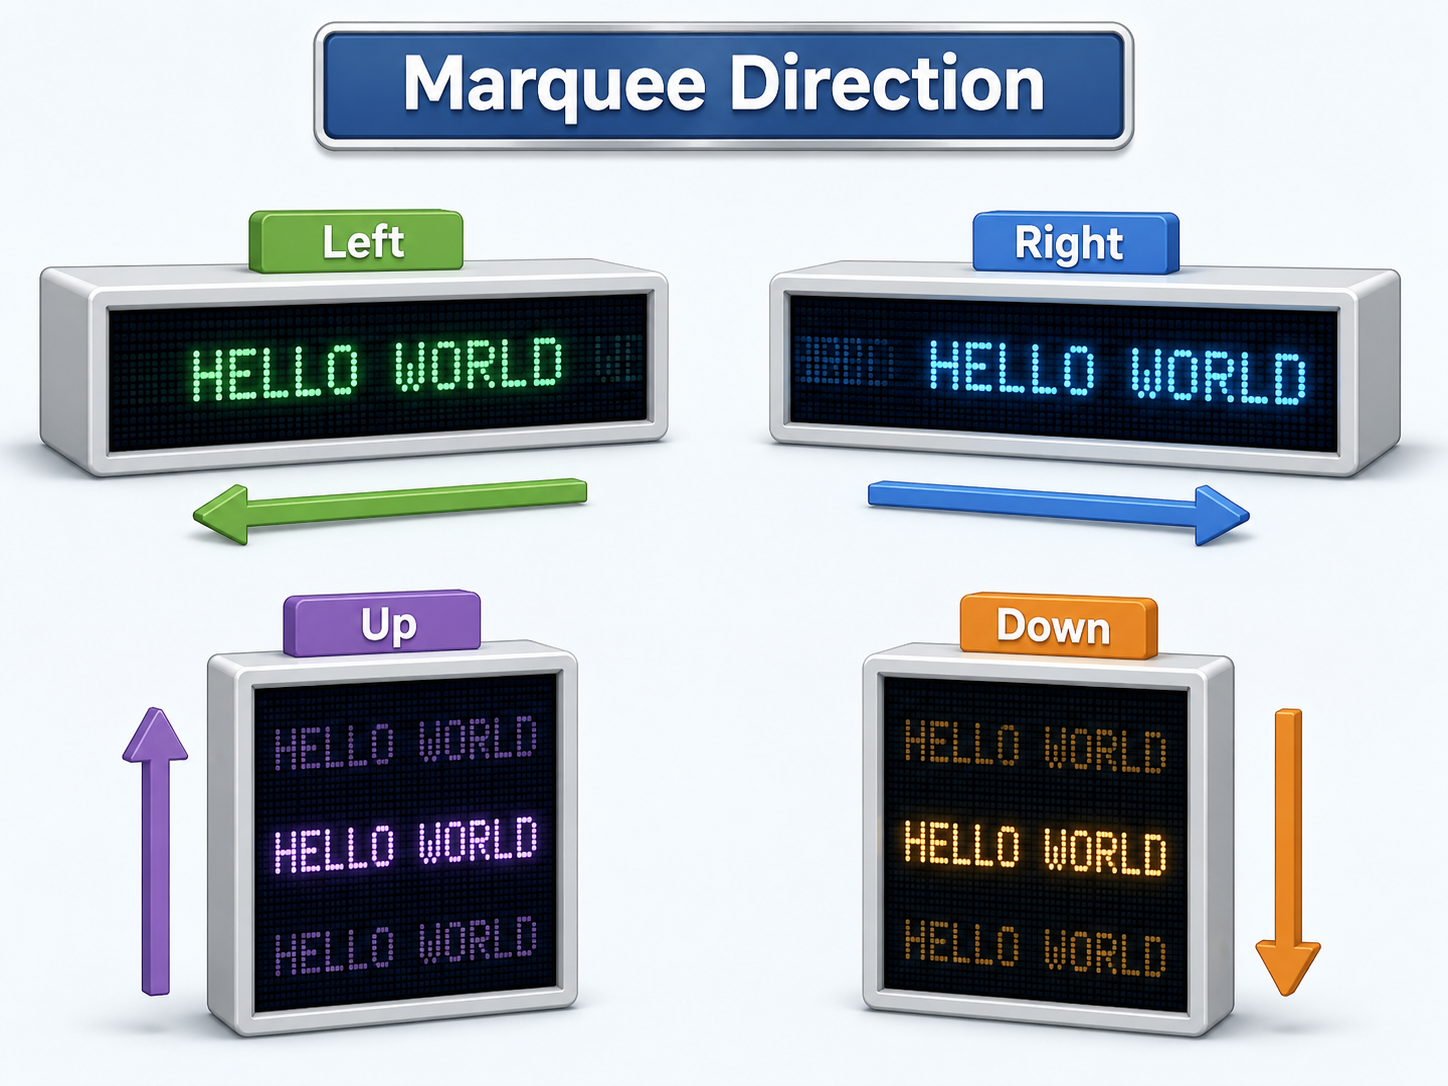
\includegraphics[width=\linewidth,height=.24\textheight,keepaspectratio]{chapters/Chapter04/topics/images/3d_marquee_direction.png}
}{
\fbox{\parbox{0.92\linewidth}{\centering\vspace{0.4cm}
\textbf{চিত্র}\\
ফাইল: \texttt{chapters/Chapter04/topics/images/3d\_marquee\_direction.png}
\vspace{0.4cm}}}
}
\captionof{figure}{চলমান লেখার ট্যাগের \texttt{direction} অ্যাট্রিবিউট}
\end{minipage}\hfill
\begin{minipage}[t]{.46\linewidth}\vspace{0pt}\small
\begin{keypointbox}{চিত্র ব্যাখ্যা}
চিত্রে লেখার চলার চারটি দিক দেখানো হয়েছে। \texttt{left} বামে, \texttt{right} ডানে, \texttt{up} উপরে এবং \texttt{down} নিচে চলার নির্দেশ দেয়।
\end{keypointbox}

\begin{keypointbox}{চিত্র দেখে কোড লেখার ধাপ}
\texttt{<marquee>}-এর ভেতরের লেখা বা ছবি চলমান থাকে। \texttt{direction} অ্যাট্রিবিউটের মান চলার দিক নির্ধারণ করে।
\end{keypointbox}
\end{minipage}\par


\begin{examplebox}{বিশেষভাবে দেখানো HTML কোড}
\par\noindent\begin{minipage}{\linewidth}
\begin{verbatim}
<marquee direction="left">Welcome to HSC ICT</marquee>
<marquee direction="right">HTML Marquee Example</marquee>
<marquee direction="up" height="80">Move Up</marquee>
<marquee direction="down" height="80">Move Down</marquee>
\end{verbatim}
\end{minipage}\par
\end{examplebox}

\begin{mistakebox}{আধুনিক সতর্কতা}
\texttt{<marquee>} বর্তমান HTML-এ পুরোনো ও নতুন কোডে ব্যবহারযোগ্য নয় এমন বৈশিষ্ট্য। পরীক্ষার উদাহরণ বোঝার জন্য এটি জানা দরকার। নতুন ওয়েবসাইটে চলমান দৃশ্যের জন্য CSS অ্যানিমেশন ব্যবহার করা হয়।
\end{mistakebox}

\subsection{লেখা বিন্যাসের ট্যাগ ও কাজ}

\begin{center}
\footnotesize
\begin{tabular}{|p{0.17\textwidth}|p{0.30\textwidth}|p{0.37\textwidth}|}
\hline
\textbf{ট্যাগ} & \textbf{কাজ} & \textbf{উদাহরণ} \\
\hline
\texttt{<h1>--<h6>} & শিরোনাম তৈরি করে & \texttt{<h1>Title</h1>} \\
\hline
\texttt{<p>} & অনুচ্ছেদ তৈরি করে & \texttt{<p>Text</p>} \\
\hline
\texttt{<br>} & নতুন লাইন তৈরি করে & \texttt{Line 1<br>Line 2} \\
\hline
\texttt{<hr>} & অনুভূমিক লাইন তৈরি করে & \texttt{<hr>} \\
\hline
\texttt{<b>} & মোটা অক্ষরের লেখা & \texttt{<b>Bold</b>} \\
\hline
\texttt{<strong>} & গুরুত্বপূর্ণ লেখা & \texttt{<strong>Important</strong>} \\
\hline
\texttt{<i>} & বাঁকা অক্ষরের লেখা & \texttt{<i>Italic</i>} \\
\hline
\texttt{<em>} & জোর দেওয়া লেখা & \texttt{<em>Emphasis</em>} \\
\hline
\texttt{<u>} & নিচে রেখাযুক্ত লেখা & \texttt{<u>Underline</u>} \\
\hline
\texttt{<ins>} & যোগ করা লেখা & \texttt{<ins>New</ins>} \\
\hline
\texttt{<del>} & বাদ দেওয়া লেখা & \texttt{<del>Old</del>} \\
\hline
\texttt{<s>} & মাঝে রেখাযুক্ত & \texttt{<s>Old</s>} \\
\hline
\texttt{<strike>} & মাঝে রেখাযুক্ত পুরোনো ট্যাগ & \texttt{<strike>Old</strike>} \\
\hline
\texttt{<small>} & ছোট লেখা & \texttt{<small>Small</small>} \\
\hline
\texttt{<big>} & বড় লেখা & \texttt{<big>Big</big>} \\
\hline
\texttt{<sub>} & নিচের সূচক & \texttt{H<sub>2</sub>O} \\
\hline
\texttt{<sup>} & উপরের সূচক & \texttt{a<sup>2</sup>} \\
\hline
\texttt{<pre>} & উৎসের বিন্যাস অক্ষুণ্ণ রাখা লেখা & \texttt{<pre>Text</pre>} \\
\hline
\texttt{<font>} & অক্ষরের আকার, রং ও ফন্টের ধরন & \texttt{<font color="red">Text</font>} \\
\hline
\end{tabular}
\normalsize
\end{center}

% Original applied explanation; see Chapter04/SOURCES.md.
\subsubsection{নোটিশের গুরুত্ব ও দেখতে মোটা লেখার পার্থক্য}
\begin{flushleft}\small
\begin{tabularx}{\linewidth}{|p{26mm}|X|X|}\hline
\textbf{বিবেচনা} & \textbf{\texttt{strong}} & \textbf{\texttt{b}}\\\hline
অর্থ & বিষয়বস্তুর বিশেষ গুরুত্ব গঠনে প্রকাশ করে & সাধারণভাবে দৃষ্টি আকর্ষণের অংশ চিহ্নিত করে\\\hline
দেখতে কেমন & মোটা দেখা যেতে পারে & প্রায় একইভাবে মোটা দেখা যেতে পারে; অর্থ এক নয়\\\hline
\end{tabularx}
\end{flushleft}
\textbf{উদাহরণ:} ভর্তি-নোটিশে \textbf{আবেদনের শেষ দিন} বিশেষ গুরুত্বপূর্ণ। \texttt{strong} দিয়ে সেই গুরুত্ব গঠনে প্রকাশ করা যায়।

নতুন বিষয় শুরু করতে শিরোনাম এবং বিস্তারিত লিখতে অনুচ্ছেদ ব্যবহার করবে। ফাঁকা জায়গা বানাতে বারবার \texttt{br} ব্যবহার করলে ছোট পর্দায় বিন্যাস অনিয়মিত হতে পারে। আলাদা অনুচ্ছেদে \texttt{p}, আর চিঠির ঠিকানার মতো একই অংশে প্রয়োজনীয় লাইনবিরতিতে \texttt{br} বেছে নেবে।


\subsection{পূর্ণাঙ্গ উদাহরণ}

\Needspace{6\baselineskip}
\par\noindent{\color{chFourTeal}\bfseries\small কোড: বাম কলাম শেষে ডান কলাম পড়বে}\par
\begin{multicols}{2}
\begin{verbatim}
<body bgcolor="#F5F5F5">

  <h1 align="center">HSC ICT Chapter 4</h1>
  <hr>

  <p>This is a normal paragraph.</p>
  <p><b>This is bold text.</b></p>
  <p><strong>This is important text.</strong></p>
  <p><i>This is italic text.</i></p>
  <p><em>This text is emphasized.</em></p>
  <p><u>This is underline text.</u></p>
  <p><small>This is small text.</small></p>
  <p><big>This is big text.</big></p>

  <p>Water formula: H<sub>2</sub>O</p>
  <p>Math formula: a<sup>2</sup> + b<sup>2</sup></p>

  <p><del>Old Notice</del> <ins>New Notice</ins></p>
  <p><s>Cancelled class</s></p>
  <p><strike>Old HTML tag</strike></p>

  <font size="5" color="blue" face="Arial">
    This text uses font tag.
  </font>

  <pre>
Name      Roll
Sakib     01
Asraful   02
  </pre>

</body>
\end{verbatim}
\end{multicols}


\begin{examplebox}{ফল কী হবে?}
ব্রাউজারে কেন্দ্রে সাজানো শিরোনাম, অনুভূমিক লাইন, মোটা অক্ষরের/বাঁকা অক্ষরের/নিচে রেখাযুক্ত লেখা, H\textsubscript{2}O নিচের সূচক, a\textsuperscript{2}+b\textsuperscript{2} উপরের সূচক, বাদ দেওয়া/যোগ করা লেখা, নীল Arial ফন্ট লেখা এবং আগের বিন্যাসে রাখা সারণির মতো লেখা দেখা যাবে।
\end{examplebox}

\begin{mistakebox}{সাধারণ ভুল}
\par\noindent
\begin{minipage}[t]{.48\linewidth}\vspace{0pt}
\begin{itemize}
\item \texttt{<br>} ট্যাগকে কন্টেইনার ট্যাগ মনে করা।
\item \texttt{<title>} আর \texttt{<h1>} একই মনে করা।
\item \texttt{<b>} ও \texttt{<strong>} ট্যাগের অর্থের পার্থক্য না বোঝা।
\item \texttt{<i>} ও \texttt{<em>} ট্যাগের অর্থগত পার্থক্য না বোঝা।
\end{itemize}
\end{minipage}\hfill
\begin{minipage}[t]{.48\linewidth}\vspace{0pt}
\begin{itemize}
\item \texttt{<sub>} আর \texttt{<sup>} উল্টো করে ফেলা।
\item \texttt{<font>} ট্যাগ আধুনিক HTML-এ বর্তমান মানে ব্যবহারযোগ্য নয় - এই বাড়তি তথ্য না দেওয়া।
\item বাংলা লেখা ঠিক দেখাতে \texttt{UTF-8} না দেওয়া।
\item ট্যাগ ঠিকভাবে বন্ধ না করা।
\end{itemize}
\end{minipage}\par

\end{mistakebox}


\begin{keypointbox}{শিরোনামের স্তর ঠিক রাখবে}
কলেজের পেজের মূল বিষয় \texttt{h1}, তার বিভাগ \texttt{h2} এবং সেই বিভাগের উপবিষয় \texttt{h3} হতে পারে। শুধু ছোট অক্ষর চাই বলে \texttt{h1} থেকে সরাসরি \texttt{h6}-এ যাওয়া ঠিক নয়। যৌক্তিক শিরোনাম স্ক্রিন রিডার ব্যবহারকারীকে পেজের অংশ বুঝতে সাহায্য করে; অক্ষরের দৃশ্যমান মাপ CSS-এ ঠিক করবে।
\end{keypointbox}


\subsection{সংক্ষিপ্ত অনুশীলন}

% Each question keeps its answer beneath it in the same column.
\begin{multicols}{2}
\noindent\begin{minipage}[t]{\linewidth}\vspace{0pt}
\chFourReviewQuestion{শিরোনাম ট্যাগ কয়টি?}
\end{minipage}\par\smallskip
\noindent\begin{minipage}[t]{\linewidth}\vspace{0pt}
\chFourReviewQuestion{অনুচ্ছেদ লেখার ট্যাগ কোনটি?}
\end{minipage}\par\smallskip
\noindent\begin{minipage}[t]{\linewidth}\vspace{0pt}
\chFourReviewQuestion{লাইন বিরতি করার ট্যাগ কোনটি?}
\end{minipage}\par\smallskip
\noindent\begin{minipage}[t]{\linewidth}\vspace{0pt}
\chFourReviewQuestion{অনুভূমিক লাইন তৈরির ট্যাগ কোনটি?}
\end{minipage}\par\smallskip
\noindent\begin{minipage}[t]{\linewidth}\vspace{0pt}
\chFourReviewQuestion{লেখা মোটা অক্ষরের করতে কোন ট্যাগ ব্যবহার হয়?}
\end{minipage}\par\smallskip
\noindent\begin{minipage}[t]{\linewidth}\vspace{0pt}
\chFourReviewQuestion{লেখা বাঁকা অক্ষরের করতে কোন ট্যাগ ব্যবহার হয়?}
\end{minipage}\par\smallskip
\noindent\begin{minipage}[t]{\linewidth}\vspace{0pt}
\chFourReviewQuestion{H\textsubscript{2}O লেখার জন্য কোন ট্যাগ ব্যবহার হবে?}
\end{minipage}\par\smallskip
\noindent\begin{minipage}[t]{\linewidth}\vspace{0pt}
\chFourReviewQuestion{a\textsuperscript{2} লেখার জন্য কোন ট্যাগ ব্যবহার হবে?}
\end{minipage}\par\smallskip
\noindent\begin{minipage}[t]{\linewidth}\vspace{0pt}
\chFourReviewQuestion{\texttt{<font>} ট্যাগের অ্যাট্রিবিউট কী কী?}
\end{minipage}\par\smallskip
\end{multicols}

\Needspace{10\baselineskip}
\subsection{পরীক্ষাভিত্তিক বহুনির্বাচনি প্রশ্ন}

\begin{multicols}{2}
\begin{enumerate}[leftmargin=*,itemsep=5pt]
\item \begin{minipage}[t]{\linewidth}\vspace{0pt}
ব্রাউজারের স্বাভাবিক রীতিতে সবচেয়ে বড় শিরোনাম কোনটি?
\par ক) \texttt{<h6>}
\par খ) \texttt{<h3>}
\par গ) \texttt{<h1>}
\par ঘ) \texttt{<head>}
\end{minipage}

\item \begin{minipage}[t]{\linewidth}\vspace{0pt}
অনুচ্ছেদ ট্যাগ কোনটি?
\par ক) \texttt{<para>}
\par খ) \texttt{<p>}
\par গ) \texttt{<br>}
\par ঘ) \texttt{<hr>}
\end{minipage}

\item \begin{minipage}[t]{\linewidth}\vspace{0pt}
নতুন লাইন তৈরি করতে কোন ট্যাগ ব্যবহৃত হয়?
\par ক) \texttt{<br>}
\par খ) \texttt{<b>}
\par গ) \texttt{<i>}
\par ঘ) \texttt{<u>}
\end{minipage}

\item \begin{minipage}[t]{\linewidth}\vspace{0pt}
H\textsubscript{2}O লেখার জন্য কোন ট্যাগ দরকার?
\par ক) \texttt{<sup>}
\par খ) \texttt{<sub>}
\par গ) \texttt{<small>}
\par ঘ) \texttt{<big>}
\end{minipage}

\item \begin{minipage}[t]{\linewidth}\vspace{0pt}
a\textsuperscript{2} লেখার জন্য কোন ট্যাগ দরকার?
\par ক) \texttt{<sub>}
\par খ) \texttt{<sup>}
\par গ) \texttt{<del>}
\par ঘ) \texttt{<ins>}
\end{minipage}

\item \begin{minipage}[t]{\linewidth}\vspace{0pt}
\texttt{<font>} ট্যাগের অ্যাট্রিবিউট কোনগুলো?
\par ক) \texttt{size}, \texttt{color}, \texttt{face}
\par খ) \texttt{src}, \texttt{alt}, \texttt{width}
\par গ) \texttt{href}, \texttt{target}, \texttt{title}
\par ঘ) \texttt{rowspan}, \texttt{colspan}, \texttt{border}
\end{minipage}
\end{enumerate}
\end{multicols}

\chFourMCQAnswer{১-গ, ২-খ, ৩-ক, ৪-খ, ৫-খ, ৬-ক}

% Density revision 2026-10-04: answers below questions; compact related content.
% ৪.x HTML তালিকা
\section{HTML-এ তালিকা (List)}

% Composition pass 2026-10-04
বইয়ের বিষয়গুলো একটানা অনুচ্ছেদে লিখলে আলাদা উপাদান ও তাদের ক্রম বোঝা কঠিন।

\chFourMotivation{তথ্যকে পৃথক উপাদানে সাজানো $\rightarrow$ তালিকা $\rightarrow$ ক্রম, বুলেট বা পরিভাষা–বর্ণনার জোড়া $\rightarrow$ লাইব্রেরির বিভাগ ও বইয়ের বিষয় দ্রুত পড়া যায়।}


\begin{learningbox}
এই অংশ শেষে শিক্ষার্থী পারবে:
\begin{itemize}
\item HTML তালিকা কী তা ব্যাখ্যা করতে।
\item ক্রমযুক্ত তালিকা, বুলেট তালিকা ও বর্ণনামূলক তালিকার পার্থক্য লিখতে।
\item \texttt{<ol>}, \texttt{<ul>}, \texttt{<li>}, \texttt{<dl>}, \texttt{<dt>} ও \texttt{<dd>} ট্যাগ ব্যবহার করতে।
\item \texttt{type} ও \texttt{start} অ্যাট্রিবিউটের কাজ বুঝতে।
\item নেস্টেড তালিকা তৈরি করতে।
\item HSC ব্যবহারিক অনুশীলন ও বোর্ড পরীক্ষার তালিকা-সম্পর্কিত প্রশ্নের উত্তর দিতে।
\end{itemize}
\end{learningbox}



\subsection{HTML তালিকা কী?}

\begin{definitionbox}{HTML তালিকা (List)}
ওয়েবপেজে একাধিক উপাদানকে ক্রম, বুলেট কিংবা পরিভাষা ও বর্ণনার জোড়ায় সাজানোর পদ্ধতিকে HTML তালিকা বলে।
\end{definitionbox}

পঠিত বিষয়, খাবারের মেনু, বই, রুটিন, পণ্যের বৈশিষ্ট্য, নির্দেশনার ধাপ ও ওয়েবসাইটের মেনু তালিকায় সাজানো যায়। পরিভাষা ও তার অর্থও তালিকায় দেখানো যায়। এতে প্রতিটি উপাদান আলাদা করে পড়া ও তুলনা করা সহজ হয়।




\subsection{HTML তালিকার প্রকারভেদ}

\begin{center}
\begin{tabular}{|p{0.25\textwidth}|p{0.18\textwidth}|p{0.43\textwidth}|}
\hline
\textbf{তালিকার ধরন} & \textbf{ট্যাগ} & \textbf{ব্যবহার} \\
\hline
ক্রমযুক্ত তালিকা & \texttt{<ol>} & সংখ্যা, অক্ষর বা রোমান সংখ্যা চিহ্নসহ ক্রমানুসার তালিকা \\
\hline
বুলেট তালিকা & \texttt{<ul>} & বুলেট/চিহ্নসহ তালিকা; উপাদানের ক্রম গুরুত্বপূর্ণ নয় \\
\hline
বর্ণনামূলক তালিকা & \texttt{<dl>} & পরিভাষা ও বর্ণনা আকারে তালিকা \\
\hline
\end{tabular}
\end{center}

\begin{keypointbox}{মনে রাখো}
\texttt{<ol>} ও \texttt{<ul>} তালিকার প্রতিটি উপাদান লেখার জন্য \texttt{<li>} ট্যাগ ব্যবহার করা হয়। কিন্তু \texttt{<dl>} তালিকায় \texttt{<li>} নয়; পরিভাষার জন্য \texttt{<dt>} এবং বর্ণনার জন্য \texttt{<dd>} ব্যবহার করা হয়।
\end{keypointbox}

\subsection{ক্রমযুক্ত তালিকা: \texttt{<ol>}}

\begin{definitionbox}{ক্রমযুক্ত তালিকা (Ordered List)}
যে তালিকায় উপাদানগুলো নির্দিষ্ট ক্রমে সংখ্যা, অক্ষর বা রোমান সংখ্যার চিহ্নসহ দেখানো হয়, তাকে ক্রমযুক্ত তালিকা বলে।
\end{definitionbox}

উপাদানের ক্রম গুরুত্বপূর্ণ হলে ক্রমযুক্ত তালিকা ব্যবহার করা হয়। নির্দেশনার ধাপ, পরীক্ষার রুটিন, স্থানক্রম, অধ্যায়ের তালিকা, ভর্তি প্রক্রিয়া ও অ্যালগরিদমের ধাপ এর উদাহরণ।

\subsubsection{সিনট্যাক্স}

\begin{examplebox}{কোড}
\par\noindent\begin{minipage}{\linewidth}
\begin{verbatim}
<ol>
  <li>First item</li>
  <li>Second item</li>
  <li>Third item</li>
</ol>
\end{verbatim}
\end{minipage}\par
\end{examplebox}

\subsubsection{উদাহরণ}

% Split revision: code and its explanation share one row.
\par\noindent
\begin{minipage}[t]{.54\linewidth}\vspace{0pt}\small
\textbf{\color{chFourTeal}কোড}\par
\begin{verbatim}
<!DOCTYPE html>
<html>
<body>
  <h2>HSC ICT Chapter List</h2>

  <ol>
    <li>ICT: World and Bangladesh Perspective</li>
    <li>Communication System and Networking</li>
    <li>Number System and Digital Device</li>
    <li>Web Design Introduction and HTML</li>
  </ol>
</body>
</html>
\end{verbatim}

\par\smallskip
\end{minipage}\hfill
\begin{minipage}[t]{.42\linewidth}\vspace{0pt}\small
\textbf{\color{chFourTeal}ফল ও ব্যাখ্যা}\par
\textbf{ফল:}
\begin{enumerate}
\item ICT: World and Bangladesh Perspective
\item Communication System and Networking
\item Number System and Digital Device
\item Web Design Introduction and HTML
\end{enumerate}
\textbf{ব্যাখ্যা:} \texttt{<ol>} ক্রমযুক্ত তালিকা শুরু করে এবং প্রতিটি \texttt{<li>} একটি করে তালিকার উপাদান তৈরি করে। ব্রাউজার স্বাভাবিক অবস্থায় চিহ্ন হিসেবে 1, 2, 3 ব্যবহার করে।
\par\smallskip
\end{minipage}\par


\subsection{ক্রমযুক্ত তালিকার অ্যাট্রিবিউট}

\subsubsection{\texttt{type} অ্যাট্রিবিউট}

\texttt{type} অ্যাট্রিবিউট দিয়ে ক্রমযুক্ত তালিকার চিহ্ন কীভাবে দেখাবে তা নির্ধারণ করা যায়।

\begin{center}
\begin{tabular}{|p{0.25\textwidth}|p{0.35\textwidth}|}
\hline
\textbf{ধরন} & \textbf{ফলের চিহ্ন} \\
\hline
\texttt{type="1"} & 1, 2, 3 \\
\hline
\texttt{type="A"} & A, B, C \\
\hline
\texttt{type="a"} & a, b, c \\
\hline
\texttt{type="I"} & I, II, III \\
\hline
\texttt{type="i"} & i, ii, iii \\
\hline
\end{tabular}
\end{center}

\begin{chFourWholeExample}{কোড ও ব্রাউজারে ফল}
\noindent
\begin{minipage}[t]{.50\linewidth}\vspace{0pt}

\begin{verbatim}
<ol type="A">
  <li>HTML</li>
  <li>CSS</li>
  <li>JavaScript</li>
</ol>
\end{verbatim}

\end{minipage}\hfill
\begin{minipage}[t]{.46\linewidth}\vspace{0pt}
\textbf{ফল:}\\
A. HTML\\
B. CSS\\
C. JavaScript\\
\end{minipage}
\chFourWhy{\texttt{type="A"} দেওয়ায় চিহ্ন সংখ্যা না হয়ে বড় হাতের অক্ষর হিসেবে দেখায়।}
\end{chFourWholeExample}

\subsubsection{\texttt{start} অ্যাট্রিবিউট}

\texttt{start} অ্যাট্রিবিউট দিয়ে ক্রমযুক্ত তালিকা কোন সংখ্যা থেকে শুরু হবে তা নির্ধারণ করা যায়।

\begin{chFourWholeExample}{কোড ও ব্রাউজারে ফল}
\noindent
\begin{minipage}[t]{.50\linewidth}\vspace{0pt}

\begin{verbatim}
<ol start="5">
  <li>HTML</li>
  <li>CSS</li>
  <li>JavaScript</li>
</ol>
\end{verbatim}

\end{minipage}\hfill
\begin{minipage}[t]{.46\linewidth}\vspace{0pt}
\textbf{ফল:}
\begin{enumerate}[start=5]
\item HTML
\item CSS
\item JavaScript
\end{enumerate}
\end{minipage}
\chFourWhy{\texttt{start="5"} দেওয়ায় তালিকার চিহ্ন ১ থেকে না শুরু হয়ে ৫ থেকে শুরু হয়েছে।}
\end{chFourWholeExample}

\begin{keypointbox}{মান অনুযায়ী বাড়তি তথ্য}
\texttt{reversed} অ্যাট্রিবিউট দিলে ক্রমযুক্ত তালিকা উল্টো ক্রমে গণনা হয়।
নির্দিষ্ট উপাদান থেকে গণনার মান বদলাতে সেই \texttt{<li>} এলিমেন্টে \texttt{value} অ্যাট্রিবিউট ব্যবহার করা যায়।
\end{keypointbox}



\subsection{বুলেট তালিকা: \texttt{<ul>}}

\begin{definitionbox}{বুলেট তালিকা (Unordered List)}
যে তালিকায় উপাদানের নির্দিষ্ট ক্রম গুরুত্বপূর্ণ নয় এবং প্রতিটি উপাদান বুলেট বা চিহ্নসহ দেখানো হয়, তাকে বুলেট তালিকা বলে।
\end{definitionbox}

যখন উপাদানের ক্রম গুরুত্বপূর্ণ নয়, তখন বুলেট তালিকা ব্যবহার করা হয়। যেমন: মেনু, বৈশিষ্ট্য, পঠিত বিষয়, কেনাকাটা, বিজ্ঞপ্তি, গুরুত্বপূর্ণ পাঠ বা ওয়েবসাইটে চলাচলের তালিকা।

\subsubsection{সিনট্যাক্স}

\begin{examplebox}{কোড}
\par\noindent\begin{minipage}{\linewidth}
\begin{verbatim}
<ul>
  <li>Item one</li>
  <li>Item two</li>
  <li>Item three</li>
</ul>
\end{verbatim}
\end{minipage}\par
\end{examplebox}

\subsubsection{উদাহরণ}

\begin{chFourWholeExample}{কোড ও ব্রাউজারে ফল}
\noindent
\begin{minipage}[t]{.50\linewidth}\vspace{0pt}

\begin{verbatim}
<h2>Web Design Tools</h2>

<ul>
  <li>HTML</li>
  <li>CSS</li>
  <li>JavaScript</li>
  <li>Browser</li>
</ul>
\end{verbatim}

\end{minipage}\hfill
\begin{minipage}[t]{.46\linewidth}\vspace{0pt}
\textbf{ফল:}
\begin{itemize}
\item HTML
\item CSS
\item JavaScript
\item Browser
\end{itemize}
\end{minipage}
\chFourWhy{\texttt{<ul>} বুলেট তালিকা তৈরি করে। ব্রাউজার স্বাভাবিক অবস্থায় বুলেট চিহ্ন দেখায়।}
\end{chFourWholeExample}

\subsection{বুলেট তালিকার \texttt{type} অ্যাট্রিবিউট}

পরীক্ষায় পরিচিত পুরোনো HTML কোডে বুলেট তালিকার চিহ্ন পরিবর্তনের জন্য \texttt{type} অ্যাট্রিবিউট দেখা যায়।

\begin{center}
\begin{tabular}{|p{0.30\textwidth}|p{0.34\textwidth}|}
\hline
\textbf{ধরন} & \textbf{ফল কী হবে?} \\
\hline
\texttt{type="disc"} & ভরাট বুলেট \\
\hline
\texttt{type="circle"} & ফাঁপা গোলাকার বুলেট \\
\hline
\texttt{type="square"} & বর্গাকার বুলেট \\
\hline
\end{tabular}
\end{center}

\begin{chFourWholeExample}{কোড ও ব্রাউজারে ফল}
\noindent
\begin{minipage}[t]{.50\linewidth}\vspace{0pt}

\begin{verbatim}
<ul type="square">
  <li>Monitor</li>
  <li>Keyboard</li>
  <li>Mouse</li>
</ul>
\end{verbatim}

\end{minipage}\hfill
\begin{minipage}[t]{.46\linewidth}\vspace{0pt}
\textbf{ফল:}\\
\(\blacksquare\) Monitor\\
\(\blacksquare\) Keyboard\\
\(\blacksquare\) Mouse\\
\end{minipage}
\chFourWhy{\texttt{type="square"} দেওয়ায় তালিকার চিহ্ন বর্গাকার বুলেট আকারে দেখা যাবে।}
\end{chFourWholeExample}

\begin{mistakebox}{আধুনিক HTML-এর নিয়ম}
বর্তমান HTML-এ \texttt{<ul>}-এর \texttt{type} পুরোনো অ্যাট্রিবিউট; বুলেটের ধরন বদলাতে CSS-এর \texttt{list-style-type} ব্যবহার করা হয়। \texttt{<ol>}-এর \texttt{type} কিন্তু বর্তমান মানে বৈধ। পরীক্ষার পুরোনো উদাহরণ বোঝার জন্য \texttt{type="disc"}, \texttt{type="circle"} ও \texttt{type="square"} জানা দরকার।
\end{mistakebox}



\subsection{তালিকার উপাদান: \texttt{<li>}}

\begin{definitionbox}{তালিকার উপাদান (List Item)}
\texttt{<li>} ট্যাগ তালিকার প্রতিটি উপাদান লিখতে ব্যবহৃত হয়।
\end{definitionbox}

\texttt{<ol>} এবং \texttt{<ul>} - দুই ধরনের তালিকার উপাদান লিখতেই \texttt{<li>} ট্যাগ ব্যবহার করা হয়।

\begin{chFourWholeExample}{কোড ও ব্রাউজারে ফল}
\noindent
\begin{minipage}[t]{.50\linewidth}\vspace{0pt}

\begin{verbatim}
<ul>
  <li>Bangla</li>
  <li>English</li>
  <li>ICT</li>
</ul>
\end{verbatim}

\end{minipage}\hfill
\begin{minipage}[t]{.46\linewidth}\vspace{0pt}
\textbf{ফল:}
\begin{itemize}
\item Bangla
\item English
\item ICT
\end{itemize}
\end{minipage}
\chFourWhy{প্রতিটি \texttt{<li>} ট্যাগ একটি আলাদা তালিকার উপাদান তৈরি করেছে।}
\end{chFourWholeExample}

\begin{keypointbox}{পরীক্ষায় মনে রাখবে}
HTML-এর নির্দিষ্ট নিয়মে \texttt{</li>} বাদ দেওয়া যায়; যেমন পরেই আরেকটি \texttt{<li>} শুরু হলে। এটি শুধু পুরোনো HTML-এর নিয়ম নয়। শেখার সময় \texttt{<li>Item</li>} আকারে শেষের ট্যাগ লিখলে তালিকার গঠন সহজে বোঝা যায়।
\end{keypointbox}

\subsection{বর্ণনামূলক তালিকা: \texttt{<dl>}, \texttt{<dt>}, \texttt{<dd>}}

\begin{definitionbox}{বর্ণনামূলক তালিকা (Description List)}
পরিভাষা বা বিষয়ের নামের সঙ্গে তার বর্ণনা সাজিয়ে দেখানোর তালিকাকে বর্ণনামূলক তালিকা বলে।
\end{definitionbox}

পরিভাষা, সংজ্ঞা, বহুল জিজ্ঞাসিত প্রশ্ন (Frequently Asked Questions বা FAQ), পণ্যের বৈশিষ্ট্য, যোগাযোগের বিস্তারিত তথ্য বা শব্দের অর্থ দেখাতে বর্ণনামূলক তালিকা ব্যবহার করা যায়।

\subsubsection{সিনট্যাক্স}

% Split revision: code and its explanation share one row.
\par\noindent
\begin{minipage}[t]{.50\linewidth}\vspace{0pt}\small
\textbf{\color{chFourTeal}কোড}\par
\begin{verbatim}
<dl>
  <dt>Term</dt>
  <dd>Description of the term</dd>
</dl>
\end{verbatim}

\par\smallskip
\end{minipage}\hfill
\begin{minipage}[t]{.46\linewidth}\vspace{0pt}\small
\begin{tabular}{|p{0.25\linewidth}|p{0.64\linewidth}|}
\hline
\textbf{ট্যাগ} & \textbf{কাজ} \\
\hline
\texttt{<dl>} & বর্ণনামূলক তালিকা শুরু ও শেষ করে \\
\hline
\texttt{<dt>} & পরিভাষা বা নাম নির্দেশ করে \\
\hline
\texttt{<dd>} & পরিভাষার বর্ণনা নির্দেশ করে \\
\hline
\end{tabular}
\end{minipage}\par


% Split revision: code and its explanation share one row.
\par\noindent
\begin{minipage}[t]{.54\linewidth}\vspace{0pt}\small
\subsubsection{উদাহরণ: কোড}
\begin{verbatim}
<h2>Web Terms</h2><dl>
  <dt>HTML</dt>
  <dd>HTML is used to create the structure of a web page.</dd>
  <dt>CSS</dt>
  <dd>CSS is used to design and style a web page.</dd>
  <dt>JavaScript</dt>
  <dd>JavaScript is used to add interactivity to a web page.</dd></dl>
\end{verbatim}

\par\smallskip
\end{minipage}\hfill
\begin{minipage}[t]{.42\linewidth}\vspace{0pt}\small
\textbf{\color{chFourTeal}ফল ও ব্যাখ্যা}\par
\textbf{HTML}\\
\hspace*{.5em}HTML is used to create the structure of a web page.\\
\textbf{CSS}\\
\hspace*{.5em}CSS is used to design and style a web page.\\
\textbf{JavaScript}\\
\hspace*{.5em}JavaScript is used to add interactivity to a web page.\\
\textbf{ব্যাখ্যা:} \texttt{<dt>} ট্যাগ পরিভাষা দেখায় এবং \texttt{<dd>} ট্যাগ সেই পরিভাষার বর্ণনা দেখায়।
\par\smallskip
\end{minipage}\par




\begin{keypointbox}{মান অনুযায়ী বাড়তি তথ্য}
একটি \texttt{dl} এলিমেন্টে একই দলভুক্ত একাধিক নাম বা পরিভাষার জন্য একাধিক \texttt{dt} এবং সংশ্লিষ্ট বিকল্প বর্ণনার জন্য একাধিক \texttt{dd} দেওয়া যায়। একই বর্ণনার একাধিক অনুচ্ছেদ হলে সেগুলো একই \texttt{dd}-এর মধ্যে থাকে। প্রয়োজন হলে প্রতিটি নাম-বর্ণনার দলকে \texttt{div} দিয়ে ঘিরে রীতি বা মেটাডেটা দেওয়া যায়।
\end{keypointbox}

% Original applied explanation; see Chapter04/SOURCES.md.
\subsubsection{তালিকার ধরন বাছাইয়ে একটি সহজ পরীক্ষা}
ভর্তি-আবেদনের ধাপ উল্টে দিলে কাজ বদলে যায়; সেখানে \texttt{ol} উপযোগী। প্রয়োজনীয় কাগজপত্রের তালিকায় ক্রম সাধারণত জরুরি নয়; সেখানে \texttt{ul} উপযোগী। পরিভাষা ও তার ব্যাখ্যা জোড়া আকারে রাখতে \texttt{dl}, \texttt{dt} ও \texttt{dd} লাগে।

বিভাগের তালিকার ভেতরে বিষয়ের উপতালিকা বসালে উপতালিকাটি সংশ্লিষ্ট \texttt{li}-এর ভেতরে রাখবে। এতে কোন বিষয় কোন বিভাগের অধীন, তা গঠনে প্রকাশ পায়। শুধু স্পেস দিয়ে লেখা সরিয়ে একই সম্পর্ক নির্ভরযোগ্যভাবে প্রকাশ করা যায় না।


\subsection{নেস্টেড তালিকা}

\begin{definitionbox}{নেস্টেড তালিকা (Nested List)}
একটি তালিকার উপাদানের ভিতরে আরেকটি তালিকা ব্যবহার করলে তাকে নেস্টেড তালিকা বলা যায়।
\end{definitionbox}

% Split revision: code and its explanation share one row.
\par\noindent
\begin{minipage}[t]{.50\linewidth}\vspace{0pt}\small
\textbf{\color{chFourTeal}কোড}\par
\par\noindent
\begin{verbatim}
<ul>
  <li>Science
    <ol>
      <li>Physics</li>
      <li>Chemistry</li>
      <li>Biology</li>
    </ol>
  </li>

  <li>Business Studies
    <ol>
      <li>Accounting</li>
      <li>Finance</li>
      <li>Management</li>
    </ol>
  </li>
</ul>
\end{verbatim}
\par
\par\smallskip
\end{minipage}\hfill
\begin{minipage}[t]{.46\linewidth}\vspace{0pt}\small
\textbf{\color{chFourTeal}ফল ও ব্যাখ্যা}\par
\textbf{ফল:}
\begin{itemize}
\item Science
  \begin{enumerate}
  \item Physics
  \item Chemistry
  \item Biology
  \end{enumerate}
\item Business Studies
  \begin{enumerate}
  \item Accounting
  \item Finance
  \item Management
  \end{enumerate}
\end{itemize}
\textbf{ব্যাখ্যা:} বাইরের তালিকাটি \texttt{<ul>} এবং প্রতিটি দলের ভিতরে \texttt{<ol>} তালিকা আছে। এইভাবে শ্রেণি ও উপশ্রেণি দেখানো যায়।
\par\smallskip
\end{minipage}\par


\begin{keypointbox}{নেস্টেড তালিকা কোথায় ব্যবহার হয়}
পঠিত বিষয়ের দল, ওয়েবসাইটের মেনু, অধ্যায় ও উপপাঠ, শ্রেণি ও উপশ্রেণি, কোর্সের অংশ বা পণ্যের বৈশিষ্ট্যের দল দেখাতে নেস্টেড তালিকা ব্যবহার করা যায়।
\end{keypointbox}

\subsection{ক্রমযুক্ত, বুলেট ও বর্ণনামূলক তালিকার পার্থক্য}

\begin{center}
\small
\begin{tabular}{|p{0.18\textwidth}|p{0.22\textwidth}|p{0.22\textwidth}|p{0.22\textwidth}|}
\hline
\textbf{বিষয়} & \textbf{ক্রমযুক্ত তালিকা} & \textbf{বুলেট তালিকা} & \textbf{বর্ণনামূলক তালিকা} \\
\hline
ট্যাগ & \texttt{<ol>} & \texttt{<ul>} & \texttt{<dl>} \\
\hline
উপাদান ট্যাগ & \texttt{<li>} & \texttt{<li>} & \texttt{<dt>}, \texttt{<dd>} \\
\hline
চিহ্ন & সংখ্যা/অক্ষর/রোমান সংখ্যা & বুলেট/চিহ্ন & পরিভাষা-বর্ণনা \\
\hline
ক্রম গুরুত্বপূর্ণ? & হ্যাঁ & না & পরিভাষা অনুযায়ী \\
\hline
ব্যবহার & ধাপ, স্থানক্রম, রুটিন & পাঠ, বৈশিষ্ট্য, মেনু & সংজ্ঞা, পরিভাষার তালিকা \\
\hline
উদাহরণ & 1, 2, 3 & বুলেট & HTML - মার্কআপ ভাষা \\
\hline
\end{tabular}
\normalsize
\end{center}

\subsection{পূর্ণাঙ্গ উদাহরণ}

\Needspace{6\baselineskip}
\par\noindent{\color{chFourTeal}\bfseries\small কোড: বাম কলাম শেষে ডান কলাম পড়বে}\par
\begin{multicols}{2}
\begin{verbatim}
<h1>HTML List Example</h1>

<h2>Ordered List</h2>
<ol type="1">
  <li>Open Notepad</li>
  <li>Write HTML code</li>
  <li>Save as index.html</li>
  <li>Open with browser</li>
</ol>

<h2>Unordered List</h2>
<ul type="square">
  <li>HTML</li>
  <li>CSS</li>
  <li>JavaScript</li>
</ul>

<h2>Description List</h2>
<dl>
  <dt>HTML</dt>
  <dd>HTML creates the structure of a web page.</dd>

  <dt>CSS</dt>
  <dd>CSS designs the appearance of a web page.</dd>
</dl>
\end{verbatim}
\end{multicols}


\begin{examplebox}{ফল কী হবে?}
ব্রাউজারে প্রথমে ক্রমযুক্ত তালিকা 1, 2, 3, 4 আকারে দেখা যাবে। এরপর বুলেট তালিকা বর্গাকার বুলেট আকারে দেখা যাবে। শেষে বর্ণনামূলক তালিকা পরিভাষা ও বর্ণনা আকারে দেখা যাবে।
\end{examplebox}


\begin{mistakebox}{সাধারণ ভুল}
\par\noindent
\begin{minipage}[t]{.48\linewidth}\vspace{0pt}
\begin{itemize}
\item \texttt{<ol>} ও \texttt{<ul>} গুলিয়ে ফেলা।
\item \texttt{<li>} ট্যাগ না দেওয়া।
\item \texttt{<dl>} ট্যাগের ভিতরে \texttt{<li>} ব্যবহার করা।
\item \texttt{<dt>} ও \texttt{<dd>} ভুলভাবে ব্যবহার করা।
\end{itemize}
\end{minipage}\hfill
\begin{minipage}[t]{.48\linewidth}\vspace{0pt}
\begin{itemize}
\item ক্রমযুক্ত তালিকায় \texttt{type} মান ভুল লেখা।
\item \texttt{<ul>} ট্যাগে সংখ্যা চিহ্ন আশা করা।
\item তালিকার শেষের ট্যাগ না দেওয়া।
\item নেস্টেড তালিকা ভুলভাবে বন্ধ করা।
\end{itemize}
\end{minipage}\par

\end{mistakebox}

\begin{boardbox}{নেস্টেড তালিকার সঠিক গঠন}
\begin{examplebox}{কোড}
\par\noindent\begin{minipage}{\linewidth}
\begin{verbatim}
<ul>
  <li>ICT
    <ol>
      <li>HTML</li>
      <li>Networking</li>
    </ol>
  </li>
</ul>
\end{verbatim}
\end{minipage}\par
\end{examplebox}
\end{boardbox}

% Technical basis: MDN ol. Inspired question skills, original data and wording.
\subsubsection{type ও start একসঙ্গে: ফল গণনা করার নিয়ম}
\texttt{type} চিহ্নের ধরন বেছে নেয়; \texttt{start} বলে কত নম্বর অবস্থান থেকে গণনা শুরু হবে। \texttt{start}-এর মান পূর্ণসংখ্যা, চিহ্নের অক্ষর নয়। যেমন \texttt{type="A" start="3"} দিলে প্রথম চিহ্ন C, পরেরটি D; \texttt{type="i" start="4"} দিলে iv, v। অক্ষর e থেকে শুরু করতে \texttt{type="a" start="5"} লিখবে, \texttt{start="e"} নয়।

\par\noindent{\color{chFourTeal}\bfseries\small কোড: বাম কলাম শেষে ডান কলাম পড়বে}\par
\begin{multicols}{2}
\begin{verbatim}
<ol type="a" start="4">
  <li>Books</li>
  <li>Courses
    <ol type="i" start="2">
      <li>HTML</li>
      <li>CSS</li>
    </ol>
  </li>
  <li>Clubs
    <ul style="list-style-type:circle">
      <li>Science</li>
      <li>Debate</li>
    </ul>
  </li>
</ol>
\end{verbatim}
\end{multicols}
\par\noindent\begin{minipage}[t]{.36\linewidth}\vspace{0pt}
\textbf{\color{chFourTeal}দৃশ্যমান ফল}\par
\begin{enumerate}[label=\alph*.,start=4,leftmargin=*]
\item Books
\item Courses
\begin{enumerate}[label=\roman*.,start=2,leftmargin=*]
\item HTML
\item CSS
\end{enumerate}
\item Clubs
\begin{itemize}[label=$\circ$,leftmargin=*]
\item Science
\item Debate
\end{itemize}
\end{enumerate}

\end{minipage}\hfill
\begin{minipage}[t]{.60\linewidth}\vspace{0pt}
বাইরের তালিকা d, e, f পর্যন্ত চলে। ভেতরের রোমান তালিকা নিজস্ব \texttt{start="2"} অনুযায়ী ii থেকে চলে; বাইরের e থেকে গণনা করে না। বুলেট তালিকা সংখ্যার গণনায় অংশ নেয় না। প্রতিটি ভেতরের তালিকা তার সংশ্লিষ্ট বাইরের \texttt{<li>}-এর মধ্যেই শেষ হয়েছে।
\end{minipage}\par

নেস্টেড তালিকার প্রতিটি স্তরে আলাদা \texttt{<ol>} বা \texttt{<ul>} থাকে। চিহ্নের ধরন ও শুরু নম্বর ওই স্তরেই নির্ধারিত হয়। ফলে বাইরের বড় হাতের অক্ষরের তালিকার ভেতরে সংখ্যা এবং অন্য শাখায় বুলেট রাখা যায়। স্তরের প্রথম দুটি চিহ্ন মিলিয়ে গণনা যাচাই করা যায়।



\subsection{সংক্ষিপ্ত অনুশীলন}

% Each question keeps its answer beneath it in the same column.
\begin{multicols}{2}
\noindent\begin{minipage}[t]{\linewidth}\vspace{0pt}
\chFourReviewQuestion{HTML তালিকা কী?}
\end{minipage}\par\smallskip
\noindent\begin{minipage}[t]{\linewidth}\vspace{0pt}
\chFourReviewQuestion{HTML-এ তালিকা কয় প্রকার?}
\end{minipage}\par\smallskip
\noindent\begin{minipage}[t]{\linewidth}\vspace{0pt}
\chFourReviewQuestion{ক্রমযুক্ত তালিকা তৈরির ট্যাগ কোনটি?}
\end{minipage}\par\smallskip
\noindent\begin{minipage}[t]{\linewidth}\vspace{0pt}
\chFourReviewQuestion{বুলেট তালিকা তৈরির ট্যাগ কোনটি?}
\end{minipage}\par\smallskip
\noindent\begin{minipage}[t]{\linewidth}\vspace{0pt}
\chFourReviewQuestion{তালিকার উপাদান লেখার ট্যাগ কোনটি?}
\end{minipage}\par\smallskip
\noindent\begin{minipage}[t]{\linewidth}\vspace{0pt}
\chFourReviewQuestion{বর্ণনামূলক তালিকা তৈরির ট্যাগ কোনটি?}
\end{minipage}\par\smallskip
\noindent\begin{minipage}[t]{\linewidth}\vspace{0pt}
\chFourReviewQuestion{বর্ণনামূলক তালিকায় পরিভাষা লেখার ট্যাগ কোনটি?}
\end{minipage}\par\smallskip
\noindent\begin{minipage}[t]{\linewidth}\vspace{0pt}
\chFourReviewQuestion{বর্ণনামূলক তালিকায় বর্ণনা লেখার ট্যাগ কোনটি?}
\end{minipage}\par\smallskip
\noindent\begin{minipage}[t]{\linewidth}\vspace{0pt}
\chFourReviewQuestion{\texttt{<ol type="A">} দিলে ফল কেমন হবে?}
\end{minipage}\par\smallskip
\noindent\begin{minipage}[t]{\linewidth}\vspace{0pt}
\chFourReviewQuestion{\texttt{<ul type="square">} দিলে ফল কেমন হবে?}
\end{minipage}\par\smallskip
\end{multicols}

\Needspace{10\baselineskip}
\subsection{পরীক্ষাভিত্তিক বহুনির্বাচনি প্রশ্ন}

\begin{multicols}{2}
\begin{enumerate}[leftmargin=*,itemsep=5pt]
\item \begin{minipage}[t]{\linewidth}\vspace{0pt}
HTML-এ তালিকা সাধারণত কয় প্রকার?
\par ক) ২
\par খ) ৩
\par গ) ৪
\par ঘ) ৫
\end{minipage}

\item \begin{minipage}[t]{\linewidth}\vspace{0pt}
ক্রমযুক্ত তালিকা তৈরির ট্যাগ কোনটি?
\par ক) \texttt{<ul>}
\par খ) \texttt{<ol>}
\par গ) \texttt{<li>}
\par ঘ) \texttt{<dl>}
\end{minipage}

\item \begin{minipage}[t]{\linewidth}\vspace{0pt}
বুলেট তালিকা তৈরির ট্যাগ কোনটি?
\par ক) \texttt{<ul>}
\par খ) \texttt{<ol>}
\par গ) \texttt{<dt>}
\par ঘ) \texttt{<dd>}
\end{minipage}

\item \begin{minipage}[t]{\linewidth}\vspace{0pt}
তালিকার উপাদান যুক্ত করার ট্যাগ কোনটি?
\par ক) \texttt{<ol>}
\par খ) \texttt{<li>}
\par গ) \texttt{<ul>}
\par ঘ) \texttt{<dl>}
\end{minipage}

\item \begin{minipage}[t]{\linewidth}\vspace{0pt}
বর্ণনামূলক তালিকায় পরিভাষা লেখার ট্যাগ কোনটি?
\par ক) \texttt{<dd>}
\par খ) \texttt{<dt>}
\par গ) \texttt{<li>}
\par ঘ) \texttt{<ul>}
\end{minipage}

\item \begin{minipage}[t]{\linewidth}\vspace{0pt}
\texttt{<ol type="i">} দিলে তালিকার চিহ্ন কেমন হবে?
\par ক) A, B, C
\par খ) a, b, c
\par গ) I, II, III
\par ঘ) i, ii, iii
\end{minipage}

\item \begin{minipage}[t]{\linewidth}\vspace{0pt}
বুলেট তালিকার চিহ্ন বর্গাকার করতে কোনটি ব্যবহার করা যায়?
\par ক) \texttt{<ul type="square">}
\par খ) \texttt{<ol type="square">}
\par গ) \texttt{<li type="A">}
\par ঘ) \texttt{<dl type="square">}
\end{minipage}
\end{enumerate}
\end{multicols}

\chFourMCQAnswer{১-খ, ২-খ, ৩-ক, ৪-খ, ৫-খ, ৬-ঘ, ৭-ক}

% Density revision 2026-10-04: answers below questions; compact related content.
% 4.x হাইপারলিংক in HTML
\section{HTML-এ হাইপারলিংক (Hyperlink)}

% Composition pass 2026-10-04
Home, Notice ও Result পেজ তৈরি আছে, কিন্তু এক পেজ থেকে অন্যটিতে যাওয়ার পথ দরকার।

\chFourMotivation{পেজে চলাচল $\rightarrow$ হাইপারলিংক $\rightarrow$ href-এ গন্তব্য ও ক্লিকযোগ্য লেখা/ছবি $\rightarrow$ কলেজের মেনু থেকে প্রয়োজনীয় পেজ খোলা।}


\begin{learningbox}
এই অংশ শেষে শিক্ষার্থী পারবে:
\begin{itemize}
\item হাইপারলিংক কী এবং ওয়েবপেজ চলাচলে এর প্রয়োজনীয়তা ব্যাখ্যা করতে।
\item \texttt{<a>} ট্যাগ ও \texttt{href} অ্যাট্রিবিউটের কাজ লিখতে।
\item অভ্যন্তরীণ, বাহ্যিক, বুকমার্ক, ইমেইল, ছবি, ফাইল ও নতুন ট্যাবের লিংক তৈরি করতে।
\item লিংকের লেখা, URL, \texttt{mailto:}, \texttt{target} ও \texttt{download} অ্যাট্রিবিউট ব্যবহার করতে।
\item পূর্ণ URL, আপেক্ষিক URL এবং নতুন ট্যাবে লিংক খোলার নিয়ম ব্যাখ্যা করতে।
\item HSC ব্যবহারিক অনুশীলন ও বোর্ড পরীক্ষার হাইপারলিংক-সম্পর্কিত প্রশ্নের উত্তর দিতে।
\end{itemize}
\end{learningbox}



HTML তালিকা শেখার পর হাইপারলিংক শেখা গুরুত্বপূর্ণ, কারণ একটি ওয়েবপেজের লেখা, তালিকা, ছবি বা বোতামের মাধ্যমে অন্য পেজ, ওয়েবসাইট, ফাইল বা একই পেজের নির্দিষ্ট অংশে যাওয়ার ব্যবস্থা হাইপারলিংক দিয়ে করা হয়। ওয়েবসাইটের চলাচল মেনু, ``Read more'', ``Download'', ``Contact us'', ছবি বোতাম - এসব হাইপারলিংকের বাস্তব উদাহরণ।

\subsection{হাইপারলিংক কী?}

\begin{definitionbox}{হাইপারলিংক (Hyperlink)}
ওয়েবপেজের যে লেখা, ছবি বা উপাদান নির্বাচন করলে অন্য পেজ, ওয়েবসাইট, ফাইল, ইমেইল ঠিকানা কিংবা একই পেজের নির্দিষ্ট অংশে যাওয়া যায়, তাকে হাইপারলিংক বলে।
\end{definitionbox}

হাইপারলিংক পেজ ও তথ্যের মধ্যে সংযোগ তৈরি করে। ব্যবহারকারী এই সংযোগ ধরে প্রয়োজনীয় তথ্যে পৌঁছান। তাই ওয়েবসাইটে সহজে চলাচলের জন্য অর্থবহ লিংক থাকা প্রয়োজন।



\subsection{অ্যাঙ্কর ট্যাগ: \texttt{<a>}}

\begin{definitionbox}{অ্যাঙ্কর ট্যাগ (Anchor Tag)}
HTML-এ হাইপারলিংক তৈরি করার জন্য \texttt{<a>} ট্যাগ ব্যবহার করা হয়। \texttt{<a>} ট্যাগকে অ্যাঙ্কর ট্যাগ বলা হয়।
\end{definitionbox}

অ্যাঙ্কর ট্যাগের সবচেয়ে গুরুত্বপূর্ণ অ্যাট্রিবিউট হলো \texttt{href}। \texttt{href} ছাড়া \texttt{<a>} ট্যাগ লিখলে সাধারণত লিংক কার্যকর হয় না, কারণ ব্রাউজার জানে না ক্লিক করলে কোথায় যেতে হবে।

\subsubsection{লেখার সাধারণ রূপ}

\begin{examplebox}{কোড}
\par\noindent\begin{minipage}{\linewidth}
\begin{verbatim}
<a href="url">Link Text</a>
\end{verbatim}
\end{minipage}\par
\end{examplebox}

\begin{center}
\begin{tabular}{|p{0.22\textwidth}|p{0.62\textwidth}|}
\hline
\textbf{অংশ} & \textbf{ব্যাখ্যা} \\
\hline
\texttt{<a>} & অ্যাঙ্কর ট্যাগ শুরু করে \\
\hline
\texttt{href} & লিংকের গন্তব্য বা ঠিকানা নির্ধারণ করে \\
\hline
\texttt{"url"} & যে পেজ, ওয়েবসাইট, ফাইল বা ঠিকানায় লিংক যাবে \\
\hline
\texttt{Link Text} & ব্যবহারকারী যে লেখায় ক্লিক করবে \\
\hline
\texttt{</a>} & অ্যাঙ্কর ট্যাগ শেষ করে \\
\hline
\end{tabular}
\end{center}

\begin{chFourWholeExample}{কোড ও ব্রাউজারে ফল}
\noindent
\begin{minipage}[t]{.50\linewidth}\vspace{0pt}

\begin{verbatim}
<a href="https://www.google.com">Google</a>
\end{verbatim}

\end{minipage}\hfill
\begin{minipage}[t]{.46\linewidth}\vspace{0pt}
\textbf{ফল:} ব্রাউজারে \textbf{Google} নামে একটি ক্লিকযোগ্য লিংক দেখা যাবে। এতে ক্লিক করলে Google ওয়েবসাইট খুলবে।
\end{minipage}
\chFourWhy{এখানে \texttt{href} অ্যাট্রিবিউট লিংকের গন্তব্য হিসেবে Google ওয়েবসাইটের ঠিকানা দিয়েছে এবং \texttt{Google} হলো ক্লিকযোগ্য লিংকের লেখা।}
\end{chFourWholeExample}

\subsection{\texttt{href} অ্যাট্রিবিউট}

\begin{definitionbox}{\texttt{href}}
\texttt{href} অ্যাট্রিবিউট লিংকের গন্তব্য ঠিকানা নির্ধারণ করে। Hyperlink Reference কথাটি দিয়ে এর কাজ বোঝানো হয়; কোডে অ্যাট্রিবিউটের নাম \texttt{href}।
\end{definitionbox}

\begin{keypointbox}{মনে রাখো}
\texttt{href} ছাড়া \texttt{<a>} এলিমেন্ট হাইপারলিংক তৈরি করে না; এটি লিংকের জন্য স্থানধারক হিসেবে থাকতে পারে।
\end{keypointbox}


\begin{keypointbox}{লিংকের লেখা বাছাইয়ের নিয়ম}
\texttt{Click here} এর চেয়ে \texttt{Download Routine}, \texttt{Visit Google} বা \texttt{Go to Contact} - এ ধরনের অর্থবহ লিংকের লেখা ব্যবহার করা ভালো।
\end{keypointbox}

\subsection{হাইপারলিংকের প্রকারভেদ}

গন্তব্য, ক্লিকযোগ্য অংশ ও খোলার পদ্ধতি অনুযায়ী লিংকের নিচের রূপগুলো পরিচিত। এগুলো পরস্পর বিচ্ছিন্ন শ্রেণি নয়; একই বাহ্যিক লিংক ছবিতে দেওয়া যেতে পারে এবং নতুন ট্যাবেও খুলতে পারে:

\begin{enumerate}
\item বাহ্যিক লিংক
\item অভ্যন্তরীণ লিংক
\item একই পেজ বা বুকমার্ক লিংক
\item ইমেইল লিংক
\item ছবিতে লিংক
\item ডাউনলোড বা ফাইলের লিংক
\item নতুন ট্যাবের লিংক
\end{enumerate}

\noindent
\begin{minipage}[t]{.48\linewidth}\vspace{0pt}
\begin{definitionbox}{বাহ্যিক লিংক (External Link)}
বাহ্যিক লিংক হলো এমন হাইপারলিংক, যা বর্তমান ওয়েবসাইট বা বর্তমান পেজ থেকে অন্য কোনো ওয়েবসাইটে নিয়ে যায়।
\end{definitionbox}
\end{minipage}\hfill
\begin{minipage}[t]{.48\linewidth}\vspace{0pt}
\begin{definitionbox}{অভ্যন্তরীণ লিংক (Internal Link)}
অভ্যন্তরীণ লিংক হলো এমন হাইপারলিংক, যা একই ওয়েবসাইটের একটি পেজ থেকে অন্য পেজে নিয়ে যায়।
\end{definitionbox}
\end{minipage}\par

\subsection{বাহ্যিক লিংক}



বাহ্যিক লিংক লিখতে সাধারণত ওয়েবসাইট ঠিকানার আগে \texttt{http://} বা \texttt{https://} লেখা হয়।

\subsubsection{উদাহরণ}

% Split revision: code and its explanation share one row.
\par\noindent
\begin{minipage}[t]{.54\linewidth}\vspace{0pt}\small
\textbf{\color{chFourTeal}কোড}\par
\begin{verbatim}
<a href="https://www.google.com">Visit Google</a>
\end{verbatim}

\par\smallskip
\end{minipage}\hfill
\begin{minipage}[t]{.42\linewidth}\vspace{0pt}\small
\textbf{\color{chFourTeal}ফল ও ব্যাখ্যা}\par
\textbf{ফল:} ব্রাউজারে \textbf{Visit Google} লেখা দেখা যাবে। এতে ক্লিক করলে Google ওয়েবসাইট খুলবে।

\textbf{ব্যাখ্যা:} এখানে লিংক বর্তমান ওয়েবপেজের বাইরে অন্য ওয়েবসাইটে যাচ্ছে, তাই এটি বাহ্যিক লিংক।
\par\smallskip
\end{minipage}\par




\subsection{অভ্যন্তরীণ লিংক}



একটি কলেজের ওয়েবসাইটে \texttt{Home} পেজ থেকে \texttt{About}, \texttt{Notice}, \texttt{Result} বা \texttt{Contact} পেজে যাওয়ার জন্য অভ্যন্তরীণ লিংক ব্যবহার করা হয়।

\subsubsection{উদাহরণ}

\begin{chFourWholeExample}{কোড ও ব্রাউজারে ফল}
\noindent
\begin{minipage}[t]{.50\linewidth}\vspace{0pt}

\begin{verbatim}
<a href="about.html">About Us</a>
<a href="notice.html">Notice</a>
<a href="contact.html">Contact</a>
\end{verbatim}

\end{minipage}\hfill
\begin{minipage}[t]{.46\linewidth}\vspace{0pt}
\textbf{ফল:} ব্রাউজারে \textbf{About Us}, \textbf{Notice}, \textbf{Contact} নামে তিনটি লিংক দেখা যাবে।
\end{minipage}
\chFourWhy{এগুলো একই ওয়েবসাইটের স্থানীয় পেজে লিংক করে। তাই এগুলো অভ্যন্তরীণ লিংক।}
\end{chFourWholeExample}

\subsubsection{পূর্ণাঙ্গ উদাহরণ: \texttt{index.html}}

% Split revision: code and its explanation share one row.
\par\noindent
\begin{minipage}[t]{.50\linewidth}\vspace{0pt}\small
\textbf{\color{chFourTeal}কোড}\par
\begin{verbatim}
<!DOCTYPE html>
<html>
<body>
  <h1>ABC College</h1>

  <a href="about.html">About</a>
  <a href="notice.html">Notice</a>
  <a href="contact.html">Contact</a>
</body>
</html>
\end{verbatim}

\par\smallskip
\end{minipage}\hfill
\begin{minipage}[t]{.46\linewidth}\vspace{0pt}\small

\end{minipage}\par


% Original applied explanation; see Chapter04/SOURCES.md.
\subsubsection{Notice লিংক ভুল ফোল্ডারে যায় কেন?}
ধরা যাক পেজটি \texttt{/students/index.html}-এ আছে। সেখানে \texttt{href="notice.html"} দিলে সাধারণ অবস্থায় \texttt{/students/notice.html} খোঁজা হবে; \texttt{../notice.html} দিলে এক স্তর ওপরের \texttt{/notice.html} খোঁজা হবে। তাই আপেক্ষিক পথ ঠিক কি না, তা বর্তমান পেজের ভিত্তি ঠিকানা ধরে বিচার করবে।

দর্শককে গন্তব্য বোঝাতে \textbf{ভর্তির বিজ্ঞপ্তি পড়ুন} ধরনের লিংক-লেখা ব্যবহার করবে। একই সাইটে সব লিংকে \textbf{এখানে ক্লিক করুন} লিখলে কোন লিংক কোন তথ্য দেবে তা বোঝা কঠিন হয়।


\subsection{পূর্ণ URL ও আপেক্ষিক URL}

\begin{definitionbox}{পূর্ণ ঠিকানা (Absolute URL)}
পূর্ণ URL হলো সম্পূর্ণ ওয়েব ঠিকানা, যেখানে প্রোটোকল, ডোমেইন এবং প্রয়োজনীয় পথ একসঙ্গে লেখা থাকে।
\end{definitionbox}

\begin{definitionbox}{আপেক্ষিক ঠিকানা (Relative URL)}
যে ঠিকানা একটি ভিত্তি ঠিকানার সঙ্গে মিলিয়ে সম্পূর্ণ করা হয়, তাকে \textbf{আপেক্ষিক URL} বলে। একই ওয়েবসাইটের পেজ বা ফাইলের ক্ষেত্রে প্রায়ই শুধু আপেক্ষিক পথ লেখা হয়; যেমন \texttt{about.html}।
\end{definitionbox}

\begin{center}
\begin{tabular}{|p{0.28\textwidth}|p{0.30\textwidth}|p{0.28\textwidth}|}
\hline
\textbf{বিষয়} & \textbf{পূর্ণ URL} & \textbf{আপেক্ষিক URL} \\
\hline
ঠিকানা & সম্পূর্ণ ঠিকানা & ভিত্তি ঠিকানার সঙ্গে মিলিয়ে সম্পূর্ণ করতে হয় \\
\hline
প্রোটোকল & থাকে & সাধারণত থাকে না \\
\hline
ব্যবহার & একই বা অন্য সাইটের পূর্ণ ঠিকানা & ভিত্তি ঠিকানা অনুযায়ী গন্তব্য \\
\hline
উদাহরণ & \texttt{https://google.com} & \texttt{about.html} \\
\hline
\end{tabular}
\end{center}

\subsubsection{লিংক থেকে গন্তব্য বোঝার ধাপ}
একটি আপেক্ষিক ঠিকানা বুঝতে বর্তমান পেজের ভিত্তি ঠিকানাও লাগে। নিচের উদাহরণে ভিত্তি ঠিকানা \texttt{https://college.example/} ধরা হয়েছে।
\begin{center}
\resizebox{.96\linewidth}{!}{%
\begin{tikzpicture}[node distance=7mm,
  linkstep/.style={draw=chFourTeal,rounded corners,fill=chFourTint,
    text width=38mm,minimum height=18mm,align=center,font=\small},
  flow/.style={-{Stealth[length=2mm]},thick,draw=chFourTeal}]
\node[linkstep] (a) {ক্লিকযোগ্য লেখা\\\texttt{About Us}};
\node[linkstep,right=of a] (b) {লিংকের ঠিকানা\\\texttt{href="about.html"}};
\node[linkstep,right=of b] (c) {ভিত্তির সঙ্গে মিলিয়ে\\গন্তব্য পেজ খোলা};
\draw[flow] (a)--(b); \draw[flow] (b)--(c);
\end{tikzpicture}}
\end{center}
ফলে গন্তব্য হয় \texttt{https://college.example/about.html}। ক্লিকযোগ্য লেখা বদলালেও \texttt{href} একই থাকলে গন্তব্য বদলায় না; \texttt{href} বদলালে গন্তব্য বদলায়।



\subsection{একই পেজের লিংক বা বুকমার্ক লিংক}

\begin{definitionbox}{একই পেজের লিংক (Same Page / Bookmark Link)}
একই পেজ লিংক হলো এমন হাইপারলিংক, যার মাধ্যমে একই ওয়েবপেজের নির্দিষ্ট অংশে যাওয়া যায়।
\end{definitionbox}

বড় ওয়েবপেজ, নিবন্ধ, সূচিপত্র বা বহুল জিজ্ঞাসিত প্রশ্নের অংশে একই পেজের লিংক ব্যবহার করলে ব্যবহারকারী দ্রুত প্রয়োজনীয় অংশে যেতে পারে।

\subsubsection{উদাহরণ}

% Split revision: code and its explanation share one row.
\par\noindent
\begin{minipage}[t]{.54\linewidth}\vspace{0pt}\small
\textbf{\color{chFourTeal}কোড}\par
\begin{verbatim}
<a href="#html">Go to HTML Section</a>

<h2 id="html">HTML Section</h2>
<p>HTML is used to create web page structure.</p>
\end{verbatim}

\par\smallskip
\end{minipage}\hfill
\begin{minipage}[t]{.42\linewidth}\vspace{0pt}\small
\textbf{\color{chFourTeal}ফল ও ব্যাখ্যা}\par
\textbf{ফল:} ব্রাউজারে \textbf{Go to HTML Section} নামে লিংক দেখা যাবে। এতে ক্লিক করলে একই পেজের \textbf{HTML Section} অংশে চলে যাবে।

\textbf{ব্যাখ্যা:} \texttt{href="\#html"} মানে পেজের \texttt{id="html"} অংশে যাওয়া। এখানে \texttt{\#} দিয়ে গন্তব্য id নির্দেশ করা হয়েছে।
\par\smallskip
\end{minipage}\par




\subsection{ইমেইল লিংক}

\begin{definitionbox}{ইমেইল লিংক (Email Link)}
ইমেইল লিংক হলো এমন হাইপারলিংক, যার মাধ্যমে নির্দিষ্ট ঠিকানায় বার্তা লেখার জন্য ইমেইল অ্যাপ্লিকেশন খোলার অনুরোধ করা হয়। এটি কাজ করতে উপযুক্ত অ্যাপ বা ওয়েবমেইল ব্যবস্থা থাকতে হয়; ক্লিক করলেই বার্তা পাঠানো হয় না।
\end{definitionbox}

ইমেইল লিংক তৈরি করতে \texttt{href} অ্যাট্রিবিউটের মান হিসেবে \texttt{mailto:} ব্যবহার করা হয়।

\subsubsection{সিনট্যাক্স}

\begin{examplebox}{কোড}
\par\noindent\begin{minipage}{\linewidth}
\begin{verbatim}
<a href="mailto:info@example.com">Send Email</a>
\end{verbatim}
\end{minipage}\par
\end{examplebox}

\subsubsection{উদাহরণ}

% Split revision: code and its explanation share one row.
\par\noindent
\begin{minipage}[t]{.54\linewidth}\vspace{0pt}\small
\textbf{\color{chFourTeal}কোড}\par
\begin{verbatim}
<a href="mailto:principal@abccollege.edu.bd">Email Principal</a>
\end{verbatim}

\par\smallskip
\end{minipage}\hfill
\begin{minipage}[t]{.42\linewidth}\vspace{0pt}\small
\textbf{\color{chFourTeal}ফল ও ব্যাখ্যা}\par
\textbf{ফল:} ব্রাউজারে \textbf{Email Principal} লিংক দেখা যাবে। এতে ক্লিক করলে ইমেইল অ্যাপ্লিকেশন খুলতে পারে এবং প্রাপক হিসেবে \texttt{principal@abccollege.edu.bd} ঠিকানা বসবে।

\textbf{ব্যাখ্যা:} \texttt{mailto:} ব্রাউজারকে জানায় যে লিংকটি ইমেইল ঠিকানার জন্য।
\par\smallskip
\end{minipage}\par




\subsection{ছবিতে লিংক}

\begin{definitionbox}{ছবিতে লিংক (Image Link)}
ছবিতে লিংক হলো এমন হাইপারলিংক যেখানে লিংকের লেখার পরিবর্তে ছবি ব্যবহার করা হয়। ছবিতে ক্লিক করলে নির্দিষ্ট পেজ বা ওয়েবসাইট খোলে।
\end{definitionbox}

ছবিতে লিংক তৈরি করতে \texttt{<a>} ট্যাগের ভিতরে \texttt{<img>} ট্যাগ বসানো হয়।

\subsubsection{সিনট্যাক্স}

\begin{examplebox}{কোড}
\par\noindent\begin{minipage}{\linewidth}
\begin{verbatim}
<a href="url">
  <img src="image.jpg" alt="Image">
</a>
\end{verbatim}
\end{minipage}\par
\end{examplebox}

\subsubsection{উদাহরণ}

% Split revision: code and its explanation share one row.
\par\noindent
\begin{minipage}[t]{.54\linewidth}\vspace{0pt}\small
\textbf{\color{chFourTeal}কোড}\par
\begin{verbatim}
<a href="https://www.ictacademy.com">
  <img src="ict.jpg" alt="ICT Academy" width="200">
</a>
\end{verbatim}

\par\smallskip
\end{minipage}\hfill
\begin{minipage}[t]{.42\linewidth}\vspace{0pt}\small
\textbf{\color{chFourTeal}ফল ও ব্যাখ্যা}\par
\textbf{ফল:} ব্রাউজারে \texttt{ict.jpg} ছবি দেখা যাবে। ছবিতে ক্লিক করলে নির্দিষ্ট ওয়েবসাইট খুলবে।

\textbf{ব্যাখ্যা:} এখানে ক্লিকযোগ্য অংশটি লেখা নয়, ছবি। তাই \texttt{<a>} ট্যাগের ভিতরে \texttt{<img>} ট্যাগ ব্যবহার করা হয়েছে।
\par\smallskip
\end{minipage}\par




\subsection{ডাউনলোড বা ফাইলের লিংক}

\begin{definitionbox}{ফাইলের লিংক (File Link)}
যে হাইপারলিংক কোনো PDF, ছবি, ডকুমেন্ট বা অন্য ফাইল খুলে/ডাউনলোড করার জন্য ব্যবহৃত হয়, তাকে ফাইলের লিংক বলা যায়।
\end{definitionbox}

\subsubsection{উদাহরণ}

\begin{chFourWholeExample}{কোড ও ব্রাউজারে ফল}
\noindent
\begin{minipage}[t]{.50\linewidth}\vspace{0pt}

\begin{verbatim}
<a href="routine.pdf">Download Routine</a>
<a href="syllabus.pdf">Download Syllabus</a>
\end{verbatim}

\end{minipage}\hfill
\begin{minipage}[t]{.46\linewidth}\vspace{0pt}
\textbf{ফল:} ব্রাউজারে \textbf{Download Routine} এবং \textbf{Download Syllabus} নামে লিংক দেখা যাবে।
\end{minipage}
\chFourWhy{লিংকে ক্লিক করলে ব্রাউজার ফাইল খুলতে পারে অথবা ডাউনলোড করতে পারে। এটি ব্রাউজারের সেটিং ও ফাইলের ধরনের উপর নির্ভর করে।}
\end{chFourWholeExample}

\subsubsection{\texttt{download} অ্যাট্রিবিউট}

% Split revision: code and its explanation share one row.
\par\noindent
\begin{minipage}[t]{.54\linewidth}\vspace{0pt}\small
\textbf{\color{chFourTeal}কোড}\par
\begin{verbatim}
<a href="routine.pdf" download>Download Routine</a>
\end{verbatim}

\par\smallskip
\end{minipage}\hfill
\begin{minipage}[t]{.42\linewidth}\vspace{0pt}\small
\textbf{\color{chFourTeal}ফল ও ব্যাখ্যা}\par
\textbf{ফল:} \textbf{Download Routine} লিংকে ক্লিক করলে ফাইল ডাউনলোড হওয়ার নির্দেশ পায়।

\textbf{ব্যাখ্যা:} \texttt{download} অ্যাট্রিবিউট ব্রাউজারকে ফাইল ডাউনলোড করতে উৎসাহিত করে। তবে কিছু ব্রাউজার বা সার্ভারের নীতির কারণে আচরণ ভিন্ন হতে পারে।
\par\smallskip
\end{minipage}\par


\subsection{নতুন ট্যাবের লিংক}

\begin{definitionbox}{নতুন ট্যাবের লিংক (New Tab Link)}
\texttt{target="\_blank"} অ্যাট্রিবিউট ব্যবহার করলে লিংক নতুন ট্যাব বা নতুন উইন্ডোতে খোলে।
\end{definitionbox}

\subsubsection{উদাহরণ}

% Split revision: code and its explanation share one row.
\par\noindent
\begin{minipage}[t]{.54\linewidth}\vspace{0pt}\small
\textbf{\color{chFourTeal}কোড}\par
\begin{verbatim}
<a href="https://www.google.com" target="_blank">Open Google</a>
\end{verbatim}

\par\smallskip
\end{minipage}\hfill
\begin{minipage}[t]{.42\linewidth}\vspace{0pt}\small
\textbf{\color{chFourTeal}ফল ও ব্যাখ্যা}\par
\textbf{ফল:} ব্রাউজারে \textbf{Open Google} লিংক দেখা যাবে। এতে ক্লিক করলে Google নতুন ট্যাবে খুলবে।

\textbf{ব্যাখ্যা:} \texttt{target="\_blank"} গন্তব্য পেজ নতুন ট্যাব/উইন্ডোতে খোলার নির্দেশ দেয়।
\par\smallskip
\end{minipage}\par


\subsubsection{পরিচিত \texttt{target} মান}

\begin{center}
\begin{tabular}{|p{0.20\textwidth}|p{0.60\textwidth}|}
\hline
\textbf{মান} & \textbf{কাজ} \\
\hline
\texttt{\_self} & একই ট্যাব/উইন্ডোতে খোলে; স্বাভাবিক আচরণ \\
\hline
\texttt{\_blank} & নতুন ট্যাব/উইন্ডোতে খোলে \\
\hline
\texttt{\_parent} & বাইরের ফ্রেমে খোলে \\
\hline
\texttt{\_top} & পুরো ব্রাউজার উইন্ডোতে খোলে \\
\hline
\end{tabular}
\end{center}

\begin{keypointbox}{আধুনিক ব্যবহারের নিয়ম}
\texttt{rel="noopener"} নতুন পেজকে মূল পেজের \texttt{window.opener} সংযোগ পাওয়া থেকে আটকায়। \texttt{noreferrer} গন্তব্যে উৎস পেজের Referer তথ্য পাঠানো বন্ধ করে। বর্তমান HTML-এ \texttt{target="\_blank"} সাধারণত নিজেই opener সংযোগ বিচ্ছিন্ন করে; নিচের উদাহরণে দুটি উদ্দেশ্য স্পষ্ট করে লেখা হয়েছে।
\end{keypointbox}

\begin{examplebox}{কোড}
\par\noindent\begin{minipage}{\linewidth}
\begin{verbatim}
<a href="https://www.google.com" target="_blank" rel="noopener noreferrer">
  Open Google
</a>
\end{verbatim}
\end{minipage}\par
\end{examplebox}

\subsection{লিংকের স্বাভাবিক রং}

সাধারণভাবে ব্রাউজার হাইপারলিংকের অবস্থা অনুযায়ী ভিন্ন রং দেখায়। নিজস্ব CSS না থাকলে আগে দেখা হয়নি এমন লিংক সাধারণত \textbf{নীল} হয়।

\begin{center}
\begin{tabular}{|p{0.35\textwidth}|p{0.35\textwidth}|}
\hline
\textbf{লিংকের অবস্থা} & \textbf{সাধারণ রং} \\
\hline
আগে দেখা হয়নি এমন লিংক & নীল \\
\hline
আগে দেখা হয়েছে এমন লিংক & বেগুনি \\
\hline
ক্লিক করার সময়কার লিংক & লাল \\
\hline
\end{tabular}
\end{center}

\begin{boardbox}{পরীক্ষায় মনে রাখবে}
স্বাভাবিক হাইপারলিংকের রং সাধারণত \textbf{নীল}।
\end{boardbox}

\subsection{হাইপারলিংকের সুবিধা}

হাইপারলিংক ওয়েবপেজকে সম্পর্কযুক্ত করে এবং ব্যবহারকারীর চলাচলের সুযোগ বাড়ায়। এর প্রধান সুবিধাগুলো হলো:

\par\noindent
\begin{minipage}[t]{.48\linewidth}\vspace{0pt}
\begin{enumerate}
\item এক পেজ থেকে অন্য পেজে দ্রুত যাওয়া যায়।
\item সম্পর্কিত তথ্য সহজে দেখা যায়।
\item ওয়েবসাইটের পেজগুলোর মধ্যে চলাচল সহজ হয়।
\item বাহ্যিক সম্পদ যুক্ত করা যায়।
\end{enumerate}
\end{minipage}\hfill
\begin{minipage}[t]{.48\linewidth}\vspace{0pt}
\begin{enumerate}
\item PDF, ছবি বা ডকুমেন্ট খুলে/ডাউনলোড করা যায়।
\item ইমেইল যোগাযোগ সহজ হয়।
\item একই পেজের নির্দিষ্ট অংশে দ্রুত যাওয়া যায়।
\end{enumerate}
\end{minipage}\par


\subsection{হাইপারলিংকের লেখার রূপ}

\begingroup
\setlength{\LTpre}{2pt}\setlength{\LTpost}{2pt}
\begin{longtable}{|p{0.23\textwidth}|p{0.57\textwidth}|}
\hline
\textbf{লিংকের ধরন} & \textbf{সিনট্যাক্স} \\
\hline
\endfirsthead
\hline
\textbf{লিংকের ধরন} & \textbf{সিনট্যাক্স} \\
\hline
\endhead
বাহ্যিক লিংক & {\footnotesize\ttfamily <a href="https://example.com">}\\
& {\footnotesize\ttfamily Visit</a>} \\
\hline
অভ্যন্তরীণ লিংক & {\footnotesize\ttfamily <a href="about.html">About</a>} \\
\hline
একই পেজ লিংক & {\footnotesize\ttfamily <a href="\#section1">Go</a>} \\
\hline
ইমেইল লিংক & {\footnotesize\ttfamily <a href="mailto:info@example.com">}\\
& {\footnotesize\ttfamily Email</a>} \\
\hline
ছবিতে লিংক & {\footnotesize\ttfamily <a href="url">}\\
& {\footnotesize\ttfamily <img src="photo.jpg"></a>} \\
\hline
ফাইল লিংক & {\footnotesize\ttfamily <a href="routine.pdf">}\\
& {\footnotesize\ttfamily Download</a>} \\
\hline
নতুন ট্যাব লিংক & {\footnotesize\ttfamily <a href="https://example.com"}\\
& {\footnotesize\ttfamily target="\_blank">Open</a>} \\
\hline
\end{longtable}
\endgroup


\subsection{পূর্ণাঙ্গ উদাহরণ}

\Needspace{6\baselineskip}
\par\noindent{\color{chFourTeal}\bfseries\small কোড: বাম কলাম শেষে ডান কলাম পড়বে}\par
\begin{multicols}{2}
\begin{verbatim}
<h1>ABC College Website</h1>

<h2>Internal Links</h2>
<a href="about.html">About</a> |
<a href="notice.html">Notice</a> |
<a href="contact.html">Contact</a>

<h2>External Link</h2>
<a href="https://www.google.com"
   target="_blank">
  Visit Google
</a>

<h2>Email Link</h2>
<a href="mailto:info@abccollege.edu.bd">
  Email Us
</a>

<h2>Image Link</h2>
<a href="https://www.ictacademy.com">
  <img src="ict.jpg" alt="ICT Academy" width="200">
</a>

<h2>Same Page Link</h2>
<a href="#result">Go to Result Section</a>

<h2 id="result">Result Section</h2>
<p>HSC result information will be published here.</p>
\end{verbatim}
\end{multicols}


\begin{examplebox}{ফল কী হবে?}
ব্রাউজারে দেখা যাবে:
\par\noindent
\begin{minipage}[t]{.48\linewidth}\vspace{0pt}
\begin{itemize}
\item \textbf{ABC College Website} শিরোনাম।
\item \texttt{About}, \texttt{Notice}, \texttt{Contact} অভ্যন্তরীণ লিংক।
\item \texttt{Google} বাহ্যিক লিংক।
\end{itemize}
\end{minipage}\hfill
\begin{minipage}[t]{.48\linewidth}\vspace{0pt}
\begin{itemize}
\item \texttt{Email Us} ইমেইল লিংক।
\item একটি ছবি; ছবিতে ক্লিক করলে নির্দিষ্ট ওয়েবসাইট খুলবে।
\item \texttt{Go to Result Section} লিংক; এতে ক্লিক করলে একই পেজের \texttt{Result Section} অংশে যাবে।
\end{itemize}
\end{minipage}\par

\end{examplebox}

\subsection{সাধারণ ভুল}

\begin{mistakebox}{সাধারণ ভুল}
\par\noindent
\begin{minipage}[t]{.48\linewidth}\vspace{0pt}
\begin{itemize}
\item \texttt{href} অ্যাট্রিবিউট না দেওয়া।
\item \texttt{href}-এর জায়গায় \texttt{src} লেখা।
\item বাহ্যিক লিংকে \texttt{https://} না দেওয়া।
\item শেষের \texttt{</a>} ট্যাগ না দেওয়া।
\item \texttt{<a>} ট্যাগের ভিতরে ক্লিক করার লেখা বা ছবি না রাখা।
\end{itemize}
\end{minipage}\hfill
\begin{minipage}[t]{.48\linewidth}\vspace{0pt}
\begin{itemize}
\item ছবিতে লিংক করতে \texttt{<img>} ট্যাগ \texttt{<a>} ট্যাগের বাইরে রাখা।
\item ইমেইল লিংকে \texttt{mailto:} না লেখা।
\item একই পেজের লিংকে \texttt{\#} না দেওয়া।
\item \texttt{id} এবং \texttt{href="\#id"} মান মিল না রাখা।
\end{itemize}
\end{minipage}\par

\end{mistakebox}

\subsubsection{ভুল}

% Split revision: code and its explanation share one row.
\par\noindent
\begin{minipage}[t]{.50\linewidth}\vspace{0pt}\small
\textbf{\color{chFourTeal}কোড}\par
\begin{verbatim}
<a>Google</a>
\end{verbatim}

\par\smallskip
\end{minipage}\hfill
\begin{minipage}[t]{.46\linewidth}\vspace{0pt}\small
\textbf{\color{chFourTeal}ব্যাখ্যা}\par
এখানে \texttt{href} নেই, তাই এটি কার্যকর হাইপারলিংক হবে না।
\end{minipage}\par
\subsubsection{সঠিক}

\begin{examplebox}{কোড}
\par\noindent\begin{minipage}{\linewidth}
\begin{verbatim}
<a href="https://www.google.com">Google</a>
\end{verbatim}
\end{minipage}\par
\end{examplebox}

\subsection{সংক্ষিপ্ত অনুশীলন}

% Each question keeps its answer beneath it in the same column.
\begin{multicols}{2}
\noindent\begin{minipage}[t]{\linewidth}\vspace{0pt}
\chFourReviewQuestion{\textbf{হাইপারলিংক কী?}}
\end{minipage}\par\smallskip
\noindent\begin{minipage}[t]{\linewidth}\vspace{0pt}
\chFourReviewQuestion{\textbf{হাইপারলিংক তৈরি করতে কোন ট্যাগ ব্যবহৃত হয়?}}
\end{minipage}\par\smallskip
\noindent\begin{minipage}[t]{\linewidth}\vspace{0pt}
\chFourReviewQuestion{\textbf{\texttt{<a>} ট্যাগের প্রয়োজনীয় অ্যাট্রিবিউট কোনটি?}}
\end{minipage}\par\smallskip
\noindent\begin{minipage}[t]{\linewidth}\vspace{0pt}
\chFourReviewQuestion{\textbf{\texttt{href} এর পূর্ণ অর্থ কী?}}
\end{minipage}\par\smallskip
\noindent\begin{minipage}[t]{\linewidth}\vspace{0pt}
\chFourReviewQuestion{\textbf{হাইপারলিংকের সিনট্যাক্স কী?}}
\end{minipage}\par\smallskip
\noindent\begin{minipage}[t]{\linewidth}\vspace{0pt}
\chFourReviewQuestion{\textbf{ইমেইল লিংক তৈরি করতে কী ব্যবহার করা হয়?}}
\end{minipage}\par\smallskip
\noindent\begin{minipage}[t]{\linewidth}\vspace{0pt}
\chFourReviewQuestion{\textbf{ছবিতে লিংক কীভাবে তৈরি করা হয়?}}
\end{minipage}\par\smallskip
\noindent\begin{minipage}[t]{\linewidth}\vspace{0pt}
\chFourReviewQuestion{\textbf{নতুন ট্যাবে লিংক খুলতে কোন অ্যাট্রিবিউট ব্যবহার হয়?}}
\end{minipage}\par\smallskip
\end{multicols}

\subsection{বোর্ডভিত্তিক সৃজনশীল প্রশ্ন}

\begin{boardbox}{সৃজনশীল প্রশ্ন ১}
একটি কলেজ ওয়েবসাইটে \texttt{Home}, \texttt{Notice}, \texttt{Result}, \texttt{Email Us} এবং \texttt{Open Google} লিংক আছে। \texttt{Notice} ও \texttt{Result} একই ওয়েবসাইটের পেজে নিয়ে যায়, \texttt{Email Us} ইমেইল অ্যাপ্লিকেশন খোলার অনুরোধ করে, আর \texttt{Open Google} নতুন ট্যাবে যায়।
\end{boardbox}



\begin{boardbox}{সৃজনশীল প্রশ্ন ২}
একটি ওয়েবপেজে \texttt{Go to Admission Section} লিংক আছে, যা একই পেজের ভর্তি অংশে নিয়ে যায়। আরেকটি কোর্স পরিচিতিপত্র ছবিতে ক্লিক করলে সংশ্লিষ্ট কোর্স পেজ খোলে।
\end{boardbox}



\Needspace{10\baselineskip}
\subsection{পরীক্ষাভিত্তিক বহুনির্বাচনি প্রশ্ন}

\begin{multicols}{2}
\begin{enumerate}[leftmargin=*,itemsep=5pt]
\item \begin{minipage}[t]{\linewidth}\vspace{0pt}
HTML-এ হাইপারলিংক তৈরি করতে কোন ট্যাগ ব্যবহৃত হয়?
\par ক) \texttt{<p>}
\par খ) \texttt{<a>}
\par গ) \texttt{<li>}
\par ঘ) \texttt{<img>}
\end{minipage}

\item \begin{minipage}[t]{\linewidth}\vspace{0pt}
\texttt{<a>} ট্যাগের প্রয়োজনীয় অ্যাট্রিবিউট কোনটি?
\par ক) \texttt{src}
\par খ) \texttt{href}
\par গ) \texttt{alt}
\par ঘ) \texttt{border}
\end{minipage}

\item \begin{minipage}[t]{\linewidth}\vspace{0pt}
\texttt{href} এর অর্থ কী?
\par ক) Hot Reference
\par খ) Home Reference
\par গ) Hyperlink Reference
\par ঘ) Hyperlink Replace
\end{minipage}

\item \begin{minipage}[t]{\linewidth}\vspace{0pt}
হাইপারলিংকের সঠিক সিনট্যাক্স কোনটি?
\par ক) \texttt{<a url="link">Text</a>}
\par খ) \texttt{<a href="url">Link Text</a>}
\par গ) \texttt{<href="url">Text</href>}
\par ঘ) \texttt{<link href="url">Text</link>}
\end{minipage}

\item \begin{minipage}[t]{\linewidth}\vspace{0pt}
ইমেইল ঠিকানার সঙ্গে লিংক তৈরি করতে কোনটি ব্যবহার করা হয়?
\par ক) \texttt{email:}
\par খ) \texttt{mailto:}
\par গ) \texttt{src:}
\par ঘ) \texttt{target:}
\end{minipage}

\item \begin{minipage}[t]{\linewidth}\vspace{0pt}
ছবিতে লিংক তৈরি করতে কী করতে হয়?
\par ক) \texttt{<img>} ট্যাগের ভিতরে \texttt{<p>} ট্যাগ বসাতে হয়
\par খ) \texttt{<a>} ট্যাগের ভিতরে \texttt{<img>} ট্যাগ বসাতে হয়
\par গ) \texttt{<table>} ট্যাগের ভিতরে \texttt{<a>} ট্যাগ বসাতে হয়
\par ঘ) \texttt{<body>} ট্যাগ বাদ দিতে হয়
\end{minipage}

\item \begin{minipage}[t]{\linewidth}\vspace{0pt}
স্বাভাবিক আগে দেখা হয়নি এমন হাইপারলিংকের রং সাধারণত কী?
\par ক) লাল
\par খ) সবুজ
\par গ) নীল
\par ঘ) গোলাপি
\end{minipage}

\item \begin{minipage}[t]{\linewidth}\vspace{0pt}
\texttt{target="\_blank"} অ্যাট্রিবিউটের কাজ কী?
\par ক) লিংক মুছে ফেলা
\par খ) নতুন ট্যাব/উইন্ডোতে খোলা
\par গ) ফাইল ডাউনলোড করা
\par ঘ) একই পেজ নির্দিষ্ট অংশে যাওয়া
\end{minipage}

\item \begin{minipage}[t]{\linewidth}\vspace{0pt}
\texttt{download} অ্যাট্রিবিউটের কাজ কী?
\par ক) লিংক লেখার রং পরিবর্তন করা
\par খ) ফাইল ডাউনলোডের অনুরোধ করা
\par গ) ছবিতে লিংক তৈরি করা
\par ঘ) ইমেইল খোলা
\end{minipage}

\item \begin{minipage}[t]{\linewidth}\vspace{0pt}
\texttt{href="\#section"} দ্বারা কোন ধরনের লিংক তৈরি হয়?
\par ক) বাহ্যিক লিংক
\par খ) অভ্যন্তরীণ লিংক
\par গ) একই পেজ/বুকমার্ক লিংক
\par ঘ) ফাইল লিংক
\end{minipage}

\item \begin{minipage}[t]{\linewidth}\vspace{0pt}
\texttt{<a>} ট্যাগে \texttt{href} না থাকলে সাধারণত কী হয়?
\par ক) লিংক নতুন ট্যাব খুলে
\par খ) এটি হাইপারলিংক না হয়ে স্থানধারক উপাদান হিসেবে থাকে
\par গ) ফাইল ডাউনলোড হয়
\par ঘ) ছবি দেখায়
\end{minipage}
\end{enumerate}
\end{multicols}

\chFourMCQAnswer{১-খ, ২-খ, ৩-গ, ৪-খ, ৫-খ, ৬-খ, ৭-গ, ৮-খ, ৯-খ, ১০-গ, ১১-খ}

\subsubsection{গন্তব্য বোঝা যায় এমন লিংক: ছোট অনুশীলন}
শিক্ষার্থী পরীক্ষার রুটিন খুঁজছে। ``এখানে ক্লিক'' দেখে গন্তব্য বোঝা কঠিন; ``পরীক্ষার রুটিন'' নামে লিংক দিলে সিদ্ধান্ত সহজ হয়। নিচের কোডটি পেজের \texttt{body}-তে লেখা হবে।
\par\noindent\begin{minipage}[t]{.50\linewidth}\vspace{0pt}\small
\textbf{\color{chFourTeal}কোড}\par
\begin{verbatim}
<a href="exam-routine.html">
  Examination routine
</a>
\end{verbatim}
\end{minipage}\hfill
\begin{minipage}[t]{.46\linewidth}\vspace{0pt}\small
\textbf{\color{chFourTeal}আগে ভাবো, পরে পরীক্ষা করো}\par
দৃশ্যমান লেখা Admission notice করলেও গন্তব্য বদলায় না; গন্তব্য থাকে \texttt{href}-এ। লেখাটি গন্তব্যের সঙ্গে না মিললে ব্যবহারকারীর ভুল প্রত্যাশা তৈরি হয়। লিংকের ঠিকানা ও দৃশ্যমান পরিচয় দুটোই মিলতে হয়।
\end{minipage}\par



% Density revision 2026-10-04: answers below questions; compact related content.
% 4.x ছবি in HTML
\section{HTML-এ ছবি যুক্ত করা}

% Composition pass 2026-10-04
কলেজের পরিচিতি বা দোকানের পণ্য শুধু লেখা দিয়ে দেখালে চেনা কঠিন হতে পারে।

\chFourMotivation{দৃশ্যমান পরিচয় $\rightarrow$ img $\rightarrow$ src থেকে ছবির রিসোর্স লোড ও alt দিয়ে বিকল্প অর্থ $\rightarrow$ ক্যাম্পাসের ছবি, ব্যানার ও পণ্য প্রদর্শন।}


\begin{learningbox}
এই অংশ শেষে শিক্ষার্থী পারবে:
\begin{itemize}
\item HTML পেজে ছবি যুক্ত করার নিয়ম ব্যাখ্যা করতে।
\item \texttt{<img>} ট্যাগ এম্পটি ট্যাগ কেন তা লিখতে।
\item \texttt{src}, \texttt{alt}, \texttt{width} ও \texttt{height} অ্যাট্রিবিউট ব্যবহার করতে।
\item ছবির অবস্থানের পথ, ছবির ফরম্যাট, ছবির অবস্থান, বর্ডার ও ছবিতে লিংক বুঝতে।
\item ধারকের মাপ অনুযায়ী ছবি ইঙ্গিত যেমন \texttt{srcset}, \texttt{sizes} ও \texttt{loading} চিনতে।
\item সারণির ঘরের ভিতরে ছবি বসানোর কোড লিখতে।
\item HSC ব্যবহারিক অনুশীলন ও বোর্ড পরীক্ষার ছবি সম্পর্কিত প্রশ্নের উত্তর দিতে।
\end{itemize}
\end{learningbox}

হাইপারলিংক শেখার পর ছবি শেখা সহজ, কারণ ওয়েবপেজে ছবি শুধু দেখানোই নয়, ছবির ওপর লিংকও দেওয়া যায়। কোনো কলেজের ওয়েবসাইটে লোগো, ব্যানার, শিক্ষকের ছবি, ক্যাম্পাসের ছবি, বিজ্ঞপ্তি বা ছবির সংগ্রহ দেখাতে HTML-এর \texttt{<img>} ট্যাগ ব্যবহার করা হয়।

\subsection{ছবি ট্যাগ কী?}

\begin{definitionbox}{ছবির ট্যাগ (Image Tag)}
ওয়েবপেজে ছবি যুক্ত করতে \texttt{<img>} ট্যাগ ব্যবহার করা হয়। এটি ছবির ট্যাগ।
\end{definitionbox}

তবে শুধু \texttt{<img>} লিখলে ছবি দেখা যাবে না। ব্রাউজারকে ছবির ফাইল কোথায় আছে তা জানাতে \texttt{src} অ্যাট্রিবিউট ব্যবহার করতে হয়। ছবির বিকল্প লেখা দেওয়ার জন্য \texttt{alt} অ্যাট্রিবিউট ব্যবহার করা হয়। ছবি দেখানো না গেলে এই লেখা দেখা যেতে পারে; স্ক্রিন রিডারও এটি ব্যবহার করে।

\subsection{\texttt{<img>} কেন এম্পটি ট্যাগ?}

\texttt{<img>} ওয়েবপেজে ছবি যুক্ত করে। এটি ভয়েড এলিমেন্টের শুরুর ট্যাগ; পাঠ্যবইয়ে এম্পটি ট্যাগ নামে পরিচিত।

\texttt{<img>} ট্যাগকে এম্পটি ট্যাগ বলা হয়, কারণ:

\begin{itemize}
\item এর শেষের ট্যাগ নেই।
\item এর ভিতরে লেখা বিষয়বস্তু থাকে না।
\item এটি অ্যাট্রিবিউট ব্যবহার করে ছবি প্রদর্শন করে।
\end{itemize}



\subsection{ছবি যুক্ত করার সাধারণ রূপ}

\begin{examplebox}{কোড}
\par\noindent\begin{minipage}{\linewidth}
\begin{verbatim}
<img src="image-name">
\end{verbatim}
\end{minipage}\par
\end{examplebox}

আরও মানসম্মত সিনট্যাক্স:

\begin{examplebox}{কোড}
\par\noindent\begin{minipage}{\linewidth}
\begin{verbatim}
<img src="image-name.jpg" alt="Image description">
\end{verbatim}
\end{minipage}\par
\end{examplebox}

\subsubsection{উদাহরণ}

\begin{examplebox}{কোড}
\par\noindent\begin{minipage}{\linewidth}
\begin{verbatim}
<img src="flower.jpg" alt="Flower">
\end{verbatim}
\end{minipage}\par
\end{examplebox}

\begin{center}
\begin{tabular}{|p{0.25\textwidth}|p{0.55\textwidth}|}
\hline
\textbf{অংশ} & \textbf{কাজ} \\
\hline
\texttt{<img>} & ছবি ট্যাগ \\
\hline
\texttt{src} & ছবির ফাইলের পথ বা নাম নির্দেশ করে \\
\hline
\texttt{"flower.jpg"} & ছবির ফাইলের নাম \\
\hline
\texttt{alt} & ছবি না দেখালে বিকল্প লেখা দেয় \\
\hline
\texttt{"Flower"} & বিকল্প লেখা \\
\hline
\end{tabular}
\end{center}

\begin{examplebox}{ফল ও ব্যাখ্যা}
\textbf{ফল:} ব্রাউজারে \texttt{flower.jpg} ছবি দেখা যাবে। ছবি লোড না হলে \textbf{Flower} লেখা দেখা যেতে পারে।

\textbf{ব্যাখ্যা:} \texttt{src} ছবির ফাইলের অবস্থান জানায় এবং \texttt{alt} ছবির বিকল্প লেখা দেয়।
\end{examplebox}

\begin{center}
\begin{tikzpicture}[
  part/.style={draw, rounded corners, fill=green!6, minimum height=0.72cm, align=center, font=\scriptsize},
  label/.style={draw, rounded corners, fill=blue!6, align=center, font=\scriptsize},
  arrow/.style={->, thick}
]
\node[part, minimum width=1.25cm] (tag) {\texttt{<img}};
\node[part, minimum width=2.65cm, right=0cm of tag] (src) {\texttt{src="flower.jpg"}};
\node[part, minimum width=2.55cm, right=0cm of src] (alt) {\texttt{alt="Flower"}};
\node[part, minimum width=0.7cm, right=0cm of alt] (end) {\texttt{>}};
\node[label, below=0.7cm of tag] (ltag) {image tag\\empty tag};
\node[label, below=0.7cm of src] (lsrc) {image file-এর\\path/name};
\node[label, below=0.7cm of alt] (lalt) {image না দেখালে\\alternative text};
\draw[arrow] (ltag) -- (tag);
\draw[arrow] (lsrc) -- (src);
\draw[arrow] (lalt) -- (alt);
\end{tikzpicture}\\[3pt]
\textit{চিত্র: \texttt{<img>} ট্যাগের গুরুত্বপূর্ণ অংশ}
\end{center}

\subsection{\texttt{src} অ্যাট্রিবিউট}

\begin{definitionbox}{\texttt{src}}
\texttt{src} অ্যাট্রিবিউট ছবির ফাইলের ঠিকানা জানায়। ব্রাউজার ওই ঠিকানা থেকে ছবিটি সংগ্রহ করে।
\end{definitionbox}

\subsubsection{উদাহরণ}

\begin{chFourWholeExample}{কোড ও ব্রাউজারে ফল}
\noindent
\begin{minipage}[t]{.50\linewidth}\vspace{0pt}

\begin{verbatim}
<img src="rose.jpg" alt="Rose">
\end{verbatim}

\end{minipage}\hfill
\begin{minipage}[t]{.46\linewidth}\vspace{0pt}
\textbf{ফল:} ব্রাউজার একই ফোল্ডার থেকে \texttt{rose.jpg} ছবি খুঁজে দেখাবে।
\end{minipage}
\chFourWhy{HTML ফাইল ও ছবি একই ফোল্ডারে থাকলে শুধু ছবির ফাইলের নাম লিখলেই চলে। অন্য ফোল্ডারে থাকলে পথ দিতে হয়।}
\end{chFourWholeExample}



\subsection{\texttt{alt} অ্যাট্রিবিউট}

\begin{definitionbox}{\texttt{alt}}
\texttt{alt} অ্যাট্রিবিউট ছবির বিকল্প লেখা নির্ধারণ করে। ছবি লোড না হলে বা স্ক্রিন রিডার ব্যবহার করলে এই লেখা কাজে লাগে।
\end{definitionbox}

\subsubsection{উদাহরণ}

% Split revision: code and its explanation share one row.
\par\noindent
\begin{minipage}[t]{.54\linewidth}\vspace{0pt}\small
\textbf{\color{chFourTeal}কোড}\par
\begin{verbatim}
<img src="college.jpg" alt="ABC College Building">
\end{verbatim}

\par\smallskip
\end{minipage}\hfill
\begin{minipage}[t]{.42\linewidth}\vspace{0pt}\small
\textbf{\color{chFourTeal}ফল ও ব্যাখ্যা}\par
\textbf{ফল:} \texttt{college.jpg} ছবি লোড হলে কলেজ ভবনের ছবি দেখা যাবে। ছবি লোড না হলে \textbf{ABC College Building} লেখা দেখা যেতে পারে।

\textbf{ব্যাখ্যা:} ছবির উদ্দেশ্য অনুযায়ী বিকল্প লেখা দিলে ছবি দেখতে না পাওয়া ব্যবহারকারীও তথ্য বুঝতে পারেন। কেবল সাজানোর জন্য ব্যবহৃত ছবিতে \texttt{alt=""} দিয়ে তা বোঝানো যায়।
\par\smallskip
\end{minipage}\par





\subsection{\texttt{width} ও \texttt{height} অ্যাট্রিবিউট}

\begin{definitionbox}{\texttt{width} ও \texttt{height}}
\texttt{width} ছবির প্রস্থ এবং \texttt{height} ছবির উচ্চতা নির্ধারণ করে।
\end{definitionbox}

\subsubsection{সিনট্যাক্স}

\begin{examplebox}{কোড}
\par\noindent\begin{minipage}{\linewidth}
\begin{verbatim}
<img src="image.jpg" width="300" height="200" alt="Image">
\end{verbatim}
\end{minipage}\par
\end{examplebox}

\subsubsection{উদাহরণ}

% Split revision: code and its explanation share one row.
\par\noindent
\begin{minipage}[t]{.54\linewidth}\vspace{0pt}\small
\textbf{\color{chFourTeal}কোড}\par
\begin{verbatim}
<img src="flower.png" width="400" height="200" alt="Flower">
\end{verbatim}

\par\smallskip
\end{minipage}\hfill
\begin{minipage}[t]{.42\linewidth}\vspace{0pt}\small
\textbf{\color{chFourTeal}ফল ও ব্যাখ্যা}\par
\textbf{ফল:} ব্রাউজার \texttt{flower.png} ছবি 400 পিক্সেল প্রস্থ এবং 200 পিক্সেল উচ্চতায় দেখাবে।

\textbf{ব্যাখ্যা:} \texttt{width} ও \texttt{height} অ্যাট্রিবিউট ছবির প্রদর্শিত আকার নিয়ন্ত্রণ করে। শুধু প্রস্থ দিলে ব্রাউজার স্বাভাবিকভাবে অনুপাত ধরে উচ্চতা নির্ধারণ করতে পারে।
\par\smallskip
\end{minipage}\par


\begin{keypointbox}{আধুনিক HTML-এর নিয়ম}
ধারকের মাপ অনুযায়ী বদলানো নকশার জন্য CSS ব্যবহার করা ভালো। \texttt{width} ও \texttt{height} দিয়ে ছবির প্রদর্শিত প্রস্থ ও উচ্চতাও নির্ধারণ করা যায়।
\end{keypointbox}

\subsection{ছবির ফাইলের ফরম্যাট}

ওয়েবপেজে \texttt{.jpg}, \texttt{.jpeg}, \texttt{.png}, \texttt{.gif} ও \texttt{.bmp} ফরম্যাটের ছবি ব্যবহার করা যায়। \texttt{.svg}, \texttt{.webp} ও \texttt{.avif}-ও আধুনিক ওয়েবে ব্যবহৃত হয়। ফরম্যাটভেদে ফাইলের আকার, স্বচ্ছতা ও সংকোচনের ধরন আলাদা হয়।

\begin{center}
\begin{tabular}{|p{0.25\textwidth}|p{0.55\textwidth}|}
\hline
\textbf{ফরম্যাট} & \textbf{ব্যবহার} \\
\hline
\texttt{.jpg} / \texttt{.jpeg} & ফটোগ্রাফ ও ক্যামেরায় তোলা ছবি \\
\hline
\texttt{.png} & স্বচ্ছ পটভূমির ছবি, স্ক্রিনশট ও লোগো \\
\hline
\texttt{.gif} & সহজ অ্যানিমেশন বা ছোট গ্রাফিক \\
\hline
\texttt{.svg} & ভেক্টর ছবি, লোগো ও আইকন \\
\hline
\texttt{.bmp} & বিটম্যাপ ছবি; ওয়েবে কম ব্যবহৃত \\
\hline
\texttt{.webp} & সংকুচিত স্থির বা অ্যানিমেটেড ছবি \\
\hline
\texttt{.avif} & বেশি সংকোচনের সুবিধাযুক্ত ছবি \\
\hline
\end{tabular}
\end{center}

HTML মানে একটি নির্দিষ্ট ছবির ফরম্যাট বাধ্যতামূলক নয়; ব্রাউজারের সমর্থন ভিন্ন হতে পারে। WebP ও AVIF-এ সংকুচিত ছবি রাখা যায়, আর SVG ভেক্টর ছবির আকার পরিবর্তনেও রেখা স্পষ্ট রাখতে পারে। ছবির ধরন, আকার ও প্রয়োজনীয় ব্রাউজারের সমর্থন দেখে ফরম্যাট বেছে নিতে হয়।

\subsection{ছবির অবস্থানের পথ}

ছবির ফাইল কোথায় রাখা আছে তার উপর \texttt{src} মান নির্ভর করে।

\subsubsection{একই ফোল্ডারে ছবি থাকলে}

\begin{chFourWholeExample}{কোড ও ব্রাউজারে ফল}
\noindent
\begin{minipage}[t]{.50\linewidth}\vspace{0pt}

\begin{verbatim}
<img src="flower.jpg" alt="Flower">
\end{verbatim}

\end{minipage}\hfill
\begin{minipage}[t]{.46\linewidth}\vspace{0pt}
HTML ফাইল ও \texttt{flower.jpg} একই ফোল্ডারে থাকলে ব্রাউজার ছবি দেখাবে।
\end{minipage}

\end{chFourWholeExample}

\subsubsection{ছবি আলাদা ফোল্ডারে থাকলে}

\begin{chFourWholeExample}{কোড ও ব্রাউজারে ফল}
\noindent
\begin{minipage}[t]{.50\linewidth}\vspace{0pt}

\begin{verbatim}
<img src="images/flower.jpg" alt="Flower">
\end{verbatim}

\end{minipage}\hfill
\begin{minipage}[t]{.46\linewidth}\vspace{0pt}
এখানে ব্রাউজার \texttt{images} ফোল্ডারের ভিতরে \texttt{flower.jpg} ছবি খুঁজবে।
\end{minipage}

\end{chFourWholeExample}

\subsubsection{অনলাইন ছবি হলে}

% Split revision: code and its explanation share one row.
\par\noindent
\begin{minipage}[t]{.54\linewidth}\vspace{0pt}\small
\textbf{\color{chFourTeal}কোড}\par
\begin{verbatim}
<img src="https://example.com/flower.jpg" alt="Flower">
\end{verbatim}

\par\smallskip
\end{minipage}\hfill
\begin{minipage}[t]{.42\linewidth}\vspace{0pt}\small
\textbf{\color{chFourTeal}ফল ও ব্যাখ্যা}\par
ব্রাউজার ইন্টারনেট থেকে ছবি লোড করার চেষ্টা করবে। অনলাইন ছবি ব্যবহার করলে ঠিকানা ঠিক থাকতে হবে এবং ইন্টারনেট সংযোগ দরকার হতে পারে।
\par\smallskip
\end{minipage}\par


\begin{mistakebox}{ছবি না দেখালে কী যাচাই করবে?}
\begin{itemize}
\item \texttt{src} পথ ভুল কি না।
\item ছবির ফাইলের নাম ঠিক আছে কি না।
\item এক্সটেনশন \texttt{.jpg}, \texttt{.png}, \texttt{.gif} ঠিক আছে কি না।
\item ছবির ফাইল নির্ধারিত ফোল্ডারে আছে কি না।
\item ইংরেজি বড় বা ছোট হাতের অক্ষর ও বানানে অমিল আছে কি না।
\end{itemize}
\end{mistakebox}

\Needspace{7\baselineskip}
\subsection{ছবির আকার নিয়ন্ত্রণ}

\subsubsection{উদাহরণ: 300 পিক্সেল প্রস্থ ও 200 পিক্সেল উচ্চতার ছবি}

% Split revision: code and its explanation share one row.
\par\noindent
\begin{minipage}[t]{.54\linewidth}\vspace{0pt}\small
\textbf{\color{chFourTeal}কোড}\par
\begin{verbatim}
<img src="nature.jpg" width="300" height="200" alt="Nature">
\end{verbatim}

\par\smallskip
\end{minipage}\hfill
\begin{minipage}[t]{.42\linewidth}\vspace{0pt}\small
\textbf{\color{chFourTeal}ফল ও ব্যাখ্যা}\par
ব্রাউজার \texttt{nature.jpg} ছবি 300 পিক্সেল প্রস্থ এবং 200 পিক্সেল উচ্চতায় দেখাবে।
\par\smallskip
\end{minipage}\par


\subsubsection{পর্দার মাপ অনুযায়ী CSS-এর রূপ}

% Split revision: code and its explanation share one row.
\par\noindent
\begin{minipage}[t]{.54\linewidth}\vspace{0pt}\small
\textbf{\color{chFourTeal}কোড}\par
\begin{verbatim}
<img src="nature.jpg" alt="Nature"
     style="width:100%; max-width:500px; height:auto;">
\end{verbatim}

\par\smallskip
\end{minipage}\hfill
\begin{minipage}[t]{.42\linewidth}\vspace{0pt}\small
\textbf{\color{chFourTeal}ফল ও ব্যাখ্যা}\par
ছবিটি তার ধারক অংশের প্রস্থ অনুযায়ী ছোট-বড় হবে, তবে 500 CSS পিক্সেলের বেশি চওড়া হবে না। ধারক অংশের মাপ সাধারণত পর্দার মাপের সঙ্গে বদলায়। \texttt{height:auto} ছবির প্রস্থ-উচ্চতার অনুপাত ধরে রাখে।
\par\smallskip
\end{minipage}\par


\subsection{পর্দা অনুযায়ী ছবি বাছাইয়ের আধুনিক ইঙ্গিত}

% Split revision: code and its explanation share one row.
\par\noindent
\begin{minipage}[t]{.54\linewidth}\vspace{0pt}\small
\textbf{\color{chFourTeal}কোড}\par
\begin{verbatim}
<img src="college-400.jpg"
     srcset="college-400.jpg 400w, college-800.jpg 800w"
     sizes="(max-width: 600px) 100vw, 50vw"
     loading="lazy"
     decoding="async"
     width="400" height="250"
     alt="ABC College Building">
\end{verbatim}

\par\smallskip
\end{minipage}\hfill
\begin{minipage}[t]{.42\linewidth}\vspace{0pt}\small
\textbf{\color{chFourTeal}ফল ও ব্যাখ্যা}\par
ব্রাউজার দেখার এলাকার মাপ, ছবির প্রদর্শিত মাপ ও যন্ত্রের পিক্সেলের ঘনত্ব বিবেচনা করে উপযুক্ত ফাইল বেছে নিতে পারে। \texttt{loading="lazy"} দিয়ে প্রয়োজনের কাছাকাছি সময়ে ছবি লোড করার ইঙ্গিত দেওয়া হয়; \texttt{decoding="async"} ছবি ডিকোডের জন্য অন্য বিষয়বস্তুর প্রদর্শন অপেক্ষায় না রাখার ইঙ্গিত দেয়। \texttt{width} ও \texttt{height} আগে থেকে জায়গা রাখতে সাহায্য করে।
\par\smallskip
\end{minipage}\par


\subsection{ছবির অবস্থান}

পরীক্ষায় পরিচিত পুরোনো HTML-এ ছবির অবস্থান নির্ধারণের জন্য \texttt{align} অ্যাট্রিবিউট দেখা যায়। তবে আধুনিক ওয়েব নকশায় CSS ব্যবহার করা বেশি মানসম্মত।


\textbf{ছবিটি আসলে কোথায় থাকে?} এই পাঠের সাধারণ উদাহরণে \textbf{src} ছবির ফাইলের ঠিকানা দেয়; HTML ফাইলে ছবির সব বাইট লিখে রাখা হয় না। ব্রাউজার পথটি বর্তমান পেজের অবস্থানের সঙ্গে মিলিয়ে ফাইল খুঁজে লোড করে। তাই HTML পাঠানোর পাশাপাশি সংশ্লিষ্ট ছবিও সঠিক ফোল্ডারে রাখতে হবে। \textbf{alt} ছবির কাজ বা প্রয়োজনীয় তথ্য বোঝাবে; নিছক সাজসজ্জার ছবিতে \texttt{alt=""} উপযুক্ত হতে পারে।


\subsubsection{পরীক্ষায় পরিচিত উদাহরণ}

\begin{examplebox}{কোড}
\par\noindent\begin{minipage}{\linewidth}
\begin{verbatim}
<img src="z1.jpg" width="200" height="150"
     align="left" alt="Sample Image">
\end{verbatim}
\end{minipage}\par
\end{examplebox}

\begin{center}
\begin{tabular}{|p{0.25\textwidth}|p{0.55\textwidth}|}
\hline
\textbf{align-এর মান} & \textbf{কাজ} \\
\hline
\texttt{left} & ছবি বাম পাশে রাখে \\
\hline
\texttt{right} & ছবি ডান পাশে রাখে \\
\hline
\texttt{top} & আশপাশের লেখার ওপরের অংশের সঙ্গে অবস্থান নির্দেশ করে \\
\hline
\texttt{middle} & আশপাশের লেখার মাঝের অংশের সঙ্গে অবস্থান নির্দেশ করে \\
\hline
\texttt{bottom} & আশপাশের লেখার নিচের অংশের সঙ্গে অবস্থান নির্দেশ করে \\
\hline
\end{tabular}
\end{center}

\subsubsection{আধুনিক CSS-এর রূপ}

\begin{examplebox}{কোড}
\par\noindent\begin{minipage}{\linewidth}
\begin{verbatim}
<img src="z1.jpg" alt="Sample Image"
     style="float:left; width:200px; height:150px;">
\end{verbatim}
\end{minipage}\par
\end{examplebox}

\subsection{ছবির বর্ডার}

পাঠ্যবইয়ের পুরোনো রীতির কোডে ছবির চারপাশে বর্ডার দিতে \texttt{border} অ্যাট্রিবিউট দেখা যায়।

\subsubsection{পরীক্ষায় পরিচিত উদাহরণ}

\begin{chFourWholeExample}{কোড ও ব্রাউজারে ফল}
\noindent
\begin{minipage}[t]{.50\linewidth}\vspace{0pt}

\begin{verbatim}
<img src="z1.jpg" width="200" height="150"
     border="1" alt="Sample Image">
\end{verbatim}

\end{minipage}\hfill
\begin{minipage}[t]{.46\linewidth}\vspace{0pt}
ছবির চারপাশে 1 পিক্সেল বর্ডার দেখা যাবে।
\end{minipage}
\chFourWhy{\textbf{src} থেকে ছবি লোড হয়; \textbf{alt} সেই ছবির বিকল্প অর্থ দেয়। ফাইলের পথ সঠিক হতে হবে।}
\end{chFourWholeExample}

\subsubsection{আধুনিক CSS-এর রূপ}

\begin{examplebox}{কোড}
\par\noindent\begin{minipage}{\linewidth}
\begin{verbatim}
<img src="z1.jpg" alt="Sample Image"
     style="border:1px solid black;">
\end{verbatim}
\end{minipage}\par
\end{examplebox}

\subsection{ছবিতে লিংক}

ছবিতে ক্লিক করে অন্য পেজ বা ওয়েবসাইট খোলার ব্যবস্থা করতে চাইলে \texttt{<a>} ট্যাগের ভিতরে \texttt{<img>} ট্যাগ বসাতে হয়।

\subsubsection{সিনট্যাক্স}

\begin{examplebox}{কোড}
\par\noindent\begin{minipage}{\linewidth}
\begin{verbatim}
<a href="url">
  <img src="image.jpg" alt="Image">
</a>
\end{verbatim}
\end{minipage}\par
\end{examplebox}

\subsubsection{উদাহরণ}

% Split revision: code and its explanation share one row.
\par\noindent
\begin{minipage}[t]{.54\linewidth}\vspace{0pt}\small
\textbf{\color{chFourTeal}কোড}\par
\begin{verbatim}
<a href="https://www.example.com">
  <img src="banner.jpg" width="200" height="95"
     alt="Visit Example website">
</a>
\end{verbatim}

\par\smallskip
\end{minipage}\hfill
\begin{minipage}[t]{.42\linewidth}\vspace{0pt}\small
\textbf{\color{chFourTeal}ফল ও ব্যাখ্যা}\par
ব্রাউজারে ব্যানারের ছবি দেখা যাবে। ছবিতে ক্লিক করলে নির্দিষ্ট ওয়েবসাইট খুলবে।
\par\smallskip
\end{minipage}\par


\begin{keypointbox}{ছবিতে লিংকের নিয়ম}
ছবিতে লিংকের \texttt{alt} লেখা ছবির চেহারার বর্ণনার চেয়ে লিংকের উদ্দেশ্য বা গন্তব্য বোঝানো ভালো।
\end{keypointbox}



\subsubsection{ছবির ফরম্যাট বেছে নেওয়ার কারণ}
ক্যাম্পাসের ফটোগ্রাফে JPEG-এ ফাইল ছোট করা যায়, তবে অতিরিক্ত সংকোচনে সূক্ষ্ম তথ্য হারাতে পারে। স্বচ্ছ পটভূমির লোগো বা ধারালো লেখা-যুক্ত স্ক্রিনশটে PNG উপযোগী; এতে তথ্য অক্ষুণ্ণ রাখা সংকোচন (lossless compression) হয়। সাধারণ অ্যানিমেশনে GIF ব্যবহার করা যায়, কিন্তু প্রতি ফ্রেমে সীমিত রঙের কারণে সব ফটোগ্রাফের জন্য এটি ভালো পছন্দ নয়। রেখাভিত্তিক লোগোতে SVG বড় করলেও রেখা স্পষ্ট রাখতে পারে। অর্থাৎ শুধু ফাইলের এক্সটেনশন নয়—ছবির তথ্য, স্বচ্ছতা, মান ও ফাইলের মাপ দেখে সিদ্ধান্ত নিতে হবে।

\subsubsection{থাম্বনেইল থেকে বড় ছবিতে যাওয়া}
\textbf{থাম্বনেইল (Thumbnail)} হলো বড় ছবির ছোট পূর্বরূপ। সংগ্রহের পেজে ছোট ছবি দেখে প্রয়োজনীয় বড় ছবিটি খোলা সুবিধাজনক। নিচে দুই ফাইলই নিজে তৈরি করে একই ফোল্ডারে রাখতে হবে; ছোটটির অনুপাত 4:3 ধরা হয়েছে।
\par\noindent\begin{minipage}[t]{.50\linewidth}\vspace{0pt}\small
\textbf{\color{chFourTeal}ছবি ও লিংকের সমন্বয়}\par
\begin{verbatim}
<a href="library-large.jpg">
  <img src="library-small.jpg"
       alt="College library"
       width="128" height="96">
</a>
\end{verbatim}
\end{minipage}\hfill
\begin{minipage}[t]{.46\linewidth}\vspace{0pt}\small
\textbf{\color{chFourTeal}ফল ও ব্যাখ্যা}\par
ছোট ছবিটি 128\,$\times$\,96 পিক্সেলে দেখা যাবে। সেটি নির্বাচন করলে বড় ফাইলটি খুলবে। \texttt{src} দেখানোর ছোট ছবি, \texttt{href} যাওয়ার বড় ছবি। আলাদা ছোট ফাইল রাখলে প্রথম পেজে বড় ফাইলটি নামানোর প্রয়োজন কমে।
\end{minipage}\par

\subsubsection{তথ্যের ছবি ও পটভূমির ছবি}
ব্যানারে ভর্তি-তারিখ বা কলেজের নাম থাকলে তা পাঠের তথ্য; তখন \texttt{img} ও উপযুক্ত \texttt{alt} দেবে। শুধু সাজসজ্জার পটভূমি পটভূমিতে দিতে CSS-এর \texttt{background-image} ব্যবহার করা যায়। পুরোনো \texttt{body background} রীতির আধুনিক বিকল্প এটি।
\par\noindent\begin{minipage}[t]{.50\linewidth}\vspace{0pt}\small
\textbf{\color{chFourTeal}body-এর CSS রীতি}\par
\begin{verbatim}
body {
  background-color: white;
  background-image:
    url("paper-texture.png");
}
\end{verbatim}
\end{minipage}\hfill
\begin{minipage}[t]{.46\linewidth}\vspace{0pt}\small
\textbf{\color{chFourTeal}কোথায় লিখবে, কী দেখা যাবে}\par
কোডটি \texttt{head}-এর \texttt{style} এলিমেন্টে লিখবে। ফাইল থাকলে সাদা পটভূমির ওপর ছবিটি স্বাভাবিক রীতিতে পুনরাবৃত্ত হবে; না এলে সাদা রং থাকবে। CSS-এর background-এ \texttt{alt} নেই; প্রয়োজনীয় তথ্য সেখানে একা রাখবে না।
\end{minipage}\par
ভর্তি-শেষের তারিখ শুধু পটভূমির ছবিতে থাকলে ছবি না আসা বা সহায়ক পাঠযন্ত্র ব্যবহারের সময় তথ্যটি হারাতে পারে। তাই প্রয়োজনীয় তারিখ পাঠ হিসেবেও রাখা উচিত।


\subsubsection{ছবির ফরম্যাটের পূর্ণরূপ}
JPEG-এর পূর্ণরূপ Joint Photographic Experts Group; প্রচলিত ফাইল এক্সটেনশন \texttt{.jpg} ও \texttt{.jpeg}। PNG হলো Portable Network Graphics এবং GIF হলো Graphics Interchange Format; এক্সটেনশন যথাক্রমে \texttt{.png} ও \texttt{.gif}। ফাইলের নামের এক্সটেনশন বদলালেই ছবির প্রকৃত ফরম্যাট বদলে যায় না; ফরম্যাট বদলাতে উপযুক্তভাবে রূপান্তর ও সংরক্ষণ করতে হয়।

\subsubsection{পুরোনো ছবির অ্যাট্রিবিউটে ফাঁক}
পুরোনো HTML-এ \texttt{hspace} ছবির বাম ও ডান পাশে এবং \texttt{vspace} ওপর ও নিচে ফাঁকের পরিমাণ নির্দেশ করত। যেমন, \texttt{hspace="10"} দুই পাশে 10 পিক্সেল করে ফাঁক বোঝায়। এগুলো ছবির \texttt{width} বা \texttt{height} বদলানোর অ্যাট্রিবিউট নয়। নতুন কোডে ছবির বাইরের ফাঁক CSS-এর \texttt{margin} দিয়ে নির্ধারণ করা উচিত।


\subsection{সারণির ভিতরে ছবি}

HTML সারণির ঘরের ভিতরেও ছবি রাখা যায়। ফলের সারণি, পণ্যের সারণি, ব্যক্তির পরিচিতির সারণি বা ছবির সংগ্রহের বিন্যাসে এটি কাজে লাগে।

\subsubsection{উদাহরণ}

% Split revision: code and its explanation share one row.
\par\noindent
\begin{minipage}[t]{.54\linewidth}\vspace{0pt}\small
\textbf{\color{chFourTeal}কোড}\par
\begin{verbatim}
<table border="1">
  <tr>
    <td><img src="rose.gif" alt="Rose" width="100"></td>
    <td>Rose Image</td>
  </tr>
</table>
\end{verbatim}

\par\smallskip
\end{minipage}\hfill
\begin{minipage}[t]{.42\linewidth}\vspace{0pt}\small
\textbf{\color{chFourTeal}ফল ও ব্যাখ্যা}\par
সারণির প্রথম ঘরে গোলাপের ছবি এবং দ্বিতীয় ঘরে \textbf{Rose Image} লেখা দেখা যাবে।
\par\smallskip
\end{minipage}\par


\subsection{ছবি যুক্ত করার পূর্ণাঙ্গ উদাহরণ}

\Needspace{6\baselineskip}
\par\noindent{\color{chFourTeal}\bfseries\small কোড: বাম কলাম শেষে ডান কলাম পড়বে}\par
\begin{multicols}{2}
\begin{verbatim}
<!DOCTYPE html>
<html>
<head>
  <meta charset="UTF-8">
  <title>Image Example</title>
</head>
<body>
  <h1>My College</h1>
  <p>Below is an image of our college:</p>
  <img src="college.jpg"
       alt="ABC College Building"
       width="400" height="250">
  <p>Click the banner below to visit our website:</p>
  <a href="https://www.example.com">
    <img src="banner.jpg"
         alt="College Website Banner"
         width="300" height="100">
  </a>
</body>
</html>
\end{verbatim}
\end{multicols}


\textbf{\color{chFourTeal}ফল কী হবে?}\par
ব্রাউজারে দেখা যাবে:
\begin{itemize}
\item \textbf{My College} শিরোনাম।
\item একটি কলেজ ছবি।
\item একটি ব্যানারের ছবি।
\item ব্যানারের ছবিতে ক্লিক করলে নির্দিষ্ট ওয়েবসাইট খুলবে।
\end{itemize}
\par\smallskip



\subsection{সাধারণ ভুল}

\begin{multicols}{2}
\small
\begin{itemize}
\item \texttt{<image>} ট্যাগ লেখা; সঠিক ট্যাগ হলো \texttt{<img>}।
\item \texttt{src} অ্যাট্রিবিউট না দেওয়া।
\item \texttt{src}-এর জায়গায় \texttt{href} লেখা।
\item ছবির ফাইলের নাম ভুল লেখা।
\item \texttt{.jpg} এর বদলে \texttt{.png} বা এক্সটেনশন ভুল দেওয়া।
\item ছবি অন্য ফোল্ডারে থাকলেও শুধু ফাইলের নাম লেখা।
\item \texttt{alt} অ্যাট্রিবিউট না দেওয়া।
\item \texttt{width} ও \texttt{height} উল্টো দেওয়া।
\item ছবিতে লিংক করতে \texttt{<img>} ট্যাগ \texttt{<a>} ট্যাগের বাইরে রাখা।
\end{itemize}
\end{multicols}


\noindent
\begin{minipage}[t]{.48\linewidth}\vspace{0pt}
\textbf{\color{chFourRose}ভুল কোড}\par
\begin{verbatim}
<image src="photo.jpg">
\end{verbatim}
\end{minipage}\hfill
\begin{minipage}[t]{.48\linewidth}\vspace{0pt}
\textbf{\color{chFourTeal}সঠিক কোড}\par
\begin{verbatim}
<img src="photo.jpg" alt="Photo">
\end{verbatim}
\end{minipage}

\subsection{পাঠের সারাংশ}



% Technical basis: MDN img. Correct modern syntax alongside legacy exam conventions.
\subsubsection{ছবির মাপ থেকে সঠিক কোড নির্বাচন}
প্রশ্নে উচ্চতা ও প্রস্থ যে ক্রমে লেখা থাকুক, \texttt{height} উচ্চতা এবং \texttt{width} প্রস্থ নির্দেশ করে। ছবির নাম বা পথ থাকে \texttt{src}-এ; \texttt{href} দিয়ে ছবি বসানো হয় না।

\par\noindent
\begin{minipage}[t]{.48\linewidth}\vspace{0pt}
\begin{chFourWholeExample}{HTML অ্যাট্রিবিউট: সংখ্যার সঙ্গে একক নয়}
\begin{verbatim}
<img src="badge.png"
     width="160" height="100"
     alt="Science club badge">
\end{verbatim}
\end{chFourWholeExample}
\end{minipage}\hfill
\begin{minipage}[t]{.48\linewidth}\vspace{0pt}
\begin{chFourWholeExample}{CSS-এ মাপ: px এককসহ}
\begin{verbatim}
<img src="badge.png"
     style="width:160px;height:100px"
     alt="Science club badge">
\end{verbatim}
\end{chFourWholeExample}
\end{minipage}\par
উভয় উদাহরণে প্রদর্শনের প্রস্থ ১৬০ ও উচ্চতা ১০০ CSS পিক্সেল। বর্তমান HTML-এ \texttt{width="160px"} সঠিক অ্যাট্রিবিউট মান নয়; \texttt{width="160"} লিখবে। পুরোনো প্রশ্নের বিকল্পে এমন এককযুক্ত মান থাকলে সেটিকে বর্তমান লেখার নিয়ম হিসেবে গ্রহণ করবে না; ট্যাগ, \texttt{src}, ফাইলের নাম এবং চাওয়া মাপ আলাদা করে বিচার করবে।


% Original applied explanation; see Chapter04/SOURCES.md.
\subsubsection{ছবির প্রদর্শনের মাপ ও ফাইলের মাপ আলাদা}
ক্যাম্পাসের বড় ছবির \texttt{width} কমালে পর্দায় ছোট দেখা যায়; তাতে মূল ফাইলের byte-সংখ্যা নিজে থেকে কমে না। ধীর সংযোগে দ্রুত দেখাতে উপযুক্ত মাপের ছবির ফাইল তৈরি করতে হয়। ছবির প্রস্থ ও উচ্চতার অনুপাত না মিলিয়ে দুটোই বদলালে ছবি বিকৃত হতে পারে।

ছবি দেখা না গেলে \texttt{src}-এর ফোল্ডার, নাম, বড়/ছোট হাতের অক্ষর এবং ফাইলের ধরন মিলিয়ে দেখবে। তথ্যবহুল ছবির \texttt{alt} তার প্রয়োজনীয় অর্থ দেয়; কেবল সাজসজ্জার ছবি হলে খালি \texttt{alt=""} ব্যবহার করা যায়।


\subsection{সংক্ষিপ্ত অনুশীলন}

% Each question keeps its answer beneath it in the same column.
\par\noindent
\begin{minipage}[t]{.48\linewidth}\vspace{0pt}
\chFourReviewQuestion{\textbf{HTML-এ ছবি যুক্ত করার ট্যাগ কোনটি?}}
\end{minipage}
\hfill
\begin{minipage}[t]{.48\linewidth}\vspace{0pt}
\chFourReviewQuestion{\textbf{\texttt{<img>} ট্যাগ কি কন্টেইনার ট্যাগ?}}
\end{minipage}
\par\smallskip

\par\noindent
\begin{minipage}[t]{.48\linewidth}\vspace{0pt}
\chFourReviewQuestion{\textbf{ছবির ফাইলের উৎস নির্দেশ করতে কোন অ্যাট্রিবিউট ব্যবহার হয়?}}
\end{minipage}
\hfill
\begin{minipage}[t]{.48\linewidth}\vspace{0pt}
\chFourReviewQuestion{\textbf{ছবির বিকল্প লেখা দিতে কোন অ্যাট্রিবিউট ব্যবহার হয়?}}
\end{minipage}
\par\smallskip

\par\noindent
\begin{minipage}[t]{.48\linewidth}\vspace{0pt}
\chFourReviewQuestion{\textbf{ছবির আকার নির্ধারণ করতে কোন অ্যাট্রিবিউট ব্যবহার হয়?}}
\end{minipage}
\hfill
\begin{minipage}[t]{.48\linewidth}\vspace{0pt}
\chFourReviewQuestion{\textbf{ছবিতে লিংক তৈরি করতে কী করতে হয়?}}
\end{minipage}
\par\smallskip

\par\noindent
\begin{minipage}[t]{.48\linewidth}\vspace{0pt}
\chFourReviewQuestion{\textbf{ওয়েবপেজে ছবির পরিচিত ফরম্যাট কী কী?}}
\end{minipage}
\hfill
\begin{minipage}[t]{.48\linewidth}\vspace{0pt}
\chFourReviewQuestion{\textbf{\texttt{src="images/logo.png"} মানে কী?}}
\end{minipage}
\par\smallskip

\par\noindent
\begin{minipage}[t]{.48\linewidth}\vspace{0pt}
\chFourReviewQuestion{\textbf{ধারকের মাপ অনুযায়ী ছবি নির্বাচনে কোন দুটি অ্যাট্রিবিউট বেশি গুরুত্বপূর্ণ?}}
\end{minipage}
\hfill
\begin{minipage}[t]{.48\linewidth}\vspace{0pt}
\chFourReviewQuestion{\textbf{প্রয়োজনের কাছাকাছি সময়ে ছবি লোড করার ইঙ্গিত দিতে কোন অ্যাট্রিবিউট ব্যবহার হয়?}}
\end{minipage}
\par\smallskip


\Needspace{10\baselineskip}
\subsection{পরীক্ষাভিত্তিক বহুনির্বাচনি প্রশ্ন}

\par\addvspace{4pt}\noindent
\begin{minipage}[t]{.48\linewidth}\vspace{0pt}
\begin{enumerate}[start=1,leftmargin=*,topsep=0pt,itemsep=0pt]
\item HTML-এ ছবি যুক্ত করার ট্যাগ কোনটি?
\par ক) \texttt{<ul>}
\par খ) \texttt{<ol>}
\par গ) \texttt{<img>}
\par ঘ) \texttt{<li>}
\end{enumerate}
\end{minipage}\hfill
\begin{minipage}[t]{.48\linewidth}\vspace{0pt}
\begin{enumerate}[start=2,leftmargin=*,topsep=0pt,itemsep=0pt]
\item \texttt{<img>} ট্যাগের ছবি উৎস অ্যাট্রিবিউট কোনটি?
\par ক) \texttt{href}
\par খ) \texttt{src}
\par গ) \texttt{alt}
\par ঘ) \texttt{link}
\end{enumerate}
\end{minipage}
\par
\par\addvspace{4pt}\noindent
\begin{minipage}[t]{.48\linewidth}\vspace{0pt}
\begin{enumerate}[start=3,leftmargin=*,topsep=0pt,itemsep=0pt]
\item ছবির আকার নিয়ন্ত্রণ করতে কোন অ্যাট্রিবিউট ব্যবহৃত হয়?
\par ক) \texttt{width} ও \texttt{height}
\par খ) \texttt{href} ও \texttt{target}
\par গ) \texttt{rowspan} ও \texttt{colspan}
\par ঘ) \texttt{type} ও \texttt{start}
\end{enumerate}
\end{minipage}\hfill
\begin{minipage}[t]{.48\linewidth}\vspace{0pt}
\begin{enumerate}[start=4,leftmargin=*,topsep=0pt,itemsep=0pt]
\item নিচের কোনটি সঠিক সিনট্যাক্স?
\par ক) \texttt{<image src="image.jpg">}
\par খ) \texttt{<img> src="image.jpg"}
\par গ) \texttt{<img src="image.jpg">}
\par ঘ) \texttt{<src img="image.jpg">}
\end{enumerate}
\end{minipage}
\par
\par\addvspace{4pt}\noindent
\begin{minipage}[t]{.48\linewidth}\vspace{0pt}
\begin{enumerate}[start=5,leftmargin=*,topsep=0pt,itemsep=0pt]
\item ছবি লোড না হলে যে লেখা দেখা যায়, সেটি কোন অ্যাট্রিবিউট দিয়ে দেওয়া হয়?
\par ক) \texttt{src}
\par খ) \texttt{alt}
\par গ) \texttt{width}
\par ঘ) \texttt{height}
\end{enumerate}
\end{minipage}\hfill
\begin{minipage}[t]{.48\linewidth}\vspace{0pt}
\begin{enumerate}[start=6,leftmargin=*,topsep=0pt,itemsep=0pt]
\item ছবিতে লিংক তৈরি করতে কোনটি সঠিক?
\par ক) \texttt{<a href="site.html"><img src="logo.png" alt="Logo"></a>}
\par খ) \texttt{<img href="site.html" src="logo.png">}
\par গ) \texttt{<a src="logo.png">site</a>}
\par ঘ) \texttt{<image link="site.html">}
\end{enumerate}
\end{minipage}
\par
\par\addvspace{4pt}\noindent
\begin{minipage}[t]{.48\linewidth}\vspace{0pt}
\begin{enumerate}[start=7,leftmargin=*,topsep=0pt,itemsep=0pt]
\item প্রয়োজনের কাছাকাছি সময়ে ছবি লোড করার ইঙ্গিত দিতে কোন অ্যাট্রিবিউট ব্যবহৃত হয়?
\par ক) \texttt{loading}
\par খ) \texttt{border}
\par গ) \texttt{align}
\par ঘ) \texttt{name}
\end{enumerate}
\end{minipage}\hfill
\begin{minipage}[t]{.48\linewidth}\vspace{0pt}
\begin{enumerate}[start=8,leftmargin=*,topsep=0pt,itemsep=0pt]
\item ধারকের মাপ অনুযায়ী ছবি নির্বাচনে কোন জোড়া অ্যাট্রিবিউট ব্যবহৃত হয়?
\par ক) \texttt{srcset} ও \texttt{sizes}
\par খ) \texttt{href} ও \texttt{target}
\par গ) \texttt{width} ও \texttt{height}
\par ঘ) \texttt{alt} ও \texttt{title}
\end{enumerate}
\end{minipage}
\par

\chFourMCQAnswer{১-গ, ২-খ, ৩-ক, ৪-গ, ৫-খ, ৬-ক, ৭-ক, ৮-ক}

% Topic 14: Table in HTML
% Source coverage: HTML table PDF pages 1--16 + modern HTML notes.
% Image চিত্রs are added for concept/exercise views.
% Put concept images in: chapters/Chapter04/topics/images/

\section{Table in HTML}

\begin{learningbox}
এই টপিক শেষে শিক্ষার্থী পারবে:
\begin{itemize}
\item HTML table কী এবং ওয়েবপেজে table কখন ব্যবহার করা হয় তা ব্যাখ্যা করতে।
\item \texttt{<table>}, \texttt{<tr>}, \texttt{<th>}, \texttt{<td>} ও \texttt{<caption>} tag-এর কাজ লিখতে।
\item table-এর row, column ও cell view দেখে শনাক্ত করতে।
\item \texttt{border}, \texttt{width}, \texttt{align}, \texttt{bgcolor}, \texttt{cellspacing} ও \texttt{cellpadding} attribute ব্যবহার করতে।
\item \texttt{rowspan} ও \texttt{colspan} ব্যবহার করে cell merge করতে।
\item table-এর ভিতরে text, formatting, link, image, list ও nested table ব্যবহার করতে।
\item চিত্র দেখে board-style HTML table code লিখতে।
\item পুরনো HSC-style attribute এবং modern CSS alternative-এর পার্থক্য বুঝতে।
\end{itemize}
\end{learningbox}

\subsection{ভূমিকা}

ওয়েবপেজে অনেক সময় তথ্য সারি ও কলাম আকারে দেখাতে হয়। যেমন--রেজাল্ট শিট, ক্লাস রুটিন, পণ্যের মূল্য তালিকা, শিক্ষার্থীর তথ্য, salary sheet, bill summary, admission list, college department report ইত্যাদি। এই ধরনের তথ্য সুন্দরভাবে সাজানোর জন্য HTML-এ \textbf{table} ব্যবহার করা হয়। HSC ICT Chapter 4-এ table একটি খুব গুরুত্বপূর্ণ practical topic, কারণ CQ ও practical question-এ প্রায়ই result table, marks sheet, image-সহ table, hyperlink-সহ table, rowspan-colspan table, nested table ইত্যাদি তৈরি করতে বলা হয়।

\begin{keypointbox}{মূল ধারণা}
HTML table শেখার মূল বিষয় হলো: \textbf{row}, \textbf{column}, \textbf{cell}, \textbf{cell merge} এবং \textbf{cell-এর ভিতরে অন্য HTML element ব্যবহার}। এগুলো ঠিকমতো বুঝলে যেকোনো চিত্র দেখে table code লেখা সহজ হয়।
\end{keypointbox}

\begin{boardbox}{কখন table ব্যবহার করবে}
যে তথ্য row ও column আকারে স্বাভাবিকভাবে সাজানো যায়, সেখানে table ব্যবহার করা উচিত। যেমন--result sheet, routine, price list, marks distribution, contact list, product catalog, admission schedule ইত্যাদি। কিন্তু শুধু page layout সাজানোর জন্য table ব্যবহার করা modern web design-এ ভালো practice নয়; layout-এর জন্য CSS layout ব্যবহার করা ভালো। HSC practical-এ তবে বইয়ের figure অনুযায়ী table code লিখতে হবে।
\end{boardbox}

\begin{keypointbox}{Table বোঝার সহজ ভাষা}
একটি table-কে খাতার ছকের মতো ভাবা যায়। প্রথমে ছকের সারি বা row গুনবে, তারপর প্রতিটি row-তে কয়টি ঘর আছে তা দেখবে। যে ঘরটি heading হিসেবে কাজ করে সেটি সাধারণত \texttt{<th>} দিয়ে লেখা হয়, আর সাধারণ তথ্যের ঘর \texttt{<td>} দিয়ে লেখা হয়। কোনো ঘর যদি পাশের ঘর দখল করে নেয়, সেটি \texttt{colspan}; কোনো ঘর যদি নিচের ঘর দখল করে নেয়, সেটি \texttt{rowspan}।
\end{keypointbox}

\subsection{HTML Table কী?}

\begin{definitionbox}{HTML Table}
HTML document-এ তথ্যকে সারি ও কলাম আকারে প্রদর্শনের জন্য যে কাঠামো ব্যবহার করা হয়, তাকে HTML Table বলে।
\end{definitionbox}

Table মূলত \textbf{tabular data} বা row-column আকারের তথ্য দেখানোর জন্য ব্যবহার করা হয়। একটি table বুঝতে তিনটি বিষয় মনে রাখা দরকার: row, column এবং cell।

\begin{center}
\begin{tabular}{|p{0.22\textwidth}|p{0.58\textwidth}|}
\hline
\textbf{অংশ} & \textbf{অর্থ} \\
\hline
Row & আড়াআড়ি সারি \\
\hline
Column & লম্বালম্বি কলাম \\
\hline
Cell & row ও column মিলিত হয়ে যে ঘর তৈরি হয় \\
\hline
\end{tabular}
\end{center}

\begin{examplebox}{ধারণা}
\noindent
\begin{minipage}[t]{0.56\textwidth}
\vspace{0pt}
\begin{center}
\begin{tabular}{|c|c|c|}
\hline
\textbf{Roll} & \textbf{Name} & \textbf{GPA} \\
\hline
101 & Rafi & 5.00 \\
\hline
102 & Sakib & 4.75 \\
\hline
\end{tabular}
\end{center}
এখানে Roll, Name, GPA হলো heading cell; 101, Rafi, 5.00 হলো data cell; প্রতিটি horizontal line একটি row এবং প্রতিটি vertical section একটি column বোঝায়।

\textbf{চিত্র ব্যাখ্যা:} চিত্রে HTML table-এর row, column এবং cell আলাদা label দিয়ে দেখানো হয়েছে। Row হলো আড়াআড়ি সারি, column হলো লম্বালম্বি অংশ এবং row-column মিলিত হয়ে cell তৈরি করে।
\end{minipage}
\hfill
\begin{minipage}[t]{0.38\textwidth}
\vspace{0pt}
\centering
\IfFileExists{chapters/Chapter04/topics/images/3d_row_column_cell.png}{%
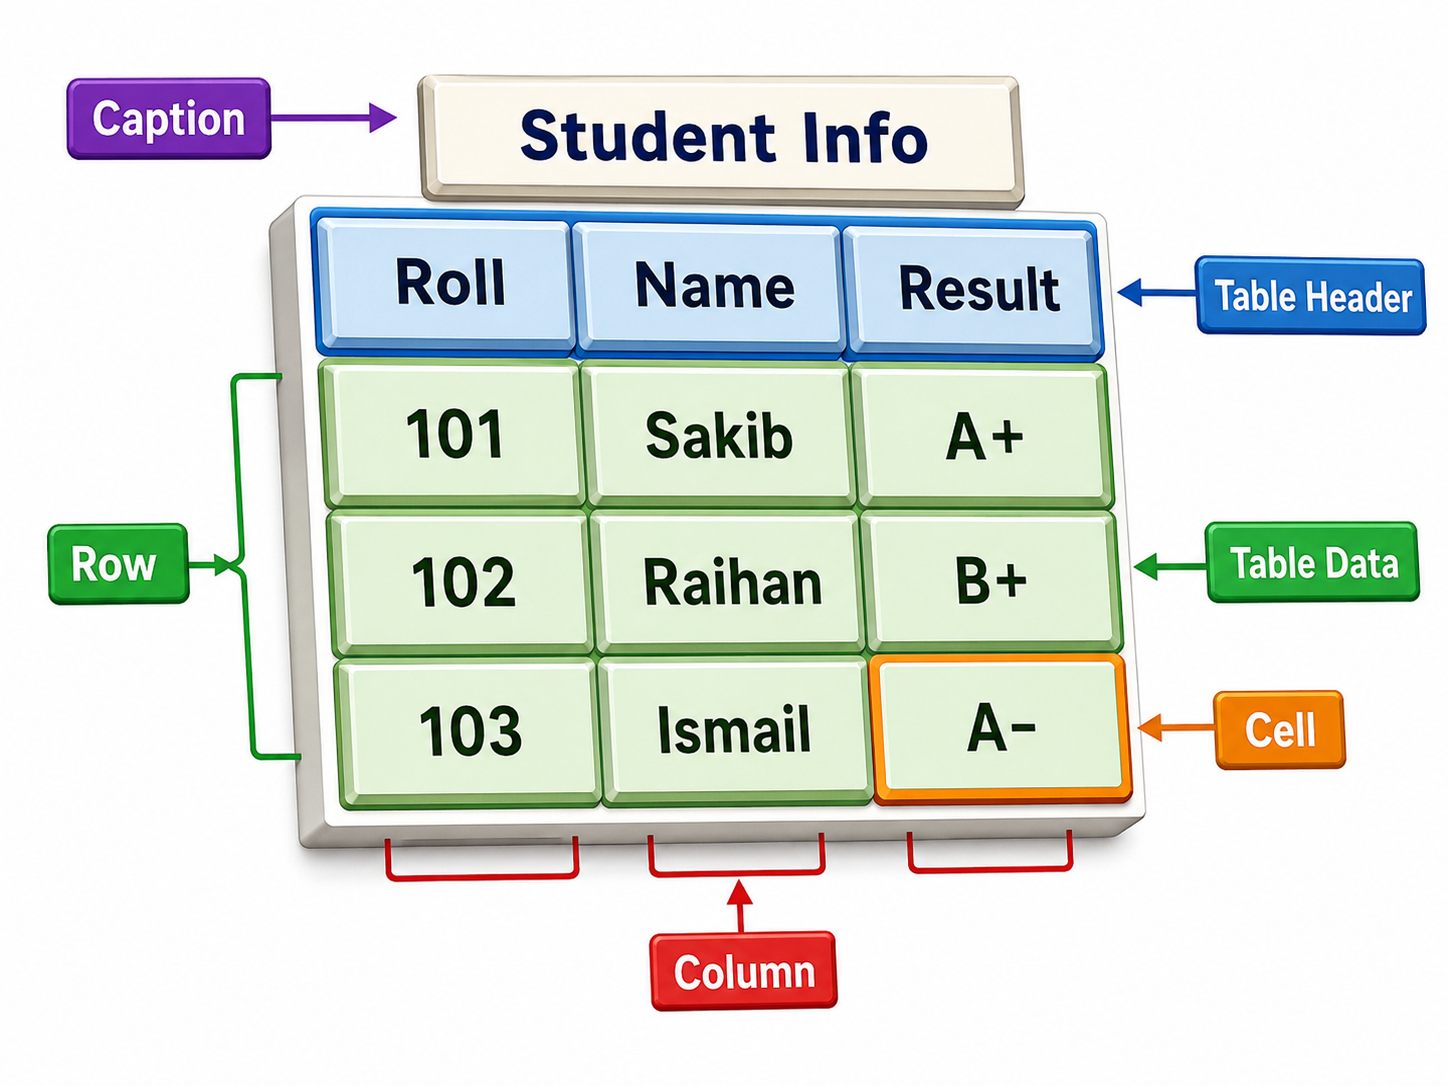
\includegraphics[width=0.98\linewidth,height=0.20\textheight,keepaspectratio]{chapters/Chapter04/topics/images/3d_row_column_cell.png}%
}{%
\fbox{\parbox{0.88\linewidth}{\centering\scriptsize চিত্র পাওয়া যায়নি}}%
}
\par\vspace{1pt}
{\scriptsize\captionof{figure}{HTML table-এর row, column ও cell}}
\end{minipage}
\end{examplebox}


\subsection{Table তৈরির প্রধান Tag}

\noindent
\begin{minipage}[t]{0.56\textwidth}
\vspace{0pt}
\begin{center}
\begin{tabular}{|p{0.22\linewidth}|p{0.24\linewidth}|p{0.34\linewidth}|}
\hline
\textbf{Tag} & \textbf{পূর্ণরূপ/অর্থ} & \textbf{কাজ} \\
\hline
\texttt{<table>} & Table & table শুরু ও শেষ করে \\
\hline
\texttt{<tr>} & Table Row & table-এর row বা সারি তৈরি করে \\
\hline
\texttt{<th>} & Table Header & heading cell তৈরি করে \\
\hline
\texttt{<td>} & Table Data & data cell তৈরি করে \\
\hline
\texttt{<caption>} & Caption & table-এর title বা শিরোনাম দেখায় \\
\hline
\end{tabular}
\end{center}
\textbf{চিত্র ব্যাখ্যা:}
চিত্রে table তৈরির প্রধান tagগুলোর সম্পর্ক দেখানো হয়েছে। \texttt{<table>} পুরো table, \texttt{<tr>} row, \texttt{<th>} heading cell এবং \texttt{<td>} data cell তৈরি করে।
\end{minipage}
\hfill
\begin{minipage}[t]{0.38\textwidth}
\vspace{0pt}
\centering
\IfFileExists{chapters/Chapter04/topics/images/3d_table_tags_map.png}{%
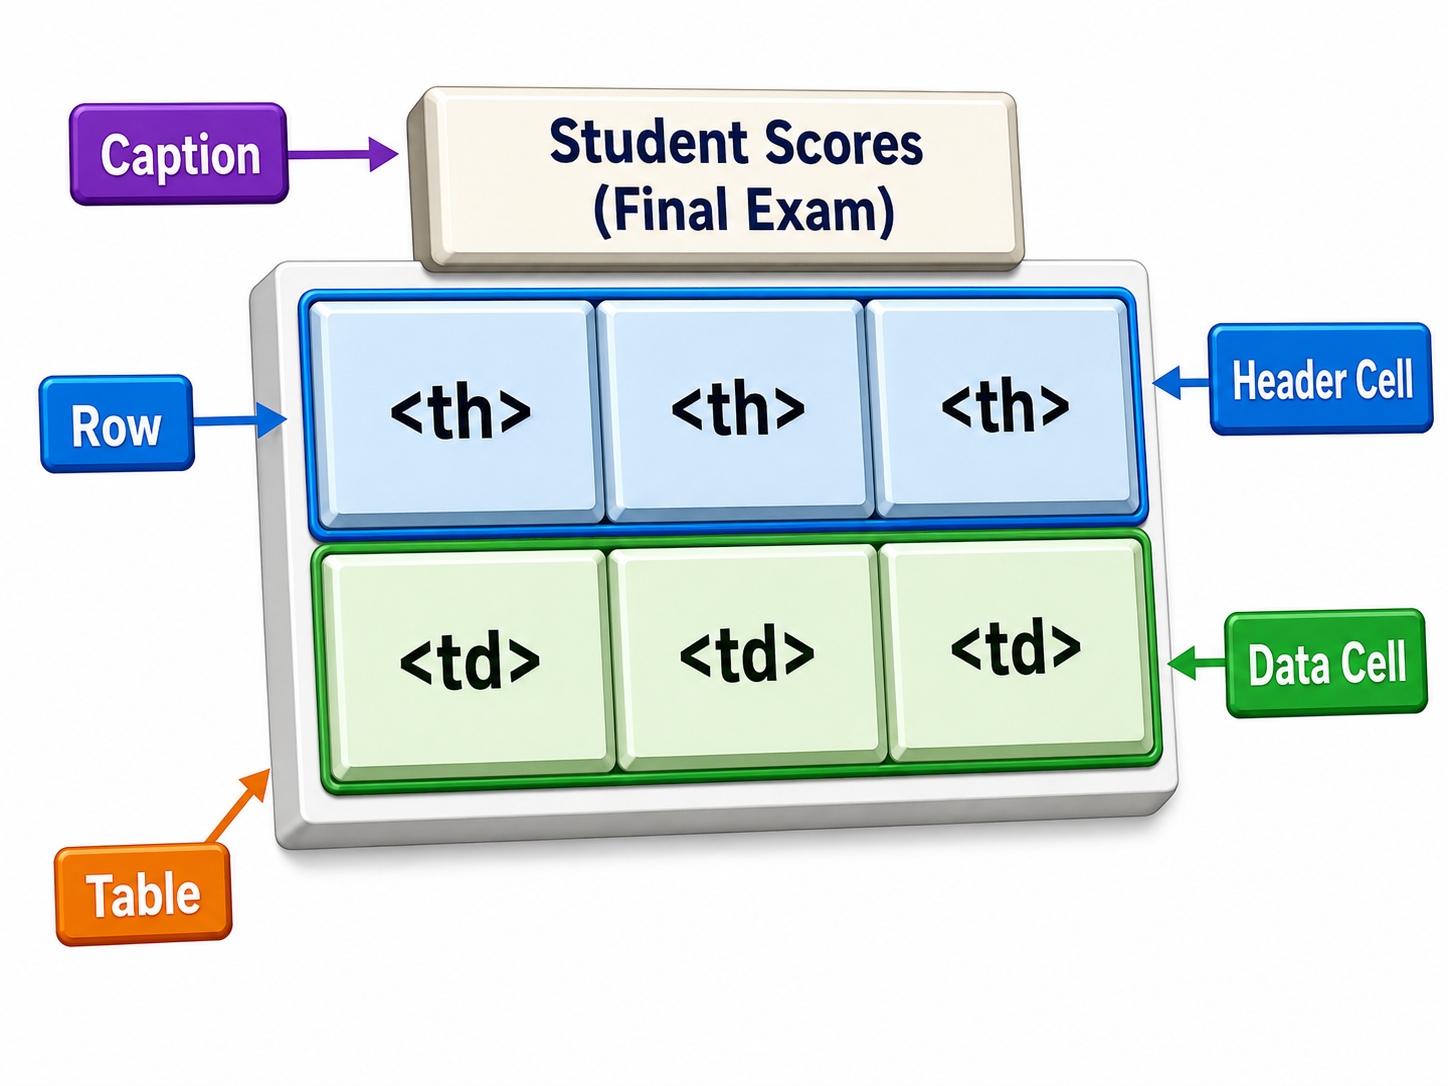
\includegraphics[width=0.98\linewidth,height=0.22\textheight,keepaspectratio]{chapters/Chapter04/topics/images/3d_table_tags_map.png}%
}{%
\fbox{\parbox{0.88\linewidth}{\centering\scriptsize চিত্র পাওয়া যায়নি}}%
}
\par\vspace{1pt}
{\scriptsize\captionof{figure}{table tag-এর কাজ}}
\end{minipage}


\subsection{\texttt{<table>} Tag}

\begin{definitionbox}{\texttt{<table>} tag}
HTML document-এ table বা ছক তৈরি করার জন্য ব্যবহৃত container tag হলো \texttt{<table>} tag।
\end{definitionbox}

Table-এর সব row ও cell এই tag-এর ভিতরে লেখা হয়।

\begin{examplebox}{কোড}
\begin{verbatim}
<!DOCTYPE html>
<html>
<head>
  <title>HTML Table Example</title>
</head>
<body>
  <table border="1" cellspacing="0" cellpadding="6">
    <tr>
      <td>Data</td>
    </tr>
  </table>
</body>
</html>
\end{verbatim}
\end{examplebox}

\subsection{\texttt{<tr>} Tag}

\begin{definitionbox}{\texttt{<tr>} tag}
HTML table-এর একটি row বা সারি তৈরি করার জন্য \texttt{<tr>} tag ব্যবহার করা হয়।
\end{definitionbox}

প্রতিটি \texttt{<tr>} tag-এর ভিতরে এক বা একাধিক \texttt{<th>} অথবা \texttt{<td>} লেখা হয়।

\begin{examplebox}{কোড}
\begin{verbatim}
<!DOCTYPE html>
<html>
<head>
  <title>Table Row Example</title>
</head>
<body>
  <table border="1" cellspacing="0" cellpadding="6">
    <tr>
      <td>Data 1</td>
      <td>Data 2</td>
    </tr>
  </table>
</body>
</html>
\end{verbatim}
\end{examplebox}

\subsection{\texttt{<th>} Tag}

\begin{definitionbox}{\texttt{<th>} tag}
HTML table-এর heading cell তৈরি করার জন্য ব্যবহৃত tag হলো \texttt{<th>} tag।
\end{definitionbox}

Browser সাধারণত \texttt{<th>} tag-এর text bold ও center aligned করে দেখায়।

\begin{examplebox}{কোড}
\begin{verbatim}
<!DOCTYPE html>
<html>
<head>
  <title>Table Header Example</title>
</head>
<body>
  <table border="1" cellspacing="0" cellpadding="6">
    <tr>
      <th>Name</th>
      <th>Roll</th>
    </tr>
  </table>
</body>
</html>
\end{verbatim}
\end{examplebox}

\subsection{\texttt{<td>} Tag}

\begin{definitionbox}{\texttt{<td>} tag}
HTML table-এর data cell বা তথ্যের ঘর তৈরি করার জন্য ব্যবহৃত tag হলো \texttt{<td>} tag।
\end{definitionbox}

\begin{examplebox}{কোড}
\begin{verbatim}
<!DOCTYPE html>
<html>
<head>
  <title>Table Data Example</title>
</head>
<body>
  <table border="1" cellspacing="0" cellpadding="6">
    <tr>
      <td>Rafi</td>
      <td>101</td>
    </tr>
  </table>
</body>
</html>
\end{verbatim}
\end{examplebox}

\subsection{Basic Table Syntax}

\begin{examplebox}{কোড}
\begin{verbatim}
<!DOCTYPE html>
<html>
<head>
  <title>HTML Table Example</title>
</head>
<body>
<table>
  <tr>
    <th>Heading 1</th>
    <th>Heading 2</th>
  </tr>
  <tr>
    <td>Data 1</td>
    <td>Data 2</td>
  </tr>
</table>
</body>
</html>
\end{verbatim}
\end{examplebox}

\begin{keypointbox}{Structure মনে রাখো}
\texttt{<table>} পুরো table তৈরি করে, \texttt{<tr>} একটি row তৈরি করে, \texttt{<th>} heading cell তৈরি করে এবং \texttt{<td>} data cell তৈরি করে।
\end{keypointbox}

\subsection{Table Code লেখার Logical Structure}

HTML table লেখার সময় browser উপর থেকে নিচে row-by-row code পড়ে। তাই code লেখার সময় কোনো cell আগে বা পরে লিখলে visual output বদলে যেতে পারে। একটি row শুরু করতে \texttt{<tr>} লিখতে হয় এবং সেই row-এর যতগুলো cell আছে সেগুলো \texttt{<th>} অথবা \texttt{<td>} দিয়ে একই \texttt{<tr>} tag-এর ভিতরে লিখতে হয়।

\begin{keypointbox}{মনে রাখার নিয়ম}
Table-এর ভিতরে সরাসরি text লেখা উচিত নয়। Table-এর content সাধারণত cell-এর ভিতরে থাকে। তাই correct structure হলো:
\texttt{<table>} $\rightarrow$ \texttt{<tr>} $\rightarrow$ \texttt{<th>} বা \texttt{<td>} $\rightarrow$ content।
\end{keypointbox}

\begin{center}
\begin{tabular}{|p{0.24\textwidth}|p{0.58\textwidth}|}
\hline
\textbf{ধাপ} & \textbf{কাজ} \\
\hline
১ & \texttt{<table>} দিয়ে table শুরু করা \\
\hline
২ & প্রতিটি row-এর জন্য \texttt{<tr>} লেখা \\
\hline
৩ & heading হলে \texttt{<th>}, data হলে \texttt{<td>} লেখা \\
\hline
৪ & সব opened tag ঠিকভাবে close করা \\
\hline
\end{tabular}
\end{center}

\subsection{Simple Table Example}

\begin{examplebox}{কোড}
\begin{verbatim}
<!DOCTYPE html>
<html>
<head>
  <title>Simple Table</title>
</head>
<body>
  <table border="1">
    <tr>
      <th>Roll</th>
      <th>Name</th>
      <th>GPA</th>
    </tr>
    <tr>
      <td>101</td>
      <td>Rafi</td>
      <td>5.00</td>
    </tr>
    <tr>
      <td>102</td>
      <td>Sakib</td>
      <td>4.75</td>
    </tr>
  </table>
</body>
</html>
\end{verbatim}
\end{examplebox}

\begin{examplebox}{Output ধারণা}
\begin{center}
\begin{tabular}{|c|c|c|}
\hline
\textbf{Roll} & \textbf{Name} & \textbf{GPA} \\
\hline
101 & Rafi & 5.00 \\
\hline
102 & Sakib & 4.75 \\
\hline
\end{tabular}
\end{center}
\end{examplebox}

\begin{boardbox}{কোড বিশ্লেষণ}
উপরের code-এ প্রথম \texttt{<tr>} হলো heading row। সেখানে Roll, Name, GPA--এই তিনটি heading cell আছে, তাই \texttt{<th>} ব্যবহার করা হয়েছে। পরের দুইটি row data row, তাই সেখানে \texttt{<td>} ব্যবহার করা হয়েছে। \texttt{border="1"} দেওয়ার কারণে table-এর রেখা দেখা যাচ্ছে।
\end{boardbox}

\subsection{Table Design করার আগে কী ভাববে?}

চিত্র দেখে বা question পড়ে table code লেখার আগে সরাসরি code শুরু না করে কয়েকটি বিষয় ঠিক করতে হয়। এতে ভুল কম হয় এবং \texttt{rowspan}/\texttt{colspan} সহজে বোঝা যায়।

\begin{enumerate}
\item Table-এর title বা caption আছে কি না দেখবে।
\item মোট কয়টি visible column আছে তা গুনবে।
\item মোট কয়টি row আছে তা গুনবে।
\item কোন cell heading আর কোন cell data তা আলাদা করবে।
\item কোনো cell একাধিক column জুড়ে আছে কি না দেখবে।
\item কোনো cell একাধিক row জুড়ে আছে কি না দেখবে।
\item cell-এর ভিতরে text, image, link, list বা nested table আছে কি না দেখবে।
\end{enumerate}

\begin{keypointbox}{পরীক্ষার কৌশল}
কোনো figure জটিল মনে হলে প্রথমে pencil দিয়ে row line ও column line আলাদা করে ভাববে। এরপর merged cell বাদ দিয়ে base grid ধরবে। Base grid বুঝলে \texttt{rowspan} ও \texttt{colspan} বসানো সহজ হয়।
\end{keypointbox}

\subsection{Table Attribute}

PDF-এ table তৈরি করার সময় কয়েকটি attribute বারবার ব্যবহার করা হয়েছে। HSC practical exam-এ এগুলো গুরুত্বপূর্ণ। Table-level attribute যেমন \texttt{border}, \texttt{width}, \texttt{align}, \texttt{cellspacing}, \texttt{cellpadding} পুরো table-এর appearance নিয়ন্ত্রণ করে। আবার cell-level attribute যেমন \texttt{align}, \texttt{valign}, \texttt{bgcolor}, \texttt{rowspan}, \texttt{colspan}, \texttt{width}, \texttt{height} নির্দিষ্ট \texttt{<td>} বা \texttt{<th>} cell-এর আচরণ নিয়ন্ত্রণ করে।

\begin{center}
\begin{tabular}{|p{0.20\textwidth}|p{0.42\textwidth}|p{0.25\textwidth}|}
\hline
\textbf{Attribute} & \textbf{কাজ} & \textbf{Example} \\
\hline
\texttt{border} & table ও cell-এর চারপাশে রেখা দেখায় & \texttt{border="1"} \\
\hline
\texttt{width} & table বা cell-এর প্রস্থ pixel/percentage-এ নির্ধারণ করে & \texttt{width="400"} \\
\hline
\texttt{align} & table বা cell-এর left/right/center position নির্ধারণ করে & \texttt{align="center"} \\
\hline
\texttt{cellspacing} & cell থেকে cell-এর মাঝের বাইরের gap নির্ধারণ করে & \texttt{cellspacing="0"} \\
\hline
\texttt{cellpadding} & cell content ও border-এর মাঝের ভিতরের gap নির্ধারণ করে & \texttt{cellpadding="5"} \\
\hline
\texttt{bgcolor} & table/cell-এর background color দেয় & \texttt{bgcolor="yellow"} \\
\hline
\end{tabular}
\end{center}

\begin{keypointbox}{PDF থেকে গুরুত্বপূর্ণ point}
\texttt{border} attribute না দিলে table-এর রেখা সবসময় দেখা যায় না। বইয়ের example-গুলোতে single-line border দেখাতে বেশিরভাগ সময় \texttt{border="1"}-এর সাথে \texttt{cellspacing="0"} ব্যবহার করা হয়েছে। \texttt{width="75\%"} দিলে table parent area-এর 75\% জায়গা নেয়, আর \texttt{width="400"} বা \texttt{width="400px"} দিলে fixed pixel width বোঝায়।
\end{keypointbox}

\conceptimagerow{chapters/Chapter04/topics/images/3d_table_attributes.png}{
\begin{keypointbox}{চিত্র ব্যাখ্যা}
চিত্রে \texttt{border}, \texttt{width}, \texttt{align}, \texttt{bgcolor}, \texttt{cellspacing} ও \texttt{cellpadding} attribute table-এর appearance কীভাবে বদলায় তা দেখানো হয়েছে।
\end{keypointbox}
}{table attribute-এর প্রভাব}


\subsection{\texttt{border} Attribute}

\begin{definitionbox}{\texttt{border} attribute}
HTML table-এর চারপাশে ও cell-এর চারপাশে border প্রদর্শনের জন্য \texttt{border} attribute ব্যবহার করা হয়।
\end{definitionbox}

\begin{examplebox}{কোড}
\begin{verbatim}
<!DOCTYPE html>
<html>
<head>
  <title>HTML Table Example</title>
</head>
<body>
<table border="1">
  <tr>
    <th>Subject</th>
    <th>Mark</th>
  </tr>
  <tr>
    <td>ICT</td>
    <td>95</td>
  </tr>
</table>
</body>
</html>
\end{verbatim}
\end{examplebox}

\begin{boardbox}{পরীক্ষায় মনে রাখবে}
HSC practical code-এ table-এর রেখা দেখাতে সাধারণত \texttt{border="1"} ব্যবহার করা হয়। Border না দিলে browser table-এর cell boundary সবসময় স্পষ্টভাবে দেখায় না। Border-এর মান 1, 2, 3 ইত্যাদি হলে রেখার thickness বাড়ে; তবে neat table-এর জন্য \texttt{border="1"} এবং \texttt{cellspacing="0"} সবচেয়ে বেশি ব্যবহৃত।
\end{boardbox}

\subsection{\texttt{width} Attribute}

Table বা cell-এর প্রস্থ নির্ধারণ করতে \texttt{width} attribute ব্যবহার করা যায়। Width pixel বা percentage আকারে দেওয়া যায়।

Pixel width fixed size দেয়, তাই \texttt{width="400"} দিলে table প্রায় 400 pixel জায়গা নেবে। Percentage width flexible; \texttt{width="75\%"} দিলে browser window বা parent container-এর 75\% জায়গা ব্যবহার করবে। Cell-এর \texttt{width} দিলে নির্দিষ্ট column তুলনামূলক বড় বা ছোট করা যায়।

\begin{examplebox}{কোড}
\begin{verbatim}
<!DOCTYPE html>
<html>
<head>
  <title>HTML Table Example</title>
</head>
<body>
<table border="1" width="400">
  <tr>
    <th>Name</th>
    <th>GPA</th>
  </tr>
  <tr>
    <td>Rafi</td>
    <td>5.00</td>
  </tr>
</table>
</body>
</html>
\end{verbatim}
\end{examplebox}

\begin{examplebox}{Percentage Width}
\begin{verbatim}
<!DOCTYPE html>
<html>
<head>
  <title>HTML Table Example</title>
</head>
<body>
  <table border="1" width="75%">
    <tr>
      <th>Name</th>
      <th>GPA</th>
    </tr>
    <tr>
      <td>Rafi</td>
      <td>5.00</td>
    </tr>
  </table>
</body>
</html>
\end{verbatim}
এখানে table browser window বা parent area-এর 75\% জায়গা নেবে।
\end{examplebox}

\subsection{\texttt{align} Attribute}

Table, row বা cell-এর content left, right বা center-এ রাখতে \texttt{align} attribute ব্যবহার করা হয়।

\texttt{<table align="center">} লিখলে পুরো table page-এর মাঝখানে চলে আসে। কিন্তু \texttt{<td align="center">} লিখলে শুধু ওই cell-এর content মাঝখানে থাকে। তাই table-এর position এবং cell-এর ভিতরের text alignment আলাদা বিষয়।

\begin{examplebox}{কোড}
\begin{verbatim}
<!DOCTYPE html>
<html>
<head>
  <title>Align Example</title>
</head>
<body>
  <table border="1" cellspacing="0" cellpadding="6">
    <tr>
      <td align="center">ICT</td>
    </tr>
  </table>
</body>
</html>
\end{verbatim}
\end{examplebox}

\begin{center}
\begin{tabular}{|p{0.25\textwidth}|p{0.55\textwidth}|}
\hline
\textbf{Value} & \textbf{কাজ} \\
\hline
\texttt{left} & বামে রাখে \\
\hline
\texttt{center} & মাঝখানে রাখে \\
\hline
\texttt{right} & ডানে রাখে \\
\hline
\end{tabular}
\end{center}

\subsection{\texttt{valign} Attribute}

Cell-এর ভিতরের content vertical direction-এ কোথায় থাকবে তা নির্ধারণ করতে \texttt{valign} attribute ব্যবহার করা যায়।

কোনো cell-এর height বেশি হলে content উপরে, মাঝখানে বা নিচে রাখা দরকার হতে পারে। শুধু \texttt{<br>} দিয়ে content নিচে নামানো যায়, কিন্তু board-style পরিষ্কার code-এর জন্য \texttt{valign="top"}, \texttt{valign="middle"} বা \texttt{valign="bottom"} ব্যবহার করা ভালো।

\begin{center}
\begin{tabular}{|p{0.25\textwidth}|p{0.55\textwidth}|}
\hline
\textbf{Value} & \textbf{কাজ} \\
\hline
\texttt{top} & cell-এর উপরে রাখে \\
\hline
\texttt{middle} & cell-এর মাঝখানে রাখে \\
\hline
\texttt{bottom} & cell-এর নিচে রাখে \\
\hline
\end{tabular}
\end{center}

\conceptimagerow{chapters/Chapter04/topics/images/3d_align_valign.png}{
\begin{keypointbox}{চিত্র ব্যাখ্যা}
চিত্রে horizontal alignment এবং vertical alignment-এর পার্থক্য দেখানো হয়েছে। \texttt{align} left/center/right position নিয়ন্ত্রণ করে এবং \texttt{valign} top/middle/bottom position নিয়ন্ত্রণ করে।
\end{keypointbox}
}{horizontal alignment ও vertical alignment}


\subsection{\texttt{cellspacing} Attribute}

\begin{definitionbox}{\texttt{cellspacing} attribute}
Table-এর এক cell-এর border থেকে পাশের cell-এর border পর্যন্ত ফাঁকা জায়গা নির্ধারণ করতে \texttt{cellspacing} attribute ব্যবহার করা হয়।
\end{definitionbox}

\begin{examplebox}{কোড}
\begin{verbatim}
<!DOCTYPE html>
<html>
<head>
  <title>HTML Table Example</title>
</head>
<body>
<table border="1" cellspacing="0">
  <tr>
    <th>Name</th>
    <th>Class</th>
  </tr>
  <tr>
    <td>Rafi</td>
    <td>XI</td>
  </tr>
</table>
</body>
</html>
\end{verbatim}
\end{examplebox}

\begin{keypointbox}{সহজ কথা}
Browser অনেক সময় default হিসেবে cell-এর মাঝে সামান্য gap রাখে। \texttt{cellspacing="0"} দিলে cell-এর মাঝখানের gap কমে যায় বা borderগুলো একসাথে লেগে থাকে। আবার \texttt{cellspacing="10"} দিলে দুই cell-এর border-এর মাঝে 10 pixel দূরত্ব তৈরি হয়।
\end{keypointbox}

\subsection{\texttt{cellpadding} Attribute}

\begin{definitionbox}{\texttt{cellpadding} attribute}
Table cell-এর content এবং cell border-এর মাঝখানের ভিতরের ফাঁকা জায়গা নির্ধারণ করতে \texttt{cellpadding} attribute ব্যবহার করা হয়।
\end{definitionbox}

\begin{examplebox}{কোড}
\begin{verbatim}
<!DOCTYPE html>
<html>
<head>
  <title>HTML Table Example</title>
</head>
<body>
<table border="1" cellpadding="10">
  <tr>
    <th>Subject</th>
    <th>GPA</th>
  </tr>
  <tr>
    <td>Bangla</td>
    <td>5.00</td>
  </tr>
</table>
</body>
</html>
\end{verbatim}
\end{examplebox}

\begin{boardbox}{MCQ point}
\texttt{cellpadding="5"} অর্থ cell content এবং cell border-এর মাঝখানে 5 pixel ভিতরের ফাঁকা জায়গা রাখা। অনেক browser-এ default cellpadding খুব কম থাকে; তাই text border-এর সাথে লেগে গেলে \texttt{cellpadding} বাড়ালে table পড়তে সহজ হয়।
\end{boardbox}

\subsection{\texttt{cellspacing} ও \texttt{cellpadding}-এর পার্থক্য}

\begin{center}
\begin{tabular}{|p{0.18\textwidth}|p{0.34\textwidth}|p{0.34\textwidth}|}
\hline
\textbf{বিষয়} & \textbf{\texttt{cellspacing}} & \textbf{\texttt{cellpadding}} \\
\hline
কাজ & cell থেকে cell-এর মাঝের gap নির্ধারণ করে & cell content থেকে border-এর ভিতরের gap নির্ধারণ করে \\
\hline
অবস্থান & cell-এর বাইরে & cell-এর ভিতরে \\
\hline
Example & \texttt{cellspacing="0"} & \texttt{cellpadding="5"} \\
\hline
প্রভাব & border-এর মাঝের দূরত্ব কমায় বা বাড়ায় & content-এর চারপাশে space দেয় \\
\hline
\end{tabular}
\end{center}

\begin{center}
\IfFileExists{chapters/Chapter04/topics/images/3d_cellspacing_vs_cellpadding.png}{
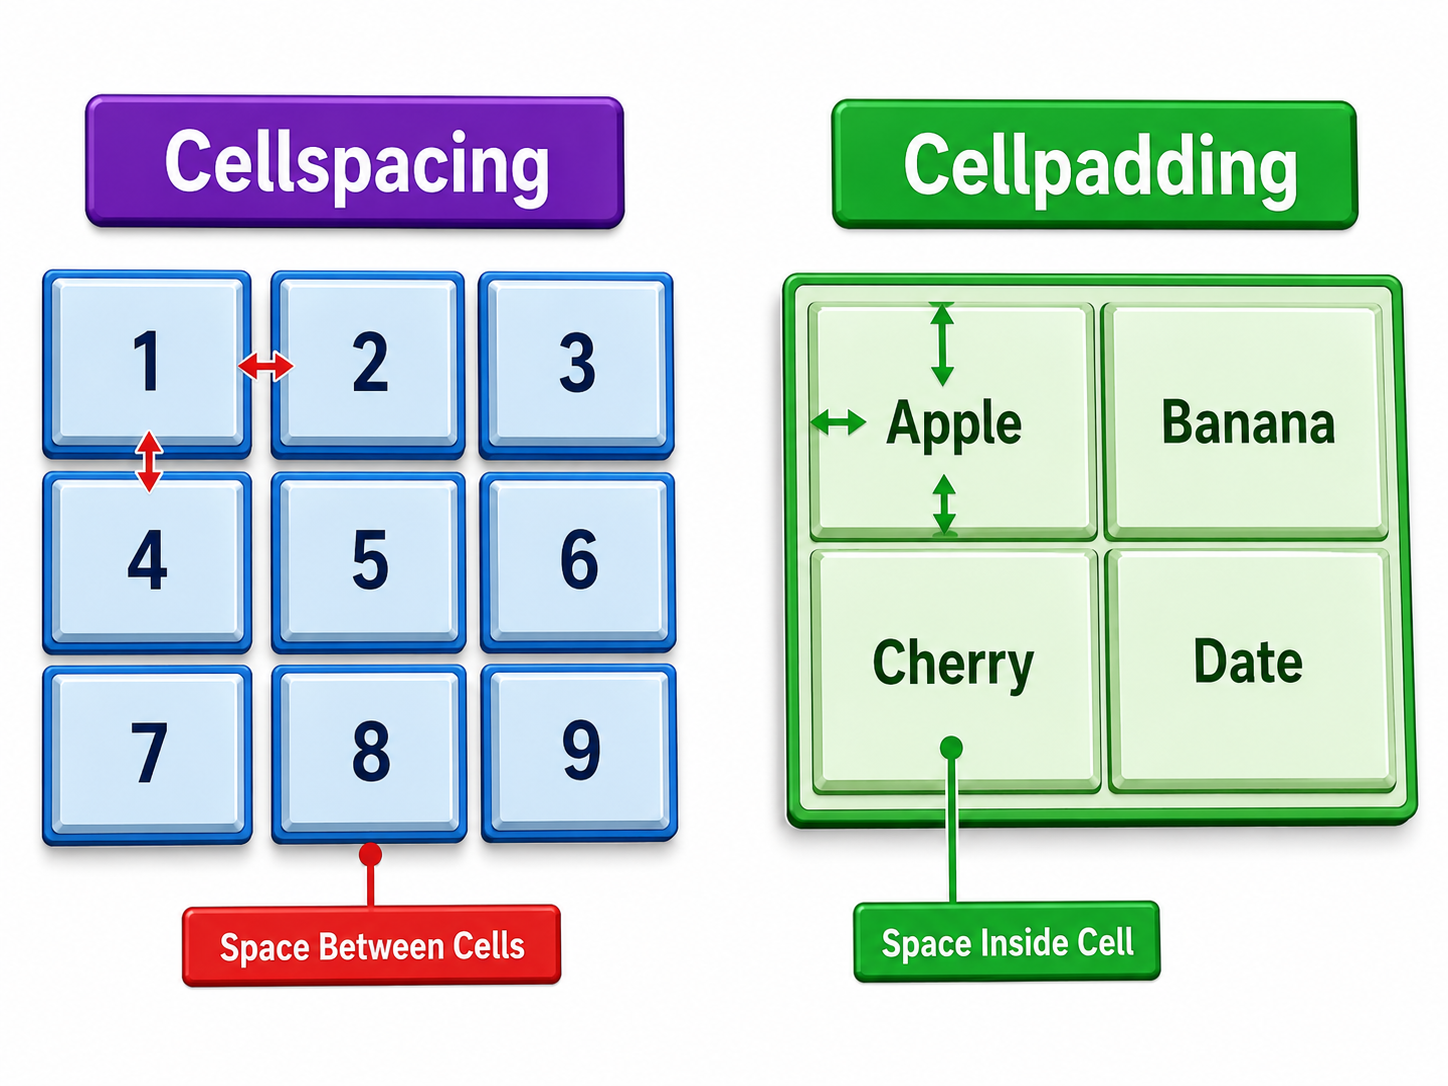
\includegraphics[width=0.95\linewidth,height=0.11\textheight,keepaspectratio]{chapters/Chapter04/topics/images/3d_cellspacing_vs_cellpadding.png}
}{
\fbox{\parbox{0.90\linewidth}{\centering\vspace{0.5cm}
\textbf{চিত্র}\\[4pt]
Left side: gap between two cell boxes labeled \texttt{cellspacing}. Right side: inner gap from content to cell wall labeled \texttt{cellpadding}.\\[4pt]
File: \texttt{chapters/Chapter04/topics/images/3d\_cellspacing\_vs\_cellpadding.png}
\vspace{0.5cm}}}
}
\captionof{figure}{cellspacing ও cellpadding-এর পার্থক্য}
\end{center}

\begin{keypointbox}{চিত্র ব্যাখ্যা}
চিত্রে \texttt{cellspacing} cell-এর মাঝের gap এবং \texttt{cellpadding} cell-এর ভিতরে content ও border-এর মাঝের gap তৈরি করে তা দেখানো হয়েছে।
\end{keypointbox}


\begin{keypointbox}{সহজ মনে রাখার উপায়}
Spacing মানে cell ও cell-এর মাঝে space। Padding মানে cell-এর ভিতরে content-এর চারপাশে space।
\end{keypointbox}

\subsection{\texttt{bgcolor} Attribute}

Table বা cell-এর background color দিতে \texttt{bgcolor} attribute ব্যবহার করা হয়।

\begin{examplebox}{কোড}
\begin{verbatim}
<!DOCTYPE html>
<html>
<head>
  <title>HTML Table Example</title>
</head>
<body>
<table border="1" bgcolor="yellow">
  <tr>
    <th>Name</th>
    <th>Class</th>
  </tr>
  <tr>
    <td>Rafi</td>
    <td>XI</td>
  </tr>
</table>
</body>
</html>
\end{verbatim}
\end{examplebox}

\subsection{\texttt{<td>} ও \texttt{<th>} Tag-এর Attribute}

Cell-এর উপর আলাদা control দেওয়ার জন্য \texttt{<td>} বা \texttt{<th>} tag-এর ভিতরে attribute ব্যবহার করা যায়।

PDF-এর table অংশে \texttt{<th>} ও \texttt{<td>} cell-এর জন্য আলাদা attribute দেখানো হয়েছে। একই table-এর সব cell একরকম নাও হতে পারে; কোনো cell center aligned, কোনো cell green background, কোনো cell বেশি wide, আবার কোনো cell একাধিক row বা column জুড়ে থাকতে পারে।

\begin{center}
\begin{tabular}{|p{0.18\textwidth}|p{0.46\textwidth}|p{0.25\textwidth}|}
\hline
\textbf{Attribute} & \textbf{কাজ} & \textbf{Example} \\
\hline
\texttt{align} & cell-এর text বাম/মাঝ/ডানে রাখে & \texttt{align="center"} \\
\hline
\texttt{valign} & cell-এর text top/middle/bottom রাখে & \texttt{valign="top"} \\
\hline
\texttt{bgcolor} & cell-এর background color দেয় & \texttt{bgcolor="green"} \\
\hline
\texttt{width} & cell-এর width নির্ধারণ করে & \texttt{width="150"} \\
\hline
\texttt{height} & cell-এর height নির্ধারণ করে & \texttt{height="60"} \\
\hline
\texttt{colspan} & cell-কে একাধিক column জুড়ে দেয় & \texttt{colspan="2"} \\
\hline
\texttt{rowspan} & cell-কে একাধিক row জুড়ে দেয় & \texttt{rowspan="3"} \\
\hline
\end{tabular}
\end{center}

\begin{keypointbox}{Color value}
\texttt{bgcolor} attribute-এ color name, hexadecimal value বা RGB ধরনের value ব্যবহার করা যায়। HSC practical-এ সাধারণত \texttt{yellow}, \texttt{green}, \texttt{silver} ধরনের color name বেশি দেখা যায়।
\end{keypointbox}

\subsection{\texttt{rowspan} ও \texttt{colspan}}

\begin{definitionbox}{\texttt{colspan}}
একটি cell-কে একাধিক column বা কলাম জুড়ে বিস্তৃত করার জন্য \texttt{colspan} attribute ব্যবহার করা হয়।
\end{definitionbox}

\begin{definitionbox}{\texttt{rowspan}}
একটি cell-কে একাধিক row বা সারি জুড়ে বিস্তৃত করার জন্য \texttt{rowspan} attribute ব্যবহার করা হয়।
\end{definitionbox}

\begin{examplebox}{\texttt{colspan} কোড}
\begin{verbatim}
<!DOCTYPE html>
<html>
<head>
  <title>HTML Table Example</title>
</head>
<body>
<table border="1">
  <tr>
    <th colspan="2">Student Info</th>
  </tr>
  <tr>
    <td>Roll</td>
    <td>101</td>
  </tr>
</table>
</body>
</html>
\end{verbatim}
\end{examplebox}

\begin{examplebox}{\texttt{rowspan} কোড}
\begin{verbatim}
<!DOCTYPE html>
<html>
<head>
  <title>HTML Table Example</title>
</head>
<body>
<table border="1">
  <tr>
    <th rowspan="2">Name</th>
    <td>Rafi</td>
  </tr>
  <tr>
    <td>Sakib</td>
  </tr>
</table>
</body>
</html>
\end{verbatim}
\end{examplebox}

\begin{center}
\IfFileExists{chapters/Chapter04/topics/images/3d_rowspan_colspan.png}{
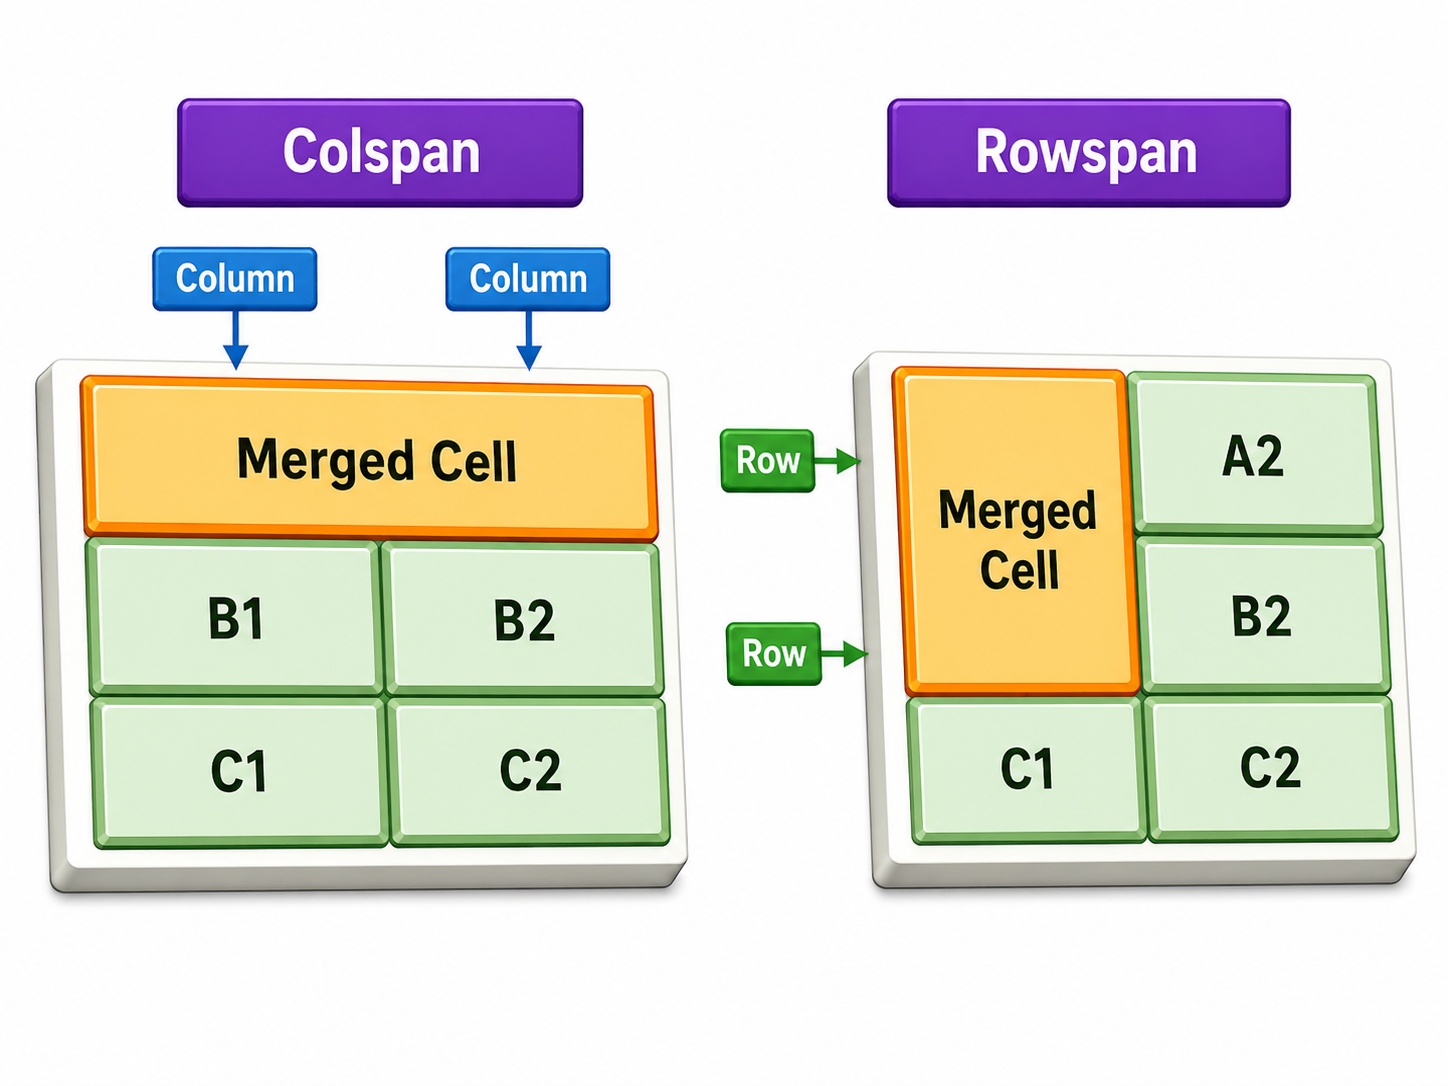
\includegraphics[width=0.95\linewidth,height=0.11\textheight,keepaspectratio]{chapters/Chapter04/topics/images/3d_rowspan_colspan.png}
}{
\fbox{\parbox{0.90\linewidth}{\centering\vspace{0.5cm}
\textbf{চিত্র}\\[4pt]
Two grids: one shows a wide block covering two columns labeled \texttt{colspan="2"}; another shows a tall block covering two rows labeled \texttt{rowspan="2"}.\\[4pt]
File: \texttt{chapters/Chapter04/topics/images/3d\_rowspan\_colspan.png}
\vspace{0.5cm}}}
}
\captionof{figure}{rowspan ও colspan দিয়ে cell merge}
\end{center}

\begin{keypointbox}{চিত্র ব্যাখ্যা}
চিত্রে \texttt{colspan} দিয়ে horizontal merge এবং \texttt{rowspan} দিয়ে vertical merge দেখানো হয়েছে। চিত্র দেখে code লেখার সময় merged cell আগে identify করতে হয়।
\end{keypointbox}


\begin{keypointbox}{Shortcut}
\texttt{colspan} = column span = পাশের দিকে merge।\\
\texttt{rowspan} = row span = নিচের দিকে merge।
\end{keypointbox}

\subsection{Merged Cell বুঝে Code লেখার নিয়ম}

Merged cell হলো এমন cell, যা একাধিক row বা column-এর জায়গা নেয়। Table চিত্র দেখে code লেখার সময় merged cell ভুল হলে পুরো table layout নষ্ট হয়ে যায়। তাই \texttt{rowspan} ও \texttt{colspan} ব্যবহার করার আগে base column সংখ্যা ঠিক করা দরকার।

\begin{boardbox}{\texttt{colspan} কখন ব্যবহার করবে}
যদি কোনো cell বাম থেকে ডানে একাধিক column-এর জায়গা নেয়, তখন \texttt{colspan} ব্যবহার করবে। যেমন, একটি title যদি table-এর তিনটি column জুড়ে থাকে, তাহলে code হবে \texttt{<th colspan="3">Title</th>}।
\end{boardbox}

\begin{boardbox}{\texttt{rowspan} কখন ব্যবহার করবে}
যদি কোনো cell উপর থেকে নিচে একাধিক row-এর জায়গা নেয়, তখন \texttt{rowspan} ব্যবহার করবে। যেমন, একটি group name যদি দুইটি section row-এর জন্য common হয়, তাহলে code হবে \texttt{<td rowspan="2">Science</td>}।
\end{boardbox}

\begin{keypointbox}{Merged cell-এর কারণে cell count কমে যায়}
যে row-তে \texttt{colspan} বা \texttt{rowspan} ব্যবহার করা হয়, সেই row-তে আলাদা cell কম লিখতে হয়। কারণ merged cell নিজেই একাধিক cell-এর জায়গা দখল করে। এটাই beginners-দের সবচেয়ে সাধারণ ভুল।
\end{keypointbox}

\subsection{Empty Cell এবং \texttt{\&nbsp;}}

Table-এর কোনো cell খালি রাখতে চাইলে অনেক সময় browser cell-এর border ঠিকভাবে দেখাতে সমস্যা করতে পারে। তাই খালি cell-এ non-breaking space বা \texttt{\&nbsp;} ব্যবহার করা হয়।

খালি cell রাখা দরকার হলে শুধু blank space না দিয়ে \texttt{\&nbsp;} লেখা ভালো, কারণ এটি একটি invisible character হিসেবে কাজ করে। ফলে cell-এর height, width এবং border ঠিক থাকে। Board practical-এ empty cell দেখলে \texttt{<td>\&nbsp;</td>} লিখলে layout বেশি নির্ভরযোগ্য হয়। পুরনো বইয়ের example-এ খালি cell দেখাতে অনেক সময় \texttt{<br>} ব্যবহারও দেখা যায়, তবে পরীক্ষায় পরিষ্কারভাবে empty cell বোঝাতে \texttt{\&nbsp;} বেশি নির্ভরযোগ্য।

\begin{examplebox}{কোড}
\begin{verbatim}
<!DOCTYPE html>
<html>
<head>
  <title>Empty Cell Example</title>
</head>
<body>
  <table border="1" cellspacing="0" cellpadding="6">
    <tr>
      <th>Header 1</th>
      <th>Header 2</th>
    </tr>
    <tr>
      <td>Data</td>
      <td>&nbsp;</td>
    </tr>
  </table>
</body>
</html>
\end{verbatim}
\end{examplebox}

\conceptwrapimage{chapters/Chapter04/topics/images/3d_empty_cell_nbsp.png}
{চিত্রে empty cell দৃশ্যমান রাখতে \texttt{\&nbsp;} ব্যবহারের ধারণা দেখানো হয়েছে। খালি cell collapse বা অস্পষ্ট হলে non-breaking space ব্যবহার করা যায়।}
{খালি cell-এ \texttt{\&nbsp;} ব্যবহার}


\subsection{\texttt{<caption>} Tag}

\begin{definitionbox}{\texttt{<caption>} tag}
HTML table-এর শিরোনাম বা title প্রদর্শনের জন্য \texttt{<caption>} tag ব্যবহার করা হয়।
\end{definitionbox}

\texttt{<caption>} tag সবসময় \texttt{<table>} tag-এর ভিতরে এবং প্রথম row-এর আগে লেখা উচিত। এতে browser সাধারণত table-এর উপরে title দেখায়। Result sheet, routine, admission list বা product table-এর মতো table-এ caption দিলে table-এর উদ্দেশ্য দ্রুত বোঝা যায়। পুরনো HSC-style code-এ caption-এর position বোঝাতে \texttt{align="bottom"} ধরনের legacy attribute দেখা যেতে পারে, তবে modern HTML-এ caption position CSS দিয়ে নিয়ন্ত্রণ করা ভালো।

\begin{examplebox}{কোড}
\begin{verbatim}
<!DOCTYPE html>
<html>
<head>
  <title>Caption Example</title>
</head>
<body>
  <table border="1" cellspacing="0" cellpadding="6">
    <caption>Student Information</caption>
    <tr>
      <th>Roll</th>
      <th>Name</th>
      <th>Result</th>
    </tr>
    <tr>
      <td>101</td>
      <td>Sakib</td>
      <td>A+</td>
    </tr>
  </table>
</body>
</html>
\end{verbatim}
\end{examplebox}

\conceptwrapimage{chapters/Chapter04/topics/images/3d_caption.png}
{চিত্রে table-এর উপরে caption/title দেখানো হয়েছে। HTML-এ \texttt{<caption>} tag table-এর title লিখতে ব্যবহৃত হয়।}
{table caption}


\subsection{\texttt{colgroup} Tag}

\begin{definitionbox}{\texttt{<colgroup>} tag}
Table-এর এক বা একাধিক column-এর জন্য একসাথে style বা property নির্ধারণ করতে \texttt{<colgroup>} tag ব্যবহার করা হয়।
\end{definitionbox}

\texttt{colgroup} ব্যবহার করলে কোনো নির্দিষ্ট column বা column group-কে আলাদা color/style দেওয়া যায়। এটি table-এর row শুরু হওয়ার আগে লেখা হয়, কারণ column style আগে ঠিক করে তারপর row data বসানো হয়।

একই ধরনের একাধিক column একসাথে style করতে \texttt{<col span="2">} ব্যবহার করা যায়। যেমন প্রথম দুই column এক color এবং পরের দুই column আরেক color করতে চাইলে \texttt{span} attribute helpful। প্রতিটি column আলাদা style চাইলে আলাদা আলাদা \texttt{<col>} tag লেখা হয়।

\begin{examplebox}{কোড}
\begin{verbatim}
<!DOCTYPE html>
<html>
<head>
  <title>Column Group Example</title>
</head>
<body>
<table border="1">
  <colgroup>
    <col style="background-color: yellow">
    <col style="background-color: lightgreen">
  </colgroup>
  <tr>
    <th>Title</th>
    <th>Author</th>
  </tr>
  <tr>
    <td>ICT HSC</td>
    <td>M. Hakim</td>
  </tr>
</table>
</body>
</html>
\end{verbatim}
\end{examplebox}

\conceptwrapimage{chapters/Chapter04/topics/images/3d_colgroup.png}
{চিত্রে \texttt{<colgroup>} ব্যবহার করে নির্দিষ্ট column group-এ style দেওয়ার ধারণা দেখানো হয়েছে। এতে একাধিক column একসাথে color/style করা যায়।}
{colgroup দিয়ে column style}


\subsection{Table-এর ভিতরে Formatting, Link, Image ও List}

Table cell-এর ভিতরে শুধু text নয়, HTML-এর অন্য element-ও রাখা যায়। PDF-এর table discussion-এ cell-এর ভিতরে text, image, photograph, list, form, horizontal line, hyperlink এবং আরেকটি table রাখার ধারণা আছে। তাই table ব্যবহার করে result sheet-এর সাথে photo, product list-এর সাথে buy link, course plan-এর সাথে ordered list বা nested information দেখানো সম্ভব।

\begin{keypointbox}{Cell-এর ভিতরে content রাখার নিয়ম}
Cell-এর ভিতরে content রাখতে হলে content অবশ্যই \texttt{<td>} বা \texttt{<th>} tag-এর opening ও closing tag-এর মাঝখানে লিখতে হবে। যেমন image বসাতে \texttt{<td><img src="photo.jpg"></td>} এবং link বসাতে \texttt{<td><a href="page.html">Open</a></td>} লিখতে হবে।
\end{keypointbox}

\begin{center}
\begin{tabular}{|p{0.22\textwidth}|p{0.50\textwidth}|p{0.18\textwidth}|}
\hline
\textbf{Content type} & \textbf{Cell-এর ভিতরে code idea} & \textbf{Tag} \\
\hline
Text & \texttt{<td>Rafi</td>} & \texttt{<td>} \\
\hline
Image & \texttt{<td><img src="a.jpg"></td>} & \texttt{<img>} \\
\hline
Link & \texttt{<td><a href="a.html">Open</a></td>} & \texttt{<a>} \\
\hline
List & \texttt{<td><ol>...</ol></td>} & \texttt{<ol>}, \texttt{<li>} \\
\hline
Horizontal line & \texttt{<td><hr></td>} & \texttt{<hr>} \\
\hline
Form control & \texttt{<td><input type="text"></td>} & \texttt{<input>} \\
\hline
Nested table & \texttt{<td><table>...</table></td>} & \texttt{<table>} \\
\hline
\end{tabular}
\end{center}

\subsubsection{Formatting Text}

\begin{examplebox}{কোড}
\begin{verbatim}
<!DOCTYPE html>
<html>
<head>
  <title>Cell Formatting Example</title>
</head>
<body>
  <table border="1" cellspacing="0" cellpadding="6">
    <tr>
      <td><b>ICT</b></td>
      <td><u>HSC</u></td>
      <td><i>Book</i></td>
    </tr>
  </table>
</body>
</html>
\end{verbatim}
\end{examplebox}

\subsubsection{Hyperlink}

\begin{examplebox}{কোড}
\begin{verbatim}
<!DOCTYPE html>
<html>
<head>
  <title>Table Link Example</title>
</head>
<body>
  <table border="1" cellspacing="0" cellpadding="6">
    <tr>
      <td>
        <a href="https://www.educationboard.gov.bd">Education Board</a>
      </td>
    </tr>
  </table>
</body>
</html>
\end{verbatim}
\end{examplebox}

\subsubsection{Image}

\begin{examplebox}{কোড}
\begin{verbatim}
<!DOCTYPE html>
<html>
<head>
  <title>Table Image Example</title>
</head>
<body>
  <table border="1" cellspacing="0" cellpadding="6">
    <tr>
      <td>
        <img src="photo.jpg" width="100" height="80" alt="Photo">
      </td>
    </tr>
  </table>
</body>
</html>
\end{verbatim}
\end{examplebox}

\subsubsection{List}

\begin{center}
\IfFileExists{chapters/Chapter04/topics/images/3d_content_inside_cell.png}{
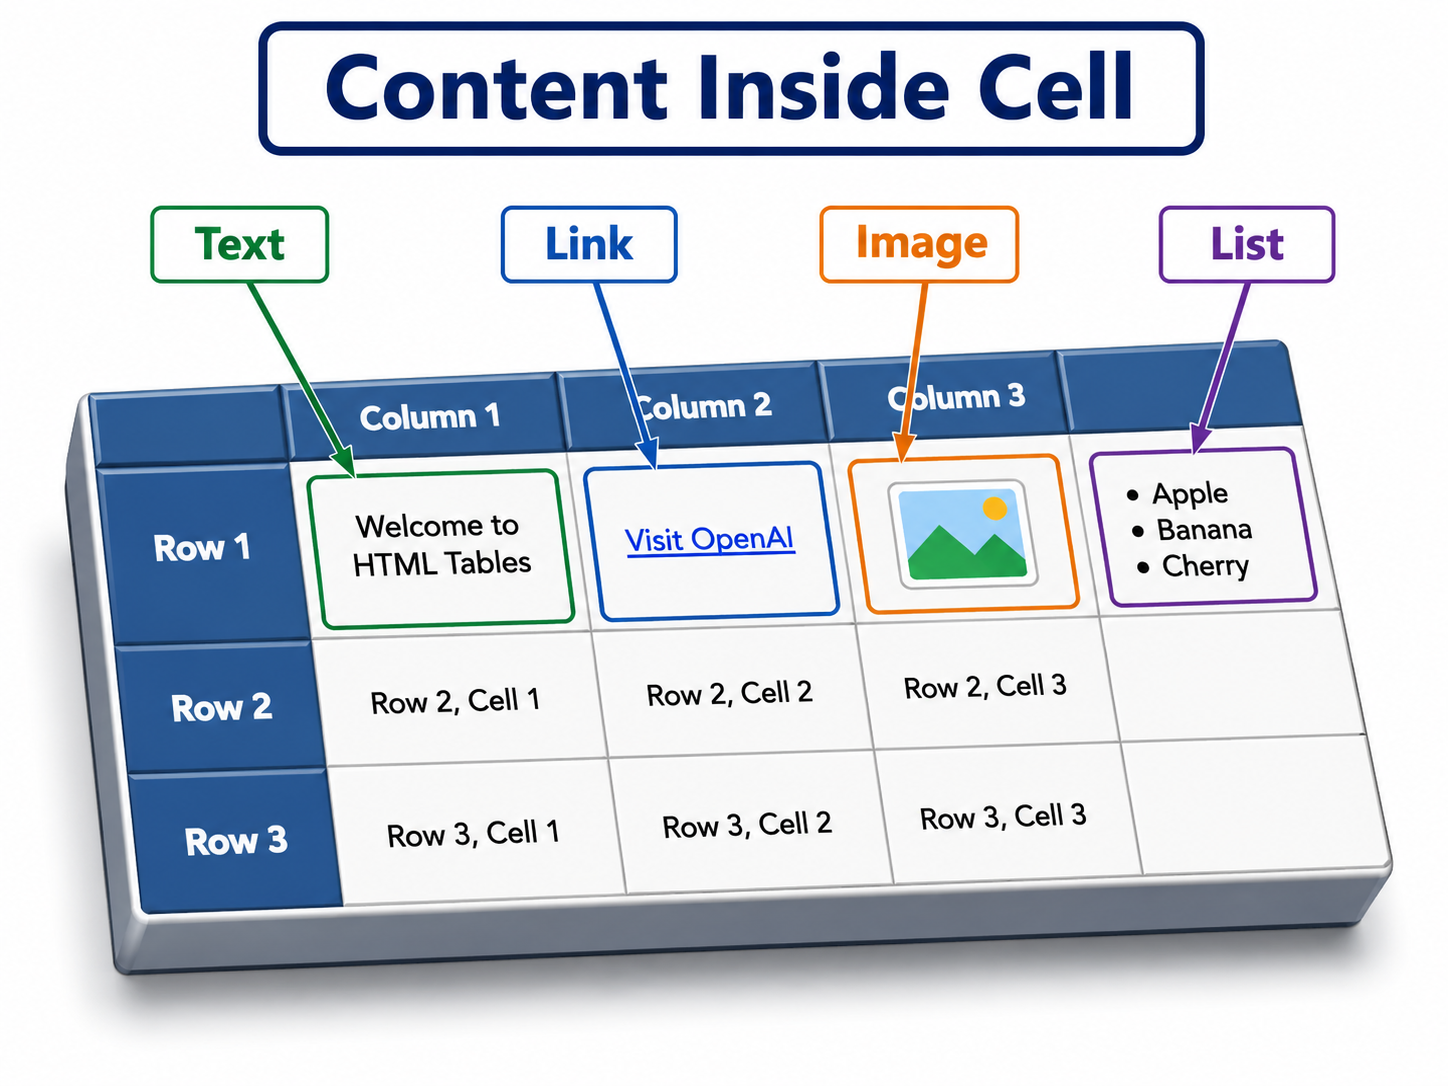
\includegraphics[width=0.78\linewidth,height=0.12\textheight,keepaspectratio]{chapters/Chapter04/topics/images/3d_content_inside_cell.png}
}{
\fbox{\parbox{0.90\linewidth}{\centering\vspace{0.35cm}
\textbf{চিত্র}\\[3pt]
File: \texttt{chapters/Chapter04/topics/images/3d\_content\_inside\_cell.png}
\vspace{0.35cm}}}
}
\captionof{figure}{table cell-এর ভিতরে text, link, image ও list}
\end{center}

\noindent{\color{blue!62!black}\bfseries চিত্র ব্যাখ্যা:}
চিত্রে table cell-এর ভিতরে চার ধরনের content দেখানো হয়েছে: normal text, hyperlink, image এবং ordered list। List cell-এর ভিতরে \texttt{<ol>} ও \texttt{<li>} tag ব্যবহার করা হয়েছে।

\begin{keypointbox}{চিত্র দেখে code লেখার ধাপ}
যে cell-এর ভিতরে list থাকবে, সেখানে প্রথমে \texttt{<td>} লিখবে। তারপর cell-এর ভিতরে \texttt{<ol>} বা \texttt{<ul>} tag লিখে প্রতিটি item \texttt{<li>} দিয়ে লিখবে।
\end{keypointbox}

\begin{examplebox}{কোড}
\begin{verbatim}
<!DOCTYPE html>
<html>
<head>
  <title>List Inside Table Example</title>
</head>
<body>
  <table border="1" cellspacing="0" cellpadding="6">
    <tr>
      <td>
        <ol>
          <li>Dhaka</li>
          <li>Dinajpur</li>
          <li>Rangpur</li>
        </ol>
      </td>
    </tr>
  </table>
</body>
</html>
\end{verbatim}
\end{examplebox}

\subsection{Nested Table বা Table-এর ভিতরে Table}

\begin{definitionbox}{Nested Table}
একটি table-এর কোনো cell-এর ভিতরে আরেকটি table তৈরি করলে তাকে nested table বলা হয়।
\end{definitionbox}

\begin{examplebox}{কোড}
\begin{verbatim}
<!DOCTYPE html>
<html>
<head>
  <title>Nested Table Example</title>
</head>
<body>
  <table border="1" cellspacing="0" cellpadding="10">
    <tr>
      <td>Parent Cell</td>
      <td>
        <table border="1" cellspacing="0" cellpadding="5">
          <tr>
            <th>Child</th>
            <th>Table</th>
          </tr>
          <tr>
            <td>A</td>
            <td>B</td>
          </tr>
        </table>
      </td>
    </tr>
  </table>
</body>
</html>
\end{verbatim}
\end{examplebox}

\conceptwrapimage{chapters/Chapter04/topics/images/3d_nested_table.png}
{চিত্রে parent table-এর একটি cell-এর ভিতরে child table বসানো হয়েছে। এটিকে nested table বা table inside table বলা হয়।}
{table-এর ভিতরে nested table}

\begin{keypointbox}{Nested table লেখার সতর্কতা}
Nested table লিখলে outer table ও inner table-এর tag আলাদা করে close করতে হবে। প্রথমে inner table-এর \texttt{</table>} close করবে, তারপর outer cell-এর \texttt{</td>} এবং শেষে outer table close করবে। ভুল জায়গায় \texttt{</table>} দিলে output ভেঙে যায়।
\end{keypointbox}


\subsection{Modern CSS Note}

\begin{keypointbox}{Modern note}
HSC ICT basic HTML অংশে \texttt{border}, \texttt{align}, \texttt{bgcolor}, \texttt{cellpadding}, \texttt{cellspacing}, \texttt{width} attribute শেখা দরকার। তবে professional web design-এ এগুলোর অনেকগুলো কাজ CSS দিয়ে করা হয়। যেমন: \texttt{border}, \texttt{border-collapse}, \texttt{border-spacing}, \texttt{padding}, \texttt{text-align}, \texttt{background-color}, \texttt{width}।
\end{keypointbox}

\begin{examplebox}{Modern CSS Version}
\begin{verbatim}
<!DOCTYPE html>
<html>
<head>
  <title>Modern Table</title>
  <style>
    table {
      width: 400px;
      border-collapse: collapse;
    }
    th, td {
      border: 1px solid black;
      padding: 8px;
      text-align: center;
    }
    th {
      background-color: lightgray;
    }
  </style>
</head>
<body>
  <table>
    <tr>
      <th>Roll</th>
      <th>Name</th>
    </tr>
    <tr>
      <td>101</td>
      <td>Rafi</td>
    </tr>
  </table>
</body>
</html>
\end{verbatim}
\end{examplebox}

\subsection{Semantic ও Readability Note}

HSC book-style code-এ \texttt{border}, \texttt{cellpadding}, \texttt{cellspacing}, \texttt{align}, \texttt{bgcolor} attribute দেখা যায়। এগুলো practical exam-এর জন্য জানা দরকার। তবে modern HTML-এ table-এর visual style সাধারণত CSS দিয়ে করা হয়। Table-এর meaning পরিষ্কার রাখতে heading cell-এ \texttt{<th>} ব্যবহার করা উচিত এবং table-এর title থাকলে \texttt{<caption>} ব্যবহার করা উচিত।

\begin{boardbox}{ভালো table code-এর বৈশিষ্ট্য}
\begin{itemize}
\item Table data row-column আকারে logical হবে।
\item Heading cell-এ \texttt{<th>} ব্যবহার করা হবে।
\item Caption থাকলে \texttt{<caption>} table-এর শুরুতে লেখা হবে।
\item Image থাকলে \texttt{alt} attribute ব্যবহার করা হবে।
\item Link থাকলে meaningful text ব্যবহার করা হবে।
\item Tag indentation পরিষ্কার হলে code পড়া সহজ হবে।
\end{itemize}
\end{boardbox}

\subsection{চিত্র দেখে Table Code লেখার ধাপ}

HSC exam-এ চিত্র দেখে table code লিখতে হলে আগে table-টি বিশ্লেষণ করতে হবে।

\begin{enumerate}
\item মোট কয়টি row আছে দেখো।
\item সর্বোচ্চ কয়টি column আছে দেখো।
\item heading cell আছে কি না দেখো।
\item কোনো cell merge আছে কি না দেখো।
\item cell merge হলে সেটি \texttt{rowspan} নাকি \texttt{colspan} তা নির্ধারণ করো।
\item border, width, align, cellspacing, cellpadding দরকার কি না দেখো।
\item image, link, list বা nested table আছে কি না দেখো।
\item তারপর \texttt{<table>} skeleton লিখে row অনুযায়ী cell বসাও।
\end{enumerate}

\begin{center}
\IfFileExists{chapters/Chapter04/topics/images/3d_figure_to_code_steps.png}{
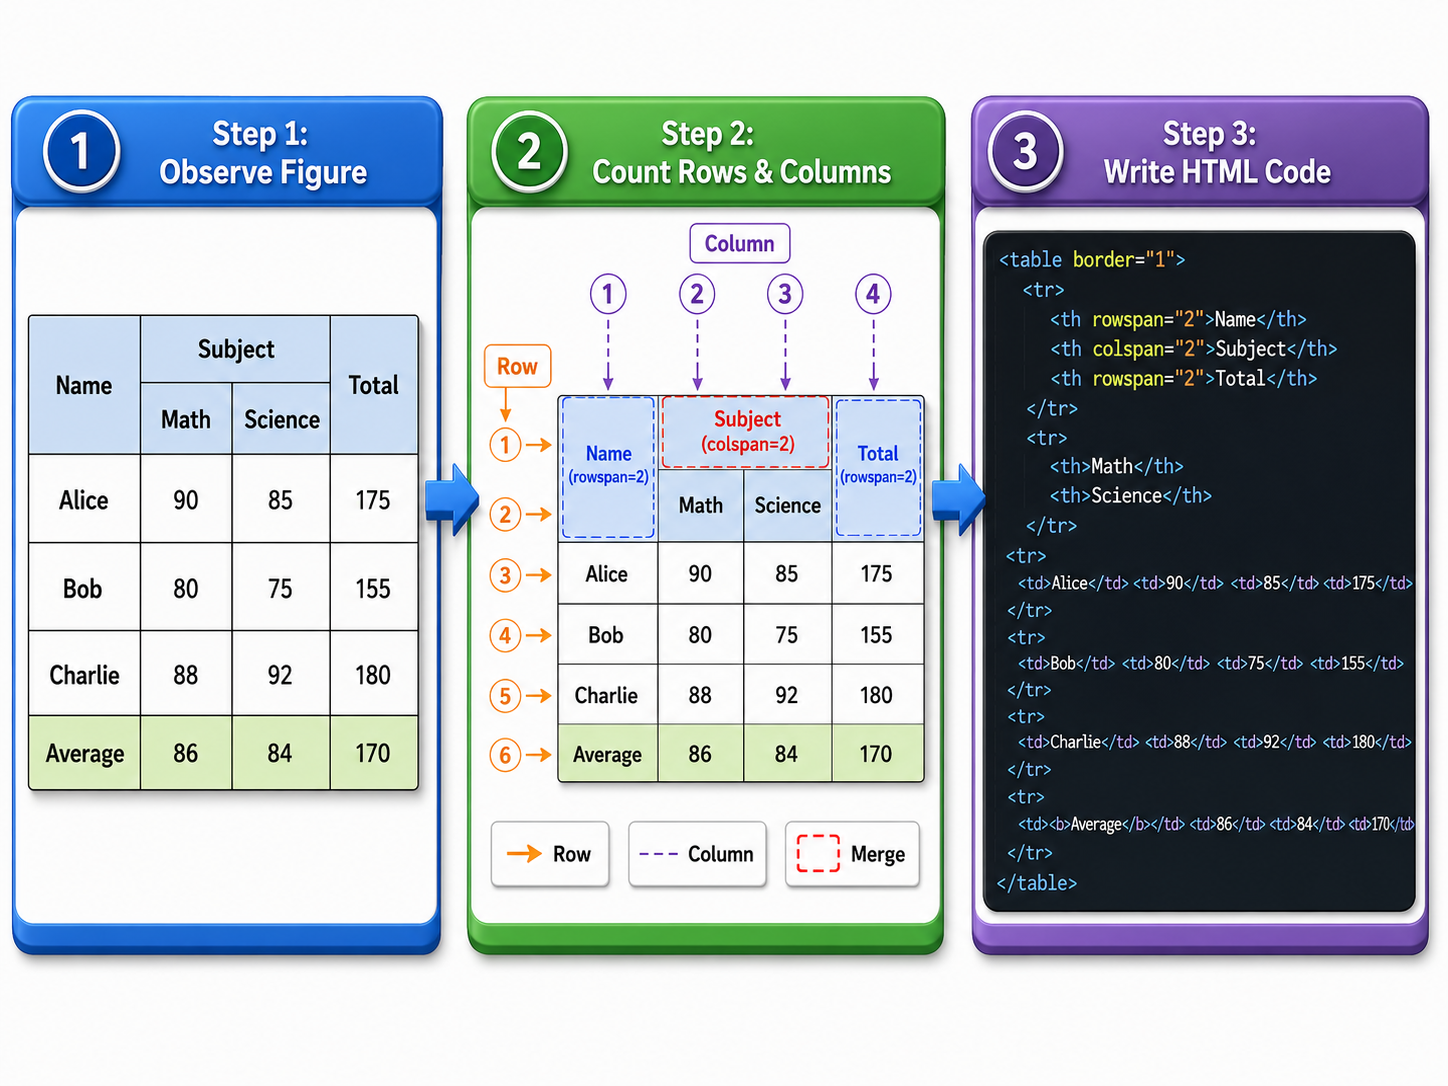
\includegraphics[width=0.95\linewidth,height=0.11\textheight,keepaspectratio]{chapters/Chapter04/topics/images/3d_figure_to_code_steps.png}
}{
\fbox{\parbox{0.90\linewidth}{\centering\vspace{0.5cm}
\textbf{চিত্র}\\[4pt]
A flow diagram: count rows $\rightarrow$ count columns $\rightarrow$ find merged cells $\rightarrow$ add content $\rightarrow$ write HTML code.\\[4pt]
File: \texttt{chapters/Chapter04/topics/images/3d\_figure\_to\_code\_steps.png}
\vspace{0.5cm}}}
}
\captionof{figure}{figure থেকে HTML table code লেখার ধাপ}
\end{center}

\begin{keypointbox}{চিত্র ব্যাখ্যা}
চিত্রে চিত্র দেখে HTML table code লেখার workflow দেখানো হয়েছে: row-column count করা, merged cell identify করা, content type বোঝা এবং শেষে HTML tag লেখা।
\end{keypointbox}


\subsection{PDF Exercise Bank: First to Last}

এই অংশে PDF-এর page অনুযায়ী table exercise সাজানো হয়েছে। প্রত্যেক exercise-এ concept, চিত্র, চিত্র ব্যাখ্যা, code লেখার ধাপ এবং কোড দেওয়া হয়েছে।

\begin{multicols}{2}
\raggedcolumns
\setlength{\columnsep}{10pt}
\subsubsection{Exercise 1: Basic Row and Column Table}

\begin{boardbox}{Concept}
প্রথম table exercise-এ 2 row এবং 2 column দিয়ে basic cell structure বোঝানো হয়েছে।
\end{boardbox}

\begin{center}
\IfFileExists{chapters/Chapter04/topics/images/ex01_3d_basic_2x2.png}{
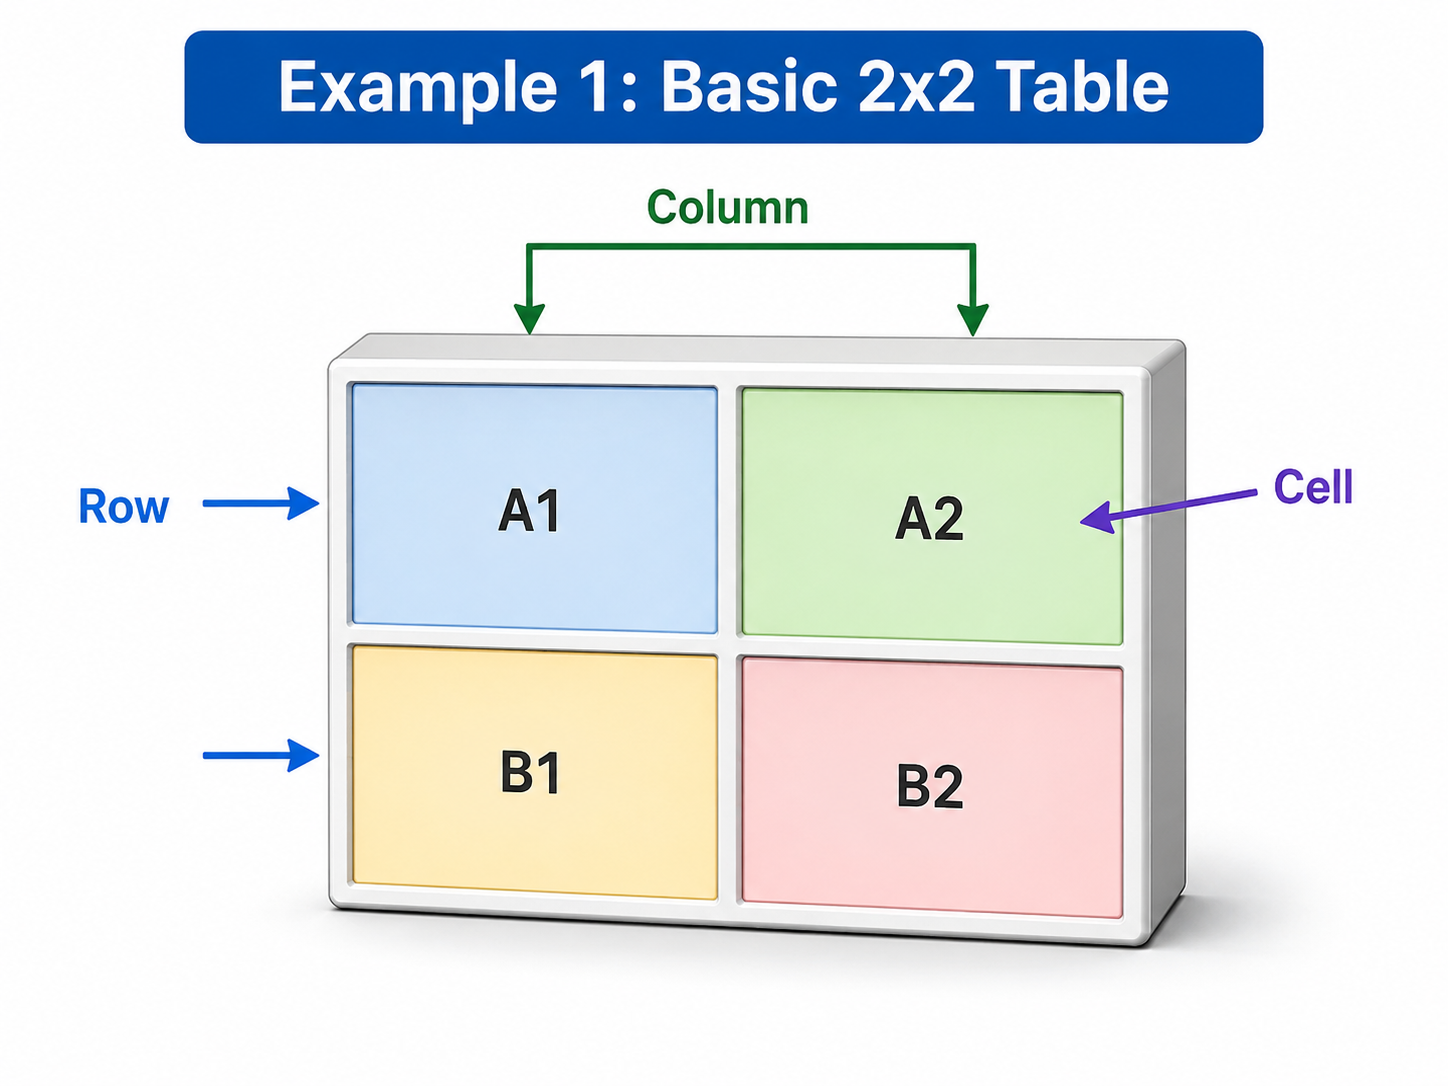
\includegraphics[width=0.95\linewidth,height=0.11\textheight,keepaspectratio]{chapters/Chapter04/topics/images/ex01_3d_basic_2x2.png}
}{
\fbox{\parbox{0.90\linewidth}{\centering\vspace{0.4cm}
\textbf{চিত্র}\\
File: \texttt{chapters/Chapter04/topics/images/ex01\_3d\_basic\_2x2.png}
\vspace{0.4cm}}}
}
\captionof{figure}{Exercise 1-এর table চিত্র}
\end{center}

\begin{keypointbox}{চিত্র ব্যাখ্যা}
চিত্রে A1, A2, B1 এবং B2 নামে চারটি cell আছে। প্রথম row-তে A1-A2 এবং দ্বিতীয় row-তে B1-B2 রাখা হয়েছে।
\end{keypointbox}

\begin{keypointbox}{চিত্র দেখে code লেখার ধাপ}
প্রথমে 2টি row ধরবে। প্রতিটি row-তে 2টি করে \texttt{<td>} cell লিখবে। তারপর cell text হিসেবে A1, A2, B1, B2 বসাবে।
\end{keypointbox}

\par\noindent{\color{purple!70!black}\bfseries\small কোড}\par\vspace{-4pt}
\begin{verbatim}
<!DOCTYPE html>
<html>
<head>
  <title>HTML Table Example</title>
</head>
<body>
<table>
  <tr>
    <td>A1</td>
    <td>A2</td>
  </tr>
  <tr>
    <td>B1</td>
    <td>B2</td>
  </tr>
</table>
</body>
</html>
\end{verbatim}
\vspace{-6pt}

\subsubsection{Exercise 2: Border সহ Simple Table}

\begin{boardbox}{Concept}
\texttt{border="1"} দিলে table এবং cell-এর চারপাশে border দেখা যায়।
\end{boardbox}

\begin{center}
\IfFileExists{chapters/Chapter04/topics/images/ex02_3d_border_table.png}{
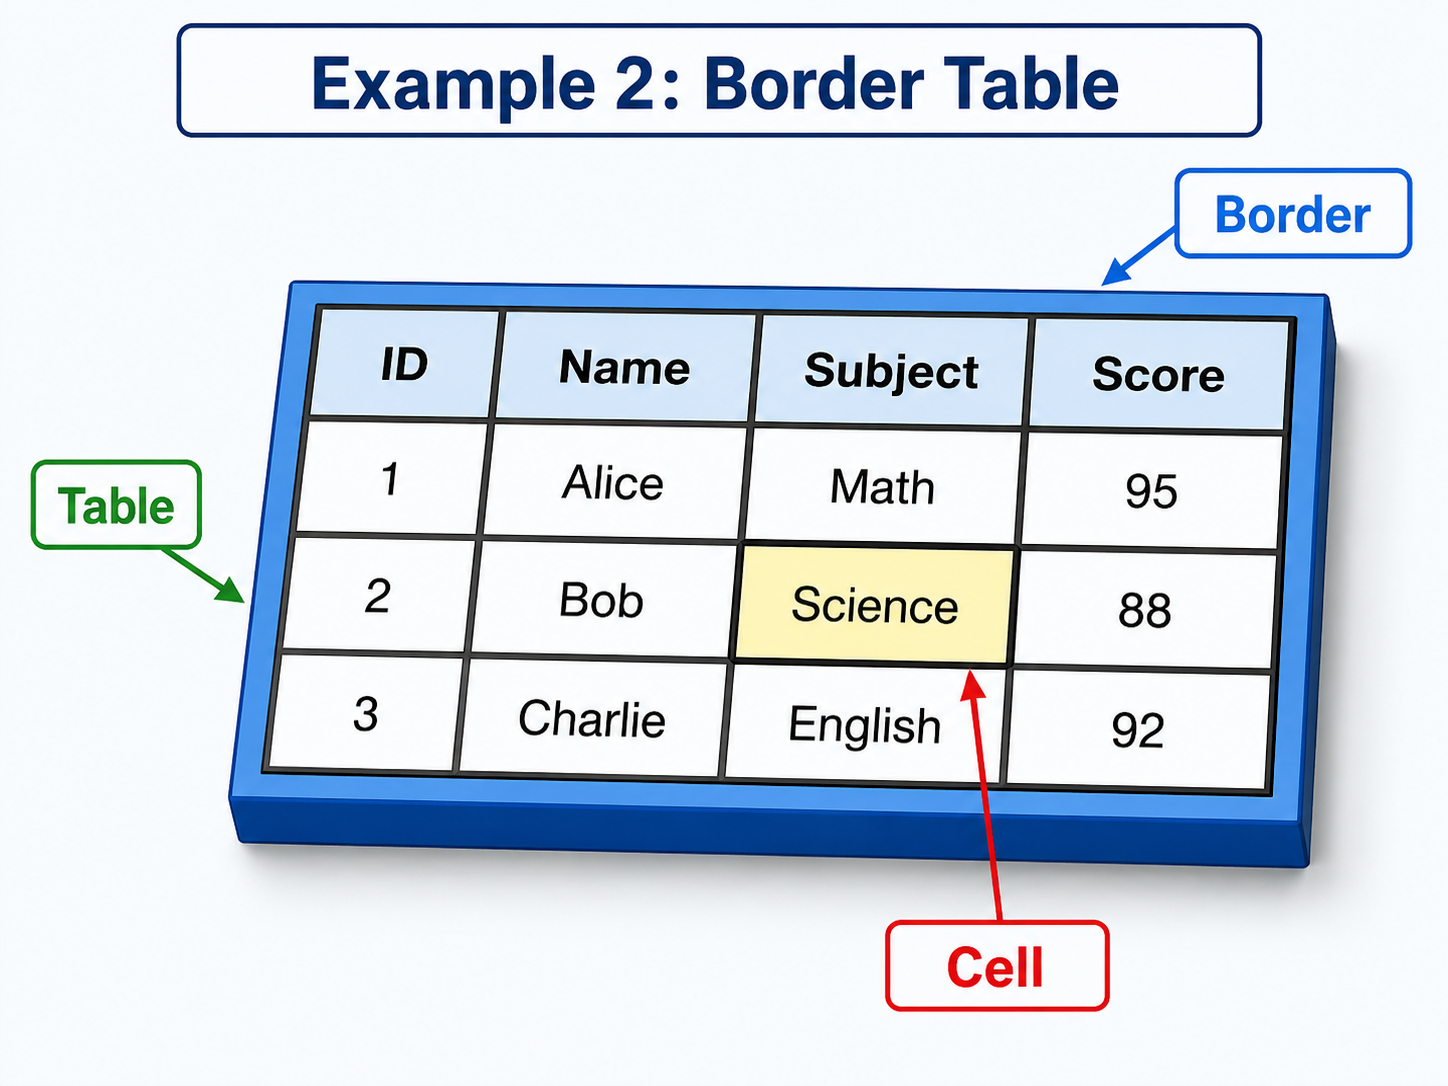
\includegraphics[width=0.95\linewidth,height=0.11\textheight,keepaspectratio]{chapters/Chapter04/topics/images/ex02_3d_border_table.png}
}{
\fbox{\parbox{0.90\linewidth}{\centering\vspace{0.4cm}
\textbf{চিত্র}\\
File: \texttt{chapters/Chapter04/topics/images/ex02\_3d\_border\_table.png}
\vspace{0.4cm}}}
}
\captionof{figure}{Exercise 2-এর border চিত্র}
\end{center}

\begin{keypointbox}{চিত্র ব্যাখ্যা}
চিত্রে ID, Name, Subject এবং Score column আছে। তিনজন student-এর subject ও score border সহ table আকারে দেখানো হয়েছে।
\end{keypointbox}

\begin{keypointbox}{চিত্র দেখে code লেখার ধাপ}
প্রথমে header row-তে চারটি \texttt{<th>} লিখবে। এরপর Alice, Bob ও Charlie-এর জন্য তিনটি data row তৈরি করবে। পুরো table-এ border দেখাতে \texttt{border="1"} ব্যবহার করবে।
\end{keypointbox}

\par\noindent{\color{purple!70!black}\bfseries\small কোড}\par\vspace{-4pt}
\begin{verbatim}
<!DOCTYPE html>
<html>
<head>
  <title>HTML Table Example</title>
</head>
<body>
<table border="1" cellspacing="0" cellpadding="6">
  <tr>
    <th>ID</th>
    <th>Name</th>
    <th>Subject</th>
    <th>Score</th>
  </tr>
  <tr>
    <td>1</td>
    <td>Alice</td>
    <td>Math</td>
    <td>95</td>
  </tr>
  <tr>
    <td>2</td>
    <td>Bob</td>
    <td>Science</td>
    <td>88</td>
  </tr>
  <tr>
    <td>3</td>
    <td>Charlie</td>
    <td>English</td>
    <td>92</td>
  </tr>
</table>
</body>
</html>
\end{verbatim}
\vspace{-6pt}

\subsubsection{Exercise 3: Caption, TH এবং Student Info Table}

\begin{boardbox}{Concept}
\texttt{<caption>} table-এর title দেয় এবং \texttt{<th>} heading cell তৈরি করে।
\end{boardbox}

\begin{center}
\IfFileExists{chapters/Chapter04/topics/images/ex03_3d_student_info.png}{
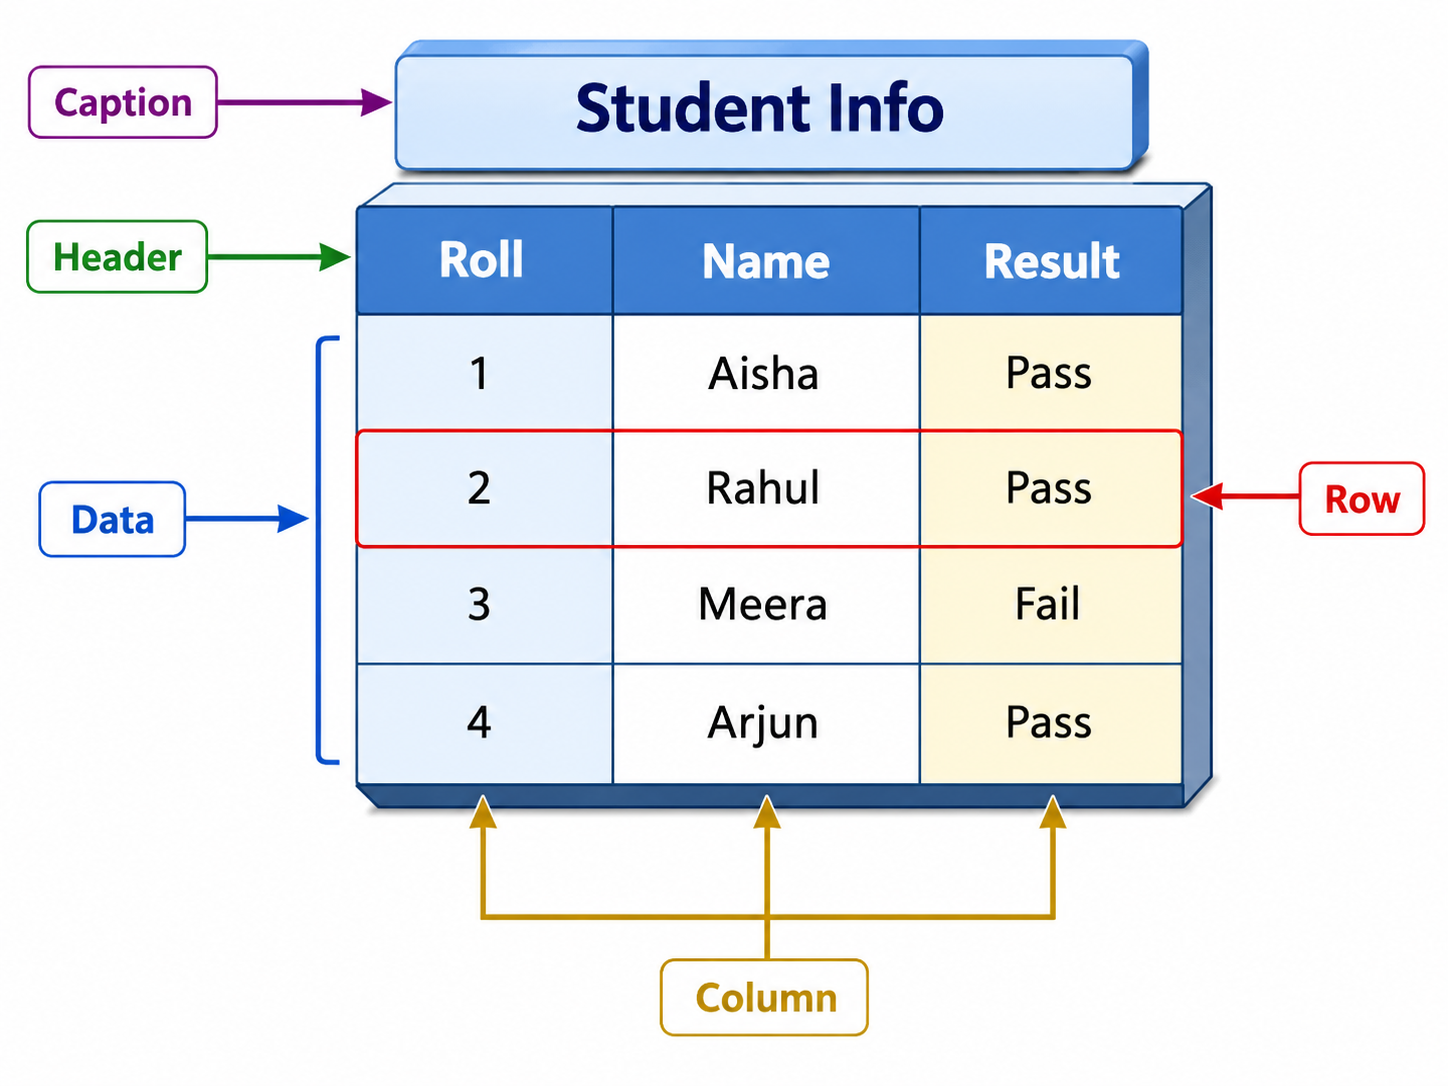
\includegraphics[width=0.95\linewidth,height=0.11\textheight,keepaspectratio]{chapters/Chapter04/topics/images/ex03_3d_student_info.png}
}{
\fbox{\parbox{0.90\linewidth}{\centering\vspace{0.4cm}
\textbf{চিত্র}\\
File: \texttt{chapters/Chapter04/topics/images/ex03\_3d\_student\_info.png}
\vspace{0.4cm}}}
}
\captionof{figure}{Exercise 3-এর caption ও heading চিত্র}
\end{center}

\begin{keypointbox}{চিত্র ব্যাখ্যা}
চিত্রে Student Info caption আছে। table-এ Roll, Name ও Result column দেখানো হয়েছে এবং data row-গুলোতে Pass/Fail result আছে।
\end{keypointbox}

\begin{keypointbox}{চিত্র দেখে code লেখার ধাপ}
প্রথমে \texttt{<caption>} দিয়ে Student Info লিখবে। এরপর তিনটি header cell তৈরি করবে। তারপর চারটি student row লিখবে।
\end{keypointbox}

\par\noindent{\color{purple!70!black}\bfseries\small কোড}\par\vspace{-4pt}
\begin{verbatim}
<!DOCTYPE html>
<html>
<head>
  <title>HTML Table Example</title>
</head>
<body>
<table border="1" cellspacing="0" cellpadding="6">
  <caption><b>Student Info</b></caption>
  <tr>
    <th>Roll</th>
    <th>Name</th>
    <th>Result</th>
  </tr>
  <tr><td>1</td><td>Aisha</td><td>Pass</td></tr>
  <tr><td>2</td><td>Rahul</td><td>Pass</td></tr>
  <tr><td>3</td><td>Meera</td><td>Fail</td></tr>
  <tr><td>4</td><td>Arjun</td><td>Pass</td></tr>
</table>
</body>
</html>
\end{verbatim}
\vspace{-6pt}

\subsubsection{Exercise 4: Width Attribute দিয়ে Table Width নির্ধারণ}

\begin{boardbox}{Concept}
\texttt{width} attribute দিয়ে table-এর মোট প্রস্থ নির্ধারণ করা যায়।
\end{boardbox}

\begin{center}
\IfFileExists{chapters/Chapter04/topics/images/ex04_3d_width_400.png}{
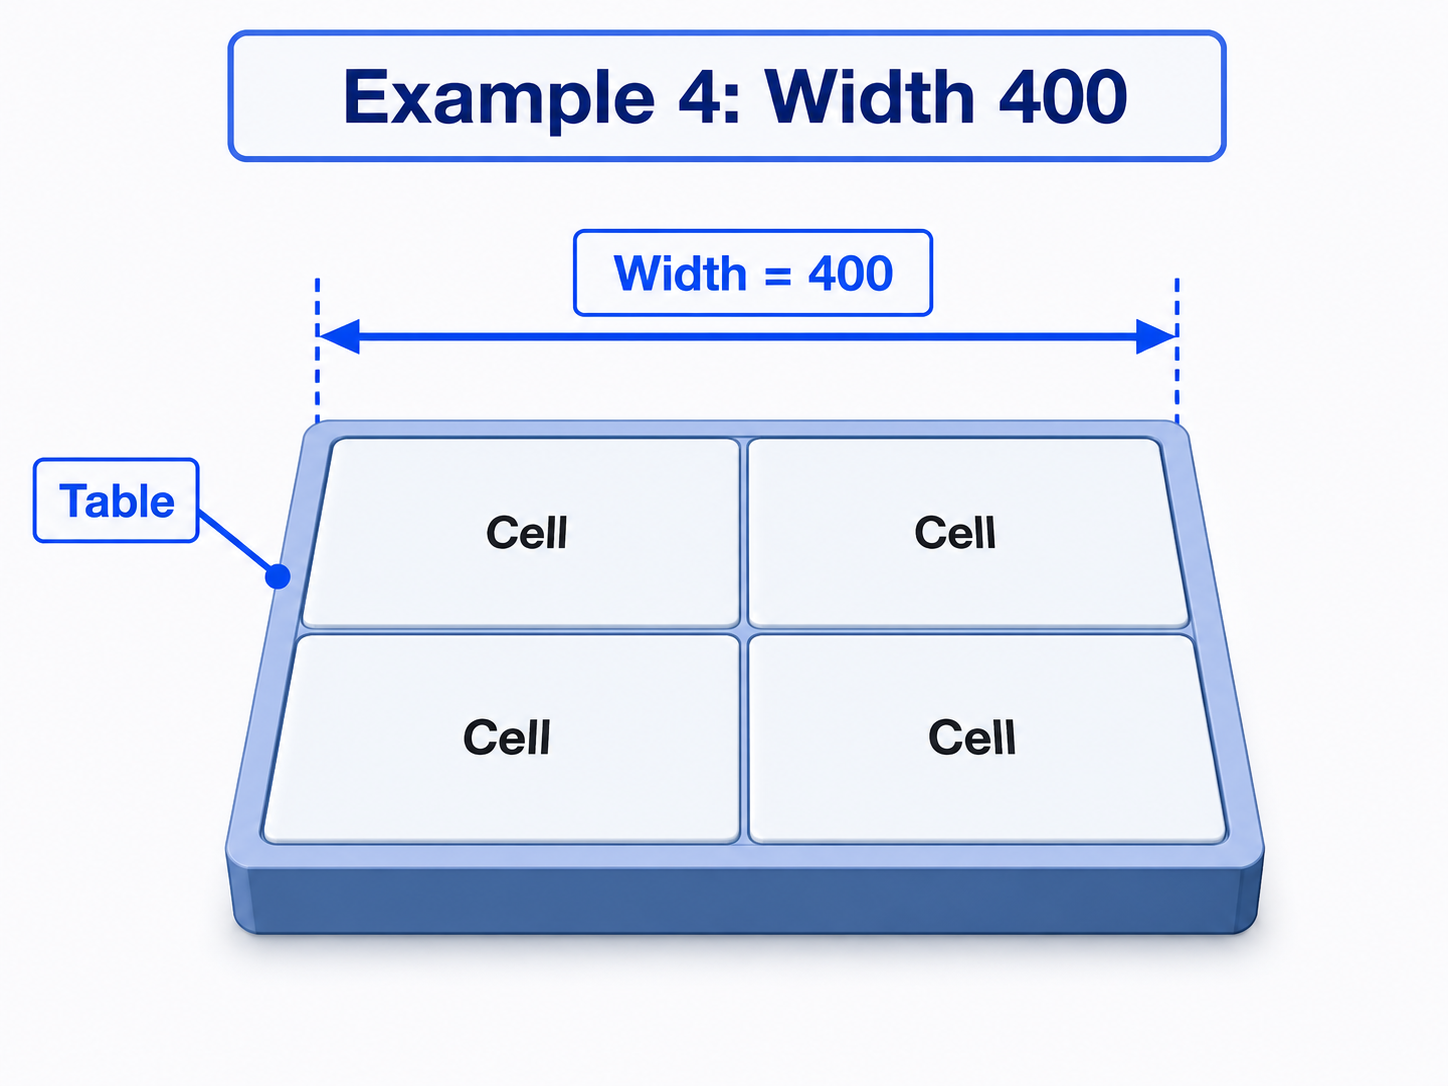
\includegraphics[width=0.95\linewidth,height=0.11\textheight,keepaspectratio]{chapters/Chapter04/topics/images/ex04_3d_width_400.png}
}{
\fbox{\parbox{0.90\linewidth}{\centering\vspace{0.4cm}
\textbf{চিত্র}\\
File: \texttt{chapters/Chapter04/topics/images/ex04\_3d\_width\_400.png}
\vspace{0.4cm}}}
}
\captionof{figure}{Exercise 4-এর width চিত্র}
\end{center}

\begin{keypointbox}{চিত্র ব্যাখ্যা}
চিত্রে table width 400 দেখানো হয়েছে। table-টি 2 row ও 2 column-এর, প্রতিটি cell-এ Cell লেখা আছে।
\end{keypointbox}

\begin{keypointbox}{চিত্র দেখে code লেখার ধাপ}
প্রথমে \texttt{width="400"} সহ table লিখবে। তারপর 2টি row এবং প্রতিটি row-তে 2টি cell তৈরি করবে।
\end{keypointbox}

\par\noindent{\color{purple!70!black}\bfseries\small কোড}\par\vspace{-4pt}
\begin{verbatim}
<!DOCTYPE html>
<html>
<head>
  <title>HTML Table Example</title>
</head>
<body>
<table border="1" width="400" cellspacing="0" cellpadding="10">
  <tr>
    <td>Cell</td>
    <td>Cell</td>
  </tr>
  <tr>
    <td>Cell</td>
    <td>Cell</td>
  </tr>
</table>
</body>
</html>
\end{verbatim}
\vspace{-6pt}

\subsubsection{Exercise 5: Table Attribute Practice}

\begin{boardbox}{Concept}
একই table-এ \texttt{border}, \texttt{width}, \texttt{cellspacing}, \texttt{cellpadding}, \texttt{align} ও \texttt{bgcolor} attribute ব্যবহার করা যায়।
\end{boardbox}

\begin{center}
\IfFileExists{chapters/Chapter04/topics/images/ex05_3d_table_attributes_combined.png}{
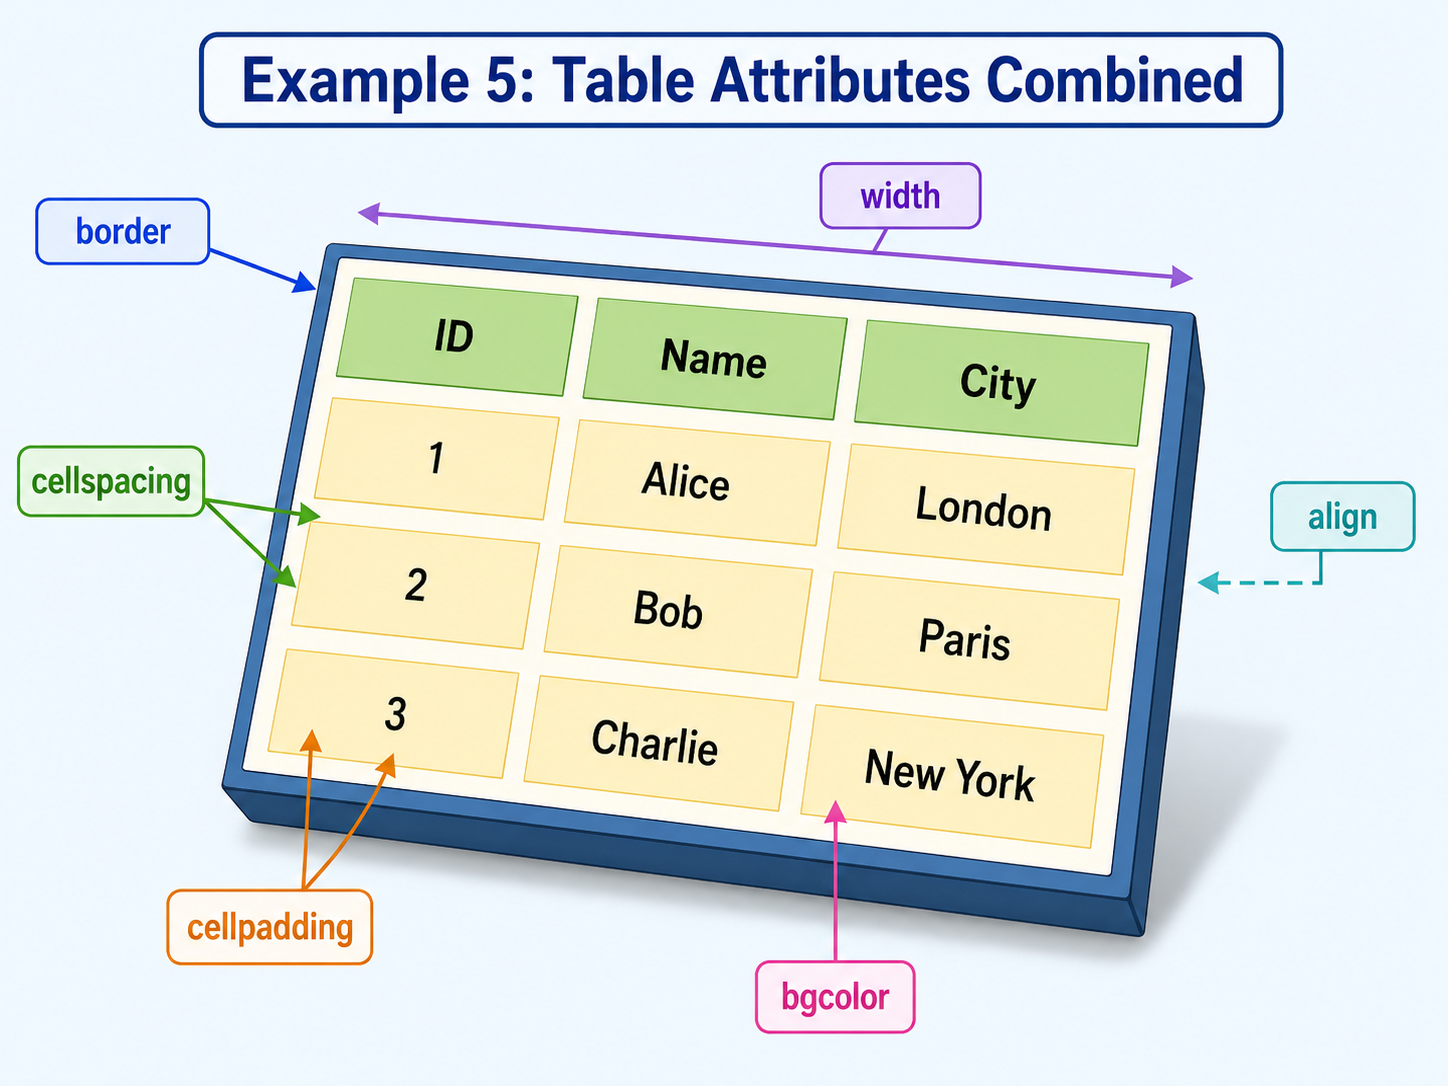
\includegraphics[width=0.95\linewidth,height=0.11\textheight,keepaspectratio]{chapters/Chapter04/topics/images/ex05_3d_table_attributes_combined.png}
}{
\fbox{\parbox{0.90\linewidth}{\centering\vspace{0.4cm}
\textbf{চিত্র}\\
File: \texttt{chapters/Chapter04/topics/images/ex05\_3d\_table\_attributes\_combined.png}
\vspace{0.4cm}}}
}
\captionof{figure}{Exercise 5-এর attribute চিত্র}
\end{center}

\begin{keypointbox}{চিত্র ব্যাখ্যা}
চিত্রে একটি student/city table-এর উপর table attributes-এর effect দেখানো হয়েছে। header background color, table width, border, spacing, padding এবং alignment visual label দিয়ে বোঝানো হয়েছে।
\end{keypointbox}

\begin{keypointbox}{চিত্র দেখে code লেখার ধাপ}
প্রথমে table tag-এ attribute বসাবে। তারপর ID, Name, City header row লিখবে। শেষে তিনটি data row তৈরি করবে।
\end{keypointbox}

\par\noindent{\color{purple!70!black}\bfseries\small কোড}\par\vspace{-4pt}
\begin{verbatim}
<!DOCTYPE html>
<html>
<head>
  <title>HTML Table Example</title>
</head>
<body>
<table border="1" width="450" cellspacing="6" cellpadding="8" align="center">
  <tr bgcolor="lightgreen">
    <th>ID</th>
    <th>Name</th>
    <th>City</th>
  </tr>
  <tr><td>1</td><td>Alice</td><td>London</td></tr>
  <tr><td>2</td><td>Bob</td><td>Paris</td></tr>
  <tr><td>3</td><td>Charlie</td><td>New York</td></tr>
</table>
</body>
</html>
\end{verbatim}
\vspace{-6pt}

\subsubsection{Exercise 6: Colspan ও Rowspan Basic Example}

\begin{boardbox}{Concept}
\texttt{colspan} horizontal cell merge করে এবং \texttt{rowspan} vertical cell merge করে।
\end{boardbox}

\begin{center}
\IfFileExists{chapters/Chapter04/topics/images/ex06_3d_span_two_columns_rows.png}{
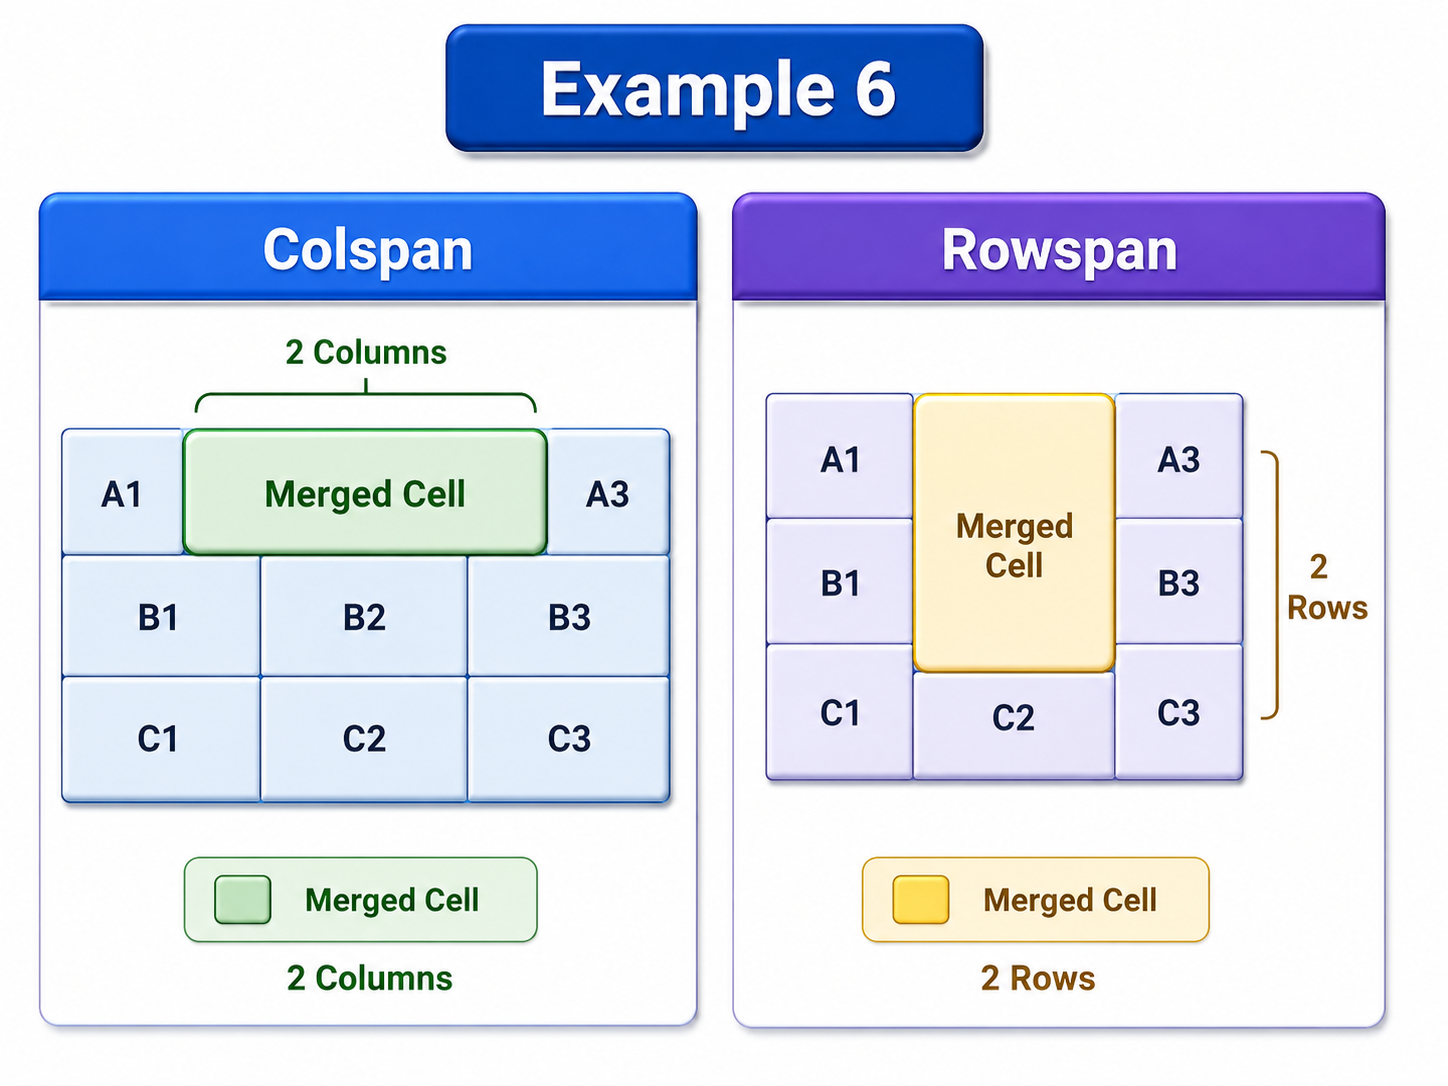
\includegraphics[width=0.95\linewidth,height=0.11\textheight,keepaspectratio]{chapters/Chapter04/topics/images/ex06_3d_span_two_columns_rows.png}
}{
\fbox{\parbox{0.90\linewidth}{\centering\vspace{0.4cm}
\textbf{চিত্র}\\
File: \texttt{chapters/Chapter04/topics/images/ex06\_3d\_span\_two\_columns\_rows.png}
\vspace{0.4cm}}}
}
\captionof{figure}{Exercise 6-এর rowspan-colspan চিত্র}
\end{center}

\begin{keypointbox}{চিত্র ব্যাখ্যা}
চিত্রে বাম পাশে colspan দিয়ে দুই column merge এবং ডান পাশে rowspan দিয়ে দুই row merge দেখানো হয়েছে।
\end{keypointbox}

\begin{keypointbox}{চিত্র দেখে code লেখার ধাপ}
Horizontal merge দরকার হলে \texttt{colspan="2"} ব্যবহার করবে। Vertical merge দরকার হলে \texttt{rowspan="2"} ব্যবহার করবে।
\end{keypointbox}

\par\noindent{\color{purple!70!black}\bfseries\small কোড}\par\vspace{-4pt}
\begin{verbatim}
<!DOCTYPE html>
<html>
<head>
  <title>HTML Table Example</title>
</head>
<body>
<h3>Colspan</h3>
<table border="1" cellspacing="0" cellpadding="6">
  <tr><th colspan="3">Colspan</th></tr>
  <tr><td>A1</td><td colspan="2">Merged Cell</td></tr>
  <tr><td>B1</td><td>B2</td><td>B3</td></tr>
  <tr><td>C1</td><td>C2</td><td>C3</td></tr>
</table>

<h3>Rowspan</h3>
<table border="1" cellspacing="0" cellpadding="6">
  <tr><th colspan="3">Rowspan</th></tr>
  <tr><td>A1</td><td rowspan="2">Merged Cell</td><td>A3</td></tr>
  <tr><td>B1</td><td>B3</td></tr>
  <tr><td>C1</td><td>C2</td><td>C3</td></tr>
</table>
</body>
</html>
\end{verbatim}
\vspace{-6pt}

\subsubsection{Exercise 7: Empty Cell এবং Basic Sales Table}

\begin{boardbox}{Concept}
খালি cell দেখাতে cell-এর ভিতরে \texttt{\&nbsp;} ব্যবহার করা যায়।
\end{boardbox}

\begin{center}
\IfFileExists{chapters/Chapter04/topics/images/ex07_3d_empty_cells.png}{
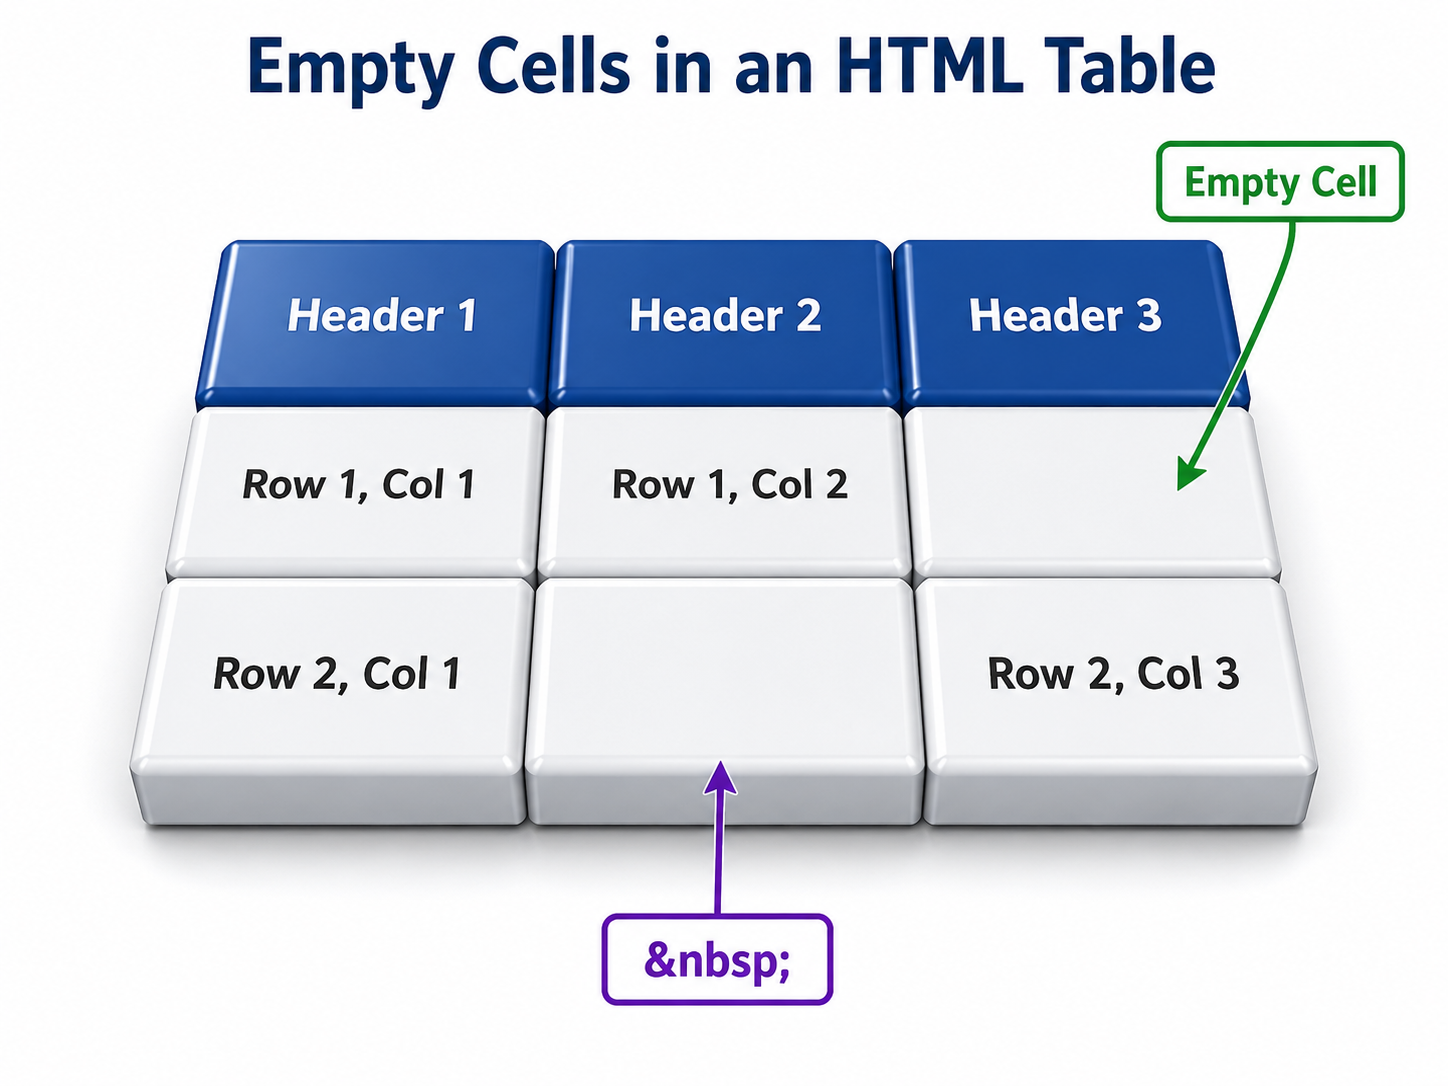
\includegraphics[width=0.95\linewidth,height=0.11\textheight,keepaspectratio]{chapters/Chapter04/topics/images/ex07_3d_empty_cells.png}
}{
\fbox{\parbox{0.90\linewidth}{\centering\vspace{0.4cm}
\textbf{চিত্র}\\
File: \texttt{chapters/Chapter04/topics/images/ex07\_3d\_empty\_cells.png}
\vspace{0.4cm}}}
}
\captionof{figure}{Exercise 7-এর empty cell চিত্র}
\end{center}

\begin{keypointbox}{চিত্র ব্যাখ্যা}
চিত্রে Header 1, Header 2, Header 3 সহ table আছে। কিছু cell intentionally empty রাখা হয়েছে; browser-এ cell visible রাখতে \texttt{\&nbsp;} ব্যবহার করা হয়েছে।
\end{keypointbox}

\begin{keypointbox}{চিত্র দেখে code লেখার ধাপ}
প্রথমে তিনটি header লিখবে। যে cell খালি দেখাতে হবে সেখানে normal text না দিয়ে \texttt{\&nbsp;} লিখবে।
\end{keypointbox}

\par\noindent{\color{purple!70!black}\bfseries\small কোড}\par\vspace{-4pt}
\begin{verbatim}
<!DOCTYPE html>
<html>
<head>
  <title>HTML Table Example</title>
</head>
<body>
<table border="1" cellspacing="0" cellpadding="8">
  <tr>
    <th>Header 1</th>
    <th>Header 2</th>
    <th>Header 3</th>
  </tr>
  <tr>
    <td>Row 1, Col 1</td>
    <td>Row 1, Col 2</td>
    <td>&nbsp;</td>
  </tr>
  <tr>
    <td>Row 2, Col 1</td>
    <td>&nbsp;</td>
    <td>Row 2, Col 3</td>
  </tr>
</table>
</body>
</html>
\end{verbatim}
\vspace{-6pt}

\subsubsection{Exercise 8: Align Attribute Practice}

\begin{boardbox}{Concept}
\texttt{align="center"} দিলে cell-এর content horizontally center হয়।
\end{boardbox}

\begin{center}
\IfFileExists{chapters/Chapter04/topics/images/ex08_3d_align_center.png}{
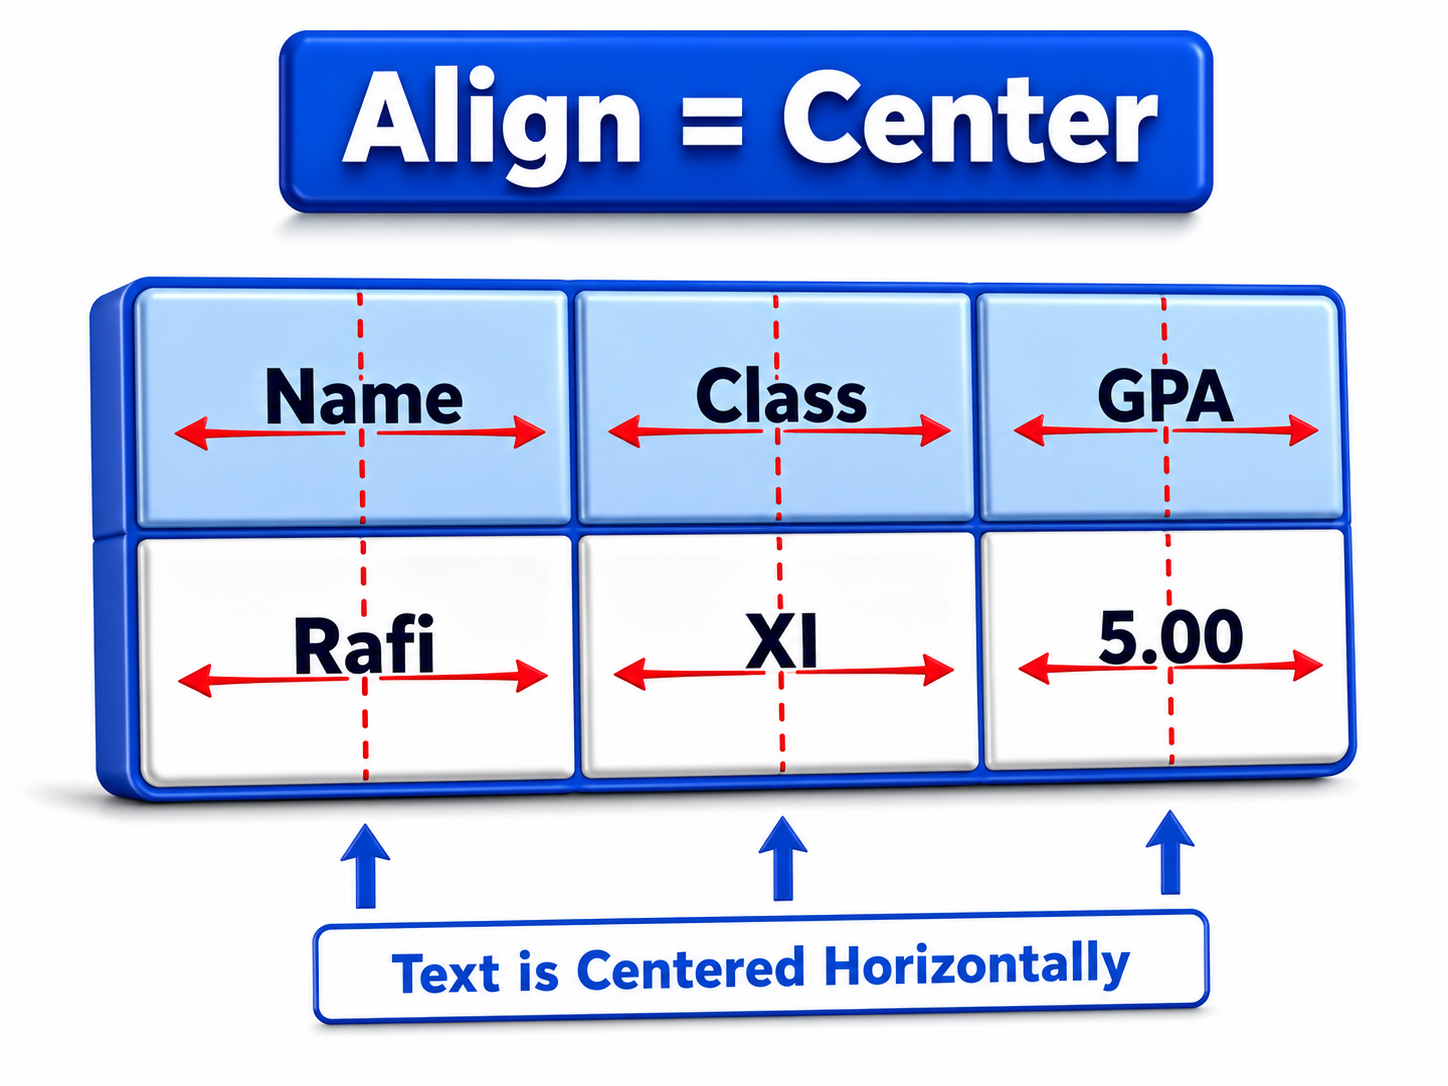
\includegraphics[width=0.95\linewidth,height=0.11\textheight,keepaspectratio]{chapters/Chapter04/topics/images/ex08_3d_align_center.png}
}{
\fbox{\parbox{0.90\linewidth}{\centering\vspace{0.4cm}
\textbf{চিত্র}\\
File: \texttt{chapters/Chapter04/topics/images/ex08\_3d\_align\_center.png}
\vspace{0.4cm}}}
}
\captionof{figure}{Exercise 8-এর align চিত্র}
\end{center}

\begin{keypointbox}{চিত্র ব্যাখ্যা}
চিত্রে Name, Class ও GPA column-এর text center aligned আছে। Rafi, XI এবং 5.00 cell-গুলো cell-এর মাঝখানে বসেছে।
\end{keypointbox}

\begin{keypointbox}{চিত্র দেখে code লেখার ধাপ}
পুরো table center alignment করতে table row বা প্রতিটি cell-এ \texttt{align="center"} ব্যবহার করবে।
\end{keypointbox}

\par\noindent{\color{purple!70!black}\bfseries\small কোড}\par\vspace{-4pt}
\begin{verbatim}
<!DOCTYPE html>
<html>
<head>
  <title>HTML Table Example</title>
</head>
<body>
<table border="1" cellspacing="0" cellpadding="8" align="center">
  <tr align="center">
    <th>Name</th>
    <th>Class</th>
    <th>GPA</th>
  </tr>
  <tr align="center">
    <td>Rafi</td>
    <td>XI</td>
    <td>5.00</td>
  </tr>
</table>
</body>
</html>
\end{verbatim}
\vspace{-6pt}

\subsubsection{Exercise 9: Cell Data Alignment Table}

\begin{boardbox}{Concept}
একই table-এ left, center এবং right alignment আলাদা cell-এ ব্যবহার করা যায়।
\end{boardbox}

\begin{center}
\IfFileExists{chapters/Chapter04/topics/images/ex09_3d_cell_alignment.png}{
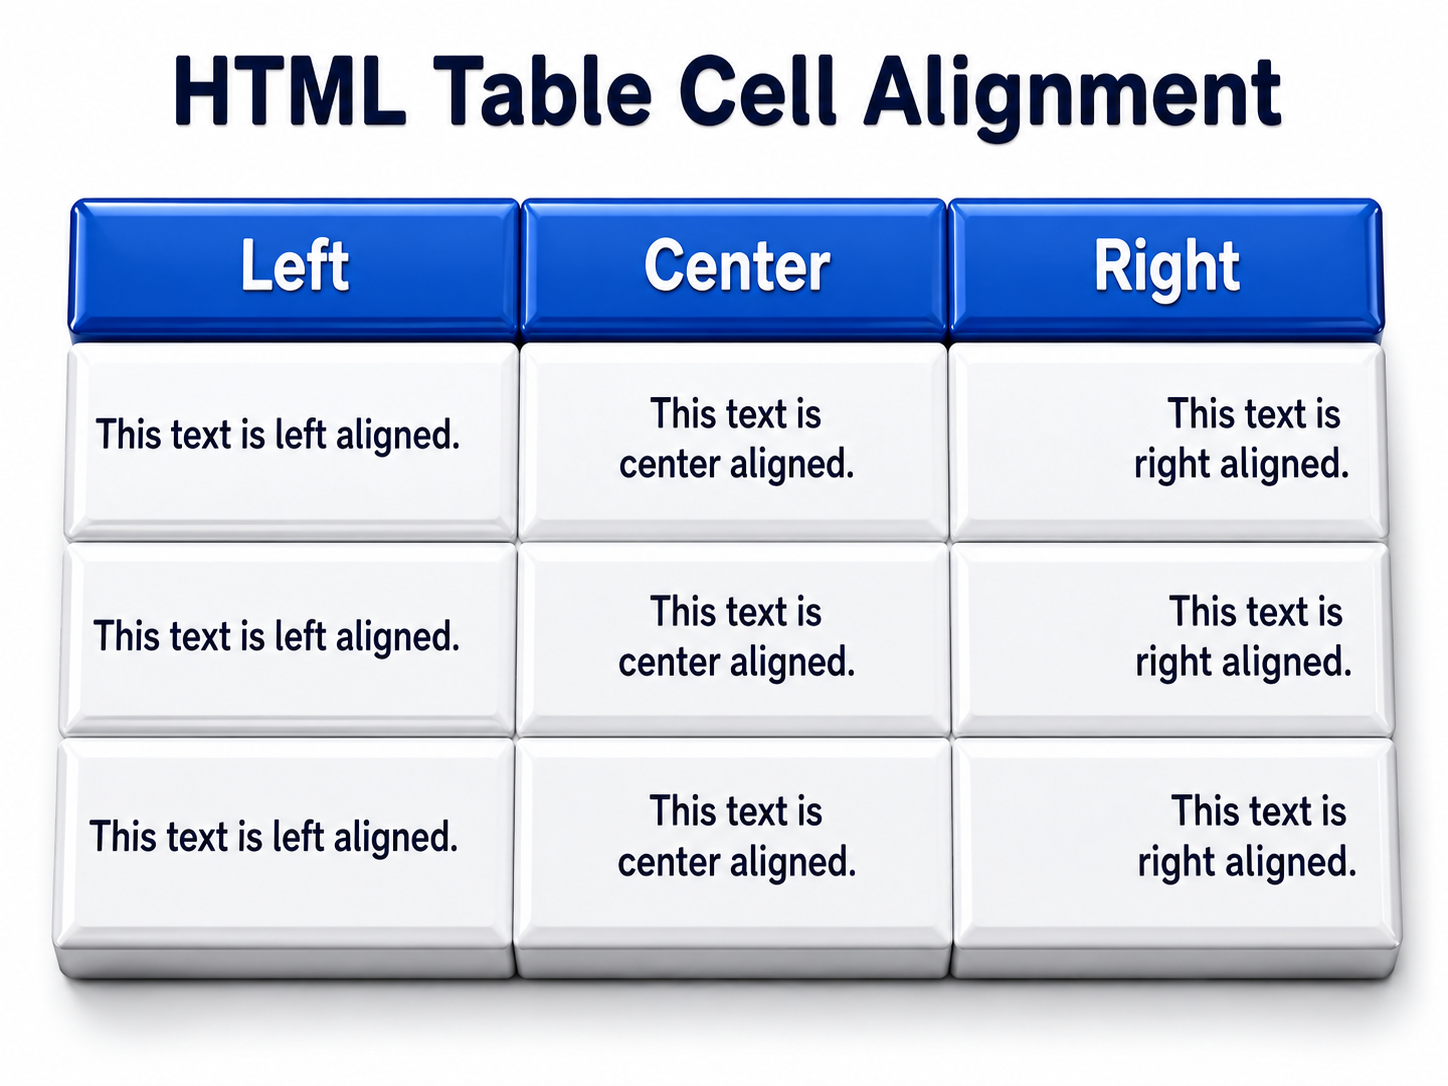
\includegraphics[width=0.95\linewidth,height=0.11\textheight,keepaspectratio]{chapters/Chapter04/topics/images/ex09_3d_cell_alignment.png}
}{
\fbox{\parbox{0.90\linewidth}{\centering\vspace{0.4cm}
\textbf{চিত্র}\\
File: \texttt{chapters/Chapter04/topics/images/ex09\_3d\_cell\_alignment.png}
\vspace{0.4cm}}}
}
\captionof{figure}{Exercise 9-এর cell alignment চিত্র}
\end{center}

\begin{keypointbox}{চিত্র ব্যাখ্যা}
চিত্রে তিনটি column আছে: Left, Center, Right। প্রতিটি column-এর text নিজ নিজ alignment অনুযায়ী cell-এর বাম, মাঝ বা ডান পাশে বসেছে।
\end{keypointbox}

\begin{keypointbox}{চিত্র দেখে code লেখার ধাপ}
Left column-এর cell-এ \texttt{align="left"}, center column-এ \texttt{align="center"} এবং right column-এ \texttt{align="right"} ব্যবহার করবে।
\end{keypointbox}

\par\noindent{\color{purple!70!black}\bfseries\small কোড}\par\vspace{-4pt}
\begin{verbatim}
<!DOCTYPE html>
<html>
<head>
  <title>HTML Table Example</title>
</head>
<body>
<table border="1" cellspacing="0" cellpadding="8">
  <tr>
    <th>Left</th>
    <th>Center</th>
    <th>Right</th>
  </tr>
  <tr>
    <td align="left">This text is left aligned.</td>
    <td align="center">This text is center aligned.</td>
    <td align="right">This text is right aligned.</td>
  </tr>
  <tr>
    <td align="left">This text is left aligned.</td>
    <td align="center">This text is center aligned.</td>
    <td align="right">This text is right aligned.</td>
  </tr>
</table>
</body>
</html>
\end{verbatim}
\vspace{-6pt}

\subsubsection{Exercise 10: Cell Width/Height Change}

\begin{boardbox}{Concept}
\texttt{width} ও \texttt{height} attribute দিয়ে cell-এর size change করা যায়।
\end{boardbox}

\begin{center}
\IfFileExists{chapters/Chapter04/topics/images/ex10_3d_cell_width_height.png}{
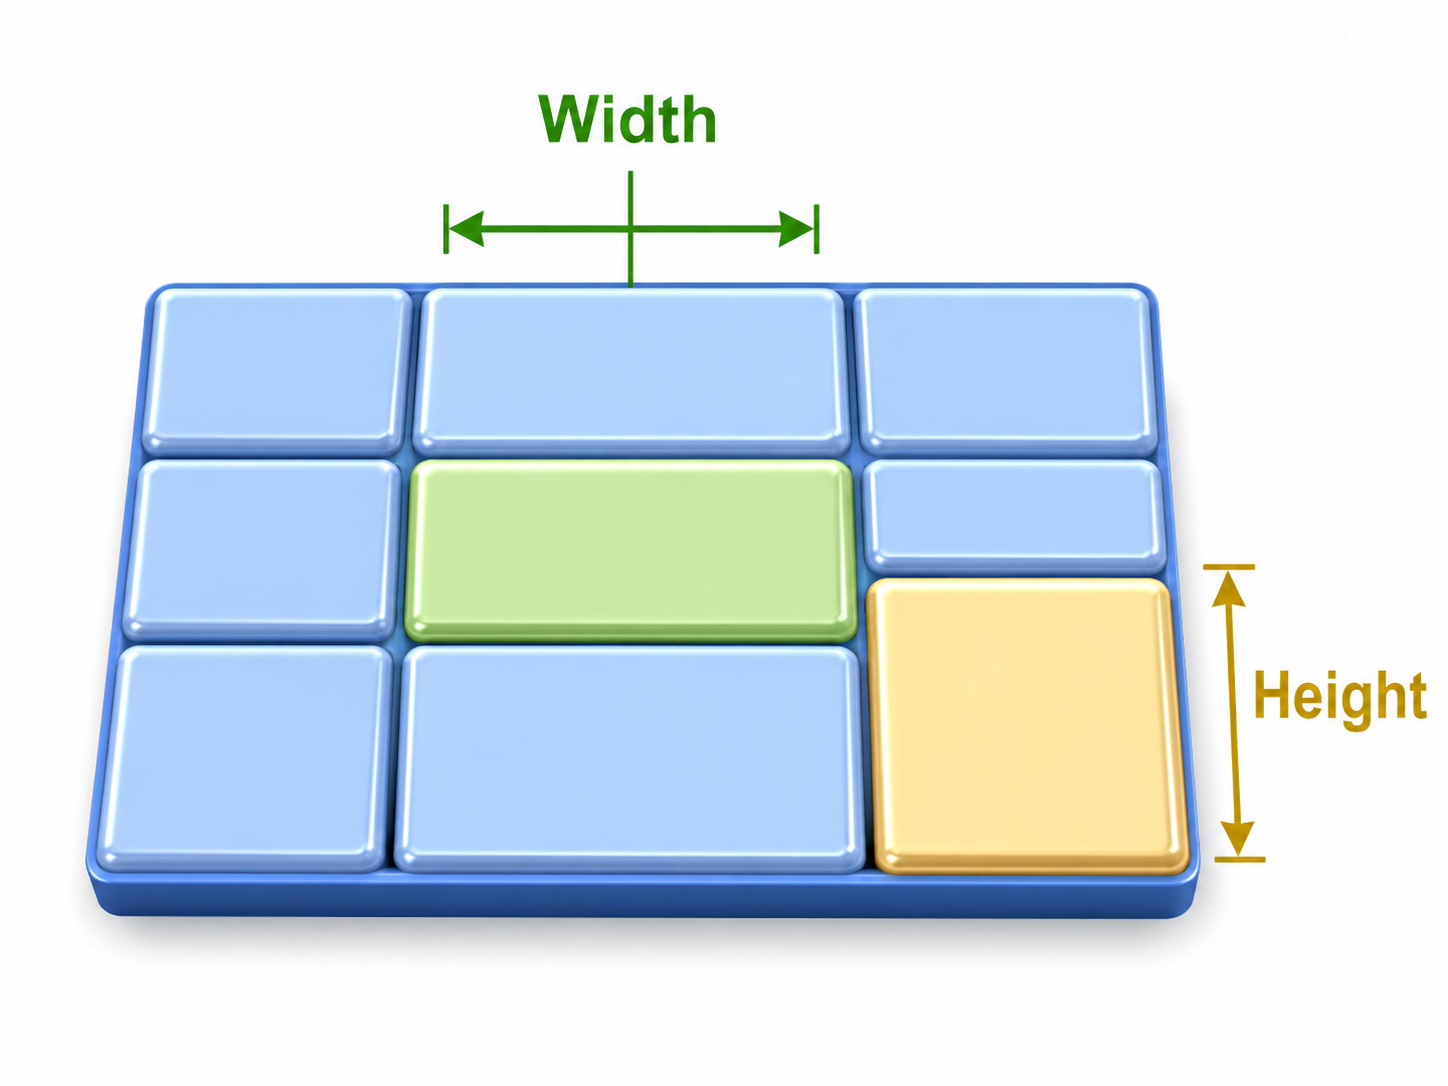
\includegraphics[width=0.95\linewidth,height=0.11\textheight,keepaspectratio]{chapters/Chapter04/topics/images/ex10_3d_cell_width_height.png}
}{
\fbox{\parbox{0.90\linewidth}{\centering\vspace{0.4cm}
\textbf{চিত্র}\\
File: \texttt{chapters/Chapter04/topics/images/ex10\_3d\_cell\_width\_height.png}
\vspace{0.4cm}}}
}
\captionof{figure}{Exercise 10-এর width-height চিত্র}
\end{center}

\begin{keypointbox}{চিত্র ব্যাখ্যা}
চিত্রে একটি table-এর মাঝের cell-এ width বেশি এবং ডান দিকের নিচের cell-এ height বেশি দেখানো হয়েছে।
\end{keypointbox}

\begin{keypointbox}{চিত্র দেখে code লেখার ধাপ}
যে cell চওড়া হবে সেখানে \texttt{width} attribute এবং যে cell লম্বা হবে সেখানে \texttt{height} attribute বসাবে।
\end{keypointbox}

\par\noindent{\color{purple!70!black}\bfseries\small কোড}\par\vspace{-4pt}
\begin{verbatim}
<!DOCTYPE html>
<html>
<head>
  <title>HTML Table Example</title>
</head>
<body>
<table border="1" cellspacing="0" cellpadding="8">
  <tr><td>A1</td><td>A2</td><td>A3</td></tr>
  <tr><td>B1</td><td width="120">Wide Cell</td><td>B3</td></tr>
  <tr><td>C1</td><td>C2</td><td height="80">Tall Cell</td></tr>
</table>
</body>
</html>
\end{verbatim}
\vspace{-6pt}

\subsubsection{Exercise 11: Month Income Cost Table}

\begin{boardbox}{Concept}
\texttt{valign} attribute দিয়ে cell-এর content vertically top, middle বা bottom position-এ রাখা যায়।
\end{boardbox}

\begin{center}
\IfFileExists{chapters/Chapter04/topics/images/ex11_3d_valign_month_income_cost.png}{
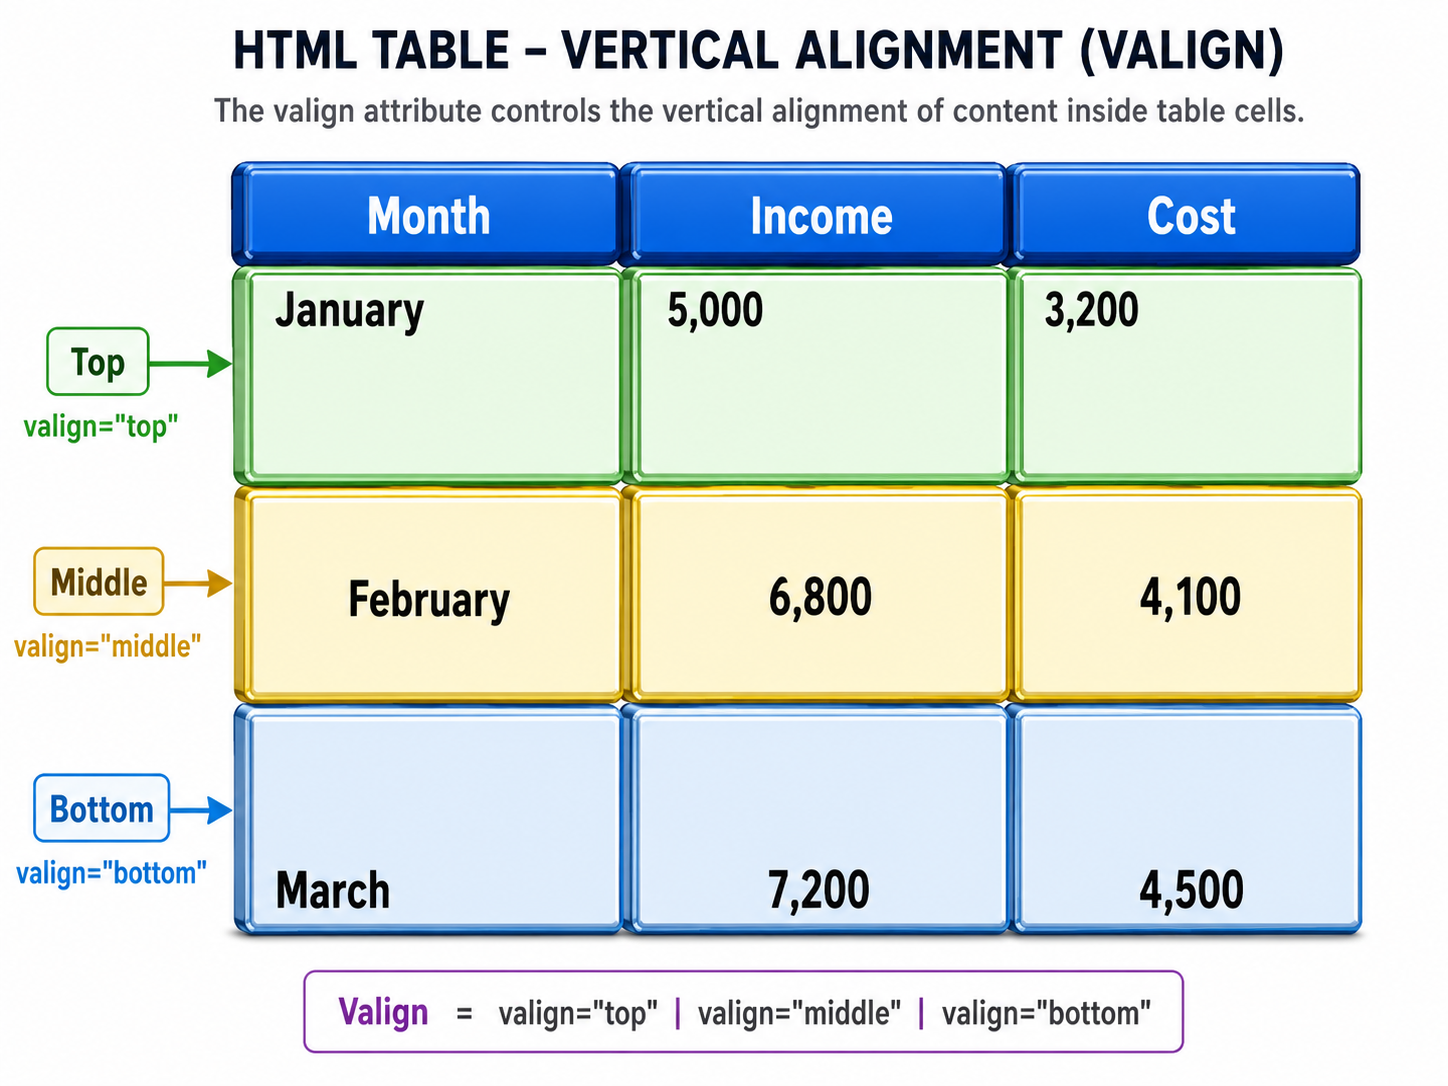
\includegraphics[width=0.95\linewidth,height=0.11\textheight,keepaspectratio]{chapters/Chapter04/topics/images/ex11_3d_valign_month_income_cost.png}
}{
\fbox{\parbox{0.90\linewidth}{\centering\vspace{0.4cm}
\textbf{চিত্র}\\
File: \texttt{chapters/Chapter04/topics/images/ex11\_3d\_valign\_month\_income\_cost.png}
\vspace{0.4cm}}}
}
\captionof{figure}{Exercise 11-এর valign চিত্র}
\end{center}

\begin{keypointbox}{চিত্র ব্যাখ্যা}
চিত্রে Month, Income ও Cost table দেখানো হয়েছে। January row top, February row middle এবং March row bottom vertical alignment বোঝায়।
\end{keypointbox}

\begin{keypointbox}{চিত্র দেখে code লেখার ধাপ}
প্রথম row-তে \texttt{valign="top"}, দ্বিতীয় row-তে \texttt{valign="middle"}, তৃতীয় row-তে \texttt{valign="bottom"} ব্যবহার করবে।
\end{keypointbox}

\par\noindent{\color{purple!70!black}\bfseries\small কোড}\par\vspace{-4pt}
\begin{verbatim}
<!DOCTYPE html>
<html>
<head>
  <title>HTML Table Example</title>
</head>
<body>
<table border="1" cellspacing="0" cellpadding="8">
  <tr><th>Month</th><th>Income</th><th>Cost</th></tr>
  <tr valign="top" height="60"><td>January</td><td>5,000</td><td>3,200</td></tr>
  <tr valign="middle" height="60"><td>February</td><td>6,800</td><td>4,100</td></tr>
  <tr valign="bottom" height="60"><td>March</td><td>7,200</td><td>4,500</td></tr>
</table>
</body>
</html>
\end{verbatim}
\vspace{-6pt}

\subsubsection{Exercise 12: Colgroup দিয়ে Column Color}

\begin{boardbox}{Concept}
\texttt{<colgroup>} ও \texttt{<col>} tag দিয়ে নির্দিষ্ট column-এর style দেওয়া যায়।
\end{boardbox}

\begin{center}
\IfFileExists{chapters/Chapter04/topics/images/ex12_3d_colgroup_color.png}{
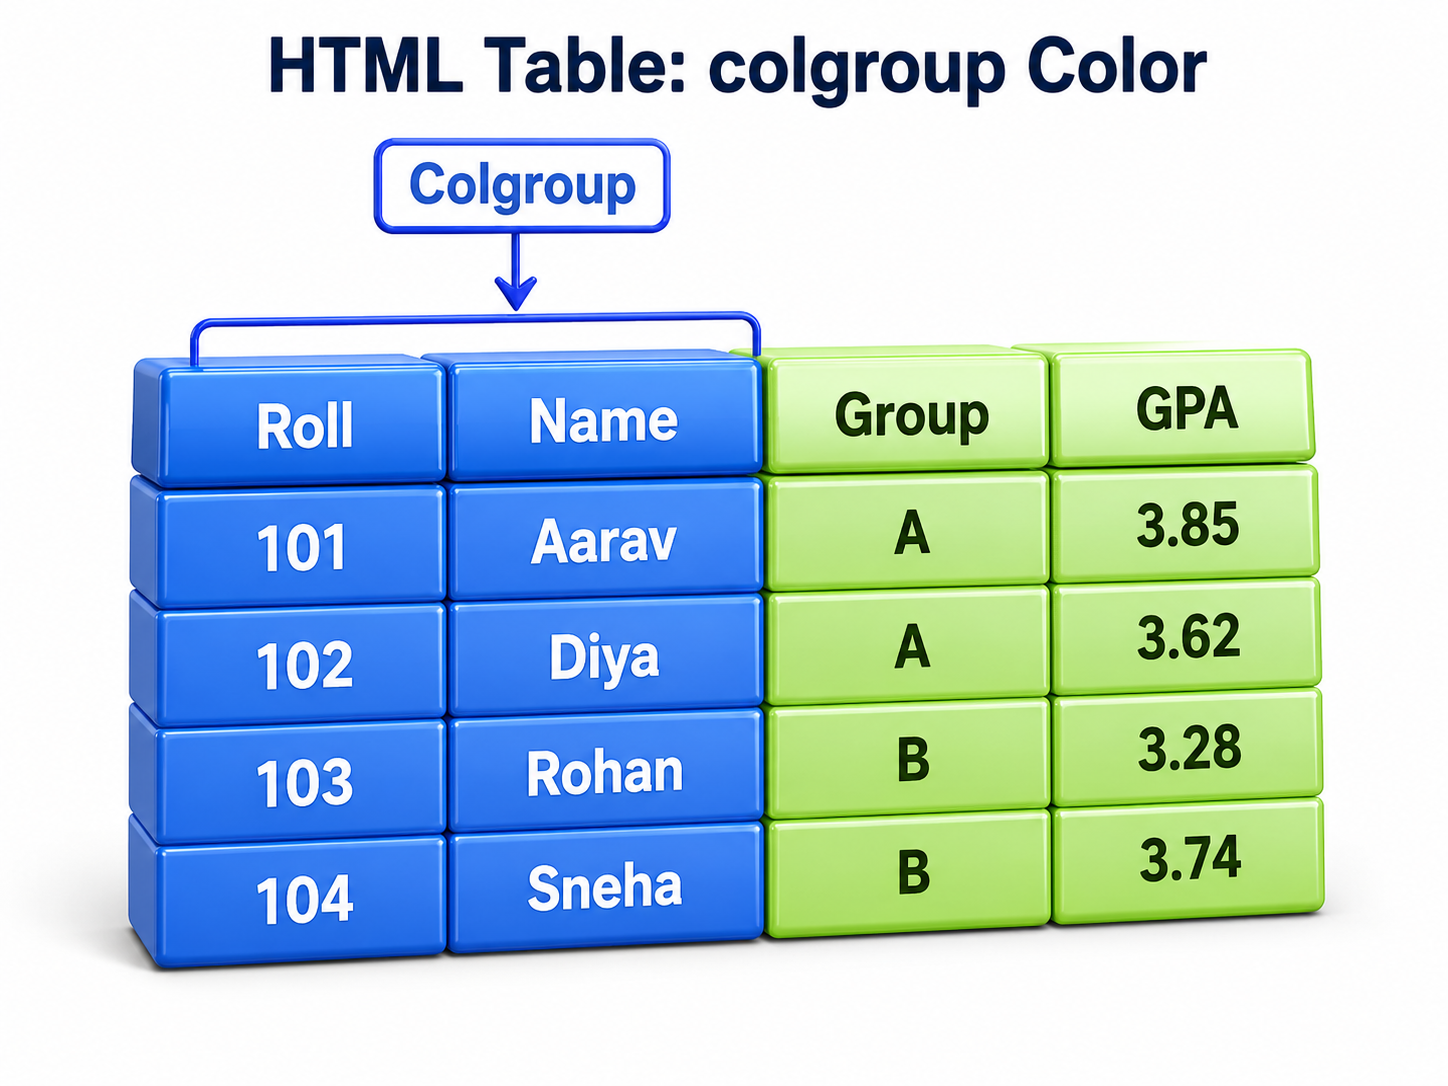
\includegraphics[width=0.95\linewidth,height=0.11\textheight,keepaspectratio]{chapters/Chapter04/topics/images/ex12_3d_colgroup_color.png}
}{
\fbox{\parbox{0.90\linewidth}{\centering\vspace{0.4cm}
\textbf{চিত্র}\\
File: \texttt{chapters/Chapter04/topics/images/ex12\_3d\_colgroup\_color.png}
\vspace{0.4cm}}}
}
\captionof{figure}{Exercise 12-এর colgroup চিত্র}
\end{center}

\begin{keypointbox}{চিত্র ব্যাখ্যা}
চিত্রে Roll ও Name column এক রঙে এবং Group ও GPA column আরেক রঙে দেখানো হয়েছে। এটি colgroup দিয়ে column-based styling বোঝায়।
\end{keypointbox}

\begin{keypointbox}{চিত্র দেখে code লেখার ধাপ}
প্রথমে \texttt{<colgroup>} লিখবে। কোন column কোন color হবে তা \texttt{<col span="...">} দিয়ে নির্ধারণ করবে। তারপর normal table row লিখবে।
\end{keypointbox}

\par\noindent{\color{purple!70!black}\bfseries\small কোড}\par\vspace{-4pt}
\begin{verbatim}
<!DOCTYPE html>
<html>
<head>
  <title>HTML Table Example</title>
</head>
<body>
<table border="1" cellspacing="0" cellpadding="6">
  <colgroup>
    <col span="2" style="background-color:#77b7ff">
    <col span="2" style="background-color:#b7ef7a">
  </colgroup>
  <tr><th>Roll</th><th>Name</th><th>Group</th><th>GPA</th></tr>
  <tr><td>101</td><td>Aarav</td><td>A</td><td>3.85</td></tr>
  <tr><td>102</td><td>Diya</td><td>A</td><td>3.62</td></tr>
  <tr><td>103</td><td>Rohan</td><td>B</td><td>3.28</td></tr>
  <tr><td>104</td><td>Sneha</td><td>B</td><td>3.74</td></tr>
</table>
</body>
</html>
\end{verbatim}
\vspace{-6pt}

\subsubsection{Exercise 13: Without Cellspacing and With Cellspacing}

\begin{boardbox}{Concept}
\texttt{cellspacing} cell-এর বাইরের gap বা cellগুলোর মাঝের distance নিয়ন্ত্রণ করে।
\end{boardbox}

\begin{center}
\IfFileExists{chapters/Chapter04/topics/images/ex13_3d_cellspacing_compare.png}{
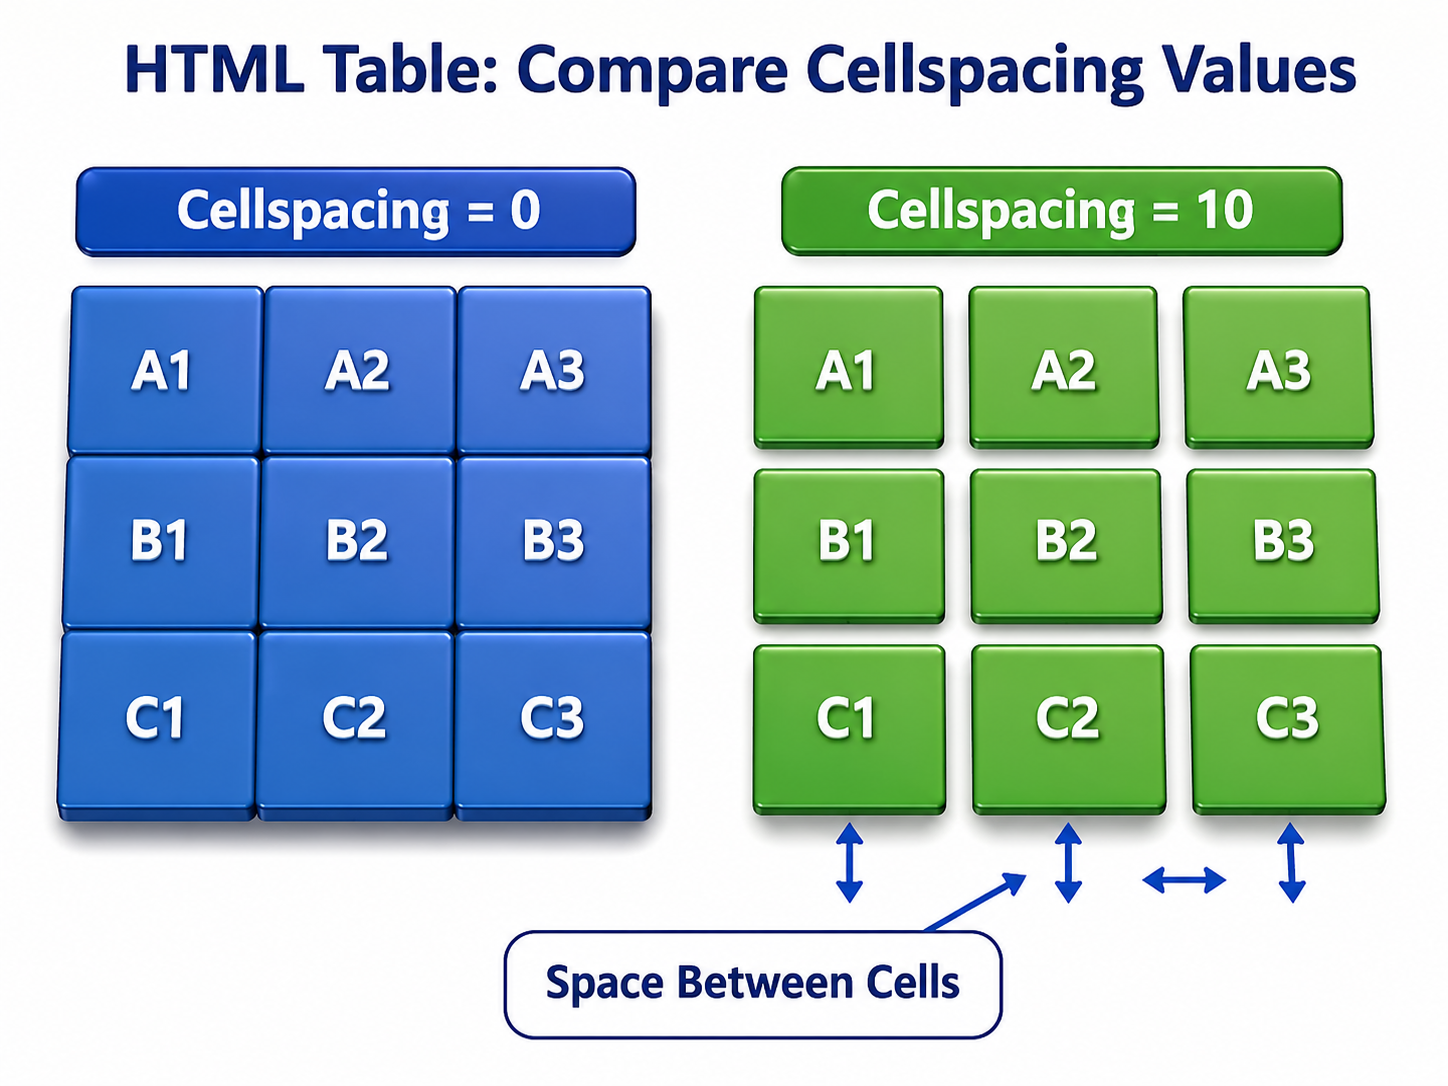
\includegraphics[width=0.95\linewidth,height=0.11\textheight,keepaspectratio]{chapters/Chapter04/topics/images/ex13_3d_cellspacing_compare.png}
}{
\fbox{\parbox{0.90\linewidth}{\centering\vspace{0.4cm}
\textbf{চিত্র}\\
File: \texttt{chapters/Chapter04/topics/images/ex13\_3d\_cellspacing\_compare.png}
\vspace{0.4cm}}}
}
\captionof{figure}{Exercise 13-এর cellspacing তুলনা}
\end{center}

\begin{keypointbox}{চিত্র ব্যাখ্যা}
চিত্রে বাম table-এ \texttt{cellspacing="0"} থাকায় cellগুলোর মাঝে gap নেই। ডান table-এ \texttt{cellspacing="10"} থাকায় cellগুলোর মাঝে space দেখা যাচ্ছে।
\end{keypointbox}

\begin{keypointbox}{চিত্র দেখে code লেখার ধাপ}
একই data দিয়ে দুটি table লিখবে। প্রথমটিতে \texttt{cellspacing="0"} এবং দ্বিতীয়টিতে \texttt{cellspacing="10"} ব্যবহার করবে।
\end{keypointbox}

\par\noindent{\color{purple!70!black}\bfseries\small কোড}\par\vspace{-4pt}
\begin{verbatim}
<!DOCTYPE html>
<html>
<head>
  <title>HTML Table Example</title>
</head>
<body>
<h3>Cellspacing = 0</h3>
<table border="1" cellspacing="0" cellpadding="8">
  <tr><td>A1</td><td>A2</td><td>A3</td></tr>
  <tr><td>B1</td><td>B2</td><td>B3</td></tr>
  <tr><td>C1</td><td>C2</td><td>C3</td></tr>
</table>

<h3>Cellspacing = 10</h3>
<table border="1" cellspacing="10" cellpadding="8">
  <tr><td>A1</td><td>A2</td><td>A3</td></tr>
  <tr><td>B1</td><td>B2</td><td>B3</td></tr>
  <tr><td>C1</td><td>C2</td><td>C3</td></tr>
</table>
</body>
</html>
\end{verbatim}
\vspace{-6pt}

\subsubsection{Exercise 14: Without Cellpadding and With Cellpadding}

\begin{boardbox}{Concept}
\texttt{cellpadding} cell-এর border এবং content-এর মাঝের ভিতরের space নিয়ন্ত্রণ করে।
\end{boardbox}

\begin{center}
\IfFileExists{chapters/Chapter04/topics/images/ex14_3d_cellpadding_compare.png}{
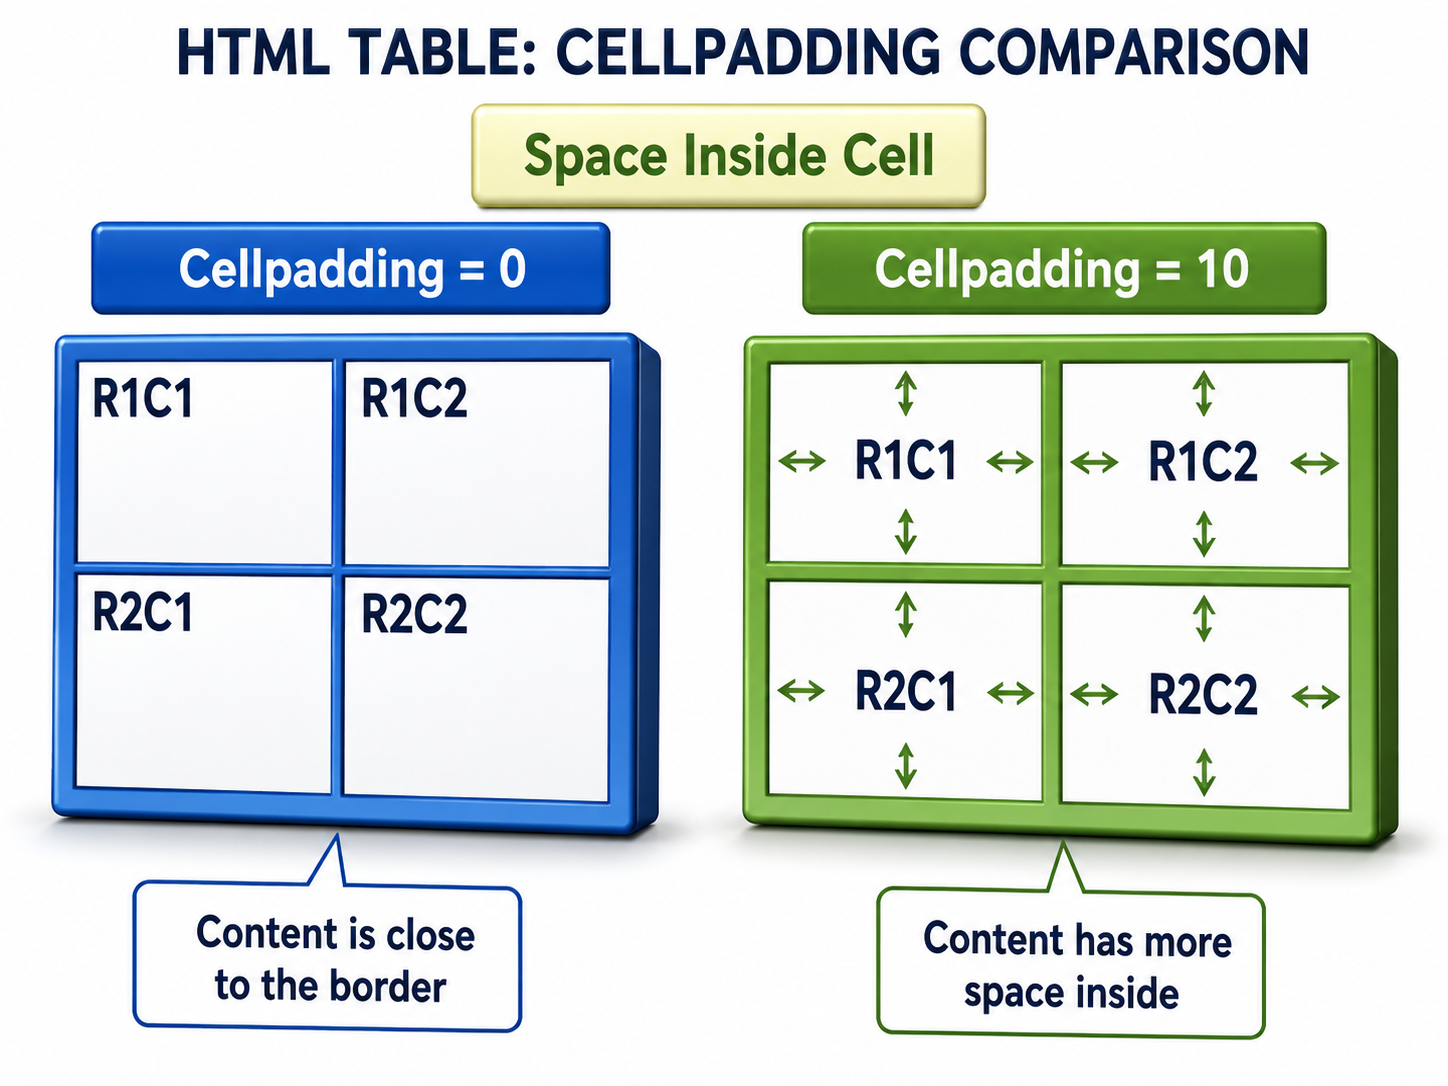
\includegraphics[width=0.95\linewidth,height=0.11\textheight,keepaspectratio]{chapters/Chapter04/topics/images/ex14_3d_cellpadding_compare.png}
}{
\fbox{\parbox{0.90\linewidth}{\centering\vspace{0.4cm}
\textbf{চিত্র}\\
File: \texttt{chapters/Chapter04/topics/images/ex14\_3d\_cellpadding\_compare.png}
\vspace{0.4cm}}}
}
\captionof{figure}{Exercise 14-এর cellpadding তুলনা}
\end{center}

\begin{keypointbox}{চিত্র ব্যাখ্যা}
চিত্রে বাম table-এ \texttt{cellpadding="0"} থাকায় content border-এর কাছে আছে। ডান table-এ \texttt{cellpadding="10"} থাকায় content-এর চারপাশে ভিতরের space বেশি।
\end{keypointbox}

\begin{keypointbox}{চিত্র দেখে code লেখার ধাপ}
দুটি table তৈরি করবে। প্রথম table-এ \texttt{cellpadding="0"}, দ্বিতীয় table-এ \texttt{cellpadding="10"} বসাবে।
\end{keypointbox}

\par\noindent{\color{purple!70!black}\bfseries\small কোড}\par\vspace{-4pt}
\begin{verbatim}
<!DOCTYPE html>
<html>
<head>
  <title>HTML Table Example</title>
</head>
<body>
<h3>Cellpadding = 0</h3>
<table border="1" cellspacing="0" cellpadding="0">
  <tr><td>R1C1</td><td>R1C2</td></tr>
  <tr><td>R2C1</td><td>R2C2</td></tr>
</table>

<h3>Cellpadding = 10</h3>
<table border="1" cellspacing="0" cellpadding="10">
  <tr><td>R1C1</td><td>R1C2</td></tr>
  <tr><td>R2C1</td><td>R2C2</td></tr>
</table>
</body>
</html>
\end{verbatim}
\vspace{-6pt}

\subsubsection{Exercise 15: Caption Tag Practice}

\begin{boardbox}{Concept}
\texttt{<caption>} table-এর উপরে title দেখায়। border value বাড়ালে border visually thick দেখায়।
\end{boardbox}

\begin{center}
\IfFileExists{chapters/Chapter04/topics/images/ex15_3d_caption_thick_border.png}{
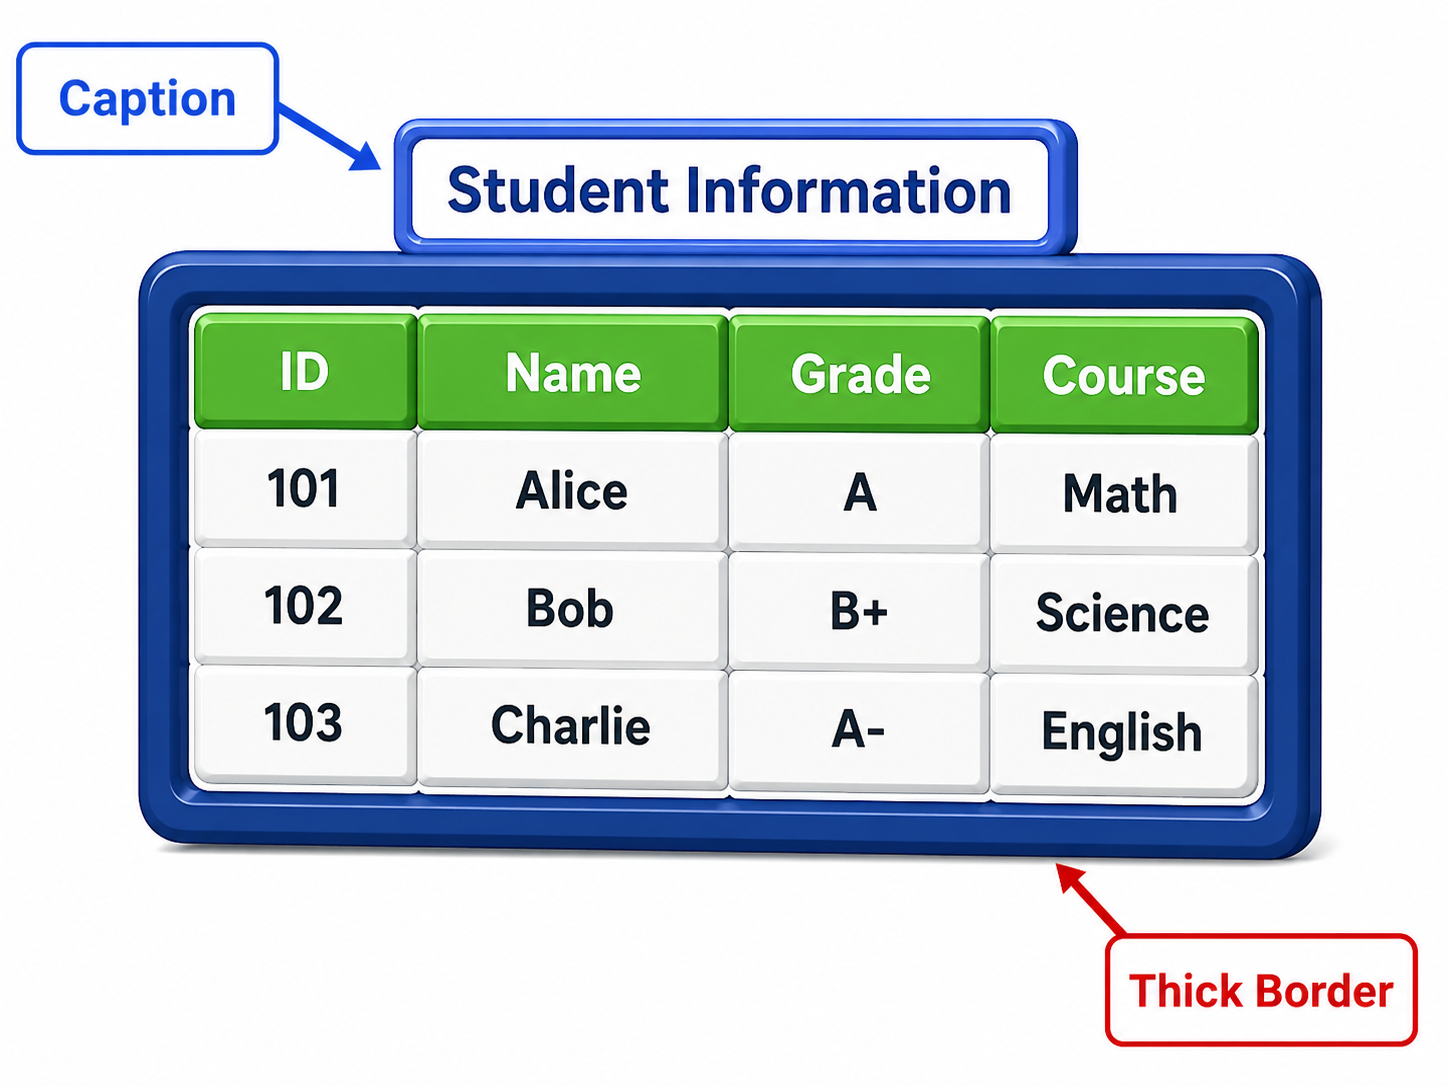
\includegraphics[width=0.95\linewidth,height=0.11\textheight,keepaspectratio]{chapters/Chapter04/topics/images/ex15_3d_caption_thick_border.png}
}{
\fbox{\parbox{0.90\linewidth}{\centering\vspace{0.4cm}
\textbf{চিত্র}\\
File: \texttt{chapters/Chapter04/topics/images/ex15\_3d\_caption\_thick\_border.png}
\vspace{0.4cm}}}
}
\captionof{figure}{Exercise 15-এর caption চিত্র}
\end{center}

\begin{keypointbox}{চিত্র ব্যাখ্যা}
চিত্রে Student Information caption এবং thick border সহ ID, Name, Grade ও Course column দেখানো হয়েছে।
\end{keypointbox}

\begin{keypointbox}{চিত্র দেখে code লেখার ধাপ}
প্রথমে table tag-এ border বসাবে। তারপর \texttt{<caption>} দিয়ে Student Information লিখবে। এরপর header row ও data rows লিখবে।
\end{keypointbox}

\par\noindent{\color{purple!70!black}\bfseries\small কোড}\par\vspace{-4pt}
\begin{verbatim}
<!DOCTYPE html>
<html>
<head>
  <title>HTML Table Example</title>
</head>
<body>
<table border="4" cellspacing="0" cellpadding="6">
  <caption><b>Student Information</b></caption>
  <tr><th>ID</th><th>Name</th><th>Grade</th><th>Course</th></tr>
  <tr><td>101</td><td>Alice</td><td>A</td><td>Math</td></tr>
  <tr><td>102</td><td>Bob</td><td>B+</td><td>Science</td></tr>
  <tr><td>103</td><td>Charlie</td><td>A-</td><td>English</td></tr>
</table>
</body>
</html>
\end{verbatim}
\vspace{-6pt}

\subsubsection{Exercise 16: Bio-data Table with Next Link}

\begin{boardbox}{Concept}
Table cell-এর ভিতরে hyperlink রাখা যায়। Bio-data table-এ label এবং value দুই column হিসেবে সাজানো হয়।
\end{boardbox}

\begin{center}
\IfFileExists{chapters/Chapter04/topics/images/ex16_3d_biodata_link.png}{
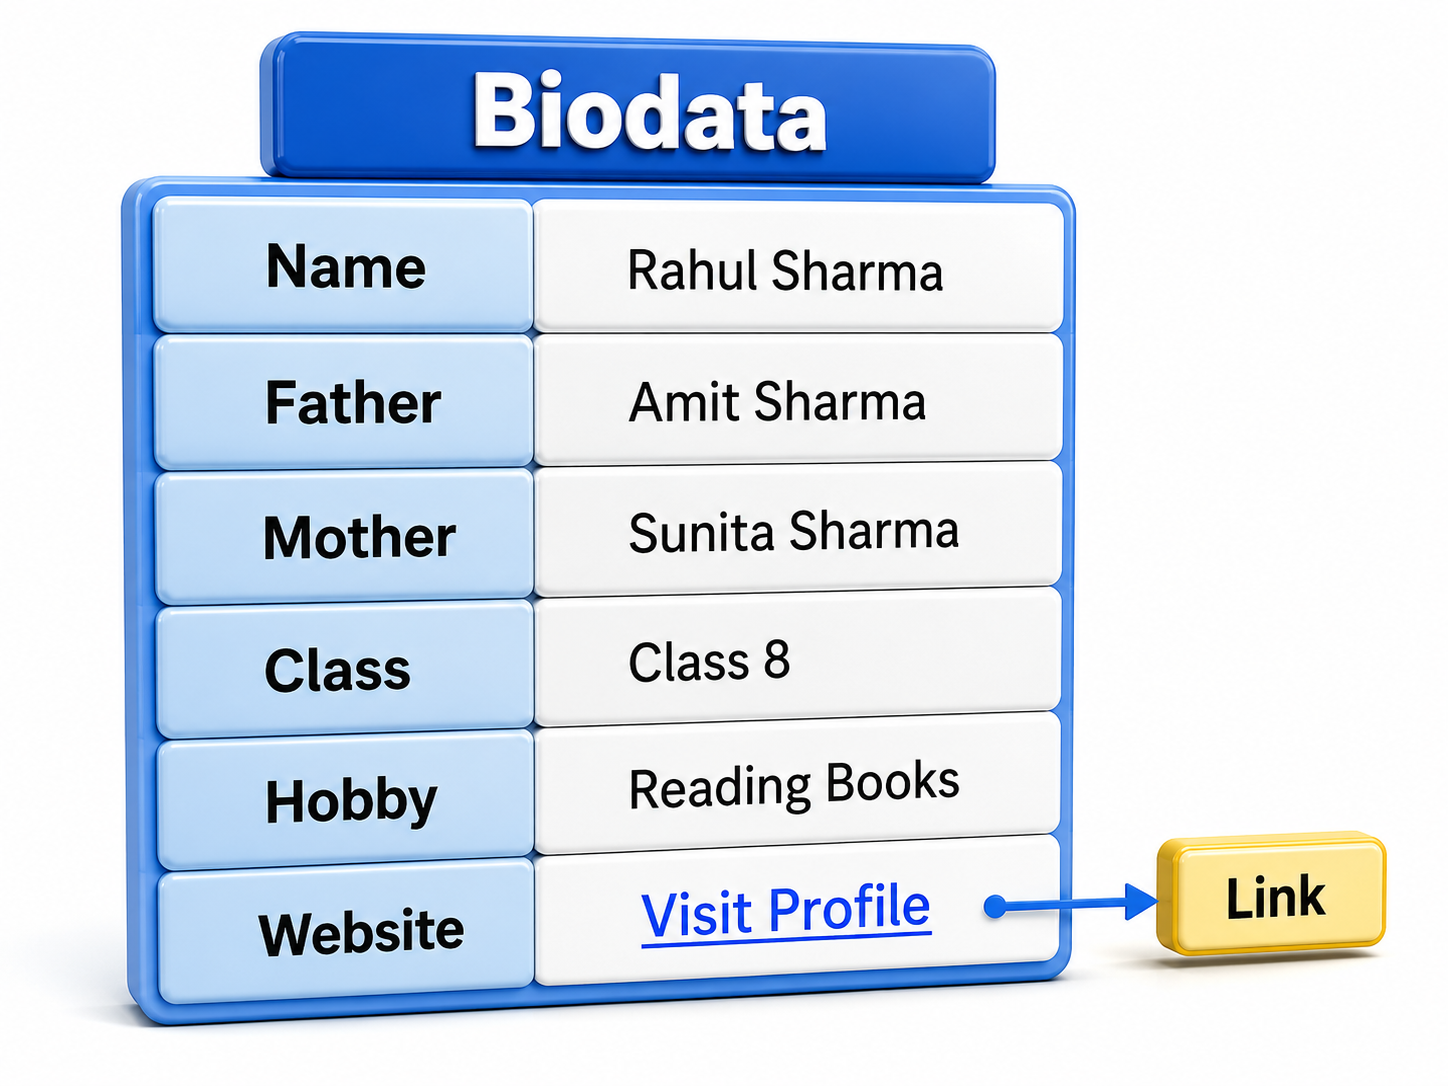
\includegraphics[width=0.95\linewidth,height=0.11\textheight,keepaspectratio]{chapters/Chapter04/topics/images/ex16_3d_biodata_link.png}
}{
\fbox{\parbox{0.90\linewidth}{\centering\vspace{0.4cm}
\textbf{চিত্র}\\
File: \texttt{chapters/Chapter04/topics/images/ex16\_3d\_biodata\_link.png}
\vspace{0.4cm}}}
}
\captionof{figure}{Exercise 16-এর biodata table চিত্র}
\end{center}

\begin{keypointbox}{চিত্র ব্যাখ্যা}
চিত্রে Biodata heading-এর নিচে Name, Father, Mother, Class, Hobby এবং Website row আছে। Website row-তে Visit Profile hyperlink দেখানো হয়েছে।
\end{keypointbox}

\begin{keypointbox}{চিত্র দেখে code লেখার ধাপ}
প্রথমে title row দুই column জুড়ে দিতে \texttt{colspan="2"} ব্যবহার করবে। তারপর প্রতিটি label-value row লিখবে। Website cell-এ \texttt{<a>} tag দিয়ে link তৈরি করবে।
\end{keypointbox}

\par\noindent{\color{purple!70!black}\bfseries\small কোড}\par\vspace{-4pt}
\begin{verbatim}
<!DOCTYPE html>
<html>
<head>
  <title>HTML Table Example</title>
</head>
<body>
<table border="1" cellspacing="0" cellpadding="6" align="center">
  <tr><th colspan="2">Biodata</th></tr>
  <tr><th>Name</th><td>Rahul Sharma</td></tr>
  <tr><th>Father</th><td>Amit Sharma</td></tr>
  <tr><th>Mother</th><td>Sunita Sharma</td></tr>
  <tr><th>Class</th><td>Class 8</td></tr>
  <tr><th>Hobby</th><td>Reading Books</td></tr>
  <tr><th>Website</th><td><a href="profile.html">Visit Profile</a></td></tr>
</table>
</body>
</html>
\end{verbatim}
\vspace{-6pt}
\subsubsection{Exercise 17: Mobile Company Table}

\begin{center}
\IfFileExists{chapters/Chapter04/topics/images/ex17_3d_mobile_company.png}{
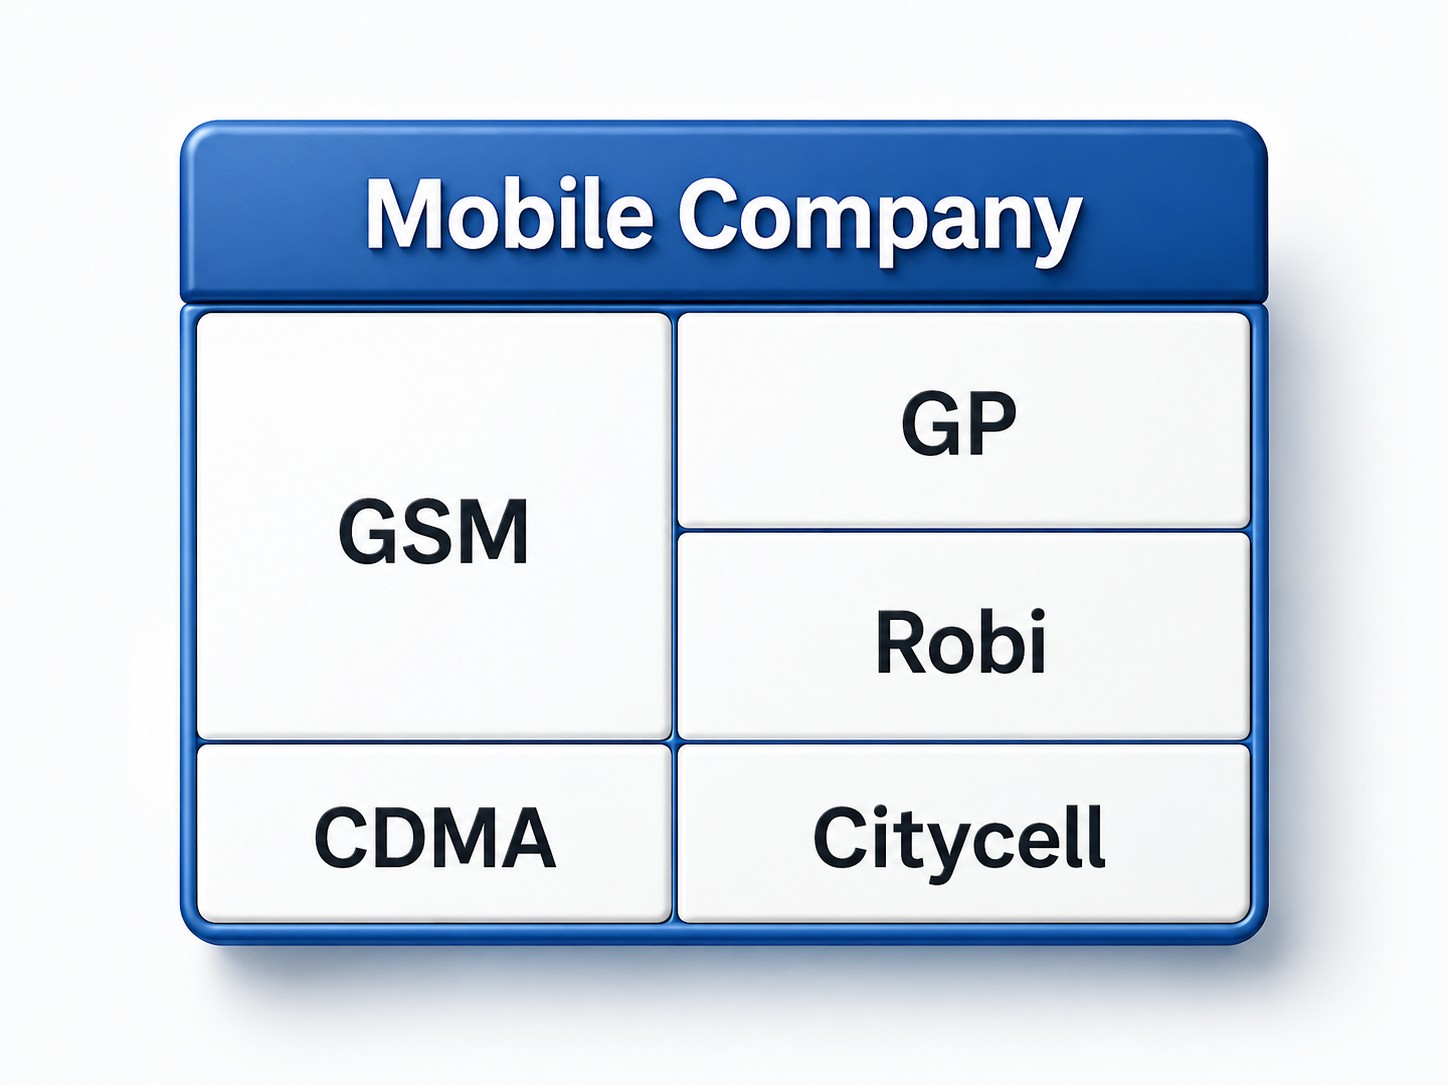
\includegraphics[width=0.95\linewidth,height=0.11\textheight,keepaspectratio]{chapters/Chapter04/topics/images/ex17_3d_mobile_company.png}
}{
\fbox{\parbox{0.90\linewidth}{\centering\vspace{0.45cm}
\textbf{চিত্র}\\[3pt]
File: \texttt{chapters/Chapter04/topics/images/ex17\_3d\_mobile\_company.png}
\vspace{0.45cm}}}
}
\captionof{figure}{Mobile Company table with rowspan}
\end{center}

\begin{keypointbox}{চিত্র ব্যাখ্যা}
GSM cell দুই row জুড়ে আছে। তাই GP ও Robi একই GSM category-এর অধীনে দেখানো হয়েছে। CDMA ও Citycell শেষ row-তে আছে।
\end{keypointbox}

\begin{keypointbox}{চিত্র দেখে code লেখার ধাপ}
প্রথমে figure-এর total row ও column গুনবে। এরপর কোন cell একাধিক column জুড়ে আছে তা দেখে \texttt{colspan} এবং কোন cell একাধিক row জুড়ে আছে তা দেখে \texttt{rowspan} বসাবে। তারপর image, link, list বা nested table থাকলে সংশ্লিষ্ট tag cell-এর ভিতরে লিখবে।
\end{keypointbox}

\par\noindent{\color{purple!70!black}\bfseries\small কোড}\par\vspace{-4pt}
\begin{verbatim}
<!DOCTYPE html>
<html>
<head>
  <title>HTML Table Example</title>
</head>
<body>
<table border="1" cellspacing="0">
<caption>Mobile Company</caption>
<tr>
  <td rowspan="2">GSM</td>
  <td>GP</td>
</tr>
<tr>
  <td>Robi</td>
</tr>
<tr>
  <td>CDMA</td>
  <td>Citycell</td>
</tr>
</table>
</body>
</html>
\end{verbatim}
\vspace{-6pt}

\subsubsection{Exercise 18: Complex Number Grid with Rowspan and Colspan}

\begin{center}
\IfFileExists{chapters/Chapter04/topics/images/ex18_3d_complex_number_grid.png}{
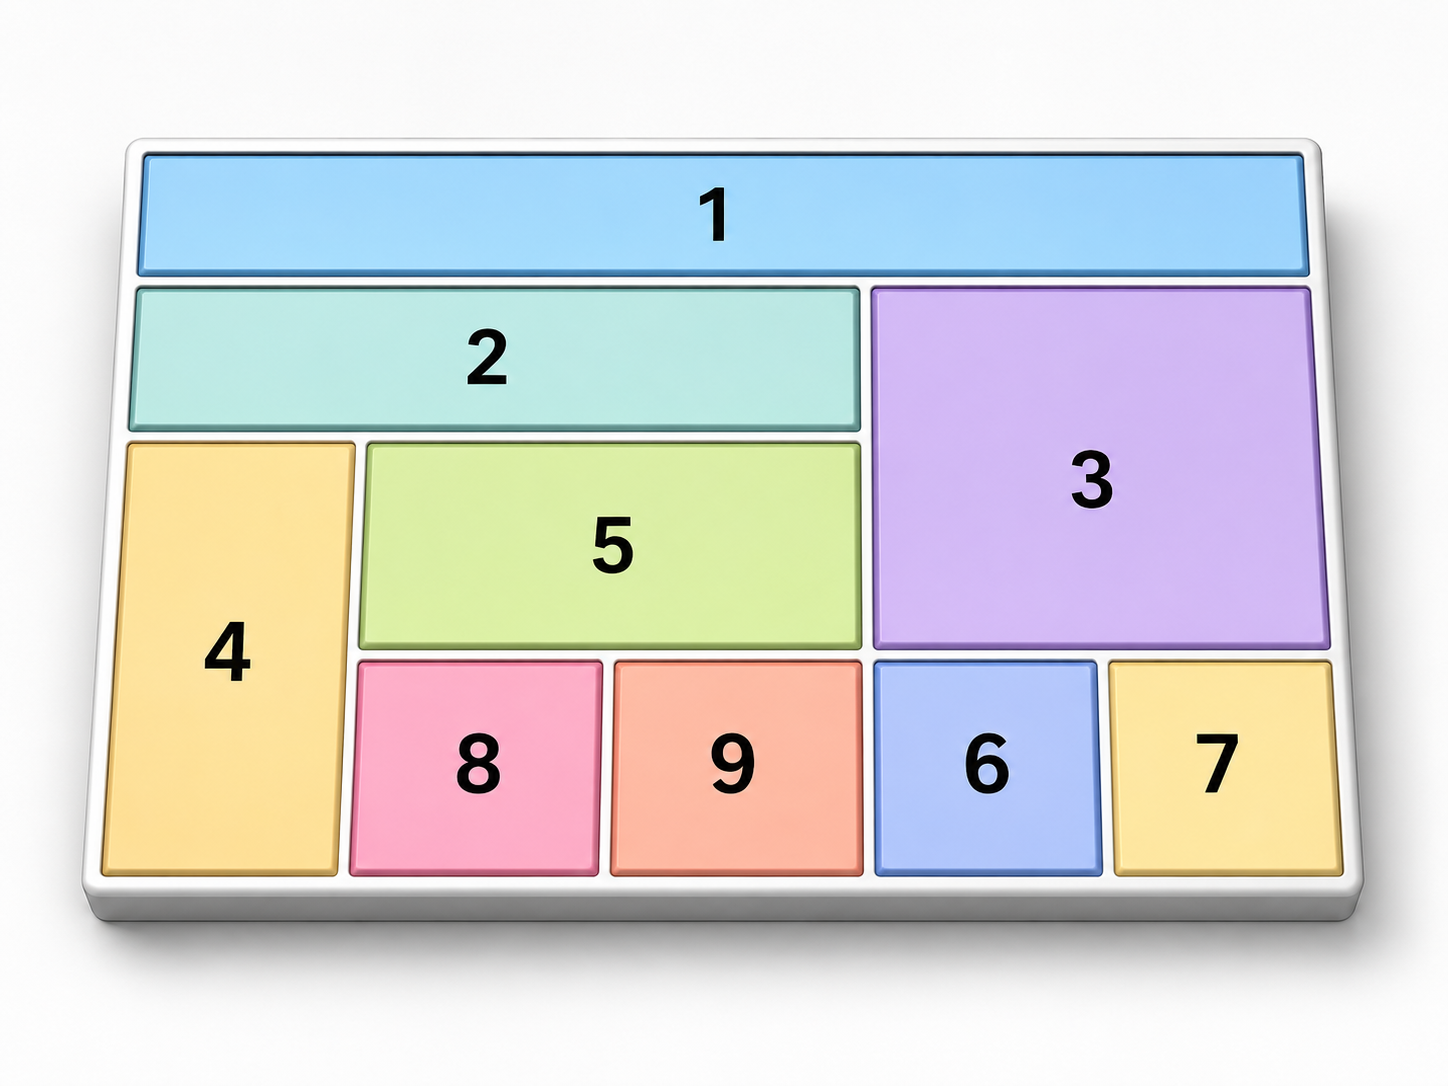
\includegraphics[width=0.95\linewidth,height=0.11\textheight,keepaspectratio]{chapters/Chapter04/topics/images/ex18_3d_complex_number_grid.png}
}{
\fbox{\parbox{0.90\linewidth}{\centering\vspace{0.45cm}
\textbf{চিত্র}\\[3pt]
File: \texttt{chapters/Chapter04/topics/images/ex18\_3d\_complex\_number\_grid.png}
\vspace{0.45cm}}}
}
\captionof{figure}{Complex number grid with rowspan and colspan}
\end{center}

\begin{keypointbox}{চিত্র ব্যাখ্যা}
এই table-এ 1, 2, 3, 4, 5, 8, 9 cell-এ rowspan/colspan ব্যবহার করা হয়েছে। চিত্র দেখে code লেখার জন্য এটি খুব গুরুত্বপূর্ণ practice।
\end{keypointbox}

\par\noindent{\color{purple!70!black}\bfseries\small কোড}\par\vspace{-4pt}
\begin{verbatim}
<!DOCTYPE html>
<html>
<head>
  <title>HTML Table Example</title>
</head>
<body>
<table border="1" cellspacing="0">
<tr><td colspan="5">1</td></tr>
<tr><td colspan="3">2</td><td colspan="2" rowspan="3">3</td></tr>
<tr><td rowspan="3">4</td><td colspan="2">5</td></tr>
<tr><td rowspan="2">8</td><td rowspan="2">9</td></tr>
<tr><td>6</td><td>7</td></tr>
</table>
</body>
</html>
\end{verbatim}
\vspace{-6pt}

\subsubsection{Exercise 19: Mymensingh Gov. College Group and Seats Table}

\begin{center}
\IfFileExists{chapters/Chapter04/topics/images/ex19_3d_mgc_group_seats.png}{
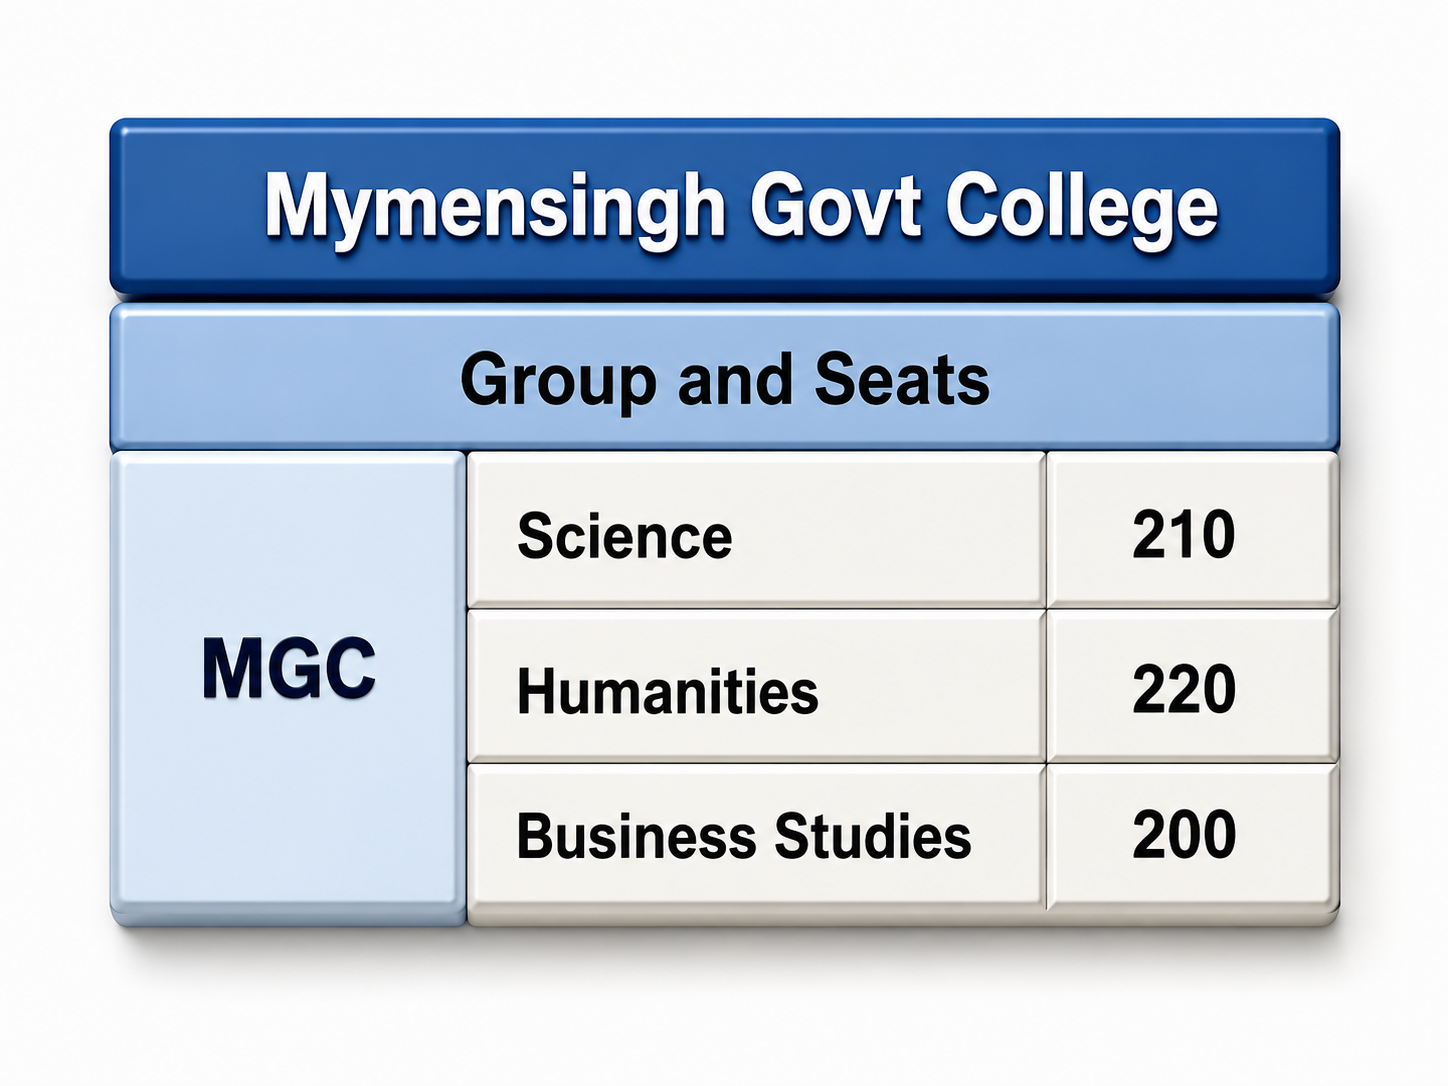
\includegraphics[width=0.95\linewidth,height=0.11\textheight,keepaspectratio]{chapters/Chapter04/topics/images/ex19_3d_mgc_group_seats.png}
}{
\fbox{\parbox{0.90\linewidth}{\centering\vspace{0.45cm}
\textbf{চিত্র}\\[3pt]
File: \texttt{chapters/Chapter04/topics/images/ex19\_3d\_mgc\_group\_seats.png}
\vspace{0.45cm}}}
}
\captionof{figure}{Mymensingh Govt. College group and seats table}
\end{center}

\begin{keypointbox}{চিত্র ব্যাখ্যা}
MGC cell তিনটি group row জুড়ে আছে। Group and Seats heading তিনটি column জুড়ে আছে।
\end{keypointbox}

\begin{keypointbox}{চিত্র দেখে code লেখার ধাপ}
প্রথমে figure-এর total row ও column গুনবে। এরপর কোন cell একাধিক column জুড়ে আছে তা দেখে \texttt{colspan} এবং কোন cell একাধিক row জুড়ে আছে তা দেখে \texttt{rowspan} বসাবে। তারপর image, link, list বা nested table থাকলে সংশ্লিষ্ট tag cell-এর ভিতরে লিখবে।
\end{keypointbox}

\par\noindent{\color{purple!70!black}\bfseries\small কোড}\par\vspace{-4pt}
\begin{verbatim}
<!DOCTYPE html>
<html>
<head>
  <title>HTML Table Example</title>
</head>
<body>
<p align="center"><h2>Mymensingh Govt College</h2></p>
<table border="1" cellspacing="0" cellpadding="10">
<tr><th colspan="3">Group and Seats</th></tr>
<tr><td rowspan="3">MGC</td><td>Science</td><td>210</td></tr>
<tr><td>Humanities</td><td>220</td></tr>
<tr><td>Business Studies</td><td>200</td></tr>
</table>
</body>
</html>
\end{verbatim}
\vspace{-6pt}

\subsubsection{Exercise 20: Product Table with Image}

\begin{center}
\IfFileExists{chapters/Chapter04/topics/images/ex20_3d_product_image.png}{
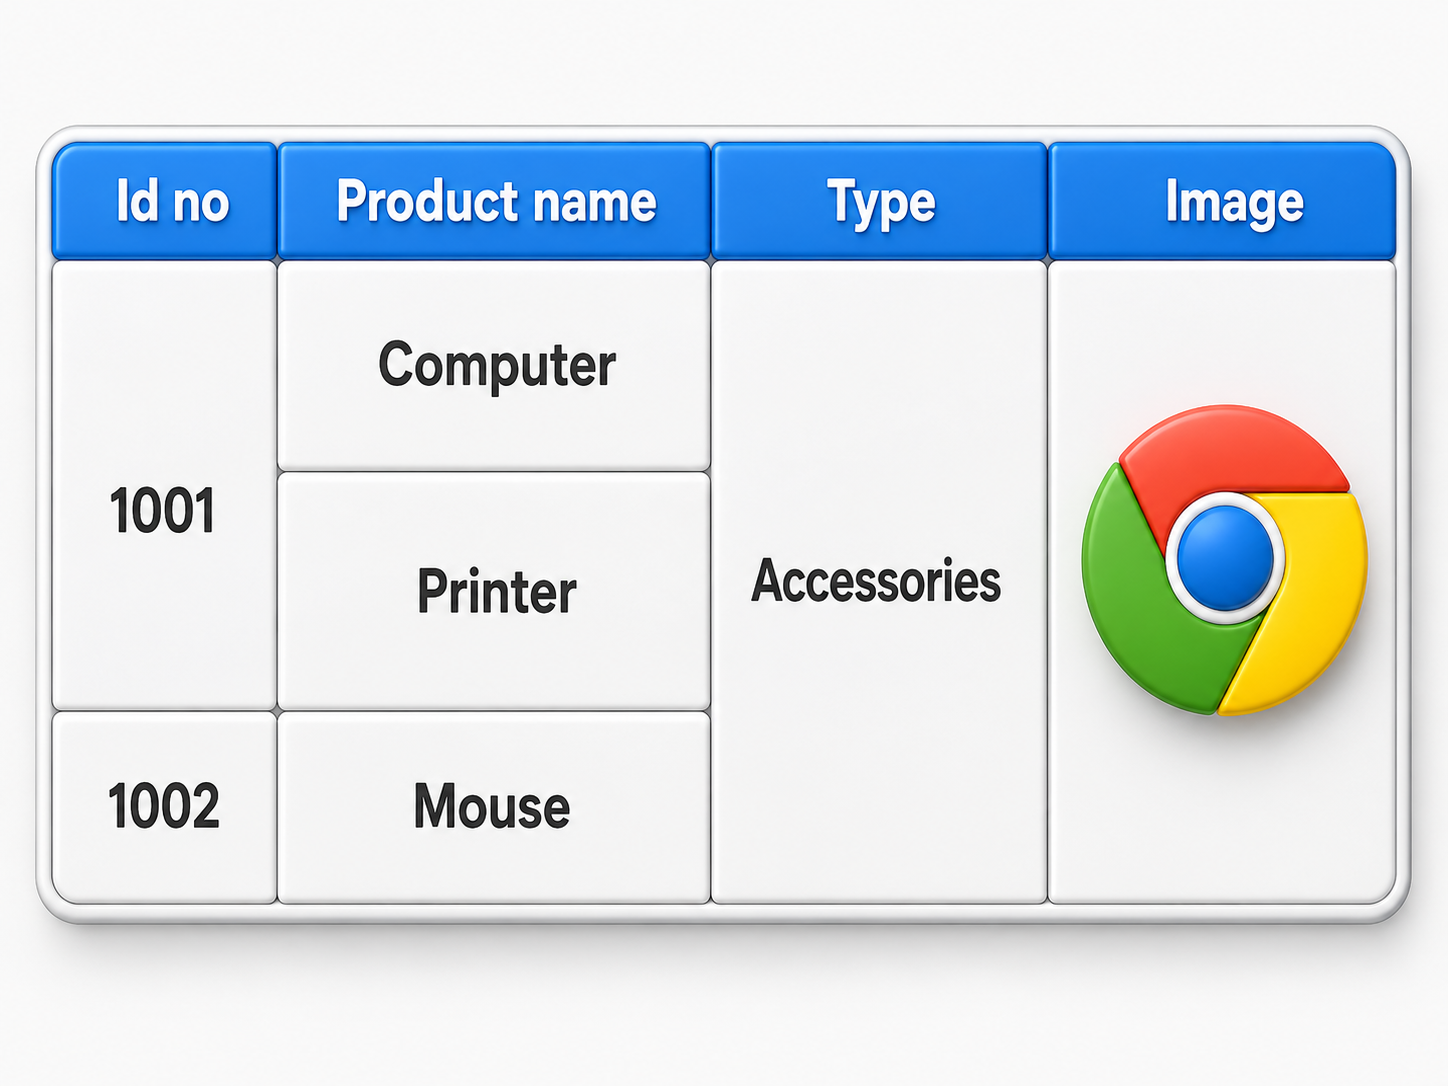
\includegraphics[width=0.95\linewidth,height=0.11\textheight,keepaspectratio]{chapters/Chapter04/topics/images/ex20_3d_product_image.png}
}{
\fbox{\parbox{0.90\linewidth}{\centering\vspace{0.45cm}
\textbf{চিত্র}\\[3pt]
File: \texttt{chapters/Chapter04/topics/images/ex20\_3d\_product\_image.png}
\vspace{0.45cm}}}
}
\captionof{figure}{Product table with rowspan and image}
\end{center}

\begin{keypointbox}{চিত্র ব্যাখ্যা}
এই table-এ image column-এর header cell চার row জুড়ে আছে। 1001 ID দুই product row জুড়ে এবং Accessories type তিন product row জুড়ে আছে।
\end{keypointbox}

\par\noindent{\color{purple!70!black}\bfseries\small কোড}\par\vspace{-4pt}
\begin{verbatim}
<!DOCTYPE html>
<html>
<head>
  <title>HTML Table Example</title>
</head>
<body>
<table border="1" cellspacing="0">
<tr>
  <th bgcolor="Silver">Id no</th>
  <th bgcolor="Silver">Product name</th>
  <th bgcolor="Silver">Type</th>
  <th rowspan="4"><img src="google.jpg" width="60" height="50" align="center"></th>
</tr>
<tr>
  <td rowspan="2">1001</td>
  <td>Computer</td>
  <td rowspan="3">Accessories</td>
</tr>
<tr>
  <td>Printer</td>
</tr>
<tr>
  <td>1002</td>
  <td>Mouse</td>
</tr>
</table>
</body>
</html>
\end{verbatim}
\vspace{-6pt}

\subsubsection{Exercise 21: Bangladesh Number Table}

\begin{center}
\IfFileExists{chapters/Chapter04/topics/images/ex21_3d_bangladesh_number_table.png}{
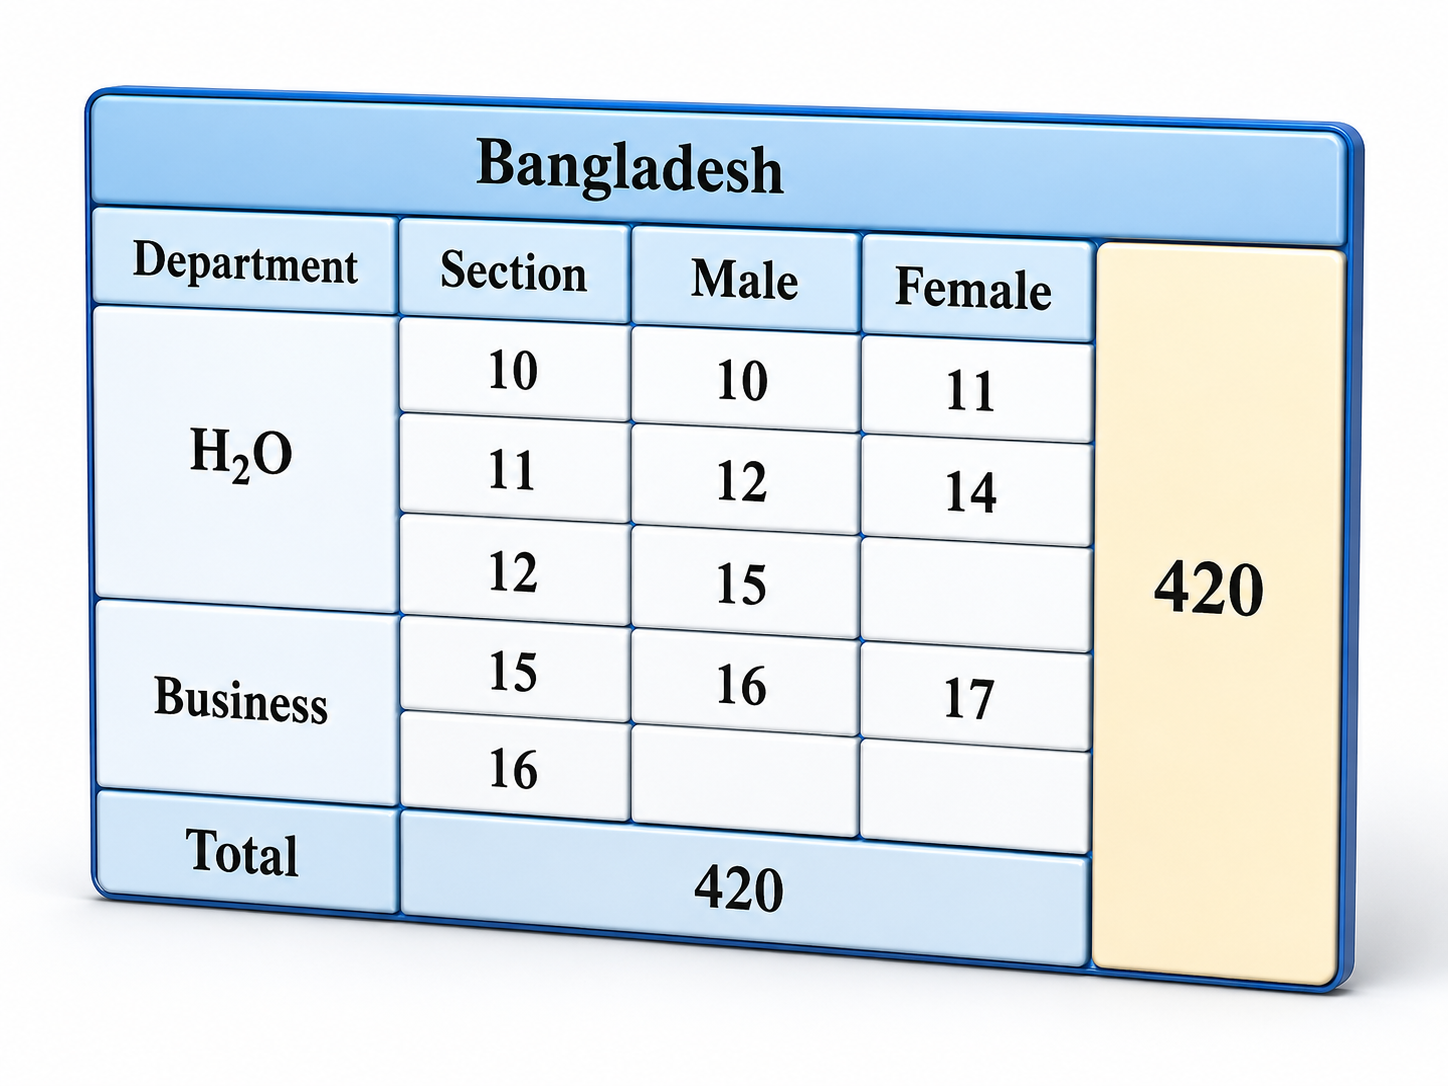
\includegraphics[width=0.95\linewidth,height=0.11\textheight,keepaspectratio]{chapters/Chapter04/topics/images/ex21_3d_bangladesh_number_table.png}
}{
\fbox{\parbox{0.90\linewidth}{\centering\vspace{0.45cm}
\textbf{চিত্র}\\[3pt]
File: \texttt{chapters/Chapter04/topics/images/ex21\_3d\_bangladesh\_number\_table.png}
\vspace{0.45cm}}}
}
\captionof{figure}{Bangladesh department number table with rowspan and colspan}
\end{center}

\begin{keypointbox}{চিত্র ব্যাখ্যা}
চিত্রে Bangladesh নামে একটি department-wise number table আছে। ডান পাশের \texttt{420} cell পুরো data অংশ জুড়ে আছে, তাই এখানে \texttt{rowspan} ব্যবহার করা হয়েছে। নিচের Total row-তে total value একাধিক column জুড়ে দেখানো হয়েছে।
\end{keypointbox}

\begin{keypointbox}{চিত্র দেখে code লেখার ধাপ}
প্রথমে header row-এর column গুনবে: Department, Section, Male, Female এবং ডান পাশের total cell। এরপর H\textsubscript{2}O/Business অংশে কোন cell কয়েকটি row জুড়ে আছে তা দেখে \texttt{rowspan} বসাবে। শেষে Total row-তে wide cell দরকার হলে \texttt{colspan} ব্যবহার করবে।
\end{keypointbox}

\par\noindent{\color{purple!70!black}\bfseries\small কোড}\par\vspace{-4pt}
\begin{verbatim}
<!DOCTYPE html>
<html>
<head>
  <title>HTML Table Example</title>
</head>
<body>
<table border="1" cellspacing="0" cellpadding="6">
<tr>
  <th>Department</th>
  <th>Section</th>
  <th>Male</th>
  <th>Female</th>
  <th rowspan="6" align="center">420</th>
</tr>
<tr>
  <td rowspan="3">H<sub>2</sub>O</td>
  <td>10</td>
  <td>10</td>
  <td>11</td>
</tr>
<tr>
  <td>11</td>
  <td>12</td>
  <td>14</td>
</tr>
<tr>
  <td>12</td>
  <td>15</td>
  <td>17</td>
</tr>
<tr>
  <td>Business</td>
  <td>15</td>
  <td>16</td>
  <td>17</td>
</tr>
<tr>
  <td>Total</td>
  <td colspan="3" align="center">420</td>
</tr>
</table>
</body>
</html>
\end{verbatim}
\vspace{-6pt}

\subsubsection{Exercise 22: Group, Section and No. of Student Table}

\begin{center}
\IfFileExists{chapters/Chapter04/topics/images/ex22_3d_group_section_student.png}{
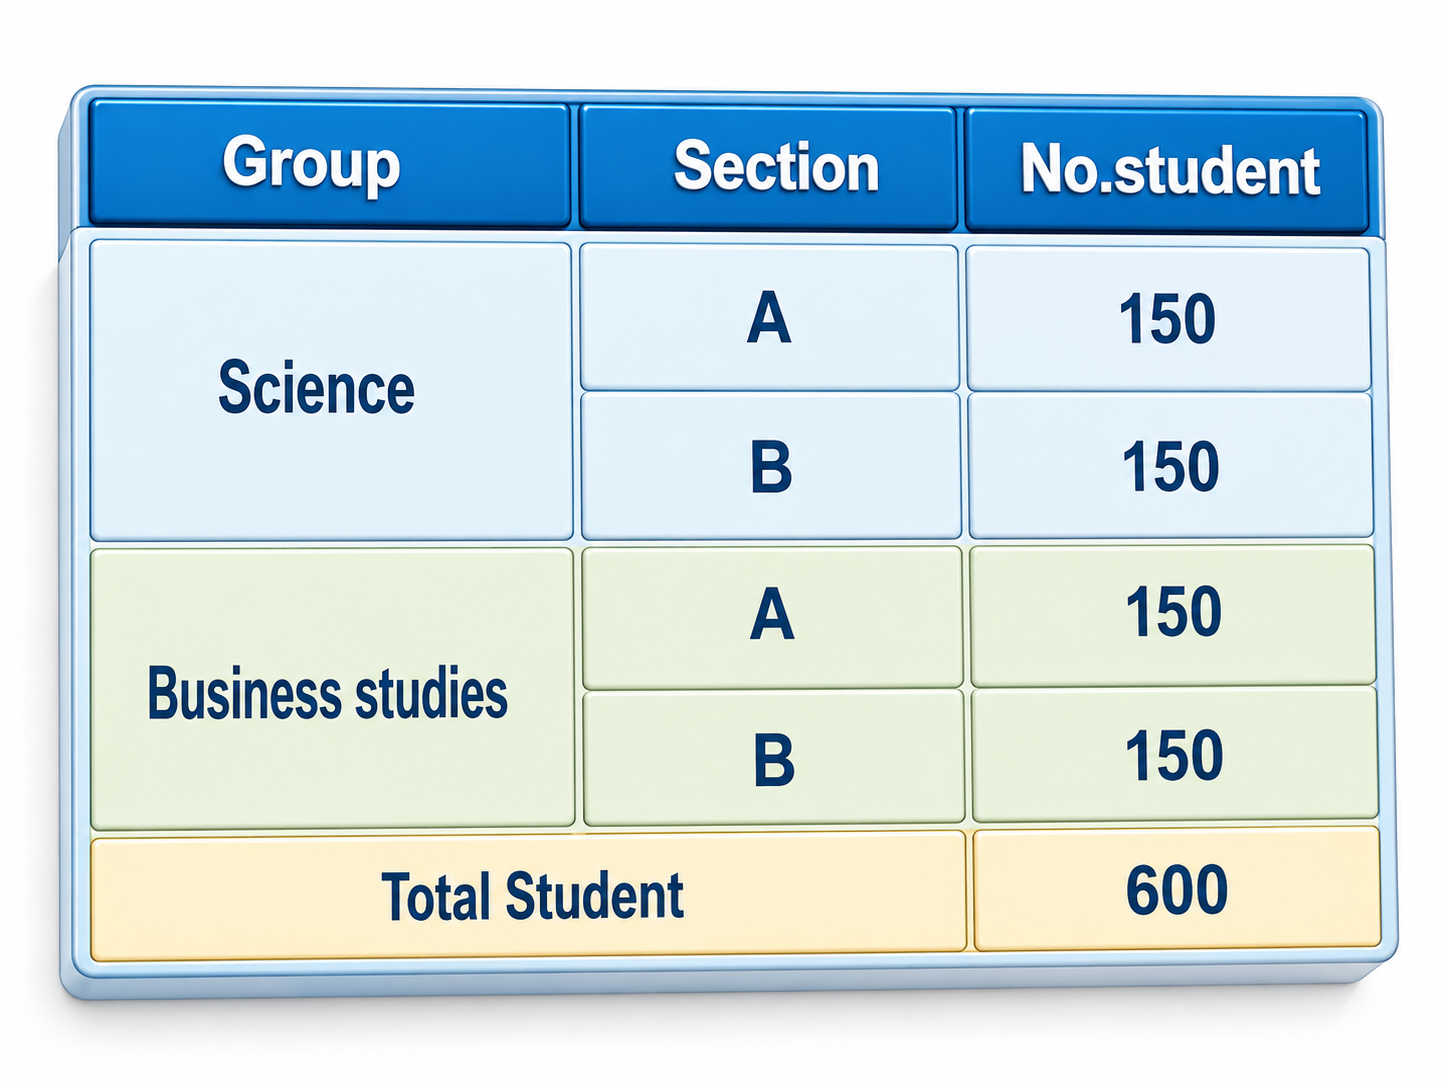
\includegraphics[width=0.95\linewidth,height=0.11\textheight,keepaspectratio]{chapters/Chapter04/topics/images/ex22_3d_group_section_student.png}
}{
\fbox{\parbox{0.90\linewidth}{\centering\vspace{0.45cm}
\textbf{চিত্র}\\[3pt]
File: \texttt{chapters/Chapter04/topics/images/ex22\_3d\_group\_section\_student.png}
\vspace{0.45cm}}}
}
\captionof{figure}{Group, Section and No. of student table}
\end{center}

\begin{keypointbox}{চিত্র ব্যাখ্যা}
Science এবং Business studies cell দুটি করে section row জুড়ে আছে। Total Student cell দুই column জুড়ে আছে।
\end{keypointbox}

\begin{keypointbox}{চিত্র দেখে code লেখার ধাপ}
প্রথমে figure-এর total row ও column গুনবে। এরপর কোন cell একাধিক column জুড়ে আছে তা দেখে \texttt{colspan} এবং কোন cell একাধিক row জুড়ে আছে তা দেখে \texttt{rowspan} বসাবে। তারপর image, link, list বা nested table থাকলে সংশ্লিষ্ট tag cell-এর ভিতরে লিখবে।
\end{keypointbox}

\par\noindent{\color{purple!70!black}\bfseries\small কোড}\par\vspace{-4pt}
\begin{verbatim}
<!DOCTYPE html>
<html>
<head>
  <title>HTML Table Example</title>
</head>
<body>
<table border="1" cellspacing="0">
<tr>
  <th>Group</th>
  <th>Section</th>
  <th>No. of student</th>
</tr>
<tr>
  <td rowspan="2">Science</td>
  <td>A</td>
  <td>150</td>
</tr>
<tr>
  <td>B</td>
  <td>150</td>
</tr>
<tr>
  <td rowspan="2">Business studies</td>
  <td>A</td>
  <td>150</td>
</tr>
<tr>
  <td>B</td>
  <td>150</td>
</tr>
<tr>
  <td colspan="2" align="center">Total student</td>
  <td>600</td>
</tr>
</table>
</body>
</html>
\end{verbatim}
\vspace{-6pt}

\subsubsection{Exercise 23: ID, Name and Contact No Table}

\begin{center}
\IfFileExists{chapters/Chapter04/topics/images/ex23_3d_contact_no_colspan.png}{
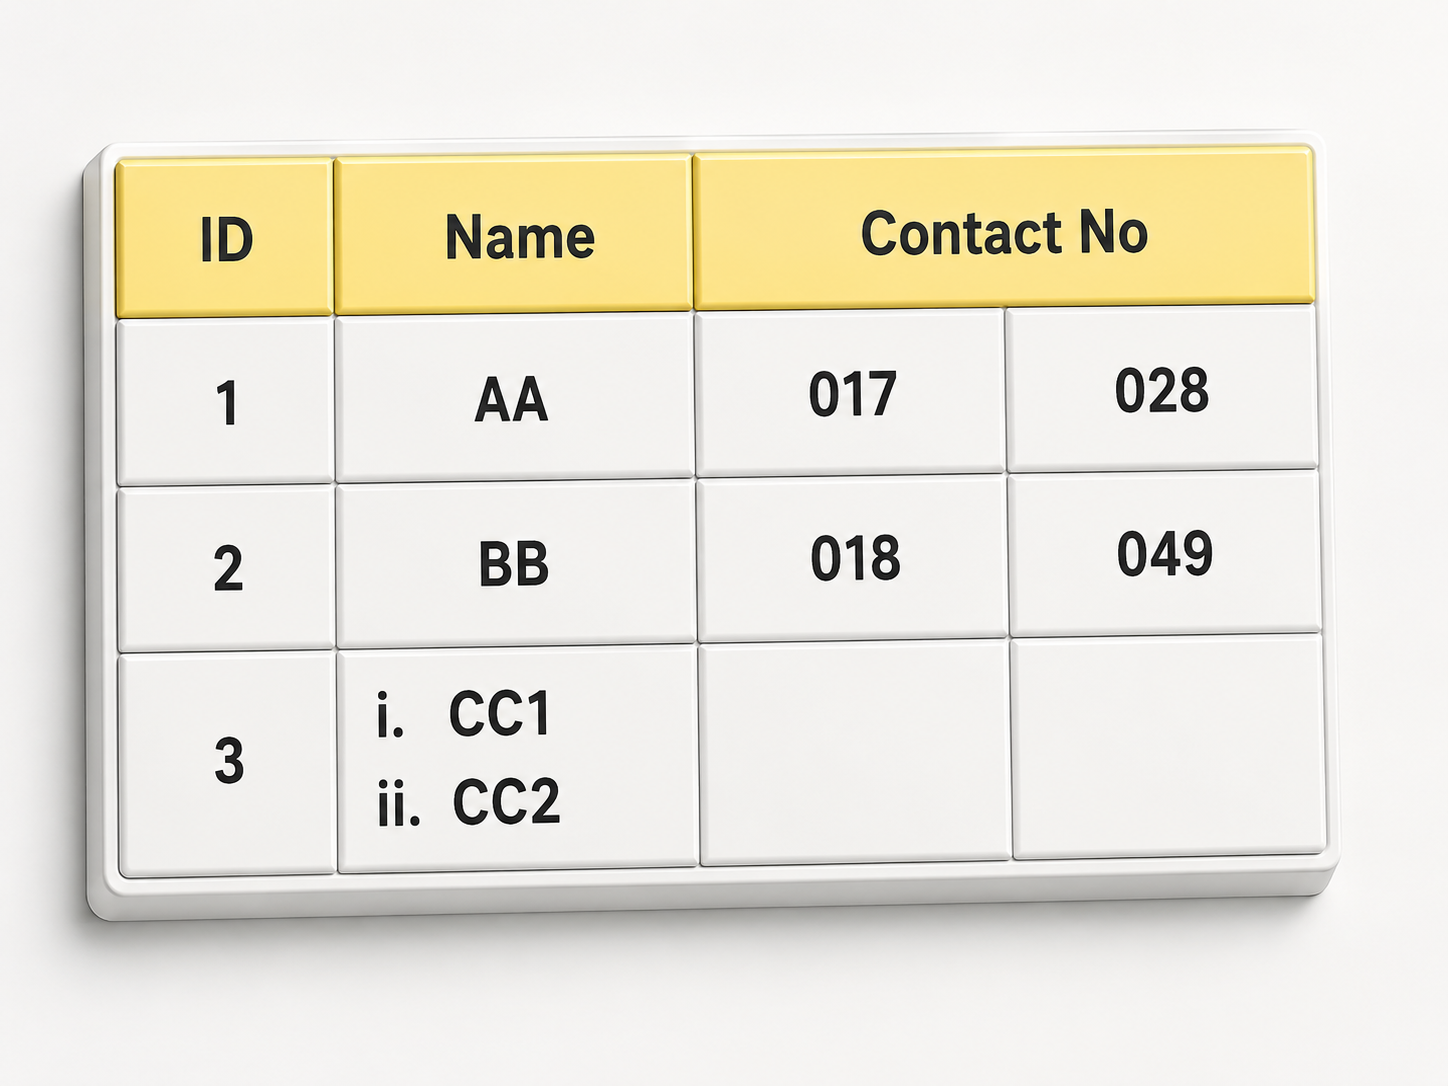
\includegraphics[width=0.95\linewidth,height=0.11\textheight,keepaspectratio]{chapters/Chapter04/topics/images/ex23_3d_contact_no_colspan.png}
}{
\fbox{\parbox{0.90\linewidth}{\centering\vspace{0.45cm}
\textbf{চিত্র}\\[3pt]
File: \texttt{chapters/Chapter04/topics/images/ex23\_3d\_contact\_no\_colspan.png}
\vspace{0.45cm}}}
}
\captionof{figure}{Contact No table with bgcolor and colspan}
\end{center}

\begin{keypointbox}{চিত্র ব্যাখ্যা}
Contact No heading দুই column জুড়ে আছে। Header row-তে yellow background color ব্যবহার করা হয়েছে। শেষ row-তে ordered list type i ব্যবহার করা হয়েছে।
\end{keypointbox}

\par\noindent{\color{purple!70!black}\bfseries\small কোড}\par\vspace{-4pt}
\begin{verbatim}
<!DOCTYPE html>
<html>
<head>
  <title>HTML Table Example</title>
</head>
<body>
<table border="1" cellspacing="0">
<tr bgcolor="yellow">
  <th>ID</th>
  <th>Name</th>
  <th colspan="2">Contact No</th>
</tr>
<tr>
  <td>1</td>
  <td>AA</td>
  <td>017</td>
  <td>028</td>
</tr>
<tr>
  <td>2</td>
  <td>BB</td>
  <td>018</td>
  <td>049</td>
</tr>
<tr>
  <td>3</td>
  <td>
    <ol type="i">
      <li>CC1</li>
      <li>CC2</li>
    </ol>
  </td>
  <td colspan="2"><br></td>
</tr>
</table>
</body>
</html>
\end{verbatim}
\vspace{-6pt}

\subsubsection{Exercise 24: Govt. Rajendra College Table with Image and Links}

\begin{center}
\IfFileExists{chapters/Chapter04/topics/images/ex24_3d_college_image_links.png}{
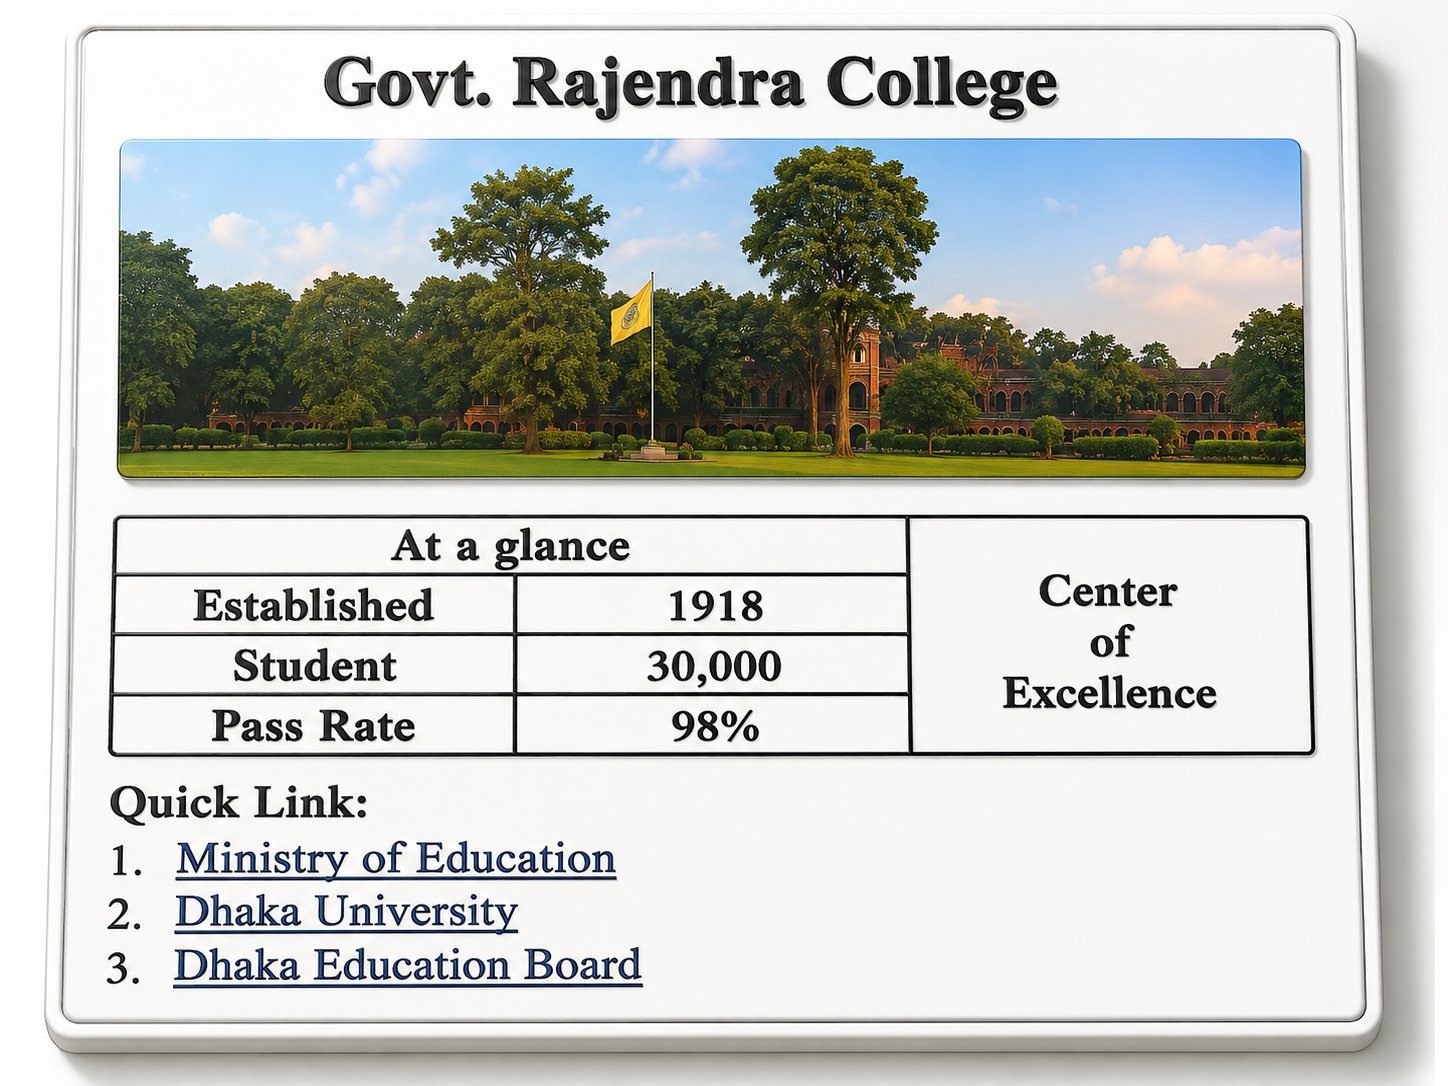
\includegraphics[width=0.95\linewidth,height=0.11\textheight,keepaspectratio]{chapters/Chapter04/topics/images/ex24_3d_college_image_links.png}
}{
\fbox{\parbox{0.90\linewidth}{\centering\vspace{0.45cm}
\textbf{চিত্র}\\[3pt]
File: \texttt{chapters/Chapter04/topics/images/ex24\_3d\_college\_image\_links.png}
\vspace{0.45cm}}}
}
\captionof{figure}{Govt. Rajendra College table with image, nested info and quick links}
\end{center}

\begin{keypointbox}{চিত্র ব্যাখ্যা}
এই example-এ heading, image, At a glance table এবং quick link একসাথে ব্যবহার করা হয়েছে। Center of Excellence cell চার row জুড়ে আছে।
\end{keypointbox}

\begin{keypointbox}{চিত্র দেখে code লেখার ধাপ}
প্রথমে figure-এর total row ও column গুনবে। এরপর কোন cell একাধিক column জুড়ে আছে তা দেখে \texttt{colspan} এবং কোন cell একাধিক row জুড়ে আছে তা দেখে \texttt{rowspan} বসাবে। তারপর image, link, list বা nested table থাকলে সংশ্লিষ্ট tag cell-এর ভিতরে লিখবে।
\end{keypointbox}

\par\noindent{\color{purple!70!black}\bfseries\small কোড}\par\vspace{-4pt}
\begin{verbatim}
<!DOCTYPE html>
<html>
<head>
  <title>HTML Table Example</title>
</head>
<body>
<h3 align="center">Govt. Rajendra College</h3>
<img src="college.jpg" width="400" height="200" align="center"><br>
<table border="1" cellspacing="0" align="center">
<tr>
  <th colspan="2">At a glance</th>
  <td rowspan="4" align="center">Center<br>of<br>Excellence</td>
</tr>
<tr>
  <th>Established</th>
  <td>1918</td>
</tr>
<tr>
  <th>Student</th>
  <td>30,000</td>
</tr>
<tr>
  <th>Pass Rate</th>
  <td>98%</td>
</tr>
</table>
<p>Quick Link:<br>
<a href="http://www.moedu.gov.bd">Ministry of Education</a><br>
<a href="www.du.ac.bd">Dhaka University</a><br>
<a href="www.dhakaeducationboard.gov.bd">Dhaka Education Board</a><br>
</p>
</body>
</html>
\end{verbatim}
\vspace{-6pt}

\subsubsection{Exercise 25: Department Male/Female Table with Photo}

\begin{center}
\IfFileExists{chapters/Chapter04/topics/images/ex25_3d_department_photo.png}{
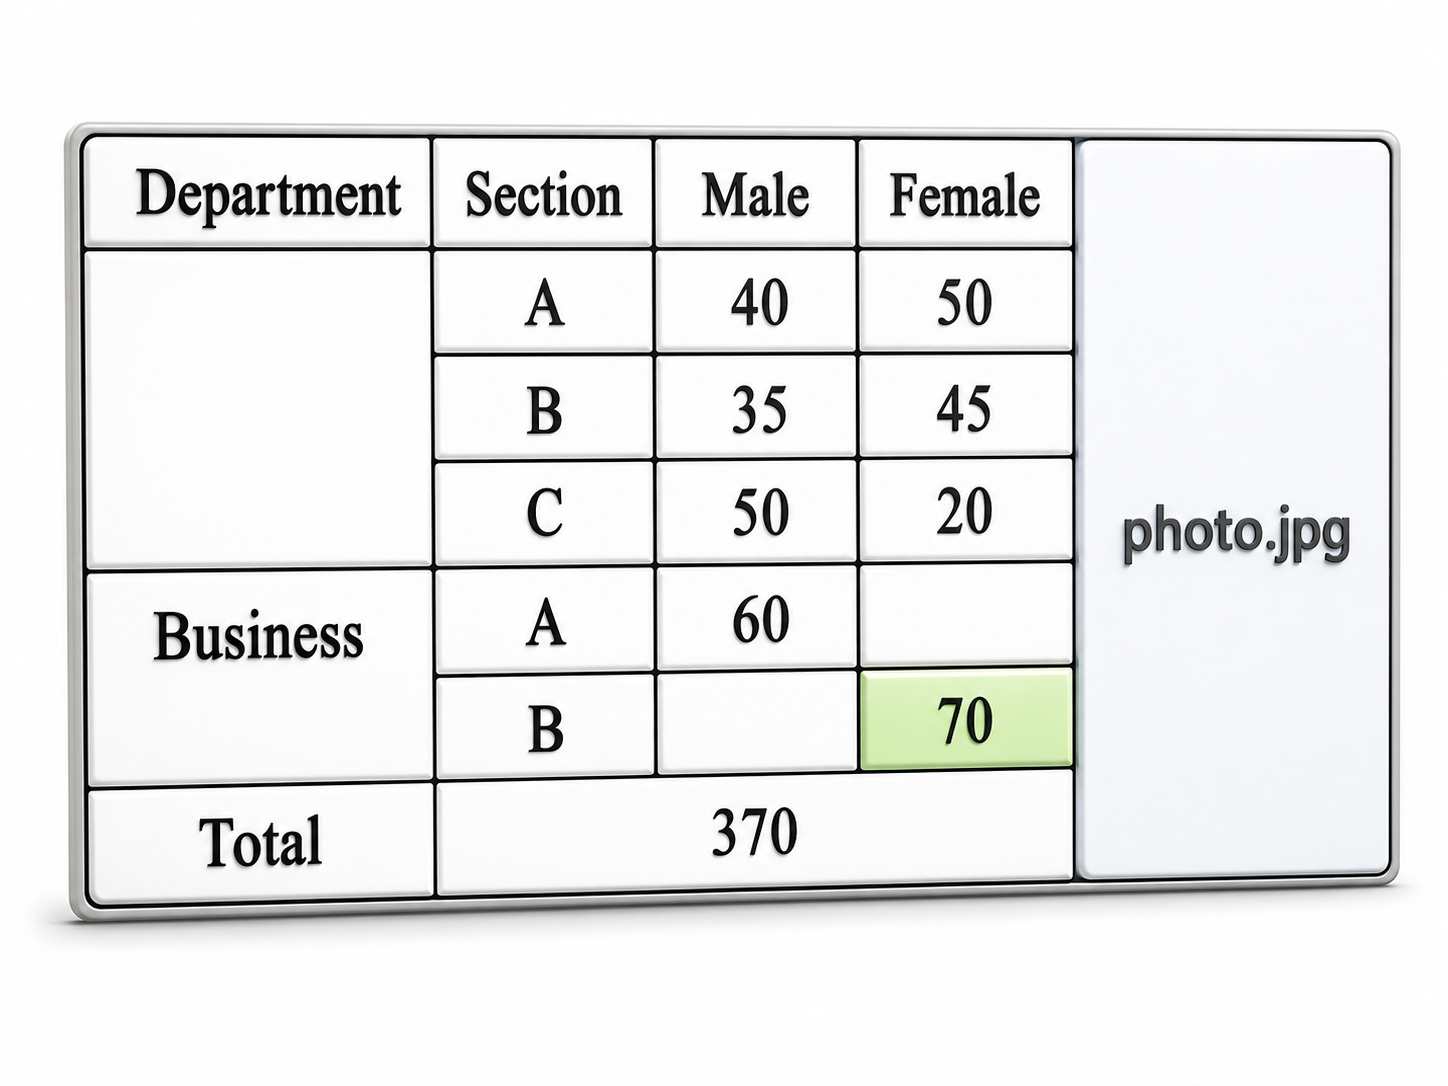
\includegraphics[width=0.95\linewidth,height=0.11\textheight,keepaspectratio]{chapters/Chapter04/topics/images/ex25_3d_department_photo.png}
}{
\fbox{\parbox{0.90\linewidth}{\centering\vspace{0.45cm}
\textbf{চিত্র}\\[3pt]
File: \texttt{chapters/Chapter04/topics/images/ex25\_3d\_department\_photo.png}
\vspace{0.45cm}}}
}
\captionof{figure}{Department table with photo, rowspan, total and green cell}
\end{center}

\begin{keypointbox}{চিত্র ব্যাখ্যা}
Photo column সাত row জুড়ে আছে। Business cell দুই row জুড়ে আছে। 70 cell-এর background green। Total row-তে total text ও 370 value center aligned করে দেখানো হয়েছে।
\end{keypointbox}

\par\noindent{\color{purple!70!black}\bfseries\small কোড}\par\vspace{-4pt}
\begin{verbatim}
<!DOCTYPE html>
<html>
<head>
  <title>HTML Table Example</title>
</head>
<body>
  <table border="1" cellspacing="0">
    <tr>
      <th>Department</th><th>Section</th><th>Male</th><th>Female</th>
      <th rowspan="7"><img src="photo.jpg" width="60" height="50" alt="Photo"></th>
    </tr>
    <tr><td rowspan="3">&nbsp;</td><td>A</td><td>40</td><td>50</td></tr>
    <tr><td>B</td><td>35</td><td>45</td></tr>
    <tr><td>C</td><td>50</td><td>20</td></tr>
    <tr><td rowspan="2" align="center">Business</td><td>A</td><td>60</td><td>&nbsp;</td></tr>
    <tr><td>B</td><td>&nbsp;</td><td bgcolor="green">70</td></tr>
    <tr><td align="center">Total</td><td colspan="3" align="center">370</td></tr>
  </table>
</body>
</html>
\end{verbatim}
\vspace{-6pt}

\Needspace{10\baselineskip}
\subsubsection{Exercise 26: Science, Commerce and Humanities Table}

\begin{boardbox}{Concept}
Group-wise subject table-এ first column group দেখায় এবং বাকি columnগুলো subject list দেখায়। চিত্র দেখে row ও column count ঠিক করা সবচেয়ে জরুরি।
\end{boardbox}

\begin{center}
\IfFileExists{chapters/Chapter04/topics/images/ex26_3d_group_subjects.png}{
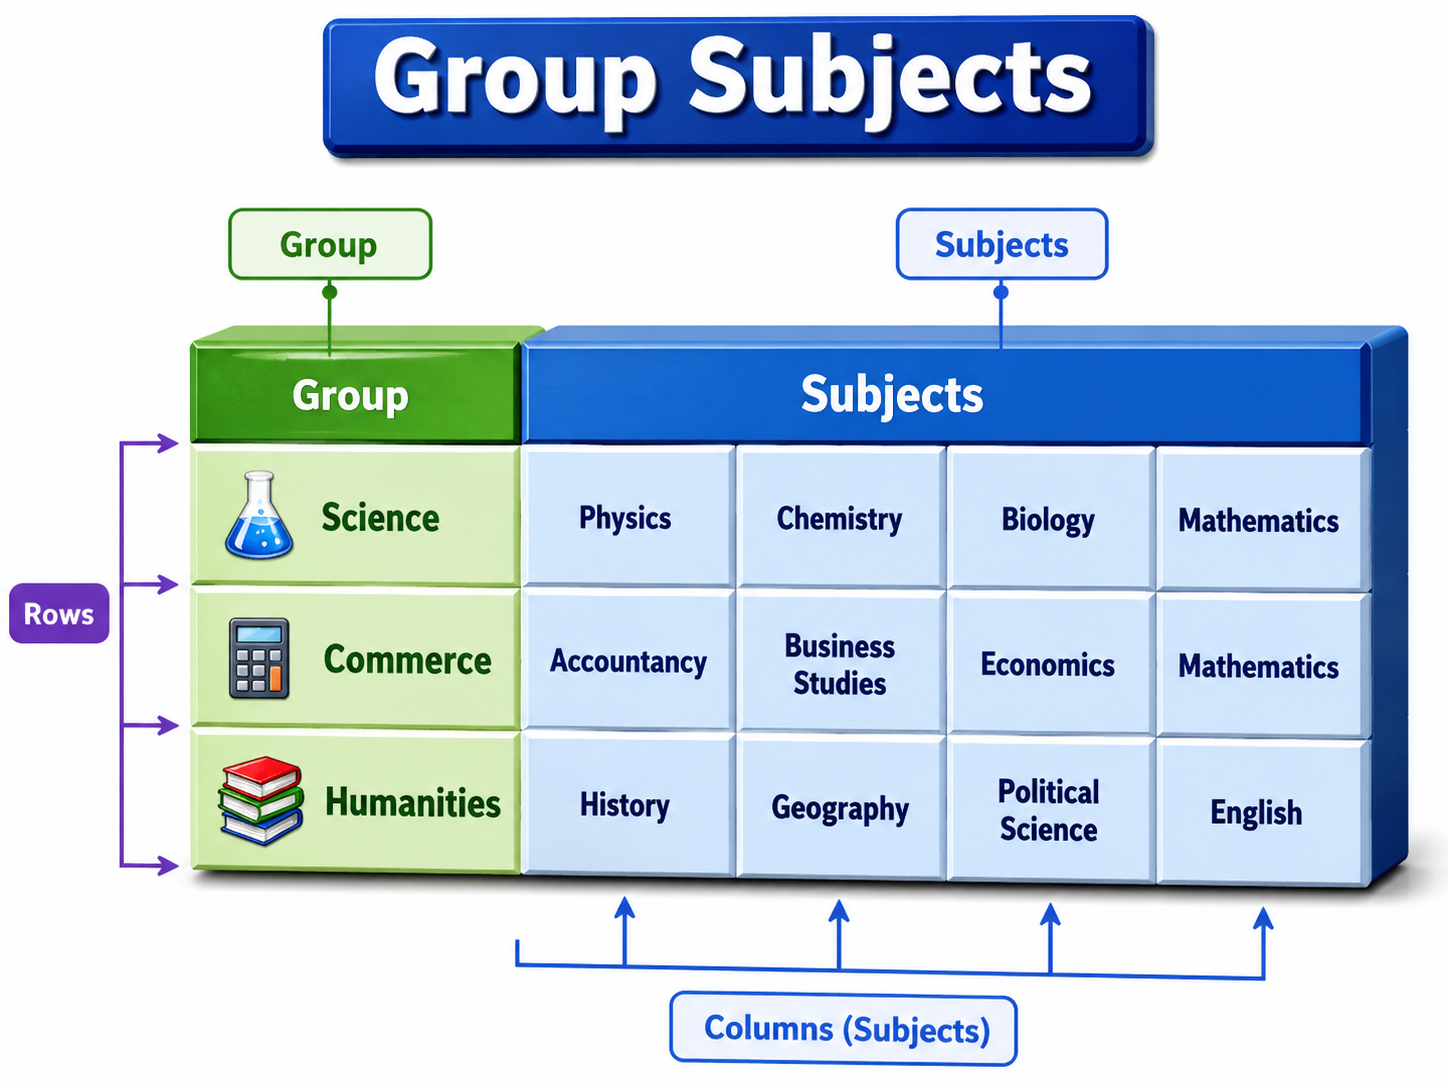
\includegraphics[width=0.95\linewidth,height=0.11\textheight,keepaspectratio]{chapters/Chapter04/topics/images/ex26_3d_group_subjects.png}
}{
\fbox{\parbox{0.90\linewidth}{\centering\vspace{0.4cm}
\textbf{চিত্র}\\
File: \texttt{chapters/Chapter04/topics/images/ex26\_3d\_group\_subjects.png}
\vspace{0.4cm}}}
}
\captionof{figure}{Exercise 26-এর subject group চিত্র}
\end{center}

\begin{keypointbox}{চিত্র ব্যাখ্যা}
চিত্রে Group Subjects নামে একটি table আছে। প্রথম column-এ Science, Commerce ও Humanities group দেখানো হয়েছে। প্রতিটি group row-তে Physics/Chemistry/Biology/Mathematics, Accountancy/Business Studies/Economics/Mathematics এবং History/Geography/Political Science/English subject দেওয়া আছে।
\end{keypointbox}

\begin{keypointbox}{চিত্র দেখে code লেখার ধাপ}
প্রথমে title row-তে \texttt{colspan="5"} ব্যবহার করবে, কারণ table-এ Group সহ মোট 5টি column আছে। দ্বিতীয় row-তে Group ও Subjects heading লিখবে; Subjects heading চারটি subject column জুড়ে থাকবে। এরপর তিনটি group row লিখবে।
\end{keypointbox}

\par\noindent{\color{purple!70!black}\bfseries\small কোড}\par\vspace{-4pt}
\begin{verbatim}
<!DOCTYPE html>
<html>
<head>
  <title>HTML Table Example</title>
</head>
<body>
<table border="1" cellspacing="0" cellpadding="6" align="center">
  <tr>
    <th colspan="5">Group Subjects</th>
  </tr>
  <tr>
    <th>Group</th>
    <th colspan="4">Subjects</th>
  </tr>
  <tr>
    <td>Science</td>
    <td>Physics</td>
    <td>Chemistry</td>
    <td>Biology</td>
    <td>Mathematics</td>
  </tr>
  <tr>
    <td>Commerce</td>
    <td>Accountancy</td>
    <td>Business Studies</td>
    <td>Economics</td>
    <td>Mathematics</td>
  </tr>
  <tr>
    <td>Humanities</td>
    <td>History</td>
    <td>Geography</td>
    <td>Political Science</td>
    <td>English</td>
  </tr>
</table>
</body>
</html>
\end{verbatim}
\vspace{-6pt}
\subsubsection{Exercise 27: List Inside Table Cell}

\begin{center}
\IfFileExists{chapters/Chapter04/topics/images/ex27_3d_lists_inside_table.png}{
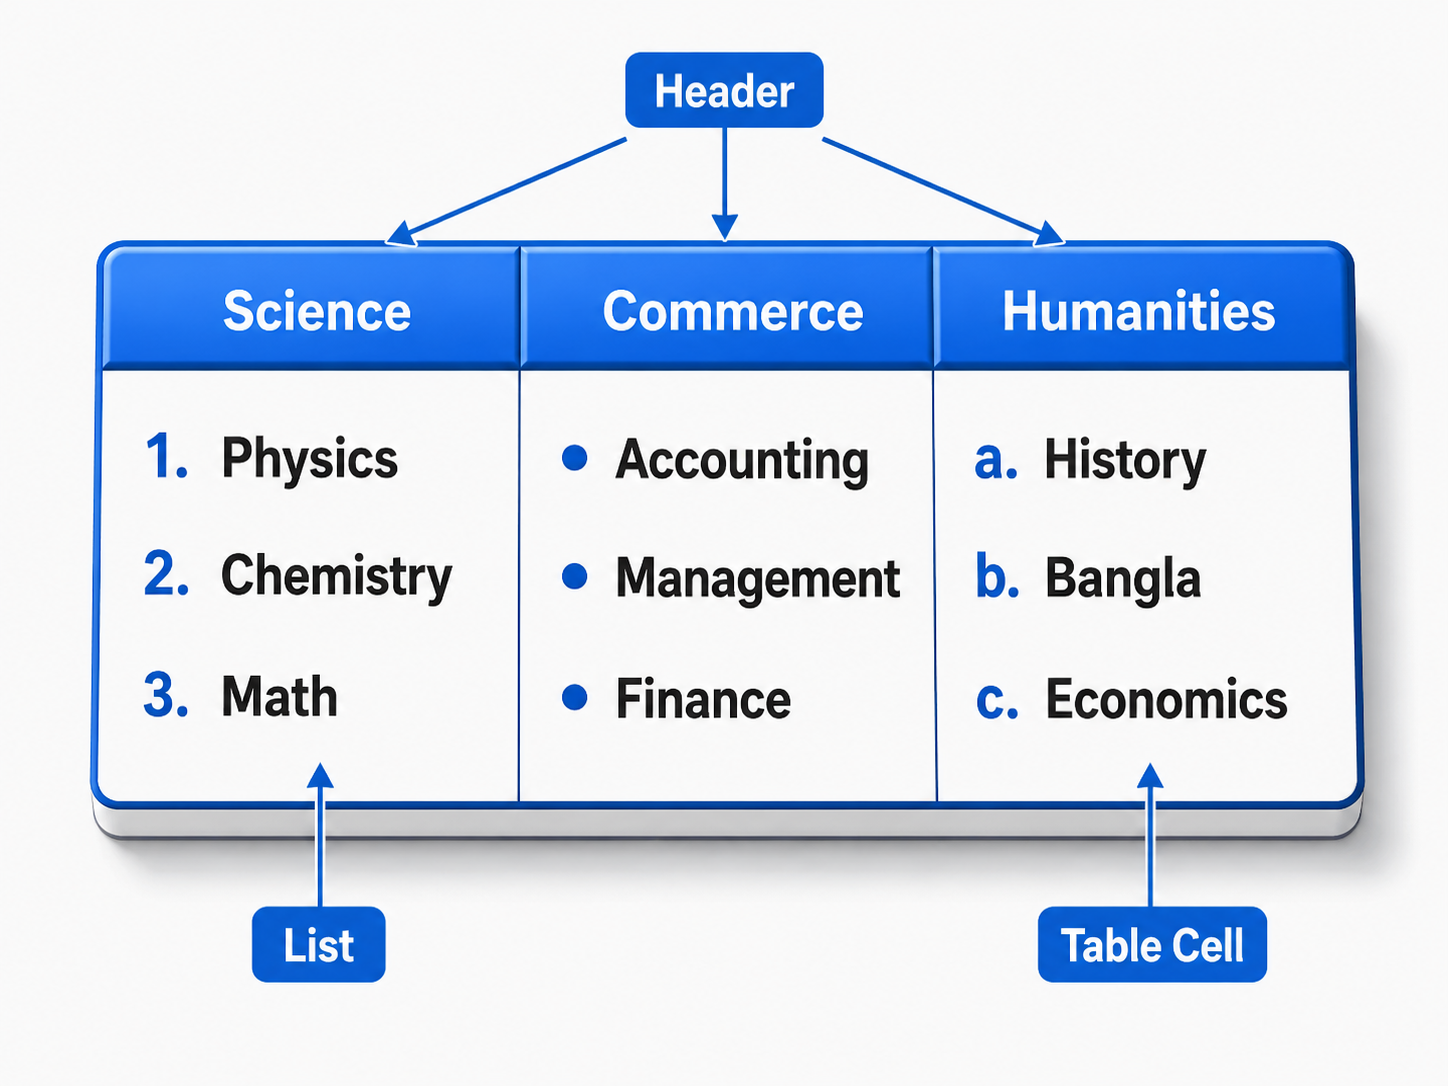
\includegraphics[width=0.95\linewidth,height=0.11\textheight,keepaspectratio]{chapters/Chapter04/topics/images/ex27_3d_lists_inside_table.png}
}{
\fbox{\parbox{0.90\linewidth}{\centering\vspace{0.45cm}
\textbf{চিত্র}\\[3pt]
File: \texttt{chapters/Chapter04/topics/images/ex27\_3d\_lists\_inside\_table.png}
\vspace{0.45cm}}}
}
\captionof{figure}{List inside table cell: Science, Commerce ও Humanities}
\end{center}

\begin{keypointbox}{চিত্র ব্যাখ্যা}
এই table-এ তিনটি column আছে: Science, Commerce ও Humanities। প্রতিটি cell-এর ভিতরে আলাদা type-এর list ব্যবহার করা হয়েছে: ordered list, unordered list এবং alphabetic ordered list।
\end{keypointbox}

\begin{keypointbox}{চিত্র দেখে code লেখার ধাপ}
প্রথমে figure-এর total row ও column গুনবে। এরপর কোন cell একাধিক column জুড়ে আছে তা দেখে \texttt{colspan} এবং কোন cell একাধিক row জুড়ে আছে তা দেখে \texttt{rowspan} বসাবে। তারপর image, link, list বা nested table থাকলে সংশ্লিষ্ট tag cell-এর ভিতরে লিখবে।
\end{keypointbox}

\par\noindent{\color{purple!70!black}\bfseries\small কোড}\par\vspace{-4pt}
\begin{verbatim}
<!DOCTYPE html>
<html>
<head>
  <title>HTML Table Example</title>
</head>
<body>
<table border="1" cellspacing="0">
<tr>
  <th>Science</th>
  <th>Commerce</th>
  <th>Humanities</th>
</tr>
<tr>
  <td><ol><li>Physics</li><li>Chemistry</li><li>Math</li></ol></td>
  <td><ul><li>Accounting</li><li>Management</li><li>Finance</li></ul></td>
  <td><ol type="a"><li>History</li><li>Bangla</li><li>Economics</li></ol></td>
</tr>
</table>
</body>
</html>
\end{verbatim}
\vspace{-6pt}

\subsubsection{Exercise 28: Teacher Information Table with Picture}

\begin{center}
\IfFileExists{chapters/Chapter04/topics/images/ex28_3d_teacher_info_picture.png}{
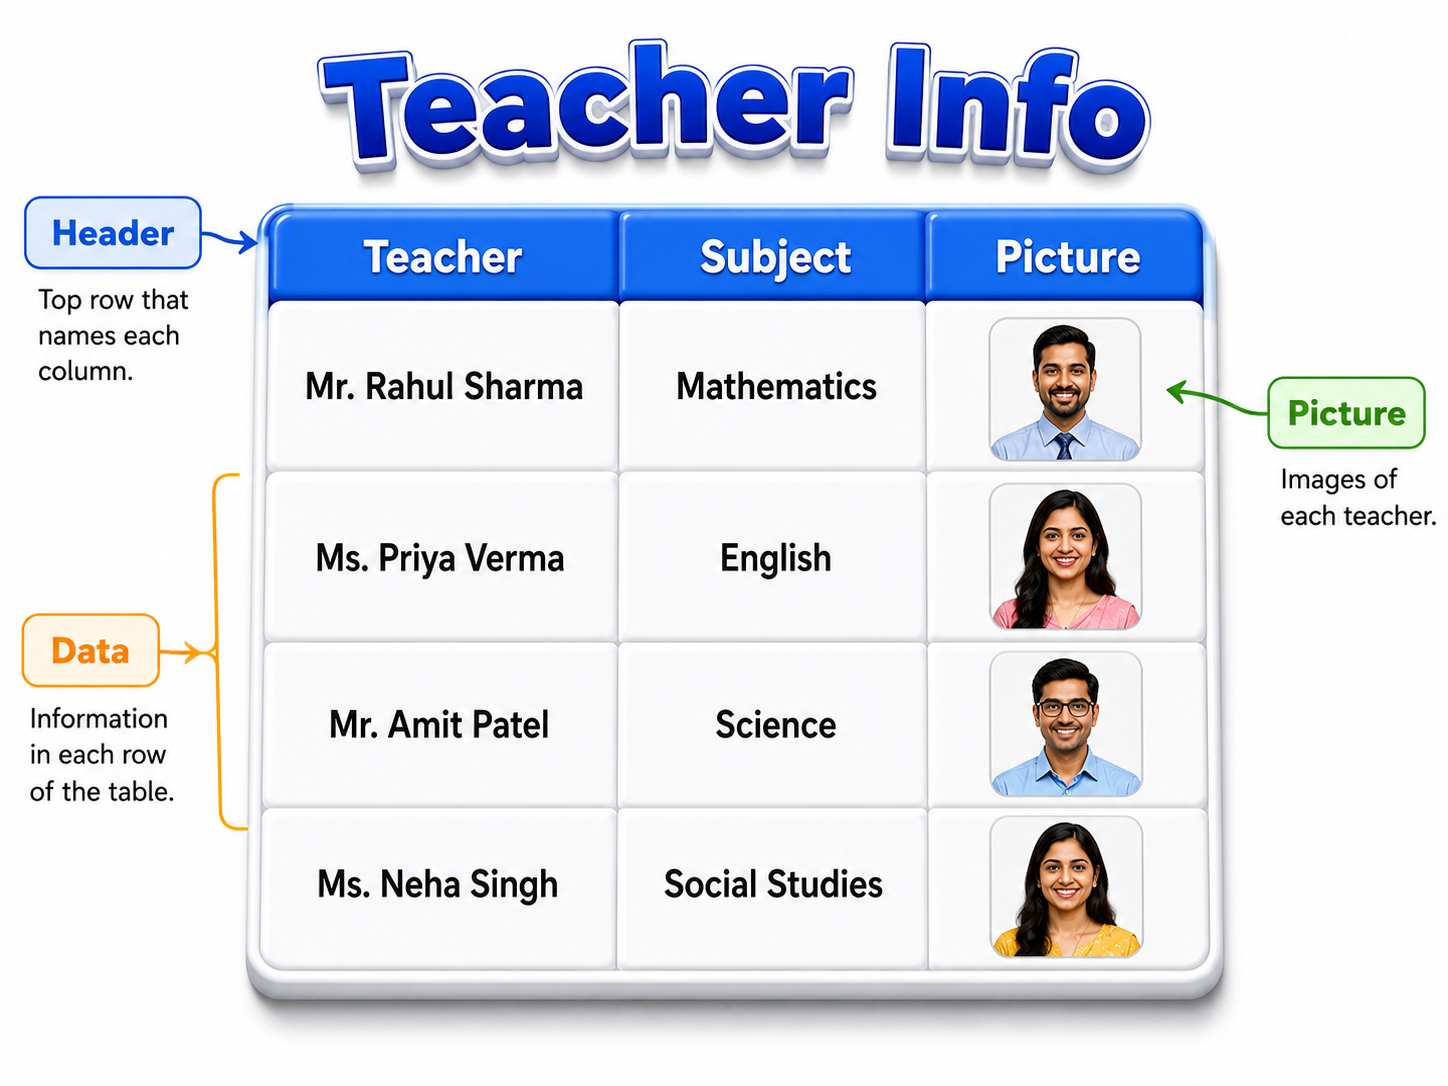
\includegraphics[width=0.95\linewidth,height=0.11\textheight,keepaspectratio]{chapters/Chapter04/topics/images/ex28_3d_teacher_info_picture.png}
}{
\fbox{\parbox{0.90\linewidth}{\centering\vspace{0.45cm}
\textbf{চিত্র}\\[3pt]
File: \texttt{chapters/Chapter04/topics/images/ex28\_3d\_teacher\_info\_picture.png}
\vspace{0.45cm}}}
}
\captionof{figure}{Teacher Info table with subject and picture column}
\end{center}

\begin{keypointbox}{চিত্র ব্যাখ্যা}
চিত্রে Teacher Info heading আছে এবং table-এ Teacher, Subject ও Picture--এই তিনটি column দেখা যায়। প্রতিটি row-তে teacher name, subject এবং সংশ্লিষ্ট picture রাখা হয়েছে।
\end{keypointbox}

\begin{keypointbox}{চিত্র দেখে code লেখার ধাপ}
প্রথমে title/heading আলাদা করবে। তারপর তিনটি column--Teacher, Subject, Picture--লিখবে। Picture column-এর প্রতিটি cell-এ \texttt{<img>} tag বসাবে এবং image size নির্ধারণ করবে।
\end{keypointbox}

\par\noindent{\color{purple!70!black}\bfseries\small কোড}\par\vspace{-4pt}
\begin{verbatim}
<!DOCTYPE html>
<html>
<head>
  <title>HTML Table Example</title>
</head>
<body>
<h2 align="center">Teacher Info</h2>
<table border="1" align="center" cellspacing="0" cellpadding="6">
<tr>
  <th>Teacher</th>
  <th>Subject</th>
  <th>Picture</th>
</tr>
<tr>
  <td>Mr. Rahul Sharma</td>
  <td>Mathematics</td>
  <td><img src="rahul.jpg" width="55" height="60" alt="Rahul Sharma"></td>
</tr>
<tr>
  <td>Mrs. Priya Verma</td>
  <td>English</td>
  <td><img src="priya.jpg" width="55" height="60" alt="Priya Verma"></td>
</tr>
<tr>
  <td>Mr. Amit Patel</td>
  <td>Science</td>
  <td><img src="amit.jpg" width="55" height="60" alt="Amit Patel"></td>
</tr>
<tr>
  <td>Ms. Neha Singh</td>
  <td>Social Studies</td>
  <td><img src="neha.jpg" width="55" height="60" alt="Neha Singh"></td>
</tr>
</table>
</body>
</html>
\end{verbatim}
\vspace{-6pt}

\subsubsection{Exercise 29: Bangladesh Places Table with Photo}

\begin{center}
\IfFileExists{chapters/Chapter04/topics/images/ex29_3d_bangladesh_places.png}{
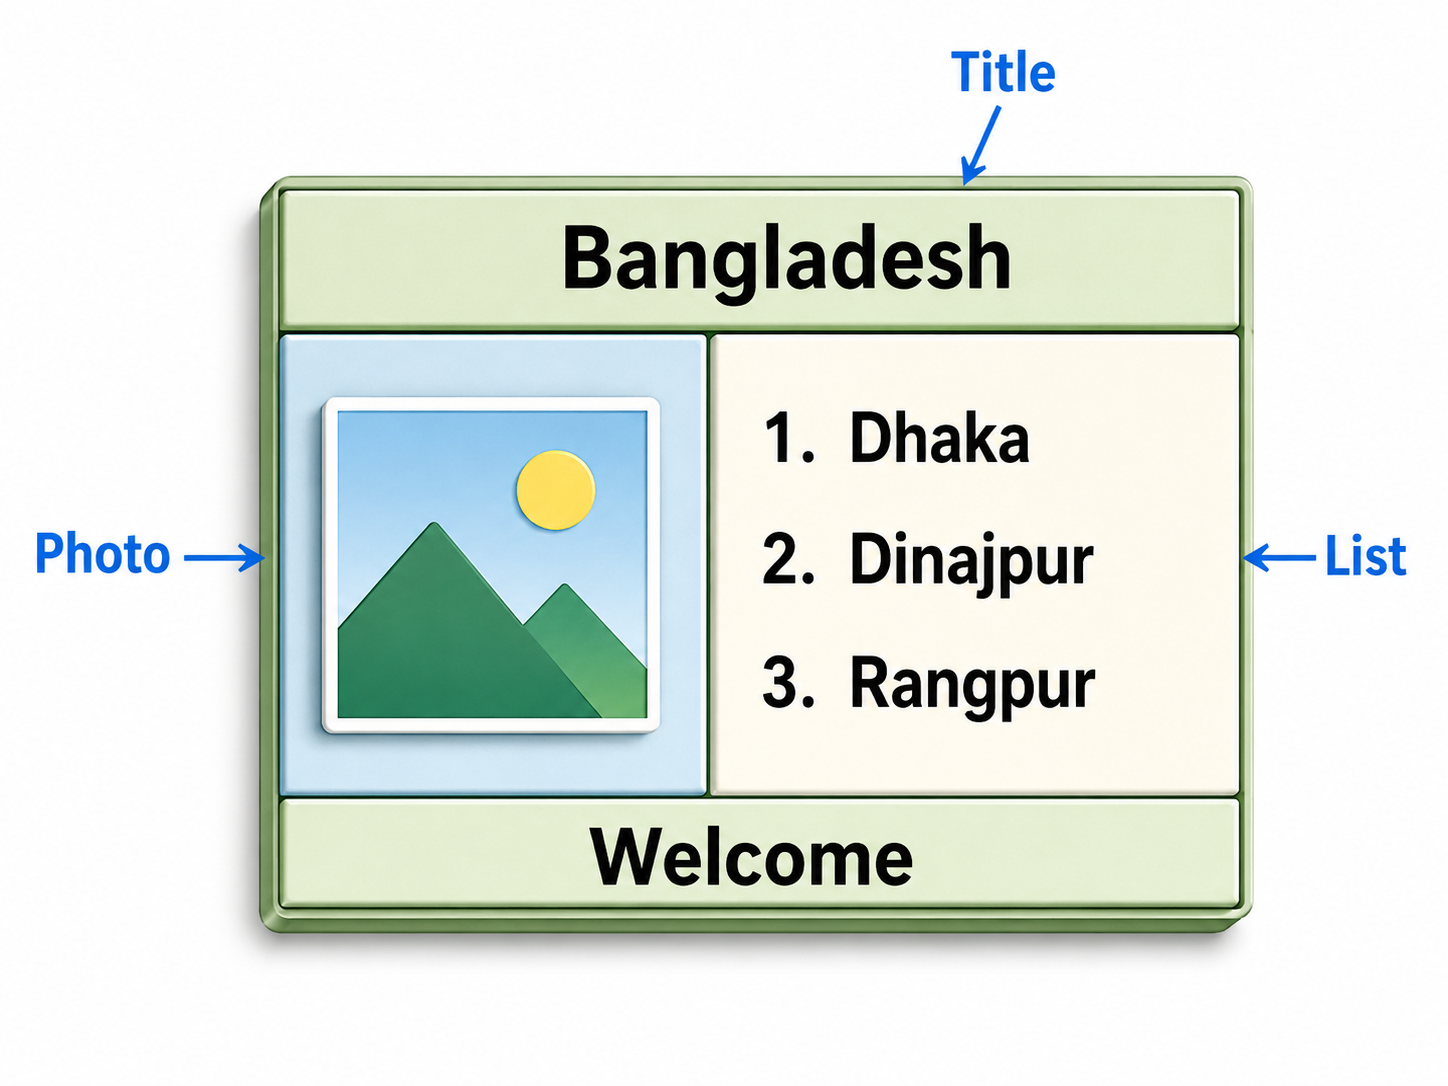
\includegraphics[width=0.95\linewidth,height=0.11\textheight,keepaspectratio]{chapters/Chapter04/topics/images/ex29_3d_bangladesh_places.png}
}{
\fbox{\parbox{0.90\linewidth}{\centering\vspace{0.45cm}
\textbf{চিত্র}\\[3pt]
File: \texttt{chapters/Chapter04/topics/images/ex29\_3d\_bangladesh\_places.png}
\vspace{0.45cm}}}
}
\captionof{figure}{Bangladesh table with photo and ordered list}
\end{center}

\begin{keypointbox}{চিত্র ব্যাখ্যা}
এই table-এ top heading এবং bottom welcome row দুটি column জুড়ে আছে। মাঝের row-তে বাম cell-এ image এবং ডান cell-এ ordered list রাখা হয়েছে।
\end{keypointbox}

\begin{keypointbox}{চিত্র দেখে code লেখার ধাপ}
প্রথমে figure-এর total row ও column গুনবে। এরপর কোন cell একাধিক column জুড়ে আছে তা দেখে \texttt{colspan} এবং কোন cell একাধিক row জুড়ে আছে তা দেখে \texttt{rowspan} বসাবে। তারপর image, link, list বা nested table থাকলে সংশ্লিষ্ট tag cell-এর ভিতরে লিখবে।
\end{keypointbox}

\par\noindent{\color{purple!70!black}\bfseries\small কোড}\par\vspace{-4pt}
\begin{verbatim}
<!DOCTYPE html>
<html>
<head>
  <title>HTML Table Example</title>
</head>
<body>
<table border="1" cellspacing="0">
<tr><th colspan="2">Bangladesh</th></tr>
<tr>
  <td><img src="photo.jpg" width="60" height="50" align="center"><br>Photo</td>
  <td>
    <ol>
      <li>Dhaka</li>
      <li>Dinajpur</li>
      <li>Rangpur</li>
    </ol>
  </td>
</tr>
<tr><th colspan="2">Welcome</th></tr>
</table>
</body>
</html>
\end{verbatim}
\vspace{-6pt}

\subsubsection{Exercise 30: Choose Your Site Table with Links}

\begin{center}
\IfFileExists{chapters/Chapter04/topics/images/ex30_3d_choose_site_links.png}{
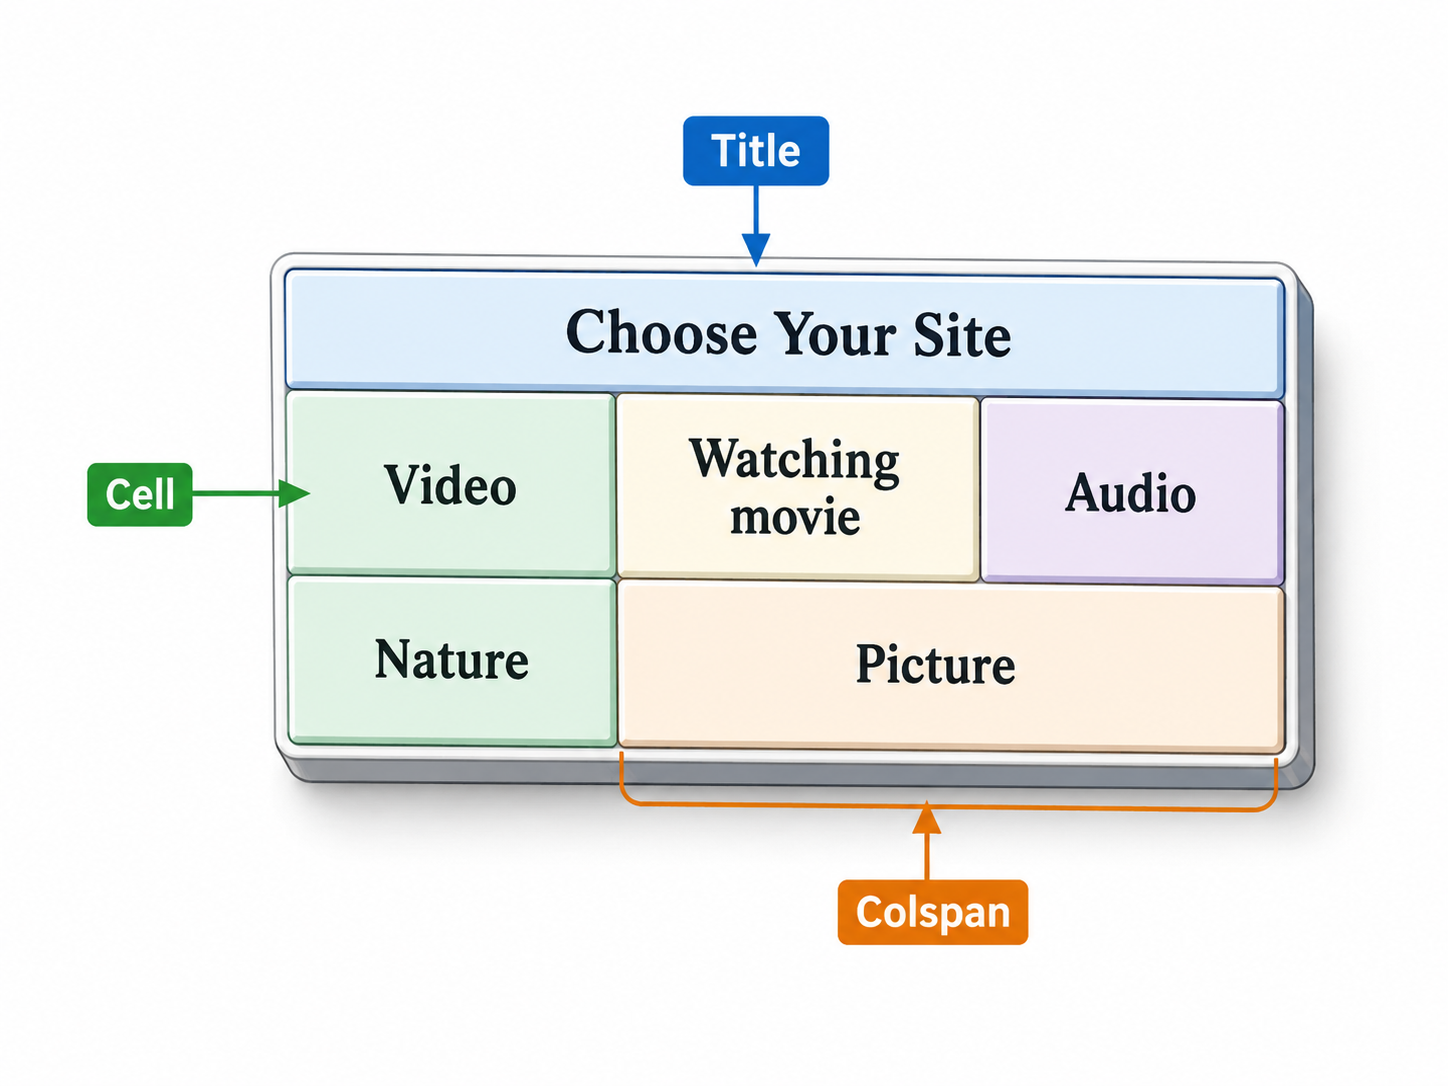
\includegraphics[width=0.95\linewidth,height=0.11\textheight,keepaspectratio]{chapters/Chapter04/topics/images/ex30_3d_choose_site_links.png}
}{
\fbox{\parbox{0.90\linewidth}{\centering\vspace{0.45cm}
\textbf{চিত্র}\\[3pt]
File: \texttt{chapters/Chapter04/topics/images/ex30\_3d\_choose\_site\_links.png}
\vspace{0.45cm}}}
}
\captionof{figure}{Choose Your Site table with centered and underlined text}
\end{center}

\begin{keypointbox}{চিত্র ব্যাখ্যা}
এখানে \texttt{colspan="3"} দিয়ে title row তিনটি column জুড়ে আছে। Video ও Nature underline করা হয়েছে এবং Picture cell দুই column জুড়ে আছে।
\end{keypointbox}

\par\noindent{\color{purple!70!black}\bfseries\small কোড}\par\vspace{-4pt}
\begin{verbatim}
<!DOCTYPE html>
<html>
<head>
  <title>HTML Table Example</title>
</head>
<body>
<table border="1" cellspacing="0">
<tr>
  <th colspan="3">Choose Your Site</th>
</tr>
<tr>
  <td align="center"><u>Video</u><br></td>
  <td>Watching<br><p align="center">movie</p></td>
  <td>Audio</td>
</tr>
<tr>
  <td align="center"><u>Nature</u></td>
  <td colspan="2" align="center"><br>Picture</td>
</tr>
</table>
</body>
</html>
\end{verbatim}
\vspace{-6pt}

\subsubsection{Exercise 31: XY Showroom Table}

\begin{center}
\IfFileExists{chapters/Chapter04/topics/images/ex31_3d_xy_showroom.png}{
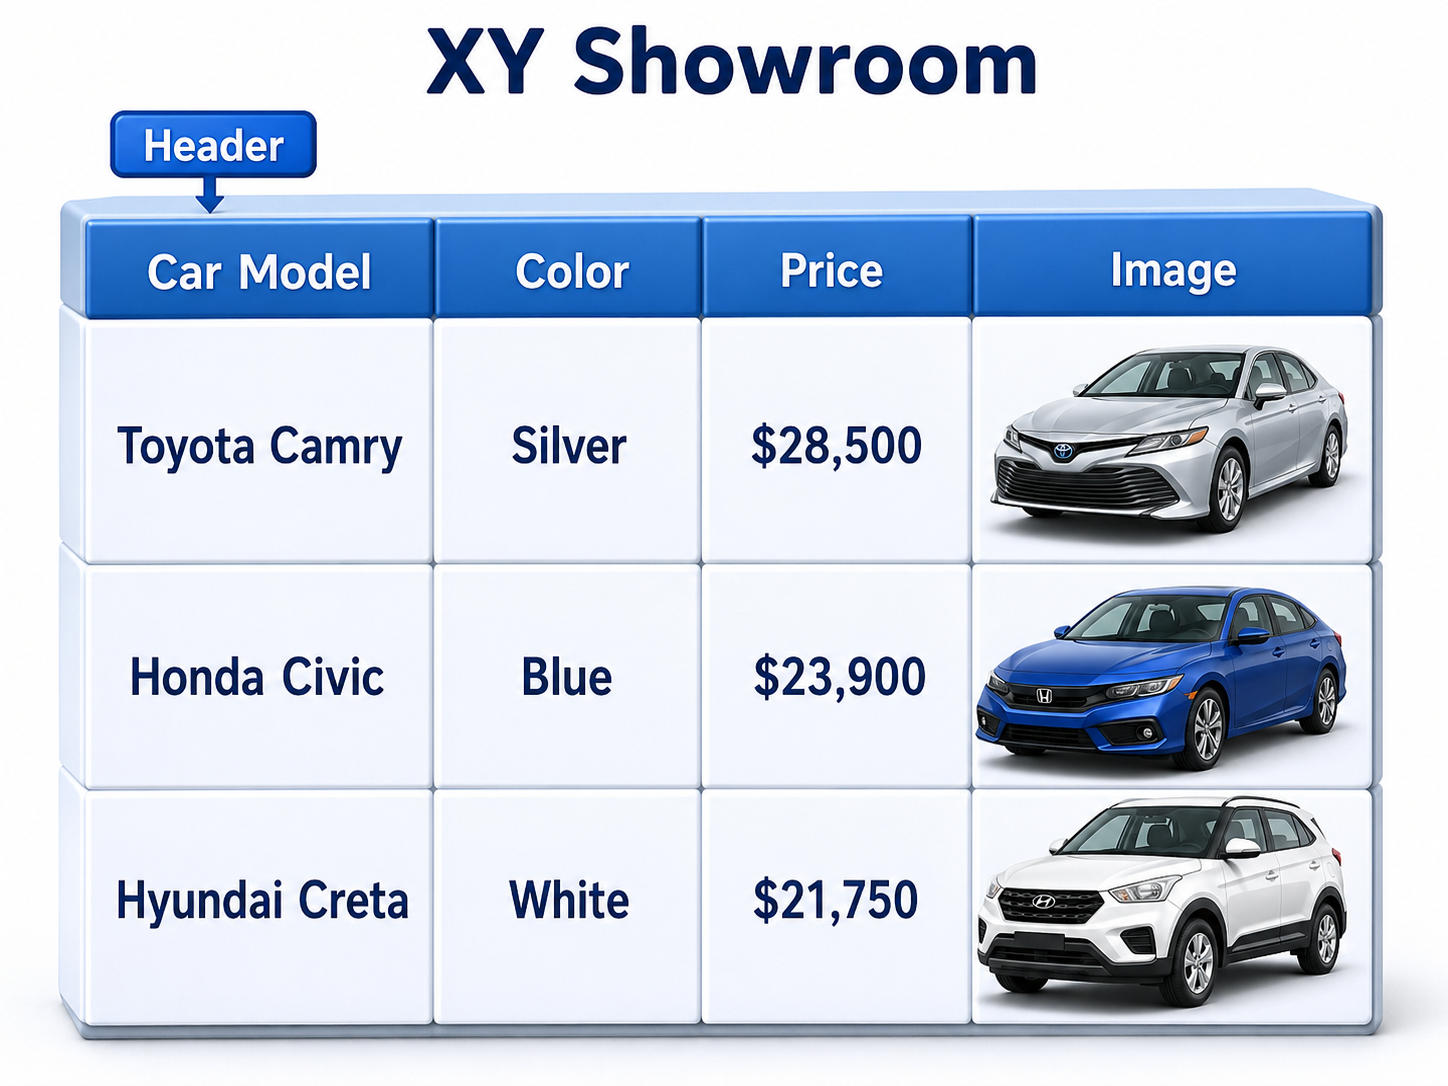
\includegraphics[width=0.95\linewidth,height=0.11\textheight,keepaspectratio]{chapters/Chapter04/topics/images/ex31_3d_xy_showroom.png}
}{
\fbox{\parbox{0.90\linewidth}{\centering\vspace{0.45cm}
\textbf{চিত্র}\\[3pt]
File: \texttt{chapters/Chapter04/topics/images/ex31\_3d\_xy\_showroom.png}
\vspace{0.45cm}}}
}
\captionof{figure}{XY Showroom table with car model, color, price and image}
\end{center}

\begin{keypointbox}{চিত্র ব্যাখ্যা}
চিত্রে XY Showroom heading-এর নিচে Car Model, Color, Price এবং Image--চারটি column আছে। প্রতিটি car row-তে model, color, price এবং car image দেখানো হয়েছে।
\end{keypointbox}

\begin{keypointbox}{চিত্র দেখে code লেখার ধাপ}
প্রথমে table-এর উপরে \texttt{<h2>} heading লিখবে। তারপর চারটি header cell তৈরি করবে। প্রতিটি row-তে car model, color, price এবং image cell লিখবে। Image column-এ \texttt{<img>} tag ব্যবহার করবে।
\end{keypointbox}

\par\noindent{\color{purple!70!black}\bfseries\small কোড}\par\vspace{-4pt}
\begin{verbatim}
<!DOCTYPE html>
<html>
<head>
  <title>XY Showroom</title>
</head>
<body>
<h2 align="center">XY Showroom</h2>
<table border="1" align="center" cellspacing="0" cellpadding="6">
<tr>
  <th>Car Model</th>
  <th>Color</th>
  <th>Price</th>
  <th>Image</th>
</tr>
<tr>
  <td>Toyota Camry</td>
  <td>Silver</td>
  <td>$28,500</td>
  <td><img src="camry.jpg" width="100" height="60" alt="Toyota Camry"></td>
</tr>
<tr>
  <td>Honda Civic</td>
  <td>Blue</td>
  <td>$23,900</td>
  <td><img src="civic.jpg" width="100" height="60" alt="Honda Civic"></td>
</tr>
<tr>
  <td>Hyundai Creta</td>
  <td>White</td>
  <td>$21,750</td>
  <td><img src="creta.jpg" width="100" height="60" alt="Hyundai Creta"></td>
</tr>
</table>
</body>
</html>
\end{verbatim}
\vspace{-6pt}

\subsubsection{Exercise 32: Nested Table Example}

\begin{center}
\IfFileExists{chapters/Chapter04/topics/images/ex32_3d_nested_table_parent_child.png}{
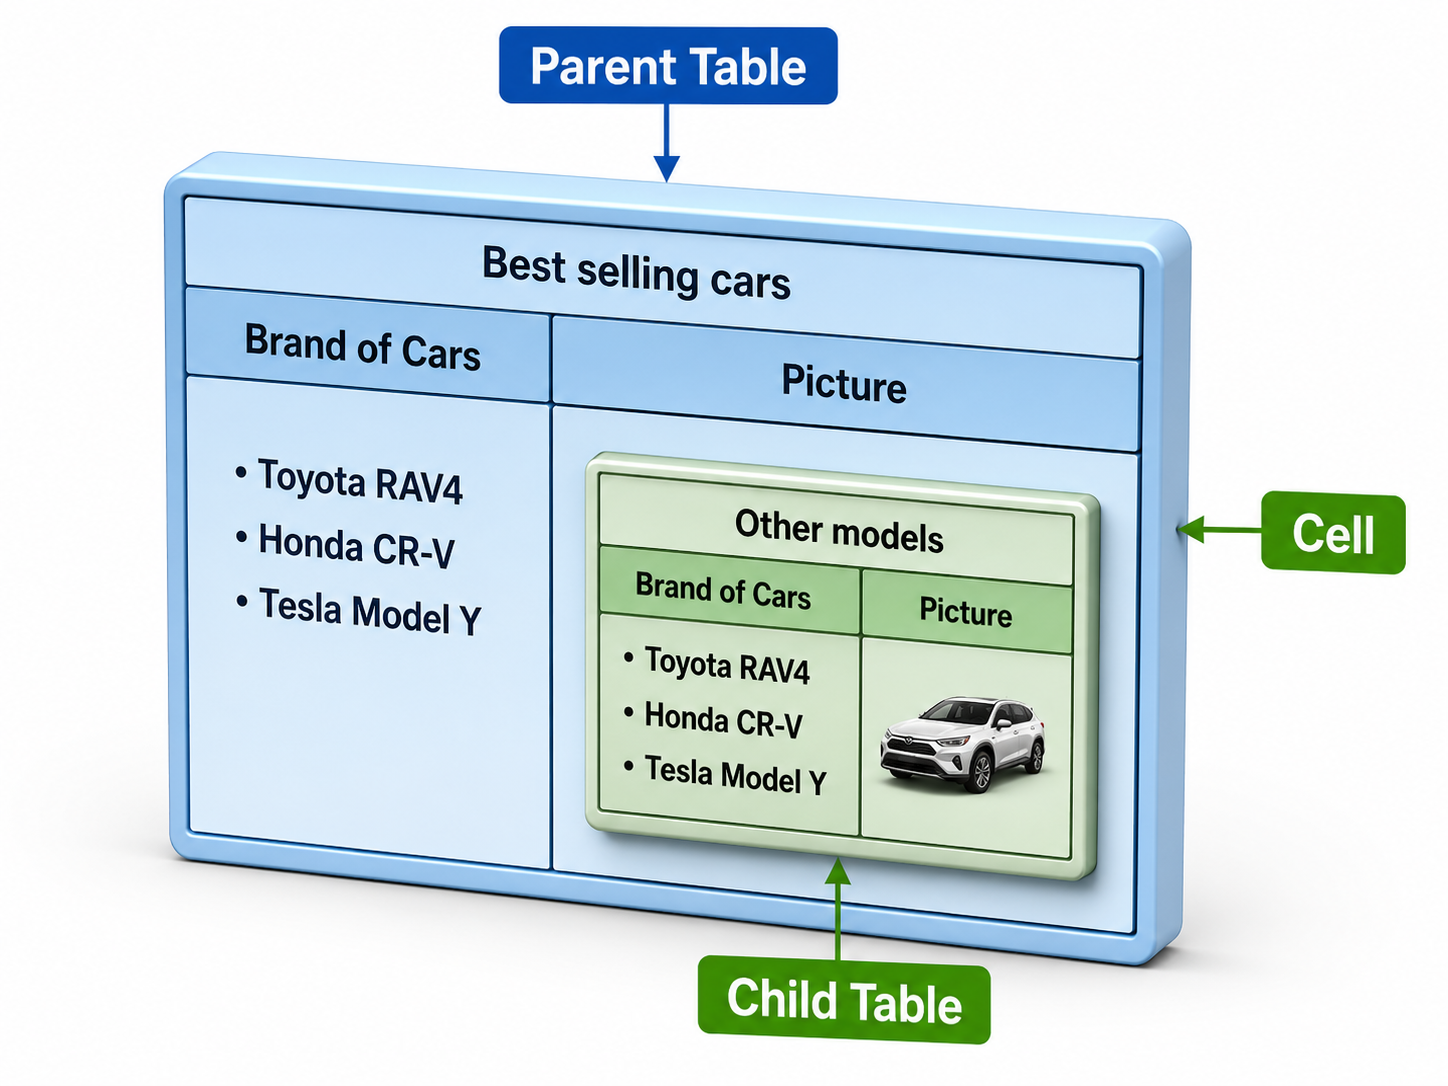
\includegraphics[width=0.95\linewidth,height=0.11\textheight,keepaspectratio]{chapters/Chapter04/topics/images/ex32_3d_nested_table_parent_child.png}
}{
\fbox{\parbox{0.90\linewidth}{\centering\vspace{0.45cm}
\textbf{চিত্র}\\[3pt]
File: \texttt{chapters/Chapter04/topics/images/ex32\_3d\_nested\_table\_parent\_child.png}
\vspace{0.45cm}}}
}
\captionof{figure}{Nested table: parent table-এর cell-এর ভিতরে child table}
\end{center}

\begin{keypointbox}{চিত্র ব্যাখ্যা}
Nested table-এ একটি বড় parent table-এর কোনো একটি cell-এর ভিতরে আরেকটি ছোট child table বসানো হয়। বইয়ের example-এ বিস্তারিত অংশের ভিতরে ছোট table ব্যবহার করা হয়েছে।
\end{keypointbox}

\begin{keypointbox}{চিত্র দেখে code লেখার ধাপ}
প্রথমে figure-এর total row ও column গুনবে। এরপর কোন cell একাধিক column জুড়ে আছে তা দেখে \texttt{colspan} এবং কোন cell একাধিক row জুড়ে আছে তা দেখে \texttt{rowspan} বসাবে। তারপর image, link, list বা nested table থাকলে সংশ্লিষ্ট tag cell-এর ভিতরে লিখবে।
\end{keypointbox}

\par\noindent{\color{purple!70!black}\bfseries\small কোড}\par\vspace{-4pt}
\begin{verbatim}
<!DOCTYPE html>
<html>
<head>
  <title>Table Inside Table</title>
</head>
<body>
<h3>বাইরের টেবিল (Parent Table)</h3>
<table border="2" cellpadding="10">
<tr>
  <th>নাম</th>
  <th>বিস্তারিত</th>
</tr>
<tr>
  <td>রাফি</td>
  <td>
    <!-- ভিতরের টেবিল শুরু -->
    <table border="1" cellpadding="5">
    <tr>
      <th>বিষয়</th>
      <th>নম্বর</th>
    </tr>
    <tr>
      <td>গণিত</td>
      <td>৮৫</td>
    </tr>
    <tr>
      <td>বিজ্ঞান</td>
      <td>৯০</td>
    </tr>
    </table>
    <!-- ভিতরের টেবিল শেষ -->
  </td>
</tr>
</table>
</body>
</html>
\end{verbatim}
\vspace{-6pt}

\subsubsection{Exercise 33: Student Subjects Table}

\begin{center}
\IfFileExists{chapters/Chapter04/topics/images/ex33_3d_student_subjects.png}{
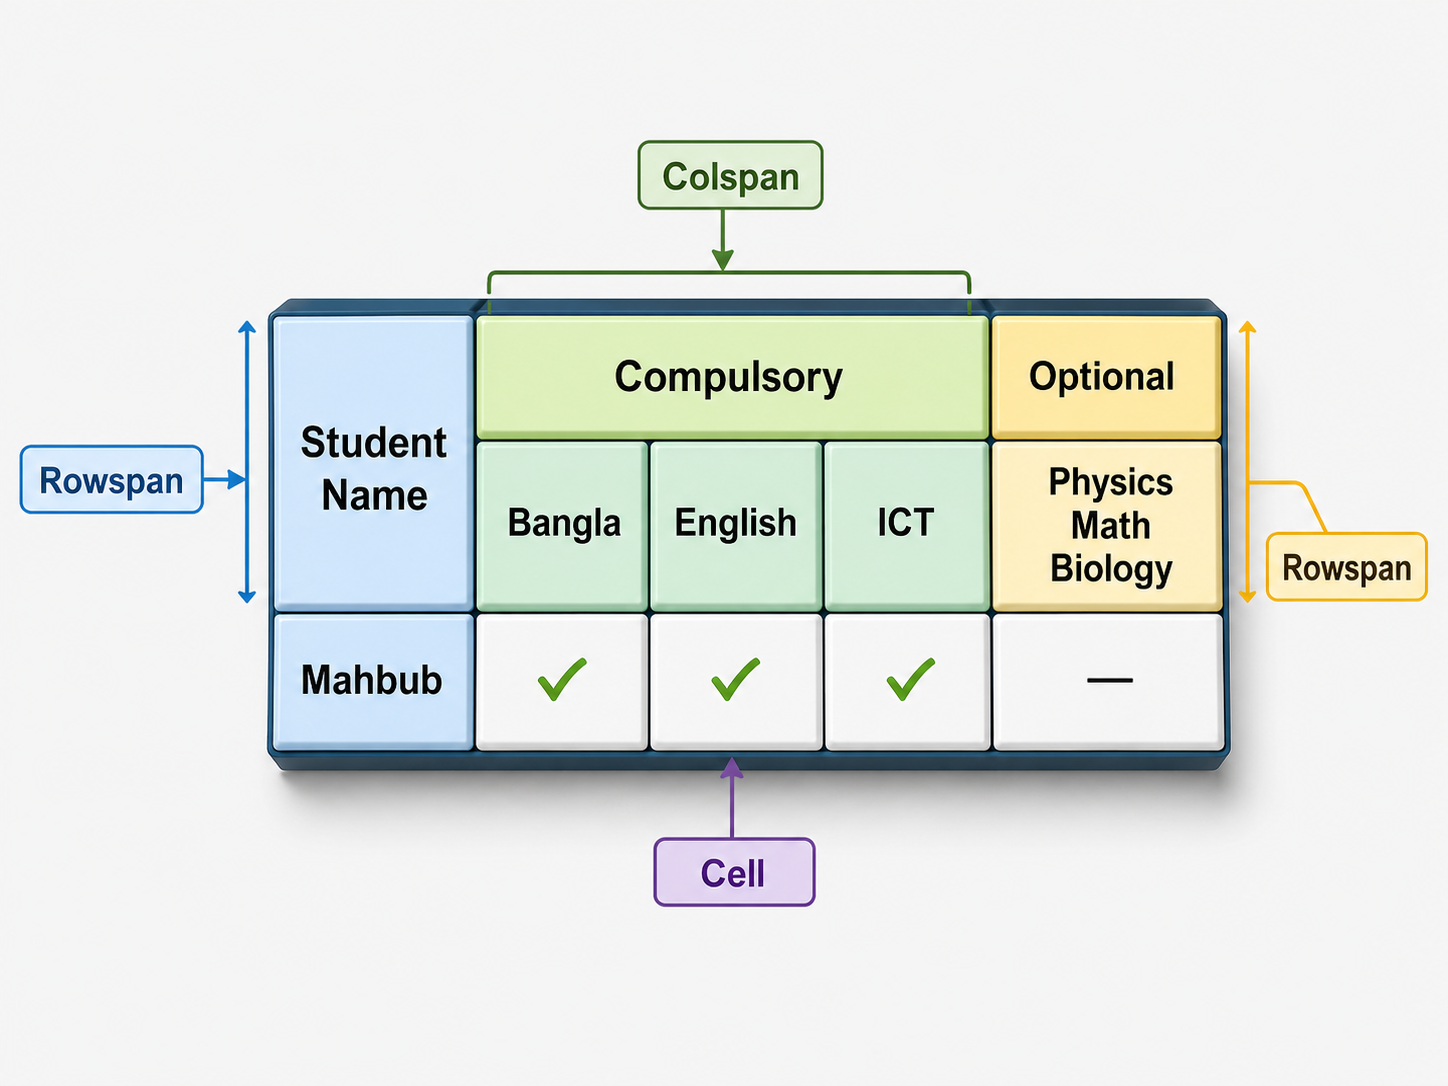
\includegraphics[width=0.95\linewidth,height=0.11\textheight,keepaspectratio]{chapters/Chapter04/topics/images/ex33_3d_student_subjects.png}
}{
\fbox{\parbox{0.90\linewidth}{\centering\vspace{0.45cm}
\textbf{চিত্র}\\[3pt]
File: \texttt{chapters/Chapter04/topics/images/ex33\_3d\_student\_subjects.png}
\vspace{0.45cm}}}
}
\captionof{figure}{Student Subjects table with rowspan and colspan}
\end{center}

\begin{keypointbox}{চিত্র ব্যাখ্যা}
Student Name এবং Optional heading দুই row জুড়ে আছে। Compulsory heading তিনটি subject column জুড়ে আছে। Mahbub ও tick mark cell-গুলো তিনটি optional subject row জুড়ে আছে।
\end{keypointbox}

\par\noindent{\color{purple!70!black}\bfseries\small কোড}\par\vspace{-4pt}
\begin{verbatim}
<!DOCTYPE html>
<html>
<head>
  <title>Student Subjects Table</title>
</head>
<body>
<table border="1" cellspacing="0">
<tr>
  <th rowspan="2">Student Name</th>
  <th colspan="3">Compulsory</th>
  <th rowspan="2">Optional</th>
</tr>
<tr>
  <td>Bangla</td>
  <td>English</td>
  <td>ICT</td>
</tr>
<tr>
  <th rowspan="3">Mahbub</th>
  <th rowspan="3">&#10003;</th>
  <th rowspan="3">&#10003;</th>
  <th rowspan="3">&#10003;</th>
  <td>Physics</td>
</tr>
<tr><td>Math</td></tr>
<tr><td>Biology</td></tr>
</table>
</body>
</html>
\end{verbatim}
\vspace{-6pt}

\subsubsection{Exercise 34: Science Fair Projects Table}

\begin{center}
\IfFileExists{chapters/Chapter04/topics/images/ex34_3d_science_fair_projects.png}{
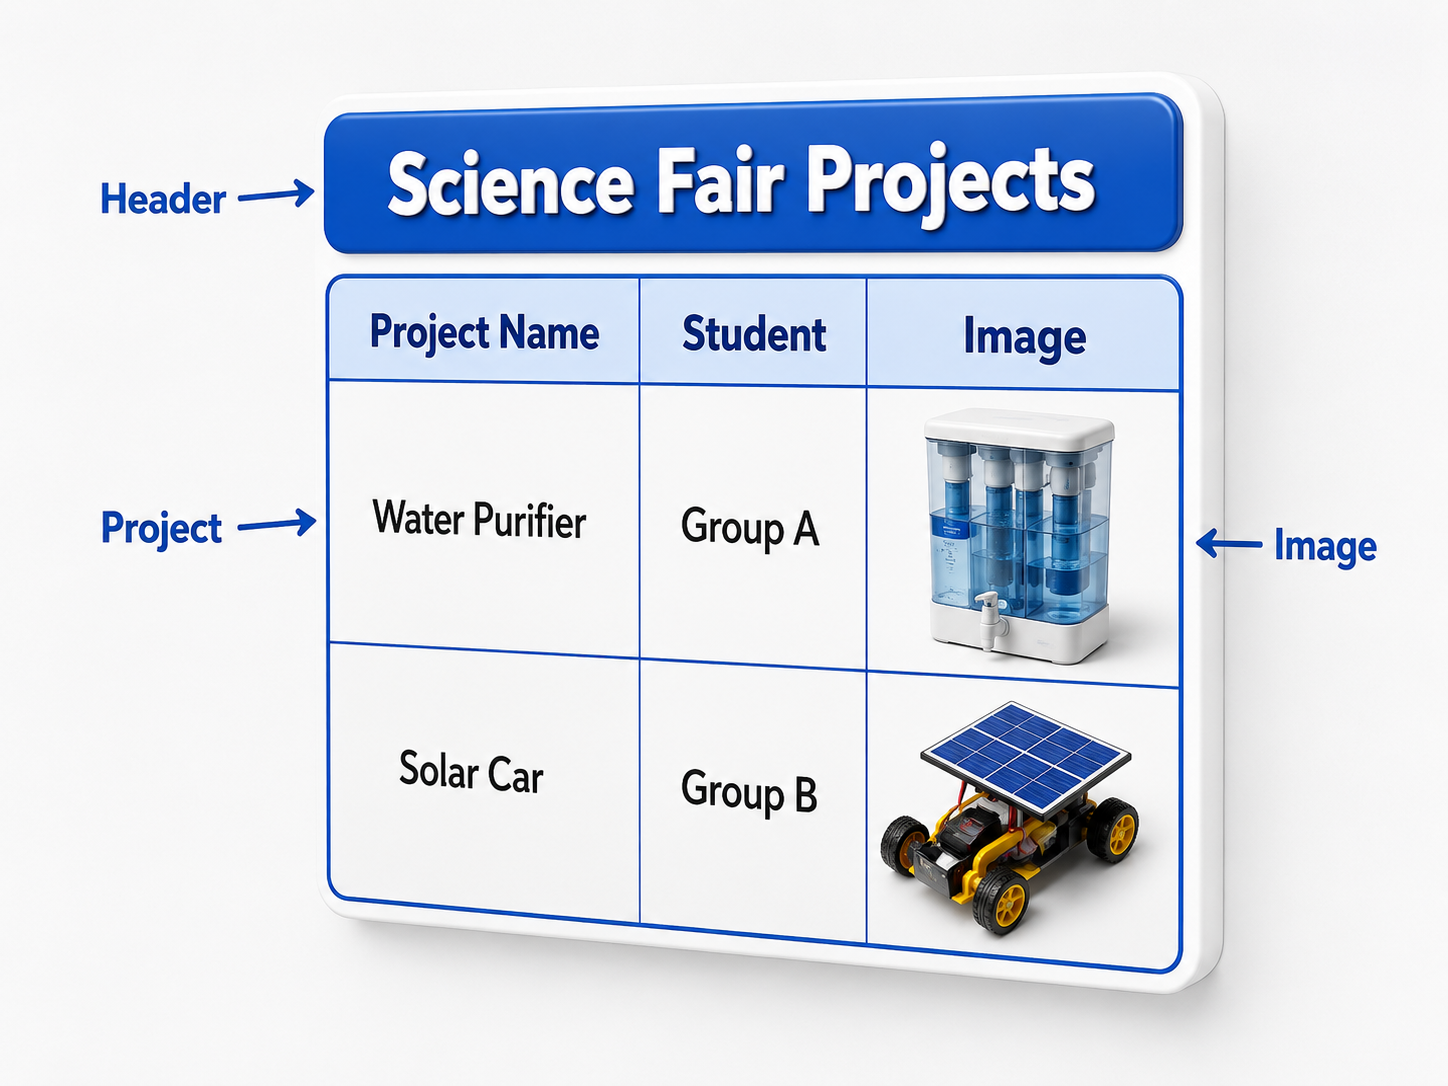
\includegraphics[width=0.95\linewidth,height=0.11\textheight,keepaspectratio]{chapters/Chapter04/topics/images/ex34_3d_science_fair_projects.png}
}{
\fbox{\parbox{0.90\linewidth}{\centering\vspace{0.45cm}
\textbf{চিত্র}\\[3pt]
File: \texttt{chapters/Chapter04/topics/images/ex34\_3d\_science\_fair\_projects.png}
\vspace{0.45cm}}}
}
\captionof{figure}{Science Fair Projects table with student/group and image}
\end{center}

\begin{keypointbox}{চিত্র ব্যাখ্যা}
চিত্রে Science Fair Projects heading-এর নিচে Project Name, Student এবং Image column আছে। প্রতিটি project row-তে project name, group/student label এবং project image দেওয়া হয়েছে।
\end{keypointbox}

\begin{keypointbox}{চিত্র দেখে code লেখার ধাপ}
প্রথমে heading লিখবে। এরপর তিনটি column identify করবে: Project Name, Student এবং Image। শেষ column-এ প্রতিটি project-এর জন্য \texttt{<img>} tag বসাবে।
\end{keypointbox}

\par\noindent{\color{purple!70!black}\bfseries\small কোড}\par\vspace{-4pt}
\begin{verbatim}
<!DOCTYPE html>
<html>
<head>
  <title>HTML Table Example</title>
</head>
<body>
<h2 align="center">Science Fair Projects</h2>
<table border="1" align="center" cellspacing="0" cellpadding="6">
<tr>
  <th>Project Name</th>
  <th>Student</th>
  <th>Image</th>
</tr>
<tr>
  <td>Water Purifier</td>
  <td>Group A</td>
  <td><img src="purifier.jpg" width="80" height="60" alt="Water Purifier"></td>
</tr>
<tr>
  <td>Solar Car</td>
  <td>Group B</td>
  <td><img src="solarcar.jpg" width="80" height="60" alt="Solar Car"></td>
</tr>
</table>
</body>
</html>
\end{verbatim}
\vspace{-6pt}

\subsubsection{Exercise 35: Group, Section and Club Table}

\begin{center}
\IfFileExists{chapters/Chapter04/topics/images/ex35_3d_group_section_club.png}{
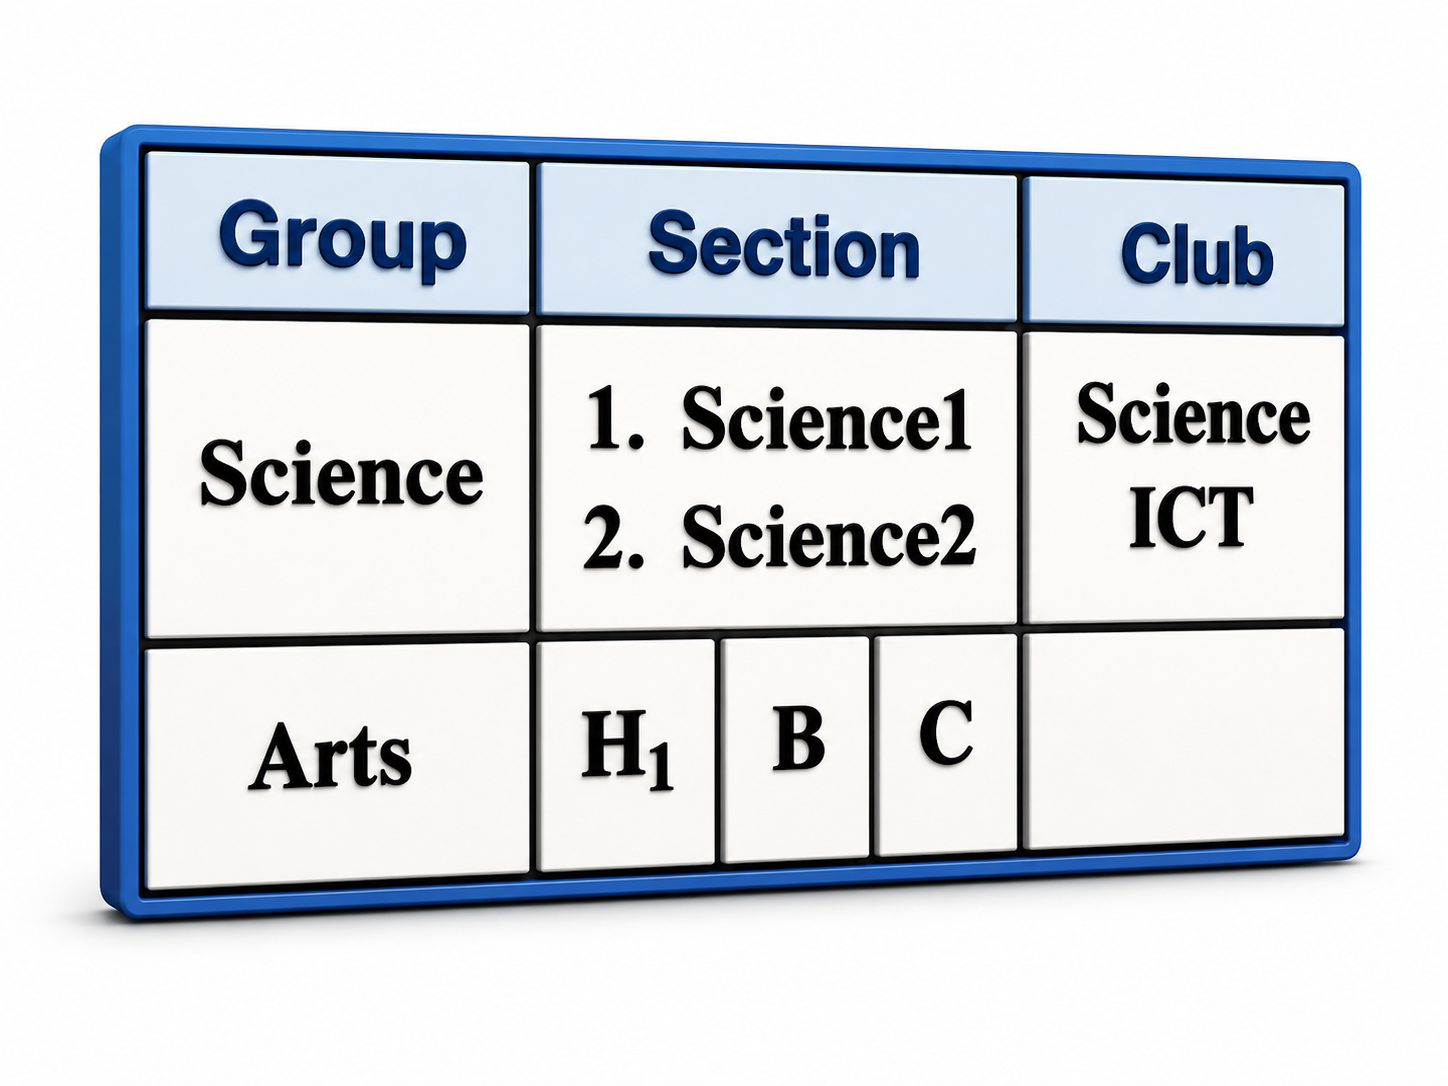
\includegraphics[width=0.95\linewidth,height=0.11\textheight,keepaspectratio]{chapters/Chapter04/topics/images/ex35_3d_group_section_club.png}
}{
\fbox{\parbox{0.90\linewidth}{\centering\vspace{0.45cm}
\textbf{চিত্র}\\[3pt]
File: \texttt{chapters/Chapter04/topics/images/ex35\_3d\_group\_section\_club.png}
\vspace{0.45cm}}}
}
\captionof{figure}{Group, Section and Club table with colspan, rowspan, sub and span}
\end{center}

\begin{keypointbox}{চিত্র ব্যাখ্যা}
Section heading তিনটি column জুড়ে আছে। Club cell দুই row জুড়ে আছে। Science row-তে Section অংশ তিনটি column জুড়ে text দেখানো হয়েছে। Arts row-তে H\textsubscript{1}, B এবং C আলাদা cell-এ আছে।
\end{keypointbox}

\begin{keypointbox}{চিত্র দেখে code লেখার ধাপ}
প্রথমে figure-এর total row ও column গুনবে। এরপর কোন cell একাধিক column জুড়ে আছে তা দেখে \texttt{colspan} এবং কোন cell একাধিক row জুড়ে আছে তা দেখে \texttt{rowspan} বসাবে। তারপর image, link, list বা nested table থাকলে সংশ্লিষ্ট tag cell-এর ভিতরে লিখবে।
\end{keypointbox}

\par\noindent{\color{purple!70!black}\bfseries\small কোড}\par\vspace{-4pt}
\begin{verbatim}
<!DOCTYPE html>
<html>
<head>
  <title>Group Table</title>
</head>
<body>
<table border="1" cellspacing="0" cellpadding="5">
<tr>
  <th>Group</th>
  <th colspan="3">Section</th>
  <th rowspan="2"><u>Club</u><br>
    <span style="font-weight:normal;">Science<br>ICT</span>
  </th>
</tr>
<tr>
  <td>Science</td>
  <td colspan="3">1. Science1<br>2. Science2</td>
</tr>
<tr>
  <td>Arts</td>
  <td>H<sub>1</sub></td>
  <td>B</td>
  <td>C</td>
  <td></td>
</tr>
</table>
</body>
</html>
\end{verbatim}
\vspace{-6pt}

\subsubsection{Exercise 36: Delight Restaurant Table}

\begin{center}
\IfFileExists{chapters/Chapter04/topics/images/ex36_3d_delight_restaurant.png}{
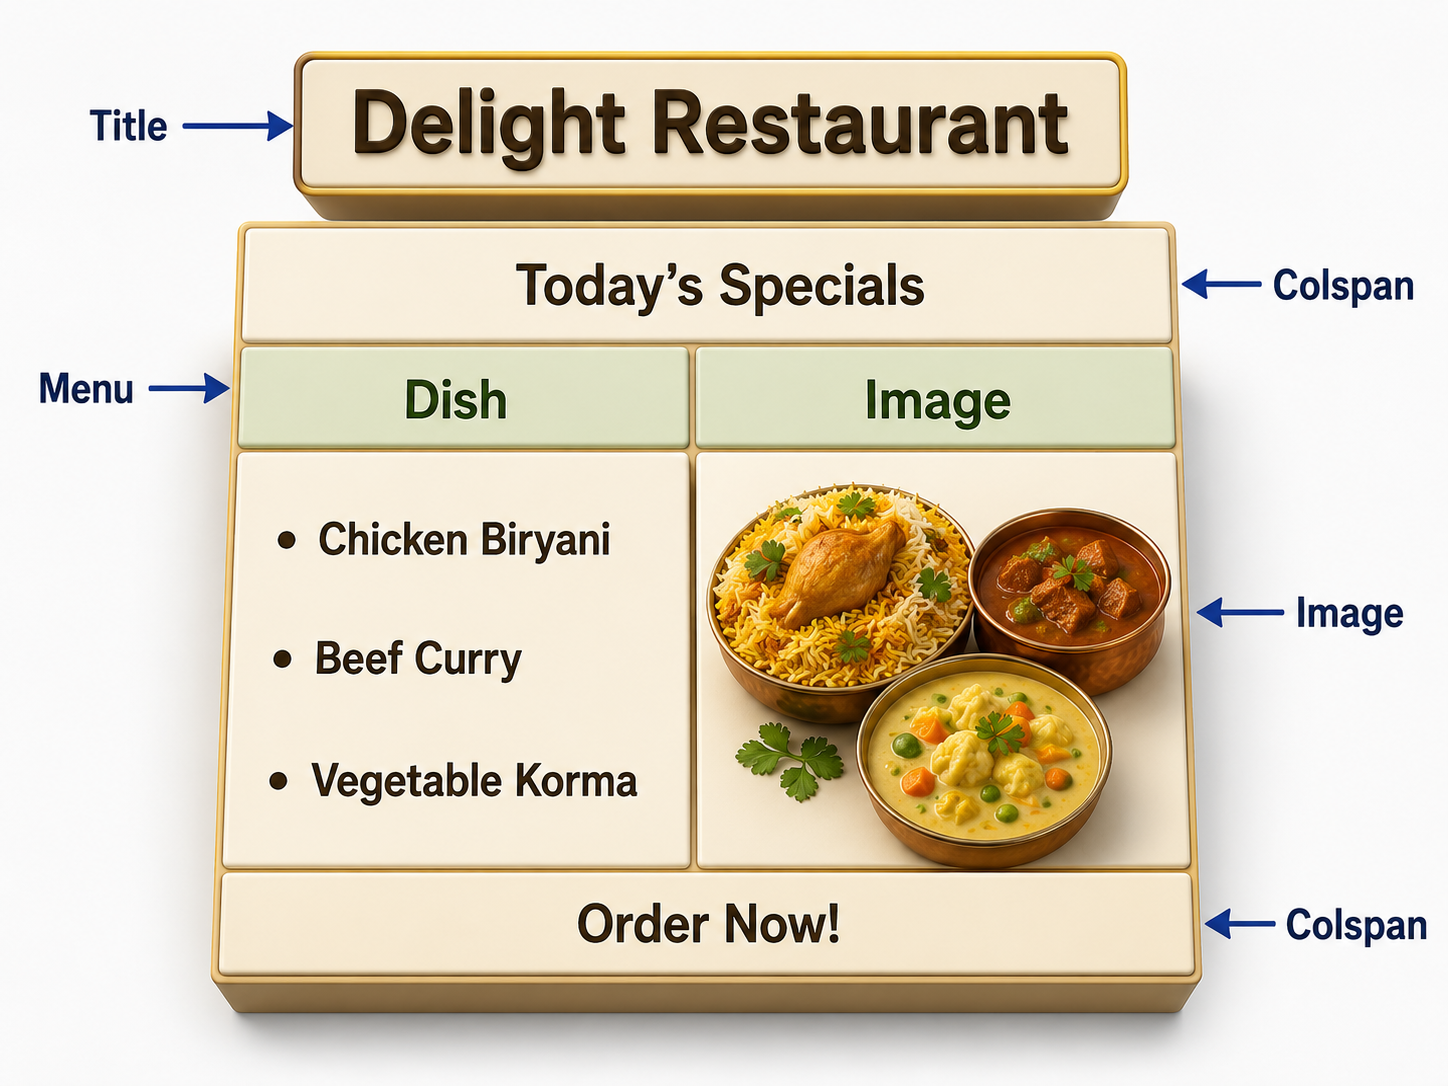
\includegraphics[width=0.95\linewidth,height=0.11\textheight,keepaspectratio]{chapters/Chapter04/topics/images/ex36_3d_delight_restaurant.png}
}{
\fbox{\parbox{0.90\linewidth}{\centering\vspace{0.45cm}
\textbf{চিত্র}\\[3pt]
File: \texttt{chapters/Chapter04/topics/images/ex36\_3d\_delight\_restaurant.png}
\vspace{0.45cm}}}
}
\captionof{figure}{Delight Restaurant table with food image and order row}
\end{center}

\begin{keypointbox}{চিত্র ব্যাখ্যা}
এই table-এ Today's Specials এবং Order Now row দুই column জুড়ে আছে। Dish cell-এ line break দিয়ে item list দেখানো হয়েছে এবং Image cell-এ food image রাখা হয়েছে।
\end{keypointbox}

\par\noindent{\color{purple!70!black}\bfseries\small কোড}\par\vspace{-4pt}
\begin{verbatim}
<!DOCTYPE html>
<html>
<head>
  <title>HTML Table Example</title>
</head>
<body>
<h2 align="center">Delight Restaurant</h2>
<table border="1" align="center" cellspacing="0" cellpadding="8">
<tr>
  <th colspan="2">Today's Specials</th>
</tr>
<tr>
  <th>Dish</th>
  <th>Image</th>
</tr>
<tr>
  <td>• Chicken Biryani<br>• Beef Curry<br>• Vegetable Korma</td>
  <td><img src="food.jpg" width="100" height="80" alt="Food"></td>
</tr>
<tr>
  <td colspan="2" align="center">Order Now!</td>
</tr>
</table>
</body>
</html>
\end{verbatim}
\vspace{-6pt}

% =========================================================
% Extra HSC ICT Board-Style Mixed HTML Table Examples
% Add this file after the main Table in HTML topic.
% Image labels should be short English labels; explanation remains in Bangla.
% =========================================================

\subsection{আরও Board-Style Mixed HTML Table Practice}

\begin{boardbox}{কেন এই অংশ গুরুত্বপূর্ণ}
HSC ICT practical/CQ-তে HTML table থেকে সাধারণত চিত্র দেখে code লিখতে বলা হয়। এসব প্রশ্নে \texttt{rowspan}, \texttt{colspan}, \texttt{image}, \texttt{hyperlink}, \texttt{list}, nested table, alignment ইত্যাদি মিশ্রভাবে থাকতে পারে। নিচের উদাহরণগুলো board-style practice হিসেবে তৈরি করা হয়েছে।
\end{boardbox}


\subsubsection{Example 55: Admission Schedule with Logo, Link, Rowspan and Colspan}

\begin{center}
\IfFileExists{chapters/Chapter04/topics/images/board_ex55_3d_admission_schedule.png}{
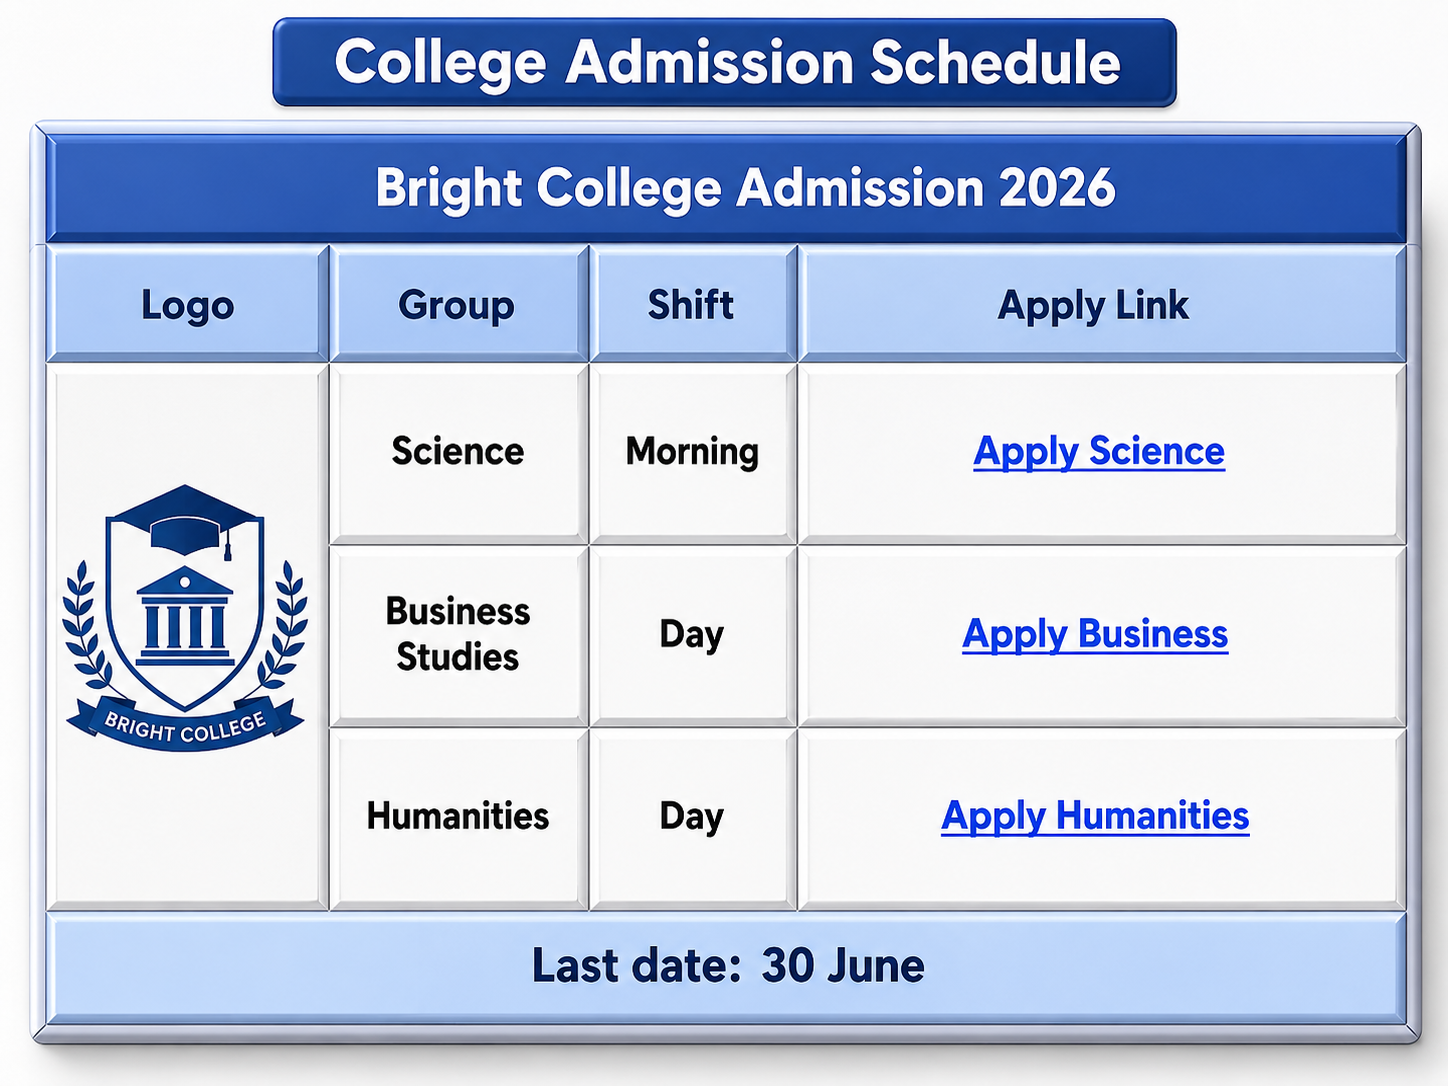
\includegraphics[width=0.95\linewidth,height=0.11\textheight,keepaspectratio]{chapters/Chapter04/topics/images/board_ex55_3d_admission_schedule.png}
}{
\fbox{\parbox{0.90\linewidth}{\centering\vspace{0.45cm}
\textbf{চিত্র}\\[3pt]
File: \texttt{chapters/Chapter04/topics/images/board\_ex55\_3d\_admission\_schedule.png}
\vspace{0.45cm}}}
}
\captionof{figure}{Admission Schedule with Logo, Link, Rowspan and Colspan}
\end{center}

\begin{keypointbox}{চিত্র ব্যাখ্যা}
এই example-এ logo image-এর জন্য rowspan, Apply Link অংশে colspan এবং শেষ row-তে full-width notice ব্যবহার করা হয়েছে।
\end{keypointbox}

\begin{keypointbox}{চিত্র দেখে code লেখার ধাপ}
প্রথমে figure-এর total row ও column গুনবে। এরপর কোন cell একাধিক column জুড়ে আছে তা দেখে \texttt{colspan} এবং কোন cell একাধিক row জুড়ে আছে তা দেখে \texttt{rowspan} বসাবে। তারপর image, link, list বা nested table থাকলে সংশ্লিষ্ট tag cell-এর ভিতরে লিখবে।
\end{keypointbox}

\par\noindent{\color{purple!70!black}\bfseries\small কোড}\par\vspace{-4pt}
\begin{verbatim}
<!DOCTYPE html>
<html>
<head>
  <title>HTML Table Example</title>
</head>
<body>
<table border="1" cellspacing="0" cellpadding="6" align="center">
  <caption><b>College Admission Schedule</b></caption>
  <tr>
    <th colspan="5">Bright College Admission 2026</th>
  </tr>
  <tr>
    <th>Logo</th>
    <th>Group</th>
    <th>Shift</th>
    <th colspan="2">Apply Link</th>
  </tr>
  <tr>
    <td rowspan="3"><img src="college_logo.png" width="80" height="80" alt="College Logo"></td>
    <td>Science</td>
    <td>Morning</td>
    <td colspan="2"><a href="apply_science.html">Apply Science</a></td>
  </tr>
  <tr>
    <td>Business Studies</td>
    <td>Day</td>
    <td colspan="2"><a href="apply_business.html">Apply Business</a></td>
  </tr>
  <tr>
    <td>Humanities</td>
    <td>Day</td>
    <td colspan="2"><a href="apply_humanities.html">Apply Humanities</a></td>
  </tr>
  <tr>
    <td colspan="5" align="center">Last date: 30 June</td>
  </tr>
</table>
</body>
</html>
\end{verbatim}
\vspace{-6pt}

\begin{keypointbox}{Board technique}
প্রথমে মোট row ও column গুনবে। তারপর কোন cell horizontal merge হলে \texttt{colspan} এবং vertical merge হলে \texttt{rowspan} ব্যবহার করবে। image-এর জন্য \texttt{<img>} এবং link-এর জন্য \texttt{<a>} tag ব্যবহার করবে।
\end{keypointbox}


\subsubsection{Example 56: Student Result with Compulsory and Optional Subjects}

\begin{center}
\IfFileExists{chapters/Chapter04/topics/images/board_ex56_3d_student_result_mixed.png}{
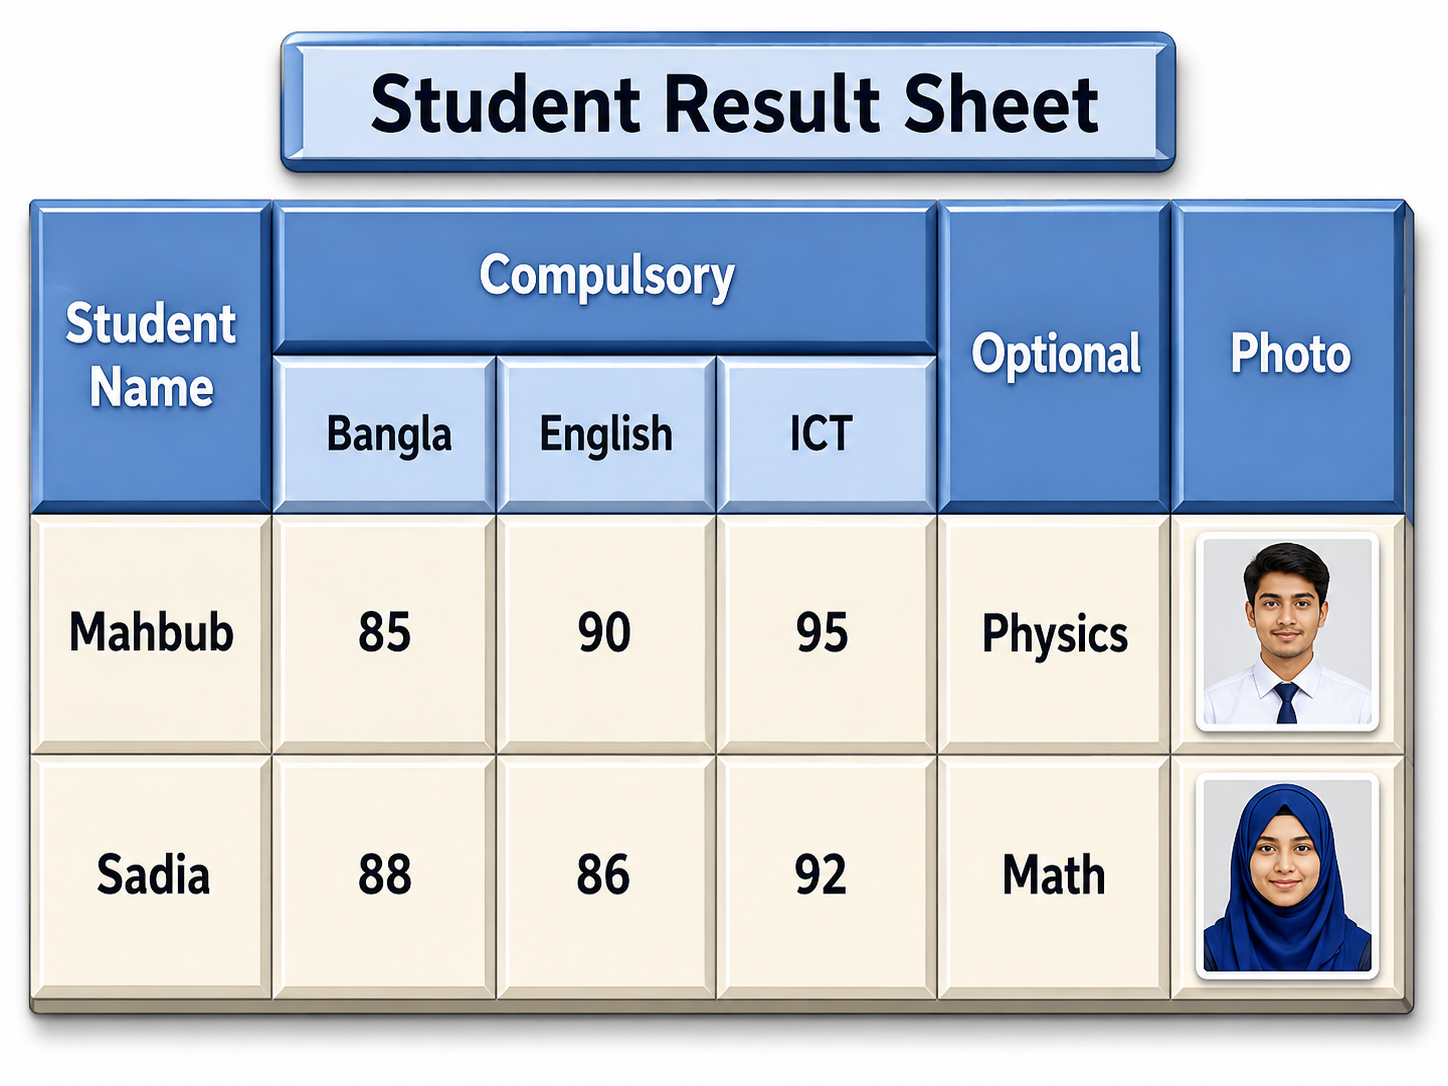
\includegraphics[width=0.95\linewidth,height=0.11\textheight,keepaspectratio]{chapters/Chapter04/topics/images/board_ex56_3d_student_result_mixed.png}
}{
\fbox{\parbox{0.90\linewidth}{\centering\vspace{0.45cm}
\textbf{চিত্র}\\[3pt]
File: \texttt{chapters/Chapter04/topics/images/board\_ex56\_3d\_student\_result\_mixed.png}
\vspace{0.45cm}}}
}
\captionof{figure}{Student Result with Compulsory and Optional Subjects}
\end{center}

\begin{keypointbox}{চিত্র ব্যাখ্যা}
এখানে Student Name, Optional ও Photo header দুই row জুড়ে আছে; Compulsory heading তিনটি column জুড়ে আছে।
\end{keypointbox}

\par\noindent{\color{purple!70!black}\bfseries\small কোড}\par\vspace{-4pt}
\begin{verbatim}
<!DOCTYPE html>
<html>
<head>
  <title>HTML Table Example</title>
</head>
<body>
<table border="1" cellspacing="0" cellpadding="5" align="center">
  <caption><b>Student Result Sheet</b></caption>
  <tr>
    <th rowspan="2">Student Name</th>
    <th colspan="3">Compulsory</th>
    <th rowspan="2">Optional</th>
    <th rowspan="2">Photo</th>
  </tr>
  <tr>
    <th>Bangla</th>
    <th>English</th>
    <th>ICT</th>
  </tr>
  <tr>
    <td>Mahbub</td>
    <td>85</td>
    <td>90</td>
    <td>95</td>
    <td>Physics</td>
    <td><img src="mahbub.jpg" width="60" height="70" alt="Mahbub"></td>
  </tr>
  <tr>
    <td>Sadia</td>
    <td>88</td>
    <td>86</td>
    <td>92</td>
    <td>Math</td>
    <td><img src="sadia.jpg" width="60" height="70" alt="Sadia"></td>
  </tr>
</table>
</body>
</html>
\end{verbatim}
\vspace{-6pt}

\begin{keypointbox}{Board technique}
প্রথমে মোট row ও column গুনবে। তারপর কোন cell horizontal merge হলে \texttt{colspan} এবং vertical merge হলে \texttt{rowspan} ব্যবহার করবে। image-এর জন্য \texttt{<img>} এবং link-এর জন্য \texttt{<a>} tag ব্যবহার করবে।
\end{keypointbox}


\subsubsection{Example 57: Product Catalog with Product Image and Buy Link}

\begin{center}
\IfFileExists{chapters/Chapter04/topics/images/board_ex57_3d_product_catalog_link.png}{
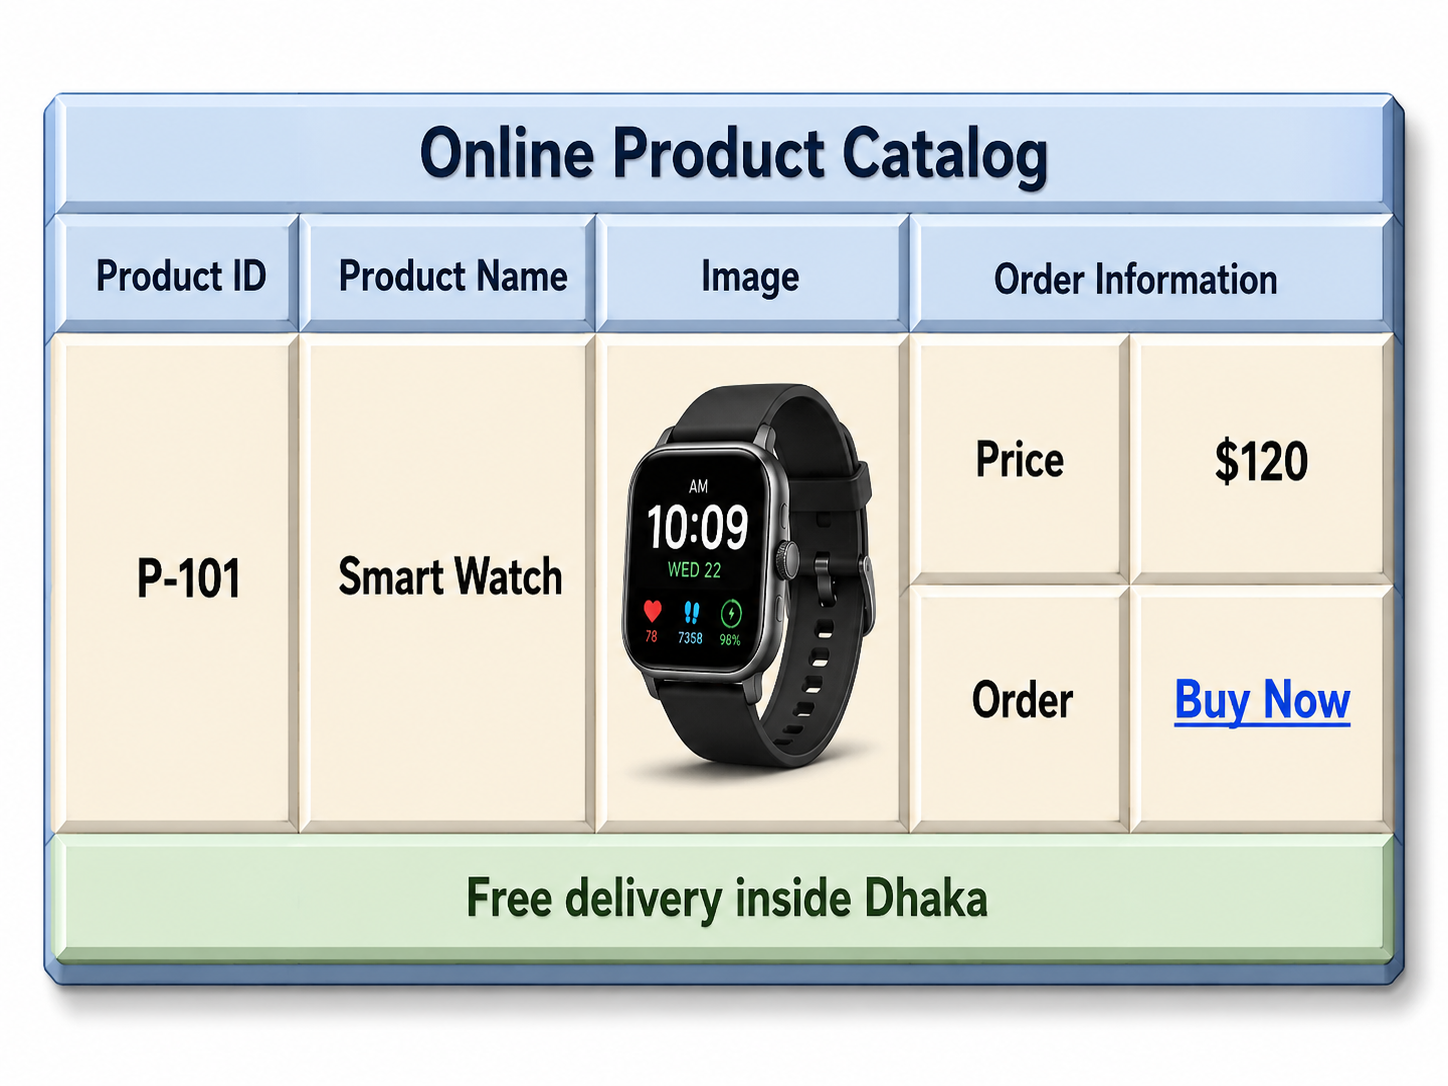
\includegraphics[width=0.95\linewidth,height=0.11\textheight,keepaspectratio]{chapters/Chapter04/topics/images/board_ex57_3d_product_catalog_link.png}
}{
\fbox{\parbox{0.90\linewidth}{\centering\vspace{0.45cm}
\textbf{চিত্র}\\[3pt]
File: \texttt{chapters/Chapter04/topics/images/board\_ex57\_3d\_product\_catalog\_link.png}
\vspace{0.45cm}}}
}
\captionof{figure}{Product Catalog with Product Image and Buy Link}
\end{center}

\begin{keypointbox}{চিত্র ব্যাখ্যা}
Product ID, Name ও Image দুই row জুড়ে রাখা হয়েছে। Order Information দুই column জুড়ে আছে।
\end{keypointbox}

\begin{keypointbox}{চিত্র দেখে code লেখার ধাপ}
প্রথমে figure-এর total row ও column গুনবে। এরপর কোন cell একাধিক column জুড়ে আছে তা দেখে \texttt{colspan} এবং কোন cell একাধিক row জুড়ে আছে তা দেখে \texttt{rowspan} বসাবে। তারপর image, link, list বা nested table থাকলে সংশ্লিষ্ট tag cell-এর ভিতরে লিখবে।
\end{keypointbox}

\par\noindent{\color{purple!70!black}\bfseries\small কোড}\par\vspace{-4pt}
\begin{verbatim}
<!DOCTYPE html>
<html>
<head>
  <title>HTML Table Example</title>
</head>
<body>
<table border="1" cellspacing="0" cellpadding="6" align="center">
  <caption><b>Online Product Catalog</b></caption>
  <tr>
    <th>Product ID</th>
    <th>Product Name</th>
    <th>Image</th>
    <th colspan="2">Order Information</th>
  </tr>
  <tr>
    <td rowspan="2">P-101</td>
    <td rowspan="2">Smart Watch</td>
    <td rowspan="2"><img src="watch.jpg" width="90" height="80" alt="Watch"></td>
    <td>Price</td>
    <td>$120</td>
  </tr>
  <tr>
    <td>Order</td>
    <td><a href="order_watch.html">Buy Now</a></td>
  </tr>
  <tr>
    <td colspan="5" align="center">Free delivery inside Dhaka</td>
  </tr>
</table>
</body>
</html>
\end{verbatim}
\vspace{-6pt}

\begin{keypointbox}{Board technique}
প্রথমে মোট row ও column গুনবে। তারপর কোন cell horizontal merge হলে \texttt{colspan} এবং vertical merge হলে \texttt{rowspan} ব্যবহার করবে। image-এর জন্য \texttt{<img>} এবং link-এর জন্য \texttt{<a>} tag ব্যবহার করবে।
\end{keypointbox}


\subsubsection{Example 58: Hospital Information Table with Picture and Emergency Link}

\begin{center}
\IfFileExists{chapters/Chapter04/topics/images/board_ex58_3d_hospital_info_table.png}{
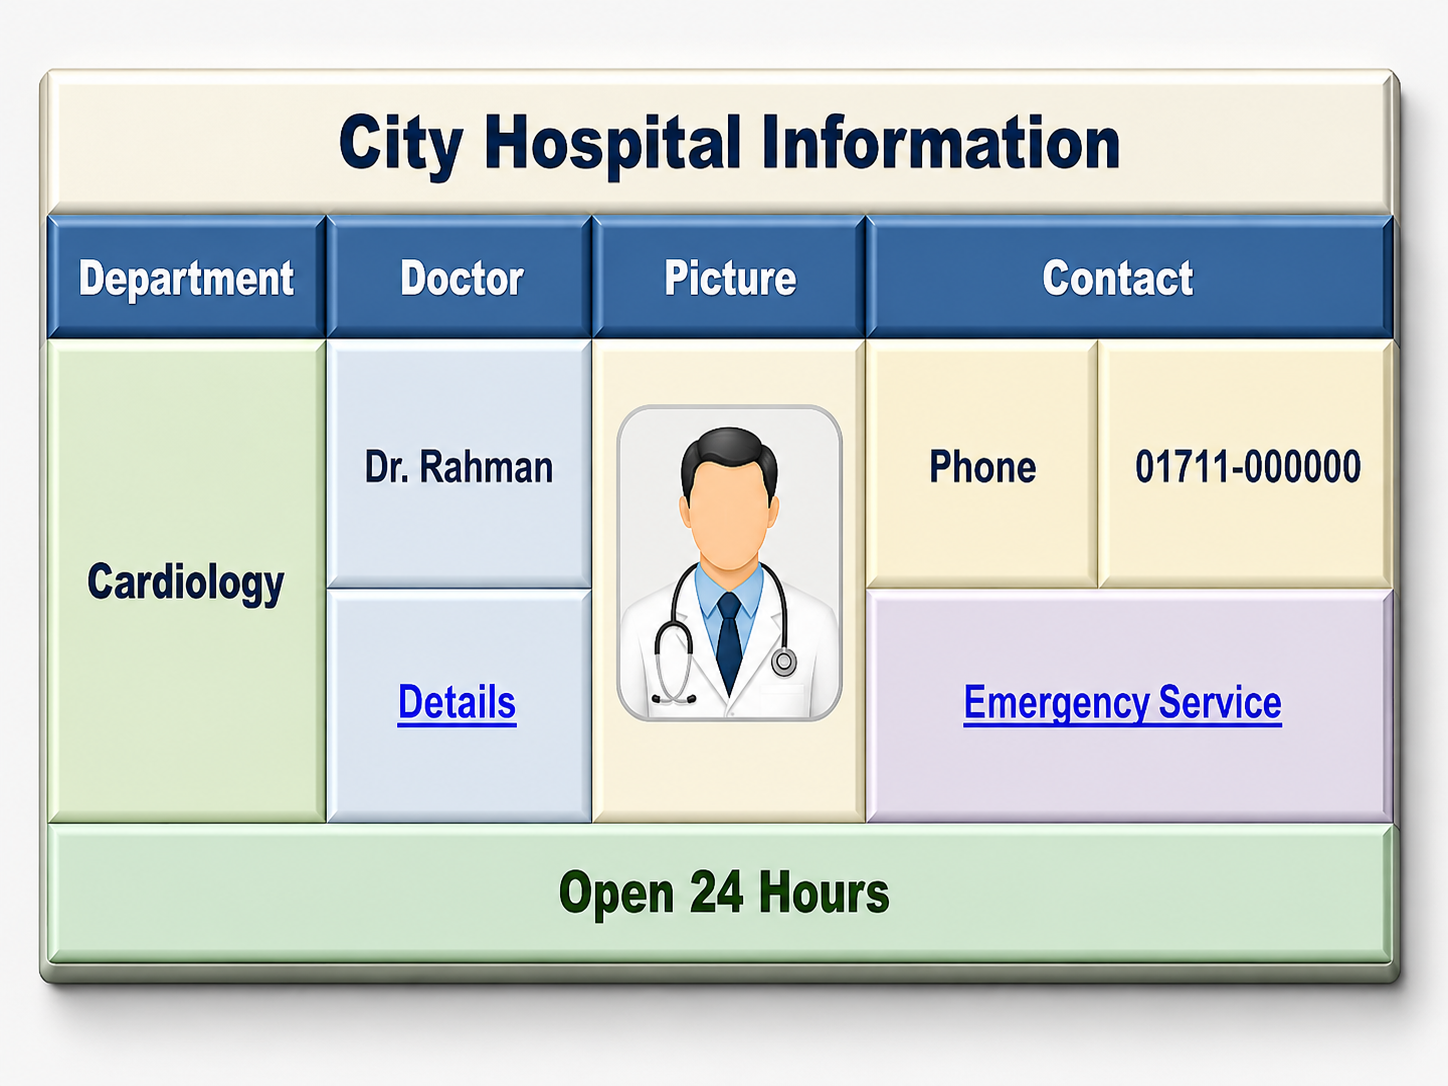
\includegraphics[width=0.95\linewidth,height=0.11\textheight,keepaspectratio]{chapters/Chapter04/topics/images/board_ex58_3d_hospital_info_table.png}
}{
\fbox{\parbox{0.90\linewidth}{\centering\vspace{0.45cm}
\textbf{চিত্র}\\[3pt]
File: \texttt{chapters/Chapter04/topics/images/board\_ex58\_3d\_hospital\_info\_table.png}
\vspace{0.45cm}}}
}
\captionof{figure}{Hospital Information Table with Picture and Emergency Link}
\end{center}

\begin{keypointbox}{চিত্র ব্যাখ্যা}
Cardiology cell এবং doctor image দুই row জুড়ে আছে। Emergency Service link দুইটি contact column জুড়ে দেওয়া হয়েছে।
\end{keypointbox}

\par\noindent{\color{purple!70!black}\bfseries\small কোড}\par\vspace{-4pt}
\begin{verbatim}
<!DOCTYPE html>
<html>
<head>
  <title>HTML Table Example</title>
</head>
<body>
<table border="1" cellspacing="0" cellpadding="6" align="center">
  <caption><b>City Hospital Information</b></caption>
  <tr>
    <th>Department</th>
    <th>Doctor</th>
    <th>Picture</th>
    <th colspan="2">Contact</th>
  </tr>
  <tr>
    <td rowspan="2">Cardiology</td>
    <td>Dr. Rahman</td>
    <td rowspan="2"><img src="doctor.jpg" width="80" height="90" alt="Doctor"></td>
    <td>Phone</td>
    <td>01711-000000</td>
  </tr>
  <tr>
    <td><a href="cardiology.html">Details</a></td>
    <td colspan="2"><a href="emergency.html">Emergency Service</a></td>
  </tr>
  <tr>
    <td colspan="5" align="center">Open 24 Hours</td>
  </tr>
</table>
</body>
</html>
\end{verbatim}
\vspace{-6pt}

\begin{keypointbox}{Board technique}
প্রথমে মোট row ও column গুনবে। তারপর কোন cell horizontal merge হলে \texttt{colspan} এবং vertical merge হলে \texttt{rowspan} ব্যবহার করবে। image-এর জন্য \texttt{<img>} এবং link-এর জন্য \texttt{<a>} tag ব্যবহার করবে।
\end{keypointbox}


\subsubsection{Example 59: Tourism Table with Place Image and Website Link}

\begin{center}
\IfFileExists{chapters/Chapter04/topics/images/board_ex59_3d_tourism_places_link.png}{
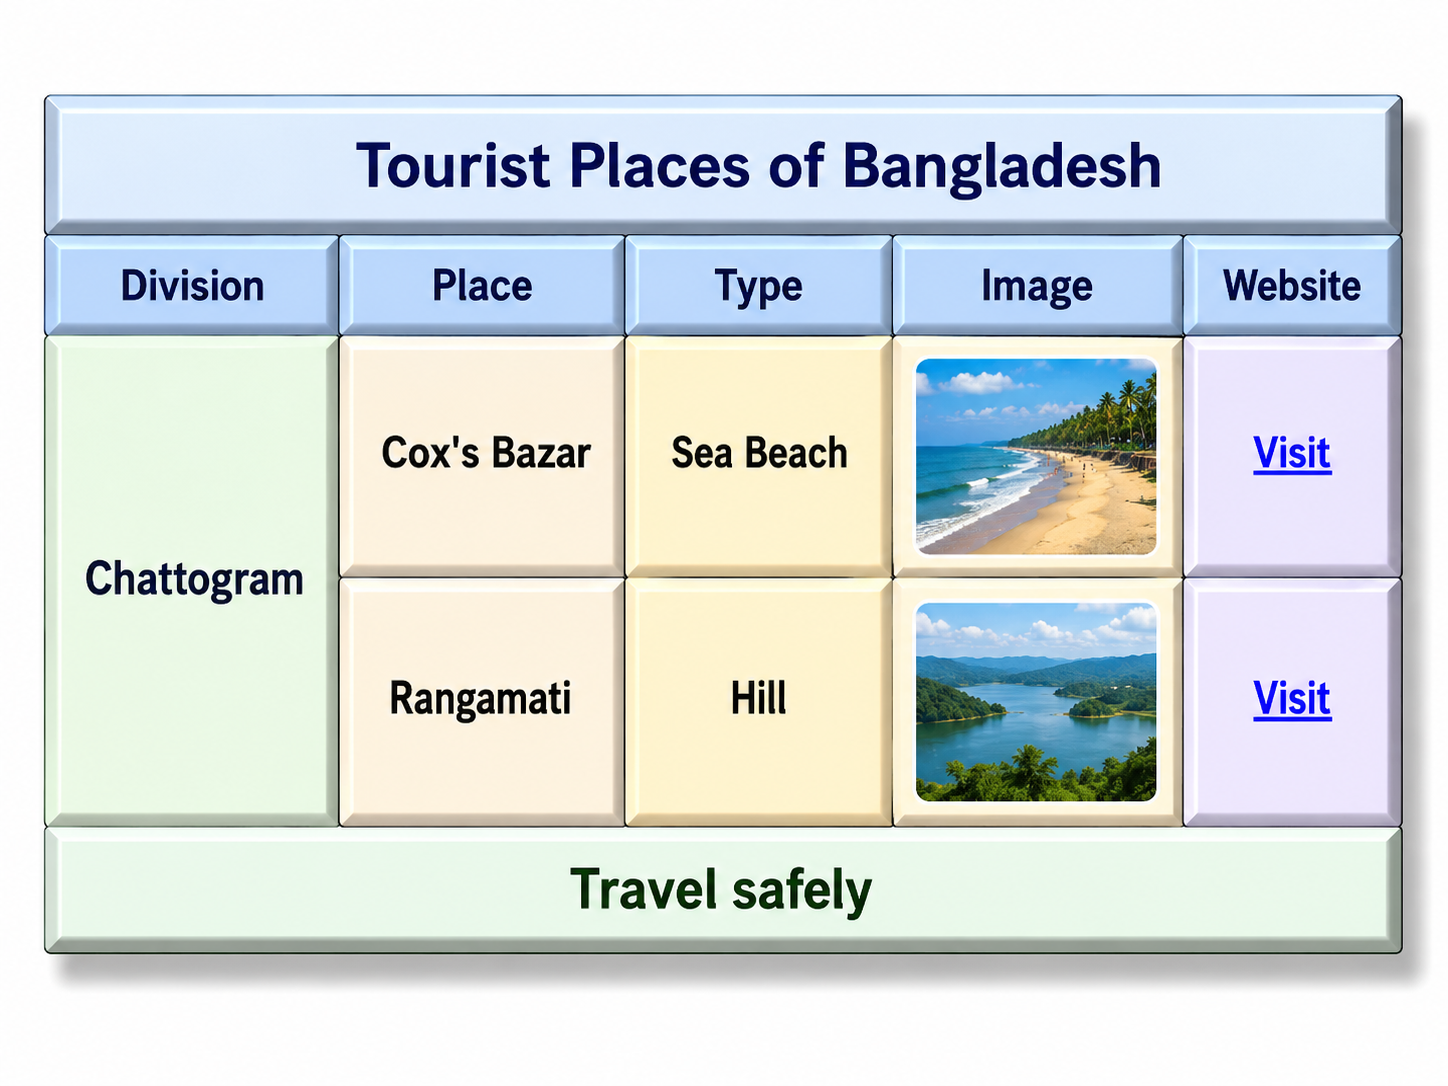
\includegraphics[width=0.95\linewidth,height=0.11\textheight,keepaspectratio]{chapters/Chapter04/topics/images/board_ex59_3d_tourism_places_link.png}
}{
\fbox{\parbox{0.90\linewidth}{\centering\vspace{0.45cm}
\textbf{চিত্র}\\[3pt]
File: \texttt{chapters/Chapter04/topics/images/board\_ex59\_3d\_tourism\_places\_link.png}
\vspace{0.45cm}}}
}
\captionof{figure}{Tourism Table with Place Image and Website Link}
\end{center}

\begin{keypointbox}{চিত্র ব্যাখ্যা}
Division cell rowspan দিয়ে দুই place-এর জন্য common করা হয়েছে। প্রতিটি place-এর image ও link আলাদা cell-এ আছে।
\end{keypointbox}

\begin{keypointbox}{চিত্র দেখে code লেখার ধাপ}
প্রথমে figure-এর total row ও column গুনবে। এরপর কোন cell একাধিক column জুড়ে আছে তা দেখে \texttt{colspan} এবং কোন cell একাধিক row জুড়ে আছে তা দেখে \texttt{rowspan} বসাবে। তারপর image, link, list বা nested table থাকলে সংশ্লিষ্ট tag cell-এর ভিতরে লিখবে।
\end{keypointbox}

\par\noindent{\color{purple!70!black}\bfseries\small কোড}\par\vspace{-4pt}
\begin{verbatim}
<!DOCTYPE html>
<html>
<head>
  <title>HTML Table Example</title>
</head>
<body>
<table border="1" cellspacing="0" cellpadding="5" align="center">
  <caption><b>Tourist Places of Bangladesh</b></caption>
  <tr>
    <th>Division</th>
    <th>Place</th>
    <th>Type</th>
    <th>Image</th>
    <th>Website</th>
  </tr>
  <tr>
    <td rowspan="2">Chattogram</td>
    <td>Cox's Bazar</td>
    <td>Sea Beach</td>
    <td><img src="cox.jpg" width="80" height="60" alt="Cox's Bazar"></td>
    <td><a href="cox.html">Visit</a></td>
  </tr>
  <tr>
    <td>Rangamati</td>
    <td>Hill</td>
    <td><img src="rangamati.jpg" width="80" height="60" alt="Rangamati"></td>
    <td><a href="rangamati.html">Visit</a></td>
  </tr>
  <tr>
    <td colspan="5" align="center">Travel safely</td>
  </tr>
</table>
</body>
</html>
\end{verbatim}
\vspace{-6pt}

\begin{keypointbox}{Board technique}
প্রথমে মোট row ও column গুনবে। তারপর কোন cell horizontal merge হলে \texttt{colspan} এবং vertical merge হলে \texttt{rowspan} ব্যবহার করবে। image-এর জন্য \texttt{<img>} এবং link-এর জন্য \texttt{<a>} tag ব্যবহার করবে।
\end{keypointbox}


\subsubsection{Example 60: Course Plan Table with List, Link and Colspan}

\begin{center}
\IfFileExists{chapters/Chapter04/topics/images/board_ex60_3d_course_plan_list_link.png}{
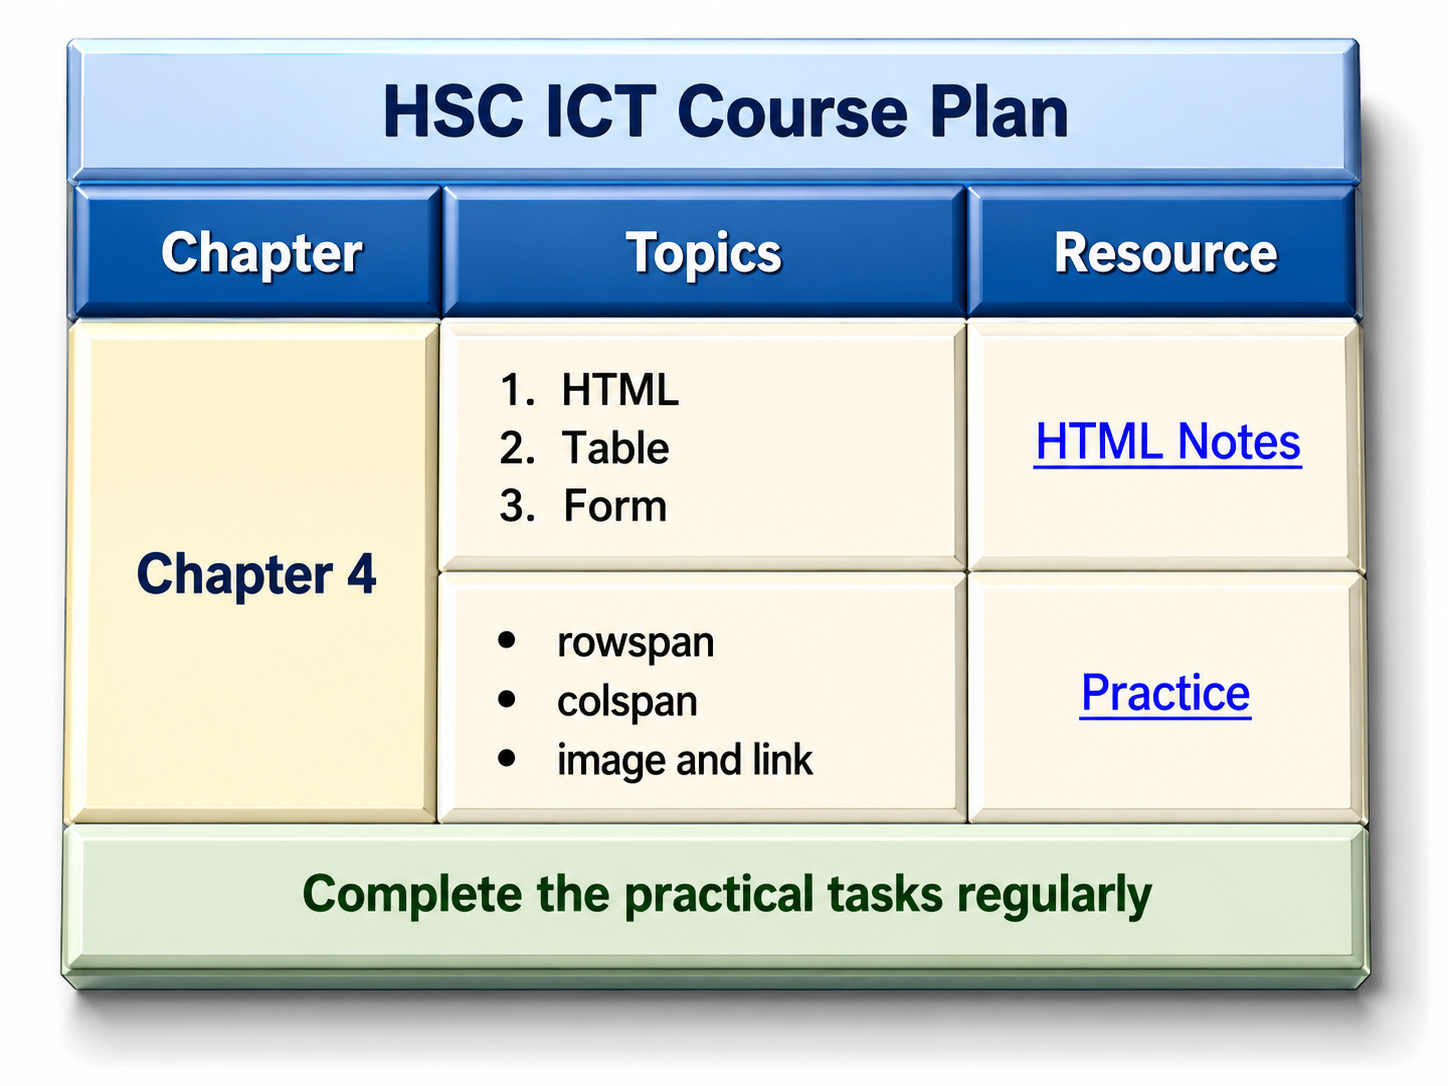
\includegraphics[width=0.95\linewidth,height=0.11\textheight,keepaspectratio]{chapters/Chapter04/topics/images/board_ex60_3d_course_plan_list_link.png}
}{
\fbox{\parbox{0.90\linewidth}{\centering\vspace{0.45cm}
\textbf{চিত্র}\\[3pt]
File: \texttt{chapters/Chapter04/topics/images/board\_ex60\_3d\_course\_plan\_list\_link.png}
\vspace{0.45cm}}}
}
\captionof{figure}{Course Plan Table with List, Link and Colspan}
\end{center}

\begin{keypointbox}{চিত্র ব্যাখ্যা}
একই table cell-এর ভিতরে ordered list ও unordered list রাখা হয়েছে, সাথে hyperlink ও colspan notice আছে।
\end{keypointbox}

\par\noindent{\color{purple!70!black}\bfseries\small কোড}\par\vspace{-4pt}
\begin{verbatim}
<!DOCTYPE html>
<html>
<head>
  <title>HTML Table Example</title>
</head>
<body>
<table border="1" cellspacing="0" cellpadding="6" align="center">
  <caption><b>HSC ICT Course Plan</b></caption>
  <tr>
    <th>Chapter</th>
    <th>Topics</th>
    <th>Resource</th>
  </tr>
  <tr>
    <td rowspan="2">Chapter 4</td>
    <td>
      <ol>
        <li>HTML</li>
        <li>Table</li>
        <li>Form</li>
      </ol>
    </td>
    <td><a href="html_notes.html">HTML Notes</a></td>
  </tr>
  <tr>
    <td>
      <ul>
        <li>rowspan</li>
        <li>colspan</li>
        <li>image and link</li>
      </ul>
    </td>
    <td><a href="practice.html">Practice</a></td>
  </tr>
  <tr>
    <td colspan="3" align="center">Complete the practical tasks regularly</td>
  </tr>
</table>
</body>
</html>
\end{verbatim}
\vspace{-6pt}

\begin{keypointbox}{Board technique}
প্রথমে মোট row ও column গুনবে। তারপর কোন cell horizontal merge হলে \texttt{colspan} এবং vertical merge হলে \texttt{rowspan} ব্যবহার করবে। image-এর জন্য \texttt{<img>} এবং link-এর জন্য \texttt{<a>} tag ব্যবহার করবে।
\end{keypointbox}


\subsubsection{Example 61: Library Book Table with Cover Image and Download Link}

\begin{center}
\IfFileExists{chapters/Chapter04/topics/images/board_ex61_3d_library_book_table.png}{
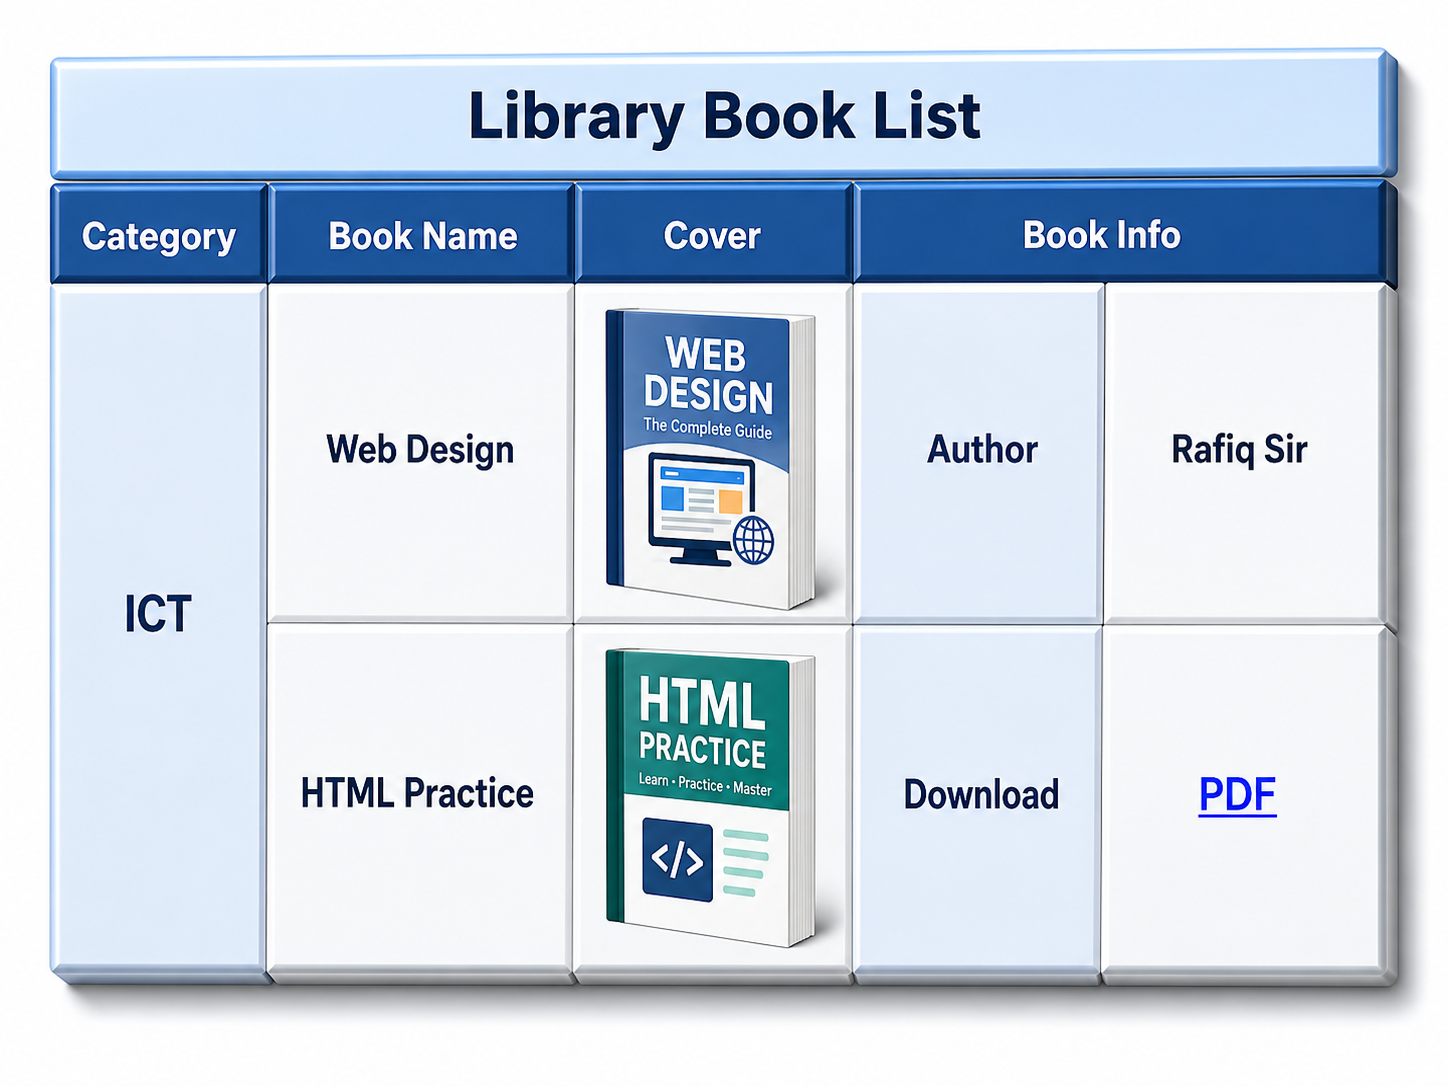
\includegraphics[width=0.95\linewidth,height=0.11\textheight,keepaspectratio]{chapters/Chapter04/topics/images/board_ex61_3d_library_book_table.png}
}{
\fbox{\parbox{0.90\linewidth}{\centering\vspace{0.45cm}
\textbf{চিত্র}\\[3pt]
File: \texttt{chapters/Chapter04/topics/images/board\_ex61\_3d\_library\_book\_table.png}
\vspace{0.45cm}}}
}
\captionof{figure}{Library Book Table with Cover Image and Download Link}
\end{center}

\begin{keypointbox}{চিত্র ব্যাখ্যা}
Category rowspan দিয়ে দুই বইকে একই category-তে দেখানো হয়েছে। Cover image ও PDF link দুই ধরনের content দেখানো হয়েছে।
\end{keypointbox}

\begin{keypointbox}{চিত্র দেখে code লেখার ধাপ}
প্রথমে figure-এর total row ও column গুনবে। এরপর কোন cell একাধিক column জুড়ে আছে তা দেখে \texttt{colspan} এবং কোন cell একাধিক row জুড়ে আছে তা দেখে \texttt{rowspan} বসাবে। তারপর image, link, list বা nested table থাকলে সংশ্লিষ্ট tag cell-এর ভিতরে লিখবে।
\end{keypointbox}

\par\noindent{\color{purple!70!black}\bfseries\small কোড}\par\vspace{-4pt}
\begin{verbatim}
<!DOCTYPE html>
<html>
<head>
  <title>HTML Table Example</title>
</head>
<body>
<table border="1" cellspacing="0" cellpadding="6" align="center">
  <caption><b>Library Book List</b></caption>
  <tr>
    <th>Category</th>
    <th>Book Name</th>
    <th>Cover</th>
    <th colspan="2">Book Info</th>
  </tr>
  <tr>
    <td rowspan="2">ICT</td>
    <td>Web Design</td>
    <td><img src="web_book.jpg" width="70" height="90" alt="Web Book"></td>
    <td>Author</td>
    <td>Rafiq Sir</td>
  </tr>
  <tr>
    <td>HTML Practice</td>
    <td><img src="html_book.jpg" width="70" height="90" alt="HTML Book"></td>
    <td>Download</td>
    <td><a href="html_practice.pdf">PDF</a></td>
  </tr>
</table>
</body>
</html>
\end{verbatim}
\vspace{-6pt}

\begin{keypointbox}{Board technique}
প্রথমে মোট row ও column গুনবে। তারপর কোন cell horizontal merge হলে \texttt{colspan} এবং vertical merge হলে \texttt{rowspan} ব্যবহার করবে। image-এর জন্য \texttt{<img>} এবং link-এর জন্য \texttt{<a>} tag ব্যবহার করবে।
\end{keypointbox}


\subsubsection{Example 62: Exam Routine with Date Rowspan and Subject Colspan}

\begin{center}
\IfFileExists{chapters/Chapter04/topics/images/board_ex62_3d_exam_routine_table.png}{
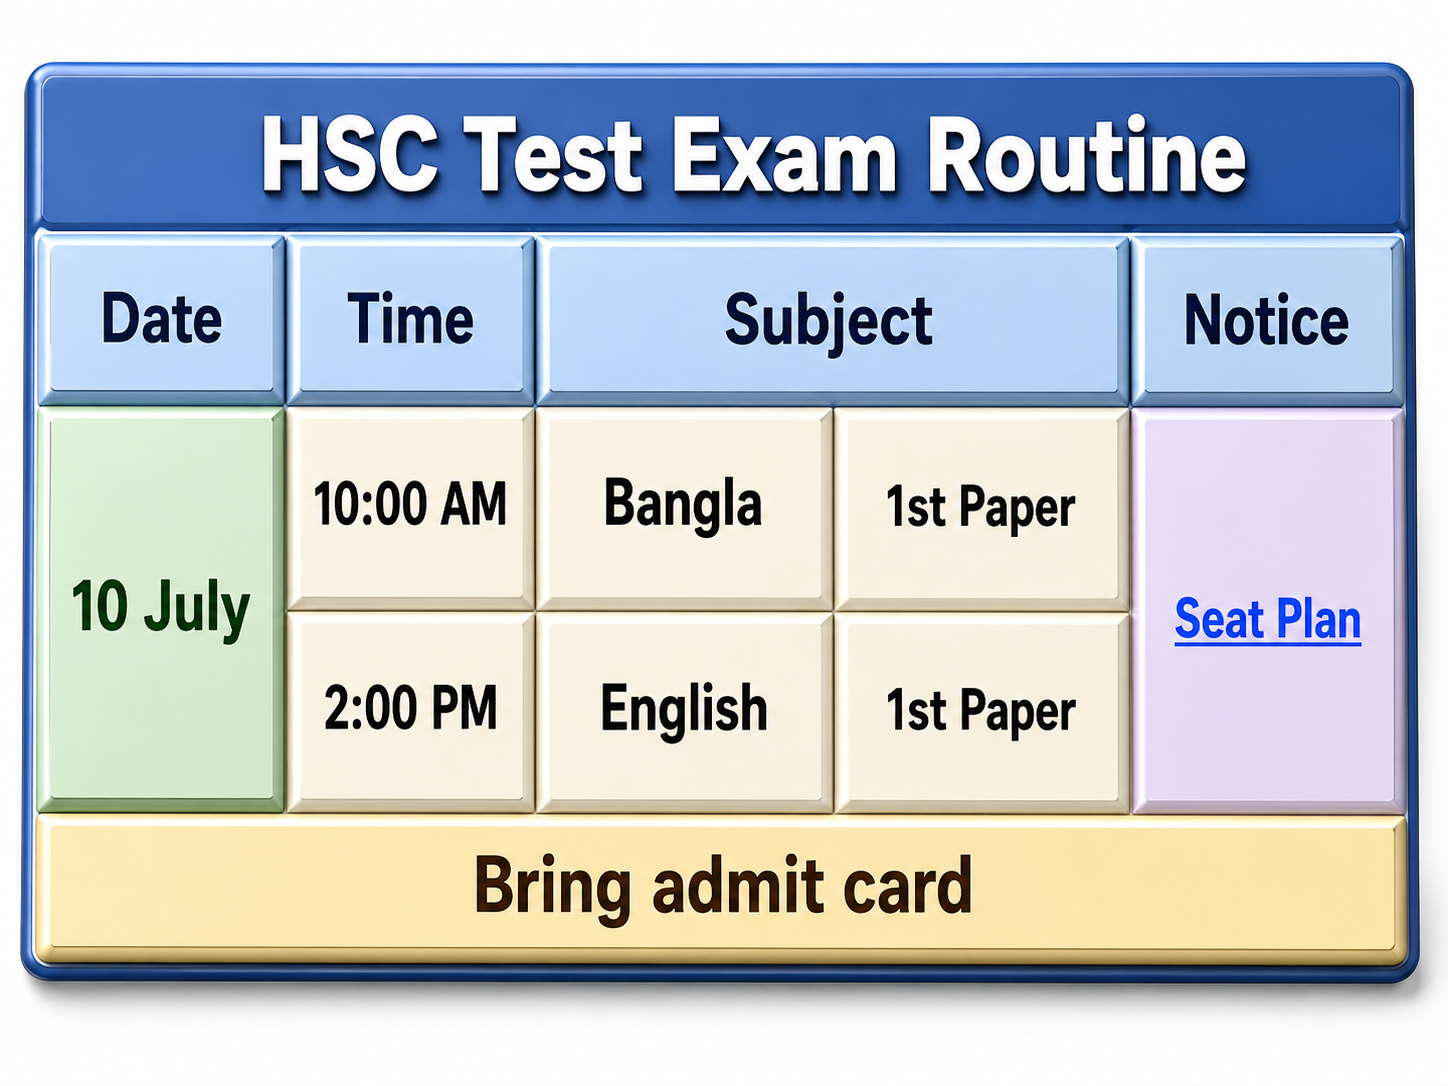
\includegraphics[width=0.95\linewidth,height=0.11\textheight,keepaspectratio]{chapters/Chapter04/topics/images/board_ex62_3d_exam_routine_table.png}
}{
\fbox{\parbox{0.90\linewidth}{\centering\vspace{0.45cm}
\textbf{চিত্র}\\[3pt]
File: \texttt{chapters/Chapter04/topics/images/board\_ex62\_3d\_exam\_routine\_table.png}
\vspace{0.45cm}}}
}
\captionof{figure}{Exam Routine with Date Rowspan and Subject Colspan}
\end{center}

\begin{keypointbox}{চিত্র ব্যাখ্যা}
একই তারিখের দুই exam দেখাতে Date এবং Notice cell-এ rowspan ব্যবহার করা হয়েছে। Subject heading দুই column জুড়ে আছে।
\end{keypointbox}

\par\noindent{\color{purple!70!black}\bfseries\small কোড}\par\vspace{-4pt}
\begin{verbatim}
<!DOCTYPE html>
<html>
<head>
  <title>HTML Table Example</title>
</head>
<body>
<table border="1" cellspacing="0" cellpadding="6" align="center">
  <caption><b>HSC Test Exam Routine</b></caption>
  <tr>
    <th>Date</th>
    <th>Time</th>
    <th colspan="2">Subject</th>
    <th>Notice</th>
  </tr>
  <tr>
    <td rowspan="2">10 July</td>
    <td>10:00 AM</td>
    <td>Bangla</td>
    <td>1st Paper</td>
    <td rowspan="2"><a href="seat_plan.html">Seat Plan</a></td>
  </tr>
  <tr>
    <td>2:00 PM</td>
    <td>English</td>
    <td>1st Paper</td>
  </tr>
  <tr>
    <td colspan="5" align="center">Bring admit card</td>
  </tr>
</table>
</body>
</html>
\end{verbatim}
\vspace{-6pt}

\begin{keypointbox}{Board technique}
প্রথমে মোট row ও column গুনবে। তারপর কোন cell horizontal merge হলে \texttt{colspan} এবং vertical merge হলে \texttt{rowspan} ব্যবহার করবে। image-এর জন্য \texttt{<img>} এবং link-এর জন্য \texttt{<a>} tag ব্যবহার করবে।
\end{keypointbox}


\subsubsection{Example 63: ICT Lab Inventory with Device Image and Manual Link}

\begin{center}
\IfFileExists{chapters/Chapter04/topics/images/board_ex63_3d_lab_inventory_table.png}{
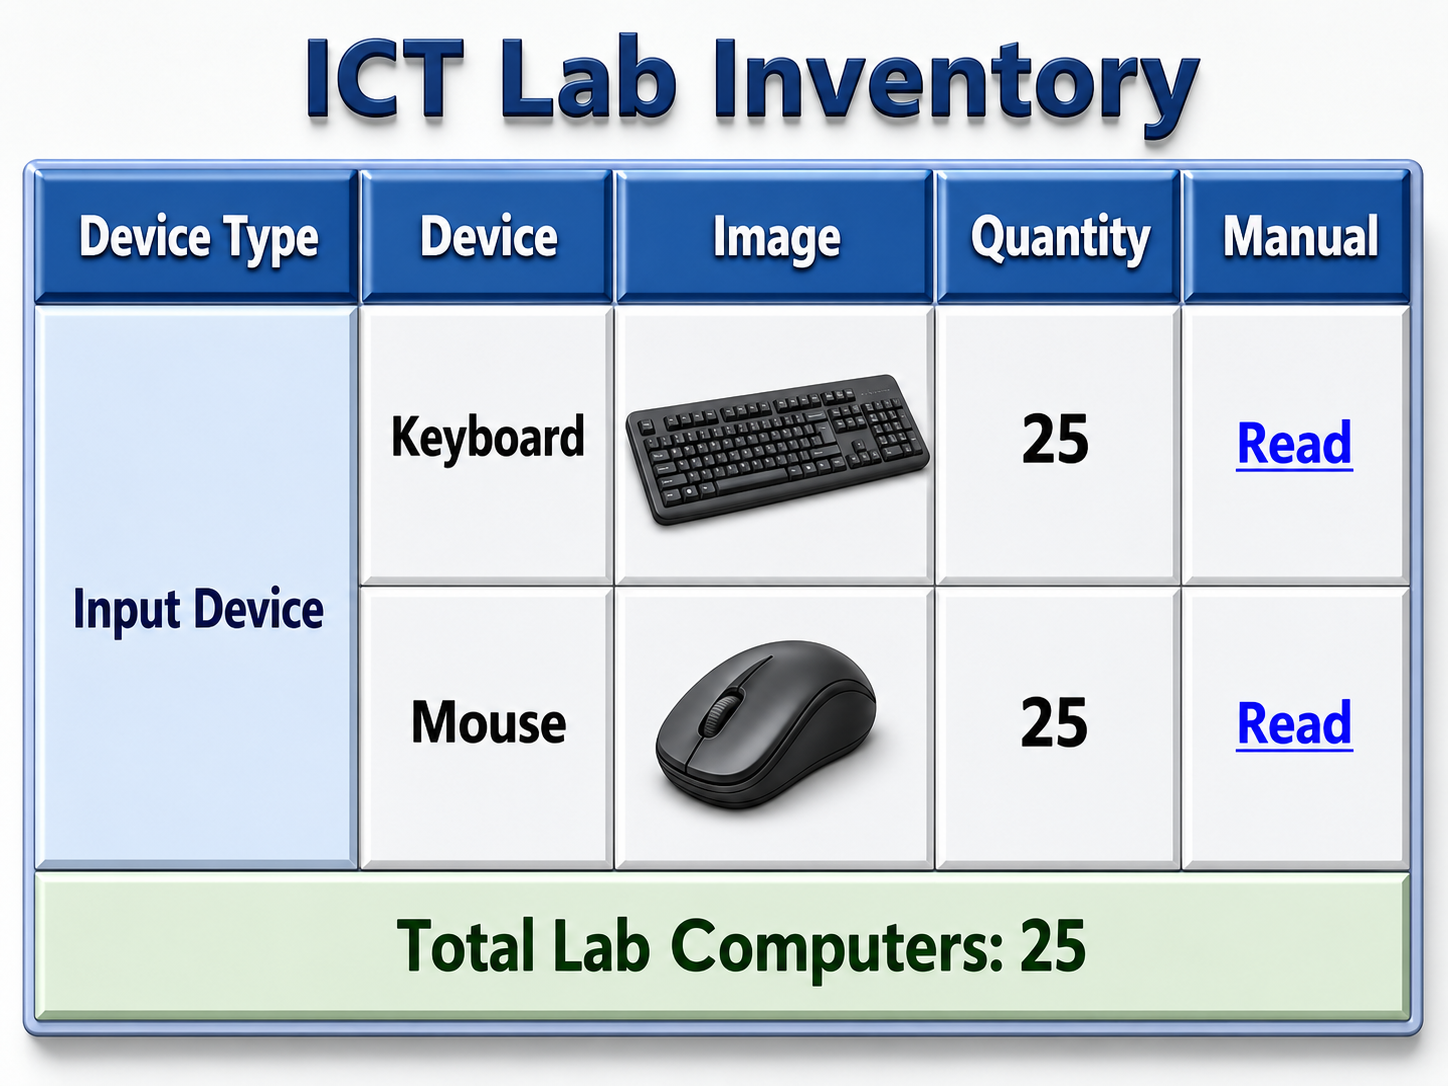
\includegraphics[width=0.95\linewidth,height=0.11\textheight,keepaspectratio]{chapters/Chapter04/topics/images/board_ex63_3d_lab_inventory_table.png}
}{
\fbox{\parbox{0.90\linewidth}{\centering\vspace{0.45cm}
\textbf{চিত্র}\\[3pt]
File: \texttt{chapters/Chapter04/topics/images/board\_ex63\_3d\_lab\_inventory\_table.png}
\vspace{0.45cm}}}
}
\captionof{figure}{ICT Lab Inventory with Device Image and Manual Link}
\end{center}

\begin{keypointbox}{চিত্র ব্যাখ্যা}
Device Type rowspan দিয়ে দুই input device group করা হয়েছে। প্রতিটি device-এর image ও manual link আছে।
\end{keypointbox}

\begin{keypointbox}{চিত্র দেখে code লেখার ধাপ}
প্রথমে figure-এর total row ও column গুনবে। এরপর কোন cell একাধিক column জুড়ে আছে তা দেখে \texttt{colspan} এবং কোন cell একাধিক row জুড়ে আছে তা দেখে \texttt{rowspan} বসাবে। তারপর image, link, list বা nested table থাকলে সংশ্লিষ্ট tag cell-এর ভিতরে লিখবে।
\end{keypointbox}

\par\noindent{\color{purple!70!black}\bfseries\small কোড}\par\vspace{-4pt}
\begin{verbatim}
<!DOCTYPE html>
<html>
<head>
  <title>HTML Table Example</title>
</head>
<body>
<table border="1" cellspacing="0" cellpadding="6" align="center">
  <caption><b>ICT Lab Inventory</b></caption>
  <tr>
    <th>Device Type</th>
    <th>Device</th>
    <th>Image</th>
    <th>Quantity</th>
    <th>Manual</th>
  </tr>
  <tr>
    <td rowspan="2">Input Device</td>
    <td>Keyboard</td>
    <td><img src="keyboard.jpg" width="80" height="50" alt="Keyboard"></td>
    <td>25</td>
    <td><a href="keyboard.html">Read</a></td>
  </tr>
  <tr>
    <td>Mouse</td>
    <td><img src="mouse.jpg" width="80" height="50" alt="Mouse"></td>
    <td>25</td>
    <td><a href="mouse.html">Read</a></td>
  </tr>
  <tr>
    <td colspan="5" align="center">Total Lab Computers: 25</td>
  </tr>
</table>
</body>
</html>
\end{verbatim}
\vspace{-6pt}

\begin{keypointbox}{Board technique}
প্রথমে মোট row ও column গুনবে। তারপর কোন cell horizontal merge হলে \texttt{colspan} এবং vertical merge হলে \texttt{rowspan} ব্যবহার করবে। image-এর জন্য \texttt{<img>} এবং link-এর জন্য \texttt{<a>} tag ব্যবহার করবে।
\end{keypointbox}


\subsubsection{Example 64: Restaurant Menu with Specials, Image, Link and Colspan}

\begin{center}
\IfFileExists{chapters/Chapter04/topics/images/board_ex64_3d_restaurant_menu_mixed.png}{
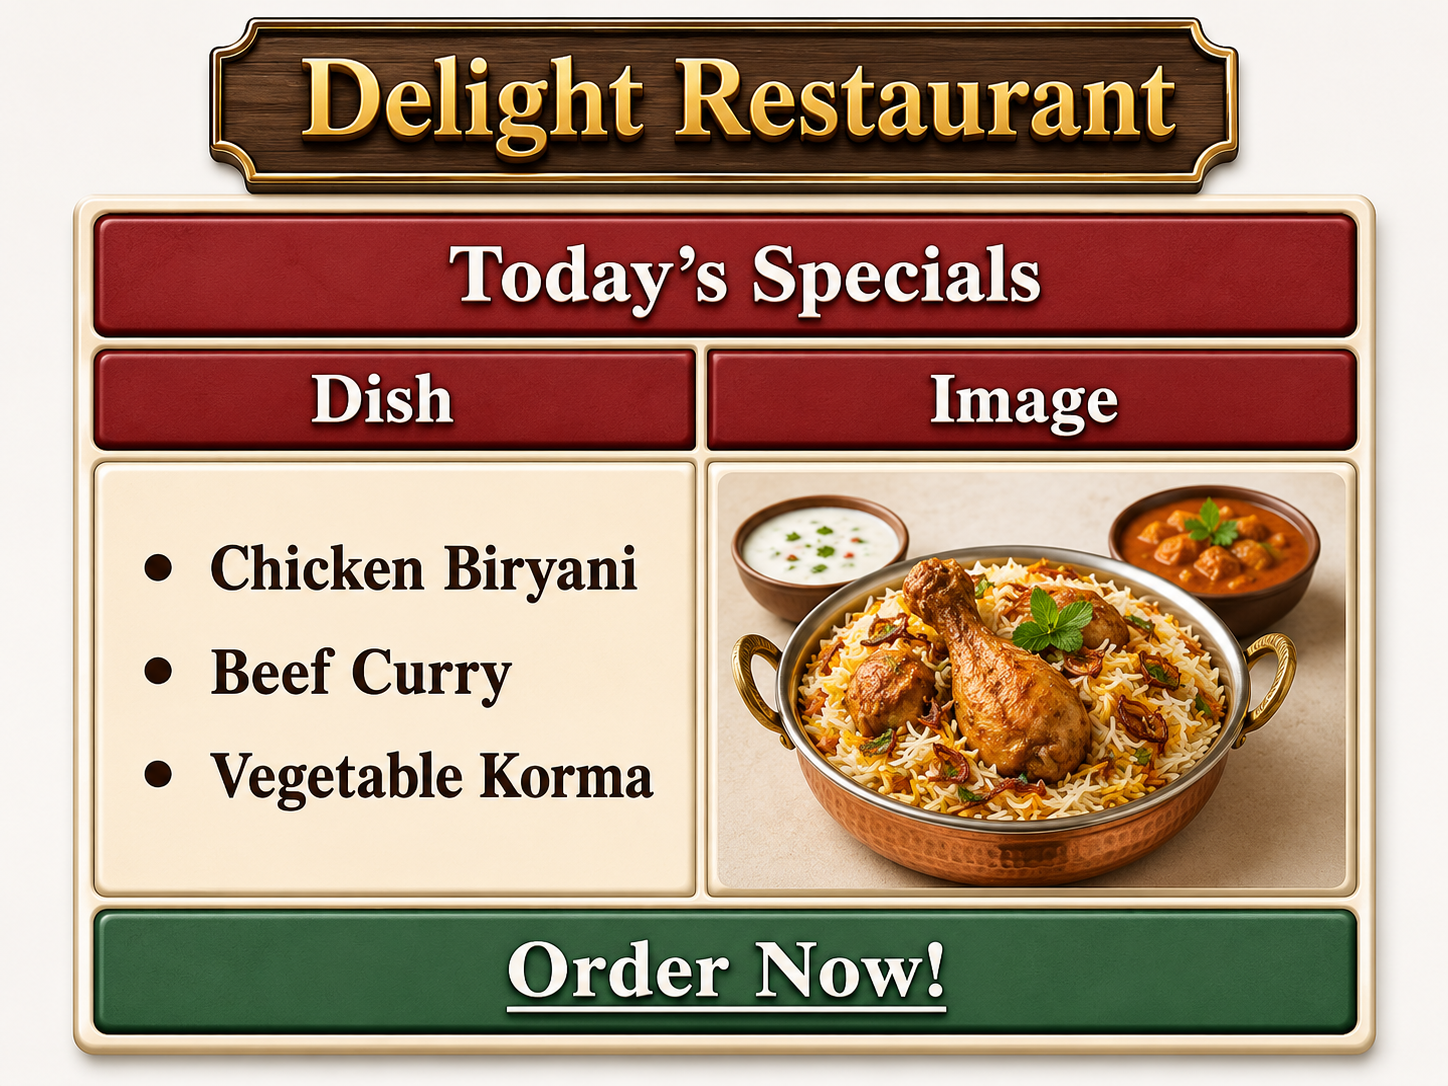
\includegraphics[width=0.95\linewidth,height=0.11\textheight,keepaspectratio]{chapters/Chapter04/topics/images/board_ex64_3d_restaurant_menu_mixed.png}
}{
\fbox{\parbox{0.90\linewidth}{\centering\vspace{0.45cm}
\textbf{চিত্র}\\[3pt]
File: \texttt{chapters/Chapter04/topics/images/board\_ex64\_3d\_restaurant\_menu\_mixed.png}
\vspace{0.45cm}}}
}
\captionof{figure}{Restaurant menu with specials, image and colspan}
\end{center}

\begin{keypointbox}{চিত্র ব্যাখ্যা}
চিত্রে Delight Restaurant heading, Today's Specials title row, Dish ও Image দুইটি column, item list, food image এবং নিচে full-width Order Now row আছে।
\end{keypointbox}

\begin{keypointbox}{চিত্র দেখে code লেখার ধাপ}
প্রথমে restaurant heading লিখবে। তারপর two-column table বানাবে। Today's Specials row এবং Order Now row দুই column জুড়ে থাকবে, তাই দুই জায়গায় \texttt{colspan="2"} ব্যবহার করবে। Dish cell-এ list/line break এবং Image cell-এ \texttt{<img>} tag বসাবে।
\end{keypointbox}

\par\noindent{\color{purple!70!black}\bfseries\small কোড}\par\vspace{-4pt}
\begin{verbatim}
<!DOCTYPE html>
<html>
<head>
  <title>HTML Table Example</title>
</head>
<body>
<h2 align="center">Delight Restaurant</h2>
<table border="1" cellspacing="0" cellpadding="8" align="center">
  <tr>
    <th colspan="2">Today's Specials</th>
  </tr>
  <tr>
    <th>Dish</th>
    <th>Image</th>
  </tr>
  <tr>
    <td>
      <ul>
        <li>Chicken Biryani</li>
        <li>Beef Curry</li>
        <li>Vegetable Korma</li>
      </ul>
    </td>
    <td><img src="food.jpg" width="100" height="80" alt="Food"></td>
  </tr>
  <tr>
    <td colspan="2" align="center"><a href="order.html">Order Now!</a></td>
  </tr>
</table>
</body>
</html>
\end{verbatim}
\vspace{-6pt}

\begin{keypointbox}{Board technique}
প্রথমে মোট row ও column গুনবে। তারপর কোন cell horizontal merge হলে \texttt{colspan} এবং vertical merge হলে \texttt{rowspan} ব্যবহার করবে। image-এর জন্য \texttt{<img>} এবং link-এর জন্য \texttt{<a>} tag ব্যবহার করবে।
\end{keypointbox}

\subsubsection{Example 65: Student Club Table with Rowspan and Image Icon}

\begin{center}
\IfFileExists{chapters/Chapter04/topics/images/board_ex65_3d_student_club_table.png}{
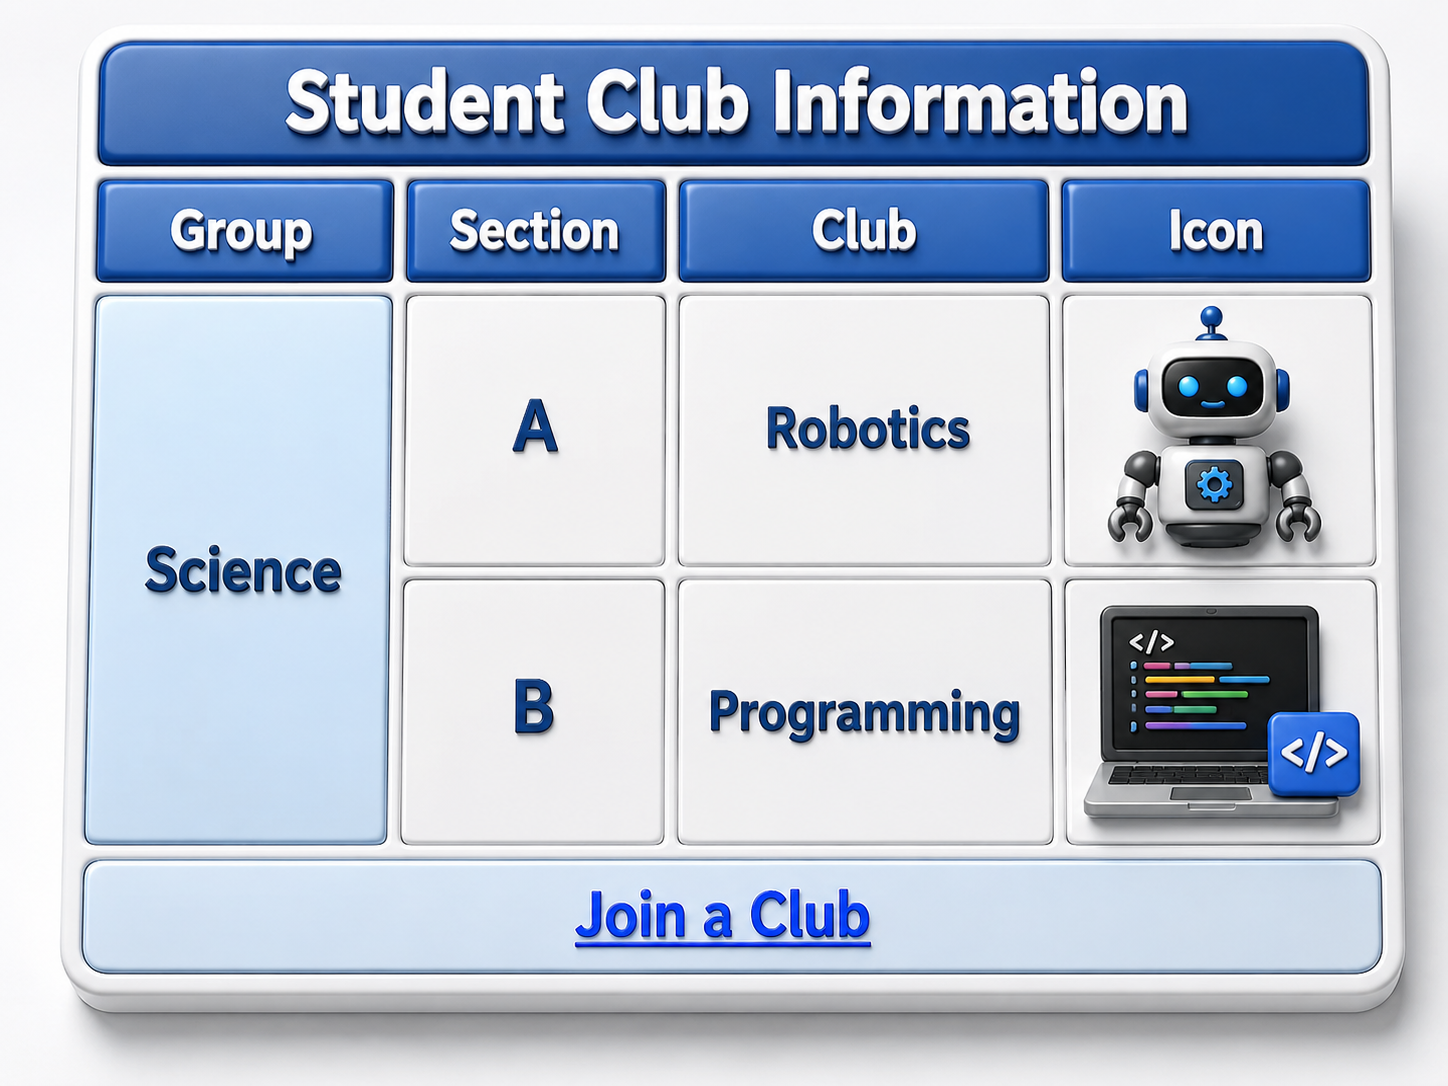
\includegraphics[width=0.95\linewidth,height=0.11\textheight,keepaspectratio]{chapters/Chapter04/topics/images/board_ex65_3d_student_club_table.png}
}{
\fbox{\parbox{0.90\linewidth}{\centering\vspace{0.45cm}
\textbf{চিত্র}\\[3pt]
File: \texttt{chapters/Chapter04/topics/images/board\_ex65\_3d\_student\_club\_table.png}
\vspace{0.45cm}}}
}
\captionof{figure}{Student Club Table with Rowspan and Image Icon}
\end{center}

\begin{keypointbox}{চিত্র ব্যাখ্যা}
Science group-এর দুই section দেখাতে rowspan, club icon দেখাতে image এবং join link দেখাতে colspan ব্যবহার করা হয়েছে।
\end{keypointbox}

\begin{keypointbox}{চিত্র দেখে code লেখার ধাপ}
প্রথমে figure-এর total row ও column গুনবে। এরপর কোন cell একাধিক column জুড়ে আছে তা দেখে \texttt{colspan} এবং কোন cell একাধিক row জুড়ে আছে তা দেখে \texttt{rowspan} বসাবে। তারপর image, link, list বা nested table থাকলে সংশ্লিষ্ট tag cell-এর ভিতরে লিখবে।
\end{keypointbox}

\par\noindent{\color{purple!70!black}\bfseries\small কোড}\par\vspace{-4pt}
\begin{verbatim}
<!DOCTYPE html>
<html>
<head>
  <title>HTML Table Example</title>
</head>
<body>
<table border="1" cellspacing="0" cellpadding="6" align="center">
  <caption><b>Student Club Information</b></caption>
  <tr>
    <th>Group</th>
    <th>Section</th>
    <th>Club</th>
    <th>Icon</th>
  </tr>
  <tr>
    <td rowspan="2">Science</td>
    <td>A</td>
    <td>Robotics</td>
    <td><img src="robot.png" width="50" height="50" alt="Robot"></td>
  </tr>
  <tr>
    <td>B</td>
    <td>Programming</td>
    <td><img src="code.png" width="50" height="50" alt="Code"></td>
  </tr>
  <tr>
    <td colspan="4" align="center"><a href="club.html">Join a Club</a></td>
  </tr>
</table>
</body>
</html>
\end{verbatim}
\vspace{-6pt}

\begin{keypointbox}{Board technique}
প্রথমে মোট row ও column গুনবে। তারপর কোন cell horizontal merge হলে \texttt{colspan} এবং vertical merge হলে \texttt{rowspan} ব্যবহার করবে। image-এর জন্য \texttt{<img>} এবং link-এর জন্য \texttt{<a>} tag ব্যবহার করবে।
\end{keypointbox}


\subsubsection{Example 66: Blood Donor Table with Contact Colspan}

\begin{center}
\IfFileExists{chapters/Chapter04/topics/images/board_ex66_3d_blood_donor_contact.png}{
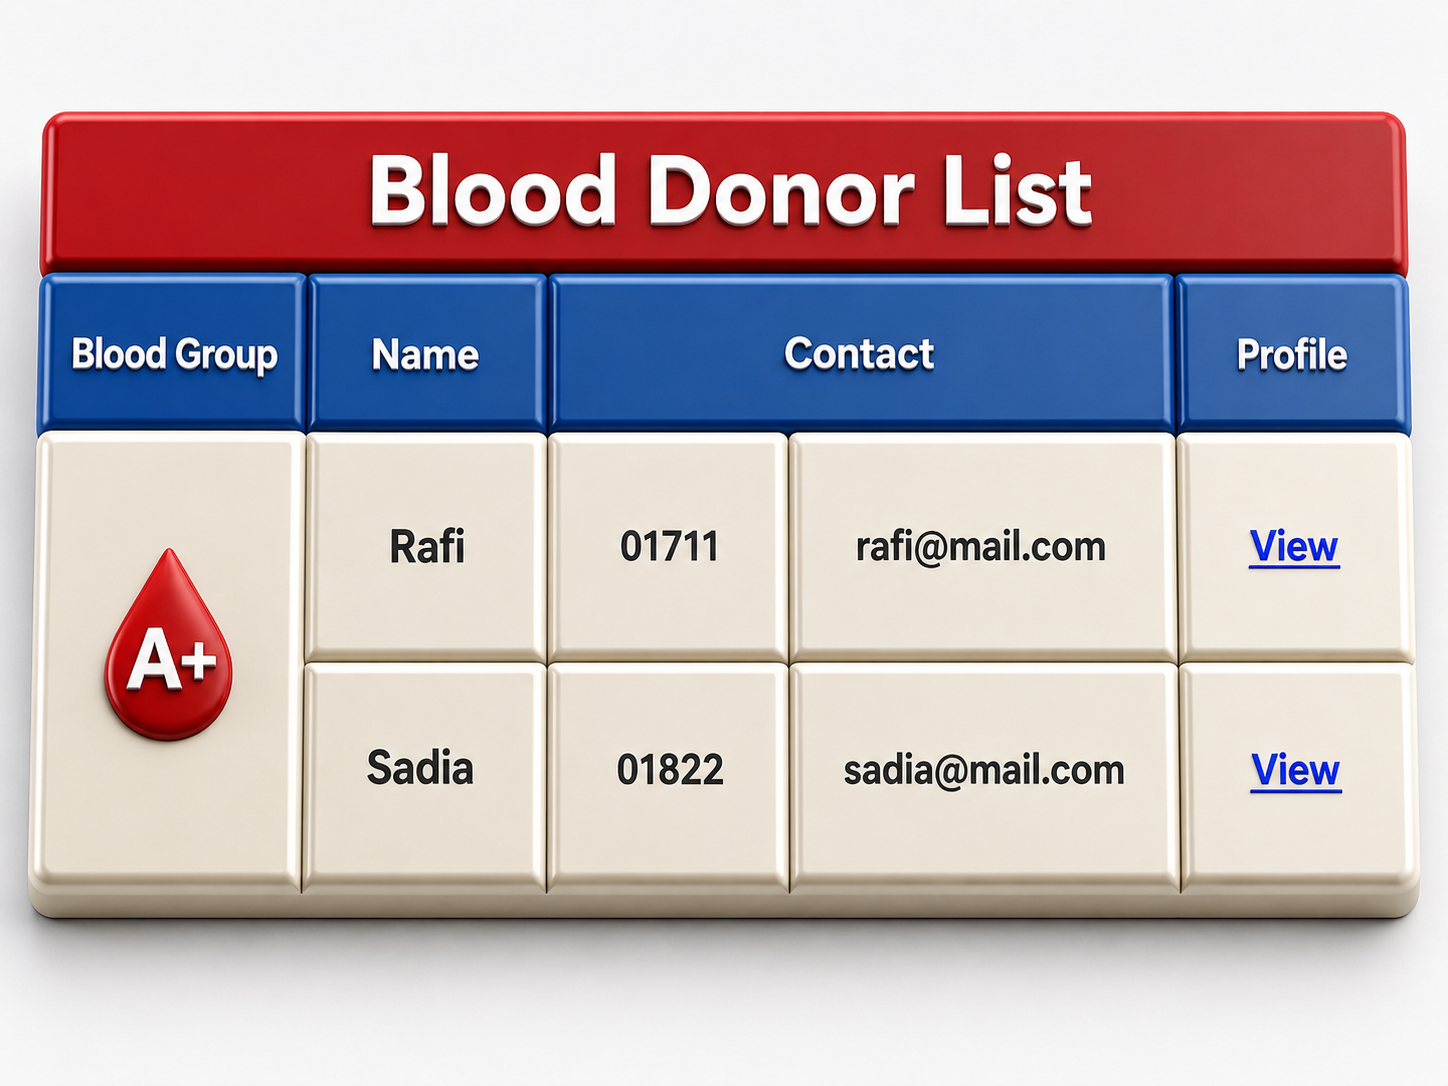
\includegraphics[width=0.95\linewidth,height=0.11\textheight,keepaspectratio]{chapters/Chapter04/topics/images/board_ex66_3d_blood_donor_contact.png}
}{
\fbox{\parbox{0.90\linewidth}{\centering\vspace{0.45cm}
\textbf{চিত্র}\\[3pt]
File: \texttt{chapters/Chapter04/topics/images/board\_ex66\_3d\_blood\_donor\_contact.png}
\vspace{0.45cm}}}
}
\captionof{figure}{Blood Donor Table with Contact Colspan}
\end{center}

\begin{keypointbox}{চিত্র ব্যাখ্যা}
Contact heading দুই column জুড়ে আছে এবং A+ blood group দুই donor-এর জন্য rowspan করা হয়েছে।
\end{keypointbox}

\par\noindent{\color{purple!70!black}\bfseries\small কোড}\par\vspace{-4pt}
\begin{verbatim}
<!DOCTYPE html>
<html>
<head>
  <title>HTML Table Example</title>
</head>
<body>
<table border="1" cellspacing="0" cellpadding="6" align="center">
  <caption><b>Blood Donor List</b></caption>
  <tr>
    <th>Blood Group</th>
    <th>Name</th>
    <th colspan="2">Contact</th>
    <th>Profile</th>
  </tr>
  <tr>
    <td rowspan="2">A+</td>
    <td>Rafi</td>
    <td>01711</td>
    <td>rafi@mail.com</td>
    <td><a href="rafi.html">View</a></td>
  </tr>
  <tr>
    <td>Sadia</td>
    <td>01822</td>
    <td>sadia@mail.com</td>
    <td><a href="sadia.html">View</a></td>
  </tr>
</table>
</body>
</html>
\end{verbatim}
\vspace{-6pt}

\begin{keypointbox}{Board technique}
প্রথমে মোট row ও column গুনবে। তারপর কোন cell horizontal merge হলে \texttt{colspan} এবং vertical merge হলে \texttt{rowspan} ব্যবহার করবে। image-এর জন্য \texttt{<img>} এবং link-এর জন্য \texttt{<a>} tag ব্যবহার করবে।
\end{keypointbox}


\subsubsection{Example 67: Scholarship Table with Logo, Link and Merged Eligibility}

\begin{center}
\IfFileExists{chapters/Chapter04/topics/images/board_ex67_3d_scholarship_table.png}{
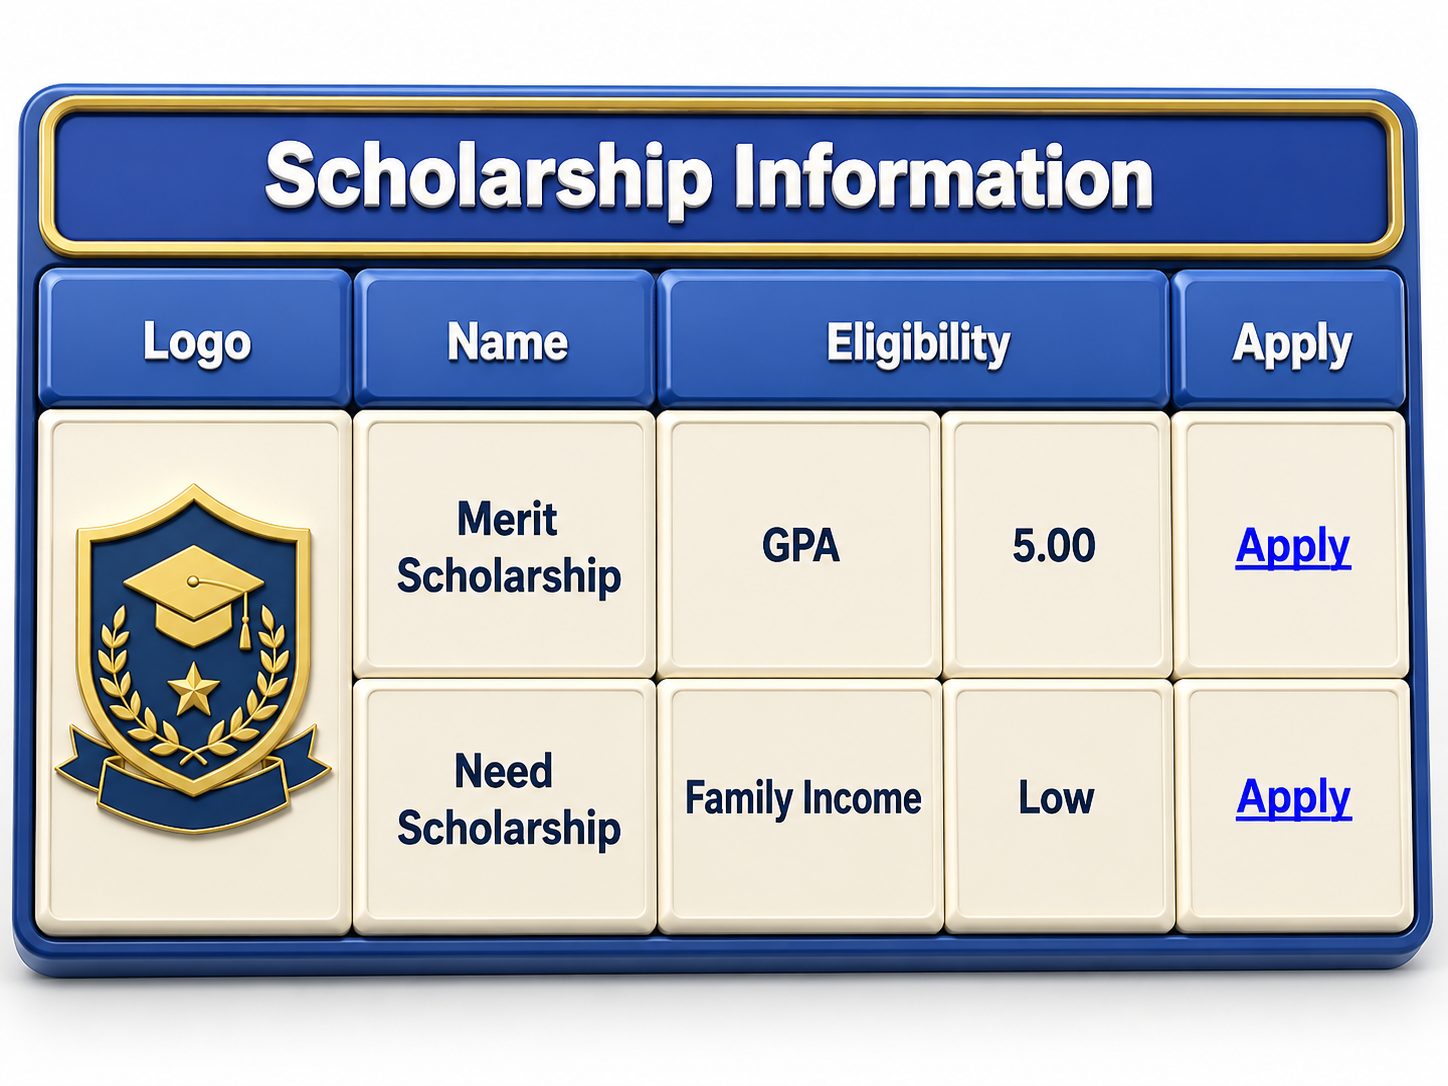
\includegraphics[width=0.95\linewidth,height=0.11\textheight,keepaspectratio]{chapters/Chapter04/topics/images/board_ex67_3d_scholarship_table.png}
}{
\fbox{\parbox{0.90\linewidth}{\centering\vspace{0.45cm}
\textbf{চিত্র}\\[3pt]
File: \texttt{chapters/Chapter04/topics/images/board\_ex67\_3d\_scholarship\_table.png}
\vspace{0.45cm}}}
}
\captionof{figure}{Scholarship Table with Logo, Link and Merged Eligibility}
\end{center}

\begin{keypointbox}{চিত্র ব্যাখ্যা}
Logo দুই scholarship row জুড়ে আছে; Eligibility heading দুই column জুড়ে আছে।
\end{keypointbox}

\begin{keypointbox}{চিত্র দেখে code লেখার ধাপ}
প্রথমে figure-এর total row ও column গুনবে। এরপর কোন cell একাধিক column জুড়ে আছে তা দেখে \texttt{colspan} এবং কোন cell একাধিক row জুড়ে আছে তা দেখে \texttt{rowspan} বসাবে। তারপর image, link, list বা nested table থাকলে সংশ্লিষ্ট tag cell-এর ভিতরে লিখবে।
\end{keypointbox}

\par\noindent{\color{purple!70!black}\bfseries\small কোড}\par\vspace{-4pt}
\begin{verbatim}
<!DOCTYPE html>
<html>
<head>
  <title>HTML Table Example</title>
</head>
<body>
<table border="1" cellspacing="0" cellpadding="6" align="center">
  <caption><b>Scholarship Information</b></caption>
  <tr>
    <th>Logo</th>
    <th>Name</th>
    <th colspan="2">Eligibility</th>
    <th>Apply</th>
  </tr>
  <tr>
    <td rowspan="2"><img src="scholarship.png" width="70" height="70" alt="Scholarship"></td>
    <td>Merit Scholarship</td>
    <td>GPA</td>
    <td>5.00</td>
    <td><a href="merit.html">Apply</a></td>
  </tr>
  <tr>
    <td>Need Scholarship</td>
    <td>Family Income</td>
    <td>Low</td>
    <td><a href="need.html">Apply</a></td>
  </tr>
</table>
</body>
</html>
\end{verbatim}
\vspace{-6pt}

\begin{keypointbox}{Board technique}
প্রথমে মোট row ও column গুনবে। তারপর কোন cell horizontal merge হলে \texttt{colspan} এবং vertical merge হলে \texttt{rowspan} ব্যবহার করবে। image-এর জন্য \texttt{<img>} এবং link-এর জন্য \texttt{<a>} tag ব্যবহার করবে।
\end{keypointbox}


\subsubsection{Example 68: Website Layout Table with Header, Sidebar, Image and Footer}

\begin{center}
\IfFileExists{chapters/Chapter04/topics/images/board_ex68_3d_webpage_layout_table.png}{
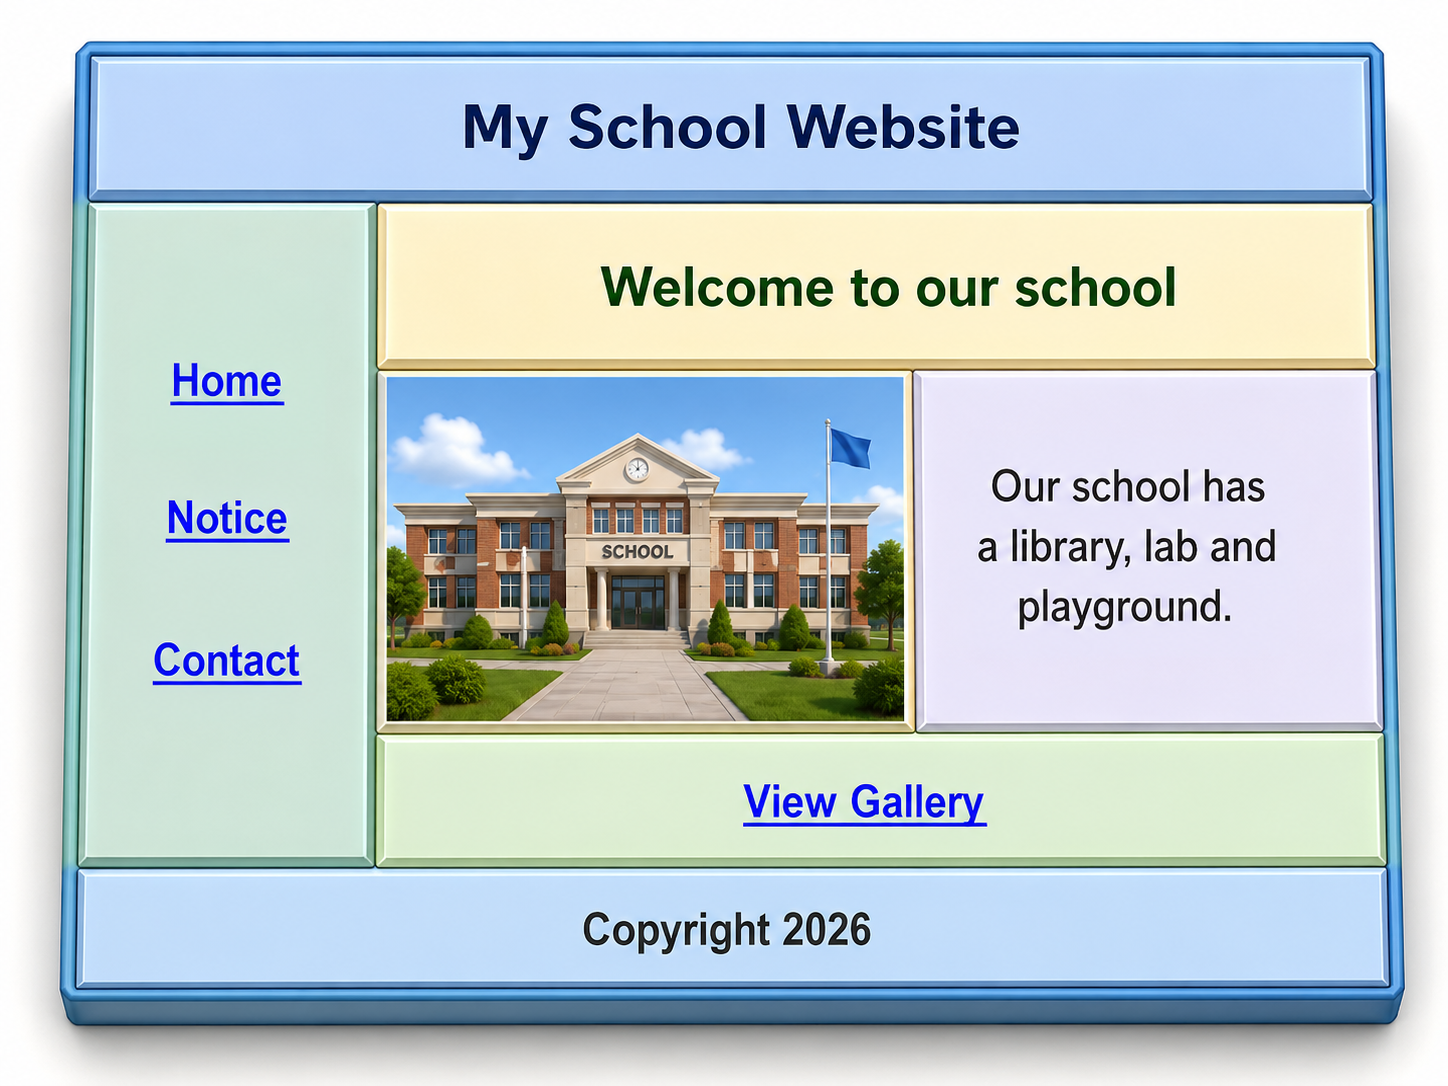
\includegraphics[width=0.95\linewidth,height=0.11\textheight,keepaspectratio]{chapters/Chapter04/topics/images/board_ex68_3d_webpage_layout_table.png}
}{
\fbox{\parbox{0.90\linewidth}{\centering\vspace{0.45cm}
\textbf{চিত্র}\\[3pt]
File: \texttt{chapters/Chapter04/topics/images/board\_ex68\_3d\_webpage\_layout\_table.png}
\vspace{0.45cm}}}
}
\captionof{figure}{Website Layout Table with Header, Sidebar, Image and Footer}
\end{center}

\begin{keypointbox}{চিত্র ব্যাখ্যা}
এটি webpage layout style table। Header ও footer colspan, sidebar rowspan, image এবং multiple links ব্যবহার করা হয়েছে।
\end{keypointbox}

\par\noindent{\color{purple!70!black}\bfseries\small কোড}\par\vspace{-4pt}
\begin{verbatim}
<!DOCTYPE html>
<html>
<head>
  <title>HTML Table Example</title>
</head>
<body>
<table border="1" cellspacing="0" cellpadding="8" align="center" width="600">
  <tr>
    <th colspan="3">My School Website</th>
  </tr>
  <tr>
    <td rowspan="3">
      <a href="home.html">Home</a><br>
      <a href="notice.html">Notice</a><br>
      <a href="contact.html">Contact</a>
    </td>
    <td colspan="2" align="center">Welcome to our school</td>
  </tr>
  <tr>
    <td><img src="school.jpg" width="150" height="90" alt="School"></td>
    <td>Our school has a library, lab and playground.</td>
  </tr>
  <tr>
    <td colspan="2" align="center"><a href="gallery.html">View Gallery</a></td>
  </tr>
  <tr>
    <td colspan="3" align="center">Copyright 2026</td>
  </tr>
</table>
</body>
</html>
\end{verbatim}
\vspace{-6pt}

\begin{keypointbox}{Board technique}
প্রথমে মোট row ও column গুনবে। তারপর কোন cell horizontal merge হলে \texttt{colspan} এবং vertical merge হলে \texttt{rowspan} ব্যবহার করবে। image-এর জন্য \texttt{<img>} এবং link-এর জন্য \texttt{<a>} tag ব্যবহার করবে।
\end{keypointbox}


\subsubsection{Example 69: College Contact Card with Nested Table, Image and Link}

\begin{center}
\IfFileExists{chapters/Chapter04/topics/images/board_ex69_3d_college_contact_nested.png}{
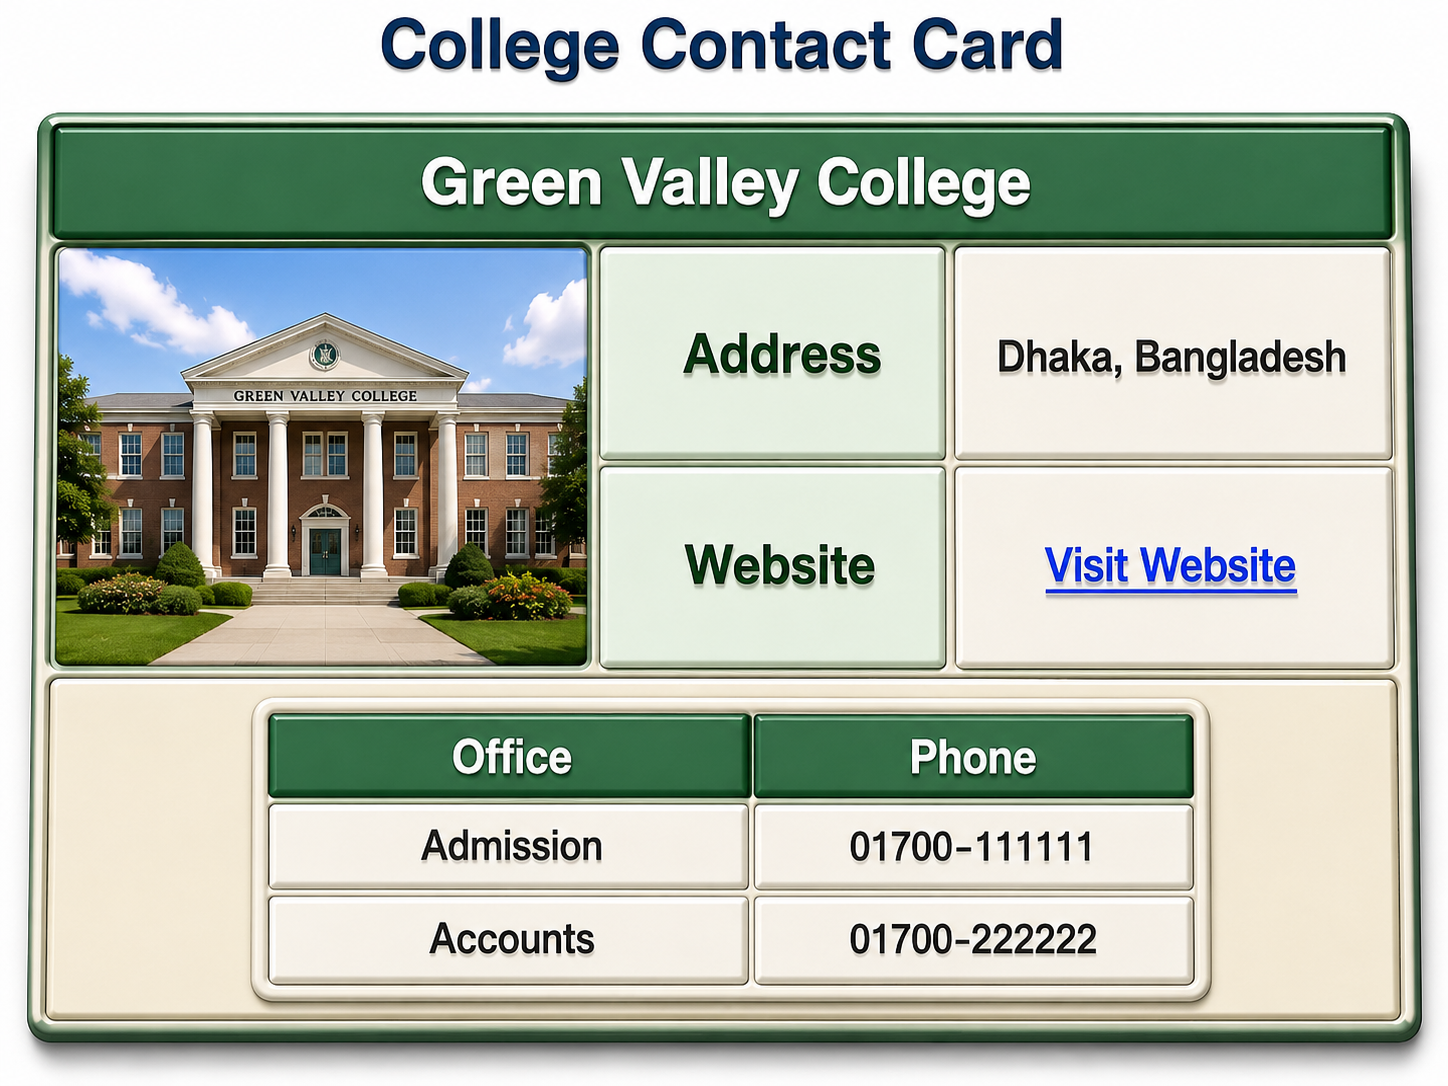
\includegraphics[width=0.95\linewidth,height=0.11\textheight,keepaspectratio]{chapters/Chapter04/topics/images/board_ex69_3d_college_contact_nested.png}
}{
\fbox{\parbox{0.90\linewidth}{\centering\vspace{0.45cm}
\textbf{চিত্র}\\[3pt]
File: \texttt{chapters/Chapter04/topics/images/board\_ex69\_3d\_college\_contact\_nested.png}
\vspace{0.45cm}}}
}
\captionof{figure}{College Contact Card with Nested Table, Image and Link}
\end{center}

\begin{keypointbox}{চিত্র ব্যাখ্যা}
এখানে outer table-এর ভিতরে nested table আছে। College image rowspan, title colspan এবং website hyperlink ব্যবহার করা হয়েছে।
\end{keypointbox}

\begin{keypointbox}{চিত্র দেখে code লেখার ধাপ}
প্রথমে figure-এর total row ও column গুনবে। এরপর কোন cell একাধিক column জুড়ে আছে তা দেখে \texttt{colspan} এবং কোন cell একাধিক row জুড়ে আছে তা দেখে \texttt{rowspan} বসাবে। তারপর image, link, list বা nested table থাকলে সংশ্লিষ্ট tag cell-এর ভিতরে লিখবে।
\end{keypointbox}

\par\noindent{\color{purple!70!black}\bfseries\small কোড}\par\vspace{-4pt}
\begin{verbatim}
<!DOCTYPE html>
<html>
<head>
  <title>HTML Table Example</title>
</head>
<body>
<table border="1" cellspacing="0" cellpadding="6" align="center">
  <caption><b>College Contact Card</b></caption>
  <tr>
    <th colspan="3">Green Valley College</th>
  </tr>
  <tr>
    <td rowspan="2"><img src="college.jpg" width="120" height="80" alt="College"></td>
    <td>Address</td>
    <td>Dhaka, Bangladesh</td>
  </tr>
  <tr>
    <td>Website</td>
    <td><a href="https://example.com">Visit Website</a></td>
  </tr>
  <tr>
    <td colspan="3">
      <table border="1" cellspacing="0" cellpadding="4" align="center">
        <tr>
          <th>Office</th>
          <th>Phone</th>
        </tr>
        <tr>
          <td>Admission</td>
          <td>01700-111111</td>
        </tr>
        <tr>
          <td>Accounts</td>
          <td>01700-222222</td>
        </tr>
      </table>
    </td>
  </tr>
</table>
</body>
</html>
\end{verbatim}
\vspace{-6pt}

\begin{keypointbox}{Board technique}
প্রথমে মোট row ও column গুনবে। তারপর কোন cell horizontal merge হলে \texttt{colspan} এবং vertical merge হলে \texttt{rowspan} ব্যবহার করবে। image-এর জন্য \texttt{<img>} এবং link-এর জন্য \texttt{<a>} tag ব্যবহার করবে।
\end{keypointbox}


\end{multicols}

\begin{recapbox}
এই ১৫টি mixed table practice-এ \texttt{rowspan}, \texttt{colspan}, image, hyperlink, list, nested table, caption, alignment এবং width—সব ধরনের গুরুত্বপূর্ণ HSC ICT table concept একসাথে cover করা হয়েছে। Exam-এ চিত্র দেখে code লেখার আগে structure analysis করাই সবচেয়ে গুরুত্বপূর্ণ।
\end{recapbox}

\subsection{চিত্র দেখে Table লেখার Final Checklist}

Board practical বা CQ-তে table-এর চিত্র দেওয়া থাকলে নিচের checklist ব্যবহার করলে ভুল কম হয়। এটি simple table, merged table, image/link/list-সহ table এবং nested table--সব ধরনের প্রশ্নে কাজে লাগে।

\begin{enumerate}
\item Table-এর নাম বা caption আছে কি না দেখবে।
\item Header row আছে কি না দেখবে।
\item Visible column সংখ্যা গুনবে।
\item Visible row সংখ্যা গুনবে।
\item Merged cell থাকলে আগে \texttt{rowspan} না \texttt{colspan} তা ঠিক করবে।
\item যে cell-এ image আছে সেখানে \texttt{<img>} এবং \texttt{alt} লিখবে।
\item যে cell-এ link আছে সেখানে \texttt{<a href="">} ব্যবহার করবে।
\item যে cell-এ list আছে সেখানে \texttt{<ol>} বা \texttt{<ul>} ব্যবহার করবে।
\item Nested table থাকলে inner table আলাদা indentation দিয়ে লিখবে।
\item শেষে সব \texttt{<table>}, \texttt{<tr>}, \texttt{<td>} tag close হয়েছে কি না মিলিয়ে দেখবে।
\end{enumerate}

\begin{keypointbox}{শেষ মুহূর্তের পরীক্ষা}
Code লেখা শেষ হলে প্রতিটি row আলাদা করে দেখবে: row-এর মোট column count figure-এর সাথে মিলছে কি না। \texttt{colspan="2"} মানে ওই cell দুই column-এর জায়গা নিয়েছে, তাই সেই row-তে একটি cell কম থাকবে। \texttt{rowspan="2"} মানে পরের row-তে ওই column-এর জন্য নতুন cell লিখতে হবে না।
\end{keypointbox}

\subsection{Board/Exam Focus}

\begin{boardbox}{বেশি গুরুত্বপূর্ণ}
\begin{itemize}
\item \texttt{<table>} tag table তৈরির জন্য ব্যবহৃত হয়।
\item \texttt{<tr>} row তৈরি করে।
\item \texttt{<th>} heading cell তৈরি করে।
\item \texttt{<td>} data cell তৈরি করে।
\item \texttt{<caption>} table-এর title দেয়।
\item \texttt{border} table border দেখায়।
\item \texttt{cellspacing} cell-এর মাঝের gap নির্ধারণ করে।
\item \texttt{cellpadding} cell-এর ভিতরের gap নির্ধারণ করে।
\item \texttt{rowspan} cell-কে vertical direction-এ merge করে।
\item \texttt{colspan} cell-কে horizontal direction-এ merge করে।
\item table-এর ভিতরে link, image, list এবং nested table ব্যবহার করা যায়।
\item চিত্র দেখে HTML table code লিখতে পারা খুব গুরুত্বপূর্ণ।
\end{itemize}
\end{boardbox}

\subsection{Exam-style Short Answer}

\begin{enumerate}
\item \textbf{HTML table কী?}\\
উত্তর: HTML document-এ তথ্যকে সারি ও কলাম আকারে প্রদর্শনের জন্য যে কাঠামো ব্যবহার করা হয়, তাকে HTML table বলে। Table তৈরির জন্য \texttt{<table>} tag ব্যবহার করা হয়।

\item \textbf{\texttt{<tr>} tag-এর কাজ কী?}\\
উত্তর: HTML table-এর একটি row বা সারি তৈরি করার জন্য \texttt{<tr>} tag ব্যবহার করা হয়।

\item \textbf{\texttt{<th>} ও \texttt{<td>} tag-এর পার্থক্য লেখ।}\\
উত্তর: \texttt{<th>} tag table-এর heading cell তৈরি করে এবং browser সাধারণত এর text bold ও center aligned করে দেখায়। অন্যদিকে \texttt{<td>} tag table-এর সাধারণ data cell তৈরি করে।

\item \textbf{\texttt{border} attribute-এর কাজ কী?}\\
উত্তর: HTML table-এর চারপাশে এবং cell-এর চারপাশে border বা রেখা প্রদর্শনের জন্য \texttt{border} attribute ব্যবহার করা হয়।

\item \textbf{\texttt{cellspacing} ও \texttt{cellpadding}-এর পার্থক্য লেখ।}\\
উত্তর: \texttt{cellspacing} cell থেকে cell-এর মাঝের gap নির্ধারণ করে। অন্যদিকে \texttt{cellpadding} cell-এর content এবং cell border-এর মাঝের ভিতরের gap নির্ধারণ করে।

\item \textbf{\texttt{rowspan} ও \texttt{colspan}-এর পার্থক্য লেখ।}\\
উত্তর: \texttt{rowspan} একটি cell-কে একাধিক row জুড়ে বিস্তৃত করে। \texttt{colspan} একটি cell-কে একাধিক column জুড়ে বিস্তৃত করে।

\item \textbf{Table-এর ভিতরে image বসানোর code লেখ।}\\
উত্তর: \texttt{<td><img src="photo.jpg" width="100" height="80" alt="Photo"></td>}

\item \textbf{Nested table কী?}\\
উত্তর: একটি table-এর কোনো cell-এর ভিতরে আরেকটি table তৈরি করলে তাকে nested table বলে।
\end{enumerate}

\subsection{Practice MCQ}

\begin{enumerate}
\item HTML-এ table তৈরির tag কোনটি?\\
ক) \texttt{<tr>} \quad খ) \texttt{<td>} \quad গ) \texttt{<table>} \quad ঘ) \texttt{<th>}

\item Table row তৈরি করতে কোন tag ব্যবহার হয়?\\
ক) \texttt{<td>} \quad খ) \texttt{<tr>} \quad গ) \texttt{<th>} \quad ঘ) \texttt{<caption>}

\item Table heading cell তৈরির tag কোনটি?\\
ক) \texttt{<td>} \quad খ) \texttt{<tr>} \quad গ) \texttt{<th>} \quad ঘ) \texttt{<br>}

\item Table data cell তৈরির tag কোনটি?\\
ক) \texttt{<td>} \quad খ) \texttt{<tr>} \quad গ) \texttt{<table>} \quad ঘ) \texttt{<hr>}

\item Table-এর border দেখাতে কোন attribute ব্যবহার করা হয়?\\
ক) \texttt{src} \quad খ) \texttt{href} \quad গ) \texttt{border} \quad ঘ) \texttt{target}

\item \texttt{cellpadding="5"} এর অর্থ কী?\\
ক) cell-এর ভিতরে content ও border-এর মাঝে 5 pixel space\\
খ) দুই cell-এর মাঝে 5 meter space\\
গ) table-এর height 5\\
ঘ) table-এর row সংখ্যা 5

\item \texttt{cellspacing} কোথায় space তৈরি করে?\\
ক) content ও border-এর ভিতরে \quad খ) cell ও cell-এর মাঝে \quad গ) image-এর ভিতরে \quad ঘ) hyperlink-এর পরে

\item দুইটি column merge করতে কোন attribute ব্যবহার হয়?\\
ক) \texttt{rowspan} \quad খ) \texttt{colspan} \quad গ) \texttt{cellpadding} \quad ঘ) \texttt{bgcolor}

\item দুইটি row merge করতে কোন attribute ব্যবহার হয়?\\
ক) \texttt{rowspan} \quad খ) \texttt{colspan} \quad গ) \texttt{align} \quad ঘ) \texttt{src}

\item Table-এর title দিতে কোন tag ব্যবহার হয়?\\
ক) \texttt{<title>} \quad খ) \texttt{<caption>} \quad গ) \texttt{<thead>} \quad ঘ) \texttt{<link>}

\item Image কোন tag দিয়ে table cell-এর ভিতরে বসানো যায়?\\
ক) \texttt{<a>} \quad খ) \texttt{<img>} \quad গ) \texttt{<ol>} \quad ঘ) \texttt{<tr>}

\item একটি table-এর cell-এর ভিতরে আরেকটি table বসালে তাকে কী বলে?\\
ক) outer table \quad খ) nested table \quad গ) image table \quad ঘ) child table
\end{enumerate}

\begin{boardbox}{MCQ Answer Key}
১-গ, ২-খ, ৩-গ, ৪-ক, ৫-গ, ৬-ক, ৭-খ, ৮-খ, ৯-ক, ১০-খ, ১১-খ, ১২-খ
\end{boardbox}

\subsection{CQ Practice}

\begin{practicebox}
\textbf{উদ্দীপক:} একটি webpage-এ Result Sheet table দেখাতে হবে। Table-এ border থাকবে, cell-এর ভিতরে ৫ pixel space থাকবে এবং cellগুলোর মাঝের gap থাকবে না। Table-এর প্রথম row-তে \texttt{Result Sheet} লেখা থাকবে এবং সেটি তিনটি column জুড়ে থাকবে।

\textbf{প্রশ্ন}\\
ক. HTML table কী?\\
খ. \texttt{<th>} ও \texttt{<td>} tag-এর কাজ লেখ।\\
গ. উদ্দীপকের জন্য HTML code লেখ।\\
ঘ. \texttt{border}, \texttt{cellspacing}, \texttt{cellpadding} ও \texttt{colspan} attribute-এর ব্যবহার বিশ্লেষণ কর।
\end{practicebox}

\subsubsection{গ. কোড}

\begin{examplebox}{কোড}
\begin{verbatim}
<!DOCTYPE html>
<html>
<head>
  <title>Result Table</title>
</head>
<body>
  <table border="1" cellspacing="0" cellpadding="5">
    <tr>
      <th colspan="3">Result Sheet</th>
    </tr>
    <tr>
      <th>Roll</th>
      <th>Name</th>
      <th>GPA</th>
    </tr>
    <tr>
      <td>101</td>
      <td>Rafi</td>
      <td>5.00</td>
    </tr>
    <tr>
      <td>102</td>
      <td>Sakib</td>
      <td>4.75</td>
    </tr>
  </table>
</body>
</html>
\end{verbatim}
\end{examplebox}

\subsubsection{ঘ. বিশ্লেষণ}

\texttt{border="1"} table ও cell-এর চারপাশে border দেখায়। \texttt{cellspacing="0"} cellগুলোর মাঝের gap দূর করে। \texttt{cellpadding="5"} cell-এর ভিতরে content ও border-এর মাঝে ৫ pixel space তৈরি করে, ফলে table পড়তে সহজ হয়। \texttt{colspan="3"} প্রথম heading cell-কে তিনটি column জুড়ে বিস্তৃত করে, তাই \texttt{Result Sheet} title পুরো table-এর উপর দেখা যায়।

\subsection{Common Mistake}

\begin{mistakebox}{সাধারণ ভুল}
\begin{itemize}
\item \texttt{<table>} tag close না করা।
\item \texttt{<tr>} ছাড়া সরাসরি \texttt{<td>} লেখা।
\item heading cell-এ \texttt{<td>} ব্যবহার করা, যেখানে \texttt{<th>} ভালো।
\item \texttt{<td>}-এর spelling ভুল করে \texttt{<tb>} লেখা।
\item \texttt{cellpadding} ও \texttt{cellspacing} গুলিয়ে ফেলা।
\item \texttt{rowspan} ও \texttt{colspan} উল্টো ব্যবহার করা।
\item border না দিলে table-এর রেখা দেখা যাবে না--এটা ভুলে যাওয়া।
\item table row ও column সংখ্যা figure-এর সাথে না মেলানো।
\item \texttt{<caption>} ভুল জায়গায় লেখা। Caption সাধারণত \texttt{<table>} tag-এর ভিতরে, প্রথম row-এর আগে লেখা হয়।
\item table-এর ভিতরে image/link/list লিখতে syntax ভুল করা।
\item image tag-এ \texttt{src} ভুল দেওয়া বা image file একই folder-এ না রাখা।
\item nested table-এর closing tag ঠিকমতো না দেওয়া।
\end{itemize}
\end{mistakebox}

\subsection{১ মিনিটে রিভিশন}

\begin{recapbox}
Table তৈরি হয় row ও column দিয়ে। \texttt{<table>} পুরো table তৈরি করে, \texttt{<tr>} table row তৈরি করে, \texttt{<th>} heading cell তৈরি করে এবং \texttt{<td>} data cell তৈরি করে। \texttt{border} table border দেখায়, \texttt{cellspacing} cell-এর মাঝের gap নিয়ন্ত্রণ করে এবং \texttt{cellpadding} cell-এর ভিতরের gap নিয়ন্ত্রণ করে। \texttt{<caption>} table-এর title দেয়। \texttt{rowspan} vertical merge এবং \texttt{colspan} horizontal merge করে। Table cell-এর ভিতরে text, link, image, list ও nested table রাখা যায়। HSC CQ-তে table চিত্র দেখে code লেখা খুব গুরুত্বপূর্ণ।
\end{recapbox}











% Density revision 2026-10-04: answers below questions; compact related content.
% Topic 15: Rowspan and Colspan
\section{সারণির ঘর একত্র করা: rowspan ও colspan}

% Composition pass 2026-10-04
ফলের সারণিতে একটি শিরোনাম তিন কলামের ওপর এবং একটি বিষয় দুই সারির পাশে দেখাতে হবে।

\chFourMotivation{একাধিক মূল ঘরের স্থানজুড়ে একই তথ্য $\rightarrow$ colspan/rowspan $\rightarrow$ বিস্তৃত ঘরের দখল করা স্থান গোনা $\rightarrow$ ফল ও রুটিনের মিলিত শিরোনাম।}


\begin{learningbox}
এই অংশ শেষে শিক্ষার্থী পারবে:
\begin{itemize}
\item HTML সারণির ঘর একত্র করার ধারণা ব্যাখ্যা করতে।
\item \texttt{colspan} অ্যাট্রিবিউট ব্যবহার করে ঘরকে একাধিক কলামজুড়ে দেখাতে।
\item \texttt{rowspan} অ্যাট্রিবিউট ব্যবহার করে ঘরকে একাধিক সারিজুড়ে দেখাতে।
\item চিত্র দেখে \texttt{rowspan} ও \texttt{colspan} নির্ধারণ করতে।
\item একত্র করা ঘরের জন্য অতিরিক্ত \texttt{<td>} বা \texttt{<th>} না লেখার নিয়ম বুঝতে।
\end{itemize}
\end{learningbox}



একটি পরীক্ষার ফলের সারণিতে Roll, Name ও GPA তিনটি কলাম আছে। উপরে Result Sheet শিরোনামটি তিন কলামের মাঝ বরাবর দেখাতে আলাদা তিনটি ঘরে একই কথা লেখার প্রয়োজন নেই; একটি ঘরকে তিন কলামজুড়ে বিস্তৃত করলেই হয়। আবার একজনের দুটি ফোন নম্বর থাকলে Phone পরিচিতিটি দুই সারিজুড়ে একবার দেখানো যায়। এই অংশে \texttt{colspan} ও \texttt{rowspan} দিয়ে ঘরের বিস্তার এবং মূল ছকের স্থান গণনা শেখা হবে।

\subsection{ঘর একত্র করা (Cell Merge)}

\begin{definitionbox}{}
HTML সারণিতে একাধিক সারি বা কলামের স্থানজুড়ে একটি ঘর বিস্তৃত করে দেখানোকে \textbf{ঘর একত্র করা} বলে। এর জন্য \texttt{rowspan} ও \texttt{colspan} অ্যাট্রিবিউট ব্যবহার করা হয়।
\end{definitionbox}

ঘর একত্র করলে ছকের বিন্যাস বদলায়। আলাদা ঘরের লেখা স্বয়ংক্রিয়ভাবে একসঙ্গে যুক্ত হয় না। বিস্তৃত ঘরে কী লেখা থাকবে এবং ঘরটি কত সারি বা কলাম দখল করবে, তা কোডে নির্ধারণ করতে হয়।

\begin{examplebox}{সহজ উদাহরণ}
\begin{center}
\begin{tabular}{|c|c|c|}
\hline
\multicolumn{3}{|c|}{\textbf{Result Sheet}} \\
\hline
\textbf{Roll} & \textbf{Name} & \textbf{GPA} \\
\hline
\end{tabular}
\end{center}
এখানে \textbf{Result Sheet} ঘরটি ৩টি কলামজুড়ে আছে। তাই HTML কোডে \texttt{colspan="3"} ব্যবহার করতে হবে।
\end{examplebox}

\subsection{\texttt{colspan} দিয়ে কলামজুড়ে ঘর}

\texttt{colspan} একটি ঘর কতটি কলামজুড়ে থাকবে, তা নির্ধারণ করে। নিচের উদাহরণে Math ও ICT একই Subject শিরোনামের অধীনে আছে।

\texttt{colspan} নামটি Column Span অর্থাৎ কলামজুড়ে বিস্তার বোঝায়। এটি সাধারণত \texttt{<th>} বা \texttt{<td>} ট্যাগের ভেতরে লেখা হয়।

% Split revision: code and its explanation share one row.
\par\noindent
\begin{minipage}[t]{.54\linewidth}\vspace{0pt}\small
\subsubsection{লেখার রূপ}

\textbf{\color{chFourTeal}কোড}\par
\begin{verbatim}
<th colspan="number">Heading</th>
<td colspan="number">Data</td>
\end{verbatim}
\par\smallskip
\end{minipage}\hfill
\begin{minipage}[t]{.42\linewidth}\vspace{0pt}\small
\subsubsection{উদাহরণ}

\textbf{\color{chFourTeal}কোড}\par
\begin{verbatim}
<th colspan="2">Subject</th>
\end{verbatim}
\par\smallskip


এর অর্থ: \textbf{Subject} ঘরটি ২টি কলামজুড়ে থাকবে।
\end{minipage}\par
\subsection{কলামের উদাহরণ: বিষয়ের সারণি}

% Split revision: code and its explanation share one row.
\par\noindent
\begin{minipage}[t]{.60\linewidth}\vspace{0pt}\small
\textbf{\color{chFourTeal}কোড}\par
\begin{verbatim}
<!DOCTYPE html><html>
<head><title>Colspan Example</title></head>
<body><table border="1">
  <tr><th>Name</th><th colspan="2">Subject</th></tr>
  <tr><td>Kabir</td><td>Math</td><td>ICT</td></tr>
</table></body></html>
\end{verbatim}
\par\smallskip
\end{minipage}\hfill
\begin{minipage}[t]{.36\linewidth}\vspace{0pt}\small
\textbf{\color{chFourTeal}ফলের ধারণা}\par
\begin{center}
\begin{tabular}{|c|c|c|}
\hline
\textbf{Name} & \multicolumn{2}{c|}{\textbf{Subject}} \\
\hline
Kabir & Math & ICT \\
\hline
\end{tabular}
\end{center}
এখানে \textbf{Subject} শিরোনাম দুইটি কলাম--Math ও ICT--এর উপর বসেছে। তাই \texttt{Subject} ঘরে \texttt{colspan="2"} ব্যবহার হবে।
\par\smallskip
\end{minipage}\par


\begin{boardbox}{পরীক্ষায় মনে রাখবে}
একটি শিরোনাম যদি দুইটি কলামের উপর বসে, তাহলে \texttt{colspan="2"} লিখতে হয়। তিনটি কলাম হলে \texttt{colspan="3"} লিখতে হয়।
\end{boardbox}

\subsection{\texttt{rowspan} দিয়ে সারিজুড়ে ঘর}

\texttt{rowspan} একটি ঘর কতটি সারিজুড়ে থাকবে, তা নির্ধারণ করে। নিচের উদাহরণে Phone ঘরের পাশে দুই সারিতে দুটি নম্বর আছে।

\texttt{rowspan} নামটি Row Span অর্থাৎ সারিজুড়ে বিস্তার বোঝায়। এটি \texttt{<th>} অথবা \texttt{<td>} ট্যাগে ব্যবহার করা যায়।

% Split revision: code and its explanation share one row.
\par\noindent
\begin{minipage}[t]{.54\linewidth}\vspace{0pt}\small
\subsubsection{লেখার রূপ}

\textbf{\color{chFourTeal}কোড}\par
\begin{verbatim}
<th rowspan="number">Heading</th>
<td rowspan="number">Data</td>
\end{verbatim}
\par\smallskip
\end{minipage}\hfill
\begin{minipage}[t]{.42\linewidth}\vspace{0pt}\small
\subsubsection{উদাহরণ}

\textbf{\color{chFourTeal}কোড}\par
\begin{verbatim}
<th rowspan="2">Phone</th>
\end{verbatim}
\par\smallskip


এর অর্থ: \textbf{Phone} ঘরটি ২টি সারিজুড়ে থাকবে।
\end{minipage}\par
\subsection{সারির উদাহরণ: ফোন নম্বরের সারণি}

% Split revision: code and its explanation share one row.
\par\noindent
\begin{minipage}[t]{.50\linewidth}\vspace{0pt}\small
\textbf{\color{chFourTeal}কোড}\par
\begin{verbatim}
<table border="1">
  <tr>
    <th>Name</th>
    <td>Kabir</td>
  </tr>
  <tr>
    <th rowspan="2">Phone</th>
    <td>8942318</td>
  </tr>
  <tr>
    <td>1750181</td>
  </tr>
</table>
\end{verbatim}
\par\smallskip
\end{minipage}\hfill
\begin{minipage}[t]{.46\linewidth}\vspace{0pt}\small
\textbf{\color{chFourTeal}ফলের ধারণা}\par
\begin{center}
\begin{tabular}{|c|c|}
\hline
\textbf{Name} & Kabir \\
\hline
\raisebox{-.5\normalbaselineskip}[0pt][0pt]{\textbf{Phone}} & 8942318 \\
\cline{2-2}
 & 1750181 \\
\hline
\end{tabular}
\end{center}
এখানে \textbf{Phone} ঘরটি দুইটি ফোন নম্বরের পাশে দুইটি সারিজুড়ে আছে। তাই \texttt{rowspan="2"} ব্যবহার হবে।
\par\smallskip
\end{minipage}\par


% Original applied explanation; see Chapter04/SOURCES.md.
\subsubsection{রুটিনের ছক থেকে বিস্তৃত ঘর গণনা}
রুটিনে একটি ল্যাব ক্লাস দুই সময়ের ঘর দখল করলে \texttt{colspan="2"} ব্যবহার করা যায়। একটি বিভাগ-নাম তিনটি বিষয়ের সারি ধরে থাকলে \texttt{rowspan="3"} উপযোগী। বিস্তৃত ঘর যত স্থান দখল করে, ওই স্থানে আর নতুন ঘর লিখবে না।

কোড লেখার আগে কাগজে সারি-কলামের ছক আঁকবে। ওপরের সারি থেকে নেমে আগের rowspan-এর দখল করা স্থান চিহ্নিত করবে; তারপর অবশিষ্ট স্থানে নতুন \texttt{td}/\texttt{th} বসাবে। এইভাবে পুরো ছকের প্রস্থ একই থাকে এবং বাড়তি ঘর তৈরির ভুল ধরা যায়।


\subsection{rowspan ও colspan-এর পার্থক্য}

\begin{center}
\footnotesize
\begin{tabular}{|p{0.20\textwidth}|p{0.32\textwidth}|p{0.32\textwidth}|}
\hline
\textbf{বিষয়} & \textbf{\texttt{colspan}} & \textbf{\texttt{rowspan}} \\
\hline
কাজ & ঘরকে একাধিক কলামজুড়ে বিস্তৃত করে & ঘরকে একাধিক সারিজুড়ে বিস্তৃত করে \\
\hline
দিক & আড়াআড়ি & লম্বালম্বি \\
\hline
ব্যবহার & শিরোনাম কয়েকটি কলামের ওপর বসাতে & একটি পরিচিতি কয়েকটি সারির পাশে বসাতে \\
\hline
উদাহরণ & \texttt{<th colspan="3">Result</th>} & \texttt{<td rowspan="2">ICT</td>} \\
\hline
মনে রাখার উপায় & কলামজুড়ে বিস্তার & সারিজুড়ে বিস্তার \\
\hline
\end{tabular}
\end{center}

\subsection{অ্যাট্রিবিউট দুটি কোথায় লেখা হয়?}

\texttt{rowspan} ও \texttt{colspan} সাধারণত \texttt{<td>} অথবা \texttt{<th>} ট্যাগের ভেতরে লেখা হয়।

\begin{examplebox}{কোড}
\begin{verbatim}
<th colspan="3">Result Sheet</th>
<td rowspan="2">ICT</td>
\end{verbatim}
\end{examplebox}

\begin{keypointbox}{মূল নিয়ম}
\texttt{colspan}-এর জন্য ধনাত্মক পূর্ণসংখ্যা দিতে হয়; যেমন \texttt{colspan="3"} মানে তিনটি কলাম। এখানকার \texttt{rowspan="2"} মানে দুইটি সারি। বিশেষ ক্ষেত্রে \texttt{rowspan="0"} বর্তমান সারি-দলের অবশিষ্ট সব সারি বোঝায়; সাধারণ চিত্রভিত্তিক অনুশীলনে যতটি সারি বিস্তৃত হয়েছে, সেই সংখ্যা লিখবে।
\end{keypointbox}

\subsection{ফলের সারণির শিরোনামে colspan}

% Split revision: code and its explanation share one row.
\par\noindent
\begin{minipage}[t]{.54\linewidth}\vspace{0pt}\small
\textbf{\color{chFourTeal}কোড}\par
\begin{verbatim}
<table border="1" cellspacing="0" cellpadding="5">
  <tr>
    <th colspan="3">Result Sheet</th>
  </tr>
  <tr>
    <th>Roll</th><th>Name</th><th>GPA</th>
  </tr>
  <tr>
    <td>101</td><td>Rafi</td><td>5.00</td>
  </tr>
</table>
\end{verbatim}
\par\smallskip
\end{minipage}\hfill
\begin{minipage}[t]{.42\linewidth}\vspace{0pt}\small
\textbf{\color{chFourTeal}ফলের ধারণা}\par
\begin{center}
\begin{tabular}{|c|c|c|}
\hline
\multicolumn{3}{|c|}{\textbf{Result Sheet}} \\
\hline
\textbf{Roll} & \textbf{Name} & \textbf{GPA} \\
\hline
101 & Rafi & 5.00 \\
\hline
\end{tabular}
\end{center}
\par\smallskip
\end{minipage}\par


\begin{keypointbox}{ব্যাখ্যা}
সারণিতে মোট ৩টি কলাম আছে: Roll, Name, GPA। Result Sheet শিরোনাম পুরো ৩টি কলামজুড়ে থাকবে। তাই \texttt{<th colspan="3">Result Sheet</th>} লেখা হয়েছে।
\end{keypointbox}

\subsection{বিষয়ভিত্তিক নম্বরের সারণিতে rowspan}

% Split revision: code and its explanation share one row.
\par\noindent
\begin{minipage}[t]{.54\linewidth}\vspace{0pt}\small
\textbf{\color{chFourTeal}কোড}\par
\begin{verbatim}
<table border="1" cellspacing="0" cellpadding="5">
  <tr>
    <th>Subject</th><th>Type</th><th>Marks</th>
  </tr>
  <tr>
    <td rowspan="2">ICT</td><td>CQ</td><td>45</td>
  </tr>
  <tr>
    <td>MCQ</td><td>25</td>
  </tr>
  <tr>
    <td>English</td><td>Total</td><td>95</td>
  </tr>
</table>
\end{verbatim}
\par\smallskip
\end{minipage}\hfill
\begin{minipage}[t]{.42\linewidth}\vspace{0pt}\small
\textbf{\color{chFourTeal}ফলের ধারণা}\par
\begin{center}
\begin{tabular}{|c|c|c|}
\hline
\textbf{Subject} & \textbf{Type} & \textbf{Marks} \\
\hline
\raisebox{-.5\normalbaselineskip}[0pt][0pt]{ICT} & CQ & 45 \\
\cline{2-3}
 & MCQ & 25 \\
\hline
English & Total & 95 \\
\hline
\end{tabular}
\end{center}
এখানে \textbf{ICT} ঘরটি CQ ও MCQ--দুইটি সারিজুড়ে আছে। তাই \texttt{rowspan="2"} ব্যবহার হবে।
\par\smallskip
\end{minipage}\par


\Needspace{7\baselineskip}
\subsection{একই সারণিতে rowspan ও colspan}

একটি জটিল সারণিতে \texttt{rowspan} ও \texttt{colspan}--দুটিই ব্যবহার হতে পারে।

% Split revision: code and its explanation share one row.
\par\noindent
\begin{minipage}[t]{.54\linewidth}\vspace{0pt}\small
\textbf{\color{chFourTeal}কোড}\par
\begin{verbatim}
<table border="1" cellspacing="0" cellpadding="5">
  <tr>
    <th colspan="5">Marks Sheet</th>
  </tr>
  <tr>
    <th rowspan="2">Roll No.</th><th colspan="2">Bangla</th>
    <th colspan="2">English</th>
  </tr>
  <tr>
    <th>1st</th><th>2nd</th><th>1st</th><th>2nd</th>
  </tr>
  <tr>
    <td>001</td><td>85</td><td>67</td><td>58</td><td>70</td>
  </tr>
  <tr>
    <td>002</td><td>65</td><td>75</td><td>60</td><td>55</td>
  </tr>
</table>
\end{verbatim}
\par\smallskip
\end{minipage}\hfill
\begin{minipage}[t]{.42\linewidth}\vspace{0pt}\small
\textbf{\color{chFourTeal}ফলের ধারণা}\par
\begin{center}
\begin{tabular}{|c|c|c|c|c|}
\hline
\multicolumn{5}{|c|}{\textbf{Marks Sheet}} \\
\hline
\raisebox{-.5\normalbaselineskip}[0pt][0pt]{\textbf{Roll No.}} & \multicolumn{2}{c|}{\textbf{Bangla}} & \multicolumn{2}{c|}{\textbf{English}} \\
\cline{2-5}
 & \textbf{1st} & \textbf{2nd} & \textbf{1st} & \textbf{2nd} \\
\hline
001 & 85 & 67 & 58 & 70 \\
\hline
002 & 65 & 75 & 60 & 55 \\
\hline
\end{tabular}
\end{center}
\textbf{ব্যাখ্যা:} Marks Sheet ৫টি কলামজুড়ে আছে, Roll No. দুইটি সারিজুড়ে আছে, Bangla দুইটি কলামজুড়ে আছে এবং English দুইটি কলামজুড়ে আছে।
\par\smallskip
\end{minipage}\par


\subsection{প্রয়োগ: শিক্ষার্থীর তথ্য ও নামের বিস্তৃত ঘর}

% Image layout revision: related content in two fixed columns.
\par\noindent
\begin{minipage}[t]{.48\linewidth}\vspace{0pt}\small
\begin{chFourWholeExample}{\texttt{colspan} কোড}
\begin{verbatim}
<table border="1">
  <tr>
    <th colspan="2">Student Info</th>
  </tr>
  <tr>
    <td>Roll</td>
    <td>101</td>
  </tr>
</table>
\end{verbatim}
\end{chFourWholeExample}
\end{minipage}\hfill
\begin{minipage}[t]{.48\linewidth}\vspace{0pt}\small
\begin{chFourWholeExample}{\texttt{rowspan} কোড}
\begin{verbatim}
<table border="1">
  <tr>
    <th rowspan="2">Name</th>
    <td>Rafi</td>
  </tr>
  <tr>
    <td>Sakib</td>
  </tr>
</table>
\end{verbatim}
\end{chFourWholeExample}
\end{minipage}\par\smallskip

% Image layout revision: related content in two fixed columns.
\par\noindent
\begin{minipage}[t]{.58\linewidth}\vspace{0pt}\small
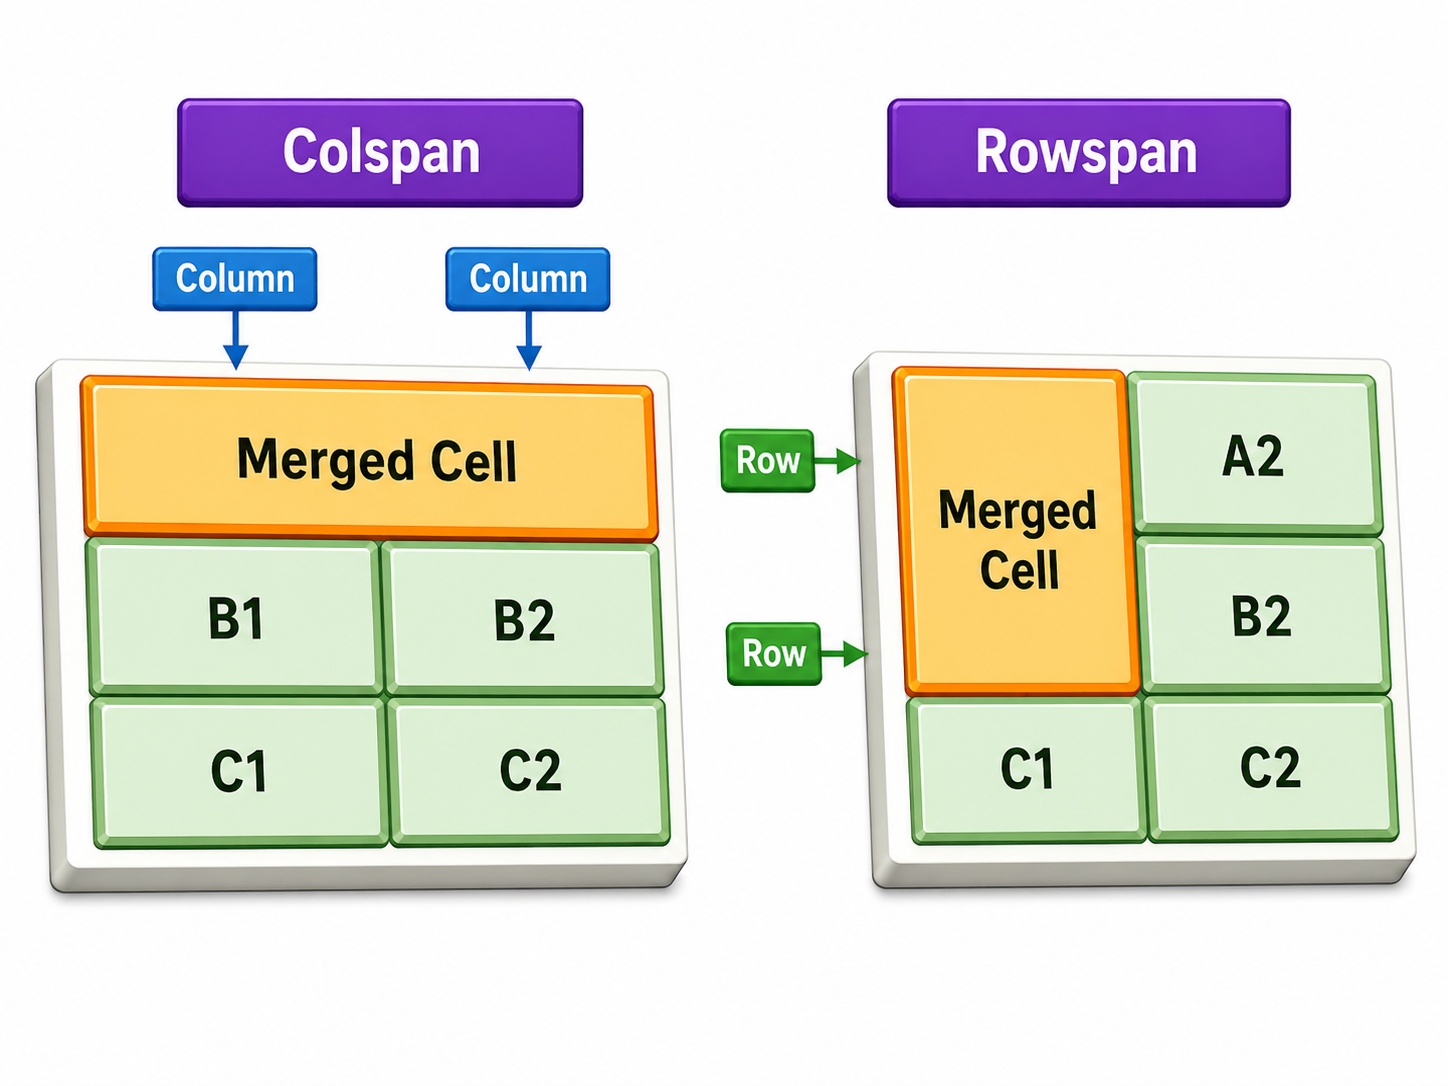
\includegraphics[width=\linewidth,height=.30\textheight,keepaspectratio]{chapters/Chapter04/topics/images/3d_rowspan_colspan.png}
\captionof{figure}{rowspan ও colspan দিয়ে ঘরের বিস্তার}\par\smallskip
\end{minipage}\hfill
\begin{minipage}[t]{.38\linewidth}\vspace{0pt}\small
\begin{keypointbox}{চিত্র ব্যাখ্যা}
চিত্রে \texttt{colspan} দিয়ে আড়াআড়ি বিস্তার এবং \texttt{rowspan} দিয়ে লম্বালম্বি বিস্তার দেখানো হয়েছে। চিত্র দেখে কোড লেখার সময় বিস্তৃত ঘর আগে শনাক্ত করতে হয়।
\end{keypointbox}


\begin{keypointbox}{মনে রাখার উপায়}
\texttt{colspan} = কলাম জুড়ে পাশের দিকে বিস্তার।\\
\texttt{rowspan} = সারি জুড়ে নিচের দিকে বিস্তার।
\end{keypointbox}
\end{minipage}\par\smallskip

\par\noindent\begin{minipage}{\linewidth}
\subsubsection{বিস্তৃত ঘরের দখল করা স্থান গুনে দেখো}
\begin{center}
\begin{tikzpicture}[x=8mm,y=7mm,every node/.style={font=\small,align=center}]
\begin{scope}
\fill[chFourTint] (0,2.6) rectangle (4,3.9);
\draw (0,0) rectangle (6,3.9);
\draw (0,1.3)--(6,1.3) (0,2.6)--(6,2.6);
\draw (2,0)--(2,2.6) (4,0)--(4,3.9);
\node at (2,3.25) {দুই কলাম};
\node at (5,3.25) {এক ঘর};
\node at (3,4.65) {\texttt{colspan="2"}};
\node at (3,-.65) {প্রথম সারিতে দুইটি ট্যাগ};
\end{scope}
\begin{scope}[xshift=65mm]
\fill[chFourRose!10] (0,1.3) rectangle (2,3.9);
\draw (0,0) rectangle (6,3.9);
\draw (0,1.3)--(6,1.3) (2,2.6)--(6,2.6);
\draw (2,0)--(2,3.9) (4,0)--(4,3.9);
\node[text width=14mm] at (1,2.6) {দুই সারি};
\node at (3,4.65) {\texttt{rowspan="2"}};
\node at (3,-.65) {দ্বিতীয় সারিতে দুইটি ট্যাগ};
\end{scope}
\end{tikzpicture}
\captionof{figure}{তিন কলামের ছকে colspan ও rowspan-এর দখল করা স্থান}
\end{center}
বাম ছকে ওপরের একটি ঘর দুই কলামের স্থান নিয়েছে। তাই ওই সারিতে তিন কলামের জন্য দুইটি ঘরের ট্যাগ লিখতে হবে। ডান ছকে বাম ঘরটি প্রথম দুই সারি জুড়ে আছে। দ্বিতীয় সারিতে তার জন্য আরেকটি ট্যাগ লিখলে নতুন ঘর যোগ হয়ে ছক বদলে যাবে। উভয় ছকেই মূল কলামসংখ্যা তিন।

\end{minipage}\par\smallskip

\subsubsection{মূল ছকের স্থান গণনা}

বিস্তৃত ঘর হলো এমন ঘর, যা একাধিক সারি বা কলামের জায়গা নেয়। টেবিল চিত্র দেখে কোড লেখার সময় বিস্তৃত ঘর ভুল হলে পুরো টেবিলের বিন্যাস নষ্ট হয়ে যায়। তাই \texttt{rowspan} ও \texttt{colspan} ব্যবহার করার আগে মূল কলামসংখ্যা ঠিক করা দরকার।

\begin{boardbox}{\texttt{colspan} কখন ব্যবহার করবে}
যদি কোনো ঘর বাম থেকে ডানে একাধিক কলামের জায়গা নেয়, তখন \texttt{colspan} ব্যবহার করবে। যেমন, একটি শিরোনাম যদি টেবিলের তিনটি কলাম জুড়ে থাকে, তাহলে কোড হবে \texttt{<th colspan="3">Title</th>}।
\end{boardbox}

\begin{boardbox}{\texttt{rowspan} কখন ব্যবহার করবে}
যদি কোনো ঘর উপর থেকে নিচে একাধিক সারির জায়গা নেয়, তখন \texttt{rowspan} ব্যবহার করবে। যেমন, একটি বিভাগের নাম যদি দুইটি শাখার সারির জন্য একই হয়, তাহলে কোড হবে \texttt{<td rowspan="2">Science</td>}।
\end{boardbox}

\begin{keypointbox}{বিস্তৃত ঘরের কারণে ঘর গণনা কমে যায়}
\texttt{colspan} দেওয়া ঘর একই সারিতে একাধিক কলামের স্থান নেয়। \texttt{rowspan} দেওয়া ঘর পরের সারির স্থানও দখল করে; সেই পরের সারিতে ওই স্থানের জন্য নতুন ঘর লিখতে হয় না। তাই প্রতিটি সারির দৃশ্যমান ঘর গুনলেই মূল কলামসংখ্যা পাওয়া যায় না; বিস্তৃত ঘরের দখল করা স্থানও ধরতে হবে।
\end{keypointbox}


\subsection{চিত্র থেকে rowspan ও colspan নির্ধারণ}

সারণির চিত্র দেখে কোড লেখার আগে মূল কলাম ও মূল সারিগুলো শনাক্ত করো। বিস্তৃত ঘরটি মূল ছকের কতটি স্থান দখল করেছে, তা গুনতে হয়। শুধু দৃশ্যমান ঘরের সংখ্যা থেকে মূল সারি বা কলামসংখ্যা পাওয়া যায় না। ধাপগুলো হলো:

\begin{enumerate}
\item মোট কয়টি কলাম আছে গুনে নাও।
\item কোনো ঘর ডানদিকে কয়টি কলামজুড়ে আছে দেখো।
\item ঘর ডানদিকে ২টি কলাম জুড়লে \texttt{colspan="2"}।
\item ঘর ডানদিকে ৩টি কলাম জুড়লে \texttt{colspan="3"}।
\item কোনো ঘর নিচের দিকে কয়টি সারিজুড়ে আছে দেখো।
\item ঘর নিচের দিকে ২টি সারি জুড়লে \texttt{rowspan="2"}।
\item ঘর নিচের দিকে ৩টি সারি জুড়লে \texttt{rowspan="3"}।
\item যে সারি বা কলাম একত্র হয়ে গেছে, সেই জায়গার জন্য আলাদা \texttt{<td>} বা \texttt{<th>} আর লিখবে না।
\end{enumerate}

\begin{center}
\begin{tikzpicture}[x=17mm,y=8mm,font=\small]
\draw (0,0) rectangle (3,2);
\draw (0,1)--(3,1);
\draw (1,0)--(1,2);
\draw (2,0)--(2,1);
\node at (.5,1.5) {Name};
\node at (2,1.5) {Subject};
\node at (.5,.5) {1};
\node at (1.5,.5) {2};
\node at (2.5,.5) {3};
\node[anchor=west] at (3.25,1.5) {শিরোনামের ২টি ঘর};
\node[anchor=west] at (3.25,.5) {মূল ছকের ৩টি কলাম};
\end{tikzpicture}
\end{center}
Subject ঘরটি ২ ও ৩ নম্বর কলাম দখল করেছে। তাই প্রথম সারিতে দুটি ঘর লেখা হলেও তার বিস্তার $1+2=3$ কলাম।

\subsection{সবচেয়ে গুরুত্বপূর্ণ নিয়ম}

\subsubsection{colspan হলে একই সারিতে কয়টি ঘর লিখবে?}

নির্দিষ্ট তিন-কলামের সারণিতে একটি ঘর দুই কলামজুড়ে থাকলে বাকি এক কলামের জন্য আরেকটি ঘর প্রয়োজন। তাই শুধু ট্যাগের সংখ্যা নয়, প্রতিটি ঘর কত কলামের স্থান দখল করছে তা যোগ করে দেখবে। নিচের প্রথম সারিটি চাওয়া Name--Math--ICT ছকের সঙ্গে মেলে না: Subject একাই দুই কলামের স্থান নেয়, তার পরে Math ও ICT আরও দুইটি স্থান নেয়।

% Split revision: code and its explanation share one row.
\par\noindent
\begin{minipage}[t]{.50\linewidth}\vspace{0pt}\small
\textbf{ভুল:}
\textbf{\color{chFourTeal}কোড}\par
\begin{verbatim}
<tr>
  <th colspan="2">Subject</th>
  <th>Math</th>
  <th>ICT</th>
</tr>
\end{verbatim}
\par\smallskip
\end{minipage}\hfill
\begin{minipage}[t]{.46\linewidth}\vspace{0pt}\small
\textbf{সঠিক:}
\textbf{\color{chFourTeal}কোড}\par
\begin{verbatim}
<tr>
  <th>Name</th>
  <th colspan="2">Subject</th>
</tr>
<tr>
  <td>Kabir</td>
  <td>Math</td>
  <td>ICT</td>
</tr>
\end{verbatim}
\par\smallskip
\end{minipage}\par


\subsubsection{rowspan হলে পরের সারিতে কী লিখবে?}

যদি একটি ঘর \texttt{rowspan="2"} হয়, তাহলে পরের সারিতে সেই ঘরের জায়গায় আর \texttt{<td>} বা \texttt{<th>} লিখবে না।

\Needspace{7\baselineskip}
% Split revision: code and its explanation share one row.
\par\noindent
\begin{minipage}[t]{.50\linewidth}\vspace{0pt}\small
\textbf{সঠিক:}
\textbf{\color{chFourTeal}কোড}\par
\begin{verbatim}
<tr>
  <th rowspan="2">Phone</th>
  <td>8942318</td>
</tr>
<tr>
  <td>1750181</td>
</tr>
\end{verbatim}
\par\smallskip
\end{minipage}\hfill
\begin{minipage}[t]{.46\linewidth}\vspace{0pt}\small
\textbf{ভুল:}
\textbf{\color{chFourTeal}কোড}\par
\begin{verbatim}
<tr>
  <th rowspan="2">Phone</th>
  <td>8942318</td>
</tr>
<tr>
  <th>Phone</th>
  <td>1750181</td>
</tr>
\end{verbatim}
\par\smallskip
\end{minipage}\par


Phone প্রথম সারি থেকে দ্বিতীয় সারির প্রথম কলাম পর্যন্ত বিস্তৃত আছে। দ্বিতীয় সারিতে আবার Phone-এর ঘর লিখলে সেটি পরের খালি কলামে বসে এবং নম্বর আরও ডানে সরে যায়। ফলে চাওয়া দুই-কলামের ছক পাওয়া যায় না।

\subsection{ফাঁকা ঘর দেখানোর নিয়ম}

খালি \texttt{<td></td>} একটি বৈধ ঘর। সেটি দেখানোর জন্য \texttt{<br>} দেওয়া বাধ্যতামূলক নয়। ঘরের উচ্চতা, ফাঁকা জায়গা ও সীমানা CSS-এর নিয়মের ওপর নির্ভর করে। নিচের পুরোনো উদাহরণে \texttt{<br>} একটি ফাঁকা লাইনের জায়গা রাখে।

\begin{examplebox}{কোড}
\begin{verbatim}
<td><br></td>
\end{verbatim}
\end{examplebox}

নিচের \texttt{\&nbsp;} একটি অচ্ছেদ্য ফাঁকা অক্ষর রাখে; তাই এই ঘরটি আর সম্পূর্ণ খালি থাকে না। এটি ফাঁকা ঘরকে বৈধ করার নিয়ম নয়। নতুন পেজে প্রয়োজনীয় উচ্চতা ও ফাঁকা জায়গা CSS দিয়ে নির্ধারণ করা যায়।

\begin{examplebox}{কোড}
\begin{verbatim}
<td>&nbsp;</td>
\end{verbatim}
\end{examplebox}

\Needspace{7\baselineskip}
\subsection{পূর্ণ অনুশীলন: শিক্ষার্থী ও বিষয়ের সারণি}

% Split revision: code and its explanation share one row.
\par\noindent
\begin{minipage}[t]{.54\linewidth}\vspace{0pt}\small
\textbf{\color{chFourTeal}কোড}\par
\begin{verbatim}
<table border="1" cellspacing="0" cellpadding="5">
  <tr>
    <th colspan="3">Student</th>
  </tr>
  <tr>
    <th>Name</th><th colspan="2">Subject</th>
  </tr>
  <tr>
    <td>Sakib</td><td>Bangla</td><td>English</td>
  </tr>
  <tr>
    <td>Asraful</td><td>Math</td><td>ICT</td>
  </tr>
</table>
\end{verbatim}
\par\smallskip
\end{minipage}\hfill
\begin{minipage}[t]{.42\linewidth}\vspace{0pt}\small
\textbf{\color{chFourTeal}ফলের ধারণা}\par
\begin{center}
\begin{tabular}{|c|c|c|}
\hline
\multicolumn{3}{|c|}{\textbf{Student}} \\
\hline
\textbf{Name} & \multicolumn{2}{c|}{\textbf{Subject}} \\
\hline
Sakib & Bangla & English \\
\hline
Asraful & Math & ICT \\
\hline
\end{tabular}
\end{center}
\par\smallskip
\end{minipage}\par


\Needspace{7\baselineskip}
\subsection{পূর্ণ অনুশীলন: কর্মী ও বেতনের সারণি}

% Split revision: code and its explanation share one row.
\par\noindent
\begin{minipage}[t]{.54\linewidth}\vspace{0pt}\small
\textbf{\color{chFourTeal}কোড}\par
\begin{verbatim}
<table border="1" cellspacing="0" cellpadding="5">
  <caption>Emp. Information</caption>
  <tr>
    <th>ID No</th><th>Emp. Name</th><th>Salary</th>
  </tr>
  <tr>
    <td>1001</td><td>Sakib</td><td rowspan="3">50,000</td>
  </tr>
  <tr>
    <td>1002</td><td>Asraful</td>
  </tr>
  <tr>
    <td><br></td>
    <td><br></td>
  </tr>
</table>
\end{verbatim}
\par\smallskip
\end{minipage}\hfill
\begin{minipage}[t]{.42\linewidth}\vspace{0pt}\small
\textbf{\color{chFourTeal}ফলের ধারণা}\par
\begin{center}
\textbf{Emp. Information}\par\smallskip
\begin{tabular}{|c|c|c|}
\hline
\textbf{ID No} & \textbf{Emp. Name} & \textbf{Salary} \\
\hline
1001 & Sakib & \raisebox{-\normalbaselineskip}[0pt][0pt]{50,000} \\
\cline{1-2}
1002 & Asraful & \\
\cline{1-2}
 & & \\
\hline
\end{tabular}
\end{center}
এখানে Salary-এর 50,000 লেখা ঘরটি তিন সারিজুড়ে আছে; তৃতীয় সারিতে ID No ও Emp. Name ফাঁকা। তাই \texttt{rowspan="3"} দেওয়া হয়েছে। Emp. Information হলো \texttt{<caption>}-এর লেখা; এটি সীমানার ভেতরে একত্র করা শিরোনাম ঘর নয়।
\par\smallskip
\end{minipage}\par



\subsubsection{ভুল ধরো: বাড়তি ঘর কেন হলো?}
\noindent
\begin{minipage}[t]{.48\linewidth}\vspace{0pt}
\textbf{ভুল}\par
\begin{verbatim}
<table border="1">
  <tr><td rowspan="2">ICT</td>
      <td>CQ</td></tr>
  <tr><td>ICT</td><td>MCQ</td></tr>
</table>
\end{verbatim}
\end{minipage}\hfill
\begin{minipage}[t]{.48\linewidth}\vspace{0pt}
\textbf{সঠিক}\par
\begin{verbatim}
<table border="1">
  <tr><td rowspan="2">ICT</td>
      <td>CQ</td></tr>
  <tr><td>MCQ</td></tr>
</table>
\end{verbatim}
\end{minipage}
\chFourWhy{ICT ঘরটি দ্বিতীয় সারির প্রথম স্থানও দখল করেছে। সেখানে নতুন ICT ঘর দিলে মোট তিন কলামের স্থান হয়; দুই-কলামের কাঙ্ক্ষিত ছক পাওয়া যায় না।}
\textbf{পুরোনো ও বর্তমান রীতি:} এখানে \texttt{border} পুরোনো উপস্থাপনমূলক অ্যাট্রিবিউট। আধুনিক CSS-এ ঘরের \texttt{border} ও টেবিলের \texttt{border-collapse} ব্যবহার করবে।



\subsection{প্রয়োগ: নদী ও ফুলের নাম সারণিতে সাজানো}
ফলে River ঘরটি তিনটি সারিজুড়ে থাকবে; পাশে Padma, Jamuna ও Meghna থাকবে। Flower ঘরটিও তিনটি সারিজুড়ে থাকবে; পাশে Adenium, Rose ও Lily থাকবে।

\Needspace{4\baselineskip}
\par\noindent{\color{chFourTeal}\bfseries\small কোড}\par\smallskip
\begin{multicols}{2}
\begin{verbatim}
<!DOCTYPE html>
<html>
<body>
  <table border="1" cellspacing="0" cellpadding="5">
    <tr>
      <td rowspan="3" align="center">River</td><td>Padma</td>
    </tr>
    <tr>
      <td>Jamuna</td>
    </tr>
    <tr>
      <td>Meghna</td>
    </tr>
    <tr>
      <td rowspan="3" align="center">Flower</td><td>Adenium</td>
    </tr>
    <tr>
      <td>Rose</td>
    </tr>
    <tr>
      <td>Lily</td>
    </tr>
  </table>
</body>
</html>
\end{verbatim}
\end{multicols}


\textbf{কেন \texttt{rowspan="3"}?}\\
River-এর পাশে তিনটি নদীর নাম আছে, তাই River ঘর তিনটি সারিজুড়ে থাকবে। Flower-এর ক্ষেত্রেও একই কারণে \texttt{rowspan="3"} ব্যবহার করা হয়েছে।




\subsection{সংক্ষিপ্ত অনুশীলন}

% Each question keeps its answer beneath it in the same column.
\begin{multicols}{2}
\noindent\begin{minipage}[t]{\linewidth}\vspace{0pt}
\chFourReviewQuestion{\textbf{\texttt{colspan} কী?}}
\end{minipage}\par\smallskip
\noindent\begin{minipage}[t]{\linewidth}\vspace{0pt}
\chFourReviewQuestion{\textbf{\texttt{rowspan} কী?}}
\end{minipage}\par\smallskip
\noindent\begin{minipage}[t]{\linewidth}\vspace{0pt}
\chFourReviewQuestion{\textbf{\texttt{rowspan} ও \texttt{colspan}-এর পার্থক্য লেখ।}}
\end{minipage}\par\smallskip
\noindent\begin{minipage}[t]{\linewidth}\vspace{0pt}
\chFourReviewQuestion{\textbf{\texttt{<th colspan="3">Result</th>} এর অর্থ কী?}}
\end{minipage}\par\smallskip
\noindent\begin{minipage}[t]{\linewidth}\vspace{0pt}
\chFourReviewQuestion{\textbf{\texttt{<td rowspan="2">Phone</td>} এর অর্থ কী?}}
\end{minipage}\par\smallskip
\end{multicols}

\Needspace{10\baselineskip}
\subsection{বহুনির্বাচনি অনুশীলন}

\par\addvspace{4pt}\noindent
\begin{minipage}[t]{.48\linewidth}\vspace{0pt}
\begin{enumerate}[start=1,leftmargin=*,topsep=0pt,itemsep=0pt]
\item সারণির ঘরকে একাধিক কলামজুড়ে দিতে কোন অ্যাট্রিবিউট ব্যবহার হয়?
\par ক) \texttt{rowspan}
\par খ) \texttt{colspan}
\par গ) \texttt{cellpadding}
\par ঘ) \texttt{cellspacing}
\end{enumerate}
\end{minipage}\hfill
\begin{minipage}[t]{.48\linewidth}\vspace{0pt}
\begin{enumerate}[start=2,leftmargin=*,topsep=0pt,itemsep=0pt]
\item সারণির ঘরকে একাধিক সারিজুড়ে দিতে কোন অ্যাট্রিবিউট ব্যবহার হয়?
\par ক) \texttt{rowspan}
\par খ) \texttt{colspan}
\par গ) \texttt{border}
\par ঘ) \texttt{src}
\end{enumerate}
\end{minipage}
\par
\par\addvspace{4pt}\noindent
\begin{minipage}[t]{.48\linewidth}\vspace{0pt}
\begin{enumerate}[start=3,leftmargin=*,topsep=0pt,itemsep=0pt]
\item \texttt{<th colspan="4">Title</th>} এর অর্থ কী?
\par ক) Title ৪টি row জুড়ে থাকবে
\par খ) Title ৪টি column জুড়ে থাকবে
\par গ) Title ৪ pixel হবে
\par ঘ) Title ৪ বার দেখা যাবে
\end{enumerate}
\end{minipage}\hfill
\begin{minipage}[t]{.48\linewidth}\vspace{0pt}
\begin{enumerate}[start=4,leftmargin=*,topsep=0pt,itemsep=0pt]
\item \texttt{<td rowspan="3">Phone</td>} এর অর্থ কী?
\par ক) Phone ৩টি column জুড়ে থাকবে
\par খ) Phone ৩টি row জুড়ে থাকবে
\par গ) Phone ৩ pixel হবে
\par ঘ) Phone ৩ বার print হবে
\end{enumerate}
\end{minipage}
\par
\par\addvspace{4pt}\noindent
\begin{minipage}[t]{.48\linewidth}\vspace{0pt}
\begin{enumerate}[start=5,leftmargin=*,topsep=0pt,itemsep=0pt]
\item নিচের কোন ট্যাগে \texttt{rowspan}/\texttt{colspan} ব্যবহার করা যায়?
\par ক) \texttt{<td>} ও \texttt{<th>}
\par খ) \texttt{<br>} ও \texttt{<hr>}
\par গ) \texttt{<img>} ও \texttt{<a>}
\par ঘ) \texttt{<html>} ও \texttt{<body>}
\end{enumerate}
\end{minipage}
\par

\chFourMCQAnswer{১-খ, ২-ক, ৩-খ, ৪-খ, ৫-ক}

\subsection{প্রয়োগ: নম্বরের ছকে দুটি বিস্তৃত শিরোনাম}


\begin{examplebox}{কোড}
\begin{verbatim}
<table border="1" cellspacing="0" cellpadding="5">
  <tr>
    <th colspan="3">Result</th>
  </tr>
  <tr>
    <th>Subject</th><th>CQ</th><th>MCQ</th>
  </tr>
  <tr>
    <td>ICT</td><td>45</td><td>25</td>
  </tr>
  <tr>
    <td>English</td><td colspan="2">95</td>
  </tr>
</table>
\end{verbatim}
\end{examplebox}


\subsection{সৃজনশীল অনুশীলন}

\begin{practicebox}
\textbf{উদ্দীপক:} একটি ওয়েবপেজে Result সারণি দেখাতে হবে। Result শিরোনাম পুরো ৩টি কলামজুড়ে থাকবে এবং English-এর 95 নম্বর CQ ও MCQ--দুইটি কলামজুড়ে থাকবে।

\textbf{প্রশ্ন}\\
ক. \texttt{colspan} কী?\\
খ. \texttt{rowspan} কেন ব্যবহার করা হয়?\\
গ. উদ্দীপকের জন্য HTML কোড লেখ।\\
ঘ. সারণি চিত্র দেখে \texttt{rowspan} ও \texttt{colspan} নির্ধারণের নিয়ম বিশ্লেষণ কর।
\end{practicebox}

\subsection{সাধারণ ভুল}

\begin{mistakebox}{সাধারণ ভুল}
\par\noindent
\begin{minipage}[t]{.48\linewidth}\vspace{0pt}
\begin{itemize}
\item \texttt{rowspan} ও \texttt{colspan} গুলিয়ে ফেলা।
\item কলাম একত্র করতে \texttt{rowspan} ব্যবহার করা।
\item সারি একত্র করতে \texttt{colspan} ব্যবহার করা।
\item \texttt{colspan="2"} দেওয়ার পরও একই সারিতে অতিরিক্ত ঘর লিখে ফেলা।
\item \texttt{rowspan="2"} দেওয়ার পরও পরের সারিতে একই ঘর আবার লিখে ফেলা।
\end{itemize}
\end{minipage}\hfill
\begin{minipage}[t]{.48\linewidth}\vspace{0pt}
\begin{itemize}
\item উদ্ধৃতি না থাকলেই মান ভুল ভাবা: \texttt{colspan=2} বৈধ HTML। তবে একই লেখার রীতি রাখতে \texttt{colspan="2"} ব্যবহার করা সুবিধাজনক।
\item \texttt{<tr>} ট্যাগে \texttt{colspan} লেখা।
\item \texttt{<table>} ট্যাগে \texttt{rowspan} লেখা।
\item চিত্রের মোট সারি/কলাম না গুনে সরাসরি কোড লেখা।
\end{itemize}
\end{minipage}\par

\end{mistakebox}

\begin{boardbox}{পরবর্তী টপিক}
পরের অংশে সারণির ঘরের ভেতরে তালিকা, ছবি, হাইপারলিংক ও নেস্টেড সারণি ব্যবহার করব।
\end{boardbox}

% Density revision 2026-10-04: answers below questions; compact related content.
% Topic 16: Elements ভেতরে HTML সারণি
\section{সারণির ঘরে তালিকা, ছবি, হাইপারলিংক ও নেস্টেড সারণি}

% Composition pass 2026-10-04
লাইব্রেরির তালিকায় একই বইয়ের নাম, প্রচ্ছদ, বিষয় ও বিস্তারিত লিংক একসঙ্গে দরকার।

\chFourMotivation{সম্পর্কিত তথ্য একই ঘরে রাখা $\rightarrow$ ঘরের ভেতর HTML এলিমেন্ট $\rightarrow$ td/th-এর মধ্যে তালিকা, ছবি ও লিংক বসানো $\rightarrow$ বই বা পণ্যের সমন্বিত সারণি।}


\begin{learningbox}
এই অংশ শেষে শিক্ষার্থী পারবে:
\begin{itemize}
\item HTML সারণির ঘরের ভেতরে তালিকা, ছবি, হাইপারলিংক ও ফরম্যাটিং ট্যাগ ব্যবহার করতে।
\item সারণির ঘরের ভেতরে ক্রমিক তালিকা ও অক্রমিক তালিকা বসাতে।
\item ছবির হাইপারলিংক তৈরি করতে।
\item নেস্টেড সারণি কী তা ব্যাখ্যা করতে এবং নেস্টেড সারণির সহজ কোড লিখতে।
\item সৃজনশীল ও ব্যবহারিক প্রশ্নে সারণির ভেতরে একাধিক HTML উপাদান ব্যবহার করে কোড লিখতে।
\end{itemize}
\end{learningbox}



একটি বইয়ের তালিকায় এক কলামে বইয়ের নাম এবং পাশের কলামে তার ছবি, বিষয়গুলোর তালিকা ও বিস্তারিত জানার লিংক দেখাতে চাই। HTML সারণির ঘরে কেবল লেখা নয়; তালিকা, ছবি, হাইপারলিংক ও আরেকটি সারণিও রাখা যায়। এবার আগের ট্যাগগুলো একসঙ্গে ব্যবহার করে এমন চিত্রের কোড লিখব। ঘর ও তার ভেতরের উপাদানের শুরু--শেষ সঠিকভাবে মিলিয়ে রাখাই এখানে প্রধান কাজ।

\subsection{সারণির ঘরে রাখা যায় যেসব উপাদান}

HTML সারণির \texttt{<td>} বা \texttt{<th>} ঘরের ভেতরে অনেক ধরনের HTML উপাদান রাখা যায়।

\begin{center}
\footnotesize
\begin{tabular}{|p{0.30\textwidth}|p{0.52\textwidth}|}
\hline
\textbf{ঘরের ভেতরে রাখা যায়} & \textbf{উদাহরণ} \\
\hline
সাধারণ লেখা & \texttt{<td>ICT</td>} \\
\hline
বোল্ড/আন্ডারলাইন লেখা & \texttt{<td><u>ICT</u></td>} \\
\hline
হাইপারলিংক & \texttt{<td><a href="board.html">Board</a></td>} \\
\hline
ছবি & \texttt{<td><img src="book.jpg" alt="Book" width="100"></td>} \\
\hline
ক্রমিক তালিকা & \texttt{<td><ol><li>Book</li></ol></td>} \\
\hline
অক্রমিক তালিকা & \texttt{<td><ul><li>Pen</li></ul></td>} \\
\hline
নেস্টেড সারণি & \texttt{<td><table>...</table></td>} \\
\hline
\end{tabular}
\end{center}

\begin{keypointbox}{মূল ধারণা}
সারণির ঘরের ভেতরে বিষয়বস্তু রাখার সময় বিষয়বস্তু অবশ্যই \texttt{<td>} বা \texttt{<th>} ট্যাগের ভেতরে রাখতে হবে। \texttt{<table>} ট্যাগের ভেতরে সরাসরি \texttt{<ol>}, \texttt{<ul>}, \texttt{<img>} বা \texttt{<a>} লেখা ঠিক নয়।
\end{keypointbox}

\subsection{সারণির ঘরে তালিকা}

কোনো সারণির ঘরের ভেতরে ক্রমিক তালিকা বা অক্রমিক তালিকা বসাতে হলে \texttt{<td>} ট্যাগের ভেতরে \texttt{<ol>} বা \texttt{<ul>} লিখতে হয়।

\subsubsection{লেখার সাধারণ রূপ}

\begin{examplebox}{কোড}
\begin{verbatim}
<td>
  <ol>
    <li>Item 1</li>
    <li>Item 2</li>
  </ol>
</td>
\end{verbatim}
\end{examplebox}

\Needspace{10\baselineskip}
অথবা--

\begin{examplebox}{কোড}
\begin{verbatim}
<td>
  <ul>
    <li>Item 1</li>
    <li>Item 2</li>
  </ul>
</td>
\end{verbatim}
\end{examplebox}

\subsection{উদাহরণ: ক্রমিক ও অক্রমিক তালিকা}

\begin{examplebox}{ফলের ধারণা}
\begin{center}
\begin{tabular}{|p{0.36\textwidth}|p{0.36\textwidth}|}
\hline
\multicolumn{2}{|c|}{\textbf{A \& H Company Ltd.}} \\
\hline
\textbf{Order List} & \textbf{Unorder List} \\
\hline
i. Book \newline ii. Paper \newline iii. Note Book & \rule{.6ex}{.6ex} Marker \newline \rule{.6ex}{.6ex} Ink \newline \rule{.6ex}{.6ex} Pencil \\
\hline
\end{tabular}
\end{center}
\end{examplebox}

\Needspace{6\baselineskip}
\par\noindent{\color{chFourTeal}\bfseries\small কোড: বাম কলাম শেষে ডান কলাম পড়বে}\par
\begin{multicols}{2}
\begin{verbatim}
<!DOCTYPE html>
<html>
<head>
  <title>HTML List in Table</title>
</head>
<body>
  <table border="2" cellspacing="0" cellpadding="5">
    <tr>
      <th colspan="2" align="center">A & H Company Ltd.</th>
    </tr>
    <tr>
      <th>Order List</th><th>Unorder List</th>
    </tr>
    <tr>
      <td>
        <ol type="i">
          <li>Book</li>
          <li>Paper</li>
          <li>Note Book</li>
        </ol>
      </td>
      <td>
        <ul type="square">
          <li>Marker</li>
          <li>Ink</li>
          <li>Pencil</li>
        </ul>
      </td>
    </tr>
  </table>
</body>
</html>
\end{verbatim}
\end{multicols}


\begin{boardbox}{পরীক্ষার জন্য মনে রাখবে}
ওপরের উদাহরণের Order List ও Unorder List দুটি দৃশ্যমান শিরোনাম। তালিকার সঠিক পরিভাষা Ordered List ও Unordered List। দুই ধরনের তালিকাই ঘরের ভেতরে শুরু ও শেষ হয়েছে।
\end{boardbox}

\subsection{সারণির ঘরে হাইপারলিংক}

সারণির ঘরের ভেতরে লিংক বসাতে \texttt{<td>} ট্যাগের ভেতরে \texttt{<a href="">...</a>} লিখতে হয়।

% Split revision: code and its explanation share one row.
\par\noindent
\begin{minipage}[t]{.54\linewidth}\vspace{0pt}\small
\subsubsection{লেখার রূপ}

\textbf{\color{chFourTeal}কোড}\par
\begin{verbatim}
<td>
  <a href="url">Link Text</a>
</td>
\end{verbatim}
\par\smallskip
\end{minipage}\hfill
\begin{minipage}[t]{.42\linewidth}\vspace{0pt}\small
\subsubsection{উদাহরণ}

\textbf{\color{chFourTeal}কোড}\par
\begin{verbatim}
<td>
  <a href="https://www.educationboard.gov.bd">Board</a>
</td>
\end{verbatim}
\par\smallskip


\texttt{target="\_blank"} দিলে নতুন ব্রাউজিং প্রসঙ্গে লিংক খোলার অনুরোধ করা হয়। ব্রাউজার ও ব্যবহারকারীর সেটিং অনুযায়ী এটি নতুন ট্যাব বা উইন্ডো হতে পারে। বাহ্যিক লিংকে এটি দেওয়া বাধ্যতামূলক নয়; অ্যাট্রিবিউট না দিলে সাধারণত বর্তমান ট্যাবেই পেজ খোলে।
\end{minipage}\par
\subsection{উদাহরণ: বিষয়ের পাশে লিংক}

\begin{examplebox}{ফলের ধারণা}
\begin{center}
\begin{tabular}{|c|c|}
\hline
\textbf{Subject} & \textbf{Board} \\
\hline
ICT & \underline{Board} \\
\hline
\end{tabular}
\end{center}
Board লেখাটি লিংক; এতে ক্লিক করলে \texttt{href}-এ দেওয়া ঠিকানায় যাওয়া যায়।
\end{examplebox}

\begin{examplebox}{কোড}
\begin{verbatim}
<table border="1" cellspacing="0" cellpadding="5">
  <tr>
    <th>Subject</th>
    <th>Board</th>
  </tr>
  <tr>
    <td>ICT</td>
    <td>
      <a href="https://www.educationboard.gov.bd" target="_blank">
        Board
      </a>
    </td>
  </tr>
</table>
\end{verbatim}
\end{examplebox}

\subsection{সারণির ঘরে ছবি}

সারণির ঘরের ভেতরে ছবি বসাতে \texttt{<td>} ট্যাগের ভেতরে \texttt{<img>} ট্যাগ লিখতে হয়।

\subsubsection{লেখার রূপ}

% Split revision: code and its explanation share one row.
\par\noindent
\begin{minipage}[t]{.54\linewidth}\vspace{0pt}\small
\textbf{\color{chFourTeal}কোড}\par
\begin{verbatim}
<td>
  <img src="image.jpg" alt="Image" width="100" height="80">
</td>
\end{verbatim}
\par\smallskip
\end{minipage}\hfill
\begin{minipage}[t]{.42\linewidth}\vspace{0pt}\small
\textbf{\color{chFourTeal}ব্যাখ্যা}\par
এই উদাহরণে \texttt{src} ছবির ঠিকানা এবং \texttt{alt} বিকল্প লেখা জানায়। \texttt{width} ও \texttt{height} ছবির প্রদর্শিত প্রস্থ ও উচ্চতা নির্ধারণ করে।
\end{minipage}\par
\subsection{উদাহরণ: বইয়ের ছবি}

\begin{examplebox}{ফলের ধারণা}
\begin{center}
\begin{tabular}{|c|c|}
\hline
\textbf{Book} & \textbf{Image} \\
\hline
ICT Book & \fbox{\parbox[c][15mm][c]{24mm}{\centering ছবির স্থান\\\texttt{book.jpg}}} \\
\hline
\end{tabular}
\end{center}
\end{examplebox}

\begin{examplebox}{কোড}
\begin{verbatim}
<table border="1" cellspacing="0" cellpadding="5">
  <tr>
    <th>Book</th>
    <th>Image</th>
  </tr>
  <tr>
    <td>ICT Book</td>
    <td>
      <img src="book.jpg" alt="ICT Book" width="100" height="80">
    </td>
  </tr>
</table>
\end{verbatim}
\end{examplebox}

এখানে ছবির জায়গাটি বোঝানো হয়েছে। একই ফোল্ডারে \texttt{book.jpg} থাকলে ব্রাউজারে সেই ছবি দেখা যাবে; ফাইলের নাম দেখানোর নির্দেশ এটি নয়।

\subsection{সারণির ঘরে ছবির হাইপারলিংক}

সারণির ঘরের ছবিতে ক্লিক করে কোনো পেজ বা ওয়েবসাইটে যেতে চাইলে \texttt{<a>} ট্যাগের ভেতরে \texttt{<img>} ট্যাগ বসাতে হবে।

\subsubsection{লেখার রূপ}

\begin{examplebox}{কোড}
\begin{verbatim}
<td>
  <a href="url">
    <img src="image.jpg" alt="Image">
  </a>
</td>
\end{verbatim}
\end{examplebox}

\subsection{উদাহরণ: বইয়ের ছবিতে ক্লিক করে গন্তব্যে যাওয়া}

\begin{examplebox}{কোড}
\begin{verbatim}
<table border="1" cellspacing="0" cellpadding="5">
  <tr>
    <th>Book</th>
    <th>Image Link</th>
  </tr>
  <tr>
    <td>ICT Book</td>
    <td>
      <a href="https://www.book.com" target="_blank">
        <img src="book.jpg" alt="ICT Book" width="100" height="80">
      </a>
    </td>
  </tr>
</table>
\end{verbatim}
\end{examplebox}

\begin{keypointbox}{মনে রাখবে}
ক্লিক করা যায় এমন লেখা তৈরি করতে \texttt{<a>} ট্যাগের ভেতরে লেখা লিখতে হয়। ক্লিক করা যায় এমন ছবি তৈরি করতে \texttt{<a>} ট্যাগের ভেতরে \texttt{<img>} ট্যাগ লিখতে হয়।
\end{keypointbox}

\subsection{তালিকার ভেতরে লিংক: ঘরেও প্রয়োগ করা যায়}

তালিকার উপাদানের ভেতরেও লিংক বসানো যায়। নিচের স্বতন্ত্র তালিকায় Fruits একটি লিংক এবং তার অধীনে Ripe ও Dried উপতালিকা আছে। এখানে \texttt{start="4"} দেওয়ায় উপতালিকার রোমান ক্রম iv ও v থেকে শুরু হয়। এই উদাহরণে সারণি নেই; সারণির ঘরে চাইলে পুরো \texttt{<ul>...</ul>} অংশটি \texttt{<td>...</td>}-এর ভেতরে বসাবে।

\begin{examplebox}{কোড}
\begin{verbatim}
<ul type="circle">
  <li>Vegetables</li>
  <li>
    <a href="https://www.fruitbox.com" target="_blank">Fruits</a>
    <ol type="i" start="4">
      <li>Ripe</li>
      <li>Dried</li>
    </ol>
  </li>
</ul>
\end{verbatim}
\end{examplebox}

\subsection{নেস্টেড সারণির প্রয়োগ}

একটি সারণির ঘরের ভেতরে থাকা আরেকটি সারণিকে নেস্টেড সারণি (Nested Table) বলে। নিচে একজন শিক্ষার্থীর Marks ঘরে বিষয় ও নম্বরের একটি উপসারণি রাখা হয়েছে।

নেস্টেড সারণিতে বাইরের ঘর বন্ধ করার আগে ভেতরের পুরো সারণি বন্ধ করতে হয়। অপ্রয়োজনে বহু স্তরের সারণি করলে কোড পড়া কঠিন হয়। ছোট পর্দায় বিন্যাস ও সহায়ক প্রযুক্তিতে তথ্য বোঝার সমস্যাও হতে পারে। তথ্যের উপসারণি প্রয়োজন হলেই নেস্টেড সারণি ব্যবহার করা উচিত।

\subsection{নেস্টেড সারণি লেখার রূপ}

\begin{examplebox}{কোড}
\begin{verbatim}
<table border="1">
  <tr>
    <td>
      Outer Table Cell
    </td>
    <td>
      <table border="1">
        <tr>
          <td>Inner Table Cell</td>
        </tr>
      </table>
    </td>
  </tr>
</table>
\end{verbatim}
\end{examplebox}

\subsection{উদাহরণ: শিক্ষার্থীর ঘরে নম্বরের সারণি}

\begin{examplebox}{ফলের ধারণা}
\begin{center}
\begin{tabular}{|c|c|}
\hline
\textbf{Student} & \textbf{Marks} \\
\hline
Rafi & \begin{tabular}{|c|c|}\hline
\textbf{Subject} & \textbf{Mark}\\\hline
Bangla & 85\\\hline
English & 90\\\hline
\end{tabular} \\
\hline
\end{tabular}
\end{center}
\end{examplebox}

\Needspace{6\baselineskip}
\par\noindent{\color{chFourTeal}\bfseries\small কোড: বাম কলাম শেষে ডান কলাম পড়বে}\par
\begin{multicols}{2}
\begin{verbatim}
<table border="1" cellspacing="0" cellpadding="5">
  <tr>
    <th>Student</th><th>Marks</th>
  </tr>
  <tr>
    <td>Rafi</td>
    <td>
      <table border="1" cellspacing="0" cellpadding="5">
        <tr>
          <th>Subject</th><th>Mark</th>
        </tr>
        <tr>
          <td>Bangla</td><td>85</td>
        </tr>
        <tr>
          <td>English</td><td>90</td>
        </tr>
      </table>
    </td>
  </tr>
</table>
\end{verbatim}
\end{multicols}


\Needspace{11\baselineskip}
\subsection{নেস্টেড সারণিতে যে নিয়মগুলো দেখবে}

\begin{mistakebox}{সতর্কতা}
\begin{itemize}
\item অনেক স্তরের নেস্টেড সারণির কোড পড়া কঠিন হয়।
\item ভুল সমাপ্তি ট্যাগ দিলে বিন্যাস নষ্ট হয়।
\item সহায়ক প্রযুক্তিতে ব্যবহারের সমস্যা হতে পারে।
\item ছোট পর্দায় বিন্যাসে সমস্যা হতে পারে।
\item শুধুমাত্র সারণিভিত্তিক তথ্যের ভেতরে উপসারণি দরকার হলে ব্যবহার করা উচিত।
\end{itemize}
\end{mistakebox}

\begin{boardbox}{ব্যবহারের ক্ষেত্র}
নেস্টেড সারণি দিয়ে সারণির ভেতরে তথ্যের উপসারণি দেখানো যায়। পুরো ওয়েবপেজের বিন্যাস তৈরির জন্য আধুনিক ওয়েব ডিজাইনে CSS ব্যবহার করবে।
\end{boardbox}

\subsection{একটি ঘরে একাধিক উপাদান}

একটি ঘরের ভেতরে একাধিক উপাদান একসঙ্গে থাকতে পারে।

% Split revision: code and its explanation share one row.
\par\noindent
\begin{minipage}[t]{.54\linewidth}\vspace{0pt}\small
\textbf{\color{chFourTeal}কোড}\par
\begin{verbatim}
<td>
  <h3>ICT Book</h3>
  <img src="book.jpg" alt="ICT Book" width="100">
  <p>Price: 300 Tk</p>
  <a href="book.html">Details</a>
</td>
\end{verbatim}
\par\smallskip
\end{minipage}\hfill
\begin{minipage}[t]{.42\linewidth}\vspace{0pt}\small
\textbf{\color{chFourTeal}ব্যাখ্যা}\par
এখানে একই ঘরের ভেতরে শিরোনাম, ছবি, অনুচ্ছেদ ও লিংক আছে।
\end{minipage}\par
\subsection{পূর্ণ অনুশীলন: সারণি, তালিকা, ছবি ও লিংক}

\begin{examplebox}{ফলের ধারণা}
\begin{center}
\textbf{ICT Learning Materials}\par\smallskip
\begin{tabular}{|c|l|}
\hline
\textbf{Item} & \textbf{Details} \\
\hline
Book & \begin{tabular}{@{}c@{}}\fbox{\parbox[c][15mm][c]{24mm}{\centering ছবির স্থান\\\texttt{book.jpg}}}\\\underline{Buy Book}\end{tabular} \\
\hline
Subjects & \begin{tabular}{@{}l@{}}1. Web Design\\2. HTML\\3. Database\end{tabular} \\
\hline
\end{tabular}
\end{center}
\end{examplebox}

\Needspace{6\baselineskip}
\par\noindent{\color{chFourTeal}\bfseries\small কোড: বাম কলাম শেষে ডান কলাম পড়বে}\par
\begin{multicols}{2}
\begin{verbatim}
<table border="1" cellspacing="0" cellpadding="5">
  <caption>ICT Learning Materials</caption>
  <tr>
    <th>Item</th><th>Details</th>
  </tr>
  <tr>
    <td>Book</td>
    <td>
      <a href="https://www.book.com" target="_blank">
        <img src="book.jpg" alt="ICT Book" width="100" height="80">
      </a>
      <br>
      <a href="https://www.book.com" target="_blank">Buy Book</a>
    </td>
  </tr>
  <tr>
    <td>Subjects</td>
    <td>
      <ol type="1">
        <li>Web Design</li>
        <li>HTML</li>
        <li>Database</li>
      </ol>
    </td>
  </tr>
</table>
\end{verbatim}
\end{multicols}


ওপরের পূর্ণ অনুশীলনে ছবির জায়গা ও Buy Book লিংক দেখানো হয়েছে। ছবিতে বা লেখায় ক্লিক করলে কোডের গন্তব্যে যাওয়া যায়। পরের সৃজনশীল অনুশীলনটি স্বতন্ত্র; সেখানে Subjects-এর তালিকা HTML, CSS ও JavaScript। বাহ্যিক ঠিকানাগুলো লিংকের গঠন শেখানোর উদাহরণ; প্রয়োজনমতো বৈধ গন্তব্য ব্যবহার করবে।

% Original applied explanation; see Chapter04/SOURCES.md.
\subsubsection{ঘরের ভেতরের তথ্য ও বাইরের ঘর এক নয়}
গ্রন্থাগারের বইয়ের সারণিতে একটি ঘরে বইয়ের নাম, আরেক ঘরে প্রচ্ছদের ছবি এবং তৃতীয় ঘরে বিস্তারিত পেজের লিংক রাখা যায়। লেখা, \texttt{img} বা \texttt{a} সংশ্লিষ্ট \texttt{td}-এর ভেতরে থাকবে। সরাসরি \texttt{tr}-এর মধ্যে ছবি বসালে ঘরের গঠন ঠিক থাকে না।

এক ঘরের ভেতরে ছোট সারণি থাকলে আগে বাইরের ঘর খুলবে, তার ভেতরে সম্পূর্ণ ভেতরের সারণি লিখবে, তারপর বাইরের ঘর বন্ধ করবে। বাইরের ও ভেতরের \texttt{tr} আলাদা সারণির সারি; তাদের একসঙ্গে গুনবে না।

\subsection{প্রয়োগ: ঘরের লেখা, লিংক, ছবি ও তালিকা}

টেবিলের ঘরের ভিতরে লেখা ছাড়াও অন্য HTML এলিমেন্ট রাখা যায়। এখানে ছবি, তালিকা, ফর্মের নিয়ন্ত্রণ, আড়াআড়ি রেখা, হাইপারলিংক এবং আরেকটি টেবিল রাখার উদাহরণ আছে। ফলে ফলাফলের সঙ্গে শিক্ষার্থীর ছবি, পণ্যের তালিকার সঙ্গে কেনার লিংক এবং কোর্স পরিকল্পনার সঙ্গে ক্রমযুক্ত তালিকা দেখানো যায়। বিস্তারিত তথ্যের জন্য কোনো ঘরে আরেকটি টেবিলও রাখা যায়।

\begin{keypointbox}{ঘরের ভিতরে বিষয়বস্তু রাখার নিয়ম}
ঘরের ভিতরে বিষয়বস্তু রাখতে হলে বিষয়বস্তু অবশ্যই \texttt{<td>} বা \texttt{<th>} ট্যাগের শুরুর ও শেষের ট্যাগের মাঝখানে লিখতে হবে। যেমন ছবি বসাতে \texttt{<td><img src="photo.jpg"></td>} এবং লিংক বসাতে \texttt{<td><a href="page.html">Open</a></td>} লিখতে হবে।
\end{keypointbox}

\begin{center}
\begin{tabular}{|p{0.22\textwidth}|p{0.50\textwidth}|p{0.18\textwidth}|}
\hline
\textbf{বিষয়বস্তুর ধরন} & \textbf{ঘরের ভিতরে কোডের উদাহরণ} & \textbf{ট্যাগ} \\
\hline
লেখা & \texttt{<td>Rafi</td>} & \texttt{<td>} \\
\hline
ছবি & \texttt{<td><img src="a.jpg"></td>} & \texttt{<img>} \\
\hline
লিংক & \texttt{<td><a href="a.html">Open</a></td>} & \texttt{<a>} \\
\hline
তালিকা & \texttt{<td><ol>...</ol></td>} & \texttt{<ol>}, \texttt{<li>} \\
\hline
আড়াআড়ি রেখা & \texttt{<td><hr></td>} & \texttt{<hr>} \\
\hline
ফর্মের নিয়ন্ত্রণ & \texttt{<td><input type="text"></td>} & \texttt{<input>} \\
\hline
ভেতরের টেবিল & \texttt{<td><table>...</table></td>} & \texttt{<table>} \\
\hline
\end{tabular}
\end{center}

% Image layout revision: related content in two fixed columns.
\par\noindent
\begin{minipage}[t]{.48\linewidth}\vspace{0pt}\small
\subsubsection{লেখার বিন্যাস}
\begin{chFourWholeExample}{কোড}
\begin{verbatim}
<table border="1" cellspacing="0" cellpadding="6">
  <tr>
    <td><b>ICT</b></td>
    <td><u>HSC</u></td>
    <td><i>Book</i></td>
  </tr>
</table>
\end{verbatim}
\end{chFourWholeExample}
\end{minipage}\hfill
\begin{minipage}[t]{.48\linewidth}\vspace{0pt}\small
\subsubsection{হাইপারলিংক}
\begin{chFourWholeExample}{কোড}
\begin{verbatim}
<table border="1" cellspacing="0" cellpadding="6">
  <tr>
    <td>
      <a href="https://www.educationboard.gov.bd">Education Board</a>
    </td>
  </tr>
</table>
\end{verbatim}
\end{chFourWholeExample}
\end{minipage}\par\smallskip
% Image layout revision: related content in two fixed columns.
\par\noindent
\begin{minipage}[t]{.48\linewidth}\vspace{0pt}\small
\subsubsection{ছবি}
\begin{chFourWholeExample}{কোড}
\begin{verbatim}
<table border="1" cellspacing="0" cellpadding="6">
  <tr>
    <td>
      <img src="photo.jpg" width="100" height="80" alt="Photo">
    </td>
  </tr>
</table>
\end{verbatim}
\end{chFourWholeExample}
\end{minipage}\hfill
\begin{minipage}[t]{.48\linewidth}\vspace{0pt}\small
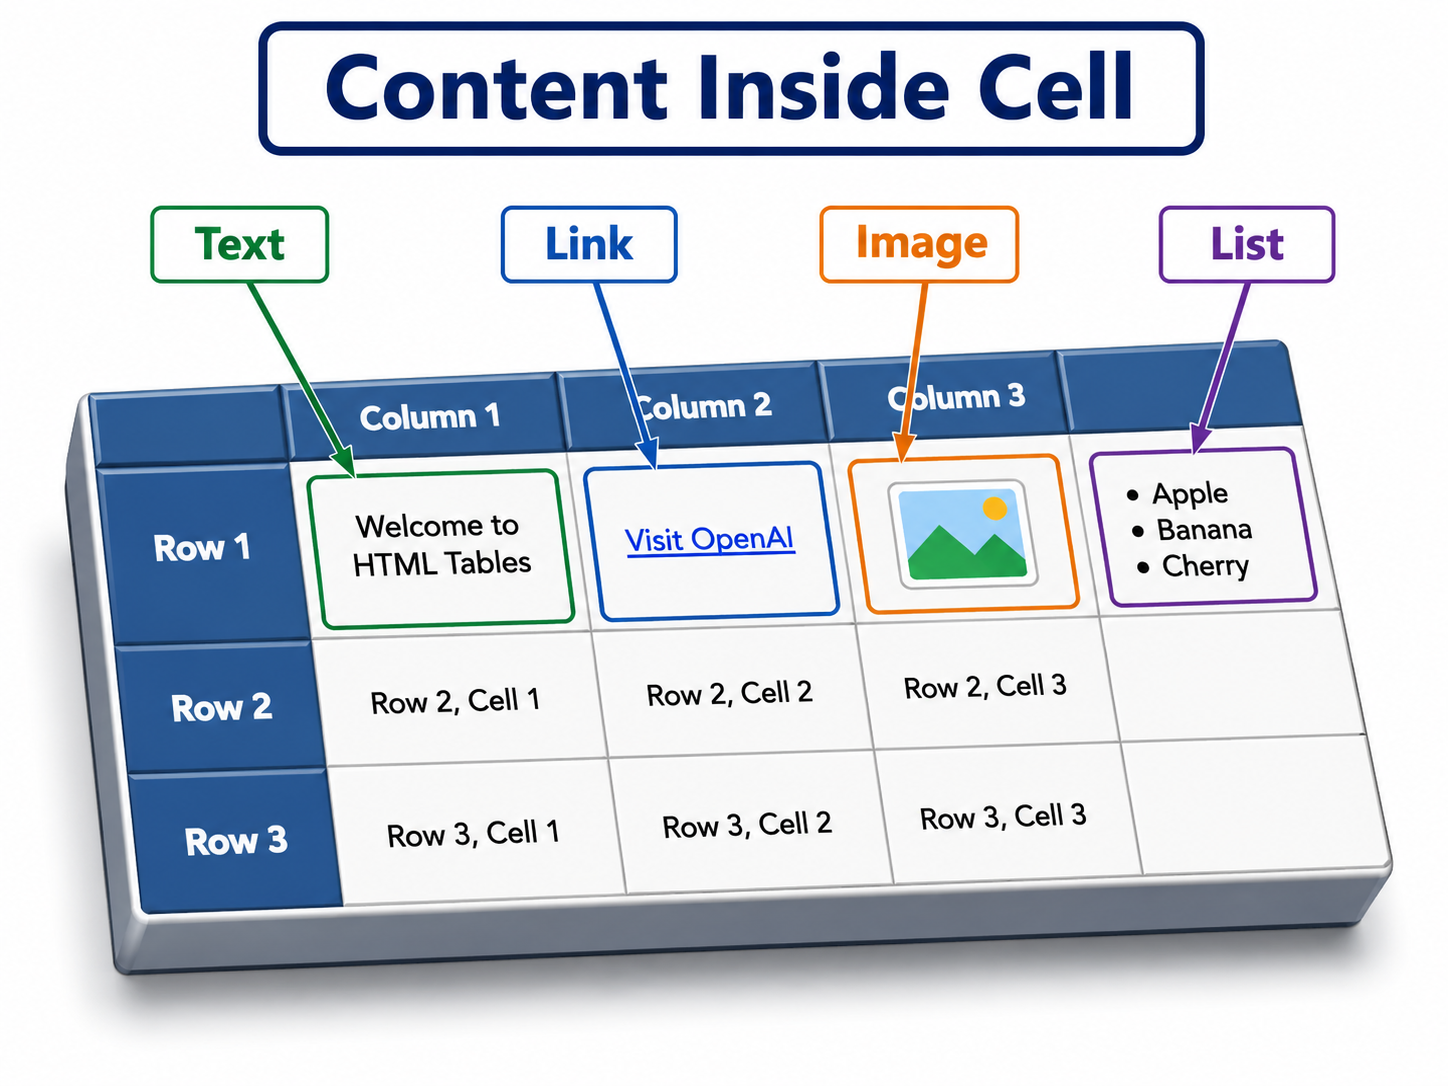
\includegraphics[width=\linewidth,height=.30\textheight,keepaspectratio]{chapters/Chapter04/topics/images/3d_content_inside_cell.png}
\captionof{figure}{টেবিলের ঘরের ভিতরে লেখা, লিংক, ছবি ও তালিকা}\par\smallskip
\end{minipage}\par\smallskip
\subsubsection{তালিকা}
% Image layout revision: related content in two fixed columns.
\par\noindent
\begin{minipage}[t]{.52\linewidth}\vspace{0pt}\small
\begin{chFourWholeExample}{কোড}
\begin{verbatim}
<table border="1" cellspacing="0" cellpadding="6">
  <tr>
    <td>
      <ol>
        <li>Dhaka</li>
        <li>Dinajpur</li>
        <li>Rangpur</li>
      </ol>
    </td>
  </tr>
</table>
\end{verbatim}
\end{chFourWholeExample}
\end{minipage}\hfill
\begin{minipage}[t]{.44\linewidth}\vspace{0pt}\small
\noindent{\color{chFourTeal}\bfseries চিত্র ব্যাখ্যা:}
চিত্রে টেবিলের ঘরের ভিতরে চার ধরনের বিষয়বস্তু দেখানো হয়েছে: সাধারণ লেখা, হাইপারলিংক, ছবি এবং ক্রমযুক্ত তালিকা। তালিকা থাকা ঘরে \texttt{<ol>} ও \texttt{<li>} ট্যাগ ব্যবহার করা হয়েছে।

\begin{keypointbox}{চিত্র দেখে কোড লেখার ধাপ}
যে ঘরের ভিতরে তালিকা থাকবে, সেখানে প্রথমে \texttt{<td>} লিখবে। তারপর ঘরের ভিতরে \texttt{<ol>} বা \texttt{<ul>} ট্যাগ লিখে তালিকার প্রতিটি বিষয় \texttt{<li>} দিয়ে লিখবে।
\end{keypointbox}
\end{minipage}\par\smallskip

\subsection{প্রয়োগ: Parent Cell-এর পাশে উপসারণি}

% Image layout revision: related content in two fixed columns.
\par\noindent
\begin{minipage}[t]{.52\linewidth}\vspace{0pt}\small
\begin{examplebox}{কোড}
\begin{verbatim}
<table border="1" cellspacing="0" cellpadding="10">
  <tr>
    <td>Parent Cell</td>
    <td>
      <table border="1" cellspacing="0" cellpadding="5">
        <tr>
          <th>Child</th><th>Table</th>
        </tr>
        <tr>
          <td>A</td><td>B</td>
        </tr>
      </table>
    </td>
  </tr>
</table>
\end{verbatim}
\end{examplebox}
\end{minipage}\hfill
\begin{minipage}[t]{.44\linewidth}\vspace{0pt}\small
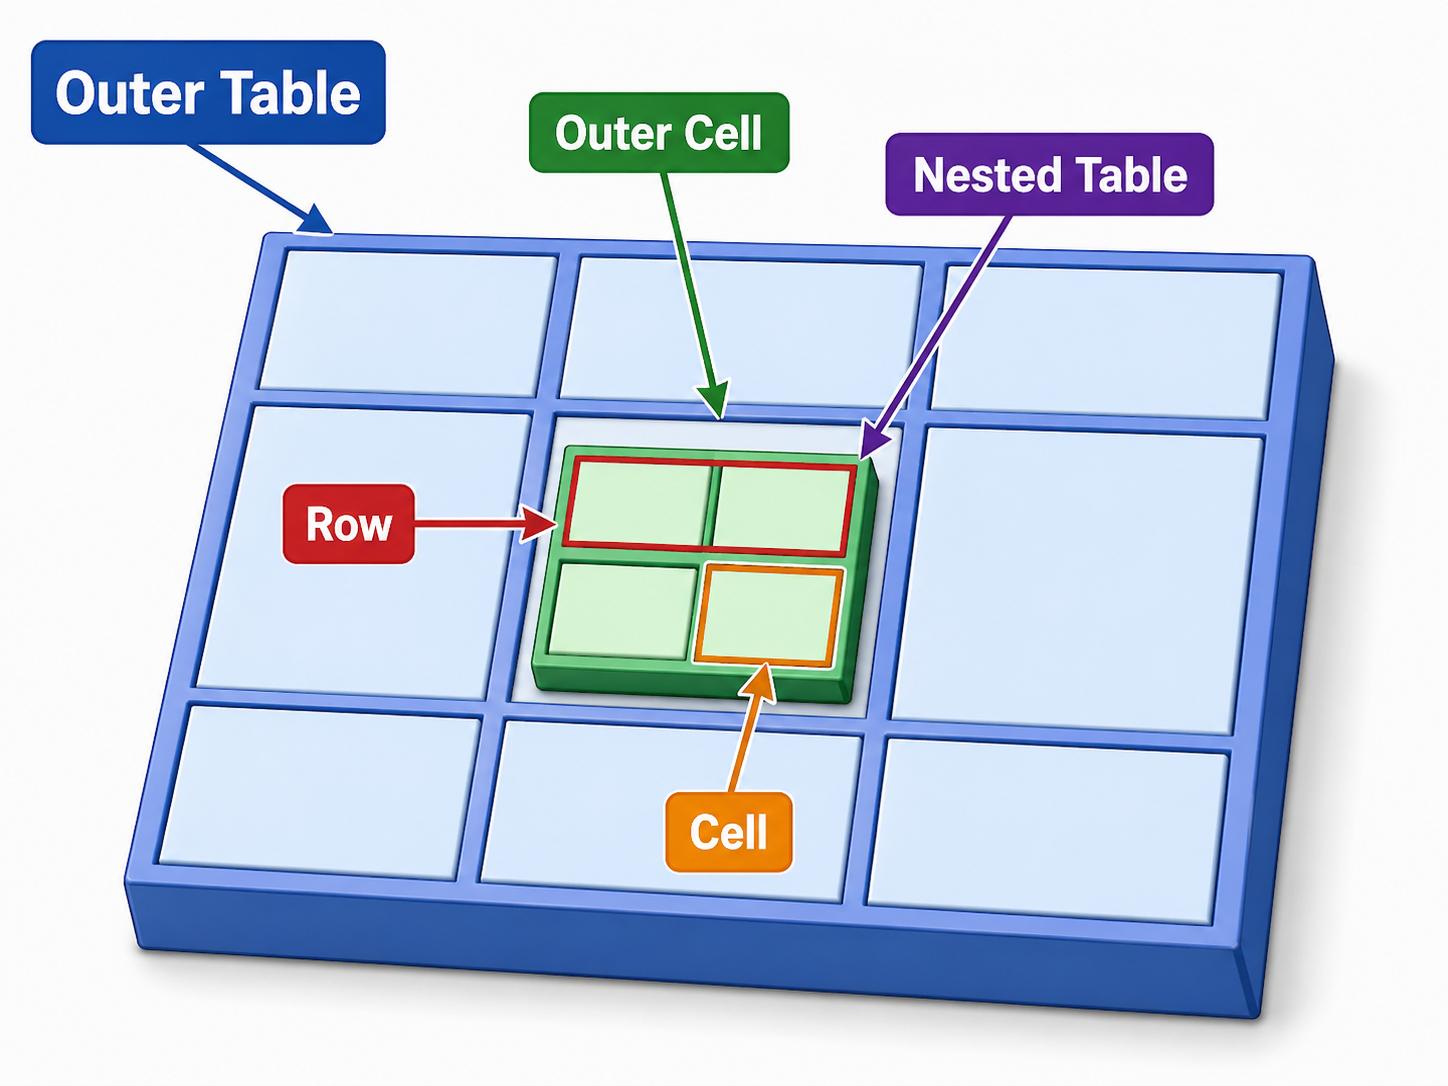
\includegraphics[width=\linewidth,height=.30\textheight,keepaspectratio]{chapters/Chapter04/topics/images/3d_nested_table.png}
\captionof{figure}{টেবিলের ভিতরে ভেতরের টেবিল}\par\smallskip

\textbf{\color{chFourTeal}চিত্র ব্যাখ্যা:} চিত্রে বাইরের টেবিলের একটি ঘরের ভিতরে ভেতরের টেবিল বসানো হয়েছে। এটিকে ভেতরের টেবিল বা টেবিলের ভিতরে টেবিল বলা হয়।
\end{minipage}\par\smallskip


\begin{keypointbox}{ভেতরের টেবিল লেখার সতর্কতা}
ভেতরের টেবিল লিখলে বাইরের টেবিল ও ভেতরের টেবিলের ট্যাগ আলাদা করে শেষ করতে হবে। প্রথমে ভেতরের টেবিলের \texttt{</table>} শেষ করবে, তারপর বাইরের টেবিলের ঘরের \texttt{</td>} এবং শেষে বাইরের টেবিল শেষ করবে। ভুল জায়গায় \texttt{</table>} দিলে প্রদর্শিত টেবিলের বিন্যাস ভেঙে যায়।
\end{keypointbox}



\subsection{সংক্ষিপ্ত অনুশীলন}

% Each question keeps its answer beneath it in the same column.
\begin{multicols}{2}
\noindent\begin{minipage}[t]{\linewidth}\vspace{0pt}
\chFourReviewQuestion{\textbf{সারণির ঘরের ভেতরে তালিকা কীভাবে লেখা যায়?}}
\end{minipage}\par\smallskip
\noindent\begin{minipage}[t]{\linewidth}\vspace{0pt}
\chFourReviewQuestion{\textbf{সারণির ভেতরে হাইপারলিংক কীভাবে তৈরি করা যায়?}}
\end{minipage}\par\smallskip
\noindent\begin{minipage}[t]{\linewidth}\vspace{0pt}
\chFourReviewQuestion{\textbf{সারণির ভেতরে ছবি কীভাবে বসানো যায়?}}
\end{minipage}\par\smallskip
\noindent\begin{minipage}[t]{\linewidth}\vspace{0pt}
\chFourReviewQuestion{\textbf{নেস্টেড সারণি কী?}}
\end{minipage}\par\smallskip
\noindent\begin{minipage}[t]{\linewidth}\vspace{0pt}
\chFourReviewQuestion{\textbf{ছবির হাইপারলিংক কীভাবে তৈরি করা যায়?}}
\end{minipage}\par\smallskip
\end{multicols}

\Needspace{10\baselineskip}
\subsection{বহুনির্বাচনি অনুশীলন}

\begin{multicols}{2}
\begin{enumerate}[leftmargin=*,itemsep=5pt]
\item \begin{minipage}[t]{\linewidth}\vspace{0pt}
সারণির ঘরের ভেতরে ছবি বসাতে কোন ট্যাগ ব্যবহার হয়?
\par ক) \texttt{<a>}
\par খ) \texttt{<img>}
\par গ) \texttt{<ol>}
\par ঘ) \texttt{<tr>}
\end{minipage}

\item \begin{minipage}[t]{\linewidth}\vspace{0pt}
সারণির ঘরের ভেতরে লিংক তৈরি করতে কোন ট্যাগ ব্যবহার হয়?
\par ক) \texttt{<a>}
\par খ) \texttt{<td>}
\par গ) \texttt{<br>}
\par ঘ) \texttt{<hr>}
\end{minipage}

\item \begin{minipage}[t]{\linewidth}\vspace{0pt}
সারণির ঘরের ভেতরে ক্রমিক তালিকা বসাতে কোন ট্যাগ ব্যবহার হবে?
\par ক) \texttt{<ul>}
\par খ) \texttt{<ol>}
\par গ) \texttt{<img>}
\par ঘ) \texttt{<caption>}
\end{minipage}

\item \begin{minipage}[t]{\linewidth}\vspace{0pt}
ছবির হাইপারলিংক তৈরির সঠিক গঠন কোনটি?
\par ক) \texttt{<img href="home.html">}
\par খ) \texttt{<a href="home.html"><img src="logo.png" alt="Logo"></a>}
\par গ) \texttt{<a src="logo.png">Home</a>}
\par ঘ) \texttt{<table img="logo.png">}
\end{minipage}

\item \begin{minipage}[t]{\linewidth}\vspace{0pt}
একটি সারণির ঘরের ভেতরে আরেকটি সারণি থাকলে তাকে কী বলে?
\par ক) Empty Table
\par খ) Nested Table
\par গ) Ordered Table
\par ঘ) External Table
\end{minipage}
\end{enumerate}
\end{multicols}

\chFourMCQAnswer{১-খ, ২-ক, ৩-খ, ৪-খ, ৫-খ}

\subsection{প্রয়োগ: একটি ছকে বইয়ের ছবি, লিংক ও বিষয়}


\Needspace{6\baselineskip}
\par\noindent{\color{chFourTeal}\bfseries\small কোড: বাম কলাম শেষে ডান কলাম পড়বে}\par
\begin{multicols}{2}
\begin{verbatim}
<table border="1" cellspacing="0" cellpadding="5">
  <caption>ICT Learning Materials</caption>
  <tr>
    <th>Item</th><th>Details</th>
  </tr>
  <tr>
    <td>Book</td>
    <td>
      <a href="book.html">
        <img src="book.jpg" alt="ICT Book" width="100" height="80">
      </a>
    </td>
  </tr>
  <tr>
    <td>Subjects</td>
    <td>
      <ol>
        <li>HTML</li>
        <li>CSS</li>
        <li>JavaScript</li>
      </ol>
    </td>
  </tr>
</table>
\end{verbatim}
\end{multicols}



\subsection{সৃজনশীল অনুশীলন}

\begin{practicebox}
\textbf{উদ্দীপক:} একটি ওয়েবপেজে ``ICT Learning Materials'' নামে একটি সারণি তৈরি করতে হবে। সারণিতে দুইটি কলাম থাকবে: Item ও Details। Book সারির Details ঘরে \texttt{book.jpg} ছবি থাকবে এবং ছবিতে ক্লিক করলে \texttt{book.html} পেজ খোলা হবে। Subjects সারির Details ঘরে ক্রমিক তালিকা হিসেবে HTML, CSS, JavaScript থাকবে।

\textbf{প্রশ্ন}\\
ক. নেস্টেড সারণি কী?\\
খ. ছবির হাইপারলিংক তৈরির নিয়ম ব্যাখ্যা কর।\\
গ. উদ্দীপকের জন্য HTML কোড লেখ।\\
ঘ. সারণির ঘরের ভেতরে তালিকা, ছবি ও হাইপারলিংক ব্যবহারের সুবিধা বিশ্লেষণ কর।
\end{practicebox}

\subsection{সাধারণ ভুল}

\begin{mistakebox}{সাধারণ ভুল}
\par\noindent
\begin{minipage}[t]{.48\linewidth}\vspace{0pt}
\begin{itemize}
\item \texttt{<td>} ট্যাগের বাইরে তালিকা লিখে ফেলা।
\item \texttt{<td>} শেষ করার আগে \texttt{<ol>} বা \texttt{<ul>} ঠিকভাবে শেষ না করা।
\item ছবির লিংক করতে \texttt{<a>} ট্যাগের ভেতরে \texttt{<img>} না রাখা।
\item \texttt{href} ও \texttt{src} অ্যাট্রিবিউট গুলিয়ে ফেলা।
\end{itemize}
\end{minipage}\hfill
\begin{minipage}[t]{.48\linewidth}\vspace{0pt}
\begin{itemize}
\item \texttt{<table>} ট্যাগের ভেতরে সরাসরি \texttt{<ol>} লিখে ফেলা; ঘর দরকার।
\item নেস্টেড সারণির সমাপ্তি ট্যাগ ভুল করা।
\item সারণির ঘরের ভেতরে বিষয়বস্তু বেশি দিলে বিন্যাস অগোছালো করা।
\item সব বাহ্যিক লিংকে \texttt{target="\_blank"} বাধ্যতামূলক ভাবা; এটি নতুন ট্যাব/উইন্ডোতে খোলার প্রয়োজন অনুযায়ী দেওয়া হয়।
\end{itemize}
\end{minipage}\par

\end{mistakebox}

\begin{boardbox}{পরবর্তী টপিক}
পরের অংশে \texttt{<div>}, \texttt{<span>} ও \texttt{style} অ্যাট্রিবিউট দিয়ে বিষয়বস্তু সাজানো এবং ইনলাইন CSS-এর মৌলিক প্রয়োগ দেখব।
\end{boardbox}

\setcounter{collectmore}{-4}

% Density revision 2026-10-04: answers below questions; compact related content.
% Topic 17: Division, Span and style অ্যাট্রিবিউট
\section{বিভাগ, ইনলাইন অংশ ও রীতি: div, span ও style}

% Composition pass 2026-10-04
পুরো বিজ্ঞপ্তির পটভূমি বদলাতে হবে, আবার একটি বাক্যের শুধু শেষ তারিখ আলাদা রঙে দেখাতে হবে।

\chFourMotivation{বড় অংশ ও ছোট লেখাংশ আলাদা করা $\rightarrow$ div ও span $\rightarrow$ নির্বাচিত ধারকে CSS প্রয়োগ $\rightarrow$ কলেজের বিজ্ঞপ্তি সুস্পষ্ট হয়।}


\begin{learningbox}
এই অংশ শেষে শিক্ষার্থী পারবে:
\begin{itemize}
\item \texttt{<div>} ট্যাগের কাজ ও ব্যবহার ব্যাখ্যা করতে।
\item \texttt{<span>} ট্যাগের কাজ ও ব্যবহার ব্যাখ্যা করতে।
\item \texttt{<div>} ও \texttt{<span>}-এর পার্থক্য লিখতে।
\item \texttt{style} অ্যাট্রিবিউট ব্যবহার করে ইনলাইন CSS লিখতে।
\item \texttt{color}, \texttt{background-color}, \texttt{font-size}, \texttt{text-align}, \texttt{margin}, \texttt{padding}, \texttt{border} ইত্যাদি মৌলিক CSS প্রোপার্টি ব্যবহার করতে।
\end{itemize}
\end{learningbox}



আগের পাঠগুলোতে আমরা HTML দিয়ে শিরোনাম, অনুচ্ছেদ, তালিকা, হাইপারলিংক, ছবি ও সারণি তৈরি করেছি। এখন ওয়েবপেজের বিভিন্ন অংশ একসঙ্গে রাখা এবং নির্দিষ্ট অংশে রীতি প্রয়োগ করা শিখব। এই পাঠে তিনটি বিষয় সবচেয়ে গুরুত্বপূর্ণ: \texttt{<div>}, \texttt{<span>} এবং \texttt{style} অ্যাট্রিবিউট।

\subsection{\texttt{<div>} ট্যাগ কী?}

\begin{definitionbox}{বিভাগের ধারক (div Element)}
একাধিক HTML এলিমেন্টকে একটি সাধারণ ধারকে দলবদ্ধ করতে \texttt{<div>} ট্যাগ ব্যবহার করা হয়।
\end{definitionbox}

\texttt{<div>}-এ পেজের একটি বড় অংশের শিরোনাম, অনুচ্ছেদ ও অন্যান্য এলিমেন্ট রাখা যায়। ধারকটি নিজে বিশেষ নকশা তৈরি করে না। CSS প্রয়োগ করে পুরো অংশের পটভূমি, সীমানা ও অবস্থান একসঙ্গে নির্ধারণ করা যায়।

% Split revision: code and its explanation share one row.
\par\noindent
\begin{minipage}[t]{.42\linewidth}\vspace{0pt}\small
\subsubsection{সিনট্যাক্স}

\textbf{\color{chFourTeal}কোড}\par
\begin{verbatim}
<div>
  Content here
</div>
\end{verbatim}

\par\smallskip
\end{minipage}\hfill
\begin{minipage}[t]{.54\linewidth}\vspace{0pt}\small
\subsubsection{উদাহরণ}

\textbf{\color{chFourTeal}কোড}\par
\begin{verbatim}
<div>
  <h2>About College</h2>
  <p>ABC College is a reputed institution.</p>
</div>
\end{verbatim}

\par\smallskip


এখানে শিরোনাম ও অনুচ্ছেদ একই ধারকে রাখা হয়েছে।
\end{minipage}\par
\subsection{\texttt{<div>} ট্যাগের ব্যবহার}

\texttt{<div>} সাধারণত ওয়েবপেজের বড় অংশ ভাগ করতে ব্যবহৃত হয়।

\par\noindent
\begin{minipage}[t]{.48\linewidth}\vspace{0pt}
\begin{itemize}
\item হেডার অংশ তৈরি করতে
\item চলাচল/মেনু এলাকা একসঙ্গে রাখতে
\item প্রধান বিষয়বস্তু অংশ তৈরি করতে
\item পাশের অংশ তৈরি করতে
\end{itemize}
\end{minipage}\hfill
\begin{minipage}[t]{.48\linewidth}\vspace{0pt}
\begin{itemize}
\item ফুটার অংশ তৈরি করতে
\item একাধিক এলিমেন্ট একসঙ্গে রীতি প্রয়োগ করতে
\item ওয়েবপেজ বিন্যাস তৈরি করতে
\end{itemize}
\end{minipage}\par


\Needspace{7\baselineskip}
\subsection{উদাহরণ: পেজের অংশ}

% Split revision: code and its explanation share one row.
\par\noindent
\begin{minipage}[t]{.60\linewidth}\vspace{0pt}\small
\textbf{\color{chFourTeal}কোড}\par
\par\noindent
\begin{verbatim}
<!DOCTYPE html><html>
<head><title>Div Example</title></head>
<body>
  <div style="background-color:lightblue; padding:10px;">
    <h1>ABC College</h1>
    <p>Welcome to our official website.</p>
  </div>
  <div style="background-color:lightyellow; padding:10px;">
    <h2>Notice</h2>
    <p>HSC ICT class will start from Sunday.</p>
  </div>
</body></html>
\end{verbatim}
\par
\par\smallskip
\end{minipage}\hfill
\begin{minipage}[t]{.36\linewidth}\vspace{0pt}\small
\textbf{\color{chFourTeal}ফল কী হবে?}\par
প্রথম \texttt{<div>} একটি হালকা নীল পটভূমির অংশ তৈরি করবে। দ্বিতীয় \texttt{<div>} একটি হালকা হলুদ পটভূমির অংশ তৈরি করবে।
\par\smallskip
\end{minipage}\par


\subsection{\texttt{<span>} ট্যাগ কী?}

\begin{definitionbox}{ইনলাইন অংশের ধারক (span Element)}
লেখা বা ইনলাইন বিষয়বস্তুর নির্দিষ্ট অংশ দলবদ্ধ করতে \texttt{<span>} ট্যাগ ব্যবহার করা হয়। ওই অংশে আলাদা CSS বা স্ক্রিপ্ট প্রয়োগ করা যায়।
\end{definitionbox}

\texttt{<span>} সাধারণত নতুন লাইন শুরু করে না। তাই অনুচ্ছেদের একটি শব্দ বা বাক্যাংশ আলাদা রঙে দেখাতে এটি সুবিধাজনক। ব্লক ও ইনলাইন এখানে স্বাভাবিক প্রদর্শনের ধরন বোঝায়। CSS-এর \texttt{display} দিয়ে প্রদর্শন বদলালেও কোন এলিমেন্টের ভেতরে কী রাখা বৈধ, সেই HTML নিয়ম বদলায় না।

% Split revision: code and its explanation share one row.
\par\noindent
\begin{minipage}[t]{.42\linewidth}\vspace{0pt}\small
\subsubsection{সিনট্যাক্স}

\textbf{\color{chFourTeal}কোড}\par
\begin{verbatim}
<span>Text</span>
\end{verbatim}

\par\smallskip
\end{minipage}\hfill
\begin{minipage}[t]{.54\linewidth}\vspace{0pt}\small
\subsubsection{উদাহরণ}

\textbf{\color{chFourTeal}কোড}\par
\begin{verbatim}
<p>This is normal text.
  <span style="color:red;">This is red text.</span>
</p>
\end{verbatim}

\par\smallskip


এখানে শুধু \textbf{This is red text.} অংশটি লাল রঙের হবে।
\end{minipage}\par
\subsubsection{বড় ধারক ও ছোট অংশ: চিত্রে পার্থক্য}
\begin{center}
\resizebox{.90\linewidth}{!}{%
\begin{tikzpicture}[font=\small]
\node[draw=chFourTeal,rounded corners,fill=chFourTint,
  minimum width=115mm,minimum height=36mm] (d) {};
\node[anchor=north west,text=chFourTeal,font=\small\bfseries]
  at ([xshift=3mm,yshift=-3mm]d.north west) {\texttt{div}: পুরো অংশের ধারক};
\node[anchor=west] at ([xshift=4mm]d.west) {অনুচ্ছেদের সাধারণ লেখা};
\node[draw=chFourRose,fill=white,rounded corners,
  minimum width=43mm,minimum height=10mm,text=chFourRose]
  at ([xshift=27mm]d.center) {\texttt{span}: নির্দিষ্ট অংশ};
\end{tikzpicture}}
\end{center}
পুরো অংশে পটভূমি বা বর্ডার দিতে \texttt{div}-এ CSS প্রয়োগ করা যায়। অনুচ্ছেদের শুধু নির্বাচিত অংশের রং বদলাতে \texttt{span}-এ CSS প্রয়োগ করা যায়। ধারক নিজে রং নির্ধারণ করে না।

\subsection{\texttt{<div>} ও \texttt{<span>}-এর পার্থক্য}

\begin{center}
\begin{tabular}{|p{0.24\textwidth}|p{0.30\textwidth}|p{0.30\textwidth}|}
\hline
\textbf{বিষয়} & \textbf{\texttt{<div>}} & \textbf{\texttt{<span>}} \\
\hline
স্বাভাবিক প্রদর্শন & ব্লক ধরনের ধারক & ইনলাইন ধরনের ধারক \\
\hline
কাজ & বড় অংশ বা ব্লক একসঙ্গে রাখে & লেখা/ইনলাইন অংশ একসঙ্গে রাখে \\
\hline
নতুন লাইন তৈরি করে? & সাধারণত হ্যাঁ & না \\
\hline
ব্যবহার & বিন্যাস, অংশ, কার্ড, ঘর & অনুচ্ছেদের ভিতরে নির্দিষ্ট শব্দ বা বাক্যাংশে রীতি প্রয়োগ \\
\hline
উদাহরণ & হেডার, ফুটার, বিজ্ঞপ্তির ঘর & লাল শব্দ, বিশেষভাবে দেখানো লেখা \\
\hline
শেষের ট্যাগ & আছে & আছে \\
\hline
\end{tabular}
\end{center}

\begin{keypointbox}{সহজ মনে রাখার নিয়ম}
\texttt{div} = বিভাগ = বড় ভাগ বা অংশ। \texttt{span} = ছোট ইনলাইন অংশ।
\end{keypointbox}

\subsection{style অ্যাট্রিবিউট কী?}

\begin{definitionbox}{রীতির অ্যাট্রিবিউট (style Attribute)}
HTML এলিমেন্টে সরাসরি CSS ঘোষণা প্রয়োগের জন্য ব্যবহৃত অ্যাট্রিবিউটকে \texttt{style} অ্যাট্রিবিউট বলে। এই অ্যাট্রিবিউটের মান হিসেবে CSS বৈশিষ্ট্য ও তার মান লেখা হয়; যেমন \texttt{style="color:red;"}।
\end{definitionbox}

\texttt{style} হলো HTML-এর একটি সাধারণভাবে প্রযোজ্য অ্যাট্রিবিউট। এর মাধ্যমে কোনো এলিমেন্টে সরাসরি CSS রীতি দেওয়া যায়।

\subsubsection{লেখার সাধারণ রূপ}

\begin{examplebox}{কোড}
\par\noindent\begin{minipage}{\linewidth}
\begin{verbatim}
<tag style="property:value;">Content</tag>
\end{verbatim}
\end{minipage}\par
\end{examplebox}

\subsubsection{উদাহরণ}

\begin{examplebox}{কোড}
\par\noindent\begin{minipage}{\linewidth}
\begin{verbatim}
<p style="color:red;">This text is red.</p>
\end{verbatim}
\end{minipage}\par
\end{examplebox}

\begin{center}
\begin{tabular}{|p{0.25\textwidth}|p{0.50\textwidth}|}
\hline
\textbf{অংশ} & \textbf{পরিচয়} \\
\hline
\texttt{style} & অ্যাট্রিবিউট \\
\hline
\texttt{color} & CSS প্রোপার্টি \\
\hline
\texttt{red} & প্রোপার্টির মান \\
\hline
\texttt{color:red;} & CSS ঘোষণা \\
\hline
\end{tabular}
\end{center}

\subsection{style অ্যাট্রিবিউটের সঠিক নিয়ম}

\texttt{style} অ্যাট্রিবিউটের ভিতরে CSS প্রোপার্টি ও মান লিখতে হয়।

\subsubsection{সঠিক কাঠামো}

\par\noindent\begin{minipage}{\linewidth}
\begin{verbatim}
style="property:value; property:value;"
\end{verbatim}
\end{minipage}\par

\subsubsection{উদাহরণ}

\begin{examplebox}{কোড}
\par\noindent\begin{minipage}{\linewidth}
\begin{verbatim}
<div style="color:red; background-color:yellow;">
  HSC ICT
</div>
\end{verbatim}
\end{minipage}\par
\end{examplebox}

\begin{boardbox}{গুরুত্বপূর্ণ নিয়ম}
\begin{itemize}
\item প্রোপার্টি ও মানের মাঝে কোলন \texttt{:} দিতে হয়।
\item একাধিক ঘোষণার মাঝে সেমিকোলন \texttt{;} দিতে হয়।
\item অ্যাট্রিবিউট মান উদ্ধৃতি চিহ্নের মধ্যে লেখা ভালো।
\item CSS বৈশিষ্ট্য ও তার মান লেখার সময় \texttt{=} ব্যবহার করা যাবে না।
\item কমা দিয়ে CSS ঘোষণা আলাদা করা যাবে না।
\end{itemize}
\end{boardbox}

\subsection{রীতির সঠিক ও ভুল সিনট্যাক্স}

% Split revision: code and its explanation share one row.
\par\noindent
\begin{minipage}[t]{.54\linewidth}\vspace{0pt}\small
\subsubsection{সঠিক}

\textbf{\color{chFourTeal}কোড}\par
\begin{verbatim}
<div style="color:red; float:left;">
  ICT
</div>
\end{verbatim}

\par\smallskip
\end{minipage}\hfill
\begin{minipage}[t]{.42\linewidth}\vspace{0pt}\small
\subsubsection{ভুল}

\textbf{\color{chFourTeal}কোড}\par
\begin{verbatim}
<div style="color=red, float=left">
  ICT
</div>
\end{verbatim}

\par\smallskip


এটি ভুল, কারণ \texttt{color=red} নয়, সঠিক হলো \texttt{color:red}। আবার \texttt{float=left} নয়, সঠিক হলো \texttt{float:left}। CSS ঘোষণা আলাদা করতে কমা নয়, সেমিকোলন ব্যবহার করতে হয়।
\end{minipage}\par
\subsection{ইনলাইন CSS কী?}

\begin{definitionbox}{ইনলাইন CSS}
কোনো HTML এলিমেন্টের শুরুর ট্যাগের মধ্যে \texttt{style} অ্যাট্রিবিউট ব্যবহার করে সরাসরি CSS বৈশিষ্ট্য ও তার মান লেখা হলে তাকে ইনলাইন CSS বলে।
\end{definitionbox}

\begin{examplebox}{কোড}
\par\noindent\begin{minipage}{\linewidth}
\begin{verbatim}
<h1 style="color:blue;">HSC ICT</h1>
<p style="font-size:20px;">Web Design and HTML</p>
\end{verbatim}
\end{minipage}\par
\end{examplebox}

\subsection{গুরুত্বপূর্ণ CSS প্রোপার্টি}

এই পাঠে style অ্যাট্রিবিউট শেখার জন্য নিচের প্রোপার্টিগুলো বেশি গুরুত্বপূর্ণ।

\begin{center}
\footnotesize
\begin{tabular}{|p{0.24\textwidth}|p{0.34\textwidth}|p{0.28\textwidth}|}
\hline
\textbf{প্রোপার্টি} & \textbf{কাজ} & \textbf{উদাহরণ} \\
\hline
\texttt{color} & লেখার রং নির্ধারণ করে & \texttt{color:red;} \\
\hline
\texttt{background-color} & পটভূমির রং নির্ধারণ করে & {\scriptsize\ttfamily background-color:yellow;} \\
\hline
\texttt{font-size} & অক্ষরের আকার নির্ধারণ করে & \texttt{font-size:20px;} \\
\hline
\texttt{font-family} & ফন্টের পরিবার নির্ধারণ করে & {\scriptsize\ttfamily font-family:Arial;} \\
\hline
\texttt{text-align} & লেখা সাজানোর অবস্থান নির্ধারণ করে & {\scriptsize\ttfamily text-align:center;} \\
\hline
\texttt{width} & এলিমেন্টের প্রস্থ নির্ধারণ করে & \texttt{width:200px;} \\
\hline
\texttt{height} & এলিমেন্টের উচ্চতা নির্ধারণ করে & \texttt{height:100px;} \\
\hline
\texttt{margin} & এলিমেন্টের বাইরের ফাঁকা জায়গা & \texttt{margin:10px;} \\
\hline
\texttt{padding} & এলিমেন্টের ভিতরের ফাঁকা জায়গা & \texttt{padding:10px;} \\
\hline
\texttt{border} & বর্ডার তৈরি করে & \texttt{border:1px solid black;} \\
\hline
\texttt{float} & এলিমেন্টকে বামে বা ডানে ভাসায় & \texttt{float:left;} \\
\hline
\end{tabular}
\end{center}

\Needspace{9\baselineskip}
\subsection{\texttt{<div>}-এ style অ্যাট্রিবিউট ব্যবহার}

% Split revision: code and its explanation share one row.
\par\noindent
\begin{minipage}[t]{.54\linewidth}\vspace{0pt}\small
\textbf{\color{chFourTeal}কোড}\par
\begin{verbatim}
<div style="background-color:lightyellow; border:1px solid black; padding:10px; width:300px;">
  <h2>Notice</h2>
  <p>ICT class will start at 10:00 AM.</p>
</div>
\end{verbatim}

\par\smallskip
\end{minipage}\hfill
\begin{minipage}[t]{.42\linewidth}\vspace{0pt}\small
\textbf{\color{chFourTeal}ফল কী হবে?}\par
একটি বিজ্ঞপ্তির ঘর দেখা যাবে। এর পটভূমি হালকা হলুদ হবে, বর্ডার থাকবে, ভেতরে ফাঁক থাকবে এবং ঘরের ভেতরে \texttt{Notice} শিরোনাম ও অনুচ্ছেদ থাকবে।
\par\smallskip
\end{minipage}\par


\Needspace{10\baselineskip}
\subsection{\texttt{<span>}-এ style অ্যাট্রিবিউট ব্যবহার}

% Split revision: code and its explanation share one row.
\par\noindent
\begin{minipage}[t]{.54\linewidth}\vspace{0pt}\small
\textbf{\color{chFourTeal}কোড}\par
\begin{verbatim}
<p>
  HTML is used to create
  <span style="color:red; font-weight:bold;">web pages</span>.
</p>
\end{verbatim}

\par\smallskip
\end{minipage}\hfill
\begin{minipage}[t]{.42\linewidth}\vspace{0pt}\small
\textbf{\color{chFourTeal}ফল কী হবে?}\par
পুরো অনুচ্ছেদ স্বাভাবিক থাকবে, কিন্তু \textbf{web pages} অংশটি লাল ও মোটা অক্ষরের হবে।
\par\smallskip
\end{minipage}\par


\subsection{\texttt{<div>} ও \texttt{<span>} একসঙ্গে ব্যবহার}

\begin{examplebox}{কোড}

\begin{verbatim}
<div style="background-color:#eeeeee; padding:15px; border:1px solid gray;">
  <h1>HSC ICT Book</h1>
  <p>
    This chapter is about
    <span style="color:blue; font-weight:bold;">Web Design and HTML</span>.
  </p></div>
\end{verbatim}

\end{examplebox}

\begin{keypointbox}{ব্যাখ্যা}
\texttt{<div>} পুরো অংশটিকে ধূসর পটভূমি ঘর করেছে। \texttt{<span>} শুধু ``Web Design and HTML'' অংশে নীল মোটা অক্ষরের রীতি দিয়েছে।
\end{keypointbox}

\subsection{বাইরের ফাঁক ও ভেতরের ফাঁক}

\subsubsection{বাইরের ফাঁক কী?}

\texttt{margin} এলিমেন্টের বাইরের ফাঁকা জায়গা নির্ধারণ করে।

\begin{examplebox}{কোড}
\par\noindent\begin{minipage}{\linewidth}
\begin{verbatim}
<div style="margin:20px;">Content</div>
\end{verbatim}
\end{minipage}\par
\end{examplebox}

\subsubsection{ভেতরের ফাঁক কী?}

\texttt{padding} এলিমেন্টের বিষয়বস্তু ও বর্ডারের মাঝের ভিতরের ফাঁকা জায়গা নির্ধারণ করে।

\begin{examplebox}{কোড}
\par\noindent\begin{minipage}{\linewidth}
\begin{verbatim}
<div style="padding:20px;">Content</div>
\end{verbatim}
\end{minipage}\par
\end{examplebox}

\begin{center}
\begin{tabular}{|p{0.22\textwidth}|p{0.31\textwidth}|p{0.31\textwidth}|}
\hline
\textbf{বিষয়} & \textbf{Margin} & \textbf{Padding} \\
\hline
অবস্থান & বর্ডারের বাইরে & বর্ডারের ভিতরে \\
\hline
কাজ & এলিমেন্টের বাইরে ফাঁক তৈরি করে & বিষয়বস্তুর চারপাশে ভিতরের ফাঁক তৈরি করে \\
\hline
উদাহরণ & \texttt{margin:10px;} & \texttt{padding:10px;} \\
\hline
\end{tabular}
\end{center}

\subsection{বর্ডার}

এলিমেন্টের চারপাশে বর্ডার দিতে \texttt{border} বৈশিষ্ট্য ব্যবহার করা হয়।

\par\noindent\begin{minipage}{\linewidth}
\begin{verbatim}
style="border:1px solid black;"
\end{verbatim}
\end{minipage}\par

\begin{examplebox}{কোড}
\par\noindent\begin{minipage}{\linewidth}
\begin{verbatim}
<div style="border:2px solid blue; padding:10px;">
  Important Note
</div>
\end{verbatim}
\end{minipage}\par
\end{examplebox}

\begin{center}
\begin{tabular}{|p{0.20\textwidth}|p{0.48\textwidth}|}
\hline
\textbf{অংশ} & \textbf{অর্থ} \\
\hline
\texttt{2px} & বর্ডারের পুরুত্ব \\
\hline
\texttt{solid} & বর্ডারের ধরন \\
\hline
\texttt{blue} & বর্ডারের রং \\
\hline
\end{tabular}
\end{center}

\subsection{লেখা অবস্থান}

লেখা বাম, মাঝখান বা ডানে রাখতে \texttt{text-align} বৈশিষ্ট্য ব্যবহার করা হয়।

\begin{examplebox}{কোড}
\par\noindent\begin{minipage}{\linewidth}
\begin{verbatim}
<h1 style="text-align:center;">ABC College</h1>
\end{verbatim}
\end{minipage}\par
\end{examplebox}

\begin{center}
\begin{tabular}{|p{0.25\textwidth}|p{0.50\textwidth}|}
\hline
\textbf{মান} & \textbf{কাজ} \\
\hline
\texttt{left} & বামে রাখে \\
\hline
\texttt{center} & মাঝখানে রাখে \\
\hline
\texttt{right} & ডানে রাখে \\
\hline
\texttt{justify} & দুই পাশে সমানভাবে ছড়িয়ে দেয় \\
\hline
\end{tabular}
\end{center}

\subsection{রঙের মান}

HTML/CSS-এ রং কয়েকভাবে দেওয়া যায়।

\begin{center}
\begin{tabular}{|p{0.25\textwidth}|p{0.50\textwidth}|}
\hline
\textbf{পদ্ধতি} & \textbf{উদাহরণ} \\
\hline
রঙের নাম & \texttt{red}, \texttt{blue}, \texttt{green} \\
\hline
হেক্সাডেসিম্যাল কোড & \texttt{\#FF0000}, \texttt{\#FFFFFF} \\
\hline
RGB & \texttt{rgb(255, 0, 0)} \\
\hline
\end{tabular}
\end{center}

\begin{boardbox}{বহুনির্বাচনি প্রশ্নে মনে রাখবে}
\texttt{\#FFFFFF} সাদা রং নির্দেশ করে।
\end{boardbox}

\subsection{অভ্যন্তরীণ CSS: \texttt{<style>} ট্যাগ}

যদি অনেক এলিমেন্টে একই রীতি দিতে হয়, তাহলে বারবার ইনলাইন রীতি না লিখে \texttt{<head>} অংশের ভিতরে \texttt{<style>} ট্যাগ ব্যবহার করা যায়।

% Split revision: code and its explanation share one row.
\par\noindent
\begin{minipage}[t]{.50\linewidth}\vspace{0pt}\small
\textbf{\color{chFourTeal}কোড}\par
\par\noindent
\begin{verbatim}
<!DOCTYPE html>
<html>
<head>
  <title>Internal CSS Example</title>
  <style>
    div {
      background-color: lightblue;
      padding: 10px;
      margin: 10px;
      border: 1px solid black;
    }
  </style>
</head>
<body>
  <div>First Box</div>
  <div>Second Box</div>
</body>
</html>
\end{verbatim}
\par
\par\smallskip
\end{minipage}\hfill
\begin{minipage}[t]{.46\linewidth}\vspace{0pt}\small
\textbf{\color{chFourTeal}ফল কী হবে?}\par
দুইটি \texttt{<div>} একই রীতি পাবে।
\par\smallskip
\end{minipage}\par


\subsection{ইনলাইন CSS বনাম অভ্যন্তরীণ CSS}

\begin{center}
\begin{tabular}{|p{0.21\textwidth}|p{0.31\textwidth}|p{0.31\textwidth}|}
\hline
\textbf{বিষয়} & \textbf{ইনলাইন CSS} & \textbf{অভ্যন্তরীণ CSS} \\
\hline
কোথায় লেখা হয় & এলিমেন্টের শুরুর ট্যাগে & \texttt{<head>}-এর ভিতরে \texttt{<style>} ট্যাগে \\
\hline
সিনট্যাক্স & \texttt{<p style="color:red;">} & \texttt{p \{ color:red; \}} \\
\hline
ব্যবহার & একক এলিমেন্টে দ্রুত রীতি প্রয়োগ & একটি পেজের অনেক এলিমেন্টে রীতি প্রয়োগ \\
\hline
সুবিধা & সহজ ও দ্রুত & কোড পরিষ্কার থাকে \\
\hline
সীমাবদ্ধতা & কোড অগোছালো হয় & CSS সিনট্যাক্স জানা দরকার \\
\hline
\end{tabular}
\end{center}


\subsubsection{অংশের অর্থ বোঝানো ট্যাগ: আধুনিক পরিচয়}
একটি কলেজের পেজে অনেক \texttt{div} থাকলে কোনটি মেনু আর কোনটি মূল লেখা, শুধু ট্যাগ দেখে বোঝা যায় না। \textbf{অর্থবোধক এলিমেন্ট (Semantic Element)} অংশের ভূমিকা প্রকাশ করে। এতে কোডের গঠন বোঝা এবং স্ক্রিন রিডার দিয়ে অংশ খুঁজে পাওয়া সহজ হয়। এগুলো নিজেরাই পেজের রং বা কলামের বিন্যাস নির্ধারণ করে না।

\begin{tabular}{|p{.22\linewidth}|p{.68\linewidth}|}
\hline
\textbf{এলিমেন্ট} & \textbf{অর্থ ও কলেজের পেজে প্রয়োগ} \\
\hline
\texttt{header} & পেজ বা বিভাগের পরিচিতি; কলেজের নাম ও লোগো \\
\hline
\texttt{nav} & গুরুত্বপূর্ণ নেভিগেশন লিংকের অংশ; প্রধান মেনু \\
\hline
\texttt{main} & পেজের প্রধান স্বতন্ত্র বিষয়বস্তু; নোটিশ বা পরিচিতি \\
\hline
\texttt{section} & বিষয়ভিত্তিক বিভাগ; ভর্তি-তথ্যের আলাদা অংশ, সাধারণত শিরোনামসহ \\
\hline
\texttt{article} & স্বয়ংসম্পূর্ণ লেখা; আলাদা করে পড়া যায় এমন নোটিশ \\
\hline
\texttt{aside} & মূল বিষয়ের সঙ্গে পরোক্ষভাবে সম্পর্কিত অংশ; সহায়ক তথ্য \\
\hline
\texttt{footer} & পেজ বা বিভাগের শেষের তথ্য; যোগাযোগ বা কপিরাইট \\
\hline
\end{tabular}

অংশের নির্দিষ্ট ভূমিকা থাকলে উপযুক্ত অর্থবোধক ট্যাগ ব্যবহার করা যায়। কেবল কয়েকটি এলিমেন্ট দলবদ্ধ করে CSS প্রয়োগের জন্য সাধারণ ধারক div উপযোগী।



\subsection{পূর্ণাঙ্গ উদাহরণ: ছোট ওয়েবপেজের বিন্যাস}

\Needspace{6\baselineskip}
\par\noindent{\color{chFourTeal}\bfseries\small কোড: বাম কলাম শেষে ডান কলাম পড়বে}\par
\begin{multicols}{2}
\begin{verbatim}
<div style="background-color:#004080; color:white; padding:15px; text-align:center;">
  <h1>ABC College</h1>
  <p>Official Website</p>
</div>

<div style="background-color:#eeeeee; padding:10px; margin-top:10px;">
  <a href="index.html">Home</a> |
  <a href="about.html">About</a> |
  <a href="notice.html">Notice</a> |
  <a href="contact.html">Contact</a>
</div>

<div style="padding:15px; border:1px solid #cccccc; margin-top:10px;">
  <h2>Welcome</h2>
  <p>
    This website is designed for
    <span style="color:red; font-weight:bold;">HSC ICT students</span>.
  </p>
</div>

<div style="background-color:#222222; color:white; padding:10px; text-align:center; margin-top:10px;">
  <p>&copy; 2026 ABC College</p>
</div>
\end{verbatim}
\end{multicols}


\begin{examplebox}{ফলের ব্যাখ্যা}
প্রথম \texttt{<div>} হেডার অংশ, দ্বিতীয় \texttt{<div>} নেভিগেশন মেনু অংশ, তৃতীয় \texttt{<div>} প্রধান বিষয়বস্তু অংশ এবং শেষ \texttt{<div>} ফুটার অংশ। \texttt{<span>} দিয়ে নির্দিষ্ট লেখা লাল রঙে ও মোটা অক্ষরে দেখানো হয়েছে।
\end{examplebox}

% Original applied explanation; see Chapter04/SOURCES.md.
\subsubsection{একই বিজ্ঞপ্তিতে div, span ও CSS-এর ভূমিকা}
কলেজের একটি বিজ্ঞপ্তির শিরোনাম, তারিখ ও লেখা একত্রে ধরতে \texttt{div} ব্যবহার করা যায়। অনুচ্ছেদের শুধু \textbf{শেষ তারিখ} অংশে আলাদা রীতি প্রয়োগ করতে \texttt{span} উপযোগী। CSS-এর \texttt{color} লেখার রং এবং \texttt{background-color} পটভূমির রং নির্ধারণ করে।

\texttt{div} ও \texttt{span} নিজেরা বিজ্ঞপ্তি বা মেনুর নির্দিষ্ট অর্থ জানায় না। প্রধান বিষয়বস্তুর জন্য \texttt{main}, নেভিগেশনের জন্য \texttt{nav}-এর মতো অর্থবোধক অংশ বেছে নেওয়া যায়। কোন ট্যাগ কী অর্থ দেয় এবং CSS সেটিকে কীভাবে দেখায়—দুটি প্রশ্ন আলাদা করে ভাববে।

\subsection{সংক্ষিপ্ত অনুশীলন}

% Each question keeps its answer beneath it in the same column.
\begin{multicols}{2}
\noindent\begin{minipage}[t]{\linewidth}\vspace{0pt}
\chFourReviewQuestion{\textbf{\texttt{<div>} ট্যাগ কী?}}
\end{minipage}\par\smallskip
\noindent\begin{minipage}[t]{\linewidth}\vspace{0pt}
\chFourReviewQuestion{\textbf{\texttt{<span>} ট্যাগ কী?}}
\end{minipage}\par\smallskip
\noindent\begin{minipage}[t]{\linewidth}\vspace{0pt}
\chFourReviewQuestion{\textbf{\texttt{<div>} ও \texttt{<span>}-এর পার্থক্য লেখ।}}
\end{minipage}\par\smallskip
\noindent\begin{minipage}[t]{\linewidth}\vspace{0pt}
\chFourReviewQuestion{\textbf{style অ্যাট্রিবিউট কী?}}
\end{minipage}\par\smallskip
\noindent\begin{minipage}[t]{\linewidth}\vspace{0pt}
\chFourReviewQuestion{\textbf{\texttt{style="color:red; float:left;"} কেন সঠিক?}}
\end{minipage}\par\smallskip
\end{multicols}

\Needspace{10\baselineskip}
\subsection{বহুনির্বাচনি অনুশীলন}

\begin{multicols}{2}
\begin{enumerate}[leftmargin=*,itemsep=5pt]
\item \begin{minipage}[t]{\linewidth}\vspace{0pt}
HTML ডকুমেন্টের বিভিন্ন অংশ আলাদা করতে কোন ট্যাগ ব্যবহৃত হয়?
\par ক) \texttt{<span>}
\par খ) \texttt{<div>}
\par গ) \texttt{<select>}
\par ঘ) \texttt{<option>}
\end{minipage}

\item \begin{minipage}[t]{\linewidth}\vspace{0pt}
লেখার নির্দিষ্ট ইনলাইন অংশে রীতি প্রয়োগ করতে কোন ট্যাগ বেশি উপযোগী?
\par ক) \texttt{<div>}
\par খ) \texttt{<span>}
\par গ) \texttt{<table>}
\par ঘ) \texttt{<hr>}
\end{minipage}

\item \begin{minipage}[t]{\linewidth}\vspace{0pt}
\texttt{<div>} কোন ধরনের এলিমেন্ট?
\par ক) ইনলাইন ধরনের
\par খ) ব্লক ধরনের
\par গ) এম্পটি ট্যাগ
\par ঘ) ছবি ট্যাগ
\end{minipage}

\item \begin{minipage}[t]{\linewidth}\vspace{0pt}
\texttt{<span>} কোন ধরনের এলিমেন্ট?
\par ক) ইনলাইন ধরনের
\par খ) ব্লক ধরনের
\par গ) সারণি ট্যাগ
\par ঘ) এম্পটি ট্যাগ
\end{minipage}

\item \begin{minipage}[t]{\linewidth}\vspace{0pt}
নিচের কোন style অ্যাট্রিবিউট সিনট্যাক্স সঠিক?
\par ক) \texttt{<div style="color:red, float=left">}
\par খ) \texttt{<div style="color=red; float:left">}
\par গ) \texttt{<div style="color:red; float:left;">}
\par ঘ) \texttt{<div style="color:red" "float:left">}
\end{minipage}

\item \begin{minipage}[t]{\linewidth}\vspace{0pt}
\texttt{background-color} বৈশিষ্ট্যের কাজ কী?
\par ক) লেখার রং পরিবর্তন করা
\par খ) পটভূমির রং পরিবর্তন করা
\par গ) লিংক তৈরি করা
\par ঘ) ছবি যোগ করা
\end{minipage}
\end{enumerate}
\end{multicols}

\chFourMCQAnswer{১-খ, ২-খ, ৩-খ, ৪-ক, ৫-গ, ৬-খ}

\subsection{প্রয়োগ: পেজের বিভাগ ও অনুচ্ছেদের বিশেষ অংশ}


\Needspace{6\baselineskip}
\par\noindent{\color{chFourTeal}\bfseries\small কোড: বাম কলাম শেষে ডান কলাম পড়বে}\par
\begin{multicols}{2}
\begin{verbatim}
<div style="background-color:navy; color:white; padding:15px; text-align:center;">
  <h1>ABC College</h1>
  <p>Official Website</p>
</div>

<div style="background-color:#eeeeee; padding:10px;">
  <a href="index.html">Home</a> |
  <a href="about.html">About</a> |
  <a href="notice.html">Notice</a> |
  <a href="contact.html">Contact</a>
</div>

<div style="padding:15px; border:1px solid gray; margin-top:10px;">
  <h2>Welcome</h2>
  <p>
    This website is designed for
    <span style="color:red; font-weight:bold;">HSC ICT students</span>.
  </p>
</div>
\end{verbatim}
\end{multicols}



\subsection{সৃজনশীল অনুশীলন}

\begin{practicebox}
\textbf{উদ্দীপক:} রাফি তার কলেজের প্রথম পেজ তৈরি করছে। সে পেজের উপরে একটি হেডার অংশ, তার নিচে মেনু অংশ এবং পরে প্রধান বিষয়বস্তু অংশ তৈরি করতে চায়। প্রধান বিষয়বস্তুর অনুচ্ছেদের ভিতরে ``HSC ICT students'' অংশটি লাল ও মোটা অক্ষরের করতে চায়।

\textbf{প্রশ্ন}\\
ক. \texttt{<div>} ট্যাগ কী?\\
খ. \texttt{<span>} ট্যাগ ইনলাইন এলিমেন্ট কেন?\\
গ. উদ্দীপকের জন্য HTML কোড লেখ।\\
ঘ. ওয়েবপেজ নকশায় \texttt{<div>}, \texttt{<span>} ও \texttt{style} অ্যাট্রিবিউটের ভূমিকা বিশ্লেষণ কর।
\end{practicebox}

\subsection{সাধারণ ভুল}

\begin{multicols}{2}
\begin{itemize}
\item নির্দিষ্ট শব্দ রীতি প্রয়োগ করতে \texttt{<div>} ব্যবহার করা।
\item পুরো অংশ একসঙ্গে রাখতে \texttt{<span>} ব্যবহার করা।
\item \texttt{style="color=red"} লেখা; সঠিক \texttt{style="color:red;"}।
\item CSS ঘোষণার মাঝে কমা ব্যবহার করা।
\item \texttt{background color} লেখা; সঠিক \texttt{background-color}।
\item একাধিক CSS ঘোষণার মাঝের সেমিকোলন \texttt{;} না দেওয়া। শেষ ঘোষণার পরে এটি ঐচ্ছিক, তবে নিয়মিত দিলে নতুন ঘোষণা যোগ করার সময় ভুল কমে।
\item \texttt{<div>} ও \texttt{<span>} শেষের ট্যাগ না দেওয়া।
\item ইনলাইন CSS বেশি ব্যবহার করে কোড অগোছালো করা।
\end{itemize}
\end{multicols}


\begin{boardbox}{পরবর্তী পাঠ}
পরের পাঠ: হেডার, মেনু, ছবি, সারণি, তালিকা ও লিংক দিয়ে পূর্ণাঙ্গ ওয়েবপেজ তৈরি।
\end{boardbox}

% Density revision 2026-10-04: answers below questions; compact related content.
% 4.x HTML ফর্ম
\section{HTML ফর্ম (Form)}

% Composition pass 2026-10-04
ওয়েবপেজে ভর্তির তথ্য পড়া যায়, কিন্তু শিক্ষার্থীকে আবেদনও জমা দিতে হবে।

\chFourMotivation{ব্যবহারকারীর তথ্য গ্রহণ $\rightarrow$ HTML ফর্ম $\rightarrow$ নিয়ন্ত্রণ উপাদানে তথ্য নিয়ে সার্ভারে অনুরোধ পাঠানো $\rightarrow$ আবেদন ও যোগাযোগ। সংরক্ষণের কাজ সার্ভারের প্রোগ্রাম করে।}


\begin{learningbox}
এই অংশ শেষে শিক্ষার্থী পারবে:
\begin{itemize}
\item HTML ফর্ম কী এবং কেন ব্যবহার করা হয় তা ব্যাখ্যা করতে।
\item \texttt{<form>}, \texttt{<input>}, \texttt{<textarea>}, \texttt{<select>}, \texttt{<option>}, \texttt{<button>} ও \texttt{<label>} ট্যাগ ব্যবহার করতে।
\item এক লাইনের টেক্সট ঘর, পাসওয়ার্ড ঘর, রেডিও বোতাম, চেকবক্স, টেক্সটএরিয়া, ড্রপডাউন, সাবমিট ও রিসেট বোতাম তৈরি করতে।
\item \texttt{action}, \texttt{method}, \texttt{name}, \texttt{value}, \texttt{placeholder}, \texttt{checked} ও \texttt{required} অ্যাট্রিবিউটের কাজ বুঝতে।
\item HSC ব্যবহারিক অনুশীলন ও বোর্ড পরীক্ষার ফর্ম-সম্পর্কিত প্রশ্নের উত্তর দিতে।
\end{itemize}
\end{learningbox}

সারণি দিয়ে ওয়েবপেজে ডেটা সাজিয়ে দেখানো যায়। কিন্তু ব্যবহারকারীর কাছ থেকে ডেটা নিতে হলে HTML ফর্ম ব্যবহার করতে হয়। অনলাইন নিবন্ধন, লগইন, যোগাযোগ বার্তা, অনুসন্ধান ঘর, মতামত, ভর্তির আবেদন, অর্ডারের ফর্ম বা জরিপের ফর্ম - এসব ক্ষেত্রে ফর্ম খুব গুরুত্বপূর্ণ।

\subsection{HTML ফর্ম কী?}

\begin{definitionbox}{HTML ফর্ম (Form)}
ব্যবহারকারীর তথ্য লেখা বা নির্বাচন করার জন্য ওয়েবপেজে সাজানো নিয়ন্ত্রণ উপাদানগুলোর ব্যবস্থাকে HTML ফর্ম বলে। ফর্ম জমা দিয়ে সেই তথ্য নির্দিষ্ট গন্তব্যে পাঠানো যায়।
\end{definitionbox}

ফর্মে নাম, ঠিকানা, ইমেইল, পাসওয়ার্ড ও মন্তব্য লেখা যায়। লিঙ্গ, পঠিত বিষয় ও অন্যান্য পছন্দ বিকল্প থেকে নির্বাচন করা যায়। ভর্তি ও লগইনের ফর্মে এভাবে প্রয়োজনীয় তথ্য নেওয়া হয়। ফর্ম জমা দিলে ডেটা গ্রহণের জন্য নির্ধারিত সার্ভারের প্রোগ্রামে অনুরোধ যায়।



\subsection{ফর্ম কেন ব্যবহার করা হয়?}

ফর্ম ব্যবহার করা হয়:
\par\noindent
\begin{minipage}[t]{.48\linewidth}\vspace{0pt}
\begin{itemize}
\item লগইন করার জন্য।
\item নিবন্ধন করার জন্য।
\item যোগাযোগ বার্তা পাঠানোর জন্য।
\item অনুসন্ধান করার জন্য।
\end{itemize}
\end{minipage}\hfill
\begin{minipage}[t]{.48\linewidth}\vspace{0pt}
\begin{itemize}
\item অনলাইন ভর্তি ফর্ম পূরণ করার জন্য।
\item মতামত নেওয়ার জন্য।
\item অর্ডার বা অর্থ পরিশোধের তথ্য নেওয়ার জন্য।
\item জরিপের উত্তর সংগ্রহের জন্য।
\end{itemize}
\end{minipage}\par


\subsection{\texttt{<form>} ট্যাগ}

\begin{definitionbox}{}
\texttt{<form>} ট্যাগ HTML ডকুমেন্টে একটি ফর্ম এলাকা তৈরি করার জন্য ব্যবহৃত হয়।
\end{definitionbox}

ফর্মে এক লাইনের লেখার ঘর, পাসওয়ার্ড ঘর, রেডিও বোতাম, চেকবক্স, ড্রপডাউন তালিকা ও টেক্সটএরিয়া রাখা যায়। সাবমিট বোতাম তথ্য জমা দেওয়ার কাজ শুরু করে।

\subsubsection{লেখার সাধারণ রূপ}

% Split revision: code and its explanation share one row.
\par\noindent
\begin{minipage}[t]{.50\linewidth}\vspace{0pt}\small
\textbf{\color{chFourTeal}কোড}\par
\begin{verbatim}
<form action="submit.php" method="post">
  Form controls go here
</form>
\end{verbatim}

\par\smallskip
\end{minipage}\hfill
\begin{minipage}[t]{.46\linewidth}\vspace{0pt}\small
\textbf{\color{chFourTeal}ব্যাখ্যা}\par
\texttt{<form>} হলো ফর্মের ধারক। এর ভিতরের তথ্য লেখার ঘরগুলো ব্যবহারকারীর ডেটা গ্রহণ করে। \texttt{action} ডেটা কোথায় যাবে তা নির্ধারণ করে এবং \texttt{method} ডেটা পাঠানোর পদ্ধতি নির্ধারণ করে।
\par\smallskip
\end{minipage}\par


\begin{center}
\begin{tikzpicture}[
  formbox/.style={draw, rounded corners, fill=green!6, minimum width=7.2cm, minimum height=3.0cm, align=center},
  field/.style={draw, rounded corners, fill=white, minimum width=2.25cm, minimum height=0.52cm, align=center, font=\scriptsize},
  label/.style={draw, rounded corners, fill=blue!6, align=center, font=\scriptsize},
  arrow/.style={->, thick}
]
\node[formbox] (form) {};
\node[font=\small\bfseries, above=0.1cm of form.north] {HTML Form Area};
\node[field] (name) at ([xshift=-1.7cm,yshift=0.7cm]form.center) {Name: \texttt{input}};
\node[field] (email) at ([xshift=1.7cm,yshift=0.7cm]form.center) {Email: \texttt{input}};
\node[field] (group) at ([xshift=-1.7cm,yshift=0cm]form.center) {Group: \texttt{select}};
\node[field] (msg) at ([xshift=1.7cm,yshift=0cm]form.center) {Message: \texttt{textarea}};
\node[field, fill=yellow!12] (submit) at ([yshift=-0.75cm]form.center) {\texttt{submit}};
\node[label, left=0.65cm of form] (action) {\texttt{action}\\data কোথায় যাবে};
\node[label, right=0.65cm of form] (method) {\texttt{method}\\কীভাবে যাবে};
\draw[arrow] (action) -- (form.west);
\draw[arrow] (method) -- (form.east);
\draw[arrow] (submit) -- ++(0,-0.55) node[below, font=\scriptsize]{server-এ পাঠায়};
\end{tikzpicture}\\[3pt]
\textit{চিত্র: ফর্মের ভিতরে তথ্য দেওয়ার নিয়ন্ত্রণ উপাদান থাকে, সাবমিট করলে ডেটা পাঠানো হয়}
\end{center}

\subsection{ফর্মের গুরুত্বপূর্ণ অ্যাট্রিবিউট}

\begin{center}
\begin{tabular}{|p{0.24\textwidth}|p{0.56\textwidth}|}
\hline
\textbf{অ্যাট্রিবিউট} & \textbf{কাজ} \\
\hline
\texttt{action} & ফর্ম সাবমিট হলে ডেটা কোথায় যাবে তা নির্ধারণ করে \\
\hline
\texttt{method} & ডেটা পাঠানোর পদ্ধতি নির্ধারণ করে \\
\hline
\texttt{name} & ফর্ম বা তথ্য লেখার ঘরের নাম নির্ধারণ করে \\
\hline
\texttt{target} & সার্ভারের পাঠানো ফল কোথায় খুলবে তা নির্ধারণ করতে পারে \\
\hline
\end{tabular}
\end{center}

\subsubsection{\texttt{action} অ্যাট্রিবিউট}

\texttt{action} অ্যাট্রিবিউট ফর্মের ডেটা কোন সার্ভার ফাইল বা URL-এ পাঠানো হবে তা নির্ধারণ করে।

% Split revision: code and its explanation share one row.
\par\noindent
\begin{minipage}[t]{.50\linewidth}\vspace{0pt}\small
\textbf{\color{chFourTeal}কোড}\par
\begin{verbatim}
<form action="form_action.php">
\end{verbatim}

\par\smallskip
\end{minipage}\hfill
\begin{minipage}[t]{.46\linewidth}\vspace{0pt}\small
\textbf{\color{chFourTeal}ব্যাখ্যা}\par
ব্যবহারকারী সাবমিট বোতাম ক্লিক করলে ফর্মের বিষয়বস্তু \texttt{action} অ্যাট্রিবিউটে দেওয়া ফাইল বা স্ক্রিপ্টের কাছে যায়।
\end{minipage}\par
\subsubsection{\texttt{method} অ্যাট্রিবিউট}

\texttt{method} অ্যাট্রিবিউট ফর্মের ডেটা কীভাবে সার্ভারে পাঠানো হবে তা নির্ধারণ করে।

\begin{center}
\begin{tabular}{|p{0.18\textwidth}|p{0.62\textwidth}|}
\hline
\textbf{পদ্ধতি} & \textbf{ব্যবহার} \\
\hline
\texttt{get} & ফর্মের ডেটা URL-এর query অংশে যুক্ত করে; অনুসন্ধানের মতো তথ্য উদ্ধারের কাজে প্রচলিত। \\
\hline
\texttt{post} & ডেটা HTTP অনুরোধের মূল অংশে পাঠায়; URL-এর query অংশে সরাসরি যুক্ত করে না। নিবন্ধন বা তথ্য জমা দেওয়ার কাজে প্রচলিত। \\
\hline
\end{tabular}
\end{center}

\begin{examplebox}{কোড}
\par\noindent\begin{minipage}{\linewidth}
\begin{verbatim}
<form action="submit.php" method="post">
\end{verbatim}
\end{minipage}\par
\end{examplebox}

\begin{keypointbox}{পরীক্ষায় মনে রাখবে}
অনুসন্ধানের ফর্মে \texttt{get} এবং লগইন বা নিবন্ধনের তথ্য জমা দেওয়ার ফর্মে \texttt{post} প্রচলিত। \texttt{post} নিজে ডেটা এনক্রিপ্ট করে না; পাসওয়ার্ড বা ব্যক্তিগত তথ্য পরিবহনের সুরক্ষায় HTTPS দরকার।
\end{keypointbox}

\subsection{\texttt{<input>} ট্যাগ}

\begin{definitionbox}{}
\texttt{<input>} ট্যাগ বিভিন্ন ধরনের তথ্য দেওয়ার ঘর, নির্বাচন উপাদান বা বোতাম তৈরি করে। \texttt{type} অ্যাট্রিবিউট তার ধরন নির্ধারণ করে।
\end{definitionbox}

\texttt{<input>} একটি এম্পটি ট্যাগ। এর শেষের ট্যাগ নেই। \texttt{type} অ্যাট্রিবিউটের মান অনুযায়ী তথ্য লেখার ঘরের ধরন পরিবর্তিত হয়।

\subsubsection{লেখার সাধারণ রূপ}

\begin{examplebox}{কোড}
\par\noindent\begin{minipage}{\linewidth}
\begin{verbatim}
<input type="text" name="username">
\end{verbatim}
\end{minipage}\par
\end{examplebox}

\subsubsection{ইনপুটের পরিচিত অ্যাট্রিবিউট}

\begin{center}
\begin{tabular}{|p{0.25\textwidth}|p{0.55\textwidth}|}
\hline
\textbf{অ্যাট্রিবিউট} & \textbf{কাজ} \\
\hline
\texttt{type} & তথ্য লেখার ঘরের ধরন নির্ধারণ করে \\
\hline
\texttt{name} & সার্ভারে ডেটা পাঠানোর ঘরের নাম নির্ধারণ করে \\
\hline
\texttt{value} & প্রাথমিক মান বা বোতামের লেখা নির্ধারণ করে \\
\hline
\texttt{placeholder} & তথ্য লেখার ঘরে ইঙ্গিতমূলক লেখা দেখায় \\
\hline
\texttt{checked} & রেডিও বা চেকবক্স আগে থেকেই নির্বাচিত রাখে \\
\hline
\texttt{maxlength} & অক্ষরসংখ্যার সর্বোচ্চ সীমা নির্ধারণ করে \\
\hline
\texttt{size} & ঘরের দৃশ্যমান প্রস্থ নির্ধারণ করে \\
\hline
\texttt{required} & ঘর পূরণ বাধ্যতামূলক করে \\
\hline
\end{tabular}
\end{center}

\subsection{টেক্সট ঘর}

\begin{definitionbox}{\texttt{type="text"}}
টেক্সট ঘর হলো এমন তথ্য লেখার ঘর যেখানে ব্যবহারকারী লেখা, সংখ্যা বা সাধারণ তথ্য লিখতে পারে।
\end{definitionbox}

\subsubsection{উদাহরণ}

\begin{examplebox}{কোড}
\par\noindent\begin{minipage}{\linewidth}
\begin{verbatim}
<form>
  Name: <input type="text" name="student_name">
</form>
\end{verbatim}
\end{minipage}\par
\end{examplebox}

\subsubsection{আধুনিক উদাহরণ}

\begin{chFourWholeExample}{কোড ও ব্রাউজারে ফল}
\noindent
\begin{minipage}[t]{.50\linewidth}\vspace{0pt}

\begin{verbatim}
<label for="name">Name:</label>
<input type="text" id="name" name="name"
       placeholder="Enter your name">
\end{verbatim}

\end{minipage}\hfill
\begin{minipage}[t]{.46\linewidth}\vspace{0pt}
ব্রাউজারে একটি এক লাইনের টেক্সট ঘর দেখা যাবে। ব্যবহারকারী সেখানে নিজের নাম লিখতে পারবে।
\end{minipage}

\end{chFourWholeExample}

\subsection{পাসওয়ার্ড ঘর}

\begin{definitionbox}{\texttt{type="password"}}
পাসওয়ার্ড ঘরে লেখা অক্ষরের বদলে সাধারণত বিন্দু বা তারকা চিহ্ন দেখা যায়। এতে পর্দায় মূল লেখাটি আড়াল থাকে।
\end{definitionbox}

\subsubsection{উদাহরণ}

\begin{chFourWholeExample}{কোড ও ব্রাউজারে ফল}
\noindent
\begin{minipage}[t]{.50\linewidth}\vspace{0pt}

\begin{verbatim}
Password: <input type="password" name="pwd">
\end{verbatim}

\end{minipage}\hfill
\begin{minipage}[t]{.46\linewidth}\vspace{0pt}
ব্যবহারকারী পাসওয়ার্ড লিখলে ব্রাউজার অক্ষরগুলো সরাসরি না দেখিয়ে ডট বা বুলেট দেখাতে পারে। এই আড়াল করা প্রদর্শন পাসওয়ার্ড এনক্রিপ্ট করে না।
\end{minipage}
\chFourWhy{\texttt{type} অনুযায়ী নিয়ন্ত্রণ উপাদান তৈরি হয়; \textbf{name} জমা দেওয়া মানের পরিচয় দেয়।}
\end{chFourWholeExample}

\subsection{রেডিও বোতাম}

\begin{definitionbox}{\texttt{type="radio"}}
একই দলের কয়েকটি বিকল্পের মধ্যে একটি বেছে নেওয়ার নিয়ন্ত্রণ উপাদানকে রেডিও বোতাম বলে।
\end{definitionbox}

\subsubsection{উদাহরণ}

\begin{examplebox}{কোড}
\par\noindent\begin{minipage}{\linewidth}
\begin{verbatim}
Gender:
<input type="radio" name="gender" value="Male"> Male
<input type="radio" name="gender" value="Female"> Female
\end{verbatim}
\end{minipage}\par
\end{examplebox}

\begin{keypointbox}{গুরুত্বপূর্ণ নিয়ম}
একই দলের রেডিও বোতামের \texttt{name} একই হতে হবে। \texttt{name} একই না হলে ব্যবহারকারী একাধিক রেডিও বিকল্প নির্বাচন করতে পারে।
\end{keypointbox}

\subsubsection{একটি দলের উদাহরণ}

\begin{examplebox}{কোড}
\par\noindent\begin{minipage}{\linewidth}
\begin{verbatim}
Group:
<input type="radio" name="group" value="Science"> Science
<input type="radio" name="group" value="Business"> Business
<input type="radio" name="group" value="Humanities"> Humanities
\end{verbatim}
\end{minipage}\par
\end{examplebox}

\subsection{চেকবক্স}

\begin{definitionbox}{\texttt{type="checkbox"}}
প্রতিটি বিকল্প স্বাধীনভাবে নির্বাচন বা বাতিল করার নিয়ন্ত্রণ উপাদানকে চেকবক্স বলে। একাধিক চেকবক্স একসঙ্গে নির্বাচিত থাকতে পারে।
\end{definitionbox}

\subsubsection{উদাহরণ}

\begin{examplebox}{কোড}
\par\noindent\begin{minipage}{\linewidth}
\begin{verbatim}
Subjects:
<input type="checkbox" name="subject" value="ICT"> ICT
<input type="checkbox" name="subject" value="English"> English
<input type="checkbox" name="subject" value="Bangla"> Bangla
\end{verbatim}
\end{minipage}\par
\end{examplebox}

\subsubsection{রেডিও বোতাম ও চেকবক্সের পার্থক্য}

\begin{center}
\begin{tabular}{|p{0.25\textwidth}|p{0.28\textwidth}|p{0.28\textwidth}|}
\hline
\textbf{বিষয়} & \textbf{রেডিও বোতাম} & \textbf{চেকবক্স} \\
\hline
নির্বাচন & একটি বিকল্প & একাধিক বিকল্প \\
\hline
উদাহরণ & লিঙ্গ, বিভাগ & পছন্দের বিষয়গুলো \\
\hline
ধরন & \texttt{radio} & \texttt{checkbox} \\
\hline
\end{tabular}
\end{center}

\subsection{সাবমিট বোতাম}

\begin{definitionbox}{\texttt{type="submit"}}
সাবমিট বোতাম হলো এমন বোতাম, যেটিতে ক্লিক করলে ফর্মের ডেটা \texttt{action} অ্যাট্রিবিউটে দেওয়া সার্ভার ফাইল বা URL-এ পাঠানো হয়।
\end{definitionbox}

\subsubsection{উদাহরণ}

\begin{examplebox}{কোড}
\par\noindent\begin{minipage}{\linewidth}
\begin{verbatim}
<input type="submit" value="Submit">
\end{verbatim}
\end{minipage}\par
\end{examplebox}

\subsubsection{বোতাম এলিমেন্টের রূপ}

\begin{examplebox}{কোড}
\par\noindent\begin{minipage}{\linewidth}
\begin{verbatim}
<button type="submit">Submit</button>
\end{verbatim}
\end{minipage}\par
\end{examplebox}

\subsection{রিসেট বোতাম}

\begin{definitionbox}{\texttt{type="reset"}}
রিসেট বোতাম ফর্মের তথ্য লেখার ঘরগুলোকে আগের প্রাথমিক অবস্থায় ফিরিয়ে দেয়।
\end{definitionbox}

\subsubsection{উদাহরণ}

% Split revision: code and its explanation share one row.
\par\noindent
\begin{minipage}[t]{.50\linewidth}\vspace{0pt}\small
\textbf{\color{chFourTeal}কোড}\par
\begin{verbatim}
<input type="reset" value="Reset">
\end{verbatim}

\par\smallskip
\end{minipage}\hfill
\begin{minipage}[t]{.46\linewidth}\vspace{0pt}\small
\textbf{\color{chFourTeal}ব্যাখ্যা}\par
ভুল তথ্য বদলানোর সময় রিসেট বোতাম দিয়ে ফর্মের ঘরগুলো প্রাথমিক অবস্থায় ফেরানো যায়। প্রাথমিক মান থাকলে তা ফিরে আসে; সব ঘর সবসময় ফাঁকা হয় না।
\end{minipage}\par
\subsection{সাধারণ বোতাম}

\begin{definitionbox}{\texttt{type="button"}}
সাধারণ বোতাম নিজে ফর্ম সাবমিট করে না; সাধারণত JavaScript দিয়ে নির্ধারিত কাজের জন্য ব্যবহার করা হয়।
\end{definitionbox}

\subsubsection{উদাহরণ}

\begin{examplebox}{কোড}
\par\noindent\begin{minipage}{\linewidth}
\begin{verbatim}
<input type="button" value="Click Me">
\end{verbatim}
\end{minipage}\par
\end{examplebox}

\subsubsection{বোতাম এলিমেন্টের রূপ}

\begin{examplebox}{কোড}
\par\noindent\begin{minipage}{\linewidth}
\begin{verbatim}
<button type="button">Click Me</button>
\end{verbatim}
\end{minipage}\par
\end{examplebox}

\subsection{\texttt{<textarea>} ট্যাগ}

\begin{definitionbox}{}
\texttt{<textarea>} ট্যাগ একাধিক লাইনের লেখা ইনপুট নেওয়ার জন্য ব্যবহৃত হয়।
\end{definitionbox}

যখন ব্যবহারকারী বড় বার্তা, মন্তব্য, ঠিকানা বা মতামত লিখবে, তখন টেক্সটএরিয়া ব্যবহার করা হয়।

\subsubsection{সিনট্যাক্স}

\begin{examplebox}{কোড}
\par\noindent\begin{minipage}{\linewidth}
\begin{verbatim}
<textarea rows="4" cols="30">
Write your message here
</textarea>
\end{verbatim}
\end{minipage}\par
\end{examplebox}

\subsubsection{আধুনিক উদাহরণ}

\begin{chFourWholeExample}{কোড ও ব্রাউজারে ফল}
\noindent
\begin{minipage}[t]{.50\linewidth}\vspace{0pt}

\begin{verbatim}
<label for="message">Message:</label><br>
<textarea id="message" name="message"
          rows="4" cols="40"></textarea>
\end{verbatim}

\end{minipage}\hfill
\begin{minipage}[t]{.46\linewidth}\vspace{0pt}
ব্রাউজারে একাধিক লাইনের বড় টেক্সট ঘর দেখা যাবে। ব্যবহারকারী সেখানে ঠিকানা, মন্তব্য বা বার্তা লিখতে পারবে।
\end{minipage}

\end{chFourWholeExample}

\subsection{ড্রপডাউন তালিকা}

\begin{definitionbox}{\texttt{<select>} ও \texttt{<option>}}
\texttt{<select>} ট্যাগ ড্রপডাউন তালিকা তৈরি করে এবং \texttt{<option>} ট্যাগ ড্রপডাউনের প্রতিটি বিকল্প নির্ধারণ করে।
\end{definitionbox}

\subsubsection{উদাহরণ}

\begin{examplebox}{কোড}
\par\noindent\begin{minipage}{\linewidth}
\begin{verbatim}
<select name="group">
  <option value="science">Science</option>
  <option value="business">Business Studies</option>
  <option value="humanities">Humanities</option>
</select>
\end{verbatim}
\end{minipage}\par
\end{examplebox}

\subsubsection{ব্যবহার}

\begin{itemize}
\item বিভাগ নির্বাচন
\item জেলা নির্বাচন
\item বিষয় নির্বাচন
\item রক্তের গ্রুপ নির্বাচন
\item শ্রেণি নির্বাচন
\end{itemize}

\subsection{\texttt{<button>} ট্যাগ}

\begin{definitionbox}{}
\texttt{<button>} ট্যাগ ক্লিকযোগ্য বোতাম তৈরি করতে ব্যবহৃত হয়।
\end{definitionbox}

\subsubsection{উদাহরণ}

\begin{examplebox}{কোড}
\par\noindent\begin{minipage}{\linewidth}
\begin{verbatim}
<button type="submit">Submit</button>
<button type="reset">Reset</button>
<button type="button">Click</button>
\end{verbatim}
\end{minipage}\par
\end{examplebox}

\begin{center}
\begin{tabular}{|p{0.26\textwidth}|p{0.54\textwidth}|}
\hline
\textbf{বোতামের ধরন} & \textbf{কাজ} \\
\hline
\texttt{submit} & ফর্ম সাবমিট করে \\
\hline
\texttt{reset} & ফর্মকে প্রাথমিক অবস্থায় ফেরায় \\
\hline
\texttt{button} & সাধারণ ক্লিকযোগ্য বোতাম তৈরি করে \\
\hline
\end{tabular}
\end{center}

\subsection{\texttt{<label>} ট্যাগ}

\begin{definitionbox}{}
\texttt{<label>} ট্যাগ তথ্য লেখার ঘরের পরিচয় বা লেবেল দেওয়ার জন্য ব্যবহৃত হয়।
\end{definitionbox}

\subsubsection{উদাহরণ}

\begin{examplebox}{কোড}
\par\noindent\begin{minipage}{\linewidth}
\begin{verbatim}
<label for="email">Email:</label>
<input type="email" id="email" name="email">
\end{verbatim}
\end{minipage}\par
\end{examplebox}

\subsubsection{কেন দরকার?}

\begin{itemize}
\item ফর্ম সহজপাঠ্য হয়।
\item স্ক্রিন রিডার ইনপুটের পরিচয় বুঝতে পারে।
\item লেবেলে ক্লিক করলে সম্পর্কিত ইনপুট সক্রিয় হয়।
\item পেশাগত কোড লেখার অনুশীলন গড়ে ওঠে।
\end{itemize}

\Needspace{7\baselineskip}
\subsection{পূর্ণাঙ্গ উদাহরণ: শিক্ষার্থী নিবন্ধনের ফর্ম}

\Needspace{6\baselineskip}
\par\noindent{\color{chFourTeal}\bfseries\small কোড: বাম কলাম শেষে ডান কলাম পড়বে}\par
\begin{multicols}{2}
\begin{verbatim}
<!DOCTYPE html>
<html>
<head>
  <meta charset="UTF-8">
  <title>Student Registration Form</title>
</head>
<body>

  <h1>Student Registration Form</h1>

  <form action="submit.php" method="post">

    <label for="name">Name:</label>
    <input type="text" id="name" name="name"
           placeholder="Enter your name">
    <br><br>

    <label for="roll">Roll:</label>
    <input type="text" id="roll" name="roll"
           placeholder="Enter your roll">
    <br><br>

    <label for="password">Password:</label>
    <input type="password" id="password" name="password">
    <br><br>

    Gender:
    <input type="radio" name="gender" value="Male"> Male
    <input type="radio" name="gender" value="Female"> Female
    <br><br>

    Subjects:
    <input type="checkbox" name="subject" value="ICT"> ICT
    <input type="checkbox" name="subject" value="English"> English
    <input type="checkbox" name="subject" value="Bangla"> Bangla
    <br><br>

    <label for="group">Group:</label>
    <select id="group" name="group">
      <option value="science">Science</option>
      <option value="business">Business Studies</option>
      <option value="humanities">Humanities</option>
    </select>
    <br><br>

    <label for="address">Address:</label><br>
    <textarea id="address" name="address"
              rows="4" cols="35"></textarea>
    <br><br>

    <input type="submit" value="Submit">
    <input type="reset" value="Reset">

  </form>

</body>
</html>
\end{verbatim}
\end{multicols}


\begin{examplebox}{ফল কী হবে?}
ব্রাউজারে \texttt{Student Registration Form} শিরোনাম; \texttt{Name} ও \texttt{Roll} টেক্সট ঘর; \texttt{Password} ঘর; \texttt{Gender} রেডিও বোতাম; \texttt{Subjects} চেকবক্স; \texttt{Group} ড্রপডাউন; \texttt{Address} টেক্সটএরিয়া এবং \texttt{Submit} ও \texttt{Reset} বোতাম দেখা যাবে।
\end{examplebox}

\subsection{ফর্মের ট্যাগ ও কাজ}

\begin{center}
\begin{tabular}{|p{0.25\textwidth}|p{0.55\textwidth}|}
\hline
\textbf{ট্যাগ} & \textbf{কাজ} \\
\hline
\texttt{<form>} & ফর্ম এলাকা তৈরি করে \\
\hline
\texttt{<input>} & তথ্য লেখার ঘর বা নিয়ন্ত্রণ তৈরি করে \\
\hline
\texttt{<textarea>} & একাধিক লাইনের লেখা ঘর তৈরি করে \\
\hline
\texttt{<select>} & ড্রপডাউন তালিকা তৈরি করে \\
\hline
\texttt{<option>} & ড্রপডাউনের বিকল্প তৈরি করে \\
\hline
\texttt{<button>} & বোতাম তৈরি করে \\
\hline
\texttt{<label>} & ইনপুটের লেবেল তৈরি করে \\
\hline
\end{tabular}
\end{center}

\subsection{ইনপুটের ধরন ও কাজ}

\begin{center}
\begin{tabular}{|p{0.24\textwidth}|p{0.56\textwidth}|}
\hline
\textbf{ইনপুটের ধরন} & \textbf{কাজ} \\
\hline
\texttt{text} & এক লাইনের টেক্সট ঘর তৈরি করে \\
\hline
\texttt{password} & পাসওয়ার্ড ঘর তৈরি করে \\
\hline
\texttt{radio} & একটি বিকল্প নির্বাচন \\
\hline
\texttt{checkbox} & একাধিক বিকল্প নির্বাচন \\
\hline
\texttt{submit} & ফর্মের ডেটা সাবমিট করে \\
\hline
\texttt{reset} & ফর্মকে প্রাথমিক অবস্থায় ফেরায় \\
\hline
\texttt{button} & স্বাভাবিক বোতাম তৈরি করে \\
\hline
\texttt{email} & ইমেইল ইনপুট নেয় \\
\hline
\texttt{number} & সংখ্যা ইনপুট নেয় \\
\hline
\texttt{date} & তারিখ ইনপুট নেয় \\
\hline
\end{tabular}
\end{center}

\begin{keypointbox}{পরীক্ষার গুরুত্ব}
\texttt{text}, \texttt{password}, \texttt{radio}, \texttt{checkbox}, \texttt{submit}, \texttt{reset} এবং \texttt{button} ইনপুটের ধরন বেশি গুরুত্বপূর্ণ।
\end{keypointbox}

\subsection{সাধারণ ভুল}

\begin{mistakebox}{সাধারণ ভুল}
\begin{itemize}
\item সার্ভারে ফর্ম হিসেবে পাঠাতে চাওয়া ঘরকে কোনো ফর্মের সঙ্গে যুক্ত না করা। ফর্মের বাইরে ইনপুট লেখা নিজে সিনট্যাক্সের ভুল নয়; শেখার উদাহরণে সংশ্লিষ্ট ঘরগুলো \texttt{<form>}-এর মধ্যে রাখা সহজ।
\item \texttt{name} অ্যাট্রিবিউট না দেওয়া।
\item রেডিও বোতামের \texttt{name} আলাদা আলাদা দেওয়া।
\item সাবমিট বোতাম না দেওয়া।
\item \texttt{action} অ্যাট্রিবিউট ভুল দেওয়া।
\item পাসওয়ার্ড ঘরে \texttt{type="text"} লেখা।
\item চেকবক্স ও রেডিও বোতাম গুলিয়ে ফেলা।
\item \texttt{<select>}-এর ভিতরে \texttt{<option>} না দেওয়া।
\item \texttt{<textarea>} শেষের ট্যাগ না দেওয়া।
\item \texttt{label for} এবং ইনপুট \texttt{id} মিল না রাখা।
\end{itemize}
\end{mistakebox}

\subsubsection{ভুল রেডিও উদাহরণ}

\begin{examplebox}{কোড}
\par\noindent\begin{minipage}{\linewidth}
\begin{verbatim}
<input type="radio" name="male" value="Male"> Male
<input type="radio" name="female" value="Female"> Female
\end{verbatim}
\end{minipage}\par
\end{examplebox}

দুটি রেডিও বোতামের নাম আলাদা হওয়ায় দুটিই একসঙ্গে নির্বাচিত থাকতে পারে।

\subsubsection{সঠিক রেডিও উদাহরণ}

\begin{examplebox}{কোড}
\par\noindent\begin{minipage}{\linewidth}
\begin{verbatim}
<input type="radio" name="gender" value="Male"> Male
<input type="radio" name="gender" value="Female"> Female
\end{verbatim}
\end{minipage}\par
\end{examplebox}

\subsection{পাঠের সারাংশ}




\subsubsection{সাবমিট করলে কোন তথ্য যায়?}
লাইব্রেরিতে বই খোঁজার ফর্মে ব্যবহারকারী ICT লিখেছে। নিচের কোডে \textbf{name} হলো সার্ভারের কাছে পাঠানো তথ্যের পরিচয় এবং নিয়ন্ত্রণের বর্তমান মান হলো পাঠানো তথ্য।

\noindent
\begin{minipage}[t]{.50\linewidth}\vspace{0pt}
\begin{verbatim}
<form action="search.php" method="get">
  <label for="q">Book:</label>
  <input id="q" name="q" value="ICT"
         placeholder="Book name" required>
  <button type="submit">Search</button>
</form>
\end{verbatim}
\end{minipage}\hfill
\begin{minipage}[t]{.46\linewidth}\vspace{0pt}
\textbf{অনুরোধের গন্তব্য:}\par
\texttt{search.php?q=ICT}\par
\texttt{action} খোঁজার প্রোগ্রামের ঠিকানা দেয়। \texttt{method="get"} হওয়ায় \texttt{q=ICT} URL-এর query অংশে যায়। শিক্ষার্থী লেখা বদলালে পাঠানো মানও বদলাবে। \texttt{placeholder} ইঙ্গিত; এটি লেবেল বা আসল মানের বিকল্প নয়।
\end{minipage}
\chFourWhy{ফর্ম নাম ও বর্তমান মানের জোড়া পাঠায়। নামহীন বা disabled নিয়ন্ত্রণ সাধারণত পাঠানো হয় না; চেকবক্স/রেডিও নির্বাচিত হলে তার মান যায়। required ব্রাউজারের যাচাই দেয়, কিন্তু সার্ভারেও ইনপুট যাচাই দরকার।}

\begin{mistakebox}{POST আর HTTPS-এর কাজ আলাদা}
একই ফর্মে \texttt{method="post"} হলে তথ্য অনুরোধের মূল অংশে যায়; এই পরিবর্তন নিজে এনক্রিপশন যোগ করে না। HTTPS পরিবহনের সময় যোগাযোগ এনক্রিপ্ট করে। HTML-এর ফর্ম তৈরি বা submit করা মানেই ডেটাবেজে তথ্য সংরক্ষণ নয়—\texttt{action}-এর প্রোগ্রামকে প্রয়োজনীয় কাজ করতে হবে।
\end{mistakebox}


% Original applied explanation; see Chapter04/SOURCES.md.
\subsubsection{ক্লাবের নিবন্ধনে id, name ও value আলাদা কেন?}
ক্লাবের ফর্মে শিক্ষার্থীর নামের ঘরের \texttt{id} লেবেলের \texttt{for}-এর সঙ্গে মিলে কোন ঘরটির পরিচয় দেওয়া হচ্ছে তা বোঝায়। \texttt{name="student"} জমা দেওয়ার সময় তথ্যটির নাম এবং শিক্ষার্থী যা লিখেছেন তা তার বর্তমান মান। \texttt{placeholder} একটি ইঙ্গিত; এটি স্থায়ী লেবেলের বিকল্প নয়।

একটি বিভাগ বাছাইয়ের radio বোতামগুলোর \texttt{name} একই রাখলে তারা একই দল হয়, কিন্তু \texttt{value} আলাদা হলে নির্বাচিত বিভাগের পরিচয় যায়। একাধিক আগ্রহের জন্য checkbox উপযোগী। জমা দেওয়ার পর সার্ভারকে তথ্য যাচাই ও সংরক্ষণ করতে হয়; শুধু HTML ফর্ম বানালেই নিবন্ধনের তথ্য স্থায়ীভাবে জমা হয় না।


\subsection{সংক্ষিপ্ত অনুশীলন}

% Each question keeps its answer beneath it in the same column.
\begin{multicols}{2}
\noindent\begin{minipage}[t]{\linewidth}\vspace{0pt}
\chFourReviewQuestion{\textbf{HTML ফর্ম কী?}}
\end{minipage}\par\smallskip
\noindent\begin{minipage}[t]{\linewidth}\vspace{0pt}
\chFourReviewQuestion{\textbf{ফর্ম তৈরির ট্যাগ কোনটি?}}
\end{minipage}\par\smallskip
\noindent\begin{minipage}[t]{\linewidth}\vspace{0pt}
\chFourReviewQuestion{\textbf{ইনপুট ঘর তৈরির ট্যাগ কোনটি?}}
\end{minipage}\par\smallskip
\noindent\begin{minipage}[t]{\linewidth}\vspace{0pt}
\chFourReviewQuestion{\textbf{পাসওয়ার্ড ঘর তৈরির কোড কী?}}
\end{minipage}\par\smallskip
\noindent\begin{minipage}[t]{\linewidth}\vspace{0pt}
\chFourReviewQuestion{\textbf{একাধিক বিকল্প নির্বাচন করতে কোন ইনপুটের ধরন ব্যবহার হয়?}}
\end{minipage}\par\smallskip
\noindent\begin{minipage}[t]{\linewidth}\vspace{0pt}
\chFourReviewQuestion{\textbf{একাধিক বিকল্প থেকে একটি বিকল্প নির্বাচন করতে কোন ইনপুটের ধরন ব্যবহার হয়?}}
\end{minipage}\par\smallskip
\noindent\begin{minipage}[t]{\linewidth}\vspace{0pt}
\chFourReviewQuestion{\textbf{একাধিক লাইন লেখা ইনপুট নিতে কোন ট্যাগ ব্যবহার হয়?}}
\end{minipage}\par\smallskip
\noindent\begin{minipage}[t]{\linewidth}\vspace{0pt}
\chFourReviewQuestion{\textbf{ড্রপডাউন তালিকা তৈরির ট্যাগ কোনটি?}}
\end{minipage}\par\smallskip
\noindent\begin{minipage}[t]{\linewidth}\vspace{0pt}
\chFourReviewQuestion{\textbf{ড্রপডাউনের বিকল্প তৈরির ট্যাগ কোনটি?}}
\end{minipage}\par\smallskip
\noindent\begin{minipage}[t]{\linewidth}\vspace{0pt}
\chFourReviewQuestion{\textbf{ফর্ম ডেটা সার্ভারে পাঠাতে কোন বোতাম ব্যবহার হয়?}}
\end{minipage}\par\smallskip
\end{multicols}

\Needspace{10\baselineskip}
\subsection{পরীক্ষাভিত্তিক বহুনির্বাচনি প্রশ্ন}

\begin{multicols}{2}
\begin{enumerate}[leftmargin=*,itemsep=5pt]
\item \begin{minipage}[t]{\linewidth}\vspace{0pt}
HTML ফর্ম তৈরি করতে কোন ট্যাগ ব্যবহৃত হয়?
\par ক) \texttt{<table>}
\par খ) \texttt{<form>}
\par গ) \texttt{<img>}
\par ঘ) \texttt{<a>}
\end{minipage}

\item \begin{minipage}[t]{\linewidth}\vspace{0pt}
ইনপুট ঘর তৈরির ট্যাগ কোনটি?
\par ক) \texttt{<input>}
\par খ) \texttt{<select>}
\par গ) \texttt{<option>}
\par ঘ) \texttt{<caption>}
\end{minipage}

\item \begin{minipage}[t]{\linewidth}\vspace{0pt}
পাসওয়ার্ড ঘর তৈরির জন্য কোন কোড সঠিক?
\par ক) \texttt{<input type="text">}
\par খ) \texttt{<input type="password">}
\par গ) \texttt{<input type="radio">}
\par ঘ) \texttt{<input type="checkbox">}
\end{minipage}

\item \begin{minipage}[t]{\linewidth}\vspace{0pt}
একাধিক বিকল্প নির্বাচন করতে কোনটি ব্যবহৃত হয়?
\par ক) রেডিও বোতাম
\par খ) চেকবক্স
\par গ) সাবমিট বোতাম
\par ঘ) পাসওয়ার্ড ঘর
\end{minipage}

\item \begin{minipage}[t]{\linewidth}\vspace{0pt}
ড্রপডাউন তালিকা তৈরির ট্যাগ কোনটি?
\par ক) \texttt{<textarea>}
\par খ) \texttt{<select>}
\par গ) \texttt{<input>}
\par ঘ) \texttt{<label>}
\end{minipage}

\item \begin{minipage}[t]{\linewidth}\vspace{0pt}
ফর্ম সাবমিট হলে ডেটা কোথায় যাবে তা কোন অ্যাট্রিবিউট নির্ধারণ করে?
\par ক) \texttt{src}
\par খ) \texttt{href}
\par গ) \texttt{action}
\par ঘ) \texttt{alt}
\end{minipage}

\item \begin{minipage}[t]{\linewidth}\vspace{0pt}
একাধিক লাইন লেখা ইনপুট নিতে কোন ট্যাগ ব্যবহৃত হয়?
\par ক) \texttt{<textarea>}
\par খ) \texttt{<input type="text">}
\par গ) \texttt{<option>}
\par ঘ) \texttt{<tr>}
\end{minipage}
\end{enumerate}
\end{multicols}

\chFourMCQAnswer{১-খ, ২-ক, ৩-খ, ৪-খ, ৫-খ, ৬-গ, ৭-ক}

% Density revision 2026-10-04: answers below questions; compact related content.
% Topic: Web Page Design, Structure and Layout
\section{ওয়েবপেজের কাঠামো ও বিন্যাস (Structure and Layout)}

% Composition pass 2026-10-04
একই কলেজের ওয়েবপেজ কম্পিউটারে প্রশস্ত, কিন্তু মোবাইলে সরু পর্দায় দেখা হবে।

\chFourMotivation{উভয় পর্দায় পাঠযোগ্যতা $\rightarrow$ বিন্যাস ও রেসপনসিভ ডিজাইন $\rightarrow$ নমনীয় মাপ ও উপযুক্ত CSS-এ অংশ সাজানো $\rightarrow$ মেনু, ছবি ও তথ্য সহজে ব্যবহার করা।}


\begin{learningbox}
এই অংশ শেষে শিক্ষার্থী পারবে:
\begin{itemize}
\item ওয়েবপেজের বিন্যাস, ওয়্যারফ্রেম ও রেসপনসিভ ডিজাইন ব্যাখ্যা করতে।
\item ফিক্সড, ফ্লুইড ও রেসপনসিভ বিন্যাস আলাদা করতে।
\item হেডার, মেনু, মূল বিষয়বস্তু, সাইডবার ও ফুটারের কাজ বলতে।
\item একটি সহজ ওয়েবপেজের বিন্যাস পরিকল্পনা বা ওয়্যারফ্রেম আঁকতে।
\item ব্যবহারিক কাজের ওয়েবপেজ তৈরির আগে বিন্যাস পরিকল্পনা করতে।
\end{itemize}
\end{learningbox}

\subsection{ওয়েবপেজের বিন্যাস (Webpage Layout)}

\begin{definitionbox}{}
ওয়েবপেজের হেডার, মেনু, মূল বিষয়বস্তু, ছবি, সারণি, সাইডবার ও ফুটারের অবস্থান নির্ধারণের বিন্যাসকে \textbf{ওয়েবপেজ লেআউট} বলে।
\end{definitionbox}

সঠিক বিন্যাস পেজকে পরিষ্কার, পড়ার উপযোগী ও ব্যবহারবান্ধব করে। ব্যবহারিক কাজে পূর্ণাঙ্গ ওয়েবপেজ তৈরির আগে বিন্যাস বুঝে নিলে কোড লেখা সহজ হয়।

\subsection{ওয়েবপেজের বিন্যাসের প্রধান অংশ}

\begin{center}
\begin{tabular}{|p{0.24\textwidth}|p{0.58\textwidth}|}
\hline
\textbf{অংশ} & \textbf{কাজ} \\
\hline
Header & ওয়েবসাইটের নাম, লোগো, শিরোনাম বা স্লোগান দেখায় \\
\hline
Navigation/Menu & অন্য পেজ বা অংশে যাওয়ার লিংক রাখে \\
\hline
Main Content & মূল লেখা, ছবি, তালিকা, সারণি ও ফর্ম ইত্যাদি রাখে \\
\hline
Sidebar & বিজ্ঞপ্তি, গুরুত্বপূর্ণ লিংক, বিজ্ঞাপন বা অতিরিক্ত তথ্য রাখে \\
\hline
Footer & কপিরাইট, যোগাযোগের তথ্য, ঠিকানা, ইমেইল ও সামাজিক যোগাযোগের লিংক রাখে \\
\hline
\end{tabular}
\end{center}

\subsection{ওয়্যারফ্রেম (Wireframe)}

\begin{definitionbox}{}
ওয়েবপেজের অংশগুলোর অবস্থান ঘর বা খসড়া চিত্রে দেখানোর প্রাথমিক নকশাকে \textbf{ওয়্যারফ্রেম} বলে। কোড লেখার আগে এই নকশা করা হয়।
\end{definitionbox}

\begin{center}
\fbox{\parbox{0.86\textwidth}{
\centering
\textbf{Simple Webpage Wireframe}\\[5pt]
\fbox{\parbox{0.74\textwidth}{\centering Header}}\\[4pt]
\fbox{\parbox{0.74\textwidth}{\centering Navigation/Menu}}\\[4pt]
\fbox{\parbox{0.46\textwidth}{\centering Main Content\\Text, Image, Table}}
\hspace{0.03\textwidth}
\fbox{\parbox{0.22\textwidth}{\centering Sidebar\\Notice/Links}}\\[4pt]
\fbox{\parbox{0.74\textwidth}{\centering Footer}}
}}
\end{center}

\begin{keypointbox}{ওয়্যারফ্রেম কেন দরকার?}
\begin{itemize}
\item কোড লেখার আগে পেজের পরিকল্পনা পরিষ্কার হয়।
\item কোন বিষয়বস্তু কোথায় থাকবে তা বোঝা যায়।
\item হেডার, মেনু, মূল বিষয়বস্তু ও ফুটার আলাদা করা সহজ হয়।
\item চিত্র দেখে HTML কোড লেখার সময় ভুল কম হয়।
\item বড় প্রকল্পে ডিজাইনার ও ডেভেলপার একই পরিকল্পনা অনুসরণ করতে পারেন।
\end{itemize}
\end{keypointbox}

\subsection{বিন্যাসের ধরন}

\begin{center}
\begin{tabular}{|p{0.20\textwidth}|p{0.34\textwidth}|p{0.32\textwidth}|}
\hline
\textbf{বিন্যাস} & \textbf{ধারণা} & \textbf{সুবিধা/সীমাবদ্ধতা} \\
\hline
Fixed Layout & প্রস্থ নির্দিষ্ট থাকে, যেমন 960px & ডেস্কটপে বিন্যাস অনুমানযোগ্য; ছোট মোবাইল পর্দায় সমস্যা হতে পারে \\
\hline
Fluid Layout & প্রস্থ শতকরা হিসাবে নির্ধারিত হয় & পর্দার প্রস্থ অনুযায়ী বদলায়; সব অংশের অবস্থান নিয়ন্ত্রণ কঠিন হতে পারে \\
\hline
Responsive Layout & পর্দার আকার অনুযায়ী বিন্যাস বদলায় & বিভিন্ন আকারের যন্ত্রে ব্যবহারযোগ্য ওয়েবসাইট তৈরিতে উপযোগী \\
\hline
\end{tabular}
\end{center}

\subsection{রেসপনসিভ ডিজাইন (Responsive Design)}

\begin{definitionbox}{}
পর্দার আকার অনুযায়ী বিন্যাস বদলে ওয়েবপেজকে পাঠযোগ্য ও ব্যবহারযোগ্য রাখার নকশাপদ্ধতিকে \textbf{রেসপনসিভ ডিজাইন} বলে। এতে একই পেজ ডেস্কটপ, ট্যাবলেট ও মোবাইলে ব্যবহার করা যায়।
\end{definitionbox}

রেসপনসিভ ডিজাইনে নমনীয় প্রস্থ, পাঠযোগ্য অক্ষর, উপযুক্ত মাপের ছবি ও মোবাইলে ব্যবহারযোগ্য মেনু রাখা হয়। viewport মেটা ট্যাগ ব্রাউজারকে পর্দা অনুযায়ী প্রদর্শনের নির্দেশনা দেয়। শুধু এই ট্যাগ যথেষ্ট নয়; CSS দিয়ে অংশগুলোর মাপ ও অবস্থানও নির্ধারণ করতে হয়।

\begin{examplebox}{কোড}
\begin{verbatim}
<meta name="viewport" content="width=device-width, initial-scale=1.0">
\end{verbatim}
\end{examplebox}

\subsection{ওয়েবপেজের বিন্যাসের নীতি}

\begin{keypointbox}{নকশার নীতি}
\par\noindent
\begin{minipage}[t]{.48\linewidth}\vspace{0pt}
\begin{itemize}
\item \textbf{পার্থক্য ফুটিয়ে তোলা (Contrast):} গুরুত্বপূর্ণ অংশ আলাদা করে দেখানো।
\item \textbf{সারিবিন্যাস (Alignment):} লেখা ও উপাদান সুশৃঙ্খল রাখা।
\item \textbf{একই রীতির পুনর্ব্যবহার (Repetition):} একই শৈলী ব্যবহার করে সামঞ্জস্য রাখা।
\end{itemize}
\end{minipage}\hfill
\begin{minipage}[t]{.48\linewidth}\vspace{0pt}
\begin{itemize}
\item \textbf{নৈকট্য (Proximity):} সম্পর্কিত বিষয়বস্তু কাছাকাছি রাখা।
\item \textbf{ফাঁকা জায়গা (Whitespace):} বিষয়বস্তুর মাঝে পর্যাপ্ত ফাঁকা জায়গা রাখা।
\item \textbf{পাঠযোগ্যতা (Readability):} লেখা যেন সহজে পড়া যায়।
\end{itemize}
\end{minipage}\par

\end{keypointbox}

% Original applied explanation; see Chapter04/SOURCES.md.
\subsubsection{মোবাইলে দোকানের পেজ ব্যবহার করা}
কম্পিউটারে দোকানের পণ্যের ছবি ও বিবরণ পাশাপাশি রাখা যায়। মোবাইলে জায়গা কম হলে সেগুলো ওপর-নিচে রাখা সুবিধাজনক। Responsive বিন্যাস পর্দার জায়গা অনুযায়ী এই সাজানো বদলায়; ছবি ছোট করাই তার একমাত্র কাজ নয়।

দর্শকের প্রথম কাজ ঠিক করবে: পণ্যের নাম, দাম ও যোগাযোগ যেন খুঁজে পাওয়া যায়। ওয়্যারফ্রেমে সেই তথ্যের স্থান চিহ্নিত করবে, HTML-এ অর্থপূর্ণ গঠন লিখবে এবং CSS দিয়ে মাপ ও বিন্যাস ঠিক করবে। ছোট পর্দায় পড়া, লিংক চাপা ও তথ্যের ক্রম পরীক্ষা করলে পরিকল্পনার সমস্যা ধরা পড়ে।


\subsection{বিন্যাস পরিকল্পনা থেকে HTML ট্যাগ নির্বাচন}

\begin{center}
\begin{tabular}{|p{0.24\textwidth}|p{0.34\textwidth}|p{0.28\textwidth}|}
\hline
\textbf{বিন্যাসের অংশ} & \textbf{HTML ট্যাগ} & \textbf{উদাহরণ} \\
\hline
Header & \texttt{<div>}, \texttt{<h1>}, \texttt{<p>} & ওয়েবসাইটের শিরোনাম \\
\hline
Menu & \texttt{<div>}, \texttt{<a>} & Home, About, Contact \\
\hline
Main content & \texttt{<div>}, \texttt{<h2>}, \texttt{<p>} & স্বাগত জানিয়ে লেখা \\
\hline
Image area & \texttt{<img>} & ক্যাম্পাসের ছবি \\
\hline
List area & \texttt{<ul>}, \texttt{<ol>}, \texttt{<li>} & বিষয়ের তালিকা \\
\hline
Table area & \texttt{<table>}, \texttt{<tr>}, \texttt{<th>}, \texttt{<td>} & ফলের সারণি \\
\hline
Footer & \texttt{<div>}, \texttt{<p>} & কপিরাইট \\
\hline
\end{tabular}
\end{center}

\subsection{বিন্যাসের ছোট উদাহরণ}

\Needspace{6\baselineskip}
\par\noindent{\color{chFourTeal}\bfseries\small কোড: বাম কলাম শেষে ডান কলাম পড়বে}\par
\begin{multicols}{2}
\begin{verbatim}
<div style="background-color:navy; color:white; padding:10px;">
  <h1>ABC College</h1>
</div>

<div style="background-color:#eeeeee; padding:8px;">
  <a href="index.html">Home</a> |
  <a href="notice.html">Notice</a> |
  <a href="contact.html">Contact</a>
</div>

<div style="padding:10px;">
  <h2>Welcome</h2>
  <p>This is the main content area.</p>
</div>

<div style="background-color:#222222; color:white; padding:8px;">
  <p>Copyright ABC College</p>
</div>
\end{verbatim}
\end{multicols}


\subsection{সমস্যা ও সমাধান}

\begin{practicebox}
\textbf{সমস্যা:} একটি কলেজের ওয়েবপেজের বিন্যাস পরিকল্পনা করো। এতে হেডার, মেনু, বিজ্ঞপ্তি, বিষয়ের তালিকা, ফলের সারণি ও ফুটার থাকবে।

\textbf{সমাধানের পরিকল্পনা:}
\begin{enumerate}
\item হেডার অংশে \texttt{<div>}-এর ভেতরে \texttt{<h1>} দিয়ে কলেজের নাম লিখবে।
\item মেনু অংশে \texttt{<a>} দিয়ে Home, Notice, Result ও Contact লিংক লিখবে।
\item মূল বিষয়বস্তুর অংশে বিজ্ঞপ্তির অনুচ্ছেদ লিখবে।
\item বিষয়ের তালিকার জন্য \texttt{<ul>} ও \texttt{<li>} ব্যবহার করবে।
\item ফলের সারণির জন্য \texttt{<table>}, \texttt{<tr>}, \texttt{<th>}, \texttt{<td>} ব্যবহার করবে।
\item ফুটার অংশে কপিরাইট বা ইমেইল লিখবে।
\end{enumerate}
\end{practicebox}

\begin{boardbox}{পরীক্ষার জন্য মনে রাখবে}
ওয়েবপেজ তৈরির ব্যবহারিক কাজে কোড লেখার আগে বিন্যাসের অংশগুলো শনাক্ত করো। হেডার, মেনু, মূল বিষয়বস্তু, সারণি/তালিকা/ছবি ও ফুটার আলাদা করলে কোড সুশৃঙ্খল হয়। এতে চাহিদার চিত্রের সঙ্গে ফল মেলানো সহজ হয়।
\end{boardbox}

\begin{mistakebox}{সাধারণ ভুল}
\par\noindent
\begin{minipage}[t]{.48\linewidth}\vspace{0pt}
\begin{itemize}
\item বিন্যাস পরিকল্পনা না করে সরাসরি কোড লেখা।
\item হেডার, মেনু, মূল বিষয়বস্তু ও ফুটার আলাদা না করা।
\item সব বিষয়বস্তু এক \texttt{<div>} ট্যাগের ভেতরে অগোছালোভাবে লেখা।
\end{itemize}
\end{minipage}\hfill
\begin{minipage}[t]{.48\linewidth}\vspace{0pt}
\begin{itemize}
\item মোবাইল পর্দায় পেজ কেমন হবে তা বিবেচনা না করা।
\item ছবির প্রস্থ বেশি দিয়ে পেজের সীমানা ছাড়িয়ে ফেলা।
\item মেনুর লিংকে \texttt{href} না দেওয়া।
\end{itemize}
\end{minipage}\par

\end{mistakebox}

\begin{practicebox}
\begin{enumerate}
\item রেসপনসিভ ডিজাইন কী?
\item ওয়্যারফ্রেম কেন দরকার?
\item ফিক্সড ও রেসপনসিভ বিন্যাসের পার্থক্য লেখ।
\item একটি কলেজের ওয়েবসাইটের ওয়্যারফ্রেম আঁকো।
\item হেডার, মেনু ও ফুটার তৈরিতে কোন ট্যাগ ব্যবহার করা যায়?
\end{enumerate}
\end{practicebox}

% Density revision 2026-10-04: answers below questions; compact related content.
% Topic 18: Full Webpage Designing Practical
\section{পূর্ণাঙ্গ ওয়েবপেজ তৈরির ব্যবহারিক অনুশীলন}

% Composition pass 2026-10-04
আলাদা ট্যাগ জানা আছে; এখন একই পেজে শিরোনাম, মেনু, ছবি ও ফলের সারণি দরকার।

\chFourMotivation{বিভিন্ন উপাদান একত্র করা $\rightarrow$ পূর্ণাঙ্গ ওয়েবপেজ $\rightarrow$ পরিকল্পনা অনুসারে HTML অংশ বসানো ও পরীক্ষা $\rightarrow$ ABC College-এর ব্যবহারযোগ্য পৃষ্ঠা।}


\begin{learningbox}
এই অংশ শেষে শিক্ষার্থী পারবে:
\begin{itemize}
\item একটি পূর্ণাঙ্গ ওয়েবপেজের প্রধান অংশগুলো শনাক্ত করতে।
\item হেডার, মেনু, মূল বিষয়বস্তু, ছবি, তালিকা, সারণি ও ফুটার মিলিয়ে ওয়েবপেজ তৈরি করতে।
\item \texttt{<div>}, \texttt{<a>}, \texttt{<img>}, \texttt{<ul>}, \texttt{<li>} ও সারণির ট্যাগ একসঙ্গে ব্যবহার করতে।
\item পূর্ণাঙ্গ ওয়েবপেজের কোডের প্রতিটি অংশের কাজ ব্যাখ্যা করতে।
\item ব্যবহারিক ও সৃজনশীল প্রশ্নের চাহিদা অনুযায়ী সম্পূর্ণ ওয়েবপেজের কোড লিখতে।
\end{itemize}
\end{learningbox}

এ পর্যন্ত HTML-এর মৌলিক ট্যাগ, শিরোনাম, অনুচ্ছেদ, তালিকা, হাইপারলিংক, ছবি ও সারণি শিখেছি। সারণিতে ঘর একত্র করতে rowspan/colspan এবং বিষয়বস্তু সাজাতে div/span ও style অ্যাট্রিবিউটও ব্যবহার করেছি। এবার এগুলো একসঙ্গে ব্যবহার করে একটি সম্পূর্ণ ওয়েবপেজ তৈরি করব। একটি ব্যবহারযোগ্য পেজ তৈরিতে ট্যাগগুলো একসঙ্গে প্রয়োগ করতে হয়। এই অনুশীলনে আলাদা ট্যাগের কাজের সঙ্গে পেজের পুরো গঠন মিলিয়ে দেখা হবে।

\subsection{পূর্ণাঙ্গ ওয়েবপেজ ডিজাইন (Full Webpage Design)}

\begin{definitionbox}{}
HTML ট্যাগ ব্যবহার করে ওয়েবপেজের হেডার, নেভিগেশন মেনু, বিষয়বস্তু, ছবি, তালিকা, সারণি, হাইপারলিংক ও ফুটার পরিকল্পিতভাবে সাজানোর প্রক্রিয়াকে \textbf{পূর্ণাঙ্গ ওয়েবপেজ ডিজাইন} বলে।
\end{definitionbox}

একটি পূর্ণাঙ্গ ওয়েবপেজে সাধারণত ওয়েবসাইটের পরিচয়, অন্য পেজে যাওয়ার ব্যবস্থা, মূল বিষয়বস্তু, প্রয়োজনীয় ছবি/তালিকা/সারণি এবং ফুটার থাকে। প্রয়োজন অনুযায়ী এসব অংশ সাজালে পেজ তথ্যবহুল ও ব্যবহারবান্ধব হয়।

\subsection{একটি ওয়েবপেজের প্রধান অংশ}

\begin{center}
\begin{tabular}{|p{0.28\textwidth}|p{0.55\textwidth}|}
\hline
\textbf{অংশ} & \textbf{কাজ} \\
\hline
হেডার (Header) & ওয়েবসাইটের নাম, লোগো ও শিরোনাম দেখায় \\
\hline
নেভিগেশন/মেনু (Navigation/Menu) & অন্য পেজে যাওয়ার লিংক রাখে \\
\hline
মূল বিষয়বস্তু (Main Content) & মূল লেখা, ছবি, তালিকা ও সারণি থাকে \\
\hline
সাইডবার (Sidebar) & অতিরিক্ত লিংক বা বিজ্ঞপ্তি রাখা যায় \\
\hline
ফুটার (Footer) & কপিরাইট, যোগাযোগের তথ্য ও ঠিকানা ইত্যাদি থাকে \\
\hline
\end{tabular}
\end{center}

\subsection{ওয়েবপেজ তৈরির আগে পরিকল্পনা}

কোড লেখার আগে পেজের বিন্যাস পরিকল্পনা করা দরকার। একটি কলেজের ওয়েবসাইটে অংশগুলো এভাবে সাজানো যেতে পারে:

\begin{enumerate}
\item \textbf{হেডার}: কলেজের নাম ও উপশিরোনাম
\item \textbf{মেনু}: Home, About, Notice, Result ও Contact লিংক
\item \textbf{মূল বিষয়বস্তু}: স্বাগত জানিয়ে অনুচ্ছেদ, ক্যাম্পাসের ছবি, বিষয়ের তালিকা ও ফলের সারণি
\item \textbf{ফুটার}: কপিরাইট ও যোগাযোগের ইমেইল
\end{enumerate}

\begin{keypointbox}{পরীক্ষার কৌশল}
পেজের অংশগুলো আগে শনাক্ত করলে কোডের গঠন পরিষ্কার থাকে। প্রতিটি অংশে তার বিষয়বস্তু অনুযায়ী ট্যাগ প্রয়োগ করা হয়।
\end{keypointbox}

\subsection{ওয়েবপেজ তৈরির ধাপ}

নিচের ধাপগুলোতে আগে মৌলিক কাঠামো, তারপর হেডার, মেনু, বিষয়বস্তু ও ফুটার যোগ করা হবে।

\subsubsection{ধাপ ১: মৌলিক HTML কাঠামো লেখা}

\begin{examplebox}{কোড}
\begin{verbatim}
<!DOCTYPE html>
<html>
<head>
  <title>ABC College</title>
</head>
<body>

</body>
</html>
\end{verbatim}
\end{examplebox}

\subsubsection{ধাপ ২: হেডার তৈরি}

\begin{examplebox}{কোড}
\begin{verbatim}
<div>
  <h1>ABC College</h1>
  <p>Official Website</p>
</div>
\end{verbatim}
\end{examplebox}

\subsubsection{ধাপ ৩: মেনু বা নেভিগেশন তৈরি}

\begin{examplebox}{কোড}
\begin{verbatim}
<div>
  <a href="index.html">Home</a> |
  <a href="about.html">About</a> |
  <a href="notice.html">Notice</a> |
  <a href="result.html">Result</a> |
  <a href="contact.html">Contact</a>
</div>
\end{verbatim}
\end{examplebox}

\subsubsection{ধাপ ৪: মূল বিষয়বস্তু রাখা}

মূল বিষয়বস্তুর অংশে প্রয়োজন অনুযায়ী অনুচ্ছেদ, ছবি, তালিকা, সারণি ও হাইপারলিংক ব্যবহার করবে।

\subsubsection{ধাপ ৫: ফুটার তৈরি}

\begin{examplebox}{কোড}
\begin{verbatim}
<div>
  <p>&copy; 2026 ABC College</p>
</div>
\end{verbatim}
\end{examplebox}

% Original applied explanation; see Chapter04/SOURCES.md.
\subsubsection{বড় প্রোগ্রাম লেখার আগে ছোট অংশ পরীক্ষা}
একবারে সব কোড লিখলে কোন অংশে ভুল হয়েছে তা খুঁজতে বেশি সময় লাগে। আগে শিরোনাম ও অনুচ্ছেদ লিখে ফল দেখবে, তারপর মেনুর একটি লিংক, ছবি এবং সারণি যোগ করবে। প্রতিবার প্রত্যাশিত ফলের সঙ্গে ব্রাউজারের ফল মিলিয়ে নেবে।

এই ধাপে পরীক্ষা আলাদা প্রশ্নের উত্তর দেয়: পেজ খুলছে কি, লিংক ঠিক পেজে যাচ্ছে কি, ছবি পাওয়া যাচ্ছে কি এবং সারণির ঘর ঠিক আছে কি? শুধু হোমপেজ খুলেছে বলে পুরো প্রকল্পের কাজ সম্পন্ন হয়েছে ধরে নেবে না।


\subsection{পূর্ণাঙ্গ ওয়েবপেজের উদাহরণ কোড}

নিচের কোডটি পূর্ণাঙ্গ ওয়েবপেজ তৈরির ব্যবহারিক উদাহরণ। এখানে ABC College একটি কাল্পনিক প্রতিষ্ঠান। \texttt{campus.jpg} ফাইলটি HTML ফাইলের একই ফোল্ডারে রাখতে হবে। মেনুর প্রতিটি লিংক চালাতে সংশ্লিষ্ট HTML ফাইলও তৈরি করতে হবে। উদাহরণে কিছু পুরোনো উপস্থাপনা অ্যাট্রিবিউট আছে; নতুন ওয়েবসাইটে এসব সাজানোর কাজে CSS ব্যবহার করা হয়।

\Needspace{6\baselineskip}
\par\noindent{\color{chFourTeal}\bfseries\small কোড: বাম কলাম শেষে ডান কলাম পড়বে}\par
\begin{multicols}{2}
\begin{verbatim}
<!DOCTYPE html>
<html>
<head>
  <title>ABC College Website</title>
</head>
<body>

  <div style="background-color:#003366; color:white; padding:15px; text-align:center;">
    <h1>ABC College</h1>
    <p>Official Website for HSC Students</p>
  </div>

  <div style="background-color:#eeeeee; padding:10px; text-align:center;">
    <a href="index.html">Home</a> |
    <a href="about.html">About</a> |
    <a href="notice.html">Notice</a> |
    <a href="result.html">Result</a> |
    <a href="contact.html">Contact</a>
  </div>

  <div style="padding:15px;">
    <h2>Welcome to ABC College</h2>
    <p>
      ABC College is a reputed educational institution. This website is designed
      for students, teachers and guardians.
    </p>

    <h2>Our Campus</h2>
    <img src="campus.jpg" alt="ABC College Campus" width="400" height="250">

    <h2>Available Subjects</h2>
    <ul type="square">
      <li>Bangla</li>
      <li>English</li>
      <li>ICT</li>
      <li>Physics</li>
      <li>Chemistry</li>
    </ul>

    <h2>Result Sheet</h2>
    <table border="1" cellspacing="0" cellpadding="5">
      <tr>
        <th colspan="3">HSC Test Result</th>
      </tr>
      <tr>
        <th>Roll</th><th>Name</th><th>GPA</th>
      </tr>
      <tr>
        <td>101</td><td>Rafi</td><td>5.00</td>
      </tr>
      <tr>
        <td>102</td><td>Sakib</td><td>4.75</td>
      </tr>
    </table>
  </div>

  <div style="background-color:#222222; color:white; padding:10px; text-align:center;">
    <p>&copy; 2026 ABC College | Email: info@abccollege.edu.bd</p>
  </div>

</body>
</html>
\end{verbatim}
\end{multicols}


\subsection{কোডের ব্যাখ্যা}

\subsubsection{হেডার অংশ}

\begin{examplebox}{কোড}
\begin{verbatim}
<div style="background-color:#003366; color:white; padding:15px; text-align:center;">
  <h1>ABC College</h1>
  <p>Official Website for HSC Students</p>
</div>
\end{verbatim}
\end{examplebox}

এখানে \texttt{<div>} দিয়ে হেডারের অংশটি আলাদা করা হয়েছে। \texttt{background-color} পটভূমির রং, \texttt{color} লেখার রং, \texttt{padding} ভেতরের ফাঁকা জায়গা এবং \texttt{text-align} লেখার সারিবিন্যাস নিয়ন্ত্রণ করে।

\subsubsection{মেনু অংশ}

% Split revision: code and its explanation share one row.
\par\noindent
\begin{minipage}[t]{.50\linewidth}\vspace{0pt}\small
\textbf{\color{chFourTeal}কোড}\par
\begin{verbatim}
<a href="index.html">Home</a>
\end{verbatim}
\par\smallskip
\end{minipage}\hfill
\begin{minipage}[t]{.46\linewidth}\vspace{0pt}\small
\textbf{\color{chFourTeal}ব্যাখ্যা}\par
এখানে \texttt{<a>} ট্যাগ দিয়ে হাইপারলিংক তৈরি করা হয়েছে। \texttt{href} অ্যাট্রিবিউট লিংকের গন্তব্য নির্ধারণ করে।
\end{minipage}\par
\subsubsection{ছবির অংশ}

% Split revision: code and its explanation share one row.
\par\noindent
\begin{minipage}[t]{.54\linewidth}\vspace{0pt}\small
\textbf{\color{chFourTeal}কোড}\par
\begin{verbatim}
<img src="campus.jpg" alt="ABC College Campus" width="400" height="250">
\end{verbatim}
\par\smallskip
\end{minipage}\hfill
\begin{minipage}[t]{.42\linewidth}\vspace{0pt}\small
\textbf{\color{chFourTeal}ব্যাখ্যা}\par
এখানে \texttt{<img>} ট্যাগ দিয়ে ছবি দেখানো হয়েছে। \texttt{src} ছবির উৎস বা পথ নির্ধারণ করে, \texttt{alt} ছবির বিকল্প লেখা দেয়, আর \texttt{width} ও \texttt{height} ছবির প্রস্থ ও উচ্চতা নির্ধারণ করে।
\end{minipage}\par
\subsubsection{তালিকার অংশ}

% Split revision: code and its explanation share one row.
\par\noindent
\begin{minipage}[t]{.50\linewidth}\vspace{0pt}\small
\textbf{\color{chFourTeal}কোড}\par
\begin{verbatim}
<ul type="square">
  <li>Bangla</li>
  <li>English</li>
  <li>ICT</li>
</ul>
\end{verbatim}
\par\smallskip
\end{minipage}\hfill
\begin{minipage}[t]{.46\linewidth}\vspace{0pt}\small
\textbf{\color{chFourTeal}ব্যাখ্যা}\par
এখানে \texttt{<ul>} দিয়ে অক্রমিক তালিকা এবং \texttt{<li>} দিয়ে তালিকার প্রতিটি উপাদান তৈরি করা হয়েছে।
\end{minipage}\par
\subsubsection{সারণির অংশ}

% Split revision: code and its explanation share one row.
\par\noindent
\begin{minipage}[t]{.54\linewidth}\vspace{0pt}\small
\textbf{\color{chFourTeal}কোড}\par
\begin{verbatim}
<table border="1" cellspacing="0" cellpadding="5">
\end{verbatim}
\par\smallskip
\end{minipage}\hfill
\begin{minipage}[t]{.42\linewidth}\vspace{0pt}\small
\textbf{\color{chFourTeal}ব্যাখ্যা}\par
এখানে সারণিতে সীমানা দেওয়া হয়েছে। \texttt{cellspacing="0"} দিয়ে ঘরগুলোর মধ্যবর্তী ফাঁক শূন্য করা হয়েছে। \texttt{cellpadding="5"} দিয়ে ঘরের বিষয়বস্তুর চারপাশে ৫ পিক্সেল ফাঁকা জায়গা রাখা হয়েছে।
\end{minipage}\par
\subsection{ব্রাউজারে ফল কেমন হবে?}

\begin{examplebox}{ফলের পূর্বদর্শন}
\begin{enumerate}
\item উপরে গাঢ় নীল হেডার থাকবে।
\item হেডারে ``ABC College'' ও উপশিরোনাম থাকবে।
\item তার নিচে মেনুর লিংক থাকবে।
\item মূল অংশে স্বাগত জানিয়ে লেখা থাকবে।
\item ক্যাম্পাসের ছবি দেখা যাবে।
\item বিষয়ের তালিকা বর্গাকার বুলেটসহ দেখা যাবে।
\item ফলের সারণি সীমানাসহ দেখা যাবে।
\item নিচে ফুটার থাকবে।
\end{enumerate}
\end{examplebox}

\subsection{কোড, ফল ও ব্যাখ্যা মিলিয়ে শেখা}

ব্যবহারিক উদাহরণটি তিনভাবে মিলিয়ে দেখো:

\begin{enumerate}
\item \textbf{কোড}: সম্পূর্ণ HTML কোডের কাঠামো ও ব্যবহৃত ট্যাগ শনাক্ত করো।
\item \textbf{ফলের পূর্বদর্শন}: কোড চালালে কী দেখা যাবে, তা লেখা বা চিত্রের সঙ্গে মিলিয়ে দেখো।
\item \textbf{ব্যাখ্যা}: প্রতিটি ট্যাগের কাজ কোডের সংশ্লিষ্ট লাইনের সঙ্গে মিলিয়ে বোঝো।
\end{enumerate}

কোডের প্রতিটি অংশের সঙ্গে দৃশ্যমান ফল মিলিয়ে দেখলে ট্যাগের কাজ বোঝা যায়।

\subsection{ট্যাগ নির্বাচনের চিত্র}

বিষয়বস্তুর ধরন অনুযায়ী ট্যাগের কাজ আলাদা। নিচের চিত্রে লেখা, ছবি, লিংক, তালিকা, সারণি ও ফর্মের সঙ্গে সংশ্লিষ্ট ট্যাগ দেখানো হয়েছে।

\begin{center}
\begin{tikzpicture}[
  level distance=1.15cm,
  level 1/.style={sibling distance=3.35cm},
  level 2/.style={sibling distance=1.65cm},
  every node/.style={draw, rounded corners, align=center, fill=green!5, inner sep=3pt, font=\scriptsize}
]
\node {বিষয়বস্তুর ধরন}
  child { node {Text}
    child { node {Heading\\\texttt{<h1>-<h6>}} }
    child { node {Paragraph\\\texttt{<p>}} }
  }
  child { node {Media/Link}
    child { node {Image\\\texttt{<img>}} }
    child { node {Link\\\texttt{<a>}} }
  }
  child { node {Structured Data}
    child { node {List\\\texttt{<ul>/<ol>}} }
    child { node {Table\\\texttt{<table>}} }
  }
  child { node {Input/Section}
    child { node {Form\\\texttt{<form>}} }
    child { node {Section\\\texttt{<div>}} }
  };
\end{tikzpicture}
\end{center}

\subsection{কলেজের পেজ তৈরির একটি প্রয়োগ}

শিরোনাম, মেনু, ছবি, তালিকা ও ফলের সারণি নিয়ে কলেজের একটি পেজের বিষয়বস্তু পরিকল্পনা করা যায়।

\begin{examplebox}{কলেজের পেজের পরিকল্পনা}
এই পেজে শিরোনাম, মেনুর লিংক, ছবি, বিষয়ের তালিকা ও ফলের সারণি থাকবে।

\textbf{ধাপ ১: চাহিদার চিত্র বিশ্লেষণ করো}\\
শিরোনাম, মেনুর লিংক, ছবি, তালিকা ও সারণি আছে।

\textbf{ধাপ ২: ট্যাগ বেছে নাও}\\
\texttt{<h1>} শিরোনামের জন্য, \texttt{<a>} মেনুর লিংকের জন্য, \texttt{<img>} ছবির জন্য, \texttt{<ul>} ও \texttt{<li>} তালিকার জন্য, \texttt{<table>}, \texttt{<tr>}, \texttt{<th>}, \texttt{<td>} সারণির জন্য।

\textbf{ধাপ ৩: মূল কাঠামো লেখো}\\
\begin{examplebox}{কোড}
\begin{verbatim}
<!DOCTYPE html>
<html>
<head>
  <title>College Page</title>
</head>
<body>

</body>
</html>
\end{verbatim}
\end{examplebox}

\textbf{ধাপ ৪: অংশ অনুযায়ী কোড বসাও}\\
প্রথমে হেডার, তারপর মেনু ও ছবি/তালিকা/সারণি এবং শেষে ফুটার লিখবে।

\textbf{ধাপ ৫: ফল যাচাই করো}\\
ব্রাউজারে দেখে সারি/কলাম, ছবির পথ, লিংকের ঠিকানা, বানান ও সমাপ্তি ট্যাগ মিলিয়ে নেবে।
\end{examplebox}


\subsection{সংক্ষিপ্ত অনুশীলন}

% Each question keeps its answer beneath it in the same column.
\par\noindent
\begin{minipage}[t]{.48\linewidth}\vspace{0pt}
\chFourReviewQuestion{\textbf{একটি ওয়েবপেজের প্রধান অংশগুলো কী কী?}}
\end{minipage}\hfill
\begin{minipage}[t]{.48\linewidth}\vspace{0pt}
\chFourReviewQuestion{\textbf{ওয়েবপেজে মেনু তৈরি করতে কোন ট্যাগ ব্যবহার করা হয়?}}
\end{minipage}\par\smallskip
\noindent
\begin{minipage}[t]{.48\linewidth}\vspace{0pt}
\chFourReviewQuestion{\textbf{পূর্ণাঙ্গ ওয়েবপেজ ডিজাইনে \texttt{<div>} ট্যাগ কেন ব্যবহার করা হয়?}}
\end{minipage}\par


\subsection{ব্যবহারিক কাজ}

\begin{practicebox}
\textbf{কাজ ১: ব্যক্তিগত ওয়েবপেজ তৈরি করো}\\
নিচের বিষয়গুলো থাকবে: নামের শিরোনাম, ছোট অনুচ্ছেদ, প্রোফাইল ছবি, দক্ষতার তালিকা ও যোগাযোগের লিংক।

\textbf{কাজ ২: কলেজের ওয়েবপেজ তৈরি করো}\\
নিচের অংশগুলো থাকবে: হেডার, মেনু, বিজ্ঞপ্তি, বিষয়ের তালিকা, ফলের সারণি ও ফুটার।

\textbf{কাজ ৩: পণ্যের ওয়েবপেজ তৈরি করো}\\
নিচের বিষয়গুলো থাকবে: পণ্যের নাম, ছবি, বৈশিষ্ট্যের তালিকা, মূল্যের সারণি ও কেনার লিংক।
\end{practicebox}

\subsection{সৃজনশীল অনুশীলন}

\begin{practicebox}
\textbf{উদ্দীপক:} তানভীর তার কলেজের জন্য একটি ওয়েবপেজ তৈরি করতে চায়। পেজের উপরে কলেজের নাম থাকবে। এরপর Home, About, Notice, Result ও Contact লিংক থাকবে। মূল অংশে কলেজের ছবি, বিষয়ের তালিকা ও ফলের সারণি থাকবে। নিচে ফুটারে কপিরাইটের তথ্য থাকবে।

\textbf{প্রশ্ন}\\
ক. পূর্ণাঙ্গ ওয়েবপেজ ডিজাইন কী?\\
খ. ওয়েবপেজে \texttt{<div>} ট্যাগ ব্যবহারের প্রয়োজনীয়তা ব্যাখ্যা কর।\\
গ. উদ্দীপকের জন্য HTML কোড লেখ।\\
ঘ. হেডার, মেনু, ছবি, তালিকা ও সারণি একসঙ্গে ব্যবহার করলে ওয়েবপেজের মান কীভাবে বৃদ্ধি পায়—বিশ্লেষণ কর।
\end{practicebox}

\subsection{সাধারণ ভুল}

\begin{mistakebox}{সাধারণ ভুল}
\par\noindent
\begin{minipage}[t]{.48\linewidth}\vspace{0pt}
\begin{itemize}
\item \texttt{<body>} ট্যাগের বাইরে দৃশ্যমান বিষয়বস্তু লেখা।
\item \texttt{<div>} ট্যাগ শেষ না করা।
\item মেনুর লিংকে \texttt{href} না দেওয়া।
\item ছবির ফাইলের পথ ভুল দেওয়া।
\end{itemize}
\end{minipage}\hfill
\begin{minipage}[t]{.48\linewidth}\vspace{0pt}
\begin{itemize}
\item সারণির সারি ও কলামের সংখ্যা না মেলানো।
\item \texttt{cellpadding} ও \texttt{cellspacing} গুলিয়ে ফেলা।
\item হেডার, মেনু, মূল বিষয়বস্তু ও ফুটারের বিন্যাস আলাদা না করা।
\item ইনলাইন CSS-এর লেখার নিয়ম ভুল করা, যেমন \texttt{color=red} লেখা।
\end{itemize}
\end{minipage}\par

\end{mistakebox}

\begin{boardbox}{এক পেজ থেকে একাধিক পেজ}
এই অধ্যায়ের ছোট প্রকল্পে \texttt{index.html}, \texttt{about.html} ও \texttt{contact.html}-সহ একাধিক পেজ লিংক করে ওয়েবসাইট তৈরির অনুশীলন আছে।
\end{boardbox}

% Density revision 2026-10-04: answers below questions; compact related content.
% 4.x Mini Project / Web Page Designing Practice
\section{ব্যবহারিক অনুশীলন: ছোট ওয়েবসাইট প্রকল্প (Mini Project)}

% Composition pass 2026-10-04
একটি পেজের বদলে কলেজের পরিচিতি, নোটিশ, ফল ও যোগাযোগের আলাদা পেজ দরকার।

\chFourMotivation{সম্পূর্ণ ছোট সাইট তৈরি $\rightarrow$ মিনি প্রকল্প $\rightarrow$ ফোল্ডার, পেজ, লিংক ও সম্পদের পথ মিলিয়ে পরীক্ষা $\rightarrow$ পাঁচ পেজের কলেজ ওয়েবসাইট।}


\begin{learningbox}
এই অংশ শেষে শিক্ষার্থী পারবে:
\begin{itemize}
\item HTML ব্যবহার করে একটি সহজ স্ট্যাটিক ওয়েবসাইটের পরিকল্পনা করতে।
\item Home, About, Notice, Result ও Contact পেজের কাঠামো বুঝতে।
\item শিরোনাম, অনুচ্ছেদ, ছবি, হাইপারলিংক, তালিকা, সারণি ও ফর্ম একসঙ্গে ব্যবহার করতে।
\item ফাইল ও ফোল্ডার সঠিকভাবে সাজিয়ে ওয়েবসাইটের প্রকল্প তৈরি করতে।
\item উচ্চমাধ্যমিকের ব্যবহারিক প্রশ্নের চাহিদা অনুযায়ী ওয়েবপেজ তৈরি করতে।
\end{itemize}
\end{learningbox}

এই ছোট প্রকল্পে ওয়েবপেজ ডিজাইন, HTML ট্যাগ, হাইপারলিংক, ছবি, সারণি, ফর্ম ও প্রকাশনার কাজ একসঙ্গে প্রয়োগ করা হবে। পরিচিত ট্যাগ দিয়ে পাঁচটি পেজ তৈরি করে তাদের পারস্পরিক সংযোগ পরীক্ষা করব।

\begin{keypointbox}{অধ্যায়ের ধারণা একসঙ্গে প্রয়োগ}
প্রকল্পে প্রতিটি ট্যাগের কাজ এবং পুরো পেজের সঙ্গে তার সম্পর্ক দেখা যায়। ফাইল তৈরি, লিংক যুক্ত করা ও ব্রাউজারে পরীক্ষা করার কাজ একই সঙ্গে অনুশীলন হয়।
\end{keypointbox}

\subsection{প্রকল্পের নাম}

\textbf{``আমার কলেজ'' ওয়েবসাইট তৈরি}। এটি একটি সহজ স্ট্যাটিক ওয়েবসাইটের প্রকল্প। HTML-এর মৌলিক ট্যাগ ব্যবহার করে কয়েকটি পেজ তৈরি করা হবে। উদাহরণের ABC College, শিক্ষার্থী ও যোগাযোগের তথ্য কাল্পনিক।

\subsection{প্রকল্পের উদ্দেশ্য}

এই প্রকল্প শেষে শিক্ষার্থীরা HTML দিয়ে একটি সহজ স্ট্যাটিক ওয়েবসাইট তৈরি করতে পারবে। এতে শিরোনাম, অনুচ্ছেদ, ছবি, হাইপারলিংক, তালিকা, সারণি ও ফর্ম থাকবে।

\subsection{প্রকল্পের ধরন}

\begin{itemize}
\item স্ট্যাটিক ওয়েবসাইট
\item নিজের কম্পিউটারে তৈরি ও পরীক্ষা করা ওয়েবপেজের প্রকল্প
\item উচ্চমাধ্যমিক ICT-এর চতুর্থ অধ্যায়ের ব্যবহারিক অনুশীলন
\end{itemize}

\subsection{প্রয়োজনীয় পূর্বধারণা}

এই প্রকল্প করার আগে শিক্ষার্থীর জানা দরকার:
\par\noindent
\begin{minipage}[t]{.48\linewidth}\vspace{0pt}
\begin{itemize}
\item HTML ডকুমেন্টের মৌলিক কাঠামো
\item শিরোনাম ও অনুচ্ছেদ
\item লেখা ফরম্যাটিং
\item তালিকা
\item হাইপারলিংক
\end{itemize}
\end{minipage}\hfill
\begin{minipage}[t]{.48\linewidth}\vspace{0pt}
\begin{itemize}
\item ছবি
\item সারণি
\item ফর্ম
\item নিজের ওয়েবসাইটের পেজগুলোর মধ্যে লিংক
\item HTML ফাইল সংরক্ষণ করা: \texttt{.html}
\end{itemize}
\end{minipage}\par


\subsection{প্রকল্পের বিবরণ}

শিক্ষার্থীকে \textbf{``আমার কলেজ''} নামে একটি সহজ ওয়েবসাইট তৈরি করতে হবে। এতে কয়েকটি পেজ থাকবে এবং পেজগুলো হাইপারলিংক দিয়ে পরস্পর যুক্ত থাকবে।

\subsection{ওয়েবসাইটের পেজগুলো}

\begin{center}
\begin{tabular}{|p{0.24\textwidth}|p{0.24\textwidth}|p{0.34\textwidth}|}
\hline
\textbf{ফাইলের নাম} & \textbf{পেজের নাম} & \textbf{কাজ} \\
\hline
\texttt{index.html} & Home Page & কলেজের পরিচিতি \\
\hline
\texttt{about.html} & About Page & কলেজ সম্পর্কে তথ্য \\
\hline
\texttt{notice.html} & Notice Page & বিজ্ঞপ্তির তালিকা \\
\hline
\texttt{result.html} & Result Page & শিক্ষার্থীর ফলের সারণি \\
\hline
\texttt{contact.html} & Contact Page & যোগাযোগের ফর্ম \\
\hline
\end{tabular}
\end{center}

\subsection{ফোল্ডারের কাঠামো}

প্রকল্পের ফোল্ডার এভাবে সাজাবে:

\begin{verbatim}
college-website/
  index.html
  about.html
  notice.html
  result.html
  contact.html
  images/
    logo.png
    college.jpg
\end{verbatim}

\begin{keypointbox}{ছবির ফাইল ও লিংকের গন্তব্য}
\texttt{college.jpg} ও \texttt{logo.png} ছবির ফাইল \texttt{images} ফোল্ডারের ভেতরে রাখতে হবে। HTML ফাইল থেকে ছবি দেখাতে \texttt{src="images/college.jpg"} ধরনের পথ ব্যবহার করতে হবে। Notice পেজের \texttt{hsc-form-fillup.pdf}, \texttt{class-routine.pdf}, \texttt{ict-practical.pdf} ও \texttt{admission-result.pdf} লিংক চালাতে ঐ নামের PDF ফাইল প্রকল্পের মূল ফোল্ডারে রাখতে হবে।
\end{keypointbox}

\subsection{প্রতিটি পেজে প্রয়োজনীয় বিষয়}

\subsubsection{পেজ ১: Home — \texttt{index.html}}

\texttt{index.html} পেজে থাকবে:
\par\noindent
\begin{minipage}[t]{.48\linewidth}\vspace{0pt}
\begin{itemize}
\item কলেজের নামের শিরোনাম
\item কলেজের লোগো ও ছবি
\item স্বাগত জানিয়ে ছোট অনুচ্ছেদ
\item নেভিগেশন লিংক: Home, About, Notice, Result ও Contact
\end{itemize}
\end{minipage}\hfill
\begin{minipage}[t]{.48\linewidth}\vspace{0pt}
\begin{itemize}
\item অক্রমিক তালিকায় কলেজের সুবিধাগুলো
\item ক্রমিক তালিকায় গুরুত্বপূর্ণ লিংকগুলো
\item ফুটার
\end{itemize}
\end{minipage}\par


\Needspace{10\baselineskip}
% Related compact discussions; source reading order is retained.
\par\noindent
\begin{minipage}[t]{.48\linewidth}\vspace{0pt}
\subsubsection{পেজ ২: About — \texttt{about.html}}

\texttt{about.html} পেজে থাকবে:
\begin{itemize}
\item কলেজের ইতিহাস
\item কলেজের লক্ষ্য ও ভবিষ্যৎ পরিকল্পনা
\item বিভাগের তালিকা
\item Home পেজে ফেরার লিংক
\end{itemize}
\end{minipage}\hfill
\begin{minipage}[t]{.48\linewidth}\vspace{0pt}
\subsubsection{পেজ ৩: Notice — \texttt{notice.html}}

\texttt{notice.html} পেজে থাকবে:
\begin{itemize}
\item বিজ্ঞপ্তির শিরোনাম
\item ক্রমিক বা অক্রমিক তালিকা
\item PDF ফাইল খোলা বা ডাউনলোডের লিংক
\item Home পেজে ফেরার লিংক
\end{itemize}
\end{minipage}\par\smallskip
\subsubsection{পেজ ৪: Result — \texttt{result.html}}

\texttt{result.html} পেজে শিক্ষার্থীর ফলের সারণি থাকবে।

\begin{center}
\begin{tabular}{|c|c|p{0.30\textwidth}|c|}
\hline
\textbf{Roll} & \textbf{Name} & \textbf{Group} & \textbf{GPA} \\
\hline
101 & Sakib & Science & 5.00 \\
\hline
102 & Asraful & Business Studies & 4.75 \\
\hline
103 & Sumaiya & Humanities & 4.50 \\
\hline
\end{tabular}
\end{center}

এই অংশে \texttt{<table>}, \texttt{<tr>}, \texttt{<th>}, \texttt{<td>}, \texttt{border} ও \texttt{<caption>} ব্যবহারের অনুশীলন হবে। এই তিন সারির প্রাথমিক নমুনাটি পরে পূর্ণ কোডে বিস্তারিত তথ্যসহ চার সারিতে দেখানো হয়েছে। GPA এখানে পৃথক নমুনা তথ্য; পরের কোডের ICT Marks থেকে GPA হিসাব করা হয়নি।

\subsubsection{পেজ ৫: Contact — \texttt{contact.html}}

\texttt{contact.html} পেজে একটি সহজ ফর্ম থাকবে:
\par\noindent
\begin{minipage}[t]{.48\linewidth}\vspace{0pt}
\begin{itemize}
\item Name
\item Email
\item Gender
\item Group
\end{itemize}
\end{minipage}\hfill
\begin{minipage}[t]{.48\linewidth}\vspace{0pt}
\begin{itemize}
\item Message
\item Submit বোতাম
\item Reset বোতাম
\end{itemize}
\end{minipage}\par


এই অংশে \texttt{<form>}, \texttt{<input>}, \texttt{<textarea>}, \texttt{<select>}, \texttt{<option>} ও \texttt{<button>}-এর কাজ মিলিয়ে অনুশীলন হবে। নিচের পূর্ণ কোডে Submit ও Reset বোতাম \texttt{<input>} দিয়ে তৈরি করা হয়েছে; \texttt{<button>} দিয়েও বোতাম তৈরি করা যায়।

ফর্মটি তথ্য গ্রহণের নিয়ন্ত্রণ উপাদান দেখানোর নমুনা। এখানে \texttt{submit.php}-এর সার্ভার প্রোগ্রাম নেই। তাই শুধু HTML ফাইল খুলে Submit চাপলে তথ্য সংরক্ষিত হবে না বা কলেজের অফিসে পৌঁছাবে না। ওই কাজের জন্য সার্ভারের প্রোগ্রাম বা কার্যকর ফর্ম সেবা প্রয়োজন। Password ঘরটি ইনপুটের ধরন দেখায়; সাধারণ যোগাযোগের ফর্মে পাসওয়ার্ড চাওয়ার প্রয়োজন নেই।

উদাহরণে \texttt{<font>}, \texttt{<center>}, \texttt{bgcolor}, \texttt{align}, \texttt{cellpadding} ও \texttt{cellspacing}-এর মতো পুরোনো উপস্থাপনা রূপ আছে। ব্রাউজারে এগুলো দেখা যেতে পারে, কিন্তু আধুনিক HTML-এ নতুন কাজের জন্য CSS ব্যবহার করা হয়। সারণির তথ্য দেখানো ও সারণি দিয়ে পুরো পেজের বিন্যাস করা আলাদা বিষয়।

\subsection{প্রকল্পের শর্ত}

\par\noindent
\begin{minipage}[t]{.48\linewidth}\vspace{0pt}
\begin{itemize}
\item কমপক্ষে ৫টি পেজ থাকবে।
\item প্রতিটি পেজে নেভিগেশন মেনু থাকবে।
\item অন্তত ১টি ছবি ব্যবহার করতে হবে।
\item অন্তত ১টি তালিকা ব্যবহার করতে হবে।
\end{itemize}
\end{minipage}\hfill
\begin{minipage}[t]{.48\linewidth}\vspace{0pt}
\begin{itemize}
\item অন্তত ১টি সারণি ব্যবহার করতে হবে।
\item অন্তত ১টি ফর্ম ব্যবহার করতে হবে।
\item সব পেজ অভ্যন্তরীণ হাইপারলিংক দিয়ে যুক্ত থাকতে হবে।
\item ফাইল ও ফোল্ডারের নাম সঠিকভাবে রাখতে হবে।
\end{itemize}
\end{minipage}\par


% Original applied explanation; see Chapter04/SOURCES.md.
\subsubsection{সাইটের ফাইল অন্য কম্পিউটারে নিলে}
Home পেজের লিংক About পেজে গিয়ে সেখান থেকে আবার Home-এ ফিরতে পারছে কি, তা পরীক্ষা করবে। প্রতিটি পেজে একই মেনু রাখলে দর্শক পথ চিনতে পারেন। ছবির ফাইল ও পেজগুলোর আপেক্ষিক অবস্থান এক থাকলে পুরো প্রকল্পের ফোল্ডার সরিয়েও লিংক পরীক্ষা করা সহজ হয়।

নিজের কম্পিউটারের পূর্ণ ড্রাইভ-পথ দিয়ে ছবি বা লিংক দিলে অন্য কম্পিউটারে সেই পথ থাকে না। তাই প্রকল্পে প্রয়োজনীয় ফাইল রাখবে এবং সেগুলোর সঠিক আপেক্ষিক পথ লিখবে।


\subsection{কাজ করার ধাপ}

\begin{enumerate}
\item একটি ফোল্ডার তৈরি করো: \texttt{college-website}
\item \texttt{index.html} ফাইল তৈরি করো।
\item অন্য পেজ তৈরি করো: \texttt{about.html} ও \texttt{notice.html}
\item এরপর তৈরি করো: \texttt{result.html} ও \texttt{contact.html}
\item \texttt{images} ফোল্ডার তৈরি করে \texttt{logo.png} ও \texttt{college.jpg} রাখো।
\item সব পেজে নেভিগেশন লিংক দাও।
\item ব্রাউজারে \texttt{index.html} খুলে ফল দেখো।
\item লিংক, ছবি, সারণি ও ফর্মের নিয়ন্ত্রণগুলো কাজ করছে কি না পরীক্ষা করো।
\item ভুল থাকলে কোড সংশোধন করে ব্রাউজারে পেজ আবার লোড করো।
\end{enumerate}

\subsection{পেজ ১: Home পেজের কোড}

নিচের কোড \texttt{index.html} ফাইলে লিখবে।

\Needspace{6\baselineskip}
\par\noindent{\color{chFourTeal}\bfseries\small কোড: বাম কলাম শেষে ডান কলাম পড়বে}\par
\begin{multicols}{2}
\begin{verbatim}
<!DOCTYPE html>
<html>
<head>
  <meta charset="UTF-8">
  <title>ABC College - Home</title>
</head>
<body bgcolor="#F5F7FA">

  <table width="100%" border="0"
         cellpadding="10" cellspacing="0"
         bgcolor="#1E3A8A">
    <tr>
      <td width="80">
        <img src="images/logo.png"
             alt="ABC College Logo"
             width="70" height="70">
      </td>
      <td>
        <font color="white" size="6" face="Arial">
          <b>ABC College</b>
        </font>
        <br>
        <font color="white" size="3" face="Arial">
          Education, Discipline and Success
        </font>
      </td>
    </tr>
  </table>

  <table width="100%" border="0"
         cellpadding="10" cellspacing="0"
         bgcolor="#DBEAFE">
    <tr align="center">
      <td><a href="index.html">Home</a></td>
      <td><a href="about.html">About</a></td>
      <td><a href="notice.html">Notice</a></td>
      <td><a href="result.html">Result</a></td>
      <td><a href="contact.html">Contact</a></td>
    </tr>
  </table>

  <br>

  <center>
    <img src="images/college.jpg"
         alt="ABC College Building"
         width="700" height="300" border="1">
  </center>

  <br>

  <table width="85%" align="center" border="0"
         cellpadding="12" cellspacing="0"
         bgcolor="white">
    <tr>
      <td>
        <h1 align="center">Welcome to ABC College</h1>

        <p align="justify">
          ABC College is one of the well-known educational
          institutions in Bangladesh. This website provides
          important information about the college, notices,
          results, admission updates and contact information.
          Students, guardians and teachers can use this
          website to get necessary information easily.
        </p>

        <h2>Our Facilities</h2>
        <ul type="square">
          <li>Science, Business Studies and Humanities groups</li>
          <li>Modern ICT lab</li>
          <li>Rich library facilities</li>
          <li>Experienced teachers</li>
          <li>Online notice and result information</li>
        </ul>

        <h2>Important Links</h2>
        <ol type="1">
          <li>
            <a href="notice.html">View Latest Notices</a>
          </li>
          <li>
            <a href="result.html">Check Student Result</a>
          </li>
          <li>
            <a href="contact.html">Contact College Office</a>
          </li>
        </ol>

        <h2>About This Project</h2>
        <p align="justify">
          This is a simple static website project created by
          using basic HTML tags. In this project, heading,
          paragraph, image, hyperlink, list, table and form
          will be used. This project will help students
          practise the important topics of HSC ICT Chapter 4.
        </p>
      </td>
    </tr>
  </table>

  <br>

  <table width="100%" border="0"
         cellpadding="10" cellspacing="0"
         bgcolor="#1E3A8A">
    <tr>
      <td align="center">
        <font color="white" face="Arial">
          &copy; 2026 ABC College. All Rights Reserved.
        </font>
      </td>
    </tr>
  </table>

</body>
</html>
\end{verbatim}
\end{multicols}


\subsection{Home পেজের ফল}

ব্রাউজারে দেখা যাবে:
\par\noindent
\begin{minipage}[t]{.48\linewidth}\vspace{0pt}
\begin{itemize}
\item উপরে কলেজের লোগো ও নামসহ হেডার।
\item Home, About, Notice, Result ও Contact নেভিগেশন লিংক।
\item কলেজ ভবনের ছবি।
\item স্বাগত জানিয়ে অনুচ্ছেদ।
\end{itemize}
\end{minipage}\hfill
\begin{minipage}[t]{.48\linewidth}\vspace{0pt}
\begin{itemize}
\item কলেজের সুবিধার তালিকা।
\item ক্রমিক তালিকায় গুরুত্বপূর্ণ লিংক।
\item ফুটার অংশ।
\end{itemize}
\end{minipage}\par


\subsection{Home পেজের কোডের ব্যাখ্যা}

\begin{itemize}
\item \texttt{<!DOCTYPE html>} ডকুমেন্টকে HTML হিসেবে পরিচিত করে এবং ব্রাউজারের মানসম্মত রেন্ডারিং মোড চালু রাখতে সাহায্য করে। এটি দিলেই কোডের সব ট্যাগ আধুনিক HTML-এ বৈধ হয়ে যায় না।
\item \texttt{<html>} থেকে \texttt{</html>} পর্যন্ত HTML ডকুমেন্টের উপাদানগুলো লেখা হয়েছে।
\item \texttt{<head>} অংশে \texttt{meta charset} ও \texttt{title} রাখা হয়েছে।
\item \texttt{<body bgcolor="\#F5F7FA">} পেজের পটভূমির রং নির্ধারণ করেছে।
\item প্রথম \texttt{<table>} দিয়ে হেডারের বিন্যাস তৈরি করা হয়েছে; এতে লোগো ও কলেজের নাম আছে।
\item \texttt{<img src="images/logo.png">} লোগোর ছবি দেখানোর জন্য ব্যবহৃত হয়েছে।
\item \texttt{<a href="about.html">} ধরনের লিংক দিয়ে নেভিগেশন মেনু তৈরি হয়েছে।
\item \texttt{<center>} ও \texttt{align="center"} ছবি ও লেখা মাঝখানে দেখাতে সাহায্য করেছে।
\item \texttt{<ul>} কলেজের সুবিধার তালিকা এবং \texttt{<ol>} গুরুত্বপূর্ণ লিংকের তালিকা তৈরি করেছে।
\item শেষ \texttt{<table>} দিয়ে ফুটার অংশ সাজানো হয়েছে।
\end{itemize}

\subsection{পেজ ২: About পেজের কোড}

নিচের কোড \texttt{about.html} ফাইলে লিখবে।

\Needspace{6\baselineskip}
\par\noindent{\color{chFourTeal}\bfseries\small কোড: বাম কলাম শেষে ডান কলাম পড়বে}\par
\begin{multicols}{2}
\begin{verbatim}
<!DOCTYPE html>
<html>
<head>
  <meta charset="UTF-8">
  <title>ABC College - About</title>
</head>
<body bgcolor="#F5F7FA">

  <table width="100%" border="0"
         cellpadding="10" cellspacing="0"
         bgcolor="#1E3A8A">
    <tr>
      <td width="80">
        <img src="images/logo.png"
             alt="ABC College Logo"
             width="70" height="70">
      </td>
      <td>
        <font color="white" size="6" face="Arial">
          <b>ABC College</b>
        </font>
        <br>
        <font color="white" size="3" face="Arial">
          Education, Discipline and Success
        </font>
      </td>
    </tr>
  </table>

  <table width="100%" border="0"
         cellpadding="10" cellspacing="0"
         bgcolor="#DBEAFE">
    <tr align="center">
      <td><a href="index.html">Home</a></td>
      <td><a href="about.html">About</a></td>
      <td><a href="notice.html">Notice</a></td>
      <td><a href="result.html">Result</a></td>
      <td><a href="contact.html">Contact</a></td>
    </tr>
  </table>

  <br>

  <table width="85%" align="center" border="0"
         cellpadding="15" cellspacing="0"
         bgcolor="white">
    <tr>
      <td>
        <h1 align="center">About ABC College</h1>
        <hr>

        <h2>College Introduction</h2>
        <p align="justify">
          ABC College is a reputed educational institution
          committed to providing quality education to higher
          secondary students. The college focuses on academic
          excellence, discipline, moral values and modern
          technology-based learning.
        </p>

        <h2>History of the College</h2>
        <p align="justify">
          ABC College was established with the aim of spreading
          quality education among young learners. Since its
          establishment, the college has been working to develop
          students' knowledge, creativity and practical skills.
        </p>

        <h2>Mission</h2>
        <p align="justify">
          The mission of ABC College is to provide modern,
          practical and value-based education so that students
          can become skilled and responsible citizens.
        </p>

        <h2>Vision</h2>
        <p align="justify">
          The vision of ABC College is to become a leading
          educational institution where students can achieve
          academic success and prepare for future careers.
        </p>

        <h2>Academic Groups</h2>
        <ul type="square">
          <li>Science Group</li>
          <li>Business Studies Group</li>
          <li>Humanities Group</li>
        </ul>

        <h2>College Facilities</h2>
        <ol type="1">
          <li>Modern ICT laboratory</li>
          <li>Library with academic books</li>
          <li>Experienced teachers</li>
          <li>Clean classroom environment</li>
          <li>Regular class tests and examinations</li>
          <li>Online notice and result system</li>
        </ol>

        <h2>Institution Information</h2>
        <table border="1" width="100%"
               cellpadding="8" cellspacing="0">
          <tr>
            <th>Information</th><th>Details</th>
          </tr>
          <tr>
            <td>Institution Name</td><td>ABC College</td>
          </tr>
          <tr>
            <td>Established</td><td>2005</td>
          </tr>
          <tr>
            <td>Location</td><td>Dhaka, Bangladesh</td>
          </tr>
          <tr>
            <td>Groups</td>
            <td>Science, Business Studies, Humanities</td>
          </tr>
          <tr>
            <td>Website Type</td><td>Static Website</td>
          </tr>
        </table>

        <br>

        <p align="center">
          <a href="index.html">Back to Home</a> |
          <a href="notice.html">View Notice</a> |
          <a href="contact.html">Contact Us</a>
        </p>
      </td>
    </tr>
  </table>

  <br>

  <table width="100%" border="0"
         cellpadding="10" cellspacing="0"
         bgcolor="#1E3A8A">
    <tr>
      <td align="center">
        <font color="white" face="Arial">
          &copy; 2026 ABC College. All Rights Reserved.
        </font>
      </td>
    </tr>
  </table>

</body>
</html>
\end{verbatim}
\end{multicols}


\subsection{About পেজের ফল}

ব্রাউজারে দেখা যাবে:
\par\noindent
\begin{minipage}[t]{.48\linewidth}\vspace{0pt}
\begin{itemize}
\item একই হেডার, নেভিগেশন মেনু ও ফুটার।
\item কলেজের পরিচিতি, ইতিহাস, লক্ষ্য ও ভবিষ্যৎ পরিকল্পনা।
\item বিভাগের অক্রমিক তালিকা।
\end{itemize}
\end{minipage}\hfill
\begin{minipage}[t]{.48\linewidth}\vspace{0pt}
\begin{itemize}
\item কলেজের সুবিধার ক্রমিক তালিকা।
\item প্রতিষ্ঠানের তথ্যের সারণি।
\item Back to Home, View Notice ও Contact Us লিংক।
\end{itemize}
\end{minipage}\par


\subsection{About পেজের কোডের ব্যাখ্যা}

\par\noindent
\begin{multicols}{2}
\begin{itemize}
\item এই পেজে Home পেজের মতো একই হেডার, নেভিগেশন মেনু ও ফুটার রাখা হয়েছে। এতে ওয়েবসাইটের নকশায় সামঞ্জস্য থাকে।
\item \texttt{<h1>} পেজের প্রধান শিরোনাম দেখিয়েছে। \texttt{<h2>} দিয়ে বিভিন্ন অংশের দ্বিতীয় স্তরের শিরোনাম তৈরি হয়েছে।
\item \texttt{<p align="justify">} অনুচ্ছেদের লেখা দুই প্রান্তে সমানভাবে সাজাতে ব্যবহার করা হয়েছে।
\item \texttt{<hr>} বিষয়ভিত্তিক বিরতি বোঝাতে শিরোনামের নিচে অনুভূমিক রেখা দেখিয়েছে।
\item \texttt{<ul type="square">} বিভাগগুলো বুলেটসহ দেখিয়েছে।


\item \texttt{<ol type="1">} কলেজের সুবিধাগুলো ক্রমিক নম্বরসহ দেখিয়েছে।
\item প্রতিষ্ঠানের তথ্য দেখাতে \texttt{<table>}, \texttt{<tr>}, \texttt{<th>} ও \texttt{<td>} ব্যবহার করা হয়েছে।
\item \texttt{<th>} সারণির শিরোনাম ঘর এবং \texttt{<td>} সাধারণ তথ্যের ঘর তৈরি করেছে।
\item নিচের \texttt{<a>} ট্যাগগুলো Home, Notice ও Contact পেজে যাওয়ার অভ্যন্তরীণ লিংক তৈরি করেছে।
\end{itemize}
\end{multicols}
\par


\subsection{পেজ ৩: Notice পেজের কোড}

নিচের কোড \texttt{notice.html} ফাইলে লিখবে।

\Needspace{6\baselineskip}
\par\noindent{\color{chFourTeal}\bfseries\small কোড: বাম কলাম শেষে ডান কলাম পড়বে}\par
\begin{multicols}{2}
\begin{verbatim}
<!DOCTYPE html>
<html>
<head>
  <meta charset="UTF-8">
  <title>ABC College - Notice</title>
</head>
<body bgcolor="#F5F7FA">

  <table width="100%" border="0"
         cellpadding="10" cellspacing="0"
         bgcolor="#1E3A8A">
    <tr>
      <td width="80">
        <img src="images/logo.png"
             alt="ABC College Logo"
             width="70" height="70">
      </td>
      <td>
        <font color="white" size="6" face="Arial">
          <b>ABC College</b>
        </font>
        <br>
        <font color="white" size="3" face="Arial">
          Education, Discipline and Success
        </font>
      </td>
    </tr>
  </table>

  <table width="100%" border="0"
         cellpadding="10" cellspacing="0"
         bgcolor="#DBEAFE">
    <tr align="center">
      <td><a href="index.html">Home</a></td>
      <td><a href="about.html">About</a></td>
      <td><a href="notice.html">Notice</a></td>
      <td><a href="result.html">Result</a></td>
      <td><a href="contact.html">Contact</a></td>
    </tr>
  </table>

  <br>

  <table width="85%" align="center" border="0"
         cellpadding="15" cellspacing="0"
         bgcolor="white">
    <tr>
      <td>
        <h1 align="center">Notice Board</h1>
        <hr>

        <p align="justify">
          This notice board contains important academic notices,
          examination updates, class routine information and
          admission-related announcements for the students of
          ABC College.
        </p>

        <h2>Latest Notices</h2>

        <table border="1" width="100%"
               cellpadding="8" cellspacing="0">
          <caption><b>ABC College Notice List</b></caption>
          <tr bgcolor="#DBEAFE">
            <th>Serial No</th><th>Notice Title</th><th>Date</th>
            <th>Download</th>
          </tr>
          <tr>
            <td align="center">01</td><td>HSC Form Fill-up Notice</td>
            <td align="center">05-06-2026</td>
            <td align="center">
              <a href="hsc-form-fillup.pdf">Download</a>
            </td>
          </tr>
          <tr>
            <td align="center">02</td><td>Class Routine Published</td>
            <td align="center">10-06-2026</td>
            <td align="center">
              <a href="class-routine.pdf">Download</a>
            </td>
          </tr>
          <tr>
            <td align="center">03</td><td>ICT Practical Exam Notice</td>
            <td align="center">15-06-2026</td>
            <td align="center">
              <a href="ict-practical.pdf">Download</a>
            </td>
          </tr>
          <tr>
            <td align="center">04</td>
            <td>Admission Result Published</td>
            <td align="center">20-06-2026</td>
            <td align="center">
              <a href="admission-result.pdf">Download</a>
            </td>
          </tr>
        </table>

        <br>

        <h2>Important Instructions</h2>
        <ol type="1">
          <li>Students must read all notices carefully.</li>
          <li>Students should follow the class routine regularly.</li>
          <li>For examination notice, contact the office if needed.</li>
          <li>Students must bring admit card during examinations.</li>
        </ol>

        <h2>Notice Categories</h2>
        <ul type="square">
          <li>Academic Notice</li>
          <li>Examination Notice</li>
          <li>Admission Notice</li>
          <li>Result Notice</li>
          <li>Holiday Notice</li>
        </ul>

        <p align="center">
          <a href="index.html">Back to Home</a> |
          <a href="result.html">Check Result</a> |
          <a href="contact.html">Contact Office</a>
        </p>
      </td>
    </tr>
  </table>

  <br>

  <table width="100%" border="0"
         cellpadding="10" cellspacing="0"
         bgcolor="#1E3A8A">
    <tr>
      <td align="center">
        <font color="white" face="Arial">
          &copy; 2026 ABC College. All Rights Reserved.
        </font>
      </td>
    </tr>
  </table>

</body>
</html>
\end{verbatim}
\end{multicols}


\subsection{Notice পেজের ফল}

ব্রাউজারে দেখা যাবে:
\begin{itemize}
\item Notice Board শিরোনাম।
\item বিজ্ঞপ্তির সারণি; এতে ক্রমিক নম্বর, শিরোনাম, তারিখ ও ডাউনলোড লিংক থাকবে।
\item গুরুত্বপূর্ণ নির্দেশনার ক্রমিক তালিকা।
\item বিজ্ঞপ্তির ধরনের অক্রমিক তালিকা।
\item Result ও Contact পেজে যাওয়ার অভ্যন্তরীণ লিংক।
\end{itemize}

\subsection{Notice পেজের কোডের ব্যাখ্যা}

\par\noindent
\begin{multicols}{2}
\begin{itemize}
\item \texttt{Notice Board} শিরোনাম পেজের উদ্দেশ্য বোঝায়।
\item বিজ্ঞপ্তির তথ্য সারি-কলামে দেখাতে সারণি ব্যবহার করা হয়েছে।
\item \texttt{<table border="1">} সারণির সীমানা দেখিয়েছে।
\item \texttt{<caption>} সারণির শিরোনাম হিসেবে \texttt{ABC College Notice List} দেখিয়েছে।
\item \texttt{bgcolor="\#DBEAFE"} শিরোনামের সারির পটভূমির রং দিয়েছে।
\item প্রতিটি বিজ্ঞপ্তি আলাদা \texttt{<tr>} সারির ভেতরে লেখা হয়েছে।


\item ক্রমিক নম্বর, শিরোনাম, তারিখ ও ডাউনলোড লিংক আলাদা \texttt{<td>} ঘরে রাখা হয়েছে।
\item \texttt{<a href="class-routine.pdf">} PDF ফাইলের পথ নির্দেশ করেছে।
\item \texttt{Download} লেখায় ক্লিক করলে ফাইল খুলতে বা ডাউনলোড হতে পারে; শুধু লিংকের লেখায় Download থাকলেই ডাউনলোড বাধ্যতামূলক হয় না।
\item \texttt{<ol>} গুরুত্বপূর্ণ নির্দেশনা ক্রমিক নম্বরসহ দেখিয়েছে।
\item \texttt{<ul type="square">} বিজ্ঞপ্তির ধরন বুলেটসহ তালিকায় দেখিয়েছে।
\end{itemize}
\end{multicols}
\par


\subsection{পেজ ৪: Result পেজের কোড}

নিচের কোড \texttt{result.html} ফাইলে লিখবে।

\Needspace{6\baselineskip}
\par\noindent{\color{chFourTeal}\bfseries\small কোড: বাম কলাম শেষে ডান কলাম পড়বে}\par
\begin{multicols}{2}
\begin{verbatim}
<!DOCTYPE html>
<html>
<head>
  <meta charset="UTF-8">
  <title>ABC College - Result</title>
</head>
<body bgcolor="#F5F7FA">

  <table width="100%" border="0"
         cellpadding="10" cellspacing="0"
         bgcolor="#1E3A8A">
    <tr>
      <td width="80">
        <img src="images/logo.png"
             alt="ABC College Logo"
             width="70" height="70">
      </td>
      <td>
        <font color="white" size="6" face="Arial">
          <b>ABC College</b>
        </font>
        <br>
        <font color="white" size="3" face="Arial">
          Education, Discipline and Success
        </font>
      </td>
    </tr>
  </table>

  <table width="100%" border="0"
         cellpadding="10" cellspacing="0"
         bgcolor="#DBEAFE">
    <tr align="center">
      <td><a href="index.html">Home</a></td>
      <td><a href="about.html">About</a></td>
      <td><a href="notice.html">Notice</a></td>
      <td><a href="result.html">Result</a></td>
      <td><a href="contact.html">Contact</a></td>
    </tr>
  </table>

  <br>

  <table width="85%" align="center" border="0"
         cellpadding="15" cellspacing="0"
         bgcolor="white">
    <tr>
      <td>
        <h1 align="center">Student Result</h1>
        <hr>

        <p align="justify">
          This page contains sample student result information
          of ABC College. The result table is created by using
          HTML table tags such as table, tr, th and td.
        </p>

        <h2 align="center">HSC ICT Result Sheet</h2>

        <table border="1" width="100%"
               cellpadding="8" cellspacing="0">
          <caption><b>Result of HSC ICT Examination</b></caption>
          <tr bgcolor="#DBEAFE">
            <th>Roll No</th><th>Name</th><th>Group</th>
            <th>ICT Marks</th><th>GPA</th><th>Result</th>
          </tr>
          <tr>
            <td align="center">101</td><td>Sakib Hasan</td>
            <td>Science</td><td align="center">92</td>
            <td align="center">5.00</td><td align="center">Passed</td>
          </tr>
          <tr>
            <td align="center">102</td><td>Asraful Islam</td>
            <td>Business Studies</td><td align="center">85</td>
            <td align="center">4.75</td><td align="center">Passed</td>
          </tr>
          <tr>
            <td align="center">103</td><td>Sumaiya Akter</td>
            <td>Humanities</td><td align="center">78</td>
            <td align="center">4.50</td><td align="center">Passed</td>
          </tr>
          <tr>
            <td align="center">104</td><td>Tanvir Ahmed</td>
            <td>Science</td><td align="center">67</td>
            <td align="center">4.00</td><td align="center">Passed</td>
          </tr>
        </table>

        <br>

        <h2>Result Summary</h2>

        <table border="1" width="70%" align="center"
               cellpadding="8" cellspacing="0">
          <tr bgcolor="#DBEAFE">
            <th colspan="2">Examination Summary</th>
          </tr>
          <tr>
            <td>Total Students</td><td align="center">04</td>
          </tr>
          <tr>
            <td>Passed Students</td><td align="center">04</td>
          </tr>
          <tr>
            <td>Failed Students</td><td align="center">00</td>
          </tr>
          <tr>
            <td>Highest GPA</td><td align="center">5.00</td>
          </tr>
        </table>

        <br>

        <h2>Important Notes</h2>
        <ul type="square">
          <li>This is a sample result page for HTML practice.</li>
          <li>The table uses caption, heading cells and data cells.</li>
          <li>The summary table uses the colspan attribute.</li>
          <li>Students can modify the table by adding more rows.</li>
        </ul>

        <p align="center">
          <a href="index.html">Back to Home</a> |
          <a href="notice.html">View Notice</a> |
          <a href="contact.html">Contact Office</a>
        </p>
      </td>
    </tr>
  </table>

  <br>

  <table width="100%" border="0"
         cellpadding="10" cellspacing="0"
         bgcolor="#1E3A8A">
    <tr>
      <td align="center">
        <font color="white" face="Arial">
          &copy; 2026 ABC College. All Rights Reserved.
        </font>
      </td>
    </tr>
  </table>

</body>
</html>
\end{verbatim}
\end{multicols}


\subsection{Result পেজের ফল}

ব্রাউজারে দেখা যাবে:
\par\noindent
\begin{minipage}[t]{.48\linewidth}\vspace{0pt}
\begin{itemize}
\item Student Result শিরোনাম।
\item HSC ICT Result Sheet নামে প্রধান ফলের সারণি।
\item সারণির শিরোনাম, শিরোনামের ঘর ও তথ্যের ঘর।
\end{itemize}
\end{minipage}\hfill
\begin{minipage}[t]{.48\linewidth}\vspace{0pt}
\begin{itemize}
\item Result Summary সারণি; এতে \texttt{colspan} ব্যবহার করা হয়েছে।
\item Important Notes তালিকা।
\item Notice ও Contact পেজে যাওয়ার লিংক।
\end{itemize}
\end{minipage}\par


\subsection{Result পেজের কোডের ব্যাখ্যা}

\par\noindent
\begin{multicols}{2}
\begin{itemize}
\item এই পেজে শিক্ষার্থীর ফল সারণিতে দেখানো হয়েছে।
\item \texttt{<caption>} ফলের সারণির শিরোনাম দেখিয়েছে।
\item প্রথম সারিতে \texttt{<th>} দিয়ে Roll No, Name, Group, ICT Marks, GPA ও Result শিরোনামের ঘর তৈরি হয়েছে।
\item প্রতিটি শিক্ষার্থীর ফল একটি করে \texttt{<tr>} সারিতে রাখা হয়েছে।


\item \texttt{align="center"} রোল, নম্বর, GPA ও ফলের মান ঘরের মাঝখানে দেখিয়েছে।
\item Result Summary সারণিতে \texttt{colspan="2"} দিয়ে একটি শিরোনাম ঘর দুইটি কলামজুড়ে দেখানো হয়েছে।
\item \texttt{<ul type="square">} ফলের পেজের গুরুত্বপূর্ণ নোটগুলো বুলেটসহ দেখিয়েছে।
\item নিচের লিংকগুলো এই পেজকে Home, Notice ও Contact পেজের সঙ্গে যুক্ত করেছে।
\end{itemize}
\end{multicols}
\par


\subsection{পেজ ৫: Contact পেজের কোড}

নিচের কোড \texttt{contact.html} ফাইলে লিখবে।

\Needspace{6\baselineskip}
\par\noindent{\color{chFourTeal}\bfseries\small কোড: বাম কলাম শেষে ডান কলাম পড়বে}\par
\begin{multicols}{2}
\begin{verbatim}
<!DOCTYPE html>
<html>
<head>
  <meta charset="UTF-8">
  <title>ABC College - Contact</title>
</head>
<body bgcolor="#F5F7FA">

  <table width="100%" border="0"
         cellpadding="10" cellspacing="0"
         bgcolor="#1E3A8A">
    <tr>
      <td width="80">
        <img src="images/logo.png"
             alt="ABC College Logo"
             width="70" height="70">
      </td>
      <td>
        <font color="white" size="6" face="Arial">
          <b>ABC College</b>
        </font>
        <br>
        <font color="white" size="3" face="Arial">
          Education, Discipline and Success
        </font>
      </td>
    </tr>
  </table>

  <table width="100%" border="0"
         cellpadding="10" cellspacing="0"
         bgcolor="#DBEAFE">
    <tr align="center">
      <td><a href="index.html">Home</a></td>
      <td><a href="about.html">About</a></td>
      <td><a href="notice.html">Notice</a></td>
      <td><a href="result.html">Result</a></td>
      <td><a href="contact.html">Contact</a></td>
    </tr>
  </table>

  <br>

  <table width="85%" align="center" border="0"
         cellpadding="15" cellspacing="0"
         bgcolor="white">
    <tr>
      <td>
        <h1 align="center">Contact Us</h1>
        <hr>

        <p align="justify">
          Students, guardians and visitors can contact ABC
          College office for admission, result, notice and
          academic information. Please fill up the contact form
          below or use the contact information on this page.
        </p>

        <h2>College Contact Information</h2>

        <table border="1" width="100%"
               cellpadding="8" cellspacing="0">
          <tr bgcolor="#DBEAFE">
            <th>Information</th><th>Details</th>
          </tr>
          <tr>
            <td>College Name</td><td>ABC College</td>
          </tr>
          <tr>
            <td>Address</td><td>Dhaka, Bangladesh</td>
          </tr>
          <tr>
            <td>Phone</td><td>+880 1234-567890</td>
          </tr>
          <tr>
            <td>Email</td>
            <td>
              <a href="mailto:info@abccollege.edu.bd">
                info@abccollege.edu.bd
              </a>
            </td>
          </tr>
          <tr>
            <td>Office Time</td>
            <td>Sunday to Thursday, 9:00 AM - 4:00 PM</td>
          </tr>
        </table>

        <br>

        <h2>Contact Form</h2>

        <form action="submit.php" method="post">
          <table border="0" cellpadding="8"
                 cellspacing="0" width="100%">

            <tr>
              <td width="25%">
                <label for="name">Name:</label>
              </td>
              <td>
                <input type="text" id="name" name="name"
                       placeholder="Enter your name" size="40">
              </td>
            </tr>

            <tr>
              <td>
                <label for="email">Email:</label>
              </td>
              <td>
                <input type="text" id="email" name="email"
                       placeholder="Enter your email" size="40">
              </td>
            </tr>

            <tr>
              <td>
                <label for="password">Password:</label>
              </td>
              <td>
                <input type="password" id="password"
                       name="password" size="40">
              </td>
            </tr>

            <tr>
              <td>Gender:</td>
              <td>
                <input type="radio" name="gender"
                       value="Male"> Male
                <input type="radio" name="gender"
                       value="Female"> Female
              </td>
            </tr>

            <tr>
              <td>Group:</td>
              <td>
                <select name="group">
                  <option value="Science">Science</option>
                  <option value="Business Studies">
                    Business Studies
                  </option>
                  <option value="Humanities">Humanities</option>
                </select>
              </td>
            </tr>

            <tr>
              <td>Interested Subjects:</td>
              <td>
                <input type="checkbox" name="subject"
                       value="ICT"> ICT
                <input type="checkbox" name="subject"
                       value="English"> English
                <input type="checkbox" name="subject"
                       value="Bangla"> Bangla
              </td>
            </tr>

            <tr>
              <td>
                <label for="message">Message:</label>
              </td>
              <td>
                <textarea id="message" name="message"
                          rows="5" cols="42"
                          placeholder="Write your message here"></textarea>
              </td>
            </tr>

            <tr>
              <td></td>
              <td>
                <input type="submit" value="Submit">
                <input type="reset" value="Reset">
              </td>
            </tr>

          </table>
        </form>

        <br>

        <h2>Important Notes</h2>
        <ul type="square">
          <li>This contact form is created for HTML practice.</li>
          <li>The form uses text field and password field.</li>
          <li>It also uses radio button, checkbox and dropdown.</li>
          <li>The reset button restores the initial form values.</li>
        </ul>

        <p align="center">
          <a href="index.html">Back to Home</a> |
          <a href="about.html">About College</a> |
          <a href="notice.html">View Notice</a> |
          <a href="result.html">Check Result</a>
        </p>
      </td>
    </tr>
  </table>

  <br>

  <table width="100%" border="0"
         cellpadding="10" cellspacing="0"
         bgcolor="#1E3A8A">
    <tr>
      <td align="center">
        <font color="white" face="Arial">
          &copy; 2026 ABC College. All Rights Reserved.
        </font>
      </td>
    </tr>
  </table>

</body>
</html>
\end{verbatim}
\end{multicols}


\subsection{Contact পেজের ফল}

ব্রাউজারে দেখা যাবে:
\par\noindent
\begin{minipage}[t]{.48\linewidth}\vspace{0pt}
\begin{itemize}
\item Contact Us শিরোনাম।
\item কলেজের যোগাযোগের তথ্যের সারণি।
\item ইমেইলের লিংক; এতে ক্লিক করলে যন্ত্রে নির্ধারিত মেইল অ্যাপ্লিকেশন খুলতে পারে।
\end{itemize}
\end{minipage}\hfill
\begin{minipage}[t]{.48\linewidth}\vspace{0pt}
\begin{itemize}
\item যোগাযোগের ফর্ম: Name, Email, Password, Gender, Group, বিষয়ের চেকবক্স ও Message।
\item Submit ও Reset বোতাম।
\item অন্য পেজে যাওয়ার অভ্যন্তরীণ লিংক।
\end{itemize}
\end{minipage}\par


\subsection{Contact পেজের কোডের ব্যাখ্যা}

\begin{itemize}
\item Contact পেজে যোগাযোগের তথ্যের সারণি ও ব্যবহারকারীর তথ্য নেওয়ার ফর্ম আছে।
\item \texttt{mailto:info@abccollege.edu.bd} ইমেইল ঠিকানার জন্য ক্লিকযোগ্য লিংক তৈরি করেছে।
\item \texttt{<form action="submit.php" method="post">} ফর্মের তথ্য পাঠানোর জন্য ফর্মের অংশ তৈরি করেছে।
\item \texttt{action="submit.php"} ফর্ম জমা দিলে তথ্য কোন গন্তব্যে যাবে তা নির্দেশ করে।
\item \texttt{method="post"} ফর্মের তথ্য পাঠানোর পদ্ধতি নির্ধারণ করে।
\item \texttt{<input type="text">} নাম ও ইমেইল নেওয়ার লেখার ঘর তৈরি করেছে। এই উদাহরণের ইমেইল ঘর \texttt{type="text"}; তাই এটি নিজে ইমেইলের গঠন পরীক্ষা করে না।
\item \texttt{<input type="password">} পাসওয়ার্ডের ঘর তৈরি করেছে; এতে টাইপ করা অক্ষরের বদলে সাধারণত বিন্দু বা তারকা দেখা যায়। এটি নিজে তথ্য এনক্রিপ্ট করে না।
\item \texttt{<input type="radio">} একই নামের Gender বিকল্পগুলোর মধ্যে একটি বেছে নিতে দেয়।
\item \texttt{<select>} ও \texttt{<option>} Group বাছাইয়ের ড্রপডাউন তালিকা তৈরি করেছে।
\item \texttt{<input type="checkbox">} একাধিক বিষয় বেছে নেওয়ার সুযোগ দেয়।
\item \texttt{<textarea>} বড় বার্তা বা মন্তব্য লেখার একাধিক লাইনের ঘর তৈরি করেছে।
\item \texttt{type="submit"} ফর্ম জমা দেওয়ার বোতাম এবং \texttt{type="reset"} প্রাথমিক মান ফিরিয়ে আনার বোতাম তৈরি করেছে। Reset সব ঘর বাধ্যতামূলকভাবে ফাঁকা করে না; যেমন Group আবার প্রথম বিকল্পে ফিরে যায়।
\end{itemize}

\subsection{পুরো প্রকল্পের ফল}

সব ফাইল সঠিকভাবে তৈরি করলে ব্রাউজারে একটি সহজ স্ট্যাটিক কলেজ ওয়েবসাইট দেখা যাবে। ফল যাচাইয়ে নিচের বিষয়গুলো মিলিয়ে দেখবে:

\par\noindent
\begin{multicols}{2}
\begin{itemize}
\item \texttt{index.html} খুললে Home পেজ দেখা যাবে।
\item সব পেজে একই হেডার, নেভিগেশন মেনু ও ফুটার থাকবে।
\item নেভিগেশন মেনু থেকে Home, About, Notice, Result ও Contact পেজে যাওয়া যাবে।
\item Home পেজে লোগো, কলেজের ছবি, স্বাগত জানিয়ে লেখা ও তালিকা থাকবে।
\item About পেজে অনুচ্ছেদ, তালিকা ও প্রতিষ্ঠানের তথ্যের সারণি থাকবে।


\item Notice পেজে বিজ্ঞপ্তির সারণি ও ডাউনলোড লিংক থাকবে।
\item Result পেজে ফলের সারণি ও সারসংক্ষেপের সারণি থাকবে।
\item Contact পেজে যোগাযোগের তথ্যের সারণি, ইমেইল লিংক ও ফর্ম থাকবে।
\item ছবি না দেখালে \texttt{images} ফোল্ডার ও \texttt{src}-এ দেওয়া পথ পরীক্ষা করতে হবে।
\end{itemize}
\end{multicols}
\par


\begin{keypointbox}{প্রকল্পের পেজগুলো}
এই ছোট প্রকল্পে মোট ৫টি HTML পেজ আছে: \texttt{index.html}, \texttt{about.html}, \texttt{notice.html}, \texttt{result.html} এবং \texttt{contact.html}। এই পাঁচ পেজে শিরোনাম, অনুচ্ছেদ, ছবি, হাইপারলিংক, তালিকা, সারণি ও ফর্মের ব্যবহার একসঙ্গে অনুশীলন করা যায়।
\end{keypointbox}

\subsection{এই প্রকল্পে যা অনুশীলন হচ্ছে}

\begin{center}
\begin{tabular}{|p{0.34\textwidth}|p{0.46\textwidth}|}
\hline
\textbf{HTML বিষয়} & \textbf{ব্যবহার} \\
\hline
মৌলিক কাঠামো & \texttt{html}, \texttt{head}, \texttt{title}, \texttt{body} \\
\hline
ছবি & \texttt{<img>} \\
\hline
হাইপারলিংক & \texttt{<a href="about.html">} \\
\hline
তালিকা & \texttt{<ul>}, \texttt{<ol>}, \texttt{<li>} \\
\hline
সারণির বিন্যাস & \texttt{<table>}, \texttt{<tr>}, \texttt{<td>} \\
\hline
লেখা ফরম্যাটিং & \texttt{<font>}, \texttt{<b>}, শিরোনাম, অনুচ্ছেদ \\
\hline
পেজ ডিজাইন & পটভূমির রং, সারিবিন্যাস ও ফুটার \\
\hline
\end{tabular}
\end{center}

\subsection{মূল্যায়নের নমুনা নম্বরবণ্টন}

নিচের ৯৫ নম্বরের ছকটি এই প্রকল্পে নিজের কাজ যাচাইয়ের নমুনা। এটি বোর্ড পরীক্ষার নির্ধারিত নম্বরবণ্টন নয়।

\begin{center}
\begin{tabular}{|p{0.58\textwidth}|r|}
\hline
\textbf{কাজ} & \textbf{নম্বর} \\
\hline
HTML কাঠামো ঠিক আছে & 10 \\
\hline
নেভিগেশন লিংক কাজ করছে & 15 \\
\hline
ছবি সঠিকভাবে দেখাচ্ছে & 10 \\
\hline
তালিকার ব্যবহার & 10 \\
\hline
সারণির ব্যবহার & 15 \\
\hline
ফর্মের ব্যবহার & 15 \\
\hline
পেজ ডিজাইন ও সুশৃঙ্খল বিন্যাস & 10 \\
\hline
ফাইল ও ফোল্ডার সাজানো & 10 \\
\hline
\textbf{মোট} & \textbf{95} \\
\hline
\end{tabular}
\end{center}

\subsection{সাধারণ ভুল}

\begin{mistakebox}{প্রকল্প তৈরির সময় সাধারণ ভুল}
\par\noindent
\begin{minipage}[t]{.48\linewidth}\vspace{0pt}
\begin{itemize}
\item \texttt{index.html} ফাইলের নাম ভুল লেখা।
\item \texttt{images} ফোল্ডার না বানিয়ে ছবির পথ দেওয়া।
\item \texttt{src="images/college.jpg"} পথ ভুল লেখা।
\item নেভিগেশন লিংকে ফাইলের নাম ভুল লেখা।
\end{itemize}
\end{minipage}\hfill
\begin{minipage}[t]{.48\linewidth}\vspace{0pt}
\begin{itemize}
\item উদাহরণের সব HTML পেজ একই ফোল্ডারে না রাখা।
\item যেসব HTML ট্যাগের সমাপ্তি ট্যাগ দরকার, সেগুলো সঠিকভাবে শেষ না করা।
\item ব্রাউজারে পেজ পুনরায় লোড না করে ফল যাচাই করা।
\item ছবির ফাইলের এক্সটেনশন \texttt{.jpg}, \texttt{.png} ভুল লেখা।
\end{itemize}
\end{minipage}\par

\end{mistakebox}

\subsection{সংক্ষিপ্ত অনুশীলন}

\begin{boardbox}{ছোট প্রকল্প কেন উপযোগী?}
নিজে ওয়েবপেজ তৈরি করলে HTML-এর ব্যবহার বোঝা যায়। ছোট প্রকল্পে শিক্ষার্থী শিরোনাম, অনুচ্ছেদ, ছবি, হাইপারলিংক, তালিকা, সারণি ও ফর্ম একসঙ্গে ব্যবহার করতে পারে। ফলে এই অধ্যায়ের গুরুত্বপূর্ণ ট্যাগ ও কাঠামো ব্যবহারিকভাবে অনুশীলন হয়।
\end{boardbox}

% Density revision 2026-10-04: answers below questions; compact related content.
% Topic: Website Publishing and Hosting
\section{ওয়েবসাইট প্রকাশ ও হোস্টিং (Website Publishing and Hosting)}

% Composition pass 2026-10-04
নিজের কম্পিউটারে তৈরি সাইটটি অন্য শিক্ষার্থীদের যন্ত্র থেকে দেখতে হবে।

\chFourMotivation{সবার কাছে URL দিয়ে পৌঁছানো $\rightarrow$ হোস্টিং ও প্রকাশনা $\rightarrow$ ফাইল সার্ভারে রাখা, প্রয়োজনমতো DNS ও HTTPS নির্ধারণ $\rightarrow$ দূর থেকে কলেজের সাইট দেখা।}


\begin{learningbox}
এই অংশ শেষে শিক্ষার্থী পারবে:
\begin{itemize}
\item ডোমেইন, হোস্টিং, URL, DNS ও ওয়েব সার্ভারের সম্পর্ক ব্যাখ্যা করতে।
\item ওয়েবসাইট প্রকাশ কী তা সংজ্ঞাসহ লিখতে।
\item ওয়েবসাইট প্রকাশের ধাপ লিখতে।
\item FTP (File Transfer Protocol), SFTP (SSH File Transfer Protocol), নিয়ন্ত্রণ প্যানেল ও স্ট্যাটিক হোস্টিংয়ের ধারণা বুঝতে।
\item ওয়েবসাইট প্রকাশের পরে সাধারণ সমস্যা শনাক্ত করতে।
\end{itemize}
\end{learningbox}

\subsection{ওয়েবসাইট প্রকাশ (Website Publishing)}

\begin{definitionbox}{}
ওয়েবসাইটের ফাইল ওয়েব সার্ভারে রেখে ইন্টারনেটে URL দিয়ে দেখার উপযোগী করার প্রক্রিয়াকে \textbf{ওয়েবসাইট প্রকাশ} বলে।
\end{definitionbox}

নিজের কম্পিউটারের \texttt{index.html} ফাইল খুললে সেই কম্পিউটার থেকে পেজ দেখা যায়। ইন্টারনেটে প্রকাশ করলে অন্য ব্যবহারকারীও URL দিয়ে পেজ দেখতে পারেন। হোস্টিং সেবার দেওয়া ঠিকানা ব্যবহার করা যায়; নিজের ডোমেইন যুক্ত করতে চাইলে ডোমেইন ও DNS-এর ব্যবস্থা করতে হয়।

\subsection{ডোমেইন ও হোস্টিং}

ওয়েবসাইট তৈরির পরে ইন্টারনেটে দেখানোর জন্য তার ফাইল সার্ভারে রাখতে হয়। ব্যবহারকারী ডোমেইন নামসহ URL দিয়ে সেই সার্ভার থেকে পেজ পান।

\textbf{আগের ধারণা মনে করি:} ডোমেইন নাম, যেমন \texttt{example.com}, প্রকাশিত সাইটের ঠিকানায় ব্যবহার করা যায়। হোস্টিং সেবার দেওয়া ঠিকানাতেও সাইট প্রকাশ করা যায়; নিজের ডোমেইন যুক্ত করা ঐচ্ছিক।

\begin{definitionbox}{ওয়েব হোস্টিং (Web Hosting)}
ইন্টারনেটে ওয়েবসাইটের ফাইল ও প্রয়োজনীয় সম্পদ রাখার এবং ব্যবহারকারীর অনুরোধে সরবরাহ করার সার্ভার-সেবাকে \textbf{ওয়েব হোস্টিং} বলে। এতে HTML, ছবি, CSS, JavaScript এবং প্রয়োজন অনুযায়ী ডেটাবেজ রাখার ব্যবস্থা থাকে।
\end{definitionbox}

\subsection{প্রকাশের প্রয়োজনীয় উপাদান}

\begin{center}
\begin{tabular}{|p{0.26\textwidth}|p{0.56\textwidth}|}
\hline
\textbf{উপাদান} & \textbf{কাজ} \\
\hline
HTML/CSS/JavaScript ফাইল & ওয়েবসাইটের মূল বিষয়বস্তু, সাজানোর রীতি ও আচরণ \\
\hline
ছবি/মিডিয়া ফাইল & লোগো, ছবি, PDF বা অন্য উপকরণ \\
\hline
ডোমেইন নাম & মানুষের জন্য সহজ ওয়েবসাইটের ঠিকানা \\
\hline
হোস্টিং/সার্ভার & ওয়েবসাইটের ফাইল রাখার ইন্টারনেটে সংযুক্ত সার্ভার \\
\hline
DNS & ডোমেইন নামকে হোস্টিংয়ের গন্তব্যের সঙ্গে যুক্ত করে \\
\hline
FTP/SFTP বা নিয়ন্ত্রণ প্যানেল & ফাইল পাঠানো ও পরিচালনার উপায় \\
\hline
TLS/HTTPS & ব্রাউজার ও সার্ভারের মধ্যে তথ্য আদান-প্রদানে সুরক্ষা দেয় \\
\hline
\end{tabular}
\end{center}

\subsection{ওয়েবসাইট প্রকাশের কাজের ধারা}

\begin{center}
\scaletikz{\begin{tikzpicture}[
  node distance=0.9cm,
  every node/.style={draw, rounded corners, align=center, fill=cyan!6, inner sep=4pt, font=\small},
  arrow/.style={->, thick}
]
\node (a) {HTML file তৈরি};
\node (b) [right=of a] {Local test};
\node (c) [right=of b] {Domain/hosting};
\node (d) [below=of c] {Upload files};
\node (e) [left=of d] {DNS setup};
\node (f) [left=of e] {Website live};
\draw[arrow] (a) -- (b);
\draw[arrow] (b) -- (c);
\draw[arrow] (c) -- (d);
\draw[arrow] (d) -- (e);
\draw[arrow] (e) -- (f);
\end{tikzpicture}}
\end{center}

\subsection{হোস্টিংয়ের ধরন}

\begin{center}
\begin{tabular}{|p{0.24\textwidth}|p{0.34\textwidth}|p{0.28\textwidth}|}
\hline
\textbf{ধরন} & \textbf{ধারণা} & \textbf{ব্যবহার} \\
\hline
শেয়ার্ড হোস্টিং (Shared Hosting) & একই সার্ভারের সম্পদ বহু ওয়েবসাইট ভাগ করে & ছোট ওয়েবসাইট \\
\hline
VPS & Virtual Private Server; ভার্চুয়ালভাবে পৃথক সার্ভার পরিবেশ & মাঝারি প্রকল্প \\
\hline
ক্লাউড হোস্টিং (Cloud Hosting) & প্রয়োজন অনুযায়ী সম্পদ বাড়ানো যায় & বেশি ব্যবহারকারী বা বড় অ্যাপ্লিকেশন \\
\hline
স্ট্যাটিক হোস্টিং (Static Hosting) & HTML/CSS/JavaScript ফাইল সরবরাহ করে & পোর্টফোলিও, নির্দেশিকা \\
\hline
\end{tabular}
\end{center}

\subsection{ডোমেইন, হোস্টিং, URL ও DNS-এর সম্পর্ক}

\begin{keypointbox}{সহজ ব্যাখ্যা}
\begin{itemize}
\item \textbf{ডোমেইন নাম} হলো ওয়েবসাইট চেনার নাম বা ঠিকানার অংশ।
\item \textbf{হোস্টিং} হলো ওয়েবসাইটের ফাইল সার্ভারে রেখে সরবরাহ করার সেবা।
\item \textbf{URL} হলো নির্দিষ্ট ওয়েবপেজ বা উপকরণের ঠিকানা।
\item \textbf{DNS} ডোমেইন নাম থেকে সংশ্লিষ্ট সার্ভারের ঠিকানা খুঁজতে সাহায্য করে।
\end{itemize}
\end{keypointbox}

\begin{examplebox}{উদাহরণ}
\begin{itemize}
\item Domain: \texttt{abccollege.edu.bd}
\item Hosting: যে সার্ভারে \texttt{index.html}, ছবি ও CSS ফাইল রাখা আছে
\item URL: \texttt{https://abccollege.edu.bd/notice.html}
\end{itemize}
\end{examplebox}

\subsection{প্রকাশের আগে যাচাই}

\begin{keypointbox}{যাচাইয়ের তালিকা}
\par\noindent
\begin{minipage}[t]{.48\linewidth}\vspace{0pt}
\begin{itemize}
\item হোম পেজের ফাইল সাধারণত \texttt{index.html} নামে রাখা; প্রয়োজনে সেবার নির্ধারিত নাম মেলানো।
\item সব লিংক, ছবির পথ ও ফর্মের গন্তব্য পরীক্ষা করা।
\item মোবাইলে পেজ দেখা এবং বিভিন্ন ব্রাউজারে কাজ করে কি না পরীক্ষা করা।
\end{itemize}
\end{minipage}\hfill
\begin{minipage}[t]{.48\linewidth}\vspace{0pt}
\begin{itemize}
\item নিজের ডোমেইন থাকলে DNS সঠিক হোস্টিং গন্তব্যে নির্দেশ করছে কি না দেখা।
\item তথ্য আদান-প্রদানের সুরক্ষায় HTTPS ব্যবহার করা।
\item সার্ভারে পাঠানোর আগে ফাইল ও ফোল্ডার সঠিকভাবে সাজানো।
\end{itemize}
\end{minipage}\par

\end{keypointbox}

% Technical basis: Apache name-based virtual hosting; MDN web server.
\subsubsection{প্রকাশের জন্য পাবলিক IP: কার ঠিকানা?}
অনলাইনে ওয়েবসাইট দেখতে ব্যবহারকারীর অনুরোধ পৌঁছানোর ব্যবস্থা থাকা প্রয়োজন। হোস্টিংয়ের সার্ভার সেই ব্যবস্থা দেয়; ডোমেইন ও DNS ঠিকানা খুঁজতে সাহায্য করে। শিক্ষার্থী হোস্টিং সেবা ব্যবহার করলে নিজের কম্পিউটারের জন্য আলাদা পাবলিক IP কিনে সেটি সবসময় চালু রাখতেই হবে এমন নয়।

\begin{keypointbox}{এক IP-তে একাধিক ওয়েবসাইট}
শেয়ারড হোস্টিংয়ে এক সার্ভারের একই IP ব্যবহার করে একাধিক ডোমেইনের সাইট চালানো যায়। অনুরোধে কোন ডোমেইন চাওয়া হয়েছে দেখে সার্ভার উপযুক্ত সাইটের ফাইল পাঠায়। তাই প্রতি ওয়েবসাইটের জন্য আলাদা IP বাধ্যতামূলক ধরে উত্তর লিখবে না। ডোমেইন নিবন্ধন করলেই ফাইল আপলোড বা হোস্টিং সম্পন্ন হয় না—প্রকাশের ধাপগুলো আলাদা।
\end{keypointbox}


% Original applied explanation; see Chapter04/SOURCES.md.
\subsubsection{প্রকাশের পর বন্ধুর ফোনে পরীক্ষা কেন?}
নিজের কম্পিউটারে পেজ খোলা এবং ইন্টারনেটের মাধ্যমে অন্যের ফোনে পেজ খোলা আলাদা পরীক্ষা। প্রকাশের সময় HTML-এর সঙ্গে প্রয়োজনীয় ছবি ও CSS-ও ঠিক ফোল্ডারে তুলতে হয়। ডোমেইন সঠিক সেবার দিকে নির্দেশ করলেও ফাইলের পথ ভুল হলে পেজ বা ছবি পাওয়া যায় না।

প্রকাশের পরে Home, একটি ভেতরের পেজ ও একটি ছবির ঠিকানা সরাসরি খুলবে। শুধু একটি পেজে সমস্যা হলে তার ফাইল/পথ দেখবে; সব পেজে সমস্যা হলে ডোমেইন, DNS ও হোস্টিংয়ের সংযোগ দেখবে। ফর্মের সার্ভার-প্রোগ্রাম থাকলে সেটিও আলাদাভাবে পরীক্ষা করবে।


\subsection{ওয়েবসাইট দেখা না গেলে সম্ভাব্য কারণ}

ওয়েবসাইট প্রকাশের পরে কখনো URL লিখলেও পেজ দেখা যায় না। সম্ভাব্য কারণগুলো হলো:

\par\noindent
\begin{minipage}[t]{.48\linewidth}\vspace{0pt}
\begin{itemize}
\item নিবন্ধিত ডোমেইন নামের মেয়াদ শেষ হওয়া।
\item হোস্টিং অ্যাকাউন্টের মেয়াদ শেষ হওয়া বা সাময়িকভাবে বন্ধ থাকা।
\item ওয়েব সার্ভার অচল থাকা।
\item DNS-এর সেটিং ভুল হওয়া বা পরিবর্তিত তথ্য এখনো কার্যকর না হওয়া।
\end{itemize}
\end{minipage}\hfill
\begin{minipage}[t]{.48\linewidth}\vspace{0pt}
\begin{itemize}
\item ডেটা আদান-প্রদানের নির্ধারিত সীমা শেষ হয়ে যাওয়া।
\item \texttt{index.html} ফাইল সার্ভারে না পাঠানো বা ভুল ফোল্ডারে রাখা।
\item HTML ফাইল, ছবির পথ বা প্রবেশের অনুমতিতে ভুল থাকা।
\item HTTPS সার্টিফিকেটে সমস্যা হওয়া।
\end{itemize}
\end{minipage}\par


\subsection{ওয়েবসাইটের মৌলিক নিরাপত্তা}

ওয়েবসাইট প্রকাশের পরে মৌলিক নিরাপত্তা বজায় রাখা জরুরি। HTTPS-এ এখন TLS (Transport Layer Security) ব্যবহৃত হয়; হোস্টিং প্যানেলে SSL (Secure Sockets Layer) কথাটি প্রচলিত পুরোনো নামে দেখা যেতে পারে। HTTPS সংযোগের তথ্য সুরক্ষিত করে; ওয়েবসাইটের সব তথ্য বিশ্বাসযোগ্য হওয়ার নিশ্চয়তা দেয় না।

\par\noindent
\begin{minipage}[t]{.48\linewidth}\vspace{0pt}
\begin{itemize}
\item HTTPS-এর জন্য বৈধ সার্টিফিকেট ব্যবহার করা।
\item হোস্টিং নিয়ন্ত্রণ প্যানেলে শক্তিশালী পাসওয়ার্ড রাখা।
\item নিয়মিত ব্যাকআপ রাখা।
\end{itemize}
\end{minipage}\hfill
\begin{minipage}[t]{.48\linewidth}\vspace{0pt}
\begin{itemize}
\item অপ্রয়োজনীয় বা ব্যক্তিগত ফাইল সবার জন্য উন্মুক্ত ফোল্ডারে না রাখা।
\item ফর্ম থাকলে ব্যবহারকারীর তথ্যের বৈধতা পরীক্ষা করা; সার্ভারেও এই পরীক্ষা করা।
\item হোস্টিং প্যানেল, CMS (Content Management System) ও ব্যবহৃত স্ক্রিপ্ট হালনাগাদ রাখা।
\end{itemize}
\end{minipage}\par


\subsection{সংক্ষিপ্ত প্রকাশের ধাপ}

নিচে ফাইল-ভিত্তিক হোস্টিংয়ে প্রকাশের একটি উদাহরণ দেওয়া হয়েছে। সেবাভেদে ফোল্ডারের নাম, ফাইল পাঠানোর পদ্ধতি ও DNS রেকর্ড আলাদা হতে পারে। DNS-এ কোনো সেবা সার্ভারের IP ঠিকানা, আবার কোনো সেবা নির্দিষ্ট হোস্টনেম চায়। SFTP-তে SSH (Secure Shell) সংযোগ তথ্য সুরক্ষিত রাখে। সাধারণ FTP নিজে এনক্রিপশন দেয় না।

\begin{examplebox}{FTP/SFTP দিয়ে প্রকাশের নমুনা ধাপ}
\begin{verbatim}
1. Test locally (open index.html in browser)
2. Connect to host via SFTP/FTP client
3. Upload files to public_html or www directory
4. Point domain DNS to hosting server IP
5. Open URL in browser and test
\end{verbatim}
\end{examplebox}


\subsection{অনুসন্ধানে সাইট খুঁজে পাওয়া ও SEO}
সার্চ ইঞ্জিন যেন সাইটের বিষয়বস্তু বুঝতে পারে এবং ব্যবহারকারী প্রাসঙ্গিক অনুসন্ধানে সাইটটি খুঁজে পান, সে জন্য বিষয়বস্তু ও গঠন উন্নত করার কাজকে SEO (Search Engine Optimization) বলে। অর্থপূর্ণ শিরোনাম, পরিষ্কার লেখা, উপযুক্ত লিংক ও সহজ নেভিগেশন এতে সাহায্য করে। সাইট প্রকাশের জন্য সার্চ ইঞ্জিনে আলাদা নিবন্ধন বাধ্যতামূলক নয়। প্রকাশিত পেজ সার্চ ইঞ্জিনের সূচিতে আসতে সময় লাগতে পারে; SEO করলেই প্রথম অবস্থানে আসার নিশ্চয়তা নেই।

\subsection{সমস্যা ও সমাধান}

\begin{practicebox}
\textbf{সমস্যা:} রাফি একটি কলেজের ওয়েবসাইট তৈরি করেছে। নিজের কম্পিউটারে পেজ সঠিকভাবে দেখা যায়। হোস্টিং সার্ভারে পাঠানোর পরে ছবি দেখা যাচ্ছে না এবং হোম পেজ নিজে থেকে খুলছে না। সম্ভাব্য কারণ ও সমাধান লেখ।

\textbf{সমাধান:}
\begin{itemize}
\item হোম পেজ নিজে থেকে না খুললে ফাইলের নাম \texttt{index.html} আছে কি না এবং তা সঠিক প্রকাশযোগ্য ফোল্ডারে রাখা হয়েছে কি না দেখতে হবে।
\item ছবি না দেখালে ছবির ফাইল সার্ভারে পাঠানো হয়েছে কি না দেখতে হবে।
\item ফাইলের পথে বড় ও ছোট অক্ষরের মিল দেখতে হবে; যেমন \texttt{Campus.jpg} ও \texttt{campus.jpg} ভিন্ন হতে পারে।
\item HTML ফাইল ও ছবি একই ফোল্ডারে না থাকলে ছবির ফোল্ডারসহ সঠিক পথ দিতে হবে।
\item ব্রাউজারের ক্যাশ মুছে আবার পরীক্ষা করা যেতে পারে।
\end{itemize}
\end{practicebox}



\begin{mistakebox}{সাধারণ ভুল}
\par\noindent
\begin{minipage}[t]{.48\linewidth}\vspace{0pt}
\begin{itemize}
\item হোস্টিং সেবা যে প্রাথমিক ফাইলের নাম চায়, তা না রাখা; সাধারণ উদাহরণ \texttt{index.html}।
\item ছবি না পাঠিয়ে শুধু HTML ফাইল সার্ভারে পাঠানো।
\item নিজের কম্পিউটারের সম্পূর্ণ স্থানীয় পথ HTML কোডে ব্যবহার করা।
\item ডোমেইন কিনে হোস্টিং/DNS-এর ব্যবস্থা না করা।
\end{itemize}
\end{minipage}\hfill
\begin{minipage}[t]{.48\linewidth}\vspace{0pt}
\begin{itemize}
\item DNS-এর পরিবর্তিত তথ্য কার্যকর হতে সময় লাগতে পারে—এটি বিবেচনা না করা।
\item HTTPS-এর ব্যবস্থা না করা।
\item প্রকাশের আগে লিংক, ছবি, ফর্ম ও মোবাইলে পেজ পরীক্ষা না করা।
\end{itemize}
\end{minipage}\par

\end{mistakebox}

\begin{practicebox}
\begin{enumerate}
\item ডোমেইন ও হোস্টিংয়ের পার্থক্য লেখ।
\item \texttt{index.html} ফাইল কেন গুরুত্বপূর্ণ?
\item ওয়েবসাইট প্রকাশের পাঁচটি ধাপ লেখ।
\item DNS-এর কাজ কী?
\item ওয়েবসাইট প্রকাশের আগে কোন কোন বিষয় পরীক্ষা করা উচিত?
\end{enumerate}
\end{practicebox}

% Density revision 2026-10-04: answers below questions; compact related content.
% ৪.১৩ অনুশীলনী
\section{অনুশীলনী}

% Composition pass 2026-10-04
এই অনুশীলনে ধারণা ব্যাখ্যা, কোড লেখা এবং ফলের চিত্র বিশ্লেষণের প্রশ্ন রয়েছে।

\chFourMotivation{বোঝা ধারণার প্রয়োগ $\rightarrow$ অনুশীলন $\rightarrow$ উপাদান শনাক্ত, কোড লেখা ও ফল মিলিয়ে ভুল সংশোধন $\rightarrow$ MCQ, CQ ও ব্যবহারিক প্রশ্নের প্রস্তুতি।}


\begin{learningbox}
এই অনুশীলন শেষে শিক্ষার্থী পারবে:
\begin{itemize}
\item HTML ট্যাগ, অ্যাট্রিবিউট, সারণি, ফর্ম ও হাইপারলিংক নিয়ে পরীক্ষার উপযোগী প্রশ্ন সমাধান করতে।
\item একটি সহজ ওয়েবপেজের কাঠামো লিখতে।
\item ওয়েবসাইট প্রকাশ ও নকশা তৈরির কাজের ধারা ব্যাখ্যা করতে।
\end{itemize}
\end{learningbox}

\begin{practicebox}
\textbf{বহুনির্বাচনি প্রশ্ন (MCQ)}
\begin{multicols}{2}
\begin{enumerate}[leftmargin=*,itemsep=5pt]
\item \begin{minipage}[t]{\linewidth}\vspace{0pt}
HTML-এর পূর্ণরূপ কোনটি?
\par ক. Hyper Transfer Markup Language
\par খ. HyperText Markup Language
\par গ. HighText Machine Language
\par ঘ. Hyperlink Text Mode Language
\end{minipage}

\item \begin{minipage}[t]{\linewidth}\vspace{0pt}
ছবি দেখানোর ট্যাগ কোনটি?
\par ক. \texttt{<a>}
\par খ. \texttt{<img>}
\par গ. \texttt{<table>}
\par ঘ. \texttt{<form>}
\end{minipage}

\item \begin{minipage}[t]{\linewidth}\vspace{0pt}
হাইপারলিংকের গন্তব্য নির্ধারণ করে কোন অ্যাট্রিবিউট?
\par ক. src
\par খ. href
\par গ. alt
\par ঘ. method
\end{minipage}

\item \begin{minipage}[t]{\linewidth}\vspace{0pt}
সারণির সারি তৈরির ট্যাগ কোনটি?
\par ক. \texttt{<tr>}
\par খ. \texttt{<td>}
\par গ. \texttt{<th>}
\par ঘ. \texttt{<br>}
\end{minipage}

\item \begin{minipage}[t]{\linewidth}\vspace{0pt}
HTTPS সংযোগে ফর্মের সংবেদনশীল তথ্য URL-এ না দিয়ে পাঠাতে কোন পদ্ধতি বেশি উপযোগী?
\par ক. GET
\par খ. POST
\par গ. LINK
\par ঘ. IMG
\end{minipage}
\end{enumerate}
\end{multicols}
\chFourMCQAnswer{১. খ; ২. খ; ৩. খ; ৪. ক; ৫. খ।}
\end{practicebox}

\begin{practicebox}
\textbf{সংক্ষিপ্ত প্রশ্ন}
\begin{enumerate}
\item ওয়েব পেজ কী?
\item স্ট্যাটিক ও ডায়নামিক ওয়েবসাইটের পার্থক্য লেখ।
\item ট্যাগ, এলিমেন্ট ও অ্যাট্রিবিউট উদাহরণসহ ব্যাখ্যা কর।
\item \texttt{alt} অ্যাট্রিবিউট কেন দরকার?
\item \texttt{rowspan} ও \texttt{colspan}-এর কাজ লেখ।
\item ডোমেইন নাম ও ওয়েব হোস্টিংয়ের পার্থক্য লেখ।
\end{enumerate}
\end{practicebox}

\begin{practicebox}
\textbf{সৃজনশীল অনুশীলন ১}\\
একটি কলেজের ওয়েবসাইটে Home, Notice, Routine, Gallery ও Contact পেজ আছে। Notice পেজে PDF লিংক, Routine পেজে সারণি এবং Contact পেজে ফর্ম রাখা হয়েছে।

\begin{enumerate}
\item ক. হোম পেজ কী?
\item খ. ওয়েবসাইটের বিভিন্ন পেজে যেতে হাইপারলিংক কেন গুরুত্বপূর্ণ?
\item গ. Routine পেজের জন্য সারণির ট্যাগ ব্যবহার করে কাঠামো ব্যাখ্যা কর।
\item ঘ. Contact পেজের ফর্ম তৈরি করতে কোন ট্যাগ এবং কী ধরনের তথ্য যাচাই দরকার হবে—বিশ্লেষণ কর।
\end{enumerate}
\end{practicebox}

\begin{practicebox}
\textbf{সৃজনশীল অনুশীলন ২}\\
একজন শিক্ষার্থী নিজের কাজ ও যোগ্যতা দেখাতে একটি ব্যক্তিগত পোর্টফোলিও তৈরি করছে। সে প্রোফাইল ছবি, শিক্ষাগত যোগ্যতার সারণি, প্রকল্পের লিংক ও মতামত দেওয়ার ফর্ম রাখতে চায়। ওয়েবসাইটটি মোবাইলেও পাঠযোগ্য ও ব্যবহারযোগ্য হতে হবে।

\begin{enumerate}
\item ক. রেসপনসিভ ডিজাইন কী?
\item খ. ছবির জন্য \texttt{alt} অ্যাট্রিবিউট কেন ব্যবহার করা হয়?
\item গ. পোর্টফোলিও পেজের বিন্যাস পরিকল্পনা কর।
\item ঘ. ওয়েবসাইট প্রকাশের আগে কী কী পরীক্ষা করা উচিত? যুক্তিসহ লেখ।
\end{enumerate}
\end{practicebox}




% MCQ Questions for Chapter 04
\section{বহুনির্বাচনি প্রশ্ন (MCQ)}

\subsection*{\textbf{\underline{ওয়েব ডিজাইন ও HTML}}}

\begin{multicols}{2}
\begin{enumerate}

\item HTML এর পূর্ণরূপ কী? \textbf{[ঢাকা-২০২৩]}
\begin{enumerate}[label=\alph*)]
\item HyperText Markup Language
\item High Transfer Markup Language
\item HyperText Making Language
\item High Text Markup Language
\end{enumerate}

\item HTML ফাইলের এক্সটেনশন কী? \textbf{[চট্টগ্রাম-২০২৩]}
\begin{enumerate}[label=\alph*)]
\item .html বা .htm
\item .txt
\item .doc
\item .pdf
\end{enumerate}

\item HTML ট্যাগ কীভাবে লেখা হয়? \textbf{[রাজশাহী-২০২২]}
\begin{enumerate}[label=\alph*)]
\item <tag>
\item [tag]
\item (tag)
\item tag
\end{enumerate}

\item HTML ডকুমেন্টের মূল অংশ কয়টি? \textbf{[সিলেট-২০২৩]}
\begin{enumerate}[label=\alph*)]
\item ২টি (Head ও Body)
\item ৩টি
\item ৪টি
\item ৫টি
\end{enumerate}

\item <title> ট্যাগ কোথায় ব্যবহৃত হয়? \textbf{[বরিশাল-২০২২]}
\begin{enumerate}[label=\alph*)]
\item <head> এর মধ্যে
\item <body> এর মধ্যে
\item <html> এর বাইরে
\item যেকোনো জায়গায়
\end{enumerate}

\item Heading ট্যাগ কয়টি? \textbf{[দিনাজপুর-২০২৩]}
\begin{enumerate}[label=\alph*)]
\item ৬টি (h1 থেকে h6)
\item ৫টি
\item ৭টি
\item ৮টি
\end{enumerate}

\item Paragraph তৈরির ট্যাগ কোনটি? \textbf{[কুমিল্লা-২০২২]}
\begin{enumerate}[label=\alph*)]
\item <p>
\item <para>
\item <pg>
\item <paragraph>
\end{enumerate}

\item Line break এর ট্যাগ কোনটি? \textbf{[যশোর-২০২৩]}
\begin{enumerate}[label=\alph*)]
\item <br>
\item <lb>
\item <break>
\item <line>
\end{enumerate}

\end{enumerate}
\end{multicols}

\subsection*{\textbf{\underline{HTML ফরম্যাটিং ও লিস্ট}}}

\begin{multicols}{2}
\begin{enumerate}[resume]

\item Bold করার ট্যাগ কোনটি? \textbf{[ঢাকা-২০২২]}
\begin{enumerate}[label=\alph*)]
\item <b> বা <strong>
\item <bold>
\item <bd>
\item <bld>
\end{enumerate}

\item Italic করার ট্যাগ কোনটি? \textbf{[চট্টগ্রাম-২০২২]}
\begin{enumerate}[label=\alph*)]
\item <i> বা <em>
\item <italic>
\item <it>
\item <itl>
\end{enumerate}

\item Underline করার ট্যাগ কোনটি? \textbf{[রাজশাহী-২০২৩]}
\begin{enumerate}[label=\alph*)]
\item <u>
\item <underline>
\item <ul>
\item <und>
\end{enumerate}

\item Ordered List এর ট্যাগ কোনটি? \textbf{[সিলেট-২০২২]}
\begin{enumerate}[label=\alph*)]
\item <ol>
\item <ul>
\item <list>
\item <order>
\end{enumerate}

\item Unordered List এর ট্যাগ কোনটি? \textbf{[বরিশাল-২০২৩]}
\begin{enumerate}[label=\alph*)]
\item <ul>
\item <ol>
\item <list>
\item <unorder>
\end{enumerate}

\item List Item এর ট্যাগ কোনটি? \textbf{[দিনাজপুর-২০২২]}
\begin{enumerate}[label=\alph*)]
\item <li>
\item <item>
\item <list>
\item <it>
\end{enumerate}

\item Horizontal Line এর ট্যাগ কোনটি? \textbf{[কুমিল্লা-২০২৩]}
\begin{enumerate}[label=\alph*)]
\item <hr>
\item <line>
\item <hl>
\item <horizontal>
\end{enumerate}

\item Comment লেখার সিনট্যাক্স কোনটি? \textbf{[যশোর-২০২২]}
\begin{enumerate}[label=\alph*)]
\item <!-- comment -->
\item // comment
\item /* comment */
\item \# comment
\end{enumerate}

\end{enumerate}
\end{multicols}

\subsection*{\textbf{\underline{HTML লিংক ও ইমেজ}}}

\begin{multicols}{2}
\begin{enumerate}[resume]

\item Hyperlink তৈরির ট্যাগ কোনটি? \textbf{[ঢাকা-২০২৩]}
\begin{enumerate}[label=\alph*)]
\item <a>
\item <link>
\item <href>
\item <hyperlink>
\end{enumerate}

\item href এর পূর্ণরূপ কী? \textbf{[চট্টগ্রাম-২০২৩]}
\begin{enumerate}[label=\alph*)]
\item Hypertext Reference
\item High Reference
\item Hyperlink Reference
\item HTML Reference
\end{enumerate}

\item নতুন ট্যাবে লিংক খোলার attribute কোনটি? \textbf{[রাজশাহী-২০২২]}
\begin{enumerate}[label=\alph*)]
\item target="\_blank"
\item target="\_new"
\item target="\_tab"
\item target="\_open"
\end{enumerate}

\item Image যুক্ত করার ট্যাগ কোনটি? \textbf{[সিলেট-২০২৩]}
\begin{enumerate}[label=\alph*)]
\item <img>
\item <image>
\item <pic>
\item <picture>
\end{enumerate}

\item Image এর source নির্দেশ করে কোন attribute? \textbf{[বরিশাল-২০২২]}
\begin{enumerate}[label=\alph*)]
\item src
\item source
\item href
\item link
\end{enumerate}

\item Image এর alternative text এর attribute কোনটি? \textbf{[দিনাজপুর-২০২৩]}
\begin{enumerate}[label=\alph*)]
\item alt
\item text
\item title
\item name
\end{enumerate}

\item Image এর width নির্ধারণ করা হয় কীভাবে? \textbf{[কুমিল্লা-২০২২]}
\begin{enumerate}[label=\alph*)]
\item width attribute দিয়ে
\item size attribute দিয়ে
\item length attribute দিয়ে
\item dimension attribute দিয়ে
\end{enumerate}

\item Email link তৈরিতে href এ কী লিখতে হয়? \textbf{[যশোর-২০২৩]}
\begin{enumerate}[label=\alph*)]
\item mailto:email@example.com
\item email:email@example.com
\item mail:email@example.com
\item send:email@example.com
\end{enumerate}

\end{enumerate}
\end{multicols}

\subsection*{\textbf{\underline{HTML টেবিল}}}

\begin{multicols}{2}
\begin{enumerate}[resume]

\item Table তৈরির ট্যাগ কোনটি? \textbf{[ঢাকা-২০২২]}
\begin{enumerate}[label=\alph*)]
\item <table>
\item <tab>
\item <tbl>
\item <grid>
\end{enumerate}

\item Table Row এর ট্যাগ কোনটি? \textbf{[চট্টগ্রাম-২০২২]}
\begin{enumerate}[label=\alph*)]
\item <tr>
\item <row>
\item <trow>
\item <r>
\end{enumerate}

\item Table Header এর ট্যাগ কোনটি? \textbf{[রাজশাহী-২০২৩]}
\begin{enumerate}[label=\alph*)]
\item <th>
\item <thead>
\item <header>
\item <h>
\end{enumerate}

\item Table Data এর ট্যাগ কোনটি? \textbf{[সিলেট-২০২২]}
\begin{enumerate}[label=\alph*)]
\item <td>
\item <data>
\item <tdata>
\item <d>
\end{enumerate}

\item Table এ border যুক্ত করার attribute কোনটি? \textbf{[বরিশাল-২০২৩]}
\begin{enumerate}[label=\alph*)]
\item border
\item line
\item frame
\item edge
\end{enumerate}

\item Cell merge করার attribute কোনটি? \textbf{[দিনাজপুর-২০২২]}
\begin{enumerate}[label=\alph*)]
\item colspan বা rowspan
\item merge
\item combine
\item join
\end{enumerate}

\item Table caption যুক্ত করার ট্যাগ কোনটি? \textbf{[কুমিল্লা-২০২৩]}
\begin{enumerate}[label=\alph*)]
\item <caption>
\item <title>
\item <heading>
\item <cap>
\end{enumerate}

\item Table এর width নির্ধারণ করা হয় কীভাবে? \textbf{[যশোর-২০২২]}
\begin{enumerate}[label=\alph*)]
\item width attribute দিয়ে
\item size attribute দিয়ে
\item length attribute দিয়ে
\item dimension attribute দিয়ে
\end{enumerate}

\end{enumerate}
\end{multicols}

\subsection*{\textbf{\underline{HTML ফর্ম}}}

\begin{multicols}{2}
\begin{enumerate}[resume]

\item Form তৈরির ট্যাগ কোনটি? \textbf{[ঢাকা-২০২৩]}
\begin{enumerate}[label=\alph*)]
\item <form>
\item <input>
\item <field>
\item <data>
\end{enumerate}

\item Input field তৈরির ট্যাগ কোনটি? \textbf{[চট্টগ্রাম-২০২৩]}
\begin{enumerate}[label=\alph*)]
\item <input>
\item <field>
\item <text>
\item <data>
\end{enumerate}

\item Text input এর type কী? \textbf{[রাজশাহী-২০২২]}
\begin{enumerate}[label=\alph*)]
\item type="text"
\item type="input"
\item type="field"
\item type="string"
\end{enumerate}

\item Password input এর type কী? \textbf{[সিলেট-২০২৩]}
\begin{enumerate}[label=\alph*)]
\item type="password"
\item type="pass"
\item type="pwd"
\item type="secret"
\end{enumerate}

\item Radio button এর type কী? \textbf{[বরিশাল-২০২২]}
\begin{enumerate}[label=\alph*)]
\item type="radio"
\item type="button"
\item type="option"
\item type="select"
\end{enumerate}

\item Checkbox এর type কী? \textbf{[দিনাজপুর-২০২৩]}
\begin{enumerate}[label=\alph*)]
\item type="checkbox"
\item type="check"
\item type="box"
\item type="tick"
\end{enumerate}

\item Submit button এর type কী? \textbf{[কুমিল্লা-২০২২]}
\begin{enumerate}[label=\alph*)]
\item type="submit"
\item type="send"
\item type="button"
\item type="ok"
\end{enumerate}

\item Dropdown list তৈরির ট্যাগ কোনটি? \textbf{[যশোর-২০২৩]}
\begin{enumerate}[label=\alph*)]
\item <select>
\item <dropdown>
\item <list>
\item <option>
\end{enumerate}

\end{enumerate}
\end{multicols}

\subsection*{\textbf{\underline{CSS বেসিক}}}

\begin{multicols}{2}
\begin{enumerate}[resume]

\item CSS এর পূর্ণরূপ কী? \textbf{[ঢাকা-২০২২]}
\begin{enumerate}[label=\alph*)]
\item Cascading Style Sheets
\item Computer Style Sheets
\item Creative Style Sheets
\item Colorful Style Sheets
\end{enumerate}

\item Inline CSS কীভাবে লেখা হয়? \textbf{[চট্টগ্রাম-২০২২]}
\begin{enumerate}[label=\alph*)]
\item style attribute দিয়ে
\item <style> ট্যাগে
\item আলাদা ফাইলে
\item <css> ট্যাগে
\end{enumerate}

\item Internal CSS কোথায় লেখা হয়? \textbf{[রাজশাহী-২০২৩]}
\begin{enumerate}[label=\alph*)]
\item <head> এর মধ্যে <style> ট্যাগে
\item <body> এর মধ্যে
\item আলাদা ফাইলে
\item যেকোনো জায়গায়
\end{enumerate}

\item External CSS ফাইলের এক্সটেনশন কী? \textbf{[সিলেট-২০২২]}
\begin{enumerate}[label=\alph*)]
\item .css
\item .style
\item .cs
\item .stylesheet
\end{enumerate}

\item CSS এ color নির্ধারণ করা যায় কীভাবে? \textbf{[বরিশাল-২০২৩]}
\begin{enumerate}[label=\alph*)]
\item color: red; বা color: \#FF0000;
\item color = red;
\item color(red);
\item red color;
\end{enumerate}

\item Background color নির্ধারণের property কোনটি? \textbf{[দিনাজপুর-২০২২]}
\begin{enumerate}[label=\alph*)]
\item background-color
\item bg-color
\item color-background
\item bgcolor
\end{enumerate}

\item Font size নির্ধারণের property কোনটি? \textbf{[কুমিল্লা-২০২৩]}
\begin{enumerate}[label=\alph*)]
\item font-size
\item size
\item text-size
\item font
\end{enumerate}

\item Text align করার property কোনটি? \textbf{[যশোর-২০২২]}
\begin{enumerate}[label=\alph*)]
\item text-align
\item align
\item alignment
\item text-position
\end{enumerate}

\end{enumerate}
\end{multicols}

\subsection*{\textbf{\underline{উত্তরমালা}}}

\begin{multicols}{4}
\begin{enumerate}
\item a
\item a
\item a
\item a
\item a
\item a
\item a
\item a
\item a
\item a
\item a
\item a
\item a
\item a
\item a
\item a
\item a
\item a
\item a
\item a
\item a
\item a
\item a
\item a
\item a
\item a
\item a
\item a
\item a
\item a
\item a
\item a
\item a
\item a
\item a
\item a
\item a
\item a
\item a
\item a
\item a
\item a
\item a
\item a
\item a
\item a
\item a
\item a
\item a
\item a
\item a
\item a
\item a
\item a
\item a
\item a
\end{enumerate}
\end{multicols}

\subsection*{\textbf{\underline{CSS Advanced}}}

\begin{multicols}{2}
\begin{enumerate}[resume]

\item Class selector কীভাবে লেখা হয়? \textbf{[ঢাকা-২০২৩]}
\begin{enumerate}[label=\alph*)]
\item .classname
\item \#classname
\item classname
\item *classname
\end{enumerate}

\item ID selector কীভাবে লেখা হয়? \textbf{[চট্টগ্রাম-২০২২]}
\begin{enumerate}[label=\alph*)]
\item \#idname
\item .idname
\item idname
\item *idname
\end{enumerate}

\item Universal selector কোনটি? \textbf{[সিলেট-২০২৩]}
\begin{enumerate}[label=\alph*)]
\item *
\item \#
\item .
\item @
\end{enumerate}

\item Margin property কী কাজ করে? \textbf{[রাজশাহী-২০২২]}
\begin{enumerate}[label=\alph*)]
\item বাইরের স্পেস নিয়ন্ত্রণ
\item ভিতরের স্পেস নিয়ন্ত্রণ
\item বর্ডার নিয়ন্ত্রণ
\item রং নিয়ন্ত্রণ
\end{enumerate}

\item Padding property কী কাজ করে? \textbf{[বরিশাল-২০২৩]}
\begin{enumerate}[label=\alph*)]
\item ভিতরের স্পেস নিয়ন্ত্রণ
\item বাইরের স্পেস নিয়ন্ত্রণ
\item বর্ডার নিয়ন্ত্রণ
\item রং নিয়ন্ত্রণ
\end{enumerate}

\item Border property কী কাজ করে? \textbf{[দিনাজপুর-২০২২]}
\begin{enumerate}[label=\alph*)]
\item সীমানা তৈরি
\item স্পেস তৈরি
\item রং পরিবর্তন
\item আকার পরিবর্তন
\end{enumerate}

\item Display property এর মান কয়টি? \textbf{[কুমিল্লা-২০২৩]}
\begin{enumerate}[label=\alph*)]
\item অনেকগুলো (block, inline, none ইত্যাদি)
\item ২টি
\item ৩টি
\item ৪টি
\end{enumerate}

\item Position property এর মান কয়টি? \textbf{[যশোর-২০২২]}
\begin{enumerate}[label=\alph*)]
\item ৫টি (static, relative, absolute, fixed, sticky)
\item ২টি
\item ৩টি
\item ৪টি
\end{enumerate}

\item Float property কী কাজ করে? \textbf{[ঢাকা-২০২৩]}
\begin{enumerate}[label=\alph*)]
\item Element কে left/right এ সরানো
\item Element কে up/down এ সরানো
\item Element লুকানো
\item Element দেখানো
\end{enumerate}

\item Z-index কী কাজ করে? \textbf{[চট্টগ্রাম-২০২২]}
\begin{enumerate}[label=\alph*)]
\item Element এর স্তর নিয়ন্ত্রণ
\item Element এর রং নিয়ন্ত্রণ
\item Element এর আকার নিয়ন্ত্রণ
\item Element এর অবস্থান নিয়ন্ত্রণ
\end{enumerate}

\item Overflow property কী কাজ করে? \textbf{[সিলেট-২০২৩]}
\begin{enumerate}[label=\alph*)]
\item অতিরিক্ত content নিয়ন্ত্রণ
\item রং নিয়ন্ত্রণ
\item আকার নিয়ন্ত্রণ
\item অবস্থান নিয়ন্ত্রণ
\end{enumerate}

\item Opacity property এর মান কত থেকে কত? \textbf{[রাজশাহী-২০২২]}
\begin{enumerate}[label=\alph*)]
\item 0 থেকে 1
\item 0 থেকে 10
\item 0 থেকে 100
\item 1 থেকে 10
\end{enumerate}

\item Box-shadow কী কাজ করে? \textbf{[বরিশাল-২০২৩]}
\begin{enumerate}[label=\alph*)]
\item ছায়া তৈরি
\item রং পরিবর্তন
\item আকার পরিবর্তন
\item অবস্থান পরিবর্তন
\end{enumerate}

\item Text-shadow কী কাজ করে? \textbf{[দিনাজপুর-২০২২]}
\begin{enumerate}[label=\alph*)]
\item টেক্সটে ছায়া
\item টেক্সট রং
\item টেক্সট আকার
\item টেক্সট অবস্থান
\end{enumerate}

\item Border-radius কী কাজ করে? \textbf{[কুমিল্লা-২০২৩]}
\begin{enumerate}[label=\alph*)]
\item কোণা গোলাকার করা
\item বর্ডার রং
\item বর্ডার আকার
\item বর্ডার অবস্থান
\end{enumerate}

\item Gradient কী? \textbf{[যশোর-২০২২]}
\begin{enumerate}[label=\alph*)]
\item রঙের মিশ্রণ
\item একটি রং
\item কোনো রং নয়
\item সাদা রং
\end{enumerate}

\end{enumerate}
\end{multicols}

\subsection*{\textbf{\underline{JavaScript বেসিক}}}

\begin{multicols}{2}
\begin{enumerate}[resume]

\item JavaScript কী ধরনের ভাষা? \textbf{[ঢাকা, চট্টগ্রাম-২০২৩]}
\begin{enumerate}[label=\alph*)]
\item Scripting Language
\item Markup Language
\item Style Language
\item Database Language
\end{enumerate}

\item JavaScript কোথায় লেখা হয়? \textbf{[সিলেট-২০২২]}
\begin{enumerate}[label=\alph*)]
\item <script> ট্যাগে
\item <style> ট্যাগে
\item <code> ট্যাগে
\item <js> ট্যাগে
\end{enumerate}

\item Variable declare করার keyword কোনটি? \textbf{[রাজশাহী-২০২৩]}
\begin{enumerate}[label=\alph*)]
\item var, let, const
\item variable
\item declare
\item define
\end{enumerate}

\item Comment লেখার সিনট্যাক্স কোনটি? \textbf{[বরিশাল-২০২২]}
\begin{enumerate}[label=\alph*)]
\item // comment বা /* comment */
\item <!-- comment -->
\item \# comment
\item ' comment
\end{enumerate}

\item Alert box দেখানোর function কোনটি? \textbf{[দিনাজপুর-২০২৩]}
\begin{enumerate}[label=\alph*)]
\item alert()
\item message()
\item show()
\item display()
\end{enumerate}

\item Console এ লেখার function কোনটি? \textbf{[কুমিল্লা-২০২২]}
\begin{enumerate}[label=\alph*)]
\item console.log()
\item print()
\item write()
\item display()
\end{enumerate}

\item Prompt box দেখানোর function কোনটি? \textbf{[যশোর-২০২৩]}
\begin{enumerate}[label=\alph*)]
\item prompt()
\item input()
\item ask()
\item get()
\end{enumerate}

\item Confirm box দেখানোর function কোনটি? \textbf{[ঢাকা-২০২২]}
\begin{enumerate}[label=\alph*)]
\item confirm()
\item check()
\item verify()
\item validate()
\end{enumerate}

\item String concatenation এর operator কোনটি? \textbf{[চট্টগ্রাম-২০২২]}
\begin{enumerate}[label=\alph*)]
\item +
\item \&
\item *
\item .
\end{enumerate}

\item Equality check এর operator কোনটি? \textbf{[সিলেট-২০২৩]}
\begin{enumerate}[label=\alph*)]
\item == বা ===
\item =
\item !=
\item <>
\end{enumerate}

\item Logical AND operator কোনটি? \textbf{[রাজশাহী-২০২২]}
\begin{enumerate}[label=\alph*)]
\item \&\&
\item ||
\item !
\item \&
\end{enumerate}

\item Logical OR operator কোনটি? \textbf{[বরিশাল-২০২৩]}
\begin{enumerate}[label=\alph*)]
\item ||
\item \&\&
\item !
\item |
\end{enumerate}

\item Logical NOT operator কোনটি? \textbf{[দিনাজপুর-২০২২]}
\begin{enumerate}[label=\alph*)]
\item !
\item \&\&
\item ||
\item ~
\end{enumerate}

\item If statement এর সিনট্যাক্স কোনটি? \textbf{[কুমিল্লা-২০২৩]}
\begin{enumerate}[label=\alph*)]
\item if (condition) \{ \}
\item if condition then
\item if: condition
\item if [condition]
\end{enumerate}

\item For loop এর সিনট্যাক্স কোনটি? \textbf{[যশোর-২০২২]}
\begin{enumerate}[label=\alph*)]
\item for (i=0; i<10; i++) \{ \}
\item for i in range(10)
\item for i to 10
\item for (i:10)
\end{enumerate}

\item While loop এর সিনট্যাক্স কোনটি? \textbf{[ঢাকা-২০২৩]}
\begin{enumerate}[label=\alph*)]
\item while (condition) \{ \}
\item while condition do
\item while: condition
\item while [condition]
\end{enumerate}

\item Function declare করার সিনট্যাক্স কোনটি? \textbf{[চট্টগ্রাম-২০২২]}
\begin{enumerate}[label=\alph*)]
\item function name() \{ \}
\item def name():
\item function: name
\item func name()
\end{enumerate}

\item Array declare করার সিনট্যাক্স কোনটি? \textbf{[সিলেট-২০২৩]}
\begin{enumerate}[label=\alph*)]
\item var arr = []
\item array arr
\item arr = array()
\item arr[]
\end{enumerate}

\item Object declare করার সিনট্যাক্স কোনটি? \textbf{[রাজশাহী-২০২২]}
\begin{enumerate}[label=\alph*)]
\item var obj = \{ \}
\item object obj
\item obj = object()
\item obj\{ \}
\end{enumerate}

\item DOM এর পূর্ণরূপ কী? \textbf{[বরিশাল-২০২৩]}
\begin{enumerate}[label=\alph*)]
\item Document Object Model
\item Data Object Model
\item Digital Object Model
\item Dynamic Object Model
\end{enumerate}

\item getElementById() কী করে? \textbf{[দিনাজপুর-২০২২]}
\begin{enumerate}[label=\alph*)]
\item ID দিয়ে element খুঁজে
\item Class দিয়ে element খুঁজে
\item Tag দিয়ে element খুঁজে
\item Name দিয়ে element খুঁজে
\end{enumerate}

\item getElementsByClassName() কী করে? \textbf{[কুমিল্লা-২০২৩]}
\begin{enumerate}[label=\alph*)]
\item Class দিয়ে element খুঁজে
\item ID দিয়ে element খুঁজে
\item Tag দিয়ে element খুঁজে
\item Name দিয়ে element খুঁজে
\end{enumerate}

\item Event কী? \textbf{[যশোর-২০২২]}
\begin{enumerate}[label=\alph*)]
\item ব্যবহারকারীর কার্যক্রম
\item একটি function
\item একটি variable
\item একটি object
\end{enumerate}

\item onclick event কখন ঘটে? \textbf{[ঢাকা-২০২৩]}
\begin{enumerate}[label=\alph*)]
\item ক্লিক করলে
\item মাউস রাখলে
\item টাইপ করলে
\item স্ক্রল করলে
\end{enumerate}

\item onload event কখন ঘটে? \textbf{[চট্টগ্রাম-২০২২]}
\begin{enumerate}[label=\alph*)]
\item পেজ লোড হলে
\item ক্লিক করলে
\item টাইপ করলে
\item স্ক্রল করলে
\end{enumerate}

\end{enumerate}
\end{multicols}

\subsection*{\textbf{\underline{উত্তরমালা (৫৭-১০৬)}}}

\begin{multicols}{4}
\begin{enumerate}[start=57]
\item a
\item a
\item a
\item a
\item a
\item a
\item a
\item a
\item a
\item a
\item a
\item a
\item a
\item a
\item a
\item a
\item a
\item a
\item a
\item a
\item a
\item a
\item a
\item a
\item a
\item a
\item a
\item a
\item a
\item a
\item a
\item a
\item a
\item a
\item a
\item a
\item a
\item a
\item a
\item a
\item a
\item a
\item a
\item a
\item a
\item a
\item a
\item a
\item a
\item a
\end{enumerate}
\end{multicols}

\clearpage
\endgroup
\ifdefined\chFourStandaloneLayout\else
  \loadgeometry{chFourPreviousLayout}
\fi
